\documentclass{article}
\usepackage{cl2emono-modified,isabelle,isabellesym}
\usepackage{proof,amsmath,amsfonts,amssymb}
\usepackage{wasysym,verbatim,graphicx,tutorial,ttbox,comment}
\usepackage{eurosym}
\usepackage{pdfsetup}   
%last package!

\remarkstrue          %TRUE causes remarks to be displayed (as marginal notes)
%\remarksfalse

\makeindex

\index{conditional expressions|see{\isa{if} expressions}}
\index{primitive recursion|see{recursion, primitive}}
\index{product type|see{pairs and tuples}}
\index{structural induction|see{induction, structural}}
\index{termination|see{functions, total}}
\index{tuples|see{pairs and tuples}}
\index{*<*lex*>|see{lexicographic product}}

\underscoreoff

\setcounter{secnumdepth}{2} \setcounter{tocdepth}{2}  %% {secnumdepth}{2}???

\pagestyle{headings}


\begin{document}
\title{
\begin{center}
\includegraphics[scale=.8]{isabelle_hol}
       \\ \vspace{0.5cm} A Proof Assistant for Higher-Order Logic
\end{center}}
\author{Tobias Nipkow \quad Lawrence C. Paulson \quad Markus Wenzel%\\[1ex]
%Technische Universit{\"a}t M{\"u}nchen \\
%Institut f{\"u}r Informatik \\[1ex]
%University of Cambridge\\
%Computer Laboratory
}
\pagenumbering{roman}
\maketitle
\newpage

%\setcounter{page}{5}
%\vspace*{\fill}
%\begin{center}
%\LARGE In memoriam \\[1ex]
%{\sc Annette Schumann}\\[1ex]
%1959 -- 2001
%\end{center}
%\vspace*{\fill}
%\vspace*{\fill}
%\newpage

%% $Id$
\chapter*{Preface}
Several logics come with Isabelle.  Many of them are sufficiently developed
to serve as comfortable reasoning environments.  They are also good
starting points for defining new logics.  Each logic is distributed with
sample proofs, some of which are described in this document.

\texttt{HOL} is currently the best developed Isabelle object-logic, including
an extensive library of (concrete) mathematics, and various packages for
advanced definitional concepts (like (co-)inductive sets and types,
well-founded recursion etc.). The distribution also includes some large
applications.  See the separate manual \emph{Isabelle's Logics: HOL}.  There
is also a comprehensive tutorial on Isabelle/HOL available.

\texttt{ZF} provides another starting point for applications, with a slightly
less developed library than \texttt{HOL}.  \texttt{ZF}'s definitional packages
are similar to those of \texttt{HOL}. Untyped \texttt{ZF} set theory provides
more advanced constructions for sets than simply-typed \texttt{HOL}.
\texttt{ZF} is built on \texttt{FOL} (first-order logic), both are described
in a separate manual \emph{Isabelle's Logics: FOL and ZF}~\cite{isabelle-ZF}.

\medskip There are some further logics distributed with Isabelle:
\begin{ttdescription}
\item[\thydx{CCL}] is Martin Coen's Classical Computational Logic,
  which is the basis of a preliminary method for deriving programs from
  proofs~\cite{coen92}.  It is built upon classical~FOL.
 
\item[\thydx{LCF}] is a version of Scott's Logic for Computable
  Functions, which is also implemented by the~{\sc lcf}
  system~\cite{paulson87}.  It is built upon classical~FOL.
  
\item[\thydx{HOLCF}] is a version of {\sc lcf}, defined as an extension of
  \texttt{HOL}\@. See \cite{MuellerNvOS99} for more details on \texttt{HOLCF}.
 
\item[\thydx{CTT}] is a version of Martin-L\"of's Constructive Type
Theory~\cite{nordstrom90}, with extensional equality.  Universes are not
included.

\item[\thydx{Cube}] is Barendregt's $\lambda$-cube.
 \end{ttdescription}

The directory \texttt{Sequents} contains several logics based
  upon the sequent calculus.  Sequents have the form $A@1,\ldots,A@m\turn
B@1,\ldots,B@n$; rules are applied using associative matching.
\begin{ttdescription}
\item[\thydx{LK}] is classical first-order logic as a sequent calculus.

\item[\thydx{Modal}] implements the modal logics $T$, $S4$, and~$S43$.  

\item[\thydx{ILL}] implements intuitionistic linear logic.
\end{ttdescription}

The logics \texttt{CCL}, \texttt{LCF}, \texttt{Modal}, \texttt{ILL} and {\tt
  Cube} are undocumented.  All object-logics' sources are distributed with
Isabelle (see the directory \texttt{src}).  They are also available for
browsing on the WWW at

\begin{center}\small
  \begin{tabular}{l}
    \url{http://www.cl.cam.ac.uk/Research/HVG/Isabelle/library/} \\
    \url{http://isabelle.in.tum.de/library/} \\
  \end{tabular}
\end{center}

Note that this is not necessarily consistent with your local sources!

\medskip Do not read the \emph{Isabelle's Logics} manuals before reading
\emph{Isabelle/HOL --- The Tutorial} or \emph{Introduction to Isabelle}, and
performing some Isabelle proofs.  Consult the {\em Reference Manual} for more
information on tactics, packages, etc.


%%% Local Variables: 
%%% mode: latex
%%% TeX-master: "logics"
%%% End: 


\tableofcontents

\cleardoublepage\pagenumbering{arabic}

\part{Elementary Techniques}

% $Id$

\chapter{The Isabelle system environment}

This manual describes Isabelle together with related tools and user interfaces
as seen from an outside (system oriented) view.  See also the \emph{Isabelle
  Reference Manual}~\cite{isabelle-ref} and the \emph{Isabelle Isar Reference
  Manual}~\cite{isabelle-isar-ref} for the actual Isabelle commands and
related functions.

\medskip The Isabelle system environment is based on a few general elements:
\begin{itemize}
\item The \emph{Isabelle settings mechanism}, which provides environment
  variables to all Isabelle programs (including tools and user interfaces).
\item \emph{Isabelle proper} (\ttindex{isabelle}), which invokes logic
  sessions, both interactively or in batch mode. In particular,
  \texttt{isabelle} abstracts over the invocation of the actual {\ML} system
  to be used.
\item The \emph{Isabelle tools wrapper} (\ttindex{isatool}), which provides a
  generic startup platform for Isabelle related utilities.  Thus tools
  automatically benefit from the settings mechanism.
\item The \emph{Isabelle interface wrapper} (\ttindex{Isabelle}\footnote{Note
    the capital \texttt{I}!}), which provides some abstraction over the actual
  user interface to be used.
\end{itemize}

\medskip The beginning user would probably just run one of the interfaces (by
invoking the capital \texttt{Isabelle}), and maybe some basic tools like
\texttt{doc} (see \S\ref{sec:tool-doc}).  This assumes that the system has
already been installed, of course.\footnote{In case you have to do this
  yourself, see the \ttindex{INSTALL} file in the top-level directory of the
  distribution of how to proceed.  Some binary packages are available as
  well.}


\section{Isabelle settings} \label{sec:settings}

The Isabelle system heavily depends on the \emph{settings
  mechanism}\indexbold{settings}. Basically, this is a statically scoped
collection of environment variables, such as \texttt{ISABELLE_HOME},
\texttt{ML_SYSTEM}, \texttt{ML_HOME}.  These variables are \emph{not} intended
to be set directly from the shell, though.  Isabelle employs a somewhat more
sophisticated scheme of \emph{settings files} --- one for site-wide defaults,
another for additional user-specific modifications.  With all configuration
variables in at most two places, this scheme is more maintainable and
user-friendly than plain shell environment variables.

In particular, we avoid the typical situation where prospective users of a
software package are told to put several things into their shell startup
scripts, before being able to actually run the program. Isabelle requires none
such administrative chores of its end-users --- the executables can be invoked
straight away.\footnote{Occasionally, users would still want to put the
  Isabelle \texttt{bin} directory into their shell's search path, but this is
  not required.}


\subsection{Building the environment}

Whenever any of the Isabelle executables is run, their settings environment is
built as follows.

\begin{enumerate}
\item The special variable \settdx{ISABELLE_HOME} is determined automatically
  from the location of the binary that has been run.
  
  You should not try to set \texttt{ISABELLE_HOME} manually. Also note that
  the Isabelle executables either have to be run from their original location
  in the distribution directory, or via the executable objects created by the
  \texttt{install} utility (see \S\ref{sec:tool-install}).  Just doing a plain
  copy of the \texttt{bin} files will not work!
  
\item The file \texttt{\$ISABELLE_HOME/etc/settings} ist run as a shell script
  with the auto-export option for variables enabled.
  
  This file typically contains a rather long list of shell variable
  assigments, thus providing the site-wide default settings.  The Isabelle
  distribution already contains a global settings file with sensible defaults
  for most variables. When installing the system, only a few of these have to
  be adapted (most likely \texttt{ML_SYSTEM} etc.).
  
\item The file \texttt{\$ISABELLE_HOME_USER/etc/settings} (if it exists) is
  run in the same way as the site default settings. Note that the variable
  \texttt{ISABELLE_HOME_USER} has already been set before --- usually to
  \texttt{\~\relax/isabelle}.
  
  Thus individual users may override the site-wide defaults. See also file
  \texttt{etc/user-settings.sample} in the distribution.  Typically, a user
  settings file would contain only a few lines, just the assigments that are
  really changed.  One should definitely \emph{not} start with a full copy the
  basic \texttt{\$ISABELLE_HOME/etc/settings}. This could cause very annoying
  maintainance problems later, when the Isabelle installation is updated or
  changed otherwise.

\end{enumerate}

Note that settings files are actually full GNU bash scripts. So one may use
complex shell commands, such as \texttt{if} or \texttt{case} statements to set
variables depending on the system architecture or other environment variables.
Such advanced features should be added only with great care, though. In
particular, external environment references should be kept at a minimum.

\medskip A few variables are somewhat special:
\begin{itemize}
\item \settdx{ISABELLE} and \settdx{ISATOOL} are set automatically to
  the absolute path names of the \texttt{isabelle} and
  \texttt{isatool} executables, respectively.
  
\item \settdx{ISABELLE_OUTPUT} will has the {\ML} system identifier (according
  to \texttt{ML_IDENTIFIER}) automatically appended to its value.
\end{itemize}

\medskip The Isabelle settings scheme is basically simple, but non-trivial.
For debugging purposes, the resulting environment may be inspected with the
\texttt{getenv} utility, see \S\ref{sec:tool-getenv}.


\subsection{Common variables}

This is a reference of common Isabelle settings variables. Note that the list
is somewhat open-ended. Third-party utilities or interfaces may add their own
selection. Variables that are special in some sense are marked with *.

\begin{description}
\item[\settdx{ISABELLE_HOME}*] is the location of the top-level Isabelle
  distribution directory. This is automatically determined from the Isabelle
  executable that has been invoked.  Do not try to set \texttt{ISABELLE_HOME}
  yourself from the shell.
  
\item[\settdx{ISABELLE_HOME_USER}] is the user-specific counterpart of
  \texttt{ISABELLE_HOME}. The default value is \texttt{\~\relax/isabelle},
  under rare circumstances this may be changed in the global setting file.
  Typically, the \texttt{ISABELLE_HOME_USER} directory mimics
  \texttt{ISABELLE_HOME} to some extend. In particular, site-wide defaults may
  be overridden by a private \texttt{etc/settings}.
  
\item[\settdx{ISABELLE}*, \settdx{ISATOOL}*] are automatically set to the full
  path names of the \texttt{isabelle} and \texttt{isatool} executables,
  respectively.  Thus other tools and scripts need not assume that the
  Isabelle \texttt{bin} directory is on the current search path of the shell.
  
\item[\settdx{ML_SYSTEM}, \settdx{ML_HOME}, \settdx{ML_OPTIONS},
  \settdx{ML_PLATFORM}, \settdx{ML_IDENTIFIER}*] specify the underlying {\ML}
  system to be used for Isabelle.  There is only a fixed set of admissable
  \texttt{ML_SYSTEM} names (see the \texttt{etc/settings} file of the
  distribution).
  
  The actual compiler binary will be run from the directory \texttt{ML_HOME},
  with \texttt{ML_OPTIONS} as first arguments on the command line.  The
  optional \texttt{ML_PLATFORM} may specify the binary format of ML heap
  images, which is useful for cross-platform installations.  The value of
  \texttt{ML_IDENTIFIER} is automatically obtained by composing the
  \texttt{ML_SYSTEM} and \texttt{ML_PLATFORM} values.
  
\item[\settdx{ISABELLE_PATH}] is a list of directories (separated by colons)
  where Isabelle logic images may reside.  When looking up heaps files, the
  value of \texttt{ML_IDENTIFIER} is appended to each component internally.
  
\item[\settdx{ISABELLE_OUTPUT}*] is a directory where output heap files should
  be stored by default. The \texttt{ML_SYSTEM} identifier is appended here,
  too.
  
\item[\settdx{ISABELLE_BROWSER_INFO}] is the directory where theory browser
  information (HTML text, graph data, and printable documents) is stored (see
  also \S\ref{sec:info}).  The default value is
  \texttt{\$ISABELLE_HOME_USER/browser_info}.
  
\item[\settdx{ISABELLE_LOGIC}] specifies the default logic to load if none is
  given explicitely by the user.  The default value is \texttt{HOL}.
  
\item[\settdx{ISABELLE_USEDIR_OPTIONS}] is implicitly prefixed to the command
  line of any \texttt{isatool usedir} invocation (see also
  \S\ref{sec:tool-usedir}). This typically contains compilation options for
  object-logics --- \texttt{usedir} is the basic utility for managing logic
  sessions (cf.\ the \texttt{IsaMakefile}s in the distribution).
  
\item[\settdx{ISABELLE_LATEX}, \settdx{ISABELLE_PDFLATEX},
  \settdx{ISABELLE_BIBTEX}, \settdx{ISABELLE_DVIPS}] refer to {\LaTeX} related
  tools for Isabelle document preparation (see also \S\ref{sec:tool-latex}).
  
\item[\settdx{ISABELLE_TOOLS}] is a colon separated list of directories that
  are scanned by \texttt{isatool} for external utility programs (see also
  \S\ref{sec:isatool}).
  
\item[\settdx{ISABELLE_DOCS}] is a colon separated list of directories with
  documentation files.
  
\item[\settdx{DVI_VIEWER}] specifies the command to be used for displaying
  \texttt{dvi} files.
  
\item[\settdx{ISABELLE_INSTALL_FONTS}] determines the way that the Isabelle
  symbol fonts are installed into your currently running X11 display server.
  X11 fonts are a subtle issue, see \S\ref{sec:tool-installfonts} for more
  information.
  
\item[\settdx{ISABELLE_TMP_PREFIX}] is the prefix from which any running
  \texttt{isabelle} process derives an individual directory for temporary
  files.  The default is somewhere in \texttt{/tmp}.
  
\item[\settdx{ISABELLE_INTERFACE}] is an identifier that specifies the actual
  user interface that the capital \texttt{Isabelle} should invoke.  See
  \S\ref{sec:interface} for more details.

\end{description}


\section{Isabelle proper --- \texttt{isabelle}}

The \ttindex{isabelle} executable runs bare-bones logic sessions --- either
interactively or in batch mode. It provides an abstraction over the underlying
{\ML} system, and over the actual heap file locations. Its usage is:
\begin{ttbox}
Usage: isabelle [OPTIONS] [INPUT] [OUTPUT]

  Options are:
    -C           tell ML system to copy output image
    -I           startup Isar interaction mode
    -P           startup Proof General interaction mode
    -c           tell ML system to compress output image
    -e MLTEXT    pass MLTEXT to the ML session
    -m MODE      add print mode for output
    -q           non-interactive session
    -r           open heap file read-only
    -u           pass 'use"ROOT.ML";' to the ML session
    -w           reset write permissions on OUTPUT

  INPUT (default "\$ISABELLE_LOGIC") and OUTPUT specify in/out heaps.
  These are either names to be searched in the Isabelle path, or
  actual file names (containing at least one /).
  If INPUT is "RAW_ML_SYSTEM", just start the bare bones ML system.
\end{ttbox}
Input files without path specifications are looked up in the
\texttt{ISABELLE_PATH} setting, which may consist of multiple components
separated by colons --- these are tried in the given order with the value of
\texttt{ML_IDENTIFIER} appended internally.  In a similar way, base names are
relative to the directory specified by \texttt{ISABELLE_OUTPUT}.  In any case,
actual file locations may also be given by including at least one slash
(\texttt{/}) in the name (hint: use \texttt{./} to refer to the current
directory).


\subsection*{Options}

If the input heap file does not have write permission bits set, or the
\texttt{-r} option is given explicitely, then the session started will be
read-only.  That is, the {\ML} world cannot be committed back into the logic
image.  Otherwise, a writable session enables commits into either the input
file, or into an alternative output heap file (in case that is given as the
second argument on the command line).

The read-write state of sessions is determined at startup only, it cannot be
changed intermediately. Also note that heap images may require considerable
amounts of disk space. Users are responsible themselves to dispose their heap
files when they are no longer needed.

\medskip The \texttt{-w} option makes the output heap file read-only after
terminating.  Thus subsequent invocations cause the logic image to be
read-only automatically.

\medskip The \texttt{-c} option tells the underlying ML system to compress the
output heap (fully transparently).  On Poly/ML for example, the image is
garbage collected and all values maximally shared, resulting in up to 50\%
less disk space consumption.

\medskip The \texttt{-C} option tells the ML system to produce a completely
self-contained output image, probably including a copy of the ML runtime
system itself.

\medskip Using the \texttt{-e} option, arbitrary {\ML} code may be passed to
the Isabelle session from the command line. Multiple \texttt{-e}'s are
evaluated in the given order. Strange things may happen when errorneous {\ML}
code is provided. Also make sure that the {\ML} commands are terminated
properly by semicolon.

\medskip The \texttt{-u} option is a shortcut for \texttt{-e}, passing
``\texttt{use"ROOT.ML";}'' to the {\ML} session.

\medskip The \texttt{-m} option adds identifiers of print modes to be made
active for this session. Typically, this is used by some user interface, e.g.\ 
to enable output of mathematical symbols from a special screen font.

\medskip Isabelle normally enters an interactive top-level loop (after
processing the \texttt{-e} texts). The \texttt{-q} option inhibits
interaction, thus providing a pure batch mode facility.

\medskip The \texttt{-I} option makes Isabelle enter Isar interaction mode on
startup, instead of the primitive {\ML} top-level.  The \texttt{-P} option
configures the top-level loop for interaction with the Proof~General user
interface; do not enable this in ordinary sessions.


\subsection*{Examples}

Run an interactive session of the default object-logic (as specified
by the \texttt{ISABELLE_LOGIC} setting) like this:
\begin{ttbox}
isabelle
\end{ttbox}
Usually \texttt{ISABELLE_LOGIC} refers to one of the standard logic
images, which are read-only by default.  A writable session --- based
on \texttt{FOL}, but output to \texttt{Foo} (in the directory
specified by the \texttt{ISABELLE_OUTPUT} setting) --- may be invoked
as follows:
\begin{ttbox}
isabelle FOL Foo
\end{ttbox}
Ending this session normally (e.g.\ by typing control-D) dumps the
whole {\ML} system state into \texttt{Foo}. Be prepared for several
megabytes!

The \texttt{Foo} session may be continued later (still in writable
state) by:
\begin{ttbox}
isabelle Foo
\end{ttbox}
A read-only \texttt{Foo} session may be started by:
\begin{ttbox}
isabelle -r Foo
\end{ttbox}

\medskip Note that manual session management like this does \emph{not} provide
proper setup for theory presentation.  This would require the \texttt{usedir}
utility, see \S\ref{sec:tool-usedir}.

\bigskip The next example demonstrates batch execution of Isabelle. We print a
certain theorem of \texttt{FOL}:
\begin{ttbox}
isabelle -e "prth allE;" -q -r FOL
\end{ttbox}
Note that the output text will be interspersed with additional junk messages
by the {\ML} runtime environment.


\section{The Isabelle tools wrapper --- \texttt{isatool}} \label{sec:isatool}

All Isabelle related utilities are called via a common wrapper ---
\ttindex{isatool}:
\begin{ttbox}
Usage: isatool TOOL [ARGS ...]

  Start Isabelle utility program TOOL with ARGS. Pass "-?" to TOOL
  for more specific help.

  Available tools are:

    browser - Isabelle graph browser
    doc - view Isabelle documentation
    \dots
\end{ttbox}
Basically, Isabelle tools are ordinary executable scripts.  These are run
within the same Isabelle settings environment, see \S\ref{sec:settings}.  The
set of available tools is collected by \texttt{isatool} from the directories
listed in the \texttt{ISABELLE_TOOLS} setting.  Do not try to call the scripts
directly.  Neither should you add the tool directories to your shell's search
path.


\section{The Isabelle interface wrapper --- \texttt{Isabelle}} \label{sec:interface}

Isabelle is a generic theorem prover, even w.r.t.\ its user interface.  The
\ttindex{Isabelle} command (note the capital \texttt{I}) provides a uniform
way for end-users to invoke a certain interface; which one to start actually
is determined by the \settdx{ISABELLE_INTERFACE} setting variable.  Also note
that the \texttt{install} utility provides some options to install desktop
environment icons as well (see \S\ref{sec:tool-install}).

An interface may be specified either by giving an identifier that the Isabelle
distribution knows about, or by specifying an actual path name (containing a
slash ``\texttt{/}'') of some executable.  Currently, the following interfaces
are available:

\begin{itemize}
\item \texttt{none} is just a pass-through to plain \texttt{isabelle}. Thus
  \texttt{Isabelle} basically becomes an alias for \texttt{isabelle}.
  
\item \texttt{xterm} refers to a simple \textsl{xterm} based interface which
  is part of the Isabelle distribution.
  
\item \texttt{emacs} refers to David Aspinall's \emph{Isamode}\index{user
    interface!Isamode} for emacs.  Isabelle just provides a wrapper for this,
  the actual Isamode distribution is available elsewhere \cite{isamode}.
  
\item Proof~General~\cite{proofgeneral}\index{user interface!Proof General} is
  distributed with separate interface wrapper scripts for Isabelle.  See below
  for more details.
\end{itemize}

The factory default for \texttt{ISABELLE_INTERFACE} is \texttt{xterm}.  This
interface runs \texttt{isabelle} within its own \textsl{xterm} window.
Usually, display of mathematical symbols from the Isabelle font is enabled as
well (see \S\ref{sec:tool-installfonts} for X11 font configuration issues).
Furthermore, different kinds of identifiers in logical terms are highlighted
appropriately, e.g.\ free variables in bold and bound variables underlined.
There are some more options available, just pass ``\texttt{-?}'' to get the
usage printed.

\medskip Proof~General\index{user interface!Proof General} is a much more
advanced interface.  It supports both classic Isabelle (as
\texttt{ProofGeneral/isa}) and Isabelle/Isar (as \texttt{ProofGeneral/isar}).
Note that the latter is inherently more robust.

Using the Isabelle interface wrapper scripts as provided by Proof~General, a
typical setup for Isabelle/Isar would be like this:
\begin{ttbox}
ISABELLE_INTERFACE=\$ISABELLE_HOME/contrib/ProofGeneral/isar/interface
PROOFGENERAL_OPTIONS="-u false"
\end{ttbox}
Thus \texttt{Isabelle} would automatically invoke Emacs with proper setup of
the Proof~General Lisp packages.  There are some options available, such as
\texttt{-l} for passing the logic image to be used.

\medskip Note that the world may be also seen the other way round: Emacs may
be started first (with proper setup of Proof~General mode), and
\texttt{isabelle} run from within.  This requires further Emacs Lisp
configuration, see the Proof~General documentation \cite{proofgeneral} for
more information.

%%% Local Variables:
%%% mode: latex
%%% TeX-master: "system"
%%% End:

\chapter{Functional Programming in HOL}

This chapter describes how to write
functional programs in HOL and how to verify them.  However, 
most of the constructs and
proof procedures introduced are general and recur in any specification
or verification task.  We really should speak of functional
\emph{modelling} rather than functional \emph{programming}: 
our primary aim is not
to write programs but to design abstract models of systems.  HOL is
a specification language that goes well beyond what can be expressed as a
program. However, for the time being we concentrate on the computable.

If you are a purist functional programmer, please note that all functions
in HOL must be total:
they must terminate for all inputs.  Lazy data structures are not
directly available.

\section{An Introductory Theory}
\label{sec:intro-theory}

Functional programming needs datatypes and functions. Both of them can be
defined in a theory with a syntax reminiscent of languages like ML or
Haskell. As an example consider the theory in figure~\ref{fig:ToyList}.
We will now examine it line by line.

\begin{figure}[htbp]
\begin{ttbox}\makeatother
\input{ToyList2/ToyList1}\end{ttbox}
\caption{A Theory of Lists}
\label{fig:ToyList}
\end{figure}

\index{*ToyList example|(}
{\makeatother\medskip\begin{isabelle}%
\isacommand{theory}\ ToyList\ =\ PreList:%
\begin{isamarkuptext}%
\noindent
HOL already has a predefined theory of lists called \isa{List} ---
\isa{ToyList} is merely a small fragment of it chosen as an example. In
contrast to what is recommended in \S\ref{sec:Basic:Theories},
\isa{ToyList} is not based on \isa{Main} but on \isa{PreList}, a
theory that contains pretty much everything but lists, thus avoiding
ambiguities caused by defining lists twice.%
\end{isamarkuptext}%
\isacommand{datatype}\ 'a\ list\ =\ Nil\ \ \ \ \ \ \ \ \ \ \ \ \ \ \ \ \ \ \ \ \ \ \ \ \ \ ({"}[]{"})\isanewline
\ \ \ \ \ \ \ \ \ \ \ \ \ \ \ \ \ |\ Cons\ 'a\ {"}'a\ list{"}\ \ \ \ \ \ \ \ \ \ \ \ (\isakeyword{infixr}\ {"}\#{"}\ 65)%
\begin{isamarkuptext}%
\noindent
The datatype\index{*datatype} \isaindexbold{list} introduces two
constructors \isaindexbold{Nil} and \isaindexbold{Cons}, the
empty~list and the operator that adds an element to the front of a list. For
example, the term \isa{Cons True (Cons False Nil)} is a value of type
\isa{bool\ list}, namely the list with the elements \isa{True} and
\isa{False}. Because this notation becomes unwieldy very quickly, the
datatype declaration is annotated with an alternative syntax: instead of
\isa{Nil} and \isa{Cons x xs} we can write
\isa{[]}\index{$HOL2list@\texttt{[]}|bold} and
\isa{\mbox{x}\ \#\ \mbox{xs}}\index{$HOL2list@\texttt{\#}|bold}. In fact, this
alternative syntax is the standard syntax. Thus the list \isa{Cons True
(Cons False Nil)} becomes \isa{True\ \#\ False\ \#\ []}. The annotation
\isacommand{infixr}\indexbold{*infixr} means that \isa{\#} associates to
the right, i.e.\ the term \isa{\mbox{x}\ \#\ \mbox{y}\ \#\ \mbox{z}} is read as \isa{x
\# (y \# z)} and not as \isa{(x \# y) \# z}.

\begin{warn}
  Syntax annotations are a powerful but completely optional feature. You
  could drop them from theory \isa{ToyList} and go back to the identifiers
  \isa{Nil} and \isa{Cons}. However, lists are such a central datatype
  that their syntax is highly customized. We recommend that novices should
  not use syntax annotations in their own theories.
\end{warn}
Next, two functions \isa{app} and \isaindexbold{rev} are declared:%
\end{isamarkuptext}%
\isacommand{consts}\ app\ ::\ {"}'a\ list\ {\isasymRightarrow}\ 'a\ list\ {\isasymRightarrow}\ 'a\ list{"}\ \ \ (\isakeyword{infixr}\ {"}@{"}\ 65)\isanewline
\ \ \ \ \ \ \ rev\ ::\ {"}'a\ list\ {\isasymRightarrow}\ 'a\ list{"}%
\begin{isamarkuptext}%
\noindent
In contrast to ML, Isabelle insists on explicit declarations of all functions
(keyword \isacommand{consts}).  (Apart from the declaration-before-use
restriction, the order of items in a theory file is unconstrained.) Function
\isa{app} is annotated with concrete syntax too. Instead of the prefix
syntax \isa{app xs ys} the infix
\isa{\mbox{xs}\ @\ \mbox{ys}}\index{$HOL2list@\texttt{\at}|bold} becomes the preferred
form. Both functions are defined recursively:%
\end{isamarkuptext}%
\isacommand{primrec}\isanewline
{"}[]\ @\ ys\ \ \ \ \ \ \ =\ ys{"}\isanewline
{"}(x\ \#\ xs)\ @\ ys\ =\ x\ \#\ (xs\ @\ ys){"}\isanewline
\isanewline
\isacommand{primrec}\isanewline
{"}rev\ []\ \ \ \ \ \ \ \ =\ []{"}\isanewline
{"}rev\ (x\ \#\ xs)\ \ =\ (rev\ xs)\ @\ (x\ \#\ []){"}%
\begin{isamarkuptext}%
\noindent
The equations for \isa{app} and \isa{rev} hardly need comments:
\isa{app} appends two lists and \isa{rev} reverses a list.  The keyword
\isacommand{primrec}\index{*primrec} indicates that the recursion is of a
particularly primitive kind where each recursive call peels off a datatype
constructor from one of the arguments.  Thus the
recursion always terminates, i.e.\ the function is \bfindex{total}.

The termination requirement is absolutely essential in HOL, a logic of total
functions. If we were to drop it, inconsistencies would quickly arise: the
``definition'' $f(n) = f(n)+1$ immediately leads to $0 = 1$ by subtracting
$f(n)$ on both sides.
% However, this is a subtle issue that we cannot discuss here further.

\begin{warn}
  As we have indicated, the desire for total functions is not a gratuitously
  imposed restriction but an essential characteristic of HOL. It is only
  because of totality that reasoning in HOL is comparatively easy.  More
  generally, the philosophy in HOL is not to allow arbitrary axioms (such as
  function definitions whose totality has not been proved) because they
  quickly lead to inconsistencies. Instead, fixed constructs for introducing
  types and functions are offered (such as \isacommand{datatype} and
  \isacommand{primrec}) which are guaranteed to preserve consistency.
\end{warn}

A remark about syntax.  The textual definition of a theory follows a fixed
syntax with keywords like \isacommand{datatype} and \isacommand{end} (see
Fig.~\ref{fig:keywords} in Appendix~\ref{sec:Appendix} for a full list).
Embedded in this syntax are the types and formulae of HOL, whose syntax is
extensible, e.g.\ by new user-defined infix operators
(see~\ref{sec:infix-syntax}). To distinguish the two levels, everything
HOL-specific (terms and types) should be enclosed in
\texttt{"}\dots\texttt{"}. 
To lessen this burden, quotation marks around a single identifier can be
dropped, unless the identifier happens to be a keyword, as in%
\end{isamarkuptext}%
\isacommand{consts}\ {"}end{"}\ ::\ {"}'a\ list\ {\isasymRightarrow}\ 'a{"}%
\begin{isamarkuptext}%
\noindent
When Isabelle prints a syntax error message, it refers to the HOL syntax as
the \bfindex{inner syntax} and the enclosing theory language as the \bfindex{outer syntax}.


\section{An introductory proof}
\label{sec:intro-proof}

Assuming you have input the declarations and definitions of \texttt{ToyList}
presented so far, we are ready to prove a few simple theorems. This will
illustrate not just the basic proof commands but also the typical proof
process.

\subsubsection*{Main goal: \texttt{rev(rev xs) = xs}}

Our goal is to show that reversing a list twice produces the original
list. The input line%
\end{isamarkuptext}%
\isacommand{theorem}\ rev\_rev\ [simp]:\ {"}rev(rev\ xs)\ =\ xs{"}%
\begin{isamarkuptxt}%
\index{*theorem|bold}\index{*simp (attribute)|bold}
\begin{itemize}
\item
establishes a new theorem to be proved, namely \isa{rev(rev xs) = xs},
\item
gives that theorem the name \isa{rev_rev} by which it can be referred to,
\item
and tells Isabelle (via \isa{[simp]}) to use the theorem (once it has been
proved) as a simplification rule, i.e.\ all future proofs involving
simplification will replace occurrences of \isa{rev(rev xs)} by
\isa{xs}.

The name and the simplification attribute are optional.
\end{itemize}
Isabelle's response is to print
\begin{isabellepar}%
proof(prove):~step~0\isanewline
\isanewline
goal~(theorem~rev\_rev):\isanewline
rev~(rev~xs)~=~xs\isanewline
~1.~rev~(rev~xs)~=~xs
\end{isabellepar}%
The first three lines tell us that we are 0 steps into the proof of
theorem \isa{rev_rev}; for compactness reasons we rarely show these
initial lines in this tutorial. The remaining lines display the current
proof state.
Until we have finished a proof, the proof state always looks like this:
\begin{isabellepar}%
$G$\isanewline
~1.~$G\sb{1}$\isanewline
~~\vdots~~\isanewline
~$n$.~$G\sb{n}$
\end{isabellepar}%
where $G$
is the overall goal that we are trying to prove, and the numbered lines
contain the subgoals $G\sb{1}$, \dots, $G\sb{n}$ that we need to prove to
establish $G$. At \isa{step 0} there is only one subgoal, which is
identical with the overall goal.  Normally $G$ is constant and only serves as
a reminder. Hence we rarely show it in this tutorial.

Let us now get back to \isa{rev(rev xs) = xs}. Properties of recursively
defined functions are best established by induction. In this case there is
not much choice except to induct on \isa{xs}:%
\end{isamarkuptxt}%
\isacommand{apply}(induct\_tac\ xs)%
\begin{isamarkuptxt}%
\noindent\index{*induct_tac}%
This tells Isabelle to perform induction on variable \isa{xs}. The suffix
\isa{tac} stands for ``tactic'', a synonym for ``theorem proving function''.
By default, induction acts on the first subgoal. The new proof state contains
two subgoals, namely the base case (\isa{Nil}) and the induction step
(\isa{Cons}):
\begin{isabellepar}%
~1.~rev~(rev~[])~=~[]\isanewline
~2.~{\isasymAnd}a~list.~rev(rev~list)~=~list~{\isasymLongrightarrow}~rev(rev(a~\#~list))~=~a~\#~list%
\end{isabellepar}%

The induction step is an example of the general format of a subgoal:
\begin{isabellepar}%
~$i$.~{\indexboldpos{\isasymAnd}{$IsaAnd}}$x\sb{1}$~\dots~$x\sb{n}$.~{\it assumptions}~{\isasymLongrightarrow}~{\it conclusion}
\end{isabellepar}%
The prefix of bound variables \isasymAnd$x\sb{1}$~\dots~$x\sb{n}$ can be
ignored most of the time, or simply treated as a list of variables local to
this subgoal. Their deeper significance is explained in \S\ref{sec:PCproofs}.
The {\it assumptions} are the local assumptions for this subgoal and {\it
  conclusion} is the actual proposition to be proved. Typical proof steps
that add new assumptions are induction or case distinction. In our example
the only assumption is the induction hypothesis \isa{rev\ (rev\ \mbox{list})\ =\ \mbox{list}}, where \isa{list} is a variable name chosen by Isabelle. If there
are multiple assumptions, they are enclosed in the bracket pair
\indexboldpos{\isasymlbrakk}{$Isabrl} and
\indexboldpos{\isasymrbrakk}{$Isabrr} and separated by semicolons.

%FIXME indent!
Let us try to solve both goals automatically:%
\end{isamarkuptxt}%
\isacommand{apply}(auto)%
\begin{isamarkuptxt}%
\noindent
This command tells Isabelle to apply a proof strategy called
\isa{auto} to all subgoals. Essentially, \isa{auto} tries to
``simplify'' the subgoals.  In our case, subgoal~1 is solved completely (thanks
to the equation \isa{rev [] = []}) and disappears; the simplified version
of subgoal~2 becomes the new subgoal~1:
\begin{isabellepar}%
~1.~\dots~rev(rev~list)~=~list~{\isasymLongrightarrow}~rev(rev~list~@~a~\#~[])~=~a~\#~list
\end{isabellepar}%
In order to simplify this subgoal further, a lemma suggests itself.%
\end{isamarkuptxt}%
%
\begin{isamarkuptext}%
\subsubsection*{First lemma: \texttt{rev(xs \at~ys) = (rev ys) \at~(rev xs)}}

After abandoning the above proof attempt\indexbold{abandon
proof}\indexbold{proof!abandon} (at the shell level type
\isacommand{oops}\indexbold{*oops}) we start a new proof:%
\end{isamarkuptext}%
\isacommand{lemma}\ rev\_app\ [simp]:\ {"}rev(xs\ @\ ys)\ =\ (rev\ ys)\ @\ (rev\ xs){"}%
\begin{isamarkuptxt}%
\noindent The keywords \isacommand{theorem}\index{*theorem} and
\isacommand{lemma}\indexbold{*lemma} are interchangable and merely indicate
the importance we attach to a proposition. In general, we use the words
\emph{theorem}\index{theorem} and \emph{lemma}\index{lemma} pretty much
interchangeably.

There are two variables that we could induct on: \isa{xs} and
\isa{ys}. Because \isa{\at} is defined by recursion on
the first argument, \isa{xs} is the correct one:%
\end{isamarkuptxt}%
\isacommand{apply}(induct\_tac\ xs)%
\begin{isamarkuptxt}%
\noindent
This time not even the base case is solved automatically:%
\end{isamarkuptxt}%
\isacommand{apply}(auto)%
\begin{isamarkuptxt}%
\begin{isabellepar}%
~1.~rev~ys~=~rev~ys~@~[]\isanewline
~2. \dots
\end{isabellepar}%
Again, we need to abandon this proof attempt and prove another simple lemma first.
In the future the step of abandoning an incomplete proof before embarking on
the proof of a lemma usually remains implicit.%
\end{isamarkuptxt}%
%
\begin{isamarkuptext}%
\subsubsection*{Second lemma: \texttt{xs \at~[] = xs}}

This time the canonical proof procedure%
\end{isamarkuptext}%
\isacommand{lemma}\ app\_Nil2\ [simp]:\ {"}xs\ @\ []\ =\ xs{"}\isanewline
\isacommand{apply}(induct\_tac\ xs)\isanewline
\isacommand{apply}(auto)%
\begin{isamarkuptxt}%
\noindent
leads to the desired message \isa{No subgoals!}:
\begin{isabellepar}%
xs~@~[]~=~xs\isanewline
No~subgoals!
\end{isabellepar}%

We still need to confirm that the proof is now finished:%
\end{isamarkuptxt}%
\isacommand{.}%
\begin{isamarkuptext}%
\noindent\indexbold{$Isar@\texttt{.}}%
As a result of that final dot, Isabelle associates the lemma
just proved with its name. Notice that in the lemma \isa{app_Nil2} (as
printed out after the final dot) the free variable \isa{xs} has been
replaced by the unknown \isa{?xs}, just as explained in
\S\ref{sec:variables}. Note that instead of instead of \isacommand{apply}
followed by a dot, you can simply write \isacommand{by}\indexbold{by},
which we do most of the time.

Going back to the proof of the first lemma%
\end{isamarkuptext}%
\isacommand{lemma}\ rev\_app\ [simp]:\ {"}rev(xs\ @\ ys)\ =\ (rev\ ys)\ @\ (rev\ xs){"}\isanewline
\isacommand{apply}(induct\_tac\ xs)\isanewline
\isacommand{apply}(auto)%
\begin{isamarkuptxt}%
\noindent
we find that this time \isa{auto} solves the base case, but the
induction step merely simplifies to
\begin{isabellepar}
~1.~{\isasymAnd}a~list.\isanewline
~~~~~~~rev~(list~@~ys)~=~rev~ys~@~rev~list~{\isasymLongrightarrow}\isanewline
~~~~~~~(rev~ys~@~rev~list)~@~a~\#~[]~=~rev~ys~@~rev~list~@~a~\#~[]
\end{isabellepar}%
Now we need to remember that \isa{\at} associates to the right, and that
\isa{\#} and \isa{\at} have the same priority (namely the \isa{65}
in their \isacommand{infixr} annotation). Thus the conclusion really is
\begin{isabellepar}%
~~~~~(rev~ys~@~rev~list)~@~(a~\#~[])~=~rev~ys~@~(rev~list~@~(a~\#~[]))%
\end{isabellepar}%
and the missing lemma is associativity of \isa{\at}.

\subsubsection*{Third lemma: \texttt{(xs \at~ys) \at~zs = xs \at~(ys \at~zs)}}

Abandoning the previous proof, the canonical proof procedure%
\end{isamarkuptxt}%
%
\begin{comment}
\isacommand{oops}%
\end{comment}
\isacommand{lemma}\ app\_assoc\ [simp]:\ {"}(xs\ @\ ys)\ @\ zs\ =\ xs\ @\ (ys\ @\ zs){"}\isanewline
\isacommand{apply}(induct\_tac\ xs)\isanewline
\isacommand{by}(auto)%
\begin{isamarkuptext}%
\noindent
succeeds without further ado.

Now we can go back and prove the first lemma%
\end{isamarkuptext}%
\isacommand{lemma}\ rev\_app\ [simp]:\ {"}rev(xs\ @\ ys)\ =\ (rev\ ys)\ @\ (rev\ xs){"}\isanewline
\isacommand{apply}(induct\_tac\ xs)\isanewline
\isacommand{by}(auto)%
\begin{isamarkuptext}%
\noindent
and then solve our main theorem:%
\end{isamarkuptext}%
\isacommand{theorem}\ rev\_rev\ [simp]:\ {"}rev(rev\ xs)\ =\ xs{"}\isanewline
\isacommand{apply}(induct\_tac\ xs)\isanewline
\isacommand{by}(auto)%
\begin{isamarkuptext}%
\noindent
The final \isa{end} tells Isabelle to close the current theory because
we are finished with its development:%
\end{isamarkuptext}%
\isacommand{end}\isanewline
\end{isabelle}%
%%% Local Variables:
%%% mode: latex
%%% TeX-master: "root"
%%% End:
}

The complete proof script is shown in Fig.\ts\ref{fig:ToyList-proofs}. The
concatenation of Figs.\ts\ref{fig:ToyList} and~\ref{fig:ToyList-proofs}
constitutes the complete theory \texttt{ToyList} and should reside in file
\texttt{ToyList.thy}.
% It is good practice to present all declarations and
%definitions at the beginning of a theory to facilitate browsing.%
\index{*ToyList example|)}

\begin{figure}[htbp]
\begin{ttbox}\makeatother
\input{ToyList2/ToyList2}\end{ttbox}
\caption{Proofs about Lists}
\label{fig:ToyList-proofs}
\end{figure}

\subsubsection*{Review}

This is the end of our toy proof. It should have familiarized you with
\begin{itemize}
\item the standard theorem proving procedure:
state a goal (lemma or theorem); proceed with proof until a separate lemma is
required; prove that lemma; come back to the original goal.
\item a specific procedure that works well for functional programs:
induction followed by all-out simplification via \isa{auto}.
\item a basic repertoire of proof commands.
\end{itemize}

\begin{warn}
It is tempting to think that all lemmas should have the \isa{simp} attribute
just because this was the case in the example above. However, in that example
all lemmas were equations, and the right-hand side was simpler than the
left-hand side --- an ideal situation for simplification purposes. Unless
this is clearly the case, novices should refrain from awarding a lemma the
\isa{simp} attribute, which has a global effect. Instead, lemmas can be
applied locally where they are needed, which is discussed in the following
chapter.
\end{warn}

\section{Some Helpful Commands}
\label{sec:commands-and-hints}

This section discusses a few basic commands for manipulating the proof state
and can be skipped by casual readers.

There are two kinds of commands used during a proof: the actual proof
commands and auxiliary commands for examining the proof state and controlling
the display. Simple proof commands are of the form
\commdx{apply}(\textit{method}), where \textit{method} is typically 
\isa{induct_tac} or \isa{auto}.  All such theorem proving operations
are referred to as \bfindex{methods}, and further ones are
introduced throughout the tutorial.  Unless stated otherwise, you may
assume that a method attacks merely the first subgoal. An exception is
\isa{auto}, which tries to solve all subgoals.

The most useful auxiliary commands are as follows:
\begin{description}
\item[Modifying the order of subgoals:]
\commdx{defer} moves the first subgoal to the end and
\commdx{prefer}~$n$ moves subgoal $n$ to the front.
\item[Printing theorems:]
  \commdx{thm}~\textit{name}$@1$~\dots~\textit{name}$@n$
  prints the named theorems.
\item[Reading terms and types:] \commdx{term}
  \textit{string} reads, type-checks and prints the given string as a term in
  the current context; the inferred type is output as well.
  \commdx{typ} \textit{string} reads and prints the given
  string as a type in the current context.
\end{description}
Further commands are found in the Isabelle/Isar Reference
Manual~\cite{isabelle-isar-ref}.

\begin{pgnote}
Clicking on the \pgmenu{State} button redisplays the current proof state.
This is helpful in case commands like \isacommand{thm} have overwritten it.
\end{pgnote}

We now examine Isabelle's functional programming constructs systematically,
starting with inductive datatypes.


\section{Datatypes}
\label{sec:datatype}

\index{datatypes|(}%
Inductive datatypes are part of almost every non-trivial application of HOL.
First we take another look at an important example, the datatype of
lists, before we turn to datatypes in general. The section closes with a
case study.


\subsection{Lists}

\index{*list (type)}%
Lists are one of the essential datatypes in computing.  We expect that you
are already familiar with their basic operations.
Theory \isa{ToyList} is only a small fragment of HOL's predefined theory
\thydx{List}\footnote{\url{http://isabelle.in.tum.de/library/HOL/List.html}}.
The latter contains many further operations. For example, the functions
\cdx{hd} (``head'') and \cdx{tl} (``tail'') return the first
element and the remainder of a list. (However, pattern matching is usually
preferable to \isa{hd} and \isa{tl}.)  
Also available are higher-order functions like \isa{map} and \isa{filter}.
Theory \isa{List} also contains
more syntactic sugar: \isa{[}$x@1$\isa{,}\dots\isa{,}$x@n$\isa{]} abbreviates
$x@1$\isa{\#}\dots\isa{\#}$x@n$\isa{\#[]}.  In the rest of the tutorial we
always use HOL's predefined lists by building on theory \isa{Main}.
\begin{warn}
Looking ahead to sets and quanifiers in Part II:
The best way to express that some element \isa{x} is in a list \isa{xs} is
\isa{x $\in$ set xs}, where \isa{set} is a function that turns a list into the
set of its elements.
By the same device you can also write bounded quantifiers like
\isa{$\forall$x $\in$ set xs} or embed lists in other set expressions.
\end{warn}


\subsection{The General Format}
\label{sec:general-datatype}

The general HOL \isacommand{datatype} definition is of the form
\[
\isacommand{datatype}~(\alpha@1, \dots, \alpha@n) \, t ~=~
C@1~\tau@{11}~\dots~\tau@{1k@1} ~\mid~ \dots ~\mid~
C@m~\tau@{m1}~\dots~\tau@{mk@m}
\]
where $\alpha@i$ are distinct type variables (the parameters), $C@i$ are distinct
constructor names and $\tau@{ij}$ are types; it is customary to capitalize
the first letter in constructor names. There are a number of
restrictions (such as that the type should not be empty) detailed
elsewhere~\cite{isabelle-HOL}. Isabelle notifies you if you violate them.

Laws about datatypes, such as \isa{[] \isasymnoteq~x\#xs} and
\isa{(x\#xs = y\#ys) = (x=y \isasymand~xs=ys)}, are used automatically
during proofs by simplification.  The same is true for the equations in
primitive recursive function definitions.

Every\footnote{Except for advanced datatypes where the recursion involves
``\isasymRightarrow'' as in {\S}\ref{sec:nested-fun-datatype}.} datatype $t$
comes equipped with a \isa{size} function from $t$ into the natural numbers
(see~{\S}\ref{sec:nat} below). For lists, \isa{size} is just the length, i.e.\
\isa{size [] = 0} and \isa{size(x \# xs) = size xs + 1}.  In general,
\cdx{size} returns
\begin{itemize}
\item zero for all constructors that do not have an argument of type $t$,
\item one plus the sum of the sizes of all arguments of type~$t$,
for all other constructors.
\end{itemize}
Note that because
\isa{size} is defined on every datatype, it is overloaded; on lists
\isa{size} is also called \sdx{length}, which is not overloaded.
Isabelle will always show \isa{size} on lists as \isa{length}.


\subsection{Primitive Recursion}

\index{recursion!primitive}%
Functions on datatypes are usually defined by recursion. In fact, most of the
time they are defined by what is called \textbf{primitive recursion} over some
datatype $t$. This means that the recursion equations must be of the form
\[ f \, x@1 \, \dots \, (C \, y@1 \, \dots \, y@k)\, \dots \, x@n = r \]
such that $C$ is a constructor of $t$ and all recursive calls of
$f$ in $r$ are of the form $f \, \dots \, y@i \, \dots$ for some $i$. Thus
Isabelle immediately sees that $f$ terminates because one (fixed!) argument
becomes smaller with every recursive call. There must be at most one equation
for each constructor.  Their order is immaterial.
A more general method for defining total recursive functions is introduced in
{\S}\ref{sec:fun}.

\begin{exercise}\label{ex:Tree}
%
\begin{isabellebody}%
\def\isabellecontext{Tree}%
\isamarkupfalse%
%
\begin{isamarkuptext}%
\noindent
Define the datatype of \rmindex{binary trees}:%
\end{isamarkuptext}%
\isamarkuptrue%
\isacommand{datatype}\ {\isacharprime}a\ tree\ {\isacharequal}\ Tip\ {\isacharbar}\ Node\ {\isachardoublequote}{\isacharprime}a\ tree{\isachardoublequote}\ {\isacharprime}a\ {\isachardoublequote}{\isacharprime}a\ tree{\isachardoublequote}\isamarkupfalse%
\isamarkupfalse%
\isamarkupfalse%
%
\begin{isamarkuptext}%
\noindent
Define a function \isa{mirror} that mirrors a binary tree
by swapping subtrees recursively. Prove%
\end{isamarkuptext}%
\isamarkuptrue%
\isacommand{lemma}\ mirror{\isacharunderscore}mirror{\isacharcolon}\ {\isachardoublequote}mirror{\isacharparenleft}mirror\ t{\isacharparenright}\ {\isacharequal}\ t{\isachardoublequote}\isamarkupfalse%
\isamarkupfalse%
\isanewline
\isamarkupfalse%
\isamarkupfalse%
\isamarkupfalse%
%
\begin{isamarkuptext}%
\noindent
Define a function \isa{flatten} that flattens a tree into a list
by traversing it in infix order. Prove%
\end{isamarkuptext}%
\isamarkuptrue%
\isacommand{lemma}\ {\isachardoublequote}flatten{\isacharparenleft}mirror\ t{\isacharparenright}\ {\isacharequal}\ rev{\isacharparenleft}flatten\ t{\isacharparenright}{\isachardoublequote}\isamarkupfalse%
\isamarkupfalse%
\isanewline
\isamarkupfalse%
\isamarkupfalse%
\end{isabellebody}%
%%% Local Variables:
%%% mode: latex
%%% TeX-master: "root"
%%% End:
%
\end{exercise}

%
\begin{isabellebody}%
\def\isabellecontext{case{\isacharunderscore}exprs}%
%
\isadelimtheory
%
\endisadelimtheory
%
\isatagtheory
%
\endisatagtheory
{\isafoldtheory}%
%
\isadelimtheory
%
\endisadelimtheory
%
\isamarkupsubsection{Case Expressions%
}
\isamarkuptrue%
%
\begin{isamarkuptext}%
\label{sec:case-expressions}\index{*case expressions}%
HOL also features \isa{case}-expressions for analyzing
elements of a datatype. For example,
\begin{isabelle}%
\ \ \ \ \ case\ xs\ of\ {\isacharbrackleft}{\isacharbrackright}\ {\isasymRightarrow}\ {\isacharbrackleft}{\isacharbrackright}\ {\isacharbar}\ y\ {\isacharhash}\ ys\ {\isasymRightarrow}\ y%
\end{isabelle}
evaluates to \isa{{\isacharbrackleft}{\isacharbrackright}} if \isa{xs} is \isa{{\isacharbrackleft}{\isacharbrackright}} and to \isa{y} if 
\isa{xs} is \isa{y\ {\isacharhash}\ ys}. (Since the result in both branches must be of
the same type, it follows that \isa{y} is of type \isa{{\isacharprime}a\ list} and hence
that \isa{xs} is of type \isa{{\isacharprime}a\ list\ list}.)

In general, if $e$ is a term of the datatype $t$ defined in
\S\ref{sec:general-datatype} above, the corresponding
\isa{case}-expression analyzing $e$ is
\[
\begin{array}{rrcl}
\isa{case}~e~\isa{of} & C@1~x@ {11}~\dots~x@ {1k@1} & \To & e@1 \\
                           \vdots \\
                           \mid & C@m~x@ {m1}~\dots~x@ {mk@m} & \To & e@m
\end{array}
\]

\begin{warn}
\emph{All} constructors must be present, their order is fixed, and nested
patterns are not supported.  Violating these restrictions results in strange
error messages.
\end{warn}
\noindent
Nested patterns can be simulated by nested \isa{case}-expressions: instead
of
\begin{isabelle}%
\ \ \ \ \ case\ xs\ of\ {\isacharbrackleft}{\isacharbrackright}\ {\isacharequal}{\isachargreater}\ {\isacharbrackleft}{\isacharbrackright}\ {\isacharbar}\ {\isacharbrackleft}x{\isacharbrackright}\ {\isacharequal}{\isachargreater}\ x\ {\isacharbar}\ x\ {\isacharhash}\ {\isacharparenleft}y\ {\isacharhash}\ zs{\isacharparenright}\ {\isacharequal}{\isachargreater}\ y%
\end{isabelle}
write
\begin{isabelle}%
\ \ \ \ \ case\ xs\ of\ {\isacharbrackleft}{\isacharbrackright}\ {\isasymRightarrow}\ {\isacharbrackleft}{\isacharbrackright}\ {\isacharbar}\ {\isacharbrackleft}x{\isacharbrackright}\ {\isasymRightarrow}\ x\ {\isacharbar}\ x\ {\isacharhash}\ y\ {\isacharhash}\ zs\ {\isasymRightarrow}\ y%
\end{isabelle}

Note that \isa{case}-expressions may need to be enclosed in parentheses to
indicate their scope%
\end{isamarkuptext}%
\isamarkuptrue%
%
\isamarkupsubsection{Structural Induction and Case Distinction%
}
\isamarkuptrue%
%
\begin{isamarkuptext}%
\label{sec:struct-ind-case}
\index{case distinctions}\index{induction!structural}%
Induction is invoked by \methdx{induct_tac}, as we have seen above; 
it works for any datatype.  In some cases, induction is overkill and a case
distinction over all constructors of the datatype suffices.  This is performed
by \methdx{case_tac}.  Here is a trivial example:%
\end{isamarkuptext}%
\isamarkuptrue%
\isacommand{lemma}\isamarkupfalse%
\ {\isachardoublequoteopen}{\isacharparenleft}case\ xs\ of\ {\isacharbrackleft}{\isacharbrackright}\ {\isasymRightarrow}\ {\isacharbrackleft}{\isacharbrackright}\ {\isacharbar}\ y{\isacharhash}ys\ {\isasymRightarrow}\ xs{\isacharparenright}\ {\isacharequal}\ xs{\isachardoublequoteclose}\isanewline
%
\isadelimproof
%
\endisadelimproof
%
\isatagproof
\isacommand{apply}\isamarkupfalse%
{\isacharparenleft}case{\isacharunderscore}tac\ xs{\isacharparenright}%
\begin{isamarkuptxt}%
\noindent
results in the proof state
\begin{isabelle}%
\ {\isadigit{1}}{\isachardot}\ xs\ {\isacharequal}\ {\isacharbrackleft}{\isacharbrackright}\ {\isasymLongrightarrow}\ {\isacharparenleft}case\ xs\ of\ {\isacharbrackleft}{\isacharbrackright}\ {\isasymRightarrow}\ {\isacharbrackleft}{\isacharbrackright}\ {\isacharbar}\ y\ {\isacharhash}\ ys\ {\isasymRightarrow}\ xs{\isacharparenright}\ {\isacharequal}\ xs\isanewline
\ {\isadigit{2}}{\isachardot}\ {\isasymAnd}a\ list{\isachardot}\isanewline
\isaindent{\ {\isadigit{2}}{\isachardot}\ \ \ \ }xs\ {\isacharequal}\ a\ {\isacharhash}\ list\ {\isasymLongrightarrow}\ {\isacharparenleft}case\ xs\ of\ {\isacharbrackleft}{\isacharbrackright}\ {\isasymRightarrow}\ {\isacharbrackleft}{\isacharbrackright}\ {\isacharbar}\ y\ {\isacharhash}\ ys\ {\isasymRightarrow}\ xs{\isacharparenright}\ {\isacharequal}\ xs%
\end{isabelle}
which is solved automatically:%
\end{isamarkuptxt}%
\isamarkuptrue%
\isacommand{apply}\isamarkupfalse%
{\isacharparenleft}auto{\isacharparenright}%
\endisatagproof
{\isafoldproof}%
%
\isadelimproof
%
\endisadelimproof
%
\begin{isamarkuptext}%
Note that we do not need to give a lemma a name if we do not intend to refer
to it explicitly in the future.
Other basic laws about a datatype are applied automatically during
simplification, so no special methods are provided for them.

\begin{warn}
  Induction is only allowed on free (or \isasymAnd-bound) variables that
  should not occur among the assumptions of the subgoal; see
  \S\ref{sec:ind-var-in-prems} for details. Case distinction
  (\isa{case{\isacharunderscore}tac}) works for arbitrary terms, which need to be
  quoted if they are non-atomic. However, apart from \isa{{\isasymAnd}}-bound
  variables, the terms must not contain variables that are bound outside.
  For example, given the goal \isa{{\isasymforall}xs{\isachardot}\ xs\ {\isacharequal}\ {\isacharbrackleft}{\isacharbrackright}\ {\isasymor}\ {\isacharparenleft}{\isasymexists}y\ ys{\isachardot}\ xs\ {\isacharequal}\ y\ {\isacharhash}\ ys{\isacharparenright}},
  \isa{case{\isacharunderscore}tac\ xs} will not work as expected because Isabelle interprets
  the \isa{xs} as a new free variable distinct from the bound
  \isa{xs} in the goal.
\end{warn}%
\end{isamarkuptext}%
\isamarkuptrue%
%
\isadelimtheory
%
\endisadelimtheory
%
\isatagtheory
%
\endisatagtheory
{\isafoldtheory}%
%
\isadelimtheory
%
\endisadelimtheory
\end{isabellebody}%
%%% Local Variables:
%%% mode: latex
%%% TeX-master: "root"
%%% End:


%
\begin{isabellebody}%
\def\isabellecontext{Ifexpr}%
%
\isamarkupsubsection{Case study: boolean expressions%
}
%
\begin{isamarkuptext}%
\label{sec:boolex}
The aim of this case study is twofold: it shows how to model boolean
expressions and some algorithms for manipulating them, and it demonstrates
the constructs introduced above.%
\end{isamarkuptext}%
%
\isamarkupsubsubsection{How can we model boolean expressions?%
}
%
\begin{isamarkuptext}%
We want to represent boolean expressions built up from variables and
constants by negation and conjunction. The following datatype serves exactly
that purpose:%
\end{isamarkuptext}%
\isacommand{datatype}\ boolex\ {\isacharequal}\ Const\ bool\ {\isacharbar}\ Var\ nat\ {\isacharbar}\ Neg\ boolex\isanewline
\ \ \ \ \ \ \ \ \ \ \ \ \ \ \ \ {\isacharbar}\ And\ boolex\ boolex%
\begin{isamarkuptext}%
\noindent
The two constants are represented by \isa{Const\ True} and
\isa{Const\ False}. Variables are represented by terms of the form
\isa{Var\ n}, where \isa{n} is a natural number (type \isa{nat}).
For example, the formula $P@0 \land \neg P@1$ is represented by the term
\isa{And\ {\isacharparenleft}Var\ {\isadigit{0}}{\isacharparenright}\ {\isacharparenleft}Neg\ {\isacharparenleft}Var\ {\isadigit{1}}{\isacharparenright}{\isacharparenright}}.

\subsubsection{What is the value of a boolean expression?}

The value of a boolean expression depends on the value of its variables.
Hence the function \isa{value} takes an additional parameter, an
\emph{environment} of type \isa{nat\ {\isasymRightarrow}\ bool}, which maps variables to their
values:%
\end{isamarkuptext}%
\isacommand{consts}\ value\ {\isacharcolon}{\isacharcolon}\ {\isachardoublequote}boolex\ {\isasymRightarrow}\ {\isacharparenleft}nat\ {\isasymRightarrow}\ bool{\isacharparenright}\ {\isasymRightarrow}\ bool{\isachardoublequote}\isanewline
\isacommand{primrec}\isanewline
{\isachardoublequote}value\ {\isacharparenleft}Const\ b{\isacharparenright}\ env\ {\isacharequal}\ b{\isachardoublequote}\isanewline
{\isachardoublequote}value\ {\isacharparenleft}Var\ x{\isacharparenright}\ \ \ env\ {\isacharequal}\ env\ x{\isachardoublequote}\isanewline
{\isachardoublequote}value\ {\isacharparenleft}Neg\ b{\isacharparenright}\ \ \ env\ {\isacharequal}\ {\isacharparenleft}{\isasymnot}\ value\ b\ env{\isacharparenright}{\isachardoublequote}\isanewline
{\isachardoublequote}value\ {\isacharparenleft}And\ b\ c{\isacharparenright}\ env\ {\isacharequal}\ {\isacharparenleft}value\ b\ env\ {\isasymand}\ value\ c\ env{\isacharparenright}{\isachardoublequote}%
\begin{isamarkuptext}%
\noindent
\subsubsection{If-expressions}

An alternative and often more efficient (because in a certain sense
canonical) representation are so-called \emph{If-expressions} built up
from constants (\isa{CIF}), variables (\isa{VIF}) and conditionals
(\isa{IF}):%
\end{isamarkuptext}%
\isacommand{datatype}\ ifex\ {\isacharequal}\ CIF\ bool\ {\isacharbar}\ VIF\ nat\ {\isacharbar}\ IF\ ifex\ ifex\ ifex%
\begin{isamarkuptext}%
\noindent
The evaluation if If-expressions proceeds as for \isa{boolex}:%
\end{isamarkuptext}%
\isacommand{consts}\ valif\ {\isacharcolon}{\isacharcolon}\ {\isachardoublequote}ifex\ {\isasymRightarrow}\ {\isacharparenleft}nat\ {\isasymRightarrow}\ bool{\isacharparenright}\ {\isasymRightarrow}\ bool{\isachardoublequote}\isanewline
\isacommand{primrec}\isanewline
{\isachardoublequote}valif\ {\isacharparenleft}CIF\ b{\isacharparenright}\ \ \ \ env\ {\isacharequal}\ b{\isachardoublequote}\isanewline
{\isachardoublequote}valif\ {\isacharparenleft}VIF\ x{\isacharparenright}\ \ \ \ env\ {\isacharequal}\ env\ x{\isachardoublequote}\isanewline
{\isachardoublequote}valif\ {\isacharparenleft}IF\ b\ t\ e{\isacharparenright}\ env\ {\isacharequal}\ {\isacharparenleft}if\ valif\ b\ env\ then\ valif\ t\ env\isanewline
\ \ \ \ \ \ \ \ \ \ \ \ \ \ \ \ \ \ \ \ \ \ \ \ \ \ \ \ \ \ \ \ \ \ \ \ \ \ \ \ else\ valif\ e\ env{\isacharparenright}{\isachardoublequote}%
\begin{isamarkuptext}%
\subsubsection{Transformation into and of If-expressions}

The type \isa{boolex} is close to the customary representation of logical
formulae, whereas \isa{ifex} is designed for efficiency. It is easy to
translate from \isa{boolex} into \isa{ifex}:%
\end{isamarkuptext}%
\isacommand{consts}\ bool{\isadigit{2}}if\ {\isacharcolon}{\isacharcolon}\ {\isachardoublequote}boolex\ {\isasymRightarrow}\ ifex{\isachardoublequote}\isanewline
\isacommand{primrec}\isanewline
{\isachardoublequote}bool{\isadigit{2}}if\ {\isacharparenleft}Const\ b{\isacharparenright}\ {\isacharequal}\ CIF\ b{\isachardoublequote}\isanewline
{\isachardoublequote}bool{\isadigit{2}}if\ {\isacharparenleft}Var\ x{\isacharparenright}\ \ \ {\isacharequal}\ VIF\ x{\isachardoublequote}\isanewline
{\isachardoublequote}bool{\isadigit{2}}if\ {\isacharparenleft}Neg\ b{\isacharparenright}\ \ \ {\isacharequal}\ IF\ {\isacharparenleft}bool{\isadigit{2}}if\ b{\isacharparenright}\ {\isacharparenleft}CIF\ False{\isacharparenright}\ {\isacharparenleft}CIF\ True{\isacharparenright}{\isachardoublequote}\isanewline
{\isachardoublequote}bool{\isadigit{2}}if\ {\isacharparenleft}And\ b\ c{\isacharparenright}\ {\isacharequal}\ IF\ {\isacharparenleft}bool{\isadigit{2}}if\ b{\isacharparenright}\ {\isacharparenleft}bool{\isadigit{2}}if\ c{\isacharparenright}\ {\isacharparenleft}CIF\ False{\isacharparenright}{\isachardoublequote}%
\begin{isamarkuptext}%
\noindent
At last, we have something we can verify: that \isa{bool{\isadigit{2}}if} preserves the
value of its argument:%
\end{isamarkuptext}%
\isacommand{lemma}\ {\isachardoublequote}valif\ {\isacharparenleft}bool{\isadigit{2}}if\ b{\isacharparenright}\ env\ {\isacharequal}\ value\ b\ env{\isachardoublequote}%
\begin{isamarkuptxt}%
\noindent
The proof is canonical:%
\end{isamarkuptxt}%
\isacommand{apply}{\isacharparenleft}induct{\isacharunderscore}tac\ b{\isacharparenright}\isanewline
\isacommand{apply}{\isacharparenleft}auto{\isacharparenright}\isanewline
\isacommand{done}%
\begin{isamarkuptext}%
\noindent
In fact, all proofs in this case study look exactly like this. Hence we do
not show them below.

More interesting is the transformation of If-expressions into a normal form
where the first argument of \isa{IF} cannot be another \isa{IF} but
must be a constant or variable. Such a normal form can be computed by
repeatedly replacing a subterm of the form \isa{IF\ {\isacharparenleft}IF\ b\ x\ y{\isacharparenright}\ z\ u} by
\isa{IF\ b\ {\isacharparenleft}IF\ x\ z\ u{\isacharparenright}\ {\isacharparenleft}IF\ y\ z\ u{\isacharparenright}}, which has the same value. The following
primitive recursive functions perform this task:%
\end{isamarkuptext}%
\isacommand{consts}\ normif\ {\isacharcolon}{\isacharcolon}\ {\isachardoublequote}ifex\ {\isasymRightarrow}\ ifex\ {\isasymRightarrow}\ ifex\ {\isasymRightarrow}\ ifex{\isachardoublequote}\isanewline
\isacommand{primrec}\isanewline
{\isachardoublequote}normif\ {\isacharparenleft}CIF\ b{\isacharparenright}\ \ \ \ t\ e\ {\isacharequal}\ IF\ {\isacharparenleft}CIF\ b{\isacharparenright}\ t\ e{\isachardoublequote}\isanewline
{\isachardoublequote}normif\ {\isacharparenleft}VIF\ x{\isacharparenright}\ \ \ \ t\ e\ {\isacharequal}\ IF\ {\isacharparenleft}VIF\ x{\isacharparenright}\ t\ e{\isachardoublequote}\isanewline
{\isachardoublequote}normif\ {\isacharparenleft}IF\ b\ t\ e{\isacharparenright}\ u\ f\ {\isacharequal}\ normif\ b\ {\isacharparenleft}normif\ t\ u\ f{\isacharparenright}\ {\isacharparenleft}normif\ e\ u\ f{\isacharparenright}{\isachardoublequote}\isanewline
\isanewline
\isacommand{consts}\ norm\ {\isacharcolon}{\isacharcolon}\ {\isachardoublequote}ifex\ {\isasymRightarrow}\ ifex{\isachardoublequote}\isanewline
\isacommand{primrec}\isanewline
{\isachardoublequote}norm\ {\isacharparenleft}CIF\ b{\isacharparenright}\ \ \ \ {\isacharequal}\ CIF\ b{\isachardoublequote}\isanewline
{\isachardoublequote}norm\ {\isacharparenleft}VIF\ x{\isacharparenright}\ \ \ \ {\isacharequal}\ VIF\ x{\isachardoublequote}\isanewline
{\isachardoublequote}norm\ {\isacharparenleft}IF\ b\ t\ e{\isacharparenright}\ {\isacharequal}\ normif\ b\ {\isacharparenleft}norm\ t{\isacharparenright}\ {\isacharparenleft}norm\ e{\isacharparenright}{\isachardoublequote}%
\begin{isamarkuptext}%
\noindent
Their interplay is a bit tricky, and we leave it to the reader to develop an
intuitive understanding. Fortunately, Isabelle can help us to verify that the
transformation preserves the value of the expression:%
\end{isamarkuptext}%
\isacommand{theorem}\ {\isachardoublequote}valif\ {\isacharparenleft}norm\ b{\isacharparenright}\ env\ {\isacharequal}\ valif\ b\ env{\isachardoublequote}%
\begin{isamarkuptext}%
\noindent
The proof is canonical, provided we first show the following simplification
lemma (which also helps to understand what \isa{normif} does):%
\end{isamarkuptext}%
\isacommand{lemma}\ {\isacharbrackleft}simp{\isacharbrackright}{\isacharcolon}\isanewline
\ \ {\isachardoublequote}{\isasymforall}t\ e{\isachardot}\ valif\ {\isacharparenleft}normif\ b\ t\ e{\isacharparenright}\ env\ {\isacharequal}\ valif\ {\isacharparenleft}IF\ b\ t\ e{\isacharparenright}\ env{\isachardoublequote}%
\begin{isamarkuptext}%
\noindent
Note that the lemma does not have a name, but is implicitly used in the proof
of the theorem shown above because of the \isa{{\isacharbrackleft}simp{\isacharbrackright}} attribute.

But how can we be sure that \isa{norm} really produces a normal form in
the above sense? We define a function that tests If-expressions for normality%
\end{isamarkuptext}%
\isacommand{consts}\ normal\ {\isacharcolon}{\isacharcolon}\ {\isachardoublequote}ifex\ {\isasymRightarrow}\ bool{\isachardoublequote}\isanewline
\isacommand{primrec}\isanewline
{\isachardoublequote}normal{\isacharparenleft}CIF\ b{\isacharparenright}\ {\isacharequal}\ True{\isachardoublequote}\isanewline
{\isachardoublequote}normal{\isacharparenleft}VIF\ x{\isacharparenright}\ {\isacharequal}\ True{\isachardoublequote}\isanewline
{\isachardoublequote}normal{\isacharparenleft}IF\ b\ t\ e{\isacharparenright}\ {\isacharequal}\ {\isacharparenleft}normal\ t\ {\isasymand}\ normal\ e\ {\isasymand}\isanewline
\ \ \ \ \ {\isacharparenleft}case\ b\ of\ CIF\ b\ {\isasymRightarrow}\ True\ {\isacharbar}\ VIF\ x\ {\isasymRightarrow}\ True\ {\isacharbar}\ IF\ x\ y\ z\ {\isasymRightarrow}\ False{\isacharparenright}{\isacharparenright}{\isachardoublequote}%
\begin{isamarkuptext}%
\noindent
and prove \isa{normal\ {\isacharparenleft}norm\ b{\isacharparenright}}. Of course, this requires a lemma about
normality of \isa{normif}:%
\end{isamarkuptext}%
\isacommand{lemma}{\isacharbrackleft}simp{\isacharbrackright}{\isacharcolon}\ {\isachardoublequote}{\isasymforall}t\ e{\isachardot}\ normal{\isacharparenleft}normif\ b\ t\ e{\isacharparenright}\ {\isacharequal}\ {\isacharparenleft}normal\ t\ {\isasymand}\ normal\ e{\isacharparenright}{\isachardoublequote}%
\begin{isamarkuptext}%
\medskip
How does one come up with the required lemmas? Try to prove the main theorems
without them and study carefully what \isa{auto} leaves unproved. This has
to provide the clue.  The necessity of universal quantification
(\isa{{\isasymforall}t\ e}) in the two lemmas is explained in
\S\ref{sec:InductionHeuristics}

\begin{exercise}
  We strengthen the definition of a \isa{normal} If-expression as follows:
  the first argument of all \isa{IF}s must be a variable. Adapt the above
  development to this changed requirement. (Hint: you may need to formulate
  some of the goals as implications (\isa{{\isasymlongrightarrow}}) rather than
  equalities (\isa{{\isacharequal}}).)
\end{exercise}%
\end{isamarkuptext}%
\end{isabellebody}%
%%% Local Variables:
%%% mode: latex
%%% TeX-master: "root"
%%% End:

\index{datatypes|)}


\section{Some Basic Types}

This section introduces the types of natural numbers and ordered pairs.  Also
described is type \isa{option}, which is useful for modelling exceptional
cases. 

\subsection{Natural Numbers}
\label{sec:nat}\index{natural numbers}%
\index{linear arithmetic|(}

\begin{isabelle}%
%
\begin{isamarkuptext}%
\noindent
The type \isaindexbold{nat}\index{*0|bold}\index{*Suc|bold} of natural
numbers is predefined and behaves like%
\end{isamarkuptext}%
\isacommand{datatype}~nat~=~{"}0{"}~|~Suc~nat\end{isabelle}%
%%% Local Variables:
%%% mode: latex
%%% TeX-master: "root"
%%% End:
\medskip
%
\begin{isabellebody}%
\def\isabellecontext{natsum}%
%
\isadelimtheory
%
\endisadelimtheory
%
\isatagtheory
\isamarkupfalse%
%
\endisatagtheory
{\isafoldtheory}%
%
\isadelimtheory
%
\endisadelimtheory
%
\begin{isamarkuptext}%
\noindent
In particular, there are \isa{case}-expressions, for example
\begin{isabelle}%
\ \ \ \ \ case\ n\ of\ {\isadigit{0}}\ {\isasymRightarrow}\ {\isadigit{0}}\ {\isacharbar}\ Suc\ m\ {\isasymRightarrow}\ m%
\end{isabelle}
primitive recursion, for example%
\end{isamarkuptext}%
\isamarkuptrue%
\isacommand{consts}\isamarkupfalse%
\ sum\ {\isacharcolon}{\isacharcolon}\ {\isachardoublequoteopen}nat\ {\isasymRightarrow}\ nat{\isachardoublequoteclose}\isanewline
\isacommand{primrec}\isamarkupfalse%
\ {\isachardoublequoteopen}sum\ {\isadigit{0}}\ {\isacharequal}\ {\isadigit{0}}{\isachardoublequoteclose}\isanewline
\ \ \ \ \ \ \ \ {\isachardoublequoteopen}sum\ {\isacharparenleft}Suc\ n{\isacharparenright}\ {\isacharequal}\ Suc\ n\ {\isacharplus}\ sum\ n{\isachardoublequoteclose}%
\begin{isamarkuptext}%
\noindent
and induction, for example%
\end{isamarkuptext}%
\isamarkuptrue%
\isacommand{lemma}\isamarkupfalse%
\ {\isachardoublequoteopen}sum\ n\ {\isacharplus}\ sum\ n\ {\isacharequal}\ n{\isacharasterisk}{\isacharparenleft}Suc\ n{\isacharparenright}{\isachardoublequoteclose}\isanewline
%
\isadelimproof
%
\endisadelimproof
%
\isatagproof
\isacommand{apply}\isamarkupfalse%
{\isacharparenleft}induct{\isacharunderscore}tac\ n{\isacharparenright}\isanewline
\isacommand{apply}\isamarkupfalse%
{\isacharparenleft}auto{\isacharparenright}\isanewline
\isacommand{done}\isamarkupfalse%
%
\endisatagproof
{\isafoldproof}%
%
\isadelimproof
%
\endisadelimproof
%
\begin{isamarkuptext}%
\newcommand{\mystar}{*%
}
\index{arithmetic operations!for \protect\isa{nat}}%
The arithmetic operations \isadxboldpos{+}{$HOL2arithfun},
\isadxboldpos{-}{$HOL2arithfun}, \isadxboldpos{\mystar}{$HOL2arithfun},
\sdx{div}, \sdx{mod}, \cdx{min} and
\cdx{max} are predefined, as are the relations
\isadxboldpos{\isasymle}{$HOL2arithrel} and
\isadxboldpos{<}{$HOL2arithrel}. As usual, \isa{m\ {\isacharminus}\ n\ {\isacharequal}\ {\isadigit{0}}} if
\isa{m\ {\isacharless}\ n}. There is even a least number operation
\sdx{LEAST}\@.  For example, \isa{{\isacharparenleft}LEAST\ n{\isachardot}\ {\isadigit{0}}\ {\isacharless}\ n{\isacharparenright}\ {\isacharequal}\ Suc\ {\isadigit{0}}}.
\begin{warn}\index{overloading}
  The constants \cdx{0} and \cdx{1} and the operations
  \isadxboldpos{+}{$HOL2arithfun}, \isadxboldpos{-}{$HOL2arithfun},
  \isadxboldpos{\mystar}{$HOL2arithfun}, \cdx{min},
  \cdx{max}, \isadxboldpos{\isasymle}{$HOL2arithrel} and
  \isadxboldpos{<}{$HOL2arithrel} are overloaded: they are available
  not just for natural numbers but for other types as well.
  For example, given the goal \isa{x\ {\isacharplus}\ {\isadigit{0}}\ {\isacharequal}\ x}, there is nothing to indicate
  that you are talking about natural numbers. Hence Isabelle can only infer
  that \isa{x} is of some arbitrary type where \isa{{\isadigit{0}}} and \isa{{\isacharplus}} are
  declared. As a consequence, you will be unable to prove the
  goal. To alert you to such pitfalls, Isabelle flags numerals without a
  fixed type in its output: \isa{x\ {\isacharplus}\ {\isacharparenleft}{\isadigit{0}}{\isasymColon}{\isacharprime}a{\isacharparenright}\ {\isacharequal}\ x}. (In the absence of a numeral,
  it may take you some time to realize what has happened if \pgmenu{Show
  Types} is not set).  In this particular example, you need to include
  an explicit type constraint, for example \isa{x{\isacharplus}{\isadigit{0}}\ {\isacharequal}\ {\isacharparenleft}x{\isacharcolon}{\isacharcolon}nat{\isacharparenright}}. If there
  is enough contextual information this may not be necessary: \isa{Suc\ x\ {\isacharequal}\ x} automatically implies \isa{x{\isacharcolon}{\isacharcolon}nat} because \isa{Suc} is not
  overloaded.

  For details on overloading see \S\ref{sec:overloading}.
  Table~\ref{tab:overloading} in the appendix shows the most important
  overloaded operations.
\end{warn}
\begin{warn}
  The symbols \isadxboldpos{>}{$HOL2arithrel} and
  \isadxboldpos{\isasymge}{$HOL2arithrel} are merely syntax: \isa{x\ {\isachargreater}\ y}
  stands for \isa{y\ {\isacharless}\ x} and similary for \isa{{\isasymge}} and
  \isa{{\isasymle}}.
\end{warn}
\begin{warn}
  Constant \isa{{\isadigit{1}}{\isacharcolon}{\isacharcolon}nat} is defined to equal \isa{Suc\ {\isadigit{0}}}. This definition
  (see \S\ref{sec:ConstDefinitions}) is unfolded automatically by some
  tactics (like \isa{auto}, \isa{simp} and \isa{arith}) but not by
  others (especially the single step tactics in Chapter~\ref{chap:rules}).
  If you need the full set of numerals, see~\S\ref{sec:numerals}.
  \emph{Novices are advised to stick to \isa{{\isadigit{0}}} and \isa{Suc}.}
\end{warn}

Both \isa{auto} and \isa{simp}
(a method introduced below, \S\ref{sec:Simplification}) prove 
simple arithmetic goals automatically:%
\end{isamarkuptext}%
\isamarkuptrue%
\isacommand{lemma}\isamarkupfalse%
\ {\isachardoublequoteopen}{\isasymlbrakk}\ {\isasymnot}\ m\ {\isacharless}\ n{\isacharsemicolon}\ m\ {\isacharless}\ n\ {\isacharplus}\ {\isacharparenleft}{\isadigit{1}}{\isacharcolon}{\isacharcolon}nat{\isacharparenright}\ {\isasymrbrakk}\ {\isasymLongrightarrow}\ m\ {\isacharequal}\ n{\isachardoublequoteclose}%
\isadelimproof
%
\endisadelimproof
%
\isatagproof
\isamarkupfalse%
%
\endisatagproof
{\isafoldproof}%
%
\isadelimproof
%
\endisadelimproof
%
\begin{isamarkuptext}%
\noindent
For efficiency's sake, this built-in prover ignores quantified formulae,
many logical connectives, and all arithmetic operations apart from addition.
In consequence, \isa{auto} and \isa{simp} cannot prove this slightly more complex goal:%
\end{isamarkuptext}%
\isamarkuptrue%
\isacommand{lemma}\isamarkupfalse%
\ {\isachardoublequoteopen}m\ {\isasymnoteq}\ {\isacharparenleft}n{\isacharcolon}{\isacharcolon}nat{\isacharparenright}\ {\isasymLongrightarrow}\ m\ {\isacharless}\ n\ {\isasymor}\ n\ {\isacharless}\ m{\isachardoublequoteclose}%
\isadelimproof
%
\endisadelimproof
%
\isatagproof
\isamarkupfalse%
%
\endisatagproof
{\isafoldproof}%
%
\isadelimproof
%
\endisadelimproof
%
\begin{isamarkuptext}%
\noindent The method \methdx{arith} is more general.  It attempts to
prove the first subgoal provided it is a \textbf{linear arithmetic} formula.
Such formulas may involve the usual logical connectives (\isa{{\isasymnot}},
\isa{{\isasymand}}, \isa{{\isasymor}}, \isa{{\isasymlongrightarrow}}, \isa{{\isacharequal}},
\isa{{\isasymforall}}, \isa{{\isasymexists}}), the relations \isa{{\isacharequal}},
\isa{{\isasymle}} and \isa{{\isacharless}}, and the operations \isa{{\isacharplus}}, \isa{{\isacharminus}},
\isa{min} and \isa{max}.  For example,%
\end{isamarkuptext}%
\isamarkuptrue%
\isacommand{lemma}\isamarkupfalse%
\ {\isachardoublequoteopen}min\ i\ {\isacharparenleft}max\ j\ {\isacharparenleft}k{\isacharasterisk}k{\isacharparenright}{\isacharparenright}\ {\isacharequal}\ max\ {\isacharparenleft}min\ {\isacharparenleft}k{\isacharasterisk}k{\isacharparenright}\ i{\isacharparenright}\ {\isacharparenleft}min\ i\ {\isacharparenleft}j{\isacharcolon}{\isacharcolon}nat{\isacharparenright}{\isacharparenright}{\isachardoublequoteclose}\isanewline
%
\isadelimproof
%
\endisadelimproof
%
\isatagproof
\isacommand{apply}\isamarkupfalse%
{\isacharparenleft}arith{\isacharparenright}\isamarkupfalse%
%
\endisatagproof
{\isafoldproof}%
%
\isadelimproof
%
\endisadelimproof
%
\begin{isamarkuptext}%
\noindent
succeeds because \isa{k\ {\isacharasterisk}\ k} can be treated as atomic. In contrast,%
\end{isamarkuptext}%
\isamarkuptrue%
\isacommand{lemma}\isamarkupfalse%
\ {\isachardoublequoteopen}n{\isacharasterisk}n\ {\isacharequal}\ n\ {\isasymLongrightarrow}\ n{\isacharequal}{\isadigit{0}}\ {\isasymor}\ n{\isacharequal}{\isadigit{1}}{\isachardoublequoteclose}%
\isadelimproof
%
\endisadelimproof
%
\isatagproof
\isamarkupfalse%
%
\endisatagproof
{\isafoldproof}%
%
\isadelimproof
%
\endisadelimproof
%
\begin{isamarkuptext}%
\noindent
is not proved even by \isa{arith} because the proof relies 
on properties of multiplication. Only multiplication by numerals (which is
the same as iterated addition) is allowed.

\begin{warn} The running time of \isa{arith} is exponential in the number
  of occurrences of \ttindexboldpos{-}{$HOL2arithfun}, \cdx{min} and
  \cdx{max} because they are first eliminated by case distinctions.

If \isa{k} is a numeral, \sdx{div}~\isa{k}, \sdx{mod}~\isa{k} and
\isa{k}~\sdx{dvd} are also supported, where the former two are eliminated
by case distinctions, again blowing up the running time.

If the formula involves quantifiers, \isa{arith} may take
super-exponential time and space.
\end{warn}%
\end{isamarkuptext}%
\isamarkuptrue%
%
\isadelimtheory
%
\endisadelimtheory
%
\isatagtheory
\isamarkupfalse%
%
\endisatagtheory
{\isafoldtheory}%
%
\isadelimtheory
%
\endisadelimtheory
\end{isabellebody}%
%%% Local Variables:
%%% mode: latex
%%% TeX-master: "root"
%%% End:


\index{linear arithmetic|)}


\subsection{Pairs}
%
\begin{isabellebody}%
\def\isabellecontext{pairs}%
%
\begin{isamarkuptext}%
\label{sec:pairs}\index{pairs and tuples}
HOL also has ordered pairs: \isa{($a@1$,$a@2$)} is of type $\tau@1$
\indexboldpos{\isasymtimes}{$Isatype} $\tau@2$ provided each $a@i$ is of type
$\tau@i$. The functions \cdx{fst} and
\cdx{snd} extract the components of a pair:
 \isa{fst($x$,$y$) = $x$} and \isa{snd($x$,$y$) = $y$}. Tuples
are simulated by pairs nested to the right: \isa{($a@1$,$a@2$,$a@3$)} stands
for \isa{($a@1$,($a@2$,$a@3$))} and $\tau@1 \times \tau@2 \times \tau@3$ for
$\tau@1 \times (\tau@2 \times \tau@3)$. Therefore we have
\isa{fst(snd($a@1$,$a@2$,$a@3$)) = $a@2$}.

Remarks:
\begin{itemize}
\item
There is also the type \tydx{unit}, which contains exactly one
element denoted by \ttindexboldpos{()}{$Isatype}. This type can be viewed
as a degenerate product with 0 components.
\item
Products, like type \isa{nat}, are datatypes, which means
in particular that \isa{induct{\isacharunderscore}tac} and \isa{case{\isacharunderscore}tac} are applicable to
terms of product type.
Both replace the term by a pair of variables.
\item
Tuples with more than two or three components become unwieldy;
records are preferable.
\end{itemize}
For more information on pairs and records see Chapter~\ref{ch:more-types}.%
\end{isamarkuptext}%
\end{isabellebody}%
%%% Local Variables:
%%% mode: latex
%%% TeX-master: "root"
%%% End:


\subsection{Datatype {\tt\slshape option}}
\label{sec:option}
%
\begin{isabellebody}%
\def\isabellecontext{Option{\isadigit{2}}}%
%
\isadelimtheory
%
\endisadelimtheory
%
\isatagtheory
%
\endisatagtheory
{\isafoldtheory}%
%
\isadelimtheory
%
\endisadelimtheory
%
\begin{isamarkuptext}%
\indexbold{*option (type)}\indexbold{*None (constant)}%
\indexbold{*Some (constant)}
Our final datatype is very simple but still eminently useful:%
\end{isamarkuptext}%
\isamarkuptrue%
\isacommand{datatype}\isamarkupfalse%
\ {\isaliteral{27}{\isacharprime}}a\ option\ {\isaliteral{3D}{\isacharequal}}\ None\ {\isaliteral{7C}{\isacharbar}}\ Some\ {\isaliteral{27}{\isacharprime}}a%
\begin{isamarkuptext}%
\noindent
Frequently one needs to add a distinguished element to some existing type.
For example, type \isa{t\ option} can model the result of a computation that
may either terminate with an error (represented by \isa{None}) or return
some value \isa{v} (represented by \isa{Some\ v}).
Similarly, \isa{nat} extended with $\infty$ can be modeled by type
\isa{nat\ option}. In both cases one could define a new datatype with
customized constructors like \isa{Error} and \isa{Infinity},
but it is often simpler to use \isa{option}. For an application see
\S\ref{sec:Trie}.%
\end{isamarkuptext}%
\isamarkuptrue%
%
\isadelimtheory
%
\endisadelimtheory
%
\isatagtheory
%
\endisatagtheory
{\isafoldtheory}%
%
\isadelimtheory
%
\endisadelimtheory
\end{isabellebody}%
%%% Local Variables:
%%% mode: latex
%%% TeX-master: "root"
%%% End:


\section{Definitions}
\label{sec:Definitions}

A definition is simply an abbreviation, i.e.\ a new name for an existing
construction. In particular, definitions cannot be recursive. Isabelle offers
definitions on the level of types and terms. Those on the type level are
called \textbf{type synonyms}; those on the term level are simply called 
definitions.


\subsection{Type Synonyms}

\index{type synonyms}%
Type synonyms are similar to those found in ML\@. They are created by a 
\commdx{type\protect\_synonym} command:

\medskip
%
\begin{isabellebody}%
\def\isabellecontext{types}%
\isacommand{types}\ number\ \ \ \ \ \ \ {\isacharequal}\ nat\isanewline
\ \ \ \ \ \ gate\ \ \ \ \ \ \ \ \ {\isacharequal}\ {\isachardoublequote}bool\ {\isasymRightarrow}\ bool\ {\isasymRightarrow}\ bool{\isachardoublequote}\isanewline
\ \ \ \ \ \ {\isacharparenleft}{\isacharprime}a{\isacharcomma}{\isacharprime}b{\isacharparenright}alist\ {\isacharequal}\ {\isachardoublequote}{\isacharparenleft}{\isacharprime}a\ {\isasymtimes}\ {\isacharprime}b{\isacharparenright}list{\isachardoublequote}%
\begin{isamarkuptext}%
\noindent\indexbold{*types}%
Internally all synonyms are fully expanded.  As a consequence Isabelle's
output never contains synonyms.  Their main purpose is to improve the
readability of theories.  Synonyms can be used just like any other
type:%
\end{isamarkuptext}%
\isacommand{consts}\ nand\ {\isacharcolon}{\isacharcolon}\ gate\isanewline
\ \ \ \ \ \ \ xor\ \ {\isacharcolon}{\isacharcolon}\ gate%
\isamarkupsubsection{Constant definitions%
}
%
\begin{isamarkuptext}%
\label{sec:ConstDefinitions}\indexbold{definition}%
The above constants \isa{nand} and \isa{xor} are non-recursive and can
therefore be defined directly by%
\end{isamarkuptext}%
\isacommand{defs}\ nand{\isacharunderscore}def{\isacharcolon}\ {\isachardoublequote}nand\ A\ B\ {\isasymequiv}\ {\isasymnot}{\isacharparenleft}A\ {\isasymand}\ B{\isacharparenright}{\isachardoublequote}\isanewline
\ \ \ \ \ xor{\isacharunderscore}def{\isacharcolon}\ \ {\isachardoublequote}xor\ A\ B\ \ {\isasymequiv}\ A\ {\isasymand}\ {\isasymnot}B\ {\isasymor}\ {\isasymnot}A\ {\isasymand}\ B{\isachardoublequote}%
\begin{isamarkuptext}%
\noindent%
where \isacommand{defs}\indexbold{*defs} is a keyword and
\isa{nand{\isacharunderscore}def} and \isa{xor{\isacharunderscore}def} are user-supplied names.
The symbol \indexboldpos{\isasymequiv}{$IsaEq} is a special form of equality
that must be used in constant definitions.
Declarations and definitions can also be merged%
\end{isamarkuptext}%
\isacommand{constdefs}\ nor\ {\isacharcolon}{\isacharcolon}\ gate\isanewline
\ \ \ \ \ \ \ \ \ {\isachardoublequote}nor\ A\ B\ {\isasymequiv}\ {\isasymnot}{\isacharparenleft}A\ {\isasymor}\ B{\isacharparenright}{\isachardoublequote}\isanewline
\ \ \ \ \ \ \ \ \ \ xor{\isadigit{2}}\ {\isacharcolon}{\isacharcolon}\ gate\isanewline
\ \ \ \ \ \ \ \ \ {\isachardoublequote}xor{\isadigit{2}}\ A\ B\ {\isasymequiv}\ {\isacharparenleft}A\ {\isasymor}\ B{\isacharparenright}\ {\isasymand}\ {\isacharparenleft}{\isasymnot}A\ {\isasymor}\ {\isasymnot}B{\isacharparenright}{\isachardoublequote}%
\begin{isamarkuptext}%
\noindent\indexbold{*constdefs}%
in which case the default name of each definition is $f$\isa{{\isacharunderscore}def}, where
$f$ is the name of the defined constant.%
\end{isamarkuptext}%
\end{isabellebody}%
%%% Local Variables:
%%% mode: latex
%%% TeX-master: "root"
%%% End:


%
\begin{isabellebody}%
\def\isabellecontext{prime{\isacharunderscore}def}%
%
\isadelimtheory
%
\endisadelimtheory
%
\isatagtheory
\isamarkupfalse%
%
\endisatagtheory
{\isafoldtheory}%
%
\isadelimtheory
%
\endisadelimtheory
\isamarkupfalse%
%
\begin{isamarkuptext}%
\begin{warn}
A common mistake when writing definitions is to introduce extra free
variables on the right-hand side.  Consider the following, flawed definition
(where \isa{dvd} means ``divides''):
\begin{isabelle}%
\ \ \ \ \ {\isachardoublequote}prime\ p\ {\isasymequiv}\ {\isadigit{1}}\ {\isacharless}\ p\ {\isasymand}\ {\isacharparenleft}m\ dvd\ p\ {\isasymlongrightarrow}\ m\ {\isacharequal}\ {\isadigit{1}}\ {\isasymor}\ m\ {\isacharequal}\ p{\isacharparenright}{\isachardoublequote}%
\end{isabelle}
\par\noindent\hangindent=0pt
Isabelle rejects this ``definition'' because of the extra \isa{m} on the
right-hand side, which would introduce an inconsistency (why?). 
The correct version is
\begin{isabelle}%
\ \ \ \ \ {\isachardoublequote}prime\ p\ {\isasymequiv}\ {\isadigit{1}}\ {\isacharless}\ p\ {\isasymand}\ {\isacharparenleft}{\isasymforall}m{\isachardot}\ m\ dvd\ p\ {\isasymlongrightarrow}\ m\ {\isacharequal}\ {\isadigit{1}}\ {\isasymor}\ m\ {\isacharequal}\ p{\isacharparenright}{\isachardoublequote}%
\end{isabelle}
\end{warn}%
\end{isamarkuptext}%
\isamarkuptrue%
%
\isadelimtheory
%
\endisadelimtheory
%
\isatagtheory
\isamarkupfalse%
%
\endisatagtheory
{\isafoldtheory}%
%
\isadelimtheory
%
\endisadelimtheory
\end{isabellebody}%
%%% Local Variables:
%%% mode: latex
%%% TeX-master: "root"
%%% End:



\section{The Definitional Approach}
\label{sec:definitional}

\index{Definitional Approach}%
As we pointed out at the beginning of the chapter, asserting arbitrary
axioms such as $f(n) = f(n) + 1$ can easily lead to contradictions. In order
to avoid this danger, we advocate the definitional rather than
the axiomatic approach: introduce new concepts by definitions. However,  Isabelle/HOL seems to
support many richer definitional constructs, such as
\isacommand{primrec}. The point is that Isabelle reduces such constructs to first principles. For example, each
\isacommand{primrec} function definition is turned into a proper
(nonrecursive!) definition from which the user-supplied recursion equations are
automatically proved.  This process is
hidden from the user, who does not have to understand the details.  Other commands described
later, like \isacommand{fun} and \isacommand{inductive}, work similarly.  
This strict adherence to the definitional approach reduces the risk of 
soundness errors.

\chapter{More Functional Programming}

The purpose of this chapter is to deepen your understanding of the
concepts encountered so far and to introduce advanced forms of datatypes and
recursive functions. The first two sections give a structured presentation of
theorem proving by simplification ({\S}\ref{sec:Simplification}) and discuss
important heuristics for induction ({\S}\ref{sec:InductionHeuristics}).  You can
skip them if you are not planning to perform proofs yourself.
We then present a case
study: a compiler for expressions ({\S}\ref{sec:ExprCompiler}). Advanced
datatypes, including those involving function spaces, are covered in
{\S}\ref{sec:advanced-datatypes}; it closes with another case study, search
trees (``tries'').  Finally we introduce \isacommand{fun}, a general
form of recursive function definition that goes well beyond 
\isacommand{primrec} ({\S}\ref{sec:fun}).


\section{Simplification}
\label{sec:Simplification}
\index{simplification|(}

So far we have proved our theorems by \isa{auto}, which simplifies
all subgoals. In fact, \isa{auto} can do much more than that. 
To go beyond toy examples, you
need to understand the ingredients of \isa{auto}.  This section covers the
method that \isa{auto} always applies first, simplification.

Simplification is one of the central theorem proving tools in Isabelle and
many other systems. The tool itself is called the \textbf{simplifier}. 
This section introduces the many features of the simplifier
and is required reading if you intend to perform proofs.  Later on,
{\S}\ref{sec:simplification-II} explains some more advanced features and a
little bit of how the simplifier works. The serious student should read that
section as well, in particular to understand why the simplifier did
something unexpected.

\subsection{What is Simplification?}

In its most basic form, simplification means repeated application of
equations from left to right. For example, taking the rules for \isa{\at}
and applying them to the term \isa{[0,1] \at\ []} results in a sequence of
simplification steps:
\begin{ttbox}\makeatother
(0#1#[]) @ []  \(\leadsto\)  0#((1#[]) @ [])  \(\leadsto\)  0#(1#([] @ []))  \(\leadsto\)  0#1#[]
\end{ttbox}
This is also known as \bfindex{term rewriting}\indexbold{rewriting} and the
equations are referred to as \bfindex{rewrite rules}.
``Rewriting'' is more honest than ``simplification'' because the terms do not
necessarily become simpler in the process.

The simplifier proves arithmetic goals as described in
{\S}\ref{sec:nat} above.  Arithmetic expressions are simplified using built-in
procedures that go beyond mere rewrite rules.  New simplification procedures
can be coded and installed, but they are definitely not a matter for this
tutorial. 

%
\begin{isabellebody}%
\def\isabellecontext{simp}%
%
\isamarkupsubsubsection{Simplification rules}
%
\begin{isamarkuptext}%
\indexbold{simplification rule}
To facilitate simplification, theorems can be declared to be simplification
rules (with the help of the attribute \isa{{\isacharbrackleft}simp{\isacharbrackright}}\index{*simp
  (attribute)}), in which case proofs by simplification make use of these
rules automatically. In addition the constructs \isacommand{datatype} and
\isacommand{primrec} (and a few others) invisibly declare useful
simplification rules. Explicit definitions are \emph{not} declared
simplification rules automatically!

Not merely equations but pretty much any theorem can become a simplification
rule. The simplifier will try to make sense of it.  For example, a theorem
\isa{{\isasymnot}\ P} is automatically turned into \isa{P\ {\isacharequal}\ False}. The details
are explained in \S\ref{sec:SimpHow}.

The simplification attribute of theorems can be turned on and off as follows:
\begin{quote}
\isacommand{declare} \textit{theorem-name}\isa{{\isacharbrackleft}simp{\isacharbrackright}}\\
\isacommand{declare} \textit{theorem-name}\isa{{\isacharbrackleft}simp\ del{\isacharbrackright}}
\end{quote}
As a rule of thumb, equations that really simplify (like \isa{rev\ {\isacharparenleft}rev\ xs{\isacharparenright}\ {\isacharequal}\ xs} and \isa{xs\ {\isacharat}\ {\isacharbrackleft}{\isacharbrackright}\ {\isacharequal}\ xs}) should be made simplification
rules.  Those of a more specific nature (e.g.\ distributivity laws, which
alter the structure of terms considerably) should only be used selectively,
i.e.\ they should not be default simplification rules.  Conversely, it may
also happen that a simplification rule needs to be disabled in certain
proofs.  Frequent changes in the simplification status of a theorem may
indicate a badly designed theory.
\begin{warn}
  Simplification may not terminate, for example if both $f(x) = g(x)$ and
  $g(x) = f(x)$ are simplification rules. It is the user's responsibility not
  to include simplification rules that can lead to nontermination, either on
  their own or in combination with other simplification rules.
\end{warn}%
\end{isamarkuptext}%
%
\isamarkupsubsubsection{The simplification method}
%
\begin{isamarkuptext}%
\index{*simp (method)|bold}
The general format of the simplification method is
\begin{quote}
\isa{simp} \textit{list of modifiers}
\end{quote}
where the list of \emph{modifiers} helps to fine tune the behaviour and may
be empty. Most if not all of the proofs seen so far could have been performed
with \isa{simp} instead of \isa{auto}, except that \isa{simp} attacks
only the first subgoal and may thus need to be repeated---use
\isaindex{simp_all} to simplify all subgoals.
Note that \isa{simp} fails if nothing changes.%
\end{isamarkuptext}%
%
\isamarkupsubsubsection{Adding and deleting simplification rules}
%
\begin{isamarkuptext}%
If a certain theorem is merely needed in a few proofs by simplification,
we do not need to make it a global simplification rule. Instead we can modify
the set of simplification rules used in a simplification step by adding rules
to it and/or deleting rules from it. The two modifiers for this are
\begin{quote}
\isa{add{\isacharcolon}} \textit{list of theorem names}\\
\isa{del{\isacharcolon}} \textit{list of theorem names}
\end{quote}
In case you want to use only a specific list of theorems and ignore all
others:
\begin{quote}
\isa{only{\isacharcolon}} \textit{list of theorem names}
\end{quote}%
\end{isamarkuptext}%
%
\isamarkupsubsubsection{Assumptions}
%
\begin{isamarkuptext}%
\index{simplification!with/of assumptions}
By default, assumptions are part of the simplification process: they are used
as simplification rules and are simplified themselves. For example:%
\end{isamarkuptext}%
\isacommand{lemma}\ {\isachardoublequote}{\isasymlbrakk}\ xs\ {\isacharat}\ zs\ {\isacharequal}\ ys\ {\isacharat}\ xs{\isacharsemicolon}\ {\isacharbrackleft}{\isacharbrackright}\ {\isacharat}\ xs\ {\isacharequal}\ {\isacharbrackleft}{\isacharbrackright}\ {\isacharat}\ {\isacharbrackleft}{\isacharbrackright}\ {\isasymrbrakk}\ {\isasymLongrightarrow}\ ys\ {\isacharequal}\ zs{\isachardoublequote}\isanewline
\isacommand{by}\ simp%
\begin{isamarkuptext}%
\noindent
The second assumption simplifies to \isa{xs\ {\isacharequal}\ {\isacharbrackleft}{\isacharbrackright}}, which in turn
simplifies the first assumption to \isa{zs\ {\isacharequal}\ ys}, thus reducing the
conclusion to \isa{ys\ {\isacharequal}\ ys} and hence to \isa{True}.

In some cases this may be too much of a good thing and may lead to
nontermination:%
\end{isamarkuptext}%
\isacommand{lemma}\ {\isachardoublequote}{\isasymforall}x{\isachardot}\ f\ x\ {\isacharequal}\ g\ {\isacharparenleft}f\ {\isacharparenleft}g\ x{\isacharparenright}{\isacharparenright}\ {\isasymLongrightarrow}\ f\ {\isacharbrackleft}{\isacharbrackright}\ {\isacharequal}\ f\ {\isacharbrackleft}{\isacharbrackright}\ {\isacharat}\ {\isacharbrackleft}{\isacharbrackright}{\isachardoublequote}%
\begin{isamarkuptxt}%
\noindent
cannot be solved by an unmodified application of \isa{simp} because the
simplification rule \isa{f\ x\ {\isacharequal}\ g\ {\isacharparenleft}f\ {\isacharparenleft}g\ x{\isacharparenright}{\isacharparenright}} extracted from the assumption
does not terminate. Isabelle notices certain simple forms of
nontermination but not this one. The problem can be circumvented by
explicitly telling the simplifier to ignore the assumptions:%
\end{isamarkuptxt}%
\isacommand{by}{\isacharparenleft}simp\ {\isacharparenleft}no{\isacharunderscore}asm{\isacharparenright}{\isacharparenright}%
\begin{isamarkuptext}%
\noindent
There are three options that influence the treatment of assumptions:
\begin{description}
\item[\isa{{\isacharparenleft}no{\isacharunderscore}asm{\isacharparenright}}]\indexbold{*no_asm}
 means that assumptions are completely ignored.
\item[\isa{{\isacharparenleft}no{\isacharunderscore}asm{\isacharunderscore}simp{\isacharparenright}}]\indexbold{*no_asm_simp}
 means that the assumptions are not simplified but
  are used in the simplification of the conclusion.
\item[\isa{{\isacharparenleft}no{\isacharunderscore}asm{\isacharunderscore}use{\isacharparenright}}]\indexbold{*no_asm_use}
 means that the assumptions are simplified but are not
  used in the simplification of each other or the conclusion.
\end{description}
Neither \isa{{\isacharparenleft}no{\isacharunderscore}asm{\isacharunderscore}simp{\isacharparenright}} nor \isa{{\isacharparenleft}no{\isacharunderscore}asm{\isacharunderscore}use{\isacharparenright}} allow to simplify
the above problematic subgoal.

Note that only one of the above options is allowed, and it must precede all
other arguments.%
\end{isamarkuptext}%
%
\isamarkupsubsubsection{Rewriting with definitions}
%
\begin{isamarkuptext}%
\index{simplification!with definitions}
Constant definitions (\S\ref{sec:ConstDefinitions}) can
be used as simplification rules, but by default they are not.  Hence the
simplifier does not expand them automatically, just as it should be:
definitions are introduced for the purpose of abbreviating complex
concepts. Of course we need to expand the definitions initially to derive
enough lemmas that characterize the concept sufficiently for us to forget the
original definition. For example, given%
\end{isamarkuptext}%
\isacommand{constdefs}\ exor\ {\isacharcolon}{\isacharcolon}\ {\isachardoublequote}bool\ {\isasymRightarrow}\ bool\ {\isasymRightarrow}\ bool{\isachardoublequote}\isanewline
\ \ \ \ \ \ \ \ \ {\isachardoublequote}exor\ A\ B\ {\isasymequiv}\ {\isacharparenleft}A\ {\isasymand}\ {\isasymnot}B{\isacharparenright}\ {\isasymor}\ {\isacharparenleft}{\isasymnot}A\ {\isasymand}\ B{\isacharparenright}{\isachardoublequote}%
\begin{isamarkuptext}%
\noindent
we may want to prove%
\end{isamarkuptext}%
\isacommand{lemma}\ {\isachardoublequote}exor\ A\ {\isacharparenleft}{\isasymnot}A{\isacharparenright}{\isachardoublequote}%
\begin{isamarkuptxt}%
\noindent
Typically, the opening move consists in \emph{unfolding} the definition(s), which we need to
get started, but nothing else:\indexbold{*unfold}\indexbold{definition!unfolding}%
\end{isamarkuptxt}%
\isacommand{apply}{\isacharparenleft}simp\ only{\isacharcolon}exor{\isacharunderscore}def{\isacharparenright}%
\begin{isamarkuptxt}%
\noindent
In this particular case, the resulting goal
\begin{isabelle}
~1.~A~{\isasymand}~{\isasymnot}~{\isasymnot}~A~{\isasymor}~{\isasymnot}~A~{\isasymand}~{\isasymnot}~A%
\end{isabelle}
can be proved by simplification. Thus we could have proved the lemma outright%
\end{isamarkuptxt}%
\isacommand{by}{\isacharparenleft}simp\ add{\isacharcolon}\ exor{\isacharunderscore}def{\isacharparenright}%
\begin{isamarkuptext}%
\noindent
Of course we can also unfold definitions in the middle of a proof.

You should normally not turn a definition permanently into a simplification
rule because this defeats the whole purpose of an abbreviation.

\begin{warn}
  If you have defined $f\,x\,y~\isasymequiv~t$ then you can only expand
  occurrences of $f$ with at least two arguments. Thus it is safer to define
  $f$~\isasymequiv~\isasymlambda$x\,y.\;t$.
\end{warn}%
\end{isamarkuptext}%
%
\isamarkupsubsubsection{Simplifying let-expressions}
%
\begin{isamarkuptext}%
\index{simplification!of let-expressions}
Proving a goal containing \isaindex{let}-expressions almost invariably
requires the \isa{let}-con\-structs to be expanded at some point. Since
\isa{let}-\isa{in} is just syntactic sugar for a predefined constant
(called \isa{Let}), expanding \isa{let}-constructs means rewriting with
\isa{Let{\isacharunderscore}def}:%
\end{isamarkuptext}%
\isacommand{lemma}\ {\isachardoublequote}{\isacharparenleft}let\ xs\ {\isacharequal}\ {\isacharbrackleft}{\isacharbrackright}\ in\ xs{\isacharat}ys{\isacharat}xs{\isacharparenright}\ {\isacharequal}\ ys{\isachardoublequote}\isanewline
\isacommand{by}{\isacharparenleft}simp\ add{\isacharcolon}\ Let{\isacharunderscore}def{\isacharparenright}%
\begin{isamarkuptext}%
If, in a particular context, there is no danger of a combinatorial explosion
of nested \isa{let}s one could even simlify with \isa{Let{\isacharunderscore}def} by
default:%
\end{isamarkuptext}%
\isacommand{declare}\ Let{\isacharunderscore}def\ {\isacharbrackleft}simp{\isacharbrackright}%
\isamarkupsubsubsection{Conditional equations}
%
\begin{isamarkuptext}%
So far all examples of rewrite rules were equations. The simplifier also
accepts \emph{conditional} equations, for example%
\end{isamarkuptext}%
\isacommand{lemma}\ hd{\isacharunderscore}Cons{\isacharunderscore}tl{\isacharbrackleft}simp{\isacharbrackright}{\isacharcolon}\ {\isachardoublequote}xs\ {\isasymnoteq}\ {\isacharbrackleft}{\isacharbrackright}\ \ {\isasymLongrightarrow}\ \ hd\ xs\ {\isacharhash}\ tl\ xs\ {\isacharequal}\ xs{\isachardoublequote}\isanewline
\isacommand{by}{\isacharparenleft}case{\isacharunderscore}tac\ xs{\isacharcomma}\ simp{\isacharcomma}\ simp{\isacharparenright}%
\begin{isamarkuptext}%
\noindent
Note the use of ``\ttindexboldpos{,}{$Isar}'' to string together a
sequence of methods. Assuming that the simplification rule
\isa{{\isacharparenleft}rev\ xs\ {\isacharequal}\ {\isacharbrackleft}{\isacharbrackright}{\isacharparenright}\ {\isacharequal}\ {\isacharparenleft}xs\ {\isacharequal}\ {\isacharbrackleft}{\isacharbrackright}{\isacharparenright}}
is present as well,%
\end{isamarkuptext}%
\isacommand{lemma}\ {\isachardoublequote}xs\ {\isasymnoteq}\ {\isacharbrackleft}{\isacharbrackright}\ {\isasymLongrightarrow}\ hd{\isacharparenleft}rev\ xs{\isacharparenright}\ {\isacharhash}\ tl{\isacharparenleft}rev\ xs{\isacharparenright}\ {\isacharequal}\ rev\ xs{\isachardoublequote}%
\begin{isamarkuptext}%
\noindent
is proved by plain simplification:
the conditional equation \isa{hd{\isacharunderscore}Cons{\isacharunderscore}tl} above
can simplify \isa{hd\ {\isacharparenleft}rev\ xs{\isacharparenright}\ {\isacharhash}\ tl\ {\isacharparenleft}rev\ xs{\isacharparenright}} to \isa{rev\ xs}
because the corresponding precondition \isa{rev\ xs\ {\isasymnoteq}\ {\isacharbrackleft}{\isacharbrackright}}
simplifies to \isa{xs\ {\isasymnoteq}\ {\isacharbrackleft}{\isacharbrackright}}, which is exactly the local
assumption of the subgoal.%
\end{isamarkuptext}%
%
\isamarkupsubsubsection{Automatic case splits}
%
\begin{isamarkuptext}%
\indexbold{case splits}\index{*split|(}
Goals containing \isa{if}-expressions are usually proved by case
distinction on the condition of the \isa{if}. For example the goal%
\end{isamarkuptext}%
\isacommand{lemma}\ {\isachardoublequote}{\isasymforall}xs{\isachardot}\ if\ xs\ {\isacharequal}\ {\isacharbrackleft}{\isacharbrackright}\ then\ rev\ xs\ {\isacharequal}\ {\isacharbrackleft}{\isacharbrackright}\ else\ rev\ xs\ {\isasymnoteq}\ {\isacharbrackleft}{\isacharbrackright}{\isachardoublequote}%
\begin{isamarkuptxt}%
\noindent
can be split into
\begin{isabelle}
~1.~{\isasymforall}xs.~(xs~=~[]~{\isasymlongrightarrow}~rev~xs~=~[])~{\isasymand}~(xs~{\isasymnoteq}~[]~{\isasymlongrightarrow}~rev~xs~{\isasymnoteq}~[])
\end{isabelle}
by a degenerate form of simplification%
\end{isamarkuptxt}%
\isacommand{apply}{\isacharparenleft}simp\ only{\isacharcolon}\ split{\isacharcolon}\ split{\isacharunderscore}if{\isacharparenright}%
\begin{isamarkuptext}%
\noindent
where no simplification rules are included (\isa{only{\isacharcolon}} is followed by the
empty list of theorems) but the rule \isaindexbold{split_if} for
splitting \isa{if}s is added (via the modifier \isa{split{\isacharcolon}}). Because
case-splitting on \isa{if}s is almost always the right proof strategy, the
simplifier performs it automatically. Try \isacommand{apply}\isa{{\isacharparenleft}simp{\isacharparenright}}
on the initial goal above.

This splitting idea generalizes from \isa{if} to \isaindex{case}:%
\end{isamarkuptext}%
\isacommand{lemma}\ {\isachardoublequote}{\isacharparenleft}case\ xs\ of\ {\isacharbrackleft}{\isacharbrackright}\ {\isasymRightarrow}\ zs\ {\isacharbar}\ y{\isacharhash}ys\ {\isasymRightarrow}\ y{\isacharhash}{\isacharparenleft}ys{\isacharat}zs{\isacharparenright}{\isacharparenright}\ {\isacharequal}\ xs{\isacharat}zs{\isachardoublequote}%
\begin{isamarkuptxt}%
\noindent
becomes
\begin{isabelle}\makeatother
~1.~(xs~=~[]~{\isasymlongrightarrow}~zs~=~xs~@~zs)~{\isasymand}\isanewline
~~~~({\isasymforall}a~list.~xs~=~a~\#~list~{\isasymlongrightarrow}~a~\#~list~@~zs~=~xs~@~zs)
\end{isabelle}
by typing%
\end{isamarkuptxt}%
\isacommand{apply}{\isacharparenleft}simp\ only{\isacharcolon}\ split{\isacharcolon}\ list{\isachardot}split{\isacharparenright}%
\begin{isamarkuptext}%
\noindent
In contrast to \isa{if}-expressions, the simplifier does not split
\isa{case}-expressions by default because this can lead to nontermination
in case of recursive datatypes. Again, if the \isa{only{\isacharcolon}} modifier is
dropped, the above goal is solved,%
\end{isamarkuptext}%
\isacommand{by}{\isacharparenleft}simp\ split{\isacharcolon}\ list{\isachardot}split{\isacharparenright}%
\begin{isamarkuptext}%
\noindent%
which \isacommand{apply}\isa{{\isacharparenleft}simp{\isacharparenright}} alone will not do.

In general, every datatype $t$ comes with a theorem
$t$\isa{{\isachardot}split} which can be declared to be a \bfindex{split rule} either
locally as above, or by giving it the \isa{split} attribute globally:%
\end{isamarkuptext}%
\isacommand{declare}\ list{\isachardot}split\ {\isacharbrackleft}split{\isacharbrackright}%
\begin{isamarkuptext}%
\noindent
The \isa{split} attribute can be removed with the \isa{del} modifier,
either locally%
\end{isamarkuptext}%
\isacommand{apply}{\isacharparenleft}simp\ split\ del{\isacharcolon}\ split{\isacharunderscore}if{\isacharparenright}%
\begin{isamarkuptext}%
\noindent
or globally:%
\end{isamarkuptext}%
\isacommand{declare}\ list{\isachardot}split\ {\isacharbrackleft}split\ del{\isacharbrackright}%
\begin{isamarkuptext}%
The above split rules intentionally only affect the conclusion of a
subgoal.  If you want to split an \isa{if} or \isa{case}-expression in
the assumptions, you have to apply \isa{split{\isacharunderscore}if{\isacharunderscore}asm} or
$t$\isa{{\isachardot}split{\isacharunderscore}asm}:%
\end{isamarkuptext}%
\isacommand{lemma}\ {\isachardoublequote}if\ xs\ {\isacharequal}\ {\isacharbrackleft}{\isacharbrackright}\ then\ ys\ {\isachartilde}{\isacharequal}\ {\isacharbrackleft}{\isacharbrackright}\ else\ ys\ {\isacharequal}\ {\isacharbrackleft}{\isacharbrackright}\ {\isacharequal}{\isacharequal}{\isachargreater}\ xs\ {\isacharat}\ ys\ {\isachartilde}{\isacharequal}\ {\isacharbrackleft}{\isacharbrackright}{\isachardoublequote}\isanewline
\isacommand{apply}{\isacharparenleft}simp\ only{\isacharcolon}\ split{\isacharcolon}\ split{\isacharunderscore}if{\isacharunderscore}asm{\isacharparenright}%
\begin{isamarkuptext}%
\noindent
In contrast to splitting the conclusion, this actually creates two
separate subgoals (which are solved by \isa{simp{\isacharunderscore}all}):
\begin{isabelle}
\ \isadigit{1}{\isachardot}\ {\isasymlbrakk}\mbox{xs}\ {\isacharequal}\ {\isacharbrackleft}{\isacharbrackright}{\isacharsemicolon}\ \mbox{ys}\ {\isasymnoteq}\ {\isacharbrackleft}{\isacharbrackright}{\isasymrbrakk}\ {\isasymLongrightarrow}\ {\isacharbrackleft}{\isacharbrackright}\ {\isacharat}\ \mbox{ys}\ {\isasymnoteq}\ {\isacharbrackleft}{\isacharbrackright}\isanewline
\ \isadigit{2}{\isachardot}\ {\isasymlbrakk}\mbox{xs}\ {\isasymnoteq}\ {\isacharbrackleft}{\isacharbrackright}{\isacharsemicolon}\ \mbox{ys}\ {\isacharequal}\ {\isacharbrackleft}{\isacharbrackright}{\isasymrbrakk}\ {\isasymLongrightarrow}\ \mbox{xs}\ {\isacharat}\ {\isacharbrackleft}{\isacharbrackright}\ {\isasymnoteq}\ {\isacharbrackleft}{\isacharbrackright}
\end{isabelle}
If you need to split both in the assumptions and the conclusion,
use $t$\isa{{\isachardot}splits} which subsumes $t$\isa{{\isachardot}split} and
$t$\isa{{\isachardot}split{\isacharunderscore}asm}. Analogously, there is \isa{if{\isacharunderscore}splits}.

\begin{warn}
  The simplifier merely simplifies the condition of an \isa{if} but not the
  \isa{then} or \isa{else} parts. The latter are simplified only after the
  condition reduces to \isa{True} or \isa{False}, or after splitting. The
  same is true for \isaindex{case}-expressions: only the selector is
  simplified at first, until either the expression reduces to one of the
  cases or it is split.
\end{warn}

\index{*split|)}%
\end{isamarkuptext}%
%
\isamarkupsubsubsection{Arithmetic}
%
\begin{isamarkuptext}%
\index{arithmetic}
The simplifier routinely solves a small class of linear arithmetic formulae
(over type \isa{nat} and other numeric types): it only takes into account
assumptions and conclusions that are (possibly negated) (in)equalities
(\isa{{\isacharequal}}, \isasymle, \isa{{\isacharless}}) and it only knows about addition. Thus%
\end{isamarkuptext}%
\isacommand{lemma}\ {\isachardoublequote}{\isasymlbrakk}\ {\isasymnot}\ m\ {\isacharless}\ n{\isacharsemicolon}\ m\ {\isacharless}\ n{\isacharplus}\isadigit{1}\ {\isasymrbrakk}\ {\isasymLongrightarrow}\ m\ {\isacharequal}\ n{\isachardoublequote}%
\begin{isamarkuptext}%
\noindent
is proved by simplification, whereas the only slightly more complex%
\end{isamarkuptext}%
\isacommand{lemma}\ {\isachardoublequote}{\isasymnot}\ m\ {\isacharless}\ n\ {\isasymand}\ m\ {\isacharless}\ n{\isacharplus}\isadigit{1}\ {\isasymLongrightarrow}\ m\ {\isacharequal}\ n{\isachardoublequote}%
\begin{isamarkuptext}%
\noindent
is not proved by simplification and requires \isa{arith}.%
\end{isamarkuptext}%
%
\isamarkupsubsubsection{Tracing}
%
\begin{isamarkuptext}%
\indexbold{tracing the simplifier}
Using the simplifier effectively may take a bit of experimentation.  Set the
\isaindexbold{trace_simp} \rmindex{flag} to get a better idea of what is going
on:%
\end{isamarkuptext}%
\isacommand{ML}\ {\isachardoublequote}set\ trace{\isacharunderscore}simp{\isachardoublequote}\isanewline
\isacommand{lemma}\ {\isachardoublequote}rev\ {\isacharbrackleft}a{\isacharbrackright}\ {\isacharequal}\ {\isacharbrackleft}{\isacharbrackright}{\isachardoublequote}\isanewline
\isacommand{apply}{\isacharparenleft}simp{\isacharparenright}%
\begin{isamarkuptext}%
\noindent
produces the trace

\begin{ttbox}\makeatother
Applying instance of rewrite rule:
rev (?x1 \# ?xs1) == rev ?xs1 @ [?x1]
Rewriting:
rev [x] == rev [] @ [x]
Applying instance of rewrite rule:
rev [] == []
Rewriting:
rev [] == []
Applying instance of rewrite rule:
[] @ ?y == ?y
Rewriting:
[] @ [x] == [x]
Applying instance of rewrite rule:
?x3 \# ?t3 = ?t3 == False
Rewriting:
[x] = [] == False
\end{ttbox}

In more complicated cases, the trace can be quite lenghty, especially since
invocations of the simplifier are often nested (e.g.\ when solving conditions
of rewrite rules). Thus it is advisable to reset it:%
\end{isamarkuptext}%
\isacommand{ML}\ {\isachardoublequote}reset\ trace{\isacharunderscore}simp{\isachardoublequote}\isanewline
\end{isabellebody}%
%%% Local Variables:
%%% mode: latex
%%% TeX-master: "root"
%%% End:


\index{simplification|)}

%
\begin{isabellebody}%
\def\isabellecontext{Itrev}%
\isamarkupfalse%
%
\isadelimtheory
%
\endisadelimtheory
%
\isatagtheory
%
\endisatagtheory
{\isafoldtheory}%
%
\isadelimtheory
%
\endisadelimtheory
%
\isamarkupsection{Induction Heuristics%
}
\isamarkuptrue%
%
\begin{isamarkuptext}%
\label{sec:InductionHeuristics}
\index{induction heuristics|(}%
The purpose of this section is to illustrate some simple heuristics for
inductive proofs. The first one we have already mentioned in our initial
example:
\begin{quote}
\emph{Theorems about recursive functions are proved by induction.}
\end{quote}
In case the function has more than one argument
\begin{quote}
\emph{Do induction on argument number $i$ if the function is defined by
recursion in argument number $i$.}
\end{quote}
When we look at the proof of \isa{{\isacharparenleft}xs{\isacharat}ys{\isacharparenright}\ {\isacharat}\ zs\ {\isacharequal}\ xs\ {\isacharat}\ {\isacharparenleft}ys{\isacharat}zs{\isacharparenright}}
in \S\ref{sec:intro-proof} we find
\begin{itemize}
\item \isa{{\isacharat}} is recursive in
the first argument
\item \isa{xs}  occurs only as the first argument of
\isa{{\isacharat}}
\item both \isa{ys} and \isa{zs} occur at least once as
the second argument of \isa{{\isacharat}}
\end{itemize}
Hence it is natural to perform induction on~\isa{xs}.

The key heuristic, and the main point of this section, is to
\emph{generalize the goal before induction}.
The reason is simple: if the goal is
too specific, the induction hypothesis is too weak to allow the induction
step to go through. Let us illustrate the idea with an example.

Function \cdx{rev} has quadratic worst-case running time
because it calls function \isa{{\isacharat}} for each element of the list and
\isa{{\isacharat}} is linear in its first argument.  A linear time version of
\isa{rev} reqires an extra argument where the result is accumulated
gradually, using only~\isa{{\isacharhash}}:%
\end{isamarkuptext}%
\isamarkuptrue%
\isacommand{consts}\isamarkupfalse%
\ itrev\ {\isacharcolon}{\isacharcolon}\ {\isachardoublequoteopen}{\isacharprime}a\ list\ {\isasymRightarrow}\ {\isacharprime}a\ list\ {\isasymRightarrow}\ {\isacharprime}a\ list{\isachardoublequoteclose}\isanewline
\isacommand{primrec}\isamarkupfalse%
\isanewline
{\isachardoublequoteopen}itrev\ {\isacharbrackleft}{\isacharbrackright}\ \ \ \ \ ys\ {\isacharequal}\ ys{\isachardoublequoteclose}\isanewline
{\isachardoublequoteopen}itrev\ {\isacharparenleft}x{\isacharhash}xs{\isacharparenright}\ ys\ {\isacharequal}\ itrev\ xs\ {\isacharparenleft}x{\isacharhash}ys{\isacharparenright}{\isachardoublequoteclose}%
\begin{isamarkuptext}%
\noindent
The behaviour of \cdx{itrev} is simple: it reverses
its first argument by stacking its elements onto the second argument,
and returning that second argument when the first one becomes
empty. Note that \isa{Itrev{\isachardot}itrev} is tail-recursive: it can be
compiled into a loop.

Naturally, we would like to show that \isa{Itrev{\isachardot}itrev} does indeed reverse
its first argument provided the second one is empty:%
\end{isamarkuptext}%
\isamarkuptrue%
\isacommand{lemma}\isamarkupfalse%
\ {\isachardoublequoteopen}itrev\ xs\ {\isacharbrackleft}{\isacharbrackright}\ {\isacharequal}\ rev\ xs{\isachardoublequoteclose}%
\isadelimproof
%
\endisadelimproof
%
\isatagproof
%
\begin{isamarkuptxt}%
\noindent
There is no choice as to the induction variable, and we immediately simplify:%
\end{isamarkuptxt}%
\isamarkuptrue%
\isacommand{apply}\isamarkupfalse%
{\isacharparenleft}induct{\isacharunderscore}tac\ xs{\isacharcomma}\ simp{\isacharunderscore}all{\isacharparenright}%
\begin{isamarkuptxt}%
\noindent
Unfortunately, this attempt does not prove
the induction step:
\begin{isabelle}%
\ {\isadigit{1}}{\isachardot}\ {\isasymAnd}a\ list{\isachardot}\isanewline
\isaindent{\ {\isadigit{1}}{\isachardot}\ \ \ \ }Itrev{\isachardot}itrev\ list\ {\isacharbrackleft}{\isacharbrackright}\ {\isacharequal}\ rev\ list\ {\isasymLongrightarrow}\isanewline
\isaindent{\ {\isadigit{1}}{\isachardot}\ \ \ \ }Itrev{\isachardot}itrev\ list\ {\isacharbrackleft}a{\isacharbrackright}\ {\isacharequal}\ rev\ list\ {\isacharat}\ {\isacharbrackleft}a{\isacharbrackright}%
\end{isabelle}
The induction hypothesis is too weak.  The fixed
argument,~\isa{{\isacharbrackleft}{\isacharbrackright}}, prevents it from rewriting the conclusion.  
This example suggests a heuristic:
\begin{quote}\index{generalizing induction formulae}%
\emph{Generalize goals for induction by replacing constants by variables.}
\end{quote}
Of course one cannot do this na\"{\i}vely: \isa{Itrev{\isachardot}itrev\ xs\ ys\ {\isacharequal}\ rev\ xs} is
just not true.  The correct generalization is%
\end{isamarkuptxt}%
\isamarkuptrue%
%
\endisatagproof
{\isafoldproof}%
%
\isadelimproof
%
\endisadelimproof
\isacommand{lemma}\isamarkupfalse%
\ {\isachardoublequoteopen}itrev\ xs\ ys\ {\isacharequal}\ rev\ xs\ {\isacharat}\ ys{\isachardoublequoteclose}%
\isadelimproof
%
\endisadelimproof
%
\isatagproof
%
\begin{isamarkuptxt}%
\noindent
If \isa{ys} is replaced by \isa{{\isacharbrackleft}{\isacharbrackright}}, the right-hand side simplifies to
\isa{rev\ xs}, as required.

In this instance it was easy to guess the right generalization.
Other situations can require a good deal of creativity.  

Although we now have two variables, only \isa{xs} is suitable for
induction, and we repeat our proof attempt. Unfortunately, we are still
not there:
\begin{isabelle}%
\ {\isadigit{1}}{\isachardot}\ {\isasymAnd}a\ list{\isachardot}\isanewline
\isaindent{\ {\isadigit{1}}{\isachardot}\ \ \ \ }Itrev{\isachardot}itrev\ list\ ys\ {\isacharequal}\ rev\ list\ {\isacharat}\ ys\ {\isasymLongrightarrow}\isanewline
\isaindent{\ {\isadigit{1}}{\isachardot}\ \ \ \ }Itrev{\isachardot}itrev\ list\ {\isacharparenleft}a\ {\isacharhash}\ ys{\isacharparenright}\ {\isacharequal}\ rev\ list\ {\isacharat}\ a\ {\isacharhash}\ ys%
\end{isabelle}
The induction hypothesis is still too weak, but this time it takes no
intuition to generalize: the problem is that \isa{ys} is fixed throughout
the subgoal, but the induction hypothesis needs to be applied with
\isa{a\ {\isacharhash}\ ys} instead of \isa{ys}. Hence we prove the theorem
for all \isa{ys} instead of a fixed one:%
\end{isamarkuptxt}%
\isamarkuptrue%
%
\endisatagproof
{\isafoldproof}%
%
\isadelimproof
%
\endisadelimproof
\isacommand{lemma}\isamarkupfalse%
\ {\isachardoublequoteopen}{\isasymforall}ys{\isachardot}\ itrev\ xs\ ys\ {\isacharequal}\ rev\ xs\ {\isacharat}\ ys{\isachardoublequoteclose}%
\isadelimproof
%
\endisadelimproof
%
\isatagproof
%
\endisatagproof
{\isafoldproof}%
%
\isadelimproof
%
\endisadelimproof
%
\begin{isamarkuptext}%
\noindent
This time induction on \isa{xs} followed by simplification succeeds. This
leads to another heuristic for generalization:
\begin{quote}
\emph{Generalize goals for induction by universally quantifying all free
variables {\em(except the induction variable itself!)}.}
\end{quote}
This prevents trivial failures like the one above and does not affect the
validity of the goal.  However, this heuristic should not be applied blindly.
It is not always required, and the additional quantifiers can complicate
matters in some cases. The variables that should be quantified are typically
those that change in recursive calls.

A final point worth mentioning is the orientation of the equation we just
proved: the more complex notion (\isa{Itrev{\isachardot}itrev}) is on the left-hand
side, the simpler one (\isa{rev}) on the right-hand side. This constitutes
another, albeit weak heuristic that is not restricted to induction:
\begin{quote}
  \emph{The right-hand side of an equation should (in some sense) be simpler
    than the left-hand side.}
\end{quote}
This heuristic is tricky to apply because it is not obvious that
\isa{rev\ xs\ {\isacharat}\ ys} is simpler than \isa{Itrev{\isachardot}itrev\ xs\ ys}. But see what
happens if you try to prove \isa{rev\ xs\ {\isacharat}\ ys\ {\isacharequal}\ Itrev{\isachardot}itrev\ xs\ ys}!

If you have tried these heuristics and still find your
induction does not go through, and no obvious lemma suggests itself, you may
need to generalize your proposition even further. This requires insight into
the problem at hand and is beyond simple rules of thumb.  
Additionally, you can read \S\ref{sec:advanced-ind}
to learn about some advanced techniques for inductive proofs.%
\index{induction heuristics|)}%
\end{isamarkuptext}%
\isamarkuptrue%
%
\isadelimtheory
%
\endisadelimtheory
%
\isatagtheory
%
\endisatagtheory
{\isafoldtheory}%
%
\isadelimtheory
%
\endisadelimtheory
\end{isabellebody}%
%%% Local Variables:
%%% mode: latex
%%% TeX-master: "root"
%%% End:

\begin{exercise}
%
\begin{isabellebody}%
\def\isabellecontext{Plus}%
%
\isadelimtheory
%
\endisadelimtheory
%
\isatagtheory
%
\endisatagtheory
{\isafoldtheory}%
%
\isadelimtheory
%
\endisadelimtheory
%
\begin{isamarkuptext}%
\noindent Define the following addition function%
\end{isamarkuptext}%
\isamarkuptrue%
\isacommand{consts}\isamarkupfalse%
\ plus\ {\isacharcolon}{\isacharcolon}\ {\isachardoublequoteopen}nat\ {\isasymRightarrow}\ nat\ {\isasymRightarrow}\ nat{\isachardoublequoteclose}\isanewline
\isacommand{primrec}\isamarkupfalse%
\isanewline
{\isachardoublequoteopen}plus\ m\ {\isadigit{0}}\ {\isacharequal}\ m{\isachardoublequoteclose}\isanewline
{\isachardoublequoteopen}plus\ m\ {\isacharparenleft}Suc\ n{\isacharparenright}\ {\isacharequal}\ plus\ {\isacharparenleft}Suc\ m{\isacharparenright}\ n{\isachardoublequoteclose}%
\begin{isamarkuptext}%
\noindent and prove%
\end{isamarkuptext}%
\isamarkuptrue%
%
\isadelimproof
%
\endisadelimproof
%
\isatagproof
%
\endisatagproof
{\isafoldproof}%
%
\isadelimproof
%
\endisadelimproof
\isacommand{lemma}\isamarkupfalse%
\ {\isachardoublequoteopen}plus\ m\ n\ {\isacharequal}\ m{\isacharplus}n{\isachardoublequoteclose}%
\isadelimproof
%
\endisadelimproof
%
\isatagproof
%
\endisatagproof
{\isafoldproof}%
%
\isadelimproof
%
\endisadelimproof
%
\isadelimtheory
%
\endisadelimtheory
%
\isatagtheory
%
\endisatagtheory
{\isafoldtheory}%
%
\isadelimtheory
%
\endisadelimtheory
\end{isabellebody}%
%%% Local Variables:
%%% mode: latex
%%% TeX-master: "root"
%%% End:
%
\end{exercise}
\begin{exercise}
%
\begin{isabellebody}%
\def\isabellecontext{Tree{\isadigit{2}}}%
\isamarkupfalse%
%
\begin{isamarkuptext}%
\noindent In Exercise~\ref{ex:Tree} we defined a function
\isa{flatten} from trees to lists. The straightforward version of
\isa{flatten} is based on \isa{{\isacharat}} and is thus, like \isa{rev},
quadratic. A linear time version of \isa{flatten} again reqires an extra
argument, the accumulator:%
\end{isamarkuptext}%
\isamarkuptrue%
\isacommand{consts}\ flatten{\isadigit{2}}\ {\isacharcolon}{\isacharcolon}\ {\isachardoublequote}{\isacharprime}a\ tree\ {\isasymRightarrow}\ {\isacharprime}a\ list\ {\isasymRightarrow}\ {\isacharprime}a\ list{\isachardoublequote}\isamarkupfalse%
\isamarkupfalse%
%
\begin{isamarkuptext}%
\noindent Define \isa{flatten{\isadigit{2}}} and prove%
\end{isamarkuptext}%
\isamarkuptrue%
\isamarkupfalse%
\isamarkupfalse%
\isamarkupfalse%
\isacommand{lemma}\ {\isachardoublequote}flatten{\isadigit{2}}\ t\ {\isacharbrackleft}{\isacharbrackright}\ {\isacharequal}\ flatten\ t{\isachardoublequote}\isamarkupfalse%
\isamarkupfalse%
\isamarkupfalse%
\end{isabellebody}%
%%% Local Variables:
%%% mode: latex
%%% TeX-master: "root"
%%% End:
%
\end{exercise}

%
\begin{isabellebody}%
\def\isabellecontext{CodeGen}%
\isamarkupfalse%
%
\isamarkupsection{Case Study: Compiling Expressions%
}
\isamarkuptrue%
%
\begin{isamarkuptext}%
\label{sec:ExprCompiler}
\index{compiling expressions example|(}%
The task is to develop a compiler from a generic type of expressions (built
from variables, constants and binary operations) to a stack machine.  This
generic type of expressions is a generalization of the boolean expressions in
\S\ref{sec:boolex}.  This time we do not commit ourselves to a particular
type of variables or values but make them type parameters.  Neither is there
a fixed set of binary operations: instead the expression contains the
appropriate function itself.%
\end{isamarkuptext}%
\isamarkuptrue%
\isacommand{types}\ {\isacharprime}v\ binop\ {\isacharequal}\ {\isachardoublequote}{\isacharprime}v\ {\isasymRightarrow}\ {\isacharprime}v\ {\isasymRightarrow}\ {\isacharprime}v{\isachardoublequote}\isanewline
\isamarkupfalse%
\isacommand{datatype}\ {\isacharparenleft}{\isacharprime}a{\isacharcomma}{\isacharprime}v{\isacharparenright}expr\ {\isacharequal}\ Cex\ {\isacharprime}v\isanewline
\ \ \ \ \ \ \ \ \ \ \ \ \ \ \ \ \ \ \ \ \ {\isacharbar}\ Vex\ {\isacharprime}a\isanewline
\ \ \ \ \ \ \ \ \ \ \ \ \ \ \ \ \ \ \ \ \ {\isacharbar}\ Bex\ {\isachardoublequote}{\isacharprime}v\ binop{\isachardoublequote}\ \ {\isachardoublequote}{\isacharparenleft}{\isacharprime}a{\isacharcomma}{\isacharprime}v{\isacharparenright}expr{\isachardoublequote}\ \ {\isachardoublequote}{\isacharparenleft}{\isacharprime}a{\isacharcomma}{\isacharprime}v{\isacharparenright}expr{\isachardoublequote}\isamarkupfalse%
%
\begin{isamarkuptext}%
\noindent
The three constructors represent constants, variables and the application of
a binary operation to two subexpressions.

The value of an expression with respect to an environment that maps variables to
values is easily defined:%
\end{isamarkuptext}%
\isamarkuptrue%
\isacommand{consts}\ value\ {\isacharcolon}{\isacharcolon}\ {\isachardoublequote}{\isacharparenleft}{\isacharprime}a{\isacharcomma}{\isacharprime}v{\isacharparenright}expr\ {\isasymRightarrow}\ {\isacharparenleft}{\isacharprime}a\ {\isasymRightarrow}\ {\isacharprime}v{\isacharparenright}\ {\isasymRightarrow}\ {\isacharprime}v{\isachardoublequote}\isanewline
\isamarkupfalse%
\isacommand{primrec}\isanewline
{\isachardoublequote}value\ {\isacharparenleft}Cex\ v{\isacharparenright}\ env\ {\isacharequal}\ v{\isachardoublequote}\isanewline
{\isachardoublequote}value\ {\isacharparenleft}Vex\ a{\isacharparenright}\ env\ {\isacharequal}\ env\ a{\isachardoublequote}\isanewline
{\isachardoublequote}value\ {\isacharparenleft}Bex\ f\ e{\isadigit{1}}\ e{\isadigit{2}}{\isacharparenright}\ env\ {\isacharequal}\ f\ {\isacharparenleft}value\ e{\isadigit{1}}\ env{\isacharparenright}\ {\isacharparenleft}value\ e{\isadigit{2}}\ env{\isacharparenright}{\isachardoublequote}\isamarkupfalse%
%
\begin{isamarkuptext}%
The stack machine has three instructions: load a constant value onto the
stack, load the contents of an address onto the stack, and apply a
binary operation to the two topmost elements of the stack, replacing them by
the result. As for \isa{expr}, addresses and values are type parameters:%
\end{isamarkuptext}%
\isamarkuptrue%
\isacommand{datatype}\ {\isacharparenleft}{\isacharprime}a{\isacharcomma}{\isacharprime}v{\isacharparenright}\ instr\ {\isacharequal}\ Const\ {\isacharprime}v\isanewline
\ \ \ \ \ \ \ \ \ \ \ \ \ \ \ \ \ \ \ \ \ \ \ {\isacharbar}\ Load\ {\isacharprime}a\isanewline
\ \ \ \ \ \ \ \ \ \ \ \ \ \ \ \ \ \ \ \ \ \ \ {\isacharbar}\ Apply\ {\isachardoublequote}{\isacharprime}v\ binop{\isachardoublequote}\isamarkupfalse%
%
\begin{isamarkuptext}%
The execution of the stack machine is modelled by a function
\isa{exec} that takes a list of instructions, a store (modelled as a
function from addresses to values, just like the environment for
evaluating expressions), and a stack (modelled as a list) of values,
and returns the stack at the end of the execution --- the store remains
unchanged:%
\end{isamarkuptext}%
\isamarkuptrue%
\isacommand{consts}\ exec\ {\isacharcolon}{\isacharcolon}\ {\isachardoublequote}{\isacharparenleft}{\isacharprime}a{\isacharcomma}{\isacharprime}v{\isacharparenright}instr\ list\ {\isasymRightarrow}\ {\isacharparenleft}{\isacharprime}a{\isasymRightarrow}{\isacharprime}v{\isacharparenright}\ {\isasymRightarrow}\ {\isacharprime}v\ list\ {\isasymRightarrow}\ {\isacharprime}v\ list{\isachardoublequote}\isanewline
\isamarkupfalse%
\isacommand{primrec}\isanewline
{\isachardoublequote}exec\ {\isacharbrackleft}{\isacharbrackright}\ s\ vs\ {\isacharequal}\ vs{\isachardoublequote}\isanewline
{\isachardoublequote}exec\ {\isacharparenleft}i{\isacharhash}is{\isacharparenright}\ s\ vs\ {\isacharequal}\ {\isacharparenleft}case\ i\ of\isanewline
\ \ \ \ Const\ v\ \ {\isasymRightarrow}\ exec\ is\ s\ {\isacharparenleft}v{\isacharhash}vs{\isacharparenright}\isanewline
\ \ {\isacharbar}\ Load\ a\ \ \ {\isasymRightarrow}\ exec\ is\ s\ {\isacharparenleft}{\isacharparenleft}s\ a{\isacharparenright}{\isacharhash}vs{\isacharparenright}\isanewline
\ \ {\isacharbar}\ Apply\ f\ \ {\isasymRightarrow}\ exec\ is\ s\ {\isacharparenleft}{\isacharparenleft}f\ {\isacharparenleft}hd\ vs{\isacharparenright}\ {\isacharparenleft}hd{\isacharparenleft}tl\ vs{\isacharparenright}{\isacharparenright}{\isacharparenright}{\isacharhash}{\isacharparenleft}tl{\isacharparenleft}tl\ vs{\isacharparenright}{\isacharparenright}{\isacharparenright}{\isacharparenright}{\isachardoublequote}\isamarkupfalse%
%
\begin{isamarkuptext}%
\noindent
Recall that \isa{hd} and \isa{tl}
return the first element and the remainder of a list.
Because all functions are total, \cdx{hd} is defined even for the empty
list, although we do not know what the result is. Thus our model of the
machine always terminates properly, although the definition above does not
tell us much about the result in situations where \isa{Apply} was executed
with fewer than two elements on the stack.

The compiler is a function from expressions to a list of instructions. Its
definition is obvious:%
\end{isamarkuptext}%
\isamarkuptrue%
\isacommand{consts}\ comp\ {\isacharcolon}{\isacharcolon}\ {\isachardoublequote}{\isacharparenleft}{\isacharprime}a{\isacharcomma}{\isacharprime}v{\isacharparenright}expr\ {\isasymRightarrow}\ {\isacharparenleft}{\isacharprime}a{\isacharcomma}{\isacharprime}v{\isacharparenright}instr\ list{\isachardoublequote}\isanewline
\isamarkupfalse%
\isacommand{primrec}\isanewline
{\isachardoublequote}comp\ {\isacharparenleft}Cex\ v{\isacharparenright}\ \ \ \ \ \ \ {\isacharequal}\ {\isacharbrackleft}Const\ v{\isacharbrackright}{\isachardoublequote}\isanewline
{\isachardoublequote}comp\ {\isacharparenleft}Vex\ a{\isacharparenright}\ \ \ \ \ \ \ {\isacharequal}\ {\isacharbrackleft}Load\ a{\isacharbrackright}{\isachardoublequote}\isanewline
{\isachardoublequote}comp\ {\isacharparenleft}Bex\ f\ e{\isadigit{1}}\ e{\isadigit{2}}{\isacharparenright}\ {\isacharequal}\ {\isacharparenleft}comp\ e{\isadigit{2}}{\isacharparenright}\ {\isacharat}\ {\isacharparenleft}comp\ e{\isadigit{1}}{\isacharparenright}\ {\isacharat}\ {\isacharbrackleft}Apply\ f{\isacharbrackright}{\isachardoublequote}\isamarkupfalse%
%
\begin{isamarkuptext}%
Now we have to prove the correctness of the compiler, i.e.\ that the
execution of a compiled expression results in the value of the expression:%
\end{isamarkuptext}%
\isamarkuptrue%
\isacommand{theorem}\ {\isachardoublequote}exec\ {\isacharparenleft}comp\ e{\isacharparenright}\ s\ {\isacharbrackleft}{\isacharbrackright}\ {\isacharequal}\ {\isacharbrackleft}value\ e\ s{\isacharbrackright}{\isachardoublequote}\isanewline
\isamarkupfalse%
\isamarkupfalse%
%
\begin{isamarkuptext}%
\noindent
This theorem needs to be generalized:%
\end{isamarkuptext}%
\isamarkuptrue%
\isacommand{theorem}\ {\isachardoublequote}{\isasymforall}vs{\isachardot}\ exec\ {\isacharparenleft}comp\ e{\isacharparenright}\ s\ vs\ {\isacharequal}\ {\isacharparenleft}value\ e\ s{\isacharparenright}\ {\isacharhash}\ vs{\isachardoublequote}\isamarkupfalse%
%
\begin{isamarkuptxt}%
\noindent
It will be proved by induction on \isa{e} followed by simplification.  
First, we must prove a lemma about executing the concatenation of two
instruction sequences:%
\end{isamarkuptxt}%
\isamarkuptrue%
\isamarkupfalse%
\isacommand{lemma}\ exec{\isacharunderscore}app{\isacharbrackleft}simp{\isacharbrackright}{\isacharcolon}\isanewline
\ \ {\isachardoublequote}{\isasymforall}vs{\isachardot}\ exec\ {\isacharparenleft}xs{\isacharat}ys{\isacharparenright}\ s\ vs\ {\isacharequal}\ exec\ ys\ s\ {\isacharparenleft}exec\ xs\ s\ vs{\isacharparenright}{\isachardoublequote}\isamarkupfalse%
%
\begin{isamarkuptxt}%
\noindent
This requires induction on \isa{xs} and ordinary simplification for the
base cases. In the induction step, simplification leaves us with a formula
that contains two \isa{case}-expressions over instructions. Thus we add
automatic case splitting, which finishes the proof:%
\end{isamarkuptxt}%
\isamarkuptrue%
\isacommand{apply}{\isacharparenleft}induct{\isacharunderscore}tac\ xs{\isacharcomma}\ simp{\isacharcomma}\ simp\ split{\isacharcolon}\ instr{\isachardot}split{\isacharparenright}\isanewline
\isamarkupfalse%
\isamarkupfalse%
%
\begin{isamarkuptext}%
\noindent
Note that because both \methdx{simp_all} and \methdx{auto} perform simplification, they can
be modified in the same way as \isa{simp}.  Thus the proof can be
rewritten as%
\end{isamarkuptext}%
\isamarkuptrue%
\isamarkupfalse%
\isamarkupfalse%
\isacommand{apply}{\isacharparenleft}induct{\isacharunderscore}tac\ xs{\isacharcomma}\ simp{\isacharunderscore}all\ split{\isacharcolon}\ instr{\isachardot}split{\isacharparenright}\isanewline
\isamarkupfalse%
\isamarkupfalse%
%
\begin{isamarkuptext}%
\noindent
Although this is more compact, it is less clear for the reader of the proof.

We could now go back and prove \isa{exec (comp e) s [] = [value e s]}
merely by simplification with the generalized version we just proved.
However, this is unnecessary because the generalized version fully subsumes
its instance.%
\index{compiling expressions example|)}%
\end{isamarkuptext}%
\isamarkuptrue%
\isamarkupfalse%
\isamarkupfalse%
\isamarkupfalse%
\end{isabellebody}%
%%% Local Variables:
%%% mode: latex
%%% TeX-master: "root"
%%% End:



\section{Advanced Datatypes}
\label{sec:advanced-datatypes}
\index{datatype@\isacommand {datatype} (command)|(}
\index{primrec@\isacommand {primrec} (command)|(}
%|)

This section presents advanced forms of datatypes: mutual and nested
recursion.  A series of examples will culminate in a treatment of the trie
data structure.


\subsection{Mutual Recursion}
\label{sec:datatype-mut-rec}

%
\begin{isabellebody}%
\def\isabellecontext{ABexpr}%
%
\isadelimtheory
%
\endisadelimtheory
%
\isatagtheory
%
\endisatagtheory
{\isafoldtheory}%
%
\isadelimtheory
%
\endisadelimtheory
\isamarkuptrue%
%
\begin{isamarkuptext}%
\index{datatypes!mutually recursive}%
Sometimes it is necessary to define two datatypes that depend on each
other. This is called \textbf{mutual recursion}. As an example consider a
language of arithmetic and boolean expressions where
\begin{itemize}
\item arithmetic expressions contain boolean expressions because there are
  conditional expressions like ``if $m<n$ then $n-m$ else $m-n$'',
  and
\item boolean expressions contain arithmetic expressions because of
  comparisons like ``$m<n$''.
\end{itemize}
In Isabelle this becomes%
\end{isamarkuptext}%
\isamarkupfalse%
\isacommand{datatype}\ {\isacharprime}a\ aexp\ {\isacharequal}\ IF\ \ \ {\isachardoublequote}{\isacharprime}a\ bexp{\isachardoublequote}\ {\isachardoublequote}{\isacharprime}a\ aexp{\isachardoublequote}\ {\isachardoublequote}{\isacharprime}a\ aexp{\isachardoublequote}\isanewline
\ \ \ \ \ \ \ \ \ \ \ \ \ \ \ \ \ {\isacharbar}\ Sum\ \ {\isachardoublequote}{\isacharprime}a\ aexp{\isachardoublequote}\ {\isachardoublequote}{\isacharprime}a\ aexp{\isachardoublequote}\isanewline
\ \ \ \ \ \ \ \ \ \ \ \ \ \ \ \ \ {\isacharbar}\ Diff\ {\isachardoublequote}{\isacharprime}a\ aexp{\isachardoublequote}\ {\isachardoublequote}{\isacharprime}a\ aexp{\isachardoublequote}\isanewline
\ \ \ \ \ \ \ \ \ \ \ \ \ \ \ \ \ {\isacharbar}\ Var\ {\isacharprime}a\isanewline
\ \ \ \ \ \ \ \ \ \ \ \ \ \ \ \ \ {\isacharbar}\ Num\ nat\isanewline
\isakeyword{and}\ \ \ \ \ \ {\isacharprime}a\ bexp\ {\isacharequal}\ Less\ {\isachardoublequote}{\isacharprime}a\ aexp{\isachardoublequote}\ {\isachardoublequote}{\isacharprime}a\ aexp{\isachardoublequote}\isanewline
\ \ \ \ \ \ \ \ \ \ \ \ \ \ \ \ \ {\isacharbar}\ And\ \ {\isachardoublequote}{\isacharprime}a\ bexp{\isachardoublequote}\ {\isachardoublequote}{\isacharprime}a\ bexp{\isachardoublequote}\isanewline
\ \ \ \ \ \ \ \ \ \ \ \ \ \ \ \ \ {\isacharbar}\ Neg\ \ {\isachardoublequote}{\isacharprime}a\ bexp{\isachardoublequote}\isamarkuptrue%
%
\begin{isamarkuptext}%
\noindent
Type \isa{aexp} is similar to \isa{expr} in \S\ref{sec:ExprCompiler},
except that we have added an \isa{IF} constructor,
fixed the values to be of type \isa{nat} and declared the two binary
operations \isa{Sum} and \isa{Diff}.  Boolean
expressions can be arithmetic comparisons, conjunctions and negations.
The semantics is given by two evaluation functions:%
\end{isamarkuptext}%
\isamarkupfalse%
\isacommand{consts}\ \ evala\ {\isacharcolon}{\isacharcolon}\ {\isachardoublequote}{\isacharprime}a\ aexp\ {\isasymRightarrow}\ {\isacharparenleft}{\isacharprime}a\ {\isasymRightarrow}\ nat{\isacharparenright}\ {\isasymRightarrow}\ nat{\isachardoublequote}\isanewline
\ \ \ \ \ \ \ \ evalb\ {\isacharcolon}{\isacharcolon}\ {\isachardoublequote}{\isacharprime}a\ bexp\ {\isasymRightarrow}\ {\isacharparenleft}{\isacharprime}a\ {\isasymRightarrow}\ nat{\isacharparenright}\ {\isasymRightarrow}\ bool{\isachardoublequote}\isamarkuptrue%
%
\begin{isamarkuptext}%
\noindent
Both take an expression and an environment (a mapping from variables \isa{{\isacharprime}a} to values
\isa{nat}) and return its arithmetic/boolean
value. Since the datatypes are mutually recursive, so are functions that
operate on them. Hence they need to be defined in a single \isacommand{primrec}
section:%
\end{isamarkuptext}%
\isamarkupfalse%
\isacommand{primrec}\isanewline
\ \ {\isachardoublequote}evala\ {\isacharparenleft}IF\ b\ a{\isadigit{1}}\ a{\isadigit{2}}{\isacharparenright}\ env\ {\isacharequal}\isanewline
\ \ \ \ \ {\isacharparenleft}if\ evalb\ b\ env\ then\ evala\ a{\isadigit{1}}\ env\ else\ evala\ a{\isadigit{2}}\ env{\isacharparenright}{\isachardoublequote}\isanewline
\ \ {\isachardoublequote}evala\ {\isacharparenleft}Sum\ a{\isadigit{1}}\ a{\isadigit{2}}{\isacharparenright}\ env\ {\isacharequal}\ evala\ a{\isadigit{1}}\ env\ {\isacharplus}\ evala\ a{\isadigit{2}}\ env{\isachardoublequote}\isanewline
\ \ {\isachardoublequote}evala\ {\isacharparenleft}Diff\ a{\isadigit{1}}\ a{\isadigit{2}}{\isacharparenright}\ env\ {\isacharequal}\ evala\ a{\isadigit{1}}\ env\ {\isacharminus}\ evala\ a{\isadigit{2}}\ env{\isachardoublequote}\isanewline
\ \ {\isachardoublequote}evala\ {\isacharparenleft}Var\ v{\isacharparenright}\ env\ {\isacharequal}\ env\ v{\isachardoublequote}\isanewline
\ \ {\isachardoublequote}evala\ {\isacharparenleft}Num\ n{\isacharparenright}\ env\ {\isacharequal}\ n{\isachardoublequote}\isanewline
\isanewline
\ \ {\isachardoublequote}evalb\ {\isacharparenleft}Less\ a{\isadigit{1}}\ a{\isadigit{2}}{\isacharparenright}\ env\ {\isacharequal}\ {\isacharparenleft}evala\ a{\isadigit{1}}\ env\ {\isacharless}\ evala\ a{\isadigit{2}}\ env{\isacharparenright}{\isachardoublequote}\isanewline
\ \ {\isachardoublequote}evalb\ {\isacharparenleft}And\ b{\isadigit{1}}\ b{\isadigit{2}}{\isacharparenright}\ env\ {\isacharequal}\ {\isacharparenleft}evalb\ b{\isadigit{1}}\ env\ {\isasymand}\ evalb\ b{\isadigit{2}}\ env{\isacharparenright}{\isachardoublequote}\isanewline
\ \ {\isachardoublequote}evalb\ {\isacharparenleft}Neg\ b{\isacharparenright}\ env\ {\isacharequal}\ {\isacharparenleft}{\isasymnot}\ evalb\ b\ env{\isacharparenright}{\isachardoublequote}\isamarkuptrue%
%
\begin{isamarkuptext}%
\noindent
In the same fashion we also define two functions that perform substitution:%
\end{isamarkuptext}%
\isamarkupfalse%
\isacommand{consts}\ substa\ {\isacharcolon}{\isacharcolon}\ {\isachardoublequote}{\isacharparenleft}{\isacharprime}a\ {\isasymRightarrow}\ {\isacharprime}b\ aexp{\isacharparenright}\ {\isasymRightarrow}\ {\isacharprime}a\ aexp\ {\isasymRightarrow}\ {\isacharprime}b\ aexp{\isachardoublequote}\isanewline
\ \ \ \ \ \ \ substb\ {\isacharcolon}{\isacharcolon}\ {\isachardoublequote}{\isacharparenleft}{\isacharprime}a\ {\isasymRightarrow}\ {\isacharprime}b\ aexp{\isacharparenright}\ {\isasymRightarrow}\ {\isacharprime}a\ bexp\ {\isasymRightarrow}\ {\isacharprime}b\ bexp{\isachardoublequote}\isamarkuptrue%
%
\begin{isamarkuptext}%
\noindent
The first argument is a function mapping variables to expressions, the
substitution. It is applied to all variables in the second argument. As a
result, the type of variables in the expression may change from \isa{{\isacharprime}a}
to \isa{{\isacharprime}b}. Note that there are only arithmetic and no boolean variables.%
\end{isamarkuptext}%
\isamarkupfalse%
\isacommand{primrec}\isanewline
\ \ {\isachardoublequote}substa\ s\ {\isacharparenleft}IF\ b\ a{\isadigit{1}}\ a{\isadigit{2}}{\isacharparenright}\ {\isacharequal}\isanewline
\ \ \ \ \ IF\ {\isacharparenleft}substb\ s\ b{\isacharparenright}\ {\isacharparenleft}substa\ s\ a{\isadigit{1}}{\isacharparenright}\ {\isacharparenleft}substa\ s\ a{\isadigit{2}}{\isacharparenright}{\isachardoublequote}\isanewline
\ \ {\isachardoublequote}substa\ s\ {\isacharparenleft}Sum\ a{\isadigit{1}}\ a{\isadigit{2}}{\isacharparenright}\ {\isacharequal}\ Sum\ {\isacharparenleft}substa\ s\ a{\isadigit{1}}{\isacharparenright}\ {\isacharparenleft}substa\ s\ a{\isadigit{2}}{\isacharparenright}{\isachardoublequote}\isanewline
\ \ {\isachardoublequote}substa\ s\ {\isacharparenleft}Diff\ a{\isadigit{1}}\ a{\isadigit{2}}{\isacharparenright}\ {\isacharequal}\ Diff\ {\isacharparenleft}substa\ s\ a{\isadigit{1}}{\isacharparenright}\ {\isacharparenleft}substa\ s\ a{\isadigit{2}}{\isacharparenright}{\isachardoublequote}\isanewline
\ \ {\isachardoublequote}substa\ s\ {\isacharparenleft}Var\ v{\isacharparenright}\ {\isacharequal}\ s\ v{\isachardoublequote}\isanewline
\ \ {\isachardoublequote}substa\ s\ {\isacharparenleft}Num\ n{\isacharparenright}\ {\isacharequal}\ Num\ n{\isachardoublequote}\isanewline
\isanewline
\ \ {\isachardoublequote}substb\ s\ {\isacharparenleft}Less\ a{\isadigit{1}}\ a{\isadigit{2}}{\isacharparenright}\ {\isacharequal}\ Less\ {\isacharparenleft}substa\ s\ a{\isadigit{1}}{\isacharparenright}\ {\isacharparenleft}substa\ s\ a{\isadigit{2}}{\isacharparenright}{\isachardoublequote}\isanewline
\ \ {\isachardoublequote}substb\ s\ {\isacharparenleft}And\ b{\isadigit{1}}\ b{\isadigit{2}}{\isacharparenright}\ {\isacharequal}\ And\ {\isacharparenleft}substb\ s\ b{\isadigit{1}}{\isacharparenright}\ {\isacharparenleft}substb\ s\ b{\isadigit{2}}{\isacharparenright}{\isachardoublequote}\isanewline
\ \ {\isachardoublequote}substb\ s\ {\isacharparenleft}Neg\ b{\isacharparenright}\ {\isacharequal}\ Neg\ {\isacharparenleft}substb\ s\ b{\isacharparenright}{\isachardoublequote}\isamarkuptrue%
%
\begin{isamarkuptext}%
Now we can prove a fundamental theorem about the interaction between
evaluation and substitution: applying a substitution $s$ to an expression $a$
and evaluating the result in an environment $env$ yields the same result as
evaluation $a$ in the environment that maps every variable $x$ to the value
of $s(x)$ under $env$. If you try to prove this separately for arithmetic or
boolean expressions (by induction), you find that you always need the other
theorem in the induction step. Therefore you need to state and prove both
theorems simultaneously:%
\end{isamarkuptext}%
\isamarkupfalse%
\isacommand{lemma}\ {\isachardoublequote}evala\ {\isacharparenleft}substa\ s\ a{\isacharparenright}\ env\ {\isacharequal}\ evala\ a\ {\isacharparenleft}{\isasymlambda}x{\isachardot}\ evala\ {\isacharparenleft}s\ x{\isacharparenright}\ env{\isacharparenright}\ {\isasymand}\isanewline
\ \ \ \ \ \ \ \ evalb\ {\isacharparenleft}substb\ s\ b{\isacharparenright}\ env\ {\isacharequal}\ evalb\ b\ {\isacharparenleft}{\isasymlambda}x{\isachardot}\ evala\ {\isacharparenleft}s\ x{\isacharparenright}\ env{\isacharparenright}{\isachardoublequote}\isanewline
%
\isadelimproof
%
\endisadelimproof
%
\isatagproof
\isamarkupfalse%
\isacommand{apply}{\isacharparenleft}induct{\isacharunderscore}tac\ a\ \isakeyword{and}\ b{\isacharparenright}\isamarkuptrue%
%
\begin{isamarkuptxt}%
\noindent
The resulting 8 goals (one for each constructor) are proved in one fell swoop:%
\end{isamarkuptxt}%
\isamarkupfalse%
\isacommand{apply}\ simp{\isacharunderscore}all%
\endisatagproof
{\isafoldproof}%
%
\isadelimproof
%
\endisadelimproof
\isamarkuptrue%
%
\begin{isamarkuptext}%
In general, given $n$ mutually recursive datatypes $\tau@1$, \dots, $\tau@n$,
an inductive proof expects a goal of the form
\[ P@1(x@1)\ \land \dots \land P@n(x@n) \]
where each variable $x@i$ is of type $\tau@i$. Induction is started by
\begin{isabelle}
\isacommand{apply}\isa{{\isacharparenleft}induct{\isacharunderscore}tac} $x@1$ \isacommand{and} \dots\ \isacommand{and} $x@n$\isa{{\isacharparenright}}
\end{isabelle}

\begin{exercise}
  Define a function \isa{norma} of type \isa{{\isacharprime}a\ aexp\ {\isasymRightarrow}\ {\isacharprime}a\ aexp} that
  replaces \isa{IF}s with complex boolean conditions by nested
  \isa{IF}s; it should eliminate the constructors
  \isa{And} and \isa{Neg}, leaving only \isa{Less}.
  Prove that \isa{norma}
  preserves the value of an expression and that the result of \isa{norma}
  is really normal, i.e.\ no more \isa{And}s and \isa{Neg}s occur in
  it.  ({\em Hint:} proceed as in \S\ref{sec:boolex} and read the discussion
  of type annotations following lemma \isa{subst{\isacharunderscore}id} below).
\end{exercise}%
\end{isamarkuptext}%
%
\isadelimproof
%
\endisadelimproof
%
\isatagproof
%
\endisatagproof
{\isafoldproof}%
%
\isadelimproof
%
\endisadelimproof
%
\isadelimproof
%
\endisadelimproof
%
\isatagproof
%
\endisatagproof
{\isafoldproof}%
%
\isadelimproof
%
\endisadelimproof
%
\isadelimtheory
%
\endisadelimtheory
%
\isatagtheory
%
\endisatagtheory
{\isafoldtheory}%
%
\isadelimtheory
%
\endisadelimtheory
\end{isabellebody}%
%%% Local Variables:
%%% mode: latex
%%% TeX-master: "root"
%%% End:


\subsection{Nested Recursion}
\label{sec:nested-datatype}

{\makeatother%
\begin{isabellebody}%
\def\isabellecontext{Nested}%
%
\isadelimtheory
%
\endisadelimtheory
%
\isatagtheory
%
\endisatagtheory
{\isafoldtheory}%
%
\isadelimtheory
%
\endisadelimtheory
%
\begin{isamarkuptext}%
\index{datatypes!and nested recursion}%
So far, all datatypes had the property that on the right-hand side of their
definition they occurred only at the top-level: directly below a
constructor. Now we consider \emph{nested recursion}, where the recursive
datatype occurs nested in some other datatype (but not inside itself!).
Consider the following model of terms
where function symbols can be applied to a list of arguments:%
\end{isamarkuptext}%
\isamarkuptrue%
\isacommand{datatype}\isamarkupfalse%
\ {\isacharparenleft}{\isacharprime}v{\isacharcomma}{\isacharprime}f{\isacharparenright}{\isachardoublequoteopen}term{\isachardoublequoteclose}\ {\isacharequal}\ Var\ {\isacharprime}v\ {\isacharbar}\ App\ {\isacharprime}f\ {\isachardoublequoteopen}{\isacharparenleft}{\isacharprime}v{\isacharcomma}{\isacharprime}f{\isacharparenright}term\ list{\isachardoublequoteclose}%
\begin{isamarkuptext}%
\noindent
Note that we need to quote \isa{term} on the left to avoid confusion with
the Isabelle command \isacommand{term}.
Parameter \isa{{\isacharprime}v} is the type of variables and \isa{{\isacharprime}f} the type of
function symbols.
A mathematical term like $f(x,g(y))$ becomes \isa{App\ f\ {\isacharbrackleft}Var\ x{\isacharcomma}\ App\ g\ {\isacharbrackleft}Var\ y{\isacharbrackright}{\isacharbrackright}}, where \isa{f}, \isa{g}, \isa{x}, \isa{y} are
suitable values, e.g.\ numbers or strings.

What complicates the definition of \isa{term} is the nested occurrence of
\isa{term} inside \isa{list} on the right-hand side. In principle,
nested recursion can be eliminated in favour of mutual recursion by unfolding
the offending datatypes, here \isa{list}. The result for \isa{term}
would be something like
\medskip

\begin{isabelle}%
\isacommand{datatype}\ {\isacharparenleft}{\isacharprime}a{\isacharcomma}{\isacharprime}b{\isacharparenright}{\isachardoublequote}term{\isachardoublequote}\ {\isacharequal}\ Var\ {\isacharprime}a\ {\isacharbar}\ App\ {\isacharprime}b\ {\isachardoublequote}{\isacharparenleft}{\isacharprime}a{\isacharcomma}{\isacharprime}b{\isacharparenright}term{\isacharunderscore}list{\isachardoublequote}\isanewline
\isakeyword{and}\ {\isacharparenleft}{\isacharprime}a{\isacharcomma}{\isacharprime}b{\isacharparenright}term{\isacharunderscore}list\ {\isacharequal}\ Nil\ {\isacharbar}\ Cons\ {\isachardoublequote}{\isacharparenleft}{\isacharprime}a{\isacharcomma}{\isacharprime}b{\isacharparenright}term{\isachardoublequote}\ {\isachardoublequote}{\isacharparenleft}{\isacharprime}a{\isacharcomma}{\isacharprime}b{\isacharparenright}term{\isacharunderscore}list{\isachardoublequote}\end{isabelle}%
%%% Local Variables:
%%% mode: latex
%%% TeX-master: "root"
%%% End:

\medskip

\noindent
Although we do not recommend this unfolding to the user, it shows how to
simulate nested recursion by mutual recursion.
Now we return to the initial definition of \isa{term} using
nested recursion.

Let us define a substitution function on terms. Because terms involve term
lists, we need to define two substitution functions simultaneously:%
\end{isamarkuptext}%
\isamarkuptrue%
\isacommand{primrec}\isamarkupfalse%
\isanewline
subst\ {\isacharcolon}{\isacharcolon}\ {\isachardoublequoteopen}{\isacharparenleft}{\isacharprime}v{\isasymRightarrow}{\isacharparenleft}{\isacharprime}v{\isacharcomma}{\isacharprime}f{\isacharparenright}term{\isacharparenright}\ {\isasymRightarrow}\ {\isacharparenleft}{\isacharprime}v{\isacharcomma}{\isacharprime}f{\isacharparenright}term\ \ \ \ \ \ {\isasymRightarrow}\ {\isacharparenleft}{\isacharprime}v{\isacharcomma}{\isacharprime}f{\isacharparenright}term{\isachardoublequoteclose}\ \isakeyword{and}\isanewline
substs{\isacharcolon}{\isacharcolon}\ {\isachardoublequoteopen}{\isacharparenleft}{\isacharprime}v{\isasymRightarrow}{\isacharparenleft}{\isacharprime}v{\isacharcomma}{\isacharprime}f{\isacharparenright}term{\isacharparenright}\ {\isasymRightarrow}\ {\isacharparenleft}{\isacharprime}v{\isacharcomma}{\isacharprime}f{\isacharparenright}term\ list\ {\isasymRightarrow}\ {\isacharparenleft}{\isacharprime}v{\isacharcomma}{\isacharprime}f{\isacharparenright}term\ list{\isachardoublequoteclose}\isanewline
\isakeyword{where}\isanewline
{\isachardoublequoteopen}subst\ s\ {\isacharparenleft}Var\ x{\isacharparenright}\ {\isacharequal}\ s\ x{\isachardoublequoteclose}\ {\isacharbar}\isanewline
\ \ subst{\isacharunderscore}App{\isacharcolon}\isanewline
{\isachardoublequoteopen}subst\ s\ {\isacharparenleft}App\ f\ ts{\isacharparenright}\ {\isacharequal}\ App\ f\ {\isacharparenleft}substs\ s\ ts{\isacharparenright}{\isachardoublequoteclose}\ {\isacharbar}\isanewline
\isanewline
{\isachardoublequoteopen}substs\ s\ {\isacharbrackleft}{\isacharbrackright}\ {\isacharequal}\ {\isacharbrackleft}{\isacharbrackright}{\isachardoublequoteclose}\ {\isacharbar}\isanewline
{\isachardoublequoteopen}substs\ s\ {\isacharparenleft}t\ {\isacharhash}\ ts{\isacharparenright}\ {\isacharequal}\ subst\ s\ t\ {\isacharhash}\ substs\ s\ ts{\isachardoublequoteclose}%
\begin{isamarkuptext}%
\noindent
Individual equations in a \commdx{primrec} definition may be
named as shown for \isa{subst{\isacharunderscore}App}.
The significance of this device will become apparent below.

Similarly, when proving a statement about terms inductively, we need
to prove a related statement about term lists simultaneously. For example,
the fact that the identity substitution does not change a term needs to be
strengthened and proved as follows:%
\end{isamarkuptext}%
\isamarkuptrue%
\isacommand{lemma}\isamarkupfalse%
\ subst{\isacharunderscore}id{\isacharcolon}\ {\isachardoublequoteopen}subst\ \ Var\ t\ \ {\isacharequal}\ {\isacharparenleft}t\ {\isacharcolon}{\isacharcolon}{\isacharparenleft}{\isacharprime}v{\isacharcomma}{\isacharprime}f{\isacharparenright}term{\isacharparenright}\ \ {\isasymand}\isanewline
\ \ \ \ \ \ \ \ \ \ \ \ \ \ \ \ \ \ substs\ Var\ ts\ {\isacharequal}\ {\isacharparenleft}ts{\isacharcolon}{\isacharcolon}{\isacharparenleft}{\isacharprime}v{\isacharcomma}{\isacharprime}f{\isacharparenright}term\ list{\isacharparenright}{\isachardoublequoteclose}\isanewline
%
\isadelimproof
%
\endisadelimproof
%
\isatagproof
\isacommand{apply}\isamarkupfalse%
{\isacharparenleft}induct{\isacharunderscore}tac\ t\ \isakeyword{and}\ ts{\isacharcomma}\ simp{\isacharunderscore}all{\isacharparenright}\isanewline
\isacommand{done}\isamarkupfalse%
%
\endisatagproof
{\isafoldproof}%
%
\isadelimproof
%
\endisadelimproof
%
\begin{isamarkuptext}%
\noindent
Note that \isa{Var} is the identity substitution because by definition it
leaves variables unchanged: \isa{subst\ Var\ {\isacharparenleft}Var\ x{\isacharparenright}\ {\isacharequal}\ Var\ x}. Note also
that the type annotations are necessary because otherwise there is nothing in
the goal to enforce that both halves of the goal talk about the same type
parameters \isa{{\isacharparenleft}{\isacharprime}v{\isacharcomma}{\isacharprime}f{\isacharparenright}}. As a result, induction would fail
because the two halves of the goal would be unrelated.

\begin{exercise}
The fact that substitution distributes over composition can be expressed
roughly as follows:
\begin{isabelle}%
\ \ \ \ \ subst\ {\isacharparenleft}f\ {\isasymcirc}\ g{\isacharparenright}\ t\ {\isacharequal}\ subst\ f\ {\isacharparenleft}subst\ g\ t{\isacharparenright}%
\end{isabelle}
Correct this statement (you will find that it does not type-check),
strengthen it, and prove it. (Note: \isa{{\isasymcirc}} is function composition;
its definition is found in theorem \isa{o{\isacharunderscore}def}).
\end{exercise}
\begin{exercise}\label{ex:trev-trev}
  Define a function \isa{trev} of type \isa{{\isacharparenleft}{\isacharprime}v{\isacharcomma}\ {\isacharprime}f{\isacharparenright}\ Nested{\isachardot}term\ {\isasymRightarrow}\ {\isacharparenleft}{\isacharprime}v{\isacharcomma}\ {\isacharprime}f{\isacharparenright}\ Nested{\isachardot}term}
that recursively reverses the order of arguments of all function symbols in a
  term. Prove that \isa{trev\ {\isacharparenleft}trev\ t{\isacharparenright}\ {\isacharequal}\ t}.
\end{exercise}

The experienced functional programmer may feel that our definition of
\isa{subst} is too complicated in that \isa{substs} is
unnecessary. The \isa{App}-case can be defined directly as
\begin{isabelle}%
\ \ \ \ \ subst\ s\ {\isacharparenleft}App\ f\ ts{\isacharparenright}\ {\isacharequal}\ App\ f\ {\isacharparenleft}map\ {\isacharparenleft}subst\ s{\isacharparenright}\ ts{\isacharparenright}%
\end{isabelle}
where \isa{map} is the standard list function such that
\isa{map\ f\ {\isacharbrackleft}x{\isadigit{1}}{\isacharcomma}{\isachardot}{\isachardot}{\isachardot}{\isacharcomma}xn{\isacharbrackright}\ {\isacharequal}\ {\isacharbrackleft}f\ x{\isadigit{1}}{\isacharcomma}{\isachardot}{\isachardot}{\isachardot}{\isacharcomma}f\ xn{\isacharbrackright}}. This is true, but Isabelle
insists on the conjunctive format. Fortunately, we can easily \emph{prove}
that the suggested equation holds:%
\end{isamarkuptext}%
\isamarkuptrue%
%
\isadelimproof
%
\endisadelimproof
%
\isatagproof
%
\endisatagproof
{\isafoldproof}%
%
\isadelimproof
%
\endisadelimproof
%
\isadelimproof
%
\endisadelimproof
%
\isatagproof
%
\endisatagproof
{\isafoldproof}%
%
\isadelimproof
%
\endisadelimproof
%
\isadelimproof
%
\endisadelimproof
%
\isatagproof
%
\endisatagproof
{\isafoldproof}%
%
\isadelimproof
\isanewline
%
\endisadelimproof
\isacommand{lemma}\isamarkupfalse%
\ {\isacharbrackleft}simp{\isacharbrackright}{\isacharcolon}\ {\isachardoublequoteopen}subst\ s\ {\isacharparenleft}App\ f\ ts{\isacharparenright}\ {\isacharequal}\ App\ f\ {\isacharparenleft}map\ {\isacharparenleft}subst\ s{\isacharparenright}\ ts{\isacharparenright}{\isachardoublequoteclose}\isanewline
%
\isadelimproof
%
\endisadelimproof
%
\isatagproof
\isacommand{apply}\isamarkupfalse%
{\isacharparenleft}induct{\isacharunderscore}tac\ ts{\isacharcomma}\ simp{\isacharunderscore}all{\isacharparenright}\isanewline
\isacommand{done}\isamarkupfalse%
%
\endisatagproof
{\isafoldproof}%
%
\isadelimproof
%
\endisadelimproof
%
\begin{isamarkuptext}%
\noindent
What is more, we can now disable the old defining equation as a
simplification rule:%
\end{isamarkuptext}%
\isamarkuptrue%
\isacommand{declare}\isamarkupfalse%
\ subst{\isacharunderscore}App\ {\isacharbrackleft}simp\ del{\isacharbrackright}%
\begin{isamarkuptext}%
\noindent The advantage is that now we have replaced \isa{substs} by \isa{map}, we can profit from the large number of
pre-proved lemmas about \isa{map}.  Unfortunately, inductive proofs
about type \isa{term} are still awkward because they expect a
conjunction. One could derive a new induction principle as well (see
\S\ref{sec:derive-ind}), but simpler is to stop using
\isacommand{primrec} and to define functions with \isacommand{fun}
instead.  Simple uses of \isacommand{fun} are described in
\S\ref{sec:fun} below.  Advanced applications, including functions
over nested datatypes like \isa{term}, are discussed in a
separate tutorial~\cite{isabelle-function}.

Of course, you may also combine mutual and nested recursion of datatypes. For example,
constructor \isa{Sum} in \S\ref{sec:datatype-mut-rec} could take a list of
expressions as its argument: \isa{Sum}~\isa{{\isachardoublequote}{\isacharprime}a\ aexp\ list{\isachardoublequote}}.%
\end{isamarkuptext}%
\isamarkuptrue%
%
\isadelimtheory
%
\endisadelimtheory
%
\isatagtheory
%
\endisatagtheory
{\isafoldtheory}%
%
\isadelimtheory
%
\endisadelimtheory
\end{isabellebody}%
%%% Local Variables:
%%% mode: latex
%%% TeX-master: "root"
%%% End:
}


\subsection{The Limits of Nested Recursion}
\label{sec:nested-fun-datatype}

How far can we push nested recursion? By the unfolding argument above, we can
reduce nested to mutual recursion provided the nested recursion only involves
previously defined datatypes. This does not include functions:
\begin{isabelle}
\isacommand{datatype} t = C "t \isasymRightarrow\ bool"
\end{isabelle}
This declaration is a real can of worms.
In HOL it must be ruled out because it requires a type
\isa{t} such that \isa{t} and its power set \isa{t \isasymFun\ bool} have the
same cardinality --- an impossibility. For the same reason it is not possible
to allow recursion involving the type \isa{t set}, which is isomorphic to
\isa{t \isasymFun\ bool}.

Fortunately, a limited form of recursion
involving function spaces is permitted: the recursive type may occur on the
right of a function arrow, but never on the left. Hence the above can of worms
is ruled out but the following example of a potentially 
\index{infinitely branching trees}%
infinitely branching tree is accepted:
\smallskip

%
\begin{isabellebody}%
\def\isabellecontext{Fundata}%
\isamarkupfalse%
\isacommand{datatype}\ {\isacharparenleft}{\isacharprime}a{\isacharcomma}{\isacharprime}i{\isacharparenright}bigtree\ {\isacharequal}\ Tip\ {\isacharbar}\ Br\ {\isacharprime}a\ {\isachardoublequote}{\isacharprime}i\ {\isasymRightarrow}\ {\isacharparenleft}{\isacharprime}a{\isacharcomma}{\isacharprime}i{\isacharparenright}bigtree{\isachardoublequote}\isamarkupfalse%
%
\begin{isamarkuptext}%
\noindent
Parameter \isa{{\isacharprime}a} is the type of values stored in
the \isa{Br}anches of the tree, whereas \isa{{\isacharprime}i} is the index
type over which the tree branches. If \isa{{\isacharprime}i} is instantiated to
\isa{bool}, the result is a binary tree; if it is instantiated to
\isa{nat}, we have an infinitely branching tree because each node
has as many subtrees as there are natural numbers. How can we possibly
write down such a tree? Using functional notation! For example, the term
\begin{isabelle}%
\ \ \ \ \ Br\ {\isacharparenleft}{\isadigit{0}}{\isasymColon}{\isacharprime}a{\isacharparenright}\ {\isacharparenleft}{\isasymlambda}i{\isachardot}\ Br\ i\ {\isacharparenleft}{\isasymlambda}n{\isachardot}\ Tip{\isacharparenright}{\isacharparenright}%
\end{isabelle}
of type \isa{{\isacharparenleft}nat{\isacharcomma}\ nat{\isacharparenright}\ bigtree} is the tree whose
root is labeled with 0 and whose $i$th subtree is labeled with $i$ and
has merely \isa{Tip}s as further subtrees.

Function \isa{map{\isacharunderscore}bt} applies a function to all labels in a \isa{bigtree}:%
\end{isamarkuptext}%
\isamarkuptrue%
\isacommand{consts}\ map{\isacharunderscore}bt\ {\isacharcolon}{\isacharcolon}\ {\isachardoublequote}{\isacharparenleft}{\isacharprime}a\ {\isasymRightarrow}\ {\isacharprime}b{\isacharparenright}\ {\isasymRightarrow}\ {\isacharparenleft}{\isacharprime}a{\isacharcomma}{\isacharprime}i{\isacharparenright}bigtree\ {\isasymRightarrow}\ {\isacharparenleft}{\isacharprime}b{\isacharcomma}{\isacharprime}i{\isacharparenright}bigtree{\isachardoublequote}\isanewline
\isamarkupfalse%
\isacommand{primrec}\isanewline
{\isachardoublequote}map{\isacharunderscore}bt\ f\ Tip\ \ \ \ \ \ {\isacharequal}\ Tip{\isachardoublequote}\isanewline
{\isachardoublequote}map{\isacharunderscore}bt\ f\ {\isacharparenleft}Br\ a\ F{\isacharparenright}\ {\isacharequal}\ Br\ {\isacharparenleft}f\ a{\isacharparenright}\ {\isacharparenleft}{\isasymlambda}i{\isachardot}\ map{\isacharunderscore}bt\ f\ {\isacharparenleft}F\ i{\isacharparenright}{\isacharparenright}{\isachardoublequote}\isamarkupfalse%
%
\begin{isamarkuptext}%
\noindent This is a valid \isacommand{primrec} definition because the
recursive calls of \isa{map{\isacharunderscore}bt} involve only subtrees obtained from
\isa{F}: the left-hand side. Thus termination is assured.  The
seasoned functional programmer might try expressing
\isa{{\isasymlambda}i{\isachardot}\ map{\isacharunderscore}bt\ f\ {\isacharparenleft}F\ i{\isacharparenright}} as \isa{map{\isacharunderscore}bt\ f\ {\isasymcirc}\ F}, which Isabelle 
however will reject.  Applying \isa{map{\isacharunderscore}bt} to only one of its arguments
makes the termination proof less obvious.

The following lemma has a simple proof by induction:%
\end{isamarkuptext}%
\isamarkuptrue%
\isacommand{lemma}\ {\isachardoublequote}map{\isacharunderscore}bt\ {\isacharparenleft}g\ o\ f{\isacharparenright}\ T\ {\isacharequal}\ map{\isacharunderscore}bt\ g\ {\isacharparenleft}map{\isacharunderscore}bt\ f\ T{\isacharparenright}{\isachardoublequote}\isanewline
\isamarkupfalse%
\isacommand{apply}{\isacharparenleft}induct{\isacharunderscore}tac\ T{\isacharcomma}\ simp{\isacharunderscore}all{\isacharparenright}\isanewline
\isamarkupfalse%
\isacommand{done}\isamarkupfalse%
\isamarkupfalse%
\isamarkupfalse%
%
\begin{isamarkuptxt}%
\noindent
Because of the function type, the 
the proof state after induction looks unusual.
Notice the quantified induction hypothesis:
\begin{isabelle}%
\ {\isadigit{1}}{\isachardot}\ map{\isacharunderscore}bt\ {\isacharparenleft}g\ {\isasymcirc}\ f{\isacharparenright}\ Tip\ {\isacharequal}\ map{\isacharunderscore}bt\ g\ {\isacharparenleft}map{\isacharunderscore}bt\ f\ Tip{\isacharparenright}\isanewline
\ {\isadigit{2}}{\isachardot}\ {\isasymAnd}a\ F{\isachardot}\ {\isacharparenleft}{\isasymAnd}x{\isachardot}\ map{\isacharunderscore}bt\ {\isacharparenleft}g\ {\isasymcirc}\ f{\isacharparenright}\ {\isacharparenleft}F\ x{\isacharparenright}\ {\isacharequal}\ map{\isacharunderscore}bt\ g\ {\isacharparenleft}map{\isacharunderscore}bt\ f\ {\isacharparenleft}F\ x{\isacharparenright}{\isacharparenright}{\isacharparenright}\ {\isasymLongrightarrow}\isanewline
\isaindent{\ {\isadigit{2}}{\isachardot}\ {\isasymAnd}a\ F{\isachardot}\ }map{\isacharunderscore}bt\ {\isacharparenleft}g\ {\isasymcirc}\ f{\isacharparenright}\ {\isacharparenleft}Br\ a\ F{\isacharparenright}\ {\isacharequal}\ map{\isacharunderscore}bt\ g\ {\isacharparenleft}map{\isacharunderscore}bt\ f\ {\isacharparenleft}Br\ a\ F{\isacharparenright}{\isacharparenright}%
\end{isabelle}%
\end{isamarkuptxt}%
\isamarkuptrue%
\isamarkupfalse%
\isamarkupfalse%
\end{isabellebody}%
%%% Local Variables:
%%% mode: latex
%%% TeX-master: "root"
%%% End:


If you need nested recursion on the left of a function arrow, there are
alternatives to pure HOL\@.  In the Logic for Computable Functions 
(\rmindex{LCF}), types like
\begin{isabelle}
\isacommand{datatype} lam = C "lam \isasymrightarrow\ lam"
\end{isabelle}
do indeed make sense~\cite{paulson87}.  Note the different arrow,
\isa{\isasymrightarrow} instead of \isa{\isasymRightarrow},
expressing the type of \emph{continuous} functions. 
There is even a version of LCF on top of HOL,
called \rmindex{HOLCF}~\cite{MuellerNvOS99}.
\index{datatype@\isacommand {datatype} (command)|)}
\index{primrec@\isacommand {primrec} (command)|)}


\subsection{Case Study: Tries}
\label{sec:Trie}

\index{tries|(}%
Tries are a classic search tree data structure~\cite{Knuth3-75} for fast
indexing with strings. Figure~\ref{fig:trie} gives a graphical example of a
trie containing the words ``all'', ``an'', ``ape'', ``can'', ``car'' and
``cat''.  When searching a string in a trie, the letters of the string are
examined sequentially. Each letter determines which subtrie to search next.
In this case study we model tries as a datatype, define a lookup and an
update function, and prove that they behave as expected.

\begin{figure}[htbp]
\begin{center}
\unitlength1mm
\begin{picture}(60,30)
\put( 5, 0){\makebox(0,0)[b]{l}}
\put(25, 0){\makebox(0,0)[b]{e}}
\put(35, 0){\makebox(0,0)[b]{n}}
\put(45, 0){\makebox(0,0)[b]{r}}
\put(55, 0){\makebox(0,0)[b]{t}}
%
\put( 5, 9){\line(0,-1){5}}
\put(25, 9){\line(0,-1){5}}
\put(44, 9){\line(-3,-2){9}}
\put(45, 9){\line(0,-1){5}}
\put(46, 9){\line(3,-2){9}}
%
\put( 5,10){\makebox(0,0)[b]{l}}
\put(15,10){\makebox(0,0)[b]{n}}
\put(25,10){\makebox(0,0)[b]{p}}
\put(45,10){\makebox(0,0)[b]{a}}
%
\put(14,19){\line(-3,-2){9}}
\put(15,19){\line(0,-1){5}}
\put(16,19){\line(3,-2){9}}
\put(45,19){\line(0,-1){5}}
%
\put(15,20){\makebox(0,0)[b]{a}}
\put(45,20){\makebox(0,0)[b]{c}}
%
\put(30,30){\line(-3,-2){13}}
\put(30,30){\line(3,-2){13}}
\end{picture}
\end{center}
\caption{A Sample Trie}
\label{fig:trie}
\end{figure}

Proper tries associate some value with each string. Since the
information is stored only in the final node associated with the string, many
nodes do not carry any value. This distinction is modeled with the help
of the predefined datatype \isa{option} (see {\S}\ref{sec:option}).
\begin{isabelle}%
%
\begin{isamarkuptext}%
To minimize running time, each node of a trie should contain an array that maps
letters to subtries. We have chosen a (sometimes) more space efficient
representation where the subtries are held in an association list, i.e.\ a
list of (letter,trie) pairs.  Abstracting over the alphabet \isa{'a} and the
values \isa{'v} we define a trie as follows:%
\end{isamarkuptext}%
\isacommand{datatype}~('a,'v)trie~=~Trie~~{"}'v~option{"}~~{"}('a~*~('a,'v)trie)list{"}%
\begin{isamarkuptext}%
\noindent
The first component is the optional value, the second component the
association list of subtries.  This is an example of nested recursion involving products,
which is fine because products are datatypes as well.
We define two selector functions:%
\end{isamarkuptext}%
\isacommand{consts}~value~::~{"}('a,'v)trie~{\isasymRightarrow}~'v~option{"}\isanewline
~~~~~~~alist~::~{"}('a,'v)trie~{\isasymRightarrow}~('a~*~('a,'v)trie)list{"}\isanewline
\isacommand{primrec}~{"}value(Trie~ov~al)~=~ov{"}\isanewline
\isacommand{primrec}~{"}alist(Trie~ov~al)~=~al{"}%
\begin{isamarkuptext}%
\noindent
Association lists come with a generic lookup function:%
\end{isamarkuptext}%
\isacommand{consts}~~~assoc~::~{"}('key~*~'val)list~{\isasymRightarrow}~'key~{\isasymRightarrow}~'val~option{"}\isanewline
\isacommand{primrec}~{"}assoc~[]~x~=~None{"}\isanewline
~~~~~~~~{"}assoc~(p\#ps)~x~=\isanewline
~~~~~~~~~~~(let~(a,b)~=~p~in~if~a=x~then~Some~b~else~assoc~ps~x){"}%
\begin{isamarkuptext}%
Now we can define the lookup function for tries. It descends into the trie
examining the letters of the search string one by one. As
recursion on lists is simpler than on tries, let us express this as primitive
recursion on the search string argument:%
\end{isamarkuptext}%
\isacommand{consts}~~~lookup~::~{"}('a,'v)trie~{\isasymRightarrow}~'a~list~{\isasymRightarrow}~'v~option{"}\isanewline
\isacommand{primrec}~{"}lookup~t~[]~=~value~t{"}\isanewline
~~~~~~~~{"}lookup~t~(a\#as)~=~(case~assoc~(alist~t)~a~of\isanewline
~~~~~~~~~~~~~~~~~~~~~~~~~~~~~~None~{\isasymRightarrow}~None\isanewline
~~~~~~~~~~~~~~~~~~~~~~~~~~~~|~Some~at~{\isasymRightarrow}~lookup~at~as){"}%
\begin{isamarkuptext}%
As a first simple property we prove that looking up a string in the empty
trie \isa{Trie~None~[]} always returns \isa{None}. The proof merely
distinguishes the two cases whether the search string is empty or not:%
\end{isamarkuptext}%
\isacommand{lemma}~[simp]:~{"}lookup~(Trie~None~[])~as~=~None{"}\isanewline
\isacommand{apply}(case\_tac~as,~auto)\isacommand{.}%
\begin{isamarkuptext}%
Things begin to get interesting with the definition of an update function
that adds a new (string,value) pair to a trie, overwriting the old value
associated with that string:%
\end{isamarkuptext}%
\isacommand{consts}~update~::~{"}('a,'v)trie~{\isasymRightarrow}~'a~list~{\isasymRightarrow}~'v~{\isasymRightarrow}~('a,'v)trie{"}\isanewline
\isacommand{primrec}\isanewline
~~{"}update~t~[]~~~~~v~=~Trie~(Some~v)~(alist~t){"}\isanewline
~~{"}update~t~(a\#as)~v~=\isanewline
~~~~~(let~tt~=~(case~assoc~(alist~t)~a~of\isanewline
~~~~~~~~~~~~~~~~~~None~{\isasymRightarrow}~Trie~None~[]~|~Some~at~{\isasymRightarrow}~at)\isanewline
~~~~~~in~Trie~(value~t)~((a,update~tt~as~v)\#alist~t)){"}%
\begin{isamarkuptext}%
\noindent
The base case is obvious. In the recursive case the subtrie
\isa{tt} associated with the first letter \isa{a} is extracted,
recursively updated, and then placed in front of the association list.
The old subtrie associated with \isa{a} is still in the association list
but no longer accessible via \isa{assoc}. Clearly, there is room here for
optimizations!

Before we start on any proofs about \isa{update} we tell the simplifier to
expand all \isa{let}s and to split all \isa{case}-constructs over
options:%
\end{isamarkuptext}%
\isacommand{theorems}~[simp]~=~Let\_def\isanewline
\isacommand{theorems}~[split]~=~option.split%
\begin{isamarkuptext}%
\noindent
The reason becomes clear when looking (probably after a failed proof
attempt) at the body of \isa{update}: it contains both
\isa{let} and a case distinction over type \isa{option}.

Our main goal is to prove the correct interaction of \isa{update} and
\isa{lookup}:%
\end{isamarkuptext}%
\isacommand{theorem}~{"}{\isasymforall}t~v~bs.~lookup~(update~t~as~v)~bs~=\isanewline
~~~~~~~~~~~~~~~~~~~~(if~as=bs~then~Some~v~else~lookup~t~bs){"}%
\begin{isamarkuptxt}%
\noindent
Our plan is to induct on \isa{as}; hence the remaining variables are
quantified. From the definitions it is clear that induction on either
\isa{as} or \isa{bs} is required. The choice of \isa{as} is merely
guided by the intuition that simplification of \isa{lookup} might be easier
if \isa{update} has already been simplified, which can only happen if
\isa{as} is instantiated.
The start of the proof is completely conventional:%
\end{isamarkuptxt}%
\isacommand{apply}(induct\_tac~as,~auto)%
\begin{isamarkuptxt}%
\noindent
Unfortunately, this time we are left with three intimidating looking subgoals:
\begin{isabellepar}%
~1.~\dots~{\isasymLongrightarrow}~lookup~\dots~bs~=~lookup~t~bs\isanewline
~2.~\dots~{\isasymLongrightarrow}~lookup~\dots~bs~=~lookup~t~bs\isanewline
~3.~\dots~{\isasymLongrightarrow}~lookup~\dots~bs~=~lookup~t~bs%
\end{isabellepar}%
Clearly, if we want to make headway we have to instantiate \isa{bs} as
well now. It turns out that instead of induction, case distinction
suffices:%
\end{isamarkuptxt}%
\isacommand{apply}(case\_tac[!]~bs)\isanewline
\isacommand{apply}(auto)\isacommand{.}%
\begin{isamarkuptext}%
\noindent
Both \isaindex{case_tac} and \isaindex{induct_tac}
take an optional first argument that specifies the range of subgoals they are
applied to, where \isa{!} means all subgoals, i.e.\ \isa{[1-3]} in our case. Individual
subgoal numbers are also allowed.

This proof may look surprisingly straightforward. However, note that this
comes at a cost: the proof script is unreadable because the
intermediate proof states are invisible, and we rely on the (possibly
brittle) magic of \isa{auto} (after the induction) to split the remaining
goals up in such a way that case distinction on \isa{bs} makes sense and
solves the proof. Part~\ref{Isar} shows you how to write readable and stable
proofs.%
\end{isamarkuptext}%
\end{isabelle}%

\index{tries|)}

\section{Total Recursive Functions: \isacommand{fun}}
\label{sec:fun}
\index{fun@\isacommand {fun} (command)|(}\index{functions!total|(}

Although many total functions have a natural primitive recursive definition,
this is not always the case. Arbitrary total recursive functions can be
defined by means of \isacommand{fun}: you can use full pattern matching,
recursion need not involve datatypes, and termination is proved by showing
that the arguments of all recursive calls are smaller in a suitable sense.
In this section we restrict ourselves to functions where Isabelle can prove
termination automatically. More advanced function definitions, including user
supplied termination proofs, nested recursion and partiality, are discussed
in a separate tutorial~\cite{isabelle-function}.

%
\begin{isabellebody}%
\def\isabellecontext{fun{\isadigit{0}}}%
%
\isadelimtheory
%
\endisadelimtheory
%
\isatagtheory
%
\endisatagtheory
{\isafoldtheory}%
%
\isadelimtheory
%
\endisadelimtheory
%
\begin{isamarkuptext}%
\subsection{Definition}
\label{sec:fun-examples}

Here is a simple example, the \rmindex{Fibonacci function}:%
\end{isamarkuptext}%
\isamarkuptrue%
\isacommand{fun}\isamarkupfalse%
\ fib\ {\isacharcolon}{\isacharcolon}\ {\isachardoublequoteopen}nat\ {\isasymRightarrow}\ nat{\isachardoublequoteclose}\ \isakeyword{where}\isanewline
\ \ {\isachardoublequoteopen}fib\ {\isadigit{0}}\ {\isacharequal}\ {\isadigit{0}}{\isachardoublequoteclose}\ {\isacharbar}\isanewline
\ \ {\isachardoublequoteopen}fib\ {\isacharparenleft}Suc\ {\isadigit{0}}{\isacharparenright}\ {\isacharequal}\ {\isadigit{1}}{\isachardoublequoteclose}\ {\isacharbar}\isanewline
\ \ {\isachardoublequoteopen}fib\ {\isacharparenleft}Suc{\isacharparenleft}Suc\ x{\isacharparenright}{\isacharparenright}\ {\isacharequal}\ fib\ x\ {\isacharplus}\ fib\ {\isacharparenleft}Suc\ x{\isacharparenright}{\isachardoublequoteclose}%
\begin{isamarkuptext}%
\noindent
This resembles ordinary functional programming languages. Note the obligatory
\isacommand{where} and \isa{|}. Command \isacommand{fun} declares and
defines the function in one go. Isabelle establishes termination automatically
because \isa{fib}'s argument decreases in every recursive call.

Slightly more interesting is the insertion of a fixed element
between any two elements of a list:%
\end{isamarkuptext}%
\isamarkuptrue%
\isacommand{fun}\isamarkupfalse%
\ sep\ {\isacharcolon}{\isacharcolon}\ {\isachardoublequoteopen}{\isacharprime}a\ {\isasymRightarrow}\ {\isacharprime}a\ list\ {\isasymRightarrow}\ {\isacharprime}a\ list{\isachardoublequoteclose}\ \isakeyword{where}\isanewline
\ \ {\isachardoublequoteopen}sep\ a\ {\isacharbrackleft}{\isacharbrackright}\ \ \ \ \ {\isacharequal}\ {\isacharbrackleft}{\isacharbrackright}{\isachardoublequoteclose}\ {\isacharbar}\isanewline
\ \ {\isachardoublequoteopen}sep\ a\ {\isacharbrackleft}x{\isacharbrackright}\ \ \ \ {\isacharequal}\ {\isacharbrackleft}x{\isacharbrackright}{\isachardoublequoteclose}\ {\isacharbar}\isanewline
\ \ {\isachardoublequoteopen}sep\ a\ {\isacharparenleft}x{\isacharhash}y{\isacharhash}zs{\isacharparenright}\ {\isacharequal}\ x\ {\isacharhash}\ a\ {\isacharhash}\ sep\ a\ {\isacharparenleft}y{\isacharhash}zs{\isacharparenright}{\isachardoublequoteclose}%
\begin{isamarkuptext}%
\noindent
This time the length of the list decreases with the
recursive call; the first argument is irrelevant for termination.

Pattern matching\index{pattern matching!and \isacommand{fun}}
need not be exhaustive and may employ wildcards:%
\end{isamarkuptext}%
\isamarkuptrue%
\isacommand{fun}\isamarkupfalse%
\ last\ {\isacharcolon}{\isacharcolon}\ {\isachardoublequoteopen}{\isacharprime}a\ list\ {\isasymRightarrow}\ {\isacharprime}a{\isachardoublequoteclose}\ \isakeyword{where}\isanewline
\ \ {\isachardoublequoteopen}last\ {\isacharbrackleft}x{\isacharbrackright}\ \ \ \ \ \ {\isacharequal}\ x{\isachardoublequoteclose}\ {\isacharbar}\isanewline
\ \ {\isachardoublequoteopen}last\ {\isacharparenleft}{\isacharunderscore}{\isacharhash}y{\isacharhash}zs{\isacharparenright}\ {\isacharequal}\ last\ {\isacharparenleft}y{\isacharhash}zs{\isacharparenright}{\isachardoublequoteclose}%
\begin{isamarkuptext}%
Overlapping patterns are disambiguated by taking the order of equations into
account, just as in functional programming:%
\end{isamarkuptext}%
\isamarkuptrue%
\isacommand{fun}\isamarkupfalse%
\ sep{\isadigit{1}}\ {\isacharcolon}{\isacharcolon}\ {\isachardoublequoteopen}{\isacharprime}a\ {\isasymRightarrow}\ {\isacharprime}a\ list\ {\isasymRightarrow}\ {\isacharprime}a\ list{\isachardoublequoteclose}\ \isakeyword{where}\isanewline
\ \ {\isachardoublequoteopen}sep{\isadigit{1}}\ a\ {\isacharparenleft}x{\isacharhash}y{\isacharhash}zs{\isacharparenright}\ {\isacharequal}\ x\ {\isacharhash}\ a\ {\isacharhash}\ sep{\isadigit{1}}\ a\ {\isacharparenleft}y{\isacharhash}zs{\isacharparenright}{\isachardoublequoteclose}\ {\isacharbar}\isanewline
\ \ {\isachardoublequoteopen}sep{\isadigit{1}}\ {\isacharunderscore}\ xs\ \ \ \ \ \ \ {\isacharequal}\ xs{\isachardoublequoteclose}%
\begin{isamarkuptext}%
\noindent
To guarantee that the second equation can only be applied if the first
one does not match, Isabelle internally replaces the second equation
by the two possibilities that are left: \isa{sep{\isadigit{1}}\ a\ {\isacharbrackleft}{\isacharbrackright}\ {\isacharequal}\ {\isacharbrackleft}{\isacharbrackright}} and
\isa{sep{\isadigit{1}}\ a\ {\isacharbrackleft}x{\isacharbrackright}\ {\isacharequal}\ {\isacharbrackleft}x{\isacharbrackright}}.  Thus the functions \isa{sep} and
\isa{sep{\isadigit{1}}} are identical.

Because of its pattern matching syntax, \isacommand{fun} is also useful
for the definition of non-recursive functions:%
\end{isamarkuptext}%
\isamarkuptrue%
\isacommand{fun}\isamarkupfalse%
\ swap{\isadigit{1}}{\isadigit{2}}\ {\isacharcolon}{\isacharcolon}\ {\isachardoublequoteopen}{\isacharprime}a\ list\ {\isasymRightarrow}\ {\isacharprime}a\ list{\isachardoublequoteclose}\ \isakeyword{where}\isanewline
\ \ {\isachardoublequoteopen}swap{\isadigit{1}}{\isadigit{2}}\ {\isacharparenleft}x{\isacharhash}y{\isacharhash}zs{\isacharparenright}\ {\isacharequal}\ y{\isacharhash}x{\isacharhash}zs{\isachardoublequoteclose}\ {\isacharbar}\isanewline
\ \ {\isachardoublequoteopen}swap{\isadigit{1}}{\isadigit{2}}\ zs\ \ \ \ \ \ \ {\isacharequal}\ zs{\isachardoublequoteclose}%
\begin{isamarkuptext}%
After a function~$f$ has been defined via \isacommand{fun},
its defining equations (or variants derived from them) are available
under the name $f$\isa{{\isachardot}simps} as theorems.
For example, look (via \isacommand{thm}) at
\isa{sep{\isachardot}simps} and \isa{sep{\isadigit{1}}{\isachardot}simps} to see that they define
the same function. What is more, those equations are automatically declared as
simplification rules.

\subsection{Termination}

Isabelle's automatic termination prover for \isacommand{fun} has a
fixed notion of the \emph{size} (of type \isa{nat}) of an
argument. The size of a natural number is the number itself. The size
of a list is its length. For the general case see \S\ref{sec:general-datatype}.
A recursive function is accepted if \isacommand{fun} can
show that the size of one fixed argument becomes smaller with each
recursive call.

More generally, \isacommand{fun} allows any \emph{lexicographic
combination} of size measures in case there are multiple
arguments. For example, the following version of \rmindex{Ackermann's
function} is accepted:%
\end{isamarkuptext}%
\isamarkuptrue%
\isacommand{fun}\isamarkupfalse%
\ ack{\isadigit{2}}\ {\isacharcolon}{\isacharcolon}\ {\isachardoublequoteopen}nat\ {\isasymRightarrow}\ nat\ {\isasymRightarrow}\ nat{\isachardoublequoteclose}\ \isakeyword{where}\isanewline
\ \ {\isachardoublequoteopen}ack{\isadigit{2}}\ n\ {\isadigit{0}}\ {\isacharequal}\ Suc\ n{\isachardoublequoteclose}\ {\isacharbar}\isanewline
\ \ {\isachardoublequoteopen}ack{\isadigit{2}}\ {\isadigit{0}}\ {\isacharparenleft}Suc\ m{\isacharparenright}\ {\isacharequal}\ ack{\isadigit{2}}\ {\isacharparenleft}Suc\ {\isadigit{0}}{\isacharparenright}\ m{\isachardoublequoteclose}\ {\isacharbar}\isanewline
\ \ {\isachardoublequoteopen}ack{\isadigit{2}}\ {\isacharparenleft}Suc\ n{\isacharparenright}\ {\isacharparenleft}Suc\ m{\isacharparenright}\ {\isacharequal}\ ack{\isadigit{2}}\ {\isacharparenleft}ack{\isadigit{2}}\ n\ {\isacharparenleft}Suc\ m{\isacharparenright}{\isacharparenright}\ m{\isachardoublequoteclose}%
\begin{isamarkuptext}%
The order of arguments has no influence on whether
\isacommand{fun} can prove termination of a function. For more details
see elsewhere~\cite{bulwahnKN07}.

\subsection{Simplification}
\label{sec:fun-simplification}

Upon a successful termination proof, the recursion equations become
simplification rules, just as with \isacommand{primrec}.
In most cases this works fine, but there is a subtle
problem that must be mentioned: simplification may not
terminate because of automatic splitting of \isa{if}.
\index{*if expressions!splitting of}
Let us look at an example:%
\end{isamarkuptext}%
\isamarkuptrue%
\isacommand{fun}\isamarkupfalse%
\ gcd\ {\isacharcolon}{\isacharcolon}\ {\isachardoublequoteopen}nat\ {\isasymRightarrow}\ nat\ {\isasymRightarrow}\ nat{\isachardoublequoteclose}\ \isakeyword{where}\isanewline
\ \ {\isachardoublequoteopen}gcd\ m\ n\ {\isacharequal}\ {\isacharparenleft}if\ n{\isacharequal}{\isadigit{0}}\ then\ m\ else\ gcd\ n\ {\isacharparenleft}m\ mod\ n{\isacharparenright}{\isacharparenright}{\isachardoublequoteclose}%
\begin{isamarkuptext}%
\noindent
The second argument decreases with each recursive call.
The termination condition
\begin{isabelle}%
\ \ \ \ \ n\ {\isasymnoteq}\ {\isadigit{0}}\ {\isasymLongrightarrow}\ m\ mod\ n\ {\isacharless}\ n%
\end{isabelle}
is proved automatically because it is already present as a lemma in
HOL\@.  Thus the recursion equation becomes a simplification
rule. Of course the equation is nonterminating if we are allowed to unfold
the recursive call inside the \isa{else} branch, which is why programming
languages and our simplifier don't do that. Unfortunately the simplifier does
something else that leads to the same problem: it splits 
each \isa{if}-expression unless its
condition simplifies to \isa{True} or \isa{False}.  For
example, simplification reduces
\begin{isabelle}%
\ \ \ \ \ gcd\ m\ n\ {\isacharequal}\ k%
\end{isabelle}
in one step to
\begin{isabelle}%
\ \ \ \ \ {\isacharparenleft}if\ n\ {\isacharequal}\ {\isadigit{0}}\ then\ m\ else\ gcd\ n\ {\isacharparenleft}m\ mod\ n{\isacharparenright}{\isacharparenright}\ {\isacharequal}\ k%
\end{isabelle}
where the condition cannot be reduced further, and splitting leads to
\begin{isabelle}%
\ \ \ \ \ {\isacharparenleft}n\ {\isacharequal}\ {\isadigit{0}}\ {\isasymlongrightarrow}\ m\ {\isacharequal}\ k{\isacharparenright}\ {\isasymand}\ {\isacharparenleft}n\ {\isasymnoteq}\ {\isadigit{0}}\ {\isasymlongrightarrow}\ gcd\ n\ {\isacharparenleft}m\ mod\ n{\isacharparenright}\ {\isacharequal}\ k{\isacharparenright}%
\end{isabelle}
Since the recursive call \isa{gcd\ n\ {\isacharparenleft}m\ mod\ n{\isacharparenright}} is no longer protected by
an \isa{if}, it is unfolded again, which leads to an infinite chain of
simplification steps. Fortunately, this problem can be avoided in many
different ways.

The most radical solution is to disable the offending theorem
\isa{split{\isacharunderscore}if},
as shown in \S\ref{sec:AutoCaseSplits}.  However, we do not recommend this
approach: you will often have to invoke the rule explicitly when
\isa{if} is involved.

If possible, the definition should be given by pattern matching on the left
rather than \isa{if} on the right. In the case of \isa{gcd} the
following alternative definition suggests itself:%
\end{isamarkuptext}%
\isamarkuptrue%
\isacommand{fun}\isamarkupfalse%
\ gcd{\isadigit{1}}\ {\isacharcolon}{\isacharcolon}\ {\isachardoublequoteopen}nat\ {\isasymRightarrow}\ nat\ {\isasymRightarrow}\ nat{\isachardoublequoteclose}\ \isakeyword{where}\isanewline
\ \ {\isachardoublequoteopen}gcd{\isadigit{1}}\ m\ {\isadigit{0}}\ {\isacharequal}\ m{\isachardoublequoteclose}\ {\isacharbar}\isanewline
\ \ {\isachardoublequoteopen}gcd{\isadigit{1}}\ m\ n\ {\isacharequal}\ gcd{\isadigit{1}}\ n\ {\isacharparenleft}m\ mod\ n{\isacharparenright}{\isachardoublequoteclose}%
\begin{isamarkuptext}%
\noindent
The order of equations is important: it hides the side condition
\isa{n\ {\isasymnoteq}\ {\isadigit{0}}}.  Unfortunately, not all conditionals can be
expressed by pattern matching.

A simple alternative is to replace \isa{if} by \isa{case}, 
which is also available for \isa{bool} and is not split automatically:%
\end{isamarkuptext}%
\isamarkuptrue%
\isacommand{fun}\isamarkupfalse%
\ gcd{\isadigit{2}}\ {\isacharcolon}{\isacharcolon}\ {\isachardoublequoteopen}nat\ {\isasymRightarrow}\ nat\ {\isasymRightarrow}\ nat{\isachardoublequoteclose}\ \isakeyword{where}\isanewline
\ \ {\isachardoublequoteopen}gcd{\isadigit{2}}\ m\ n\ {\isacharequal}\ {\isacharparenleft}case\ n{\isacharequal}{\isadigit{0}}\ of\ True\ {\isasymRightarrow}\ m\ {\isacharbar}\ False\ {\isasymRightarrow}\ gcd{\isadigit{2}}\ n\ {\isacharparenleft}m\ mod\ n{\isacharparenright}{\isacharparenright}{\isachardoublequoteclose}%
\begin{isamarkuptext}%
\noindent
This is probably the neatest solution next to pattern matching, and it is
always available.

A final alternative is to replace the offending simplification rules by
derived conditional ones. For \isa{gcd} it means we have to prove
these lemmas:%
\end{isamarkuptext}%
\isamarkuptrue%
\isacommand{lemma}\isamarkupfalse%
\ {\isacharbrackleft}simp{\isacharbrackright}{\isacharcolon}\ {\isachardoublequoteopen}gcd\ m\ {\isadigit{0}}\ {\isacharequal}\ m{\isachardoublequoteclose}\isanewline
%
\isadelimproof
%
\endisadelimproof
%
\isatagproof
\isacommand{apply}\isamarkupfalse%
{\isacharparenleft}simp{\isacharparenright}\isanewline
\isacommand{done}\isamarkupfalse%
%
\endisatagproof
{\isafoldproof}%
%
\isadelimproof
\isanewline
%
\endisadelimproof
\isanewline
\isacommand{lemma}\isamarkupfalse%
\ {\isacharbrackleft}simp{\isacharbrackright}{\isacharcolon}\ {\isachardoublequoteopen}n\ {\isasymnoteq}\ {\isadigit{0}}\ {\isasymLongrightarrow}\ gcd\ m\ n\ {\isacharequal}\ gcd\ n\ {\isacharparenleft}m\ mod\ n{\isacharparenright}{\isachardoublequoteclose}\isanewline
%
\isadelimproof
%
\endisadelimproof
%
\isatagproof
\isacommand{apply}\isamarkupfalse%
{\isacharparenleft}simp{\isacharparenright}\isanewline
\isacommand{done}\isamarkupfalse%
%
\endisatagproof
{\isafoldproof}%
%
\isadelimproof
%
\endisadelimproof
%
\begin{isamarkuptext}%
\noindent
Simplification terminates for these proofs because the condition of the \isa{if} simplifies to \isa{True} or \isa{False}.
Now we can disable the original simplification rule:%
\end{isamarkuptext}%
\isamarkuptrue%
\isacommand{declare}\isamarkupfalse%
\ gcd{\isachardot}simps\ {\isacharbrackleft}simp\ del{\isacharbrackright}%
\begin{isamarkuptext}%
\index{induction!recursion|(}
\index{recursion induction|(}

\subsection{Induction}
\label{sec:fun-induction}

Having defined a function we might like to prove something about it.
Since the function is recursive, the natural proof principle is
again induction. But this time the structural form of induction that comes
with datatypes is unlikely to work well --- otherwise we could have defined the
function by \isacommand{primrec}. Therefore \isacommand{fun} automatically
proves a suitable induction rule $f$\isa{{\isachardot}induct} that follows the
recursion pattern of the particular function $f$. We call this
\textbf{recursion induction}. Roughly speaking, it
requires you to prove for each \isacommand{fun} equation that the property
you are trying to establish holds for the left-hand side provided it holds
for all recursive calls on the right-hand side. Here is a simple example
involving the predefined \isa{map} functional on lists:%
\end{isamarkuptext}%
\isamarkuptrue%
\isacommand{lemma}\isamarkupfalse%
\ {\isachardoublequoteopen}map\ f\ {\isacharparenleft}sep\ x\ xs{\isacharparenright}\ {\isacharequal}\ sep\ {\isacharparenleft}f\ x{\isacharparenright}\ {\isacharparenleft}map\ f\ xs{\isacharparenright}{\isachardoublequoteclose}%
\isadelimproof
%
\endisadelimproof
%
\isatagproof
%
\begin{isamarkuptxt}%
\noindent
Note that \isa{map\ f\ xs}
is the result of applying \isa{f} to all elements of \isa{xs}. We prove
this lemma by recursion induction over \isa{sep}:%
\end{isamarkuptxt}%
\isamarkuptrue%
\isacommand{apply}\isamarkupfalse%
{\isacharparenleft}induct{\isacharunderscore}tac\ x\ xs\ rule{\isacharcolon}\ sep{\isachardot}induct{\isacharparenright}%
\begin{isamarkuptxt}%
\noindent
The resulting proof state has three subgoals corresponding to the three
clauses for \isa{sep}:
\begin{isabelle}%
\ {\isadigit{1}}{\isachardot}\ {\isasymAnd}a{\isachardot}\ map\ f\ {\isacharparenleft}sep\ a\ {\isacharbrackleft}{\isacharbrackright}{\isacharparenright}\ {\isacharequal}\ sep\ {\isacharparenleft}f\ a{\isacharparenright}\ {\isacharparenleft}map\ f\ {\isacharbrackleft}{\isacharbrackright}{\isacharparenright}\isanewline
\ {\isadigit{2}}{\isachardot}\ {\isasymAnd}a\ x{\isachardot}\ map\ f\ {\isacharparenleft}sep\ a\ {\isacharbrackleft}x{\isacharbrackright}{\isacharparenright}\ {\isacharequal}\ sep\ {\isacharparenleft}f\ a{\isacharparenright}\ {\isacharparenleft}map\ f\ {\isacharbrackleft}x{\isacharbrackright}{\isacharparenright}\isanewline
\ {\isadigit{3}}{\isachardot}\ {\isasymAnd}a\ x\ y\ zs{\isachardot}\isanewline
\isaindent{\ {\isadigit{3}}{\isachardot}\ \ \ \ }map\ f\ {\isacharparenleft}sep\ a\ {\isacharparenleft}y\ {\isacharhash}\ zs{\isacharparenright}{\isacharparenright}\ {\isacharequal}\ sep\ {\isacharparenleft}f\ a{\isacharparenright}\ {\isacharparenleft}map\ f\ {\isacharparenleft}y\ {\isacharhash}\ zs{\isacharparenright}{\isacharparenright}\ {\isasymLongrightarrow}\isanewline
\isaindent{\ {\isadigit{3}}{\isachardot}\ \ \ \ }map\ f\ {\isacharparenleft}sep\ a\ {\isacharparenleft}x\ {\isacharhash}\ y\ {\isacharhash}\ zs{\isacharparenright}{\isacharparenright}\ {\isacharequal}\ sep\ {\isacharparenleft}f\ a{\isacharparenright}\ {\isacharparenleft}map\ f\ {\isacharparenleft}x\ {\isacharhash}\ y\ {\isacharhash}\ zs{\isacharparenright}{\isacharparenright}%
\end{isabelle}
The rest is pure simplification:%
\end{isamarkuptxt}%
\isamarkuptrue%
\isacommand{apply}\isamarkupfalse%
\ simp{\isacharunderscore}all\isanewline
\isacommand{done}\isamarkupfalse%
%
\endisatagproof
{\isafoldproof}%
%
\isadelimproof
%
\endisadelimproof
%
\begin{isamarkuptext}%
\noindent The proof goes smoothly because the induction rule
follows the recursion of \isa{sep}.  Try proving the above lemma by
structural induction, and you find that you need an additional case
distinction.

In general, the format of invoking recursion induction is
\begin{quote}
\isacommand{apply}\isa{{\isacharparenleft}induct{\isacharunderscore}tac} $x@1 \dots x@n$ \isa{rule{\isacharcolon}} $f$\isa{{\isachardot}induct{\isacharparenright}}
\end{quote}\index{*induct_tac (method)}%
where $x@1~\dots~x@n$ is a list of free variables in the subgoal and $f$ the
name of a function that takes an $n$ arguments. Usually the subgoal will
contain the term $f x@1 \dots x@n$ but this need not be the case. The
induction rules do not mention $f$ at all. Here is \isa{sep{\isachardot}induct}:
\begin{isabelle}
{\isasymlbrakk}~{\isasymAnd}a.~P~a~[];\isanewline
~~{\isasymAnd}a~x.~P~a~[x];\isanewline
~~{\isasymAnd}a~x~y~zs.~P~a~(y~\#~zs)~{\isasymLongrightarrow}~P~a~(x~\#~y~\#~zs){\isasymrbrakk}\isanewline
{\isasymLongrightarrow}~P~u~v%
\end{isabelle}
It merely says that in order to prove a property \isa{P} of \isa{u} and
\isa{v} you need to prove it for the three cases where \isa{v} is the
empty list, the singleton list, and the list with at least two elements.
The final case has an induction hypothesis:  you may assume that \isa{P}
holds for the tail of that list.
\index{induction!recursion|)}
\index{recursion induction|)}%
\end{isamarkuptext}%
\isamarkuptrue%
%
\isadelimtheory
%
\endisadelimtheory
%
\isatagtheory
%
\endisatagtheory
{\isafoldtheory}%
%
\isadelimtheory
%
\endisadelimtheory
\end{isabellebody}%
%%% Local Variables:
%%% mode: latex
%%% TeX-master: "root"
%%% End:


\index{fun@\isacommand {fun} (command)|)}\index{functions!total|)}


\chapter{Presenting Theories}
\label{ch:thy-present}

By now the reader should have become sufficiently acquainted with elementary
theory development in Isabelle/HOL\@.  The following interlude describes
how to present theories in a typographically
pleasing manner.  Isabelle provides a rich infrastructure for concrete syntax
of the underlying $\lambda$-calculus language (see
{\S}\ref{sec:concrete-syntax}), as well as document preparation of theory texts
based on existing PDF-{\LaTeX} technology (see
{\S}\ref{sec:document-preparation}).

As pointed out by Leibniz\index{Leibniz, Gottfried Wilhelm} more than 300
years ago, \emph{notions} are in principle more important than
\emph{notations}, but suggestive textual representation of ideas is vital to
reduce the mental effort to comprehend and apply them.

%
\begin{isabellebody}%
\def\isabellecontext{Documents}%
\isamarkupfalse%
%
\isamarkupsection{Concrete Syntax \label{sec:concrete-syntax}%
}
\isamarkuptrue%
%
\begin{isamarkuptext}%
Concerning Isabelle's ``inner'' language of simply-typed \isa{{\isasymlambda}}-calculus, the core concept of Isabelle's elaborate
  infrastructure for concrete syntax is that of general
  \bfindex{mixfix annotations}.  Associated with any kind of constant
  declaration, mixfixes affect both the grammar productions for the
  parser and output templates for the pretty printer.

  In full generality, the whole affair of parser and pretty printer
  configuration is rather subtle, see also \cite{isabelle-ref}.
  Syntax specifications given by end-users need to interact properly
  with the existing setup of Isabelle/Pure and Isabelle/HOL.  It is
  particularly important to get the precedence of new syntactic
  constructs right, avoiding ambiguities with existing elements.

  \medskip Subsequently we introduce a few simple syntax declaration
  forms that already cover most common situations fairly well.%
\end{isamarkuptext}%
\isamarkuptrue%
%
\isamarkupsubsection{Infix Annotations%
}
\isamarkuptrue%
%
\begin{isamarkuptext}%
Syntax annotations may be included wherever constants are declared
  directly or indirectly, including \isacommand{consts},
  \isacommand{constdefs}, or \isacommand{datatype} (for the
  constructor operations).  Type-constructors may be annotated as
  well, although this is less frequently encountered in practice
  (\isa{{\isacharasterisk}} and \isa{{\isacharplus}} types may come to mind).

  Infix declarations\index{infix annotations} provide a useful special
  case of mixfixes, where users need not care about the full details
  of priorities, nesting, spacing, etc.  The following example of the
  exclusive-or operation on boolean values illustrates typical infix
  declarations arising in practice.%
\end{isamarkuptext}%
\isamarkuptrue%
\isacommand{constdefs}\isanewline
\ \ xor\ {\isacharcolon}{\isacharcolon}\ {\isachardoublequote}bool\ {\isasymRightarrow}\ bool\ {\isasymRightarrow}\ bool{\isachardoublequote}\ \ \ \ {\isacharparenleft}\isakeyword{infixl}\ {\isachardoublequote}{\isacharbrackleft}{\isacharplus}{\isacharbrackright}{\isachardoublequote}\ {\isadigit{6}}{\isadigit{0}}{\isacharparenright}\isanewline
\ \ {\isachardoublequote}A\ {\isacharbrackleft}{\isacharplus}{\isacharbrackright}\ B\ {\isasymequiv}\ {\isacharparenleft}A\ {\isasymand}\ {\isasymnot}\ B{\isacharparenright}\ {\isasymor}\ {\isacharparenleft}{\isasymnot}\ A\ {\isasymand}\ B{\isacharparenright}{\isachardoublequote}\isamarkupfalse%
%
\begin{isamarkuptext}%
\noindent Now \isa{xor\ A\ B} and \isa{A\ {\isacharbrackleft}{\isacharplus}{\isacharbrackright}\ B} refer to the
  same expression internally.  Any curried function with at least two
  arguments may be associated with infix syntax.  For partial
  applications with less than two operands there is a special notation
  with \isa{op} prefix: \isa{xor} without arguments is represented
  as \isa{op\ {\isacharbrackleft}{\isacharplus}{\isacharbrackright}}; together with plain prefix application this
  turns \isa{xor\ A} into \isa{op\ {\isacharbrackleft}{\isacharplus}{\isacharbrackright}\ A}.

  \medskip The string \isa{{\isachardoublequote}{\isacharbrackleft}{\isacharplus}{\isacharbrackright}{\isachardoublequote}} in the above annotation
  refers to the bit of concrete syntax to represent the operator,
  while the number \isa{{\isadigit{6}}{\isadigit{0}}} determines the precedence of the
  construct (i.e.\ the syntactic priorities of the arguments and
  result).

  As it happens, Isabelle/HOL already spends many popular combinations
  of ASCII symbols for its own use, including both \isa{{\isacharplus}} and
  \isa{{\isacharplus}{\isacharplus}}.  Slightly more awkward combinations like the present
  \isa{{\isacharbrackleft}{\isacharplus}{\isacharbrackright}} tend to be available for user extensions.  The current
  arrangement of inner syntax may be inspected via
  \commdx{print\protect\_syntax}, albeit its output is enormous.

  Operator precedence also needs some special considerations.  The
  admissible range is 0--1000.  Very low or high priorities are
  basically reserved for the meta-logic.  Syntax of Isabelle/HOL
  mainly uses the range of 10--100: the equality infix \isa{{\isacharequal}} is
  centered at 50, logical connectives (like \isa{{\isasymor}} and \isa{{\isasymand}}) are below 50, and algebraic ones (like \isa{{\isacharplus}} and \isa{{\isacharasterisk}}) above 50.  User syntax should strive to coexist with common
  HOL forms, or use the mostly unused range 100--900.

  The keyword \isakeyword{infixl} specifies an infix operator that is
  nested to the \emph{left}: in iterated applications the more complex
  expression appears on the left-hand side: \isa{A\ {\isacharbrackleft}{\isacharplus}{\isacharbrackright}\ B\ {\isacharbrackleft}{\isacharplus}{\isacharbrackright}\ C}
  stands for \isa{{\isacharparenleft}A\ {\isacharbrackleft}{\isacharplus}{\isacharbrackright}\ B{\isacharparenright}\ {\isacharbrackleft}{\isacharplus}{\isacharbrackright}\ C}.  Similarly,
  \isakeyword{infixr} specifies to nesting to the \emph{right},
  reading \isa{A\ {\isacharbrackleft}{\isacharplus}{\isacharbrackright}\ B\ {\isacharbrackleft}{\isacharplus}{\isacharbrackright}\ C} as \isa{A\ {\isacharbrackleft}{\isacharplus}{\isacharbrackright}\ {\isacharparenleft}B\ {\isacharbrackleft}{\isacharplus}{\isacharbrackright}\ C{\isacharparenright}}.  In
  contrast, a \emph{non-oriented} declaration via \isakeyword{infix}
  would render \isa{A\ {\isacharbrackleft}{\isacharplus}{\isacharbrackright}\ B\ {\isacharbrackleft}{\isacharplus}{\isacharbrackright}\ C} illegal, but demand explicit
  parentheses to indicate the intended grouping.%
\end{isamarkuptext}%
\isamarkuptrue%
%
\isamarkupsubsection{Mathematical Symbols \label{sec:syntax-symbols}%
}
\isamarkuptrue%
%
\begin{isamarkuptext}%
Concrete syntax based on plain ASCII characters has its inherent
  limitations.  Rich mathematical notation demands a larger repertoire
  of glyphs.  Several standards of extended character sets have been
  proposed over decades, but none has become universally available so
  far.  Isabelle supports a generic notion of \bfindex{symbols} as the
  smallest entities of source text, without referring to internal
  encodings.  There are three kinds of such ``generalized
  characters'':

  \begin{enumerate}

  \item 7-bit ASCII characters

  \item named symbols: \verb,\,\verb,<,$ident$\verb,>,

  \item named control symbols: \verb,\,\verb,<^,$ident$\verb,>,

  \end{enumerate}

  Here $ident$ may be any identifier according to the usual Isabelle
  conventions.  This results in an infinite store of symbols, whose
  interpretation is left to further front-end tools.  For example,
  both the user-interface of Proof~General + X-Symbol and the Isabelle
  document processor (see \S\ref{sec:document-preparation}) display
  the \verb,\,\verb,<forall>, symbol really as \isa{{\isasymforall}}.

  A list of standard Isabelle symbols is given in
  \cite[appendix~A]{isabelle-sys}.  Users may introduce their own
  interpretation of further symbols by configuring the appropriate
  front-end tool accordingly, e.g.\ by defining certain {\LaTeX}
  macros (see also \S\ref{sec:doc-prep-symbols}).  There are also a
  few predefined control symbols, such as \verb,\,\verb,<^sub>, and
  \verb,\,\verb,<^sup>, for sub- and superscript of the subsequent
  (printable) symbol, respectively.  For example, \verb,A\<^sup>\<star>, is
  output as \isa{A\isactrlsup {\isasymstar}}.

  \medskip The following version of our \isa{xor} definition uses a
  standard Isabelle symbol to achieve typographically more pleasing
  output than before.%
\end{isamarkuptext}%
\isamarkuptrue%
\isamarkupfalse%
\isamarkupfalse%
\isacommand{constdefs}\isanewline
\ \ xor\ {\isacharcolon}{\isacharcolon}\ {\isachardoublequote}bool\ {\isasymRightarrow}\ bool\ {\isasymRightarrow}\ bool{\isachardoublequote}\ \ \ \ {\isacharparenleft}\isakeyword{infixl}\ {\isachardoublequote}{\isasymoplus}{\isachardoublequote}\ {\isadigit{6}}{\isadigit{0}}{\isacharparenright}\isanewline
\ \ {\isachardoublequote}A\ {\isasymoplus}\ B\ {\isasymequiv}\ {\isacharparenleft}A\ {\isasymand}\ {\isasymnot}\ B{\isacharparenright}\ {\isasymor}\ {\isacharparenleft}{\isasymnot}\ A\ {\isasymand}\ B{\isacharparenright}{\isachardoublequote}\isamarkupfalse%
\isamarkupfalse%
%
\begin{isamarkuptext}%
\noindent The X-Symbol package within Proof~General provides several
  input methods to enter \isa{{\isasymoplus}} in the text.  If all fails one may
  just type a named entity \verb,\,\verb,<oplus>, by hand; the display
  will be adapted immediately after continuing input.

  \medskip A slightly more refined scheme is to provide alternative
  syntax via the \bfindex{print mode} concept of Isabelle (see also
  \cite{isabelle-ref}).  By convention, the mode of ``$xsymbols$'' is
  enabled whenever Proof~General's X-Symbol mode (or {\LaTeX} output)
  is active.  Now consider the following hybrid declaration of \isa{xor}.%
\end{isamarkuptext}%
\isamarkuptrue%
\isamarkupfalse%
\isamarkupfalse%
\isacommand{constdefs}\isanewline
\ \ xor\ {\isacharcolon}{\isacharcolon}\ {\isachardoublequote}bool\ {\isasymRightarrow}\ bool\ {\isasymRightarrow}\ bool{\isachardoublequote}\ \ \ \ {\isacharparenleft}\isakeyword{infixl}\ {\isachardoublequote}{\isacharbrackleft}{\isacharplus}{\isacharbrackright}{\isasymignore}{\isachardoublequote}\ {\isadigit{6}}{\isadigit{0}}{\isacharparenright}\isanewline
\ \ {\isachardoublequote}A\ {\isacharbrackleft}{\isacharplus}{\isacharbrackright}{\isasymignore}\ B\ {\isasymequiv}\ {\isacharparenleft}A\ {\isasymand}\ {\isasymnot}\ B{\isacharparenright}\ {\isasymor}\ {\isacharparenleft}{\isasymnot}\ A\ {\isasymand}\ B{\isacharparenright}{\isachardoublequote}\isanewline
\isanewline
\isamarkupfalse%
\isacommand{syntax}\ {\isacharparenleft}xsymbols{\isacharparenright}\isanewline
\ \ xor\ {\isacharcolon}{\isacharcolon}\ {\isachardoublequote}bool\ {\isasymRightarrow}\ bool\ {\isasymRightarrow}\ bool{\isachardoublequote}\ \ \ \ {\isacharparenleft}\isakeyword{infixl}\ {\isachardoublequote}{\isasymoplus}{\isasymignore}{\isachardoublequote}\ {\isadigit{6}}{\isadigit{0}}{\isacharparenright}\isamarkupfalse%
\isamarkupfalse%
%
\begin{isamarkuptext}%
The \commdx{syntax} command introduced here acts like
  \isakeyword{consts}, but without declaring a logical constant; an
  optional print mode specification may be given, too.  Note that the
  type declaration given above merely serves for syntactic purposes,
  and is not checked for consistency with the real constant.

  \medskip We may now write \isa{A\ {\isacharbrackleft}{\isacharplus}{\isacharbrackright}\ B} or \isa{A\ {\isasymoplus}\ B} in
  input, while output uses the nicer syntax of $xsymbols$, provided
  that print mode is active.  Such an arrangement is particularly
  useful for interactive development, where users may type plain ASCII
  text, but gain improved visual feedback from the system.

  \begin{warn}
  Alternative syntax declarations are apt to result in varying
  occurrences of concrete syntax in the input sources.  Isabelle
  provides no systematic way to convert alternative syntax expressions
  back and forth; print modes only affect situations where formal
  entities are pretty printed by the Isabelle process (e.g.\ output of
  terms and types), but not the original theory text.
  \end{warn}

  \medskip The following variant makes the alternative \isa{{\isasymoplus}}
  notation only available for output.  Thus we may enforce input
  sources to refer to plain ASCII only, but effectively disable
  cut-and-paste from output at the same time.%
\end{isamarkuptext}%
\isamarkuptrue%
\isacommand{syntax}\ {\isacharparenleft}xsymbols\ \isakeyword{output}{\isacharparenright}\isanewline
\ \ xor\ {\isacharcolon}{\isacharcolon}\ {\isachardoublequote}bool\ {\isasymRightarrow}\ bool\ {\isasymRightarrow}\ bool{\isachardoublequote}\ \ \ \ {\isacharparenleft}\isakeyword{infixl}\ {\isachardoublequote}{\isasymoplus}{\isasymignore}{\isachardoublequote}\ {\isadigit{6}}{\isadigit{0}}{\isacharparenright}\isamarkupfalse%
%
\isamarkupsubsection{Prefix Annotations%
}
\isamarkuptrue%
%
\begin{isamarkuptext}%
Prefix syntax annotations\index{prefix annotation} are just another
  degenerate form of mixfixes \cite{isabelle-ref}, without any
  template arguments or priorities --- just some bits of literal
  syntax.  The following example illustrates this idea idea by
  associating common symbols with the constructors of a datatype.%
\end{isamarkuptext}%
\isamarkuptrue%
\isacommand{datatype}\ currency\ {\isacharequal}\isanewline
\ \ \ \ Euro\ nat\ \ \ \ {\isacharparenleft}{\isachardoublequote}{\isasymeuro}{\isachardoublequote}{\isacharparenright}\isanewline
\ \ {\isacharbar}\ Pounds\ nat\ \ {\isacharparenleft}{\isachardoublequote}{\isasympounds}{\isachardoublequote}{\isacharparenright}\isanewline
\ \ {\isacharbar}\ Yen\ nat\ \ \ \ \ {\isacharparenleft}{\isachardoublequote}{\isasymyen}{\isachardoublequote}{\isacharparenright}\isanewline
\ \ {\isacharbar}\ Dollar\ nat\ \ {\isacharparenleft}{\isachardoublequote}{\isachardollar}{\isachardoublequote}{\isacharparenright}\isamarkupfalse%
%
\begin{isamarkuptext}%
\noindent Here the mixfix annotations on the rightmost column happen
  to consist of a single Isabelle symbol each: \verb,\,\verb,<euro>,,
  \verb,\,\verb,<pounds>,, \verb,\,\verb,<yen>,, and \verb,$,.  Recall
  that a constructor like \isa{Euro} actually is a function \isa{nat\ {\isasymRightarrow}\ currency}.  An expression like \isa{Euro\ {\isadigit{1}}{\isadigit{0}}} will be
  printed as \isa{{\isasymeuro}\ {\isadigit{1}}{\isadigit{0}}}; only the head of the application is
  subject to our concrete syntax.  This simple form already achieves
  conformance with notational standards of the European Commission.

  Prefix syntax also works for plain \isakeyword{consts} or
  \isakeyword{constdefs}, of course.%
\end{isamarkuptext}%
\isamarkuptrue%
%
\isamarkupsubsection{Syntax Translations \label{sec:syntax-translations}%
}
\isamarkuptrue%
%
\begin{isamarkuptext}%
Mixfix syntax annotations work well in those situations where
  particular constant application forms need to be decorated by
  concrete syntax; just reconsider \isa{xor\ A\ B} versus \isa{A\ {\isasymoplus}\ B} covered before.  Occasionally the relationship between some
  piece of notation and its internal form is slightly more involved.
  Here the concept of \bfindex{syntax translations} enters the scene.

  Using the raw \isakeyword{syntax}\index{syntax (command)} command we
  may introduce uninterpreted notational elements, while
  \commdx{translations} relates input forms with more complex logical
  expressions.  This essentially provides a simple mechanism for
  syntactic macros; even heavier transformations may be written in ML
  \cite{isabelle-ref}.

  \medskip A typical example of syntax translations is to decorate
  relational expressions with nice symbolic notation, such as \isa{{\isacharparenleft}x{\isacharcomma}\ y{\isacharparenright}\ {\isasymin}\ sim} versus \isa{x\ {\isasymapprox}\ y}.%
\end{isamarkuptext}%
\isamarkuptrue%
\isacommand{consts}\isanewline
\ \ sim\ {\isacharcolon}{\isacharcolon}\ {\isachardoublequote}{\isacharparenleft}{\isacharprime}a\ {\isasymtimes}\ {\isacharprime}a{\isacharparenright}\ set{\isachardoublequote}\isanewline
\isanewline
\isamarkupfalse%
\isacommand{syntax}\isanewline
\ \ {\isachardoublequote}{\isacharunderscore}sim{\isachardoublequote}\ {\isacharcolon}{\isacharcolon}\ {\isachardoublequote}{\isacharprime}a\ {\isasymRightarrow}\ {\isacharprime}a\ {\isasymRightarrow}\ bool{\isachardoublequote}\ \ \ \ {\isacharparenleft}\isakeyword{infix}\ {\isachardoublequote}{\isasymapprox}{\isachardoublequote}\ {\isadigit{5}}{\isadigit{0}}{\isacharparenright}\isanewline
\isamarkupfalse%
\isacommand{translations}\isanewline
\ \ {\isachardoublequote}x\ {\isasymapprox}\ y{\isachardoublequote}\ {\isasymrightleftharpoons}\ {\isachardoublequote}{\isacharparenleft}x{\isacharcomma}\ y{\isacharparenright}\ {\isasymin}\ sim{\isachardoublequote}\isamarkupfalse%
%
\begin{isamarkuptext}%
\noindent Here the name of the dummy constant \isa{{\isacharunderscore}sim} does
  not really matter, as long as it is not used elsewhere.  Prefixing
  an underscore is a common convention.  The \isakeyword{translations}
  declaration already uses concrete syntax on the left-hand side;
  internally we relate a raw application \isa{{\isacharunderscore}sim\ x\ y} with
  \isa{{\isacharparenleft}x{\isacharcomma}\ y{\isacharparenright}\ {\isasymin}\ sim}.

  \medskip Another common application of syntax translations is to
  provide variant versions of fundamental relational expressions, such
  as \isa{{\isasymnoteq}} for negated equalities.  The following declaration
  stems from Isabelle/HOL itself:%
\end{isamarkuptext}%
\isamarkuptrue%
\isacommand{syntax}\ {\isachardoublequote}{\isacharunderscore}not{\isacharunderscore}equal{\isachardoublequote}\ {\isacharcolon}{\isacharcolon}\ {\isachardoublequote}{\isacharprime}a\ {\isasymRightarrow}\ {\isacharprime}a\ {\isasymRightarrow}\ bool{\isachardoublequote}\ \ \ \ {\isacharparenleft}\isakeyword{infixl}\ {\isachardoublequote}{\isasymnoteq}{\isasymignore}{\isachardoublequote}\ {\isadigit{5}}{\isadigit{0}}{\isacharparenright}\isanewline
\isamarkupfalse%
\isacommand{translations}\ {\isachardoublequote}x\ {\isasymnoteq}{\isasymignore}\ y{\isachardoublequote}\ {\isasymrightleftharpoons}\ {\isachardoublequote}{\isasymnot}\ {\isacharparenleft}x\ {\isacharequal}\ y{\isacharparenright}{\isachardoublequote}\isamarkupfalse%
%
\begin{isamarkuptext}%
\noindent Normally one would introduce derived concepts like this
  within the logic, using \isakeyword{consts} + \isakeyword{defs}
  instead of \isakeyword{syntax} + \isakeyword{translations}.  The
  present formulation has the virtue that expressions are immediately
  replaced by the ``definition'' upon parsing; the effect is reversed
  upon printing.

  Simulating definitions via translations is adequate for very basic
  principles, where a new representation is a trivial variation on an
  existing one.  On the other hand, syntax translations do not scale
  up well to large hierarchies of concepts built on each other.%
\end{isamarkuptext}%
\isamarkuptrue%
%
\isamarkupsection{Document Preparation \label{sec:document-preparation}%
}
\isamarkuptrue%
%
\begin{isamarkuptext}%
Isabelle/Isar is centered around the concept of \bfindex{formal
  proof documents}\index{documents|bold}.  The ultimate result of a
  formal development effort is meant to be a human-readable record,
  presented as browsable PDF file or printed on paper.  The overall
  document structure follows traditional mathematical articles, with
  sections, intermediate explanations, definitions, theorems and
  proofs.

  The Isar proof language \cite{Wenzel-PhD}, which is not covered in
  this book, admits to write formal proof texts that are acceptable
  both to the machine and human readers at the same time.  Thus
  marginal comments and explanations may be kept at a minimum.  Even
  without proper coverage of human-readable proofs, Isabelle document
  is very useful to produce formally derived texts.  Unstructured
  proof scripts given here may be just ignored by readers, or
  intentionally suppressed from the text by the writer (see also
  \S\ref{sec:doc-prep-suppress}).

  \medskip The Isabelle document preparation system essentially acts
  as a front-end to {\LaTeX}.  After checking specifications and
  proofs formally, the theory sources are turned into typesetting
  instructions in a schematic manner.  This enables users to write
  authentic reports on theory developments with little effort, where
  most consistency checks are handled by the system.%
\end{isamarkuptext}%
\isamarkuptrue%
%
\isamarkupsubsection{Isabelle Sessions%
}
\isamarkuptrue%
%
\begin{isamarkuptext}%
In contrast to the highly interactive mode of Isabelle/Isar theory
  development, the document preparation stage essentially works in
  batch-mode.  An Isabelle \bfindex{session} consists of a collection
  of theory source files that contribute to a single output document
  eventually.  Each session is derived from a single parent one,
  usually an object-logic image like \texttt{HOL}.  This results in an
  overall tree structure, which is reflected by the output location in
  the file system (usually rooted at \verb,~/isabelle/browser_info,).

  \medskip Here is the canonical arrangement of sources of a session
  called \texttt{MySession}:

  \begin{itemize}

  \item Directory \texttt{MySession} holds the required theory files
  $T@1$\texttt{.thy}, \dots, $T@n$\texttt{.thy}.

  \item File \texttt{MySession/ROOT.ML} holds appropriate ML commands
  for loading all wanted theories, usually just
  ``\texttt{use_thy"$T@i$";}'' for any $T@i$ in leaf position of the
  dependency graph.

  \item Directory \texttt{MySession/document} contains everything
  required for the {\LaTeX} stage; only \texttt{root.tex} needs to be
  provided initially.

  The latter file holds appropriate {\LaTeX} code to commence a
  document (\verb,\documentclass, etc.), and to include the generated
  files $T@i$\texttt{.tex} for each theory.  The generated
  \texttt{session.tex} will contain {\LaTeX} commands to include all
  generated files in topologically sorted order, so
  \verb,\input{Locales.tex}

%%% Local Variables:
%%% mode: latex
%%% TeX-master: "root"
%%% End:
, in \texttt{root.tex} does the job in most
  situations.

  \item \texttt{IsaMakefile} outside of the directory
  \texttt{MySession} holds appropriate dependencies and invocations of
  Isabelle tools to control the batch job.  In fact, several sessions
  may be controlled by the same \texttt{IsaMakefile}.  See also
  \cite{isabelle-sys} for further details, especially on
  \texttt{isatool usedir} and \texttt{isatool make}.

  \end{itemize}

  With everything put in its proper place, \texttt{isatool make}
  should be sufficient to process the Isabelle session completely,
  with the generated document appearing in its proper place.

  \medskip In reality, users may want to have \texttt{isatool mkdir}
  generate an initial working setup without further ado.  For example,
  a new session \texttt{MySession} derived from \texttt{HOL} may be
  produced as follows:

\begin{verbatim}
  isatool mkdir HOL MySession
  isatool make
\end{verbatim}

  This processes the session with sensible default options, including
  verbose mode to tell the user where the ultimate results will
  appear.  The above dry run should already be able to produce a
  single page of output (with a dummy title, empty table of contents
  etc.).  Any failure at that stage is likely to indicate technical
  problems with the user's {\LaTeX} installation.\footnote{Especially
  make sure that \texttt{pdflatex} is present; if all fails one may
  fall back on DVI output by changing \texttt{usedir} options in
  \texttt{IsaMakefile} \cite{isabelle-sys}.}

  \medskip One may now start to populate the directory
  \texttt{MySession}, and the file \texttt{MySession/ROOT.ML}
  accordingly.  \texttt{MySession/document/root.tex} should be also
  adapted at some point; the default version is mostly
  self-explanatory.  Note that \verb,\isabellestyle, enables
  fine-tuning of the general appearance of characters and mathematical
  symbols (see also \S\ref{sec:doc-prep-symbols}).

  Especially observe inclusion of the {\LaTeX} packages
  \texttt{isabelle} (mandatory), and \texttt{isabellesym} (required
  for mathematical symbols), and the final \texttt{pdfsetup} (provides
  handsome defaults for \texttt{hyperref}, including URL markup).
  Further packages may be required in particular applications, e.g.\
  for unusual Isabelle symbols.

  \medskip Additional files for the {\LaTeX} stage may be included in
  the directory \texttt{MySession/document}, too, such as {\TeX}
  sources or graphics).  In particular, adding \texttt{root.bib} here
  (with that specific name) causes an automatic run of \texttt{bibtex}
  to process a bibliographic database; see also \texttt{isatool
  document} covered in \cite{isabelle-sys}.

  \medskip Any failure of the document preparation phase in an
  Isabelle batch session leaves the generated sources in their target
  location (as pointed out by the accompanied error message).  This
  enables users to trace {\LaTeX} at the file positions of the
  generated material.%
\end{isamarkuptext}%
\isamarkuptrue%
%
\isamarkupsubsection{Structure Markup%
}
\isamarkuptrue%
%
\begin{isamarkuptext}%
The large-scale structure of Isabelle documents follows existing
  {\LaTeX} conventions, with chapters, sections, subsubsections etc.
  The Isar language includes separate \bfindex{markup commands}, which
  do not effect the formal content of a theory (or proof), but result
  in corresponding {\LaTeX} elements.

  There are separate markup commands depending on the textual context:
  in header position (just before \isakeyword{theory}), within the
  theory body, or within a proof.  The header needs to be treated
  specially here, since ordinary theory and proof commands may only
  occur \emph{after} the initial \isakeyword{theory} specification.

  \medskip

  \begin{tabular}{llll}
  header & theory & proof & default meaning \\\hline
    & \commdx{chapter} & & \verb,\chapter, \\
  \commdx{header} & \commdx{section} & \commdx{sect} & \verb,\section, \\
    & \commdx{subsection} & \commdx{subsect} & \verb,\subsection, \\
    & \commdx{subsubsection} & \commdx{subsubsect} & \verb,\subsubsection, \\
  \end{tabular}

  \medskip

  From the Isabelle perspective, each markup command takes a single
  $text$ argument (delimited by \verb,",\dots\verb,", or
  \verb,{,\verb,*,~\dots~\verb,*,\verb,},).  After stripping any
  surrounding white space, the argument is passed to a {\LaTeX} macro
  \verb,\isamarkupXYZ, for any command \isakeyword{XYZ}.  These macros
  are defined in \verb,isabelle.sty, according to the meaning given in
  the rightmost column above.

  \medskip The following source fragment illustrates structure markup
  of a theory.  Note that {\LaTeX} labels may be included inside of
  section headings as well.

  \begin{ttbox}
  header {\ttlbrace}* Some properties of Foo Bar elements *{\ttrbrace}

  theory Foo_Bar = Main:

  subsection {\ttlbrace}* Basic definitions *{\ttrbrace}

  consts
    foo :: \dots
    bar :: \dots

  defs \dots

  subsection {\ttlbrace}* Derived rules *{\ttrbrace}

  lemma fooI: \dots
  lemma fooE: \dots

  subsection {\ttlbrace}* Main theorem {\ttback}label{\ttlbrace}sec:main-theorem{\ttrbrace} *{\ttrbrace}

  theorem main: \dots

  end
  \end{ttbox}

  Users may occasionally want to change the meaning of markup
  commands, say via \verb,\renewcommand, in \texttt{root.tex};
  \verb,\isamarkupheader, is a good candidate for some tuning, e.g.\
  moving it up in the hierarchy to become \verb,\chapter,.

\begin{verbatim}
  \renewcommand{\isamarkupheader}[1]{\chapter{#1}}
\end{verbatim}

  \noindent Certainly, this requires to change the default
  \verb,\documentclass{article}, in \texttt{root.tex} to something
  that supports the notion of chapters in the first place, e.g.\
  \verb,\documentclass{report},.

  \medskip The {\LaTeX} macro \verb,\isabellecontext, is maintained to
  hold the name of the current theory context.  This is particularly
  useful for document headings:

\begin{verbatim}
  \renewcommand{\isamarkupheader}[1]
  {\chapter{#1}\markright{THEORY~\isabellecontext}}
\end{verbatim}

  \noindent Make sure to include something like
  \verb,\pagestyle{headings}, in \texttt{root.tex}; the document
  should have more than 2 pages to show the effect.%
\end{isamarkuptext}%
\isamarkuptrue%
%
\isamarkupsubsection{Formal Comments and Antiquotations%
}
\isamarkuptrue%
%
\begin{isamarkuptext}%
Isabelle source comments, which are of the form
  \verb,(,\verb,*,~\dots~\verb,*,\verb,),, essentially act like white
  space and do not really contribute to the content.  They mainly
  serve technical purposes to mark certain oddities in the raw input
  text.  In contrast, \bfindex{formal comments} are portions of text
  that are associated with formal Isabelle/Isar commands
  (\bfindex{marginal comments}), or as stanalone paragraphs within a
  theory or proof context (\bfindex{text blocks}).

  \medskip Marginal comments are part of each command's concrete
  syntax \cite{isabelle-ref}; the common form is ``\verb,--,~$text$''
  where $text$ is delimited by \verb,",\dots\verb,", or
  \verb,{,\verb,*,~\dots~\verb,*,\verb,}, as before.  Multiple
  marginal comments may be given at the same time.  Here is a simple
  example:%
\end{isamarkuptext}%
\isamarkuptrue%
\isacommand{lemma}\ {\isachardoublequote}A\ {\isacharminus}{\isacharminus}{\isachargreater}\ A{\isachardoublequote}\isanewline
\ \ %
\isamarkupcmt{a triviality of propositional logic%
}
\isanewline
\ \ %
\isamarkupcmt{(should not really bother)%
}
\isanewline
\ \ \isamarkupfalse%
\isacommand{by}\ {\isacharparenleft}rule\ impI{\isacharparenright}\ %
\isamarkupcmt{implicit assumption step involved here%
}
\isamarkupfalse%
%
\begin{isamarkuptext}%
\noindent The above output has been produced as follows:

\begin{verbatim}
  lemma "A --> A"
    -- "a triviality of propositional logic"
    -- "(should not really bother)"
    by (rule impI) -- "implicit assumption step involved here"
\end{verbatim}

  From the {\LaTeX} viewpoint, ``\verb,--,'' acts like a markup
  command, associated with the macro \verb,\isamarkupcmt, (taking a
  single argument).

  \medskip Text blocks are introduced by the commands \bfindex{text}
  and \bfindex{txt}, for theory and proof contexts, respectively.
  Each takes again a single $text$ argument, which is interpreted as a
  free-form paragraph in {\LaTeX} (surrounded by some additional
  vertical space).  This behavior may be changed by redefining the
  {\LaTeX} environments of \verb,isamarkuptext, or
  \verb,isamarkuptxt,, respectively (via \verb,\renewenvironment,) The
  text style of the body is determined by \verb,\isastyletext, and
  \verb,\isastyletxt,; the default setup uses a smaller font within
  proofs.

  \medskip The $text$ part of each of the various markup commands
  considered so far essentially inserts \emph{quoted material} into a
  formal text, mainly for instruction of the reader.  An
  \bfindex{antiquotation} is again a formal object embedded into such
  an informal portion.  The interpretation of antiquotations is
  limited to some well-formedness checks, with the result being pretty
  printed to the resulting document.  So quoted text blocks together
  with antiquotations provide very handsome means to reference formal
  entities with good confidence in getting the technical details right
  (especially syntax and types).

  The general syntax of antiquotations is as follows:
  \texttt{{\at}{\ttlbrace}$name$ $arguments${\ttrbrace}}, or
  \texttt{{\at}{\ttlbrace}$name$ [$options$] $arguments${\ttrbrace}}
  for a comma-separated list of options consisting of a $name$ or
  \texttt{$name$=$value$}.  The syntax of $arguments$ depends on the
  kind of antiquotation, it generally follows the same conventions for
  types, terms, or theorems as in the formal part of a theory.

  \medskip Here is an example of the quotation-antiquotation
  technique: \isa{{\isasymlambda}x\ y{\isachardot}\ x} is a well-typed term.

  \medskip\noindent The above output has been produced as follows:
  \begin{ttbox}
text {\ttlbrace}*
  Here is an example of the quotation-antiquotation technique:
  {\at}{\ttlbrace}term "%x y. x"{\ttrbrace} is a well-typed term.
*{\ttrbrace}
  \end{ttbox}

  From the notational change of the ASCII character \verb,%, to the
  symbol \isa{{\isasymlambda}} we see that the term really got printed by the
  system (after parsing and type-checking) --- document preparation
  enables symbolic output by default.

  \medskip The next example includes an option to modify the
  \verb,show_types, flag of Isabelle:
  \texttt{{\at}}\verb,{term [show_types] "%x y. x"}, produces \isa{{\isasymlambda}{\isacharparenleft}x{\isasymColon}{\isacharprime}a{\isacharparenright}\ y{\isasymColon}{\isacharprime}b{\isachardot}\ x}.  Type-inference has figured out the most
  general typings in the present (theory) context.  Note that term
  fragments may acquire different typings due to constraints imposed
  by previous text (say within a proof), e.g.\ due to the main goal
  statement given beforehand.

  \medskip Several further kinds of antiquotations (and options) are
  available \cite{isabelle-sys}.  Here are a few commonly used
  combinations:

  \medskip

  \begin{tabular}{ll}
  \texttt{\at}\verb,{typ,~$\tau$\verb,}, & print type $\tau$ \\
  \texttt{\at}\verb,{term,~$t$\verb,}, & print term $t$ \\
  \texttt{\at}\verb,{prop,~$\phi$\verb,}, & print proposition $\phi$ \\
  \texttt{\at}\verb,{prop [display],~$\phi$\verb,}, & print large proposition $\phi$ (with linebreaks) \\
  \texttt{\at}\verb,{prop [source],~$\phi$\verb,}, & check proposition $\phi$, print its input \\
  \texttt{\at}\verb,{thm,~$a$\verb,}, & print fact $a$ \\
  \texttt{\at}\verb,{thm,~$a$~\verb,[no_vars]}, & print fact $a$, fixing schematic variables \\
  \texttt{\at}\verb,{thm [source],~$a$\verb,}, & check validity of fact $a$, print its name \\
  \texttt{\at}\verb,{text,~$s$\verb,}, & print uninterpreted text $s$ \\
  \end{tabular}

  \medskip

  Note that \attrdx{no_vars} given above is \emph{not} an
  antiquotation option, but an attribute of the theorem argument given
  here.  This might be useful with a diagnostic command like
  \isakeyword{thm}, too.

  \medskip The \texttt{\at}\verb,{text, $s$\verb,}, antiquotation is
  particularly interesting.  Embedding uninterpreted text within an
  informal body might appear useless at first sight.  Here the key
  virtue is that the string $s$ is processed as Isabelle output,
  interpreting Isabelle symbols appropriately.

  For example, \texttt{\at}\verb,{text "\<forall>\<exists>"}, produces \isa{{\isasymforall}{\isasymexists}}, according to the standard interpretation of these symbol
  (cf.\ \S\ref{sec:doc-prep-symbols}).  Thus we achieve consistent
  mathematical notation in both the formal and informal parts of the
  document very easily.  Manual {\LaTeX} code would leave more control
  over the type-setting, but is also slightly more tedious.%
\end{isamarkuptext}%
\isamarkuptrue%
%
\isamarkupsubsection{Interpretation of symbols \label{sec:doc-prep-symbols}%
}
\isamarkuptrue%
%
\begin{isamarkuptext}%
As has been pointed out before (\S\ref{sec:syntax-symbols}),
  Isabelle symbols are the smallest syntactic entities --- a
  straight-forward generalization of ASCII characters.  While Isabelle
  does not impose any interpretation of the infinite collection of
  named symbols, {\LaTeX} documents show canonical glyphs for certain
  standard symbols \cite[appendix~A]{isabelle-sys}.

  The {\LaTeX} code produced from Isabelle text follows a relatively
  simple scheme.  Users may wish to tune the final appearance by
  redefining certain macros, say in \texttt{root.tex} of the document.

  \begin{enumerate}

  \item 7-bit ASCII characters: letters \texttt{A\dots Z} and
  \texttt{a\dots z} are output verbatim, digits are passed as an
  argument to the \verb,\isadigit, macro, other characters are
  replaced by specifically named macros of the form
  \verb,\isacharXYZ,.

  \item Named symbols: \verb,\,\verb,<,$XYZ$\verb,>, become
  \verb,{\isasym,$XYZ$\verb,}, each (note the additional braces).

  \item Named control symbols: \verb,{\isasym,$XYZ$\verb,}, become
  \verb,\isactrl,$XYZ$ each; subsequent symbols may act as arguments
  if the corresponding macro is defined accordingly.

  \end{enumerate}

  Users may occasionally wish to give new {\LaTeX} interpretations of
  named symbols; this merely requires an appropriate definition of
  \verb,\,\verb,<,$XYZ$\verb,>, (see \texttt{isabelle.sty} for working
  examples).  Control symbols are slightly more difficult to get
  right, though.

  \medskip The \verb,\isabellestyle, macro provides a high-level
  interface to tune the general appearance of individual symbols.  For
  example, \verb,\isabellestyle{it}, uses the italics text style to
  mimic the general appearance of the {\LaTeX} math mode; double
  quotes are not printed at all.  The resulting quality of
  type-setting is quite good, so this should usually be the default
  style for real production work that gets distributed to a broader
  audience.%
\end{isamarkuptext}%
\isamarkuptrue%
%
\isamarkupsubsection{Suppressing Output \label{sec:doc-prep-suppress}%
}
\isamarkuptrue%
%
\begin{isamarkuptext}%
By default, Isabelle's document system generates a {\LaTeX} source
  file for each theory that happens to get loaded while running the
  session.  The generated \texttt{session.tex} will include all of
  these in order of appearance, which in turn gets included by the
  standard \texttt{root.tex}.  Certainly one may change the order or
  suppress unwanted theories by ignoring \texttt{session.tex} and
  include individual files in \texttt{root.tex} by hand.  On the other
  hand, such an arrangement requires additional maintenance chores
  whenever the collection of theories changes.

  Alternatively, one may tune the theory loading process in
  \texttt{ROOT.ML} itself: traversal of the theory dependency graph
  may be fine-tuned by adding \verb,use_thy, invocations, although
  topological sorting still has to be observed.  Moreover, the ML
  operator \verb,no_document, temporarily disables document generation
  while executing a theory loader command; its usage is like this:

\begin{verbatim}
  no_document use_thy "T";
\end{verbatim}

  \medskip Theory output may be also suppressed in smaller portions.
  For example, research articles, or slides usually do not include the
  formal content in full.  In order to delimit \bfindex{ignored
  material} special source comments
  \verb,(,\verb,*,\verb,<,\verb,*,\verb,), and
  \verb,(,\verb,*,\verb,>,\verb,*,\verb,), may be included in the
  text.  Only the document preparation system is affected, the formal
  checking the theory is performed unchanged.

  In the following example we suppress the slightly formalistic
  \isakeyword{theory} + \isakeyword{end} surroundings a theory.

  \medskip

  \begin{tabular}{l}
  \verb,(,\verb,*,\verb,<,\verb,*,\verb,), \\
  \texttt{theory T = Main:} \\
  \verb,(,\verb,*,\verb,>,\verb,*,\verb,), \\
  ~~$\vdots$ \\
  \verb,(,\verb,*,\verb,<,\verb,*,\verb,), \\
  \texttt{end} \\
  \verb,(,\verb,*,\verb,>,\verb,*,\verb,), \\
  \end{tabular}

  \medskip

  Text may be suppressed in a fine grained manner.  We may even drop
  vital parts of a formal proof, pretending that things have been
  simpler than in reality.  For example, the following ``fully
  automatic'' proof is actually a fake:%
\end{isamarkuptext}%
\isamarkuptrue%
\isacommand{lemma}\ {\isachardoublequote}x\ {\isasymnoteq}\ {\isacharparenleft}{\isadigit{0}}{\isacharcolon}{\isacharcolon}int{\isacharparenright}\ {\isasymLongrightarrow}\ {\isadigit{0}}\ {\isacharless}\ x\ {\isacharasterisk}\ x{\isachardoublequote}\isanewline
\ \ \isamarkupfalse%
\isacommand{by}\ {\isacharparenleft}auto{\isacharparenright}\isamarkupfalse%
%
\begin{isamarkuptext}%
\noindent Here the real source of the proof has been as follows:

\begin{verbatim}
  by (auto(*<*)simp add: int_less_le(*>*))
\end{verbatim}
%(*

  \medskip Ignoring portions of printed does demand some care by the
  writer.  First of all, the writer is responsible not to obfuscate
  the underlying formal development in an unduly manner.  It is fairly
  easy to invalidate the remaining visible text, e.g.\ by referencing
  questionable formal items (strange definitions, arbitrary axioms
  etc.) that have been hidden from sight beforehand.

  Authentic reports of formal theories, say as part of a library,
  usually should refrain from suppressing parts of the text at all.
  Other users may need the full information for their own derivative
  work.  If a particular formalization appears inadequate for general
  public coverage, it is often more appropriate to think of a better
  way in the first place.

  \medskip Some technical subtleties of the
  \verb,(,\verb,*,\verb,<,\verb,*,\verb,),~\verb,(,\verb,*,\verb,>,\verb,*,\verb,),
  elements need to be kept in mind, too --- the system performs little
  sanity checks here.  Arguments of markup commands and formal
  comments must not be hidden, otherwise presentation fails.  Open and
  close parentheses need to be inserted carefully; it is fairly easy
  to hide the wrong parts, especially after rearranging the sources.%
\end{isamarkuptext}%
\isamarkuptrue%
\isamarkupfalse%
\end{isabellebody}%
%%% Local Variables:
%%% mode: latex
%%% TeX-master: "root"
%%% End:


%%% Local Variables: 
%%% mode: latex
%%% TeX-master: t
%%% End: 


\part{Logic and Sets}
\chapter{The Rules of the Game}
\label{chap:rules}
 
Until now, we have proved everything using only induction and simplification.
Substantial proofs require more elaborate forms of inference.  This chapter
outlines the concepts and techniques that underlie reasoning in Isabelle. The examples
are mainly drawn from predicate logic.  The first examples in this
chapter will consist of detailed, low-level proof steps.  Later, we shall
see how to automate such reasoning using the methods \isa{blast},
\isa{auto} and others. 

\section{Natural deduction}

In Isabelle, proofs are constructed using inference rules. The 
most familiar inference rule is probably \emph{modus ponens}: 
\[ \infer{Q}{P\imp Q & P} \]
This rule says that from $P\imp Q$ and $P$  
we may infer~$Q$.  

%Early logical formalisms had this  
%rule and at most one or two others, along with many complicated 
%axioms. Any desired theorem could be obtained by applying \emph{modus 
%ponens} or other rules to the axioms, but proofs were 
%hard to find. For example, a standard inference system has 
%these two axioms (amongst others): 
%\begin{gather*}
%  P\imp(Q\imp P) \tag{K}\\
%  (P\imp(Q\imp R))\imp ((P\imp Q)\imp(P\imp R))  \tag{S}
%\end{gather*}
%Try proving the trivial fact $P\imp P$ using these axioms and \emph{modus
%ponens}!

\textbf{Natural deduction} is an attempt to formalize logic in a way 
that mirrors human reasoning patterns. 
%
%Instead of having a few 
%inference rules and many axioms, it has many inference rules 
%and few axioms. 
%
For each logical symbol (say, $\conj$), there 
are two kinds of rules: \textbf{introduction} and \textbf{elimination} rules. 
The introduction rules allow us to infer this symbol (say, to 
infer conjunctions). The elimination rules allow us to deduce 
consequences from this symbol. Ideally each rule should mention 
one symbol only.  For predicate logic this can be 
done, but when users define their own concepts they typically 
have to refer to other symbols as well.  It is best not be dogmatic.

Natural deduction generally deserves its name.  It is easy to use.  Each
proof step consists of identifying the outermost symbol of a formula and
applying the corresponding rule.  It creates new subgoals in
an obvious way from parts of the chosen formula.  Expanding the
definitions of constants can blow up the goal enormously.  Deriving natural
deduction rules for such constants lets us reason in terms of their key
properties, which might otherwise be obscured by the technicalities of its
definition.  Natural deduction rules also lend themselves to automation.
Isabelle's
\textbf{classical  reasoner} accepts any suitable  collection of natural deduction
rules and uses them to search for proofs automatically.  Isabelle is designed around
natural deduction and many of its  tools use the terminology of introduction and
elimination rules.


\section{Introduction rules}

An \textbf{introduction} rule tells us when we can infer a formula 
containing a specific logical symbol. For example, the conjunction 
introduction rule says that if we have $P$ and if we have $Q$ then 
we have $P\conj Q$. In a mathematics text, it is typically shown 
like this:
\[  \infer{P\conj Q}{P & Q} \]
The rule introduces the conjunction
symbol~($\conj$) in its conclusion.  Of course, in Isabelle proofs we
mainly  reason backwards.  When we apply this rule, the subgoal already has
the form of a conjunction; the proof step makes this conjunction symbol
disappear. 

In Isabelle notation, the rule looks like this:
\begin{isabelle}
\isasymlbrakk?P;\ ?Q\isasymrbrakk\ \isasymLongrightarrow\ ?P\ \isasymand\ ?Q\rulename{conjI}
\end{isabelle}
Carefully examine the syntax.  The premises appear to the
left of the arrow and the conclusion to the right.  The premises (if 
more than one) are grouped using the fat brackets.  The question marks
indicate \textbf{schematic variables} (also called \textbf{unknowns}): they may
be replaced by arbitrary formulas.  If we use the rule backwards, Isabelle
tries to unify the current subgoal with the conclusion of the rule, which
has the form \isa{?P\ \isasymand\ ?Q}.  (Unification is discussed below,
\S\ref{sec:unification}.)  If successful,
it yields new subgoals given by the formulas assigned to 
\isa{?P} and \isa{?Q}.

The following trivial proof illustrates this point. 
\begin{isabelle}
\isacommand{lemma}\ conj_rule:\ "{\isasymlbrakk}P;\
Q\isasymrbrakk\ \isasymLongrightarrow\ P\ \isasymand\
(Q\ \isasymand\ P){"}\isanewline
\isacommand{apply}\ (rule\ conjI)\isanewline
\ \isacommand{apply}\ assumption\isanewline
\isacommand{apply}\ (rule\ conjI)\isanewline
\ \isacommand{apply}\ assumption\isanewline
\isacommand{apply}\ assumption
\end{isabelle}
At the start, Isabelle presents 
us with the assumptions (\isa{P} and~\isa{Q}) and with the goal to be proved,
\isa{P\ \isasymand\
(Q\ \isasymand\ P)}.  We are working backwards, so when we
apply conjunction introduction, the rule removes the outermost occurrence
of the \isa{\isasymand} symbol.  To apply a  rule to a subgoal, we apply
the proof method {\isa{rule}} --- here with {\isa{conjI}}, the  conjunction
introduction rule. 
\begin{isabelle}
%{\isasymlbrakk}P;\ Q\isasymrbrakk\ \isasymLongrightarrow\ P\ \isasymand\ Q\
%\isasymand\ P\isanewline
\ 1.\ {\isasymlbrakk}P;\ Q\isasymrbrakk\ \isasymLongrightarrow\ P\isanewline
\ 2.\ {\isasymlbrakk}P;\ Q\isasymrbrakk\ \isasymLongrightarrow\ Q\ \isasymand\ P
\end{isabelle}
Isabelle leaves two new subgoals: the two halves of the original conjunction. 
The first is simply \isa{P}, which is trivial, since \isa{P} is among 
the assumptions.  We can apply the {\isa{assumption}} 
method, which proves a subgoal by finding a matching assumption.
\begin{isabelle}
\ 1.\ {\isasymlbrakk}P;\ Q\isasymrbrakk\ \isasymLongrightarrow\ 
Q\ \isasymand\ P
\end{isabelle}
We are left with the subgoal of proving  
\isa{Q\ \isasymand\ P} from the assumptions \isa{P} and~\isa{Q}.  We apply
\isa{rule conjI} again. 
\begin{isabelle}
\ 1.\ {\isasymlbrakk}P;\ Q\isasymrbrakk\ \isasymLongrightarrow\ Q\isanewline
\ 2.\ {\isasymlbrakk}P;\ Q\isasymrbrakk\ \isasymLongrightarrow\ P
\end{isabelle}
We are left with two new subgoals, \isa{Q} and~\isa{P}, each of which can be proved
using the {\isa{assumption}} method. 


\section{Elimination rules}

\textbf{Elimination} rules work in the opposite direction from introduction 
rules. In the case of conjunction, there are two such rules. 
From $P\conj Q$ we infer $P$. also, from $P\conj Q$  
we infer $Q$:
\[ \infer{P}{P\conj Q} \qquad \infer{Q}{P\conj Q}  \]

Now consider disjunction. There are two introduction rules, which resemble inverted forms of the
conjunction elimination rules:
\[ \infer{P\disj Q}{P} \qquad \infer{P\disj Q}{Q}  \]

What is the disjunction elimination rule?  The situation is rather different from 
conjunction.  From $P\disj Q$ we cannot conclude  that $P$ is true and we
cannot conclude that $Q$ is true; there are no direct
elimination rules of the sort that we have seen for conjunction.  Instead,
there is an elimination  rule that works indirectly.  If we are trying  to prove
something else, say $R$, and we know that $P\disj Q$ holds,  then we have to consider
two cases.  We can assume that $P$ is true  and prove $R$ and then assume that $Q$ is
true and prove $R$ a second  time.  Here we see a fundamental concept used in natural
deduction:  that of the \textbf{assumptions}. We have to prove $R$ twice, under
different assumptions.  The assumptions are local to these subproofs and are visible 
nowhere else. 

In a logic text, the disjunction elimination rule might be shown 
like this:
\[ \infer{R}{P\disj Q & \infer*{R}{[P]} & \infer*{R}{[Q]}} \]
The assumptions $[P]$ and $[Q]$ are bracketed 
to emphasize that they are local to their subproofs.  In Isabelle 
notation, the already-familiar \isa\isasymLongrightarrow syntax serves the
same  purpose:
\begin{isabelle}
\isasymlbrakk?P\ \isasymor\ ?Q;\ ?P\ \isasymLongrightarrow\ ?R;\ ?Q\ \isasymLongrightarrow\ ?R\isasymrbrakk\ \isasymLongrightarrow\ ?R\rulename{disjE}
\end{isabelle}
When we use this sort of elimination rule backwards, it produces 
a case split.  (We have this before, in proofs by induction.)  The following  proof
illustrates the use of disjunction elimination.  
\begin{isabelle}
\isacommand{lemma}\ disj_swap:\ {"}P\ \isasymor\ Q\ 
\isasymLongrightarrow\ Q\ \isasymor\ P"\isanewline
\isacommand{apply}\ (erule\ disjE)\isanewline
\ \isacommand{apply}\ (rule\ disjI2)\isanewline
\ \isacommand{apply}\ assumption\isanewline
\isacommand{apply}\ (rule\ disjI1)\isanewline
\isacommand{apply}\ assumption
\end{isabelle}
We assume \isa{P\ \isasymor\ Q} and
must prove \isa{Q\ \isasymor\ P}\@.  Our first step uses the disjunction
elimination rule, \isa{disjE}.  The method {\isa{erule}}  applies an
elimination rule to the assumptions, searching for one that matches the
rule's first premise.  Deleting that assumption, it
return the subgoals for the remaining premises.  Most of the
time, this is  the best way to use elimination rules; only rarely is there
any  point in keeping the assumption.

\begin{isabelle}
%P\ \isasymor\ Q\ \isasymLongrightarrow\ Q\ \isasymor\ P\isanewline
\ 1.\ P\ \isasymLongrightarrow\ Q\ \isasymor\ P\isanewline
\ 2.\ Q\ \isasymLongrightarrow\ Q\ \isasymor\ P
\end{isabelle}
Here it leaves us with two subgoals.  The first assumes \isa{P} and the 
second assumes \isa{Q}.  Tackling the first subgoal, we need to 
show \isa{Q\ \isasymor\ P}\@.  The second introduction rule (\isa{disjI2})
can reduce this  to \isa{P}, which matches the assumption. So, we apply the
{\isa{rule}}  method with \isa{disjI2} \ldots
\begin{isabelle}
\ 1.\ P\ \isasymLongrightarrow\ P\isanewline
\ 2.\ Q\ \isasymLongrightarrow\ Q\ \isasymor\ P
\end{isabelle}
\ldots and finish off with the {\isa{assumption}} 
method.  We are left with the other subgoal, which 
assumes \isa{Q}.  
\begin{isabelle}
\ 1.\ Q\ \isasymLongrightarrow\ Q\ \isasymor\ P
\end{isabelle}
Its proof is similar, using the introduction 
rule \isa{disjI1}. 

The result of this proof is a new inference rule \isa{disj_swap}, which is neither 
an introduction nor an elimination rule, but which might 
be useful.  We can use it to replace any goal of the form $Q\disj P$
by a one of the form $P\disj Q$.



\section{Destruction rules: some examples}

Now let us examine the analogous proof for conjunction. 
\begin{isabelle}
\isacommand{lemma}\ conj_swap:\ {"}P\ \isasymand\ Q\ \isasymLongrightarrow\ Q\ \isasymand\ P"\isanewline
\isacommand{apply}\ (rule\ conjI)\isanewline
\ \isacommand{apply}\ (drule\ conjunct2)\isanewline
\ \isacommand{apply}\ assumption\isanewline
\isacommand{apply}\ (drule\ conjunct1)\isanewline
\isacommand{apply}\ assumption
\end{isabelle}
Recall that the conjunction elimination rules --- whose Isabelle names are 
\isa{conjunct1} and \isa{conjunct2} --- simply return the first or second half
of a conjunction.  Rules of this sort (where the conclusion is a subformula of a
premise) are called \textbf{destruction} rules, by analogy with the destructor
functions of functional pr�gramming.%
\footnote{This Isabelle terminology has no counterpart in standard logic texts, 
although the distinction between the two forms of elimination rule is well known. 
Girard \cite[page 74]{girard89}, for example, writes ``The elimination rules are very
bad.  What is catastrophic about them is the parasitic presence of a formula [$R$]
which has no structural link with the formula which is eliminated.''}

The first proof step applies conjunction introduction, leaving 
two subgoals: 
\begin{isabelle}
%P\ \isasymand\ Q\ \isasymLongrightarrow\ Q\ \isasymand\ P\isanewline
\ 1.\ P\ \isasymand\ Q\ \isasymLongrightarrow\ Q\isanewline
\ 2.\ P\ \isasymand\ Q\ \isasymLongrightarrow\ P
\end{isabelle}

To invoke the elimination rule, we apply a new method, \isa{drule}. 
Think of the \isa{d} as standing for \textbf{destruction} (or \textbf{direct}, if
you prefer).   Applying the 
second conjunction rule using \isa{drule} replaces the assumption 
\isa{P\ \isasymand\ Q} by \isa{Q}. 
\begin{isabelle}
\ 1.\ Q\ \isasymLongrightarrow\ Q\isanewline
\ 2.\ P\ \isasymand\ Q\ \isasymLongrightarrow\ P
\end{isabelle}
The resulting subgoal can be proved by applying \isa{assumption}.
The other subgoal is similarly proved, using the \isa{conjunct1} rule and the 
\isa{assumption} method.

Choosing among the methods \isa{rule}, \isa{erule} and \isa{drule} is up to 
you.  Isabelle does not attempt to work out whether a rule 
is an introduction rule or an elimination rule.  The 
method determines how the rule will be interpreted. Many rules 
can be used in more than one way.  For example, \isa{disj_swap} can 
be applied to assumptions as well as to goals; it replaces any
assumption of the form
$P\disj Q$ by a one of the form $Q\disj P$.

Destruction rules are simpler in form than indirect rules such as \isa{disjE},
but they can be inconvenient.  Each of the conjunction rules discards half 
of the formula, when usually we want to take both parts of the conjunction as new
assumptions.  The easiest way to do so is by using an 
alternative conjunction elimination rule that resembles \isa{disjE}.  It is seldom,
if ever, seen in logic books.  In Isabelle syntax it looks like this: 
\begin{isabelle}
\isasymlbrakk?P\ \isasymand\ ?Q;\ \isasymlbrakk?P;\ ?Q\isasymrbrakk\ \isasymLongrightarrow\ ?R\isasymrbrakk\ \isasymLongrightarrow\ ?R\rulename{conjE}
\end{isabelle}

\begin{exercise}
Use the rule {\isa{conjE}} to shorten the proof above. 
\end{exercise}


\section{Implication}

At the start of this chapter, we saw the rule \textit{modus ponens}.  It is, in fact,
a destruction rule. The matching introduction rule looks like this 
in Isabelle: 
\begin{isabelle}
(?P\ \isasymLongrightarrow\ ?Q)\ \isasymLongrightarrow\ ?P\
\isasymlongrightarrow\ ?Q\rulename{impI}
\end{isabelle}
And this is \textit{modus ponens}:
\begin{isabelle}
\isasymlbrakk?P\ \isasymlongrightarrow\ ?Q;\ ?P\isasymrbrakk\
\isasymLongrightarrow\ ?Q
\rulename{mp}
\end{isabelle}

Here is a proof using the rules for implication.  This 
lemma performs a sort of uncurrying, replacing the two antecedents 
of a nested implication by a conjunction. 
\begin{isabelle}
\isacommand{lemma}\ imp_uncurry:\
{"}P\ \isasymlongrightarrow\ (Q\
\isasymlongrightarrow\ R)\ \isasymLongrightarrow\ P\
\isasymand\ Q\ \isasymlongrightarrow\
R"\isanewline
\isacommand{apply}\ (rule\ impI)\isanewline
\isacommand{apply}\ (erule\ conjE)\isanewline
\isacommand{apply}\ (drule\ mp)\isanewline
\ \isacommand{apply}\ assumption\isanewline
\isacommand{apply}\ (drule\ mp)\isanewline
\ \ \isacommand{apply}\ assumption\isanewline
\ \isacommand{apply}\ assumption
\end{isabelle}
First, we state the lemma and apply implication introduction (\isa{rule impI}), 
which moves the conjunction to the assumptions. 
\begin{isabelle}
%P\ \isasymlongrightarrow\ Q\ \isasymlongrightarrow\ R\ \isasymLongrightarrow\ P\
%\isasymand\ Q\ \isasymlongrightarrow\ R\isanewline
\ 1.\ {\isasymlbrakk}P\ \isasymlongrightarrow\ Q\ \isasymlongrightarrow\ R;\ P\ \isasymand\ Q\isasymrbrakk\ \isasymLongrightarrow\ R
\end{isabelle}
Next, we apply conjunction elimination (\isa{erule conjE}), which splits this
conjunction into two  parts. 
\begin{isabelle}
\ 1.\ {\isasymlbrakk}P\ \isasymlongrightarrow\ Q\ \isasymlongrightarrow\ R;\ P;\
Q\isasymrbrakk\ \isasymLongrightarrow\ R
\end{isabelle}
Now, we work on the assumption \isa{P\ \isasymlongrightarrow\ (Q\
\isasymlongrightarrow\ R)}, where the parentheses have been inserted for
clarity.  The nested implication requires two applications of
\textit{modus ponens}: \isa{drule mp}.  The first use  yields the
implication \isa{Q\
\isasymlongrightarrow\ R}, but first we must prove the extra subgoal 
\isa{P}, which we do by assumption. 
\begin{isabelle}
\ 1.\ {\isasymlbrakk}P;\ Q\isasymrbrakk\ \isasymLongrightarrow\ P\isanewline
\ 2.\ {\isasymlbrakk}P;\ Q;\ Q\ \isasymlongrightarrow\ R\isasymrbrakk\ \isasymLongrightarrow\ R
\end{isabelle}
Repeating these steps for \isa{Q\
\isasymlongrightarrow\ R} yields the conclusion we seek, namely~\isa{R}.
\begin{isabelle}
\ 1.\ {\isasymlbrakk}P;\ Q;\ Q\ \isasymlongrightarrow\ R\isasymrbrakk\
\isasymLongrightarrow\ R
\end{isabelle}

The symbols \isa{\isasymLongrightarrow} and \isa{\isasymlongrightarrow}
both stand for implication, but they differ in many respects.  Isabelle
uses \isa{\isasymLongrightarrow} to express inference rules; the symbol is
built-in and Isabelle's inference mechanisms treat it specially.  On the
other hand, \isa{\isasymlongrightarrow} is just one of the many connectives
available in higher-order logic.  We reason about it using inference rules
such as \isa{impI} and \isa{mp}, just as we reason about the other
connectives.  You will have to use \isa{\isasymlongrightarrow} in any
context that requires a formula of higher-order logic.  Use
\isa{\isasymLongrightarrow} to separate a theorem's preconditions from its
conclusion.  

When using induction, often the desired theorem results in an induction
hypothesis that is too weak.  In such cases you may have to invent a more
complicated induction formula, typically involving
\isa{\isasymlongrightarrow} and \isa{\isasymforall}.  From this lemma you
derive the desired theorem , typically involving
\isa{\isasymLongrightarrow}.  We shall see an example below,
\S\ref{sec:proving-euclid}.



\remark{negation: notI, notE, ccontr, swap, contrapos?}


\section{Unification and substitution}\label{sec:unification}

As we have seen, Isabelle rules involve variables that begin  with a
question mark. These are called \textbf{schematic} variables  and act as
placeholders for terms. \textbf{Unification} refers to  the process of
making two terms identical, possibly by replacing  their variables by
terms. The simplest case is when the two terms  are already the same. Next
simplest is when the variables in only one of the term
 are replaced; this is called \textbf{pattern-matching}.  The
{\isa{rule}} method typically  matches the rule's conclusion
against the current subgoal.  In the most complex case,  variables in both
terms are replaced; the {\isa{rule}} method can do this the goal
itself contains schematic variables.  Other occurrences of the variables in
the rule or proof state are updated at the same time.

Schematic variables in goals are sometimes called \textbf{unknowns}.  They
are useful because they let us proceed with a proof even  when we do not
know what certain terms should be --- as when the goal is $\exists x.\,P$. 
They can be  filled in later, often automatically. 

 Unification is well known to Prolog programmers. Isabelle uses \textbf{higher-order} 
unification, which is unification in the
typed $\lambda$-calculus.  The general case is
undecidable, but for our purposes, the differences from ordinary
unification are straightforward.  It handles bound  variables
correctly, avoiding capture.  The two terms \isa{{\isasymlambda}x.\ ?P} and
\isa{{\isasymlambda}x.\ t x}  are not unifiable; replacing \isa{?P} by
\isa{t x} is forbidden because the free occurrence of~\isa{x} would become
bound.  The two terms
\isa{{\isasymlambda}x.\ f(x,z)} and \isa{{\isasymlambda}y.\ f(y,z)} are
trivially unifiable because they differ only by a bound variable renaming.

Higher-order unification sometimes must invent
$\lambda$-terms to replace function  variables,
which can lead to a combinatorial explosion. However,  Isabelle proofs tend
to involve easy cases where there are few possibilities for the
$\lambda$-term being constructed. In the easiest case, the
function variable is applied only to bound variables, 
as when we try to unify \isa{{\isasymlambda}x\ y.\ f(?h x y)} and
\isa{{\isasymlambda}x\ y.\ f(x+y+a)}.  The only solution is to replace
\isa{?h} by \isa{{\isasymlambda}x\ y.\ x+y+a}.  Such cases admit at most
one unifier, like ordinary unification.  A harder case is
unifying \isa{?h a} with~\isa{a+b}; it admits two solutions for \isa{?h},
namely \isa{{\isasymlambda}x.~a+b} and \isa{{\isasymlambda}x.~x+b}. 
Unifying \isa{?h a} with~\isa{a+a+b} admits four solutions; their number is
exponential in the number of occurrences of~\isa{a} in the second term.

Isabelle also uses function variables to express \textbf{substitution}. 
A typical substitution rule allows us to replace one term by 
another if we know that two terms are equal. 
\[ \infer{P[t/x]}{s=t & P[s/x]} \]
The conclusion uses a notation for substitution: $P[t/x]$ is the result of
replacing $x$ by~$t$ in~$P$.  The rule only substitutes in the positions
designated by~$x$, which gives it additional power. For example, it can
derive symmetry of equality from reflexivity.  Using $x=s$ for~$P$
replaces just the first $s$ in $s=s$ by~$t$.
\[ \infer{t=s}{s=t & \infer{s=s}{}} \]

The Isabelle version of the substitution rule looks like this: 
\begin{isabelle}
\isasymlbrakk?t\ =\ ?s;\ ?P\ ?s\isasymrbrakk\ \isasymLongrightarrow\ ?P\
?t
\rulename{ssubst}
\end{isabelle}
Crucially, \isa{?P} is a function 
variable: it can be replaced by a $\lambda$-expression 
involving one bound variable whose occurrences identify the places 
in which $s$ will be replaced by~$t$.  The proof above requires
\isa{{\isasymlambda}x.~x=s}.

The \isa{simp} method replaces equals by equals, but using the substitution
rule gives us more control. Consider this proof: 
\begin{isabelle}
\isacommand{lemma}\
"{\isasymlbrakk}\ x\
=\ f\ x;\ odd(f\
x)\ \isasymrbrakk\ \isasymLongrightarrow\ odd\
x"\isanewline
\isacommand{apply}\ (erule\ ssubst)\isanewline
\isacommand{apply}\ assumption\isanewline
\isacommand{done}\end{isabelle}
%
The simplifier might loop, replacing \isa{x} by \isa{f x} and then by
\isa{f(f x)} and so forth. (Actually, \isa{simp} 
sees the danger and re-orients this equality, but in more complicated cases
it can be fooled.) When we apply substitution,  Isabelle replaces every
\isa{x} in the subgoal by \isa{f x} just once: it cannot loop.  The
resulting subgoal is trivial by assumption. 

We are using the \isa{erule} method it in a novel way. Hitherto, 
the conclusion of the rule was just a variable such as~\isa{?R}, but it may
be any term. The conclusion is unified with the subgoal just as 
it would be with the \isa{rule} method. At the same time \isa{erule} looks 
for an assumption that matches the rule's first premise, as usual.  With
\isa{ssubst} the effect is to find, use and delete an equality 
assumption.


Higher-order unification can be tricky, as this example indicates: 
\begin{isabelle}
\isacommand{lemma}\ "{\isasymlbrakk}\ x\ =\
f\ x;\ triple\ (f\ x)\
(f\ x)\ x\ \isasymrbrakk\
\isasymLongrightarrow\ triple\ x\ x\ x"\isanewline
\isacommand{apply}\ (erule\ ssubst)\isanewline
\isacommand{back}\isanewline
\isacommand{back}\isanewline
\isacommand{back}\isanewline
\isacommand{back}\isanewline
\isacommand{apply}\ assumption\isanewline
\isacommand{done}
\end{isabelle}
%
By default, Isabelle tries to substitute for all the 
occurrences.  Applying \isa{erule\ ssubst} yields this subgoal:
\begin{isabelle}
\ 1.\ triple\ (f\ x)\ (f\ x)\ x\ \isasymLongrightarrow\ triple\ (f\ x)\ (f\ x)\ (f\ x)
\end{isabelle}
The substitution should have been done in the first two occurrences 
of~\isa{x} only. Isabelle has gone too far. The \isa{back} 
method allows us to reject this possibility and get a new one: 
\begin{isabelle}
\ 1.\ triple\ (f\ x)\ (f\ x)\ x\ \isasymLongrightarrow\ triple\ x\ (f\ x)\ (f\ x)
\end{isabelle}
%
Now Isabelle has left the first occurrence of~\isa{x} alone. That is 
promising but it is not the desired combination. So we use \isa{back} 
again:
\begin{isabelle}
\ 1.\ triple\ (f\ x)\ (f\ x)\ x\ \isasymLongrightarrow\ triple\ (f\ x)\ x\ (f\ x)
\end{isabelle}
%
This also is wrong, so we use \isa{back} again: 
\begin{isabelle}
\ 1.\ triple\ (f\ x)\ (f\ x)\ x\ \isasymLongrightarrow\ triple\ x\ x\ (f\ x)
\end{isabelle}
%
And this one is wrong too. Looking carefully at the series 
of alternatives, we see a binary countdown with reversed bits: 111,
011, 101, 001.  Invoke \isa{back} again: 
\begin{isabelle}
\ 1.\ triple\ (f\ x)\ (f\ x)\ x\ \isasymLongrightarrow\ triple\ (f\ x)\ (f\ x)\ x%
\end{isabelle}
At last, we have the right combination!  This goal follows by assumption.

Never use {\isa{back}} in the final version of a proof. 
It should only be used for exploration. One way to get rid of {\isa{back}} 
to combine two methods in a single \textbf{apply} command. Isabelle 
applies the first method and then the second. If the second method 
fails then Isabelle automatically backtracks. This process continues until 
the first method produces an output that the second method can 
use. We get a one-line proof of our example: 
\begin{isabelle}
\isacommand{lemma}\
"{\isasymlbrakk}\ x\
=\ f\ x;\ triple\ (f\
x)\ (f\ x)\ x\
\isasymrbrakk\
\isasymLongrightarrow\ triple\ x\ x\ x"\isanewline
\isacommand{apply}\ (erule\ ssubst,\ assumption)\isanewline
\isacommand{done}
\end{isabelle}

The most general way to get rid of the {\isa{back}} command is 
to instantiate variables in the rule.  The method {\isa{rule\_tac}} is
similar to \isa{rule}, but it
makes some of the rule's variables  denote specified terms.  
Also available are {\isa{drule\_tac}}  and \isa{erule\_tac}.  Here we need
\isa{erule\_tac} since above we used
\isa{erule}.
\begin{isabelle}
\isacommand{lemma}\ "{\isasymlbrakk}\ x\ =\ f\ x;\ triple\ (f\ x)\ (f\ x)\ x\ \isasymrbrakk\ \isasymLongrightarrow\ triple\ x\ x\ x"\isanewline
\isacommand{apply}\ (erule_tac\
P={"}{\isasymlambda}u.\ triple\ u\
u\ x"\ \isakeyword{in}\
ssubst)\isanewline
\isacommand{apply}\ assumption\isanewline
\isacommand{done}
\end{isabelle}
%
To specify a desired substitution 
requires instantiating the variable \isa{?P} with a $\lambda$-expression. 
The bound variable occurrences in \isa{{\isasymlambda}u.\ P\ u\
u\ x} indicate that the first two arguments have to be substituted, leaving
the third unchanged.

An alternative to {\isa{rule\_tac}} is to use \isa{rule} with the
{\isa{of}}  directive, described in \S\ref{sec:forward} below.   An
advantage  of {\isa{rule\_tac}} is that the instantiations may refer to 
variables bound in the current subgoal.


\section{Negation}
 
Negation causes surprising complexity in proofs.  Its natural 
deduction rules are straightforward, but additional rules seem 
necessary in order to handle negated assumptions gracefully. 

Negation introduction deduces $\neg P$ if assuming $P$ leads to a 
contradiction. Negation elimination deduces any formula in the 
presence of $\neg P$ together with~$P$: 
\begin{isabelle}
(?P\ \isasymLongrightarrow\ False)\ \isasymLongrightarrow\ \isasymnot\ ?P%
\rulename{notI}\isanewline
\isasymlbrakk{\isasymnot}\ ?P;\ ?P\isasymrbrakk\ \isasymLongrightarrow\ ?R%
\rulename{notE}
\end{isabelle}
%
Classical logic allows us to assume $\neg P$ 
when attempting to prove~$P$: 
\begin{isabelle}
(\isasymnot\ ?P\ \isasymLongrightarrow\ ?P)\ \isasymLongrightarrow\ ?P%
\rulename{classical}
\end{isabelle}
%
Three further rules are variations on the theme of contrapositive. 
They differ in the placement of the negation symbols: 
\begin{isabelle}
\isasymlbrakk?Q;\ \isasymnot\ ?P\ \isasymLongrightarrow\ \isasymnot\ ?Q\isasymrbrakk\ \isasymLongrightarrow\ ?P%
\rulename{contrapos_pp}\isanewline
\isasymlbrakk{\isasymnot}\ ?Q;\ \isasymnot\ ?P\ \isasymLongrightarrow\ ?Q\isasymrbrakk\ \isasymLongrightarrow\ ?P%
\rulename{contrapos_np}\isanewline
\isasymlbrakk{\isasymnot}\ ?Q;\ ?P\ \isasymLongrightarrow\ ?Q\isasymrbrakk\ \isasymLongrightarrow\ \isasymnot\ ?P%
\rulename{contrapos_nn}
\end{isabelle}
%
These rules are typically applied using the {\isa{erule}} method, where 
their effect is to form a contrapositive from an 
assumption and the goal's conclusion.  

The most important of these is \isa{contrapos_np}.  It is useful
for applying introduction rules to negated assumptions.  For instance, 
the assumption $\neg(P\imp Q)$ is equivalent to the conclusion $P\imp Q$ and we 
might want to use conjunction introduction on it. 
Before we can do so, we must move that assumption so that it 
becomes the conclusion. The following proof demonstrates this 
technique: 
\begin{isabelle}
\isacommand{lemma}\ "\isasymlbrakk{\isasymnot}(P{\isasymlongrightarrow}Q);\
\isasymnot(R{\isasymlongrightarrow}Q)\isasymrbrakk\ \isasymLongrightarrow\
R"\isanewline
\isacommand{apply}\ (erule_tac\ Q="R{\isasymlongrightarrow}Q"\ \isakeyword{in}\
contrapos_np)\isanewline
\isacommand{apply}\ intro\isanewline
\isacommand{apply}\ (erule\ notE,\ assumption)\isanewline
\isacommand{done}
\end{isabelle}
%
There are two negated assumptions and we need to exchange the conclusion with the
second one.  The method \isa{erule contrapos_np} would select the first assumption,
which we do not want.  So we specify the desired assumption explicitly, using
\isa{erule_tac}.  This is the resulting subgoal: 
\begin{isabelle}
\ 1.\ \isasymlbrakk{\isasymnot}\ (P\ \isasymlongrightarrow\ Q);\ \isasymnot\
R\isasymrbrakk\ \isasymLongrightarrow\ R\ \isasymlongrightarrow\ Q%
\end{isabelle}
The former conclusion, namely \isa{R}, now appears negated among the assumptions,
while the negated formula \isa{R\ \isasymlongrightarrow\ Q} becomes the new
conclusion.

We can now apply introduction rules.  We use the {\isa{intro}} method, which
repeatedly  applies built-in introduction rules.  Here its effect is equivalent
to \isa{rule impI}.\begin{isabelle}
\ 1.\ \isasymlbrakk{\isasymnot}\ (P\ \isasymlongrightarrow\ Q);\ \isasymnot\ R;\
R\isasymrbrakk\ \isasymLongrightarrow\ Q%
\end{isabelle}
We can see a contradiction in the form of assumptions \isa{\isasymnot\ R}
and~\isa{R}, which suggests using negation elimination.  If applied on its own,
however, it will select the first negated assumption, which is useless.   Instead,
we combine the rule with  the
\isa{assumption} method:
\begin{isabelle}
\ \ \ \ \ (erule\ notE,\ assumption)
\end{isabelle}
Now when Isabelle selects the first assumption, it tries to prove \isa{P\
\isasymlongrightarrow\ Q} and fails; it then backtracks, finds the 
assumption~\isa{\isasymnot\ R} and finally proves \isa{R} by assumption.  That
concludes the proof.

\medskip

Here is another example. 
\begin{isabelle}
\isacommand{lemma}\ "(P\ \isasymor\ Q)\ \isasymand\ R\
\isasymLongrightarrow\ P\ \isasymor\ Q\ \isasymand\ R"\isanewline
\isacommand{apply}\ intro%


\isacommand{apply}\ (elim\ conjE\ disjE)\isanewline
\ \isacommand{apply}\ assumption
\isanewline
\isacommand{apply}\ (erule\ contrapos_np,\ rule\ conjI)\isanewline
\ \ \isacommand{apply}\ assumption\isanewline
\ \isacommand{apply}\ assumption\isanewline
\isacommand{done}
\end{isabelle}
%
The first proof step applies the {\isa{intro}} method, which repeatedly 
uses built-in introduction rules.  Here it creates the negative assumption \isa{\isasymnot\ (Q\ \isasymand\
R)}.
\begin{isabelle}
\ 1.\ \isasymlbrakk(P\ \isasymor\ Q)\ \isasymand\ R;\ \isasymnot\ (Q\ \isasymand\
R)\isasymrbrakk\ \isasymLongrightarrow\ P%
\end{isabelle}
It comes from \isa{disjCI},  a disjunction introduction rule that is more
powerful than the separate rules  \isa{disjI1} and  \isa{disjI2}.

Next we apply the {\isa{elim}} method, which repeatedly applies 
elimination rules; here, the elimination rules given 
in the command.  One of the subgoals is trivial, leaving us with one other:
\begin{isabelle}
\ 1.\ \isasymlbrakk{\isasymnot}\ (Q\ \isasymand\ R);\ R;\ Q\isasymrbrakk\ \isasymLongrightarrow\ P%
\end{isabelle}
%
Now we must move the formula \isa{Q\ \isasymand\ R} to be the conclusion.  The
combination 
\begin{isabelle}
\ \ \ \ \ (erule\ contrapos_np,\ rule\ conjI)
\end{isabelle}
is robust: the \isa{conjI} forces the \isa{erule} to select a
conjunction.  The two subgoals are the ones we would expect from appling
conjunction introduction to
\isa{Q\
\isasymand\ R}:  
\begin{isabelle}
\ 1.\ {\isasymlbrakk}R;\ Q;\ \isasymnot\ P\isasymrbrakk\ \isasymLongrightarrow\
Q\isanewline
\ 2.\ {\isasymlbrakk}R;\ Q;\ \isasymnot\ P\isasymrbrakk\ \isasymLongrightarrow\ R%
\end{isabelle}
The rest of the proof is trivial.


\section{The universal quantifier}

Quantifiers require formalizing syntactic substitution and the notion of \textbf{arbitrary
value}.  Consider the universal quantifier.  In a logic book, its
introduction  rule looks like this: 
\[ \infer{\forall x.\,P}{P} \]
Typically, a proviso written in English says that $x$ must not
occur in the assumptions.  This proviso guarantees that $x$ can be regarded as
arbitrary, since it has not been assumed to satisfy any special conditions. 
Isabelle's  underlying formalism, called the
\textbf{meta-logic}, eliminates the  need for English.  It provides its own universal
quantifier (\isasymAnd) to express the notion of an arbitrary value.  We have
already seen  another symbol of the meta-logic, namely
\isa\isasymLongrightarrow, which expresses  inference rules and the treatment of
assumptions. The only other  symbol in the meta-logic is \isa\isasymequiv, which
can be used to define constants.

Returning to the universal quantifier, we find that having a similar quantifier
as part of the meta-logic makes the introduction rule trivial to express:
\begin{isabelle}
({\isasymAnd}x.\ ?P\ x)\ \isasymLongrightarrow\ {\isasymforall}x.\ ?P\ x\rulename{allI}
\end{isabelle}


The following trivial proof demonstrates how the universal introduction 
rule works. 
\begin{isabelle}
\isacommand{lemma}\ "{\isasymforall}x.\ P\ x\ \isasymlongrightarrow\ P\ x"\isanewline
\isacommand{apply}\ (rule\ allI)\isanewline
\isacommand{apply}\ (rule\ impI)\isanewline
\isacommand{apply}\ assumption
\end{isabelle}
The first step invokes the rule by applying the method \isa{rule allI}. 
\begin{isabelle}
%{\isasymforall}x.\ P\ x\ \isasymlongrightarrow\ P\ x\isanewline
\ 1.\ {\isasymAnd}x.\ P\ x\ \isasymlongrightarrow\ P\ x
\end{isabelle}
Note  that the resulting proof state has a bound variable,
namely~\bigisa{x}.  The rule has replaced the universal quantifier of
higher-order  logic by Isabelle's meta-level quantifier.  Our goal is to
prove
\isa{P\ x\ \isasymlongrightarrow\ P\ x} for arbitrary~\isa{x}; it is 
an implication, so we apply the corresponding introduction rule (\isa{impI}). 
\begin{isabelle}
\ 1.\ {\isasymAnd}x.\ P\ x\ \isasymLongrightarrow\ P\ x
\end{isabelle}
The {\isa{assumption}} method proves this last subgoal. 

\medskip
Now consider universal elimination. In a logic text, 
the rule looks like this: 
\[ \infer{P[t/x]}{\forall x.\,P} \]
The conclusion is $P$ with $t$ substituted for the variable~$x$.  
Isabelle expresses substitution using a function variable: 
\begin{isabelle}
{\isasymforall}x.\ ?P\ x\ \isasymLongrightarrow\ ?P\ ?x\rulename{spec}
\end{isabelle}
This destruction rule takes a 
universally quantified formula and removes the quantifier, replacing 
the bound variable \bigisa{x} by the schematic variable \bigisa{?x}.  Recall that a
schematic variable starts with a question mark and acts as a
placeholder: it can be replaced by any term. 

To see how this works, let us derive a rule about reducing 
the scope of a universal quantifier.  In mathematical notation we write
\[ \infer{P\imp\forall x.\,Q}{\forall x.\,P\imp Q} \]
with the proviso `$x$ not free in~$P$.'  Isabelle's treatment of
substitution makes the proviso unnecessary.  The conclusion is expressed as
\isa{P\
\isasymlongrightarrow\ ({\isasymforall}x.\ Q\ x)}. No substitution for the
variable \isa{P} can introduce a dependence upon~\isa{x}: that would be a
bound variable capture.  Here is the isabelle proof in full:
\begin{isabelle}
\isacommand{lemma}\ "({\isasymforall}x.\ P\
\isasymlongrightarrow\ Q\ x)\ \isasymLongrightarrow\ P\
\isasymlongrightarrow\ ({\isasymforall}x.\ Q\ x){"}\isanewline
\isacommand{apply}\ (rule\ impI)\isanewline
\isacommand{apply}\ (rule\ allI)\isanewline
\isacommand{apply}\ (drule\ spec)\isanewline
\isacommand{apply}\ (drule\ mp)\isanewline
\ \ \isacommand{apply}\ assumption\isanewline
\ \isacommand{apply}\ assumption
\end{isabelle}
First we apply implies introduction (\isa{rule impI}), 
which moves the \isa{P} from the conclusion to the assumptions. Then 
we apply universal introduction (\isa{rule allI}).  
\begin{isabelle}
%{\isasymforall}x.\ P\ \isasymlongrightarrow\ Q\ x\ \isasymLongrightarrow\ P\
%\isasymlongrightarrow\ ({\isasymforall}x.\ Q\ x)\isanewline
\ 1.\ {\isasymAnd}x.\ \isasymlbrakk{\isasymforall}x.\ P\ \isasymlongrightarrow\ Q\ x;\ P\isasymrbrakk\ \isasymLongrightarrow\ Q\ x
\end{isabelle}
As before, it replaces the HOL 
quantifier by a meta-level quantifier, producing a subgoal that 
binds the variable~\bigisa{x}.  The leading bound variables
(here \isa{x}) and the assumptions (here \isa{{\isasymforall}x.\ P\
\isasymlongrightarrow\ Q\ x} and \isa{P}) form the \textbf{context} for the
conclusion, here \isa{Q\ x}.  At each proof step, the subgoals inherit the
previous context, though some context elements may be added or deleted. 
Applying \isa{erule} deletes an assumption, while many natural deduction
rules add bound variables or assumptions.

Now, to reason from the universally quantified 
assumption, we apply the elimination rule using the {\isa{drule}} 
method.  This rule is called \isa{spec} because it specializes a universal formula
to a particular term.
\begin{isabelle}
\ 1.\ {\isasymAnd}x.\ {\isasymlbrakk}P;\ P\ \isasymlongrightarrow\ Q\ (?x2\
x){\isasymrbrakk}\ \isasymLongrightarrow\ Q\ x
\end{isabelle}
Observe how the context has changed.  The quantified formula is gone,
replaced by a new assumption derived from its body.  Informally, we have
removed the quantifier.  The quantified variable
has been replaced by the curious term 
\bigisa{?x2~x}; it acts as a placeholder that may be replaced 
by any term that can be built up from~\bigisa{x}.  (Formally, \bigisa{?x2} is an
unknown of function type, applied to the argument~\bigisa{x}.)  This new assumption is
an implication, so we can  use \emph{modus ponens} on it. As before, it requires
proving the  antecedent (in this case \isa{P}) and leaves us with the consequent. 
\begin{isabelle}
\ 1.\ {\isasymAnd}x.\ {\isasymlbrakk}P;\ Q\ (?x2\ x){\isasymrbrakk}\
\isasymLongrightarrow\ Q\ x
\end{isabelle}
The consequent is \isa{Q} applied to that placeholder.  It may be replaced by any
term built from~\bigisa{x}, and here 
it should simply be~\bigisa{x}.  The \isa{assumption} method will do this.
The assumption need not be identical to the conclusion, provided the two formulas are
unifiable.  

\medskip
Note that \isa{drule spec} removes the universal quantifier and --- as
usual with elimination rules --- discards the original formula.  Sometimes, a
universal formula has to be kept so that it can be used again.  Then we use a new
method: \isa{frule}.  It acts like \isa{drule} but copies rather than replaces
the selected assumption.  The \isa{f} is for `forward.'

In this example, we intuitively see that to go from \isa{P\ a} to \isa{P(f\ (f\
a))} requires two uses of the quantified assumption, one for each
additional~\isa{f}.
\begin{isabelle}
\isacommand{lemma}\ "\isasymlbrakk{\isasymforall}x.\ P\ x\ \isasymlongrightarrow\ P\ (f\ x);
\ P\ a\isasymrbrakk\ \isasymLongrightarrow\ P(f\ (f\ a))"\isanewline
\isacommand{apply}\ (frule\ spec)\isanewline
\isacommand{apply}\ (drule\ mp,\ assumption)\isanewline
\isacommand{apply}\ (drule\ spec)\isanewline
\isacommand{apply}\ (drule\ mp,\ assumption,\ assumption)\isanewline
\isacommand{done}
\end{isabelle}
%
Applying \isa{frule\ spec} leaves this subgoal:
\begin{isabelle}
\ 1.\ \isasymlbrakk{\isasymforall}x.\ P\ x\ \isasymlongrightarrow\ P\ (f\ x);\ P\ a;\ P\ ?x\ \isasymlongrightarrow\ P\ (f\ ?x)\isasymrbrakk\ \isasymLongrightarrow\ P\ (f\ (f\ a))
\end{isabelle}
It is just what  \isa{drule} would have left except that the quantified
assumption is still present.  The next step is to apply \isa{mp} to the
implication and the assumption \isa{P\ a}, which leaves this subgoal:
\begin{isabelle}
\ 1.\ \isasymlbrakk{\isasymforall}x.\ P\ x\ \isasymlongrightarrow\ P\ (f\ x);\ P\ a;\ P\ (f\ a)\isasymrbrakk\ \isasymLongrightarrow\ P\ (f\ (f\ a))
\end{isabelle}
%
We have created the assumption \isa{P(f\ a)}, which is progress.  To finish the
proof, we apply \isa{spec} one last time, using \isa{drule}.  One final trick: if
we then apply
\begin{isabelle}
\ \ \ \ \ (drule\ mp,\ assumption)
\end{isabelle}
it will add a second copy of \isa{P(f\ a)} instead of the desired \isa{P(f\
(f\ a))}.  Bundling both \isa{assumption} calls with \isa{drule mp} causes
Isabelle to backtrack and find the correct one.


\section{The existential quantifier}

The concepts just presented also apply to the existential quantifier,
whose introduction rule looks like this in Isabelle: 
\begin{isabelle}
?P\ ?x\ \isasymLongrightarrow\ {\isasymexists}x.\ ?P\ x\rulename{exI}
\end{isabelle}
If we can exhibit some $x$ such that $P(x)$ is true, then $\exists x.
P(x)$ is also true. It is essentially a dual of the universal elimination rule, and
logic texts present it using the same notation for substitution.  The existential
elimination rule looks like this
in a logic text: 
\[ \infer{R}{\exists x.\,P & \infer*{R}{[P]}} \]
%
It looks like this in Isabelle: 
\begin{isabelle}
\isasymlbrakk{\isasymexists}x.\ ?P\ x;\ {\isasymAnd}x.\ ?P\ x\ \isasymLongrightarrow\ ?Q\isasymrbrakk\ \isasymLongrightarrow\ ?Q\rulename{exE}
\end{isabelle}
%
Given an existentially quantified theorem and some
formula $Q$ to prove, it creates a new assumption by removing the quantifier.  As with
the universal introduction  rule, the textbook version imposes a proviso on the
quantified variable, which Isabelle expresses using its meta-logic.  Note that it is
enough to have a universal quantifier in the meta-logic; we do not need an existential
quantifier to be built in as well.\remark{EX example needed?}
 
Isabelle/HOL also provides Hilbert's
$\epsilon$-operator.  The term $\epsilon x. P(x)$ denotes some $x$ such that $P(x)$ is
true, provided such a value exists.  Using this operator, we can express an
existential destruction rule:
\[ \infer{P[(\epsilon x. P) / \, x]}{\exists x.\,P} \]
This rule is seldom used, for it can cause exponential blow-up.  The
main use of $\epsilon x. P(x)$ is in definitions when $P(x)$ characterizes $x$
uniquely.  For instance, we can define the cardinality of a finite set~$A$ to be that
$n$ such that $A$ is in one-to-one correspondance with $\{1,\ldots,n\}$.  We can then
prove that the cardinality of the empty set is zero (since $n=0$ satisfies the
description) and proceed to prove other facts.\remark{SOME theorems
and example}

\begin{exercise}
Prove the lemma
\[ \exists x.\, P\conj Q(x)\Imp P\conj(\exists x.\, Q(x)). \]
\emph{Hint}: the proof is similar 
to the one just above for the universal quantifier. 
\end{exercise}


\section{Some proofs that fail}

Most of the examples in this tutorial involve proving theorems.  But not every 
conjecture is true, and it can be instructive to see how  
proofs fail. Here we attempt to prove a distributive law involving 
the existential quantifier and conjunction. 
\begin{isabelle}
\isacommand{lemma}\ "({\isasymexists}x.\ P\ x)\ \isasymand\ ({\isasymexists}x.\ Q\ x)\ \isasymLongrightarrow\ {\isasymexists}x.\ P\ x\ \isasymand\ Q\ x"\isanewline
\isacommand{apply}\ (erule\ conjE)\isanewline
\isacommand{apply}\ (erule\ exE)\isanewline
\isacommand{apply}\ (erule\ exE)\isanewline
\isacommand{apply}\ (rule\ exI)\isanewline
\isacommand{apply}\ (rule\ conjI)\isanewline
\ \isacommand{apply}\ assumption\isanewline
\isacommand{oops}
\end{isabelle}
The first steps are  routine.  We apply conjunction elimination (\isa{erule
conjE}) to split the assumption  in two, leaving two existentially quantified
assumptions.  Applying existential elimination  (\isa{erule exE}) removes one of
the quantifiers. 
\begin{isabelle}
%({\isasymexists}x.\ P\ x)\ \isasymand\ ({\isasymexists}x.\ Q\ x)\
%\isasymLongrightarrow\ {\isasymexists}x.\ P\ x\ \isasymand\ Q\ x\isanewline
\ 1.\ {\isasymAnd}x.\ \isasymlbrakk{\isasymexists}x.\ Q\ x;\ P\ x\isasymrbrakk\ \isasymLongrightarrow\ {\isasymexists}x.\ P\ x\ \isasymand\ Q\ x
\end{isabelle}
%
When we remove the other quantifier, we get a different bound 
variable in the subgoal.  (The name \isa{xa} is generated automatically.)
\begin{isabelle}
\ 1.\ {\isasymAnd}x\ xa.\ {\isasymlbrakk}P\ x;\ Q\ xa\isasymrbrakk\
\isasymLongrightarrow\ {\isasymexists}x.\ P\ x\ \isasymand\ Q\ x
\end{isabelle}
The proviso of the existential elimination rule has forced the variables to
differ: we can hardly expect two arbitrary values to be equal!  There is
no way to prove this subgoal.  Removing the
conclusion's existential quantifier yields two
identical placeholders, which can become  any term involving the variables \bigisa{x}
and~\bigisa{xa}.  We need one to become \bigisa{x}
and the other to become~\bigisa{xa}, but Isabelle requires all instances of a
placeholder to be identical. 
\begin{isabelle}
\ 1.\ {\isasymAnd}x\ xa.\ {\isasymlbrakk}P\ x;\ Q\ xa\isasymrbrakk\
\isasymLongrightarrow\ P\ (?x3\ x\ xa)\isanewline
\ 2.\ {\isasymAnd}x\ xa.\ {\isasymlbrakk}P\ x;\ Q\ xa\isasymrbrakk\ \isasymLongrightarrow\ Q\ (?x3\ x\ xa)
\end{isabelle}
We can prove either subgoal 
using the \isa{assumption} method.  If we prove the first one, the placeholder
changes  into~\bigisa{x}. 
\begin{isabelle}
\ 1.\ {\isasymAnd}x\ xa.\ {\isasymlbrakk}P\ x;\ Q\ xa\isasymrbrakk\
\isasymLongrightarrow\ Q\ x
\end{isabelle}
We are left with a subgoal that cannot be proved, 
because there is no way to prove that \bigisa{x}
equals~\bigisa{xa}.  Applying the \isa{assumption} method results in an
error message:
\begin{isabelle}
*** empty result sequence -- proof command failed
\end{isabelle}
We can tell Isabelle to abandon a failed proof using the \isacommand{oops} command.

\medskip 

Here is another abortive proof, illustrating the interaction between 
bound variables and unknowns.  
If $R$ is a reflexive relation, 
is there an $x$ such that $R\,x\,y$ holds for all $y$?  Let us see what happens when
we attempt to prove it. 
\begin{isabelle}
\isacommand{lemma}\ "{\isasymforall}z.\ R\ z\ z\ \isasymLongrightarrow\
{\isasymexists}x.\ {\isasymforall}y.\ R\ x\ y"\isanewline
\isacommand{apply}\ (rule\ exI)\isanewline
\isacommand{apply}\ (rule\ allI)\isanewline
\isacommand{apply}\ (drule\ spec)\isanewline
\isacommand{oops}
\end{isabelle}
First, 
we remove the existential quantifier. The new proof state has 
an unknown, namely~\bigisa{?x}. 
\begin{isabelle}
%{\isasymforall}z.\ R\ z\ z\ \isasymLongrightarrow\ {\isasymexists}x.\
%{\isasymforall}y.\ R\ x\ y\isanewline
\ 1.\ {\isasymforall}z.\ R\ z\ z\ \isasymLongrightarrow\ {\isasymforall}y.\ R\ ?x\ y
\end{isabelle}
Next, we remove the universal quantifier 
from the conclusion, putting the bound variable~\isa{y} into the subgoal. 
\begin{isabelle}
\ 1.\ {\isasymAnd}y.\ {\isasymforall}z.\ R\ z\ z\ \isasymLongrightarrow\ R\ ?x\ y
\end{isabelle}
Finally, we try to apply our reflexivity assumption.  We obtain a 
new assumption whose identical placeholders may be replaced by 
any term involving~\bigisa{y}. 
\begin{isabelle}
\ 1.\ {\isasymAnd}y.\ R\ (?z2\ y)\ (?z2\ y)\ \isasymLongrightarrow\ R\ ?x\ y
\end{isabelle}
This subgoal can only be proved by putting \bigisa{y} for all the placeholders,
making the assumption and conclusion become \isa{R\ y\ y}. 
But Isabelle refuses to substitute \bigisa{y}, a bound variable, for
\bigisa{?x}; that would be a bound variable capture.  The proof fails.
Note that Isabelle can replace \bigisa{?z2~y} by \bigisa{y}; this involves
instantiating
\bigisa{?z2} to the identity function.

This example is typical of how Isabelle enforces sound quantifier reasoning. 


\section{Proving theorems using the \emph{\texttt{blast}} method}

It is hard to prove substantial theorems using the methods 
described above. A proof may be dozens or hundreds of steps long.  You 
may need to search among different ways of proving certain 
subgoals. Often a choice that proves one subgoal renders another 
impossible to prove.  There are further complications that we have not
discussed, concerning negation and disjunction.  Isabelle's
\textbf{classical reasoner} is a family of tools that perform such
proofs automatically.  The most important of these is the 
{\isa{blast}} method. 

In this section, we shall first see how to use the classical 
reasoner in its default mode and then how to insert additional 
rules, enabling it to work in new problem domains. 

 We begin with examples from pure predicate logic. The following 
example is known as Andrew's challenge. Peter Andrews designed 
it to be hard to prove by automatic means.%
\footnote{Pelletier~\cite{pelletier86} describes it and many other
problems for automatic theorem provers.}
The nested biconditionals cause an exponential explosion: the formal
proof is  enormous.  However, the {\isa{blast}} method proves it in
a fraction  of a second. 
\begin{isabelle}
\isacommand{lemma}\
"(({\isasymexists}x.\
{\isasymforall}y.\
p(x){=}p(y){)}\
=\
(({\isasymexists}x.\
q(x){)}=({\isasymforall}y.\
p(y){)}){)}\
\ \ =\ \ \ \ \isanewline
\ \ \ \ \ \ \ \
(({\isasymexists}x.\
{\isasymforall}y.\
q(x){=}q(y){)}\
=\
(({\isasymexists}x.\
p(x){)}=({\isasymforall}y.\
q(y){)}){)}"\isanewline
\isacommand{apply}\ blast\isanewline
\isacommand{done}
\end{isabelle}
The next example is a logic problem composed by Lewis Carroll. 
The {\isa{blast}} method finds it trivial. Moreover, it turns out 
that not all of the assumptions are necessary. We can easily 
experiment with variations of this formula and see which ones 
can be proved. 
\begin{isabelle}
\isacommand{lemma}\
"({\isasymforall}x.\
honest(x)\ \isasymand\
industrious(x)\ \isasymlongrightarrow\
healthy(x){)}\
\isasymand\ \ \isanewline
\ \ \ \ \ \ \ \ \isasymnot\ ({\isasymexists}x.\
grocer(x)\ \isasymand\
healthy(x){)}\
\isasymand\ \isanewline
\ \ \ \ \ \ \ \ ({\isasymforall}x.\
industrious(x)\ \isasymand\
grocer(x)\ \isasymlongrightarrow\
honest(x){)}\
\isasymand\ \isanewline
\ \ \ \ \ \ \ \ ({\isasymforall}x.\
cyclist(x)\ \isasymlongrightarrow\
industrious(x){)}\
\isasymand\ \isanewline
\ \ \ \ \ \ \ \ ({\isasymforall}x.\
{\isasymnot}healthy(x)\ \isasymand\
cyclist(x)\ \isasymlongrightarrow\
{\isasymnot}honest(x){)}\
\ \isanewline
\ \ \ \ \ \ \ \ \isasymlongrightarrow\
({\isasymforall}x.\
grocer(x)\ \isasymlongrightarrow\
{\isasymnot}cyclist(x){)}"\isanewline
\isacommand{apply}\ blast\isanewline
\isacommand{done}
\end{isabelle}
The {\isa{blast}} method is also effective for set theory, which is
described in the next chapter.  This formula below may look horrible, but
the \isa{blast} method proves it easily. 
\begin{isabelle}
\isacommand{lemma}\ "({\isasymUnion}i{\isasymin}I.\ A(i){)}\ \isasyminter\ ({\isasymUnion}j{\isasymin}J.\ B(j){)}\ =\isanewline
\ \ \ \ \ \ \ \ ({\isasymUnion}i{\isasymin}I.\ {\isasymUnion}j{\isasymin}J.\ A(i)\ \isasyminter\ B(j){)}"\isanewline
\isacommand{apply}\ blast\isanewline
\isacommand{done}
\end{isabelle}

Few subgoals are couched purely in predicate logic and set theory.
We can extend the scope of the classical reasoner by giving it new rules. 
Extending it effectively requires understanding the notions of
introduction, elimination and destruction rules.  Moreover, there is a
distinction between  safe and unsafe rules. A \textbf{safe} rule is one
that can be applied  backwards without losing information; an
\textbf{unsafe} rule loses  information, perhaps transforming the subgoal
into one that cannot be proved.  The safe/unsafe
distinction affects the proof search: if a proof attempt fails, the
classical reasoner backtracks to the most recent unsafe rule application
and makes another choice. 

An important special case avoids all these complications.  A logical 
equivalence, which in higher-order logic is an equality between 
formulas, can be given to the classical 
reasoner and simplifier by using the attribute {\isa{iff}}.  You 
should do so if the right hand side of the equivalence is  
simpler than the left-hand side.  

For example, here is a simple fact about list concatenation. 
The result of appending two lists is empty if and only if both 
of the lists are themselves empty. Obviously, applying this equivalence 
will result in a simpler goal. When stating this lemma, we include 
the {\isa{iff}} attribute. Once we have proved the lemma, Isabelle 
will make it known to the classical reasoner (and to the simplifier). 
\begin{isabelle}
\isacommand{lemma}\
[iff]{:}\
"(xs{\isacharat}ys\ =\
\isacharbrackleft{]})\ =\
(xs=[]\
\isacharampersand\
ys=[]{)}"\isanewline
\isacommand{apply}\ (induct_tac\
xs)\isanewline
\isacommand{apply}\ (simp_all)
\isanewline
\isacommand{done}
\end{isabelle}
%
This fact about multiplication is also appropriate for 
the {\isa{iff}} attribute:\remark{the ?s are ugly here but we need
them again when talking about \isa{of}; we need a consistent style}
\begin{isabelle}
(\mbox{?m}\ \isacharasterisk\ \mbox{?n}\ =\ 0)\ =\ (\mbox{?m}\ =\ 0\ \isasymor\ \mbox{?n}\ =\ 0)
\end{isabelle}
A product is zero if and only if one of the factors is zero.  The
reasoning  involves a logical \textsc{or}.  Proving new rules for
disjunctive reasoning  is hard, but translating to an actual disjunction
works:  the classical reasoner handles disjunction properly.

In more detail, this is how the {\isa{iff}} attribute works.  It converts
the equivalence $P=Q$ to a pair of rules: the introduction
rule $Q\Imp P$ and the destruction rule $P\Imp Q$.  It gives both to the
classical reasoner as safe rules, ensuring that all occurrences of $P$ in
a subgoal are replaced by~$Q$.  The simplifier performs the same
replacement, since \isa{iff} gives $P=Q$ to the
simplifier.  But classical reasoning is different from
simplification.  Simplification is deterministic: it applies rewrite rules
repeatedly, as long as possible, in order to \emph{transform} a goal.  Classical
reasoning uses search and backtracking in order to \emph{prove} a goal. 


\section{Proving the correctness of Euclid's algorithm}
\label{sec:proving-euclid}

A brief development will illustrate advanced use of  
\isa{blast}.  In \S\ref{sec:recdef-simplification}, we declared the
recursive function {\isa{gcd}}:
\begin{isabelle}
\isacommand{consts}\ gcd\ :{:}\ {"}nat{\isacharasterisk}nat={\isachargreater}nat"\ \ \ \ \ \ \ \ \ \ \ \ \ \ \ \isanewline
\isacommand{recdef}\ gcd\ {"}measure\ ((\isasymlambda(m{,}n){.}n)\ :{:}nat{\isacharasterisk}nat={\isachargreater}nat){"}\isanewline
\ \ \ \ {"}gcd\ (m,\ n)\ =\ (if\ n=0\ then\ m\ else\ gcd(n,\ m\ mod\ n){)}"%
\end{isabelle}
Let us prove that it computes the greatest common
divisor of its two arguments.  
%
%The declaration yields a recursion
%equation  for {\isa{gcd}}.  Simplifying with this equation can 
%cause looping, expanding to ever-larger expressions of if-then-else 
%and {\isa{gcd}} calls.  To prevent this, we prove separate simplification rules
%for $n=0$\ldots
%\begin{isabelle}
%\isacommand{lemma}\ gcd_0\ [simp]{:}\ {"}gcd(m,0)\ =\ m"\isanewline
%\isacommand{apply}\ (simp)\isanewline
%\isacommand{done}
%\end{isabelle}
%\ldots{} and for $n>0$:
%\begin{isabelle}
%\isacommand{lemma}\ gcd_non_0:\ "0{\isacharless}n\ \isasymLongrightarrow\ gcd(m{,}n)\ =\ gcd\ (n,\ m\ mod\ n){"}\isanewline
%\isacommand{apply}\ (simp)\isanewline
%\isacommand{done}
%\end{isabelle}
%This second rule is similar to the original equation but
%does not loop because it is conditional.  It can be applied only
%when the second argument is known to be non-zero.
%Armed with our two new simplification rules, we now delete the 
%original {\isa{gcd}} recursion equation. 
%\begin{isabelle}
%\isacommand{declare}\ gcd{.}simps\ [simp\ del]
%\end{isabelle}
%
%Now we can prove  some interesting facts about the {\isa{gcd}} function,
%for exampe, that it computes a common divisor of its arguments.  
%
The theorem is expressed in terms of the familiar
\textbf{divides} relation from number theory: 
\begin{isabelle}
?m\ dvd\ ?n\ \isasymequiv\ {\isasymexists}k.\ ?n\ =\ ?m\ \isacharasterisk\ k
\rulename{dvd_def}
\end{isabelle}
%
A simple induction proves the theorem.  Here \isa{gcd.induct} refers to the
induction rule returned by \isa{recdef}.  The proof relies on the simplification
rules proved in \S\ref{sec:recdef-simplification}, since rewriting by the
definition of \isa{gcd} can cause looping.
\begin{isabelle}
\isacommand{lemma}\ gcd_dvd_both:\ "(gcd(m{,}n)\ dvd\ m)\ \isasymand\ (gcd(m{,}n)\ dvd\ n){"}\isanewline
\isacommand{apply}\ (induct_tac\ m\ n\ rule:\ gcd{.}induct)\isanewline
\isacommand{apply}\ (case_tac\ "n=0"{)}\isanewline
\isacommand{apply}\ (simp_all)\isanewline
\isacommand{apply}\ (blast\ dest:\ dvd_mod_imp_dvd)\isanewline
\isacommand{done}%
\end{isabelle}
Notice that the induction formula 
is a conjunction.  This is necessary: in the inductive step, each 
half of the conjunction establishes the other. The first three proof steps 
are applying induction, performing a case analysis on \isa{n}, 
and simplifying.  Let us pass over these quickly and consider
the use of {\isa{blast}}.  We have reached the following 
subgoal: 
\begin{isabelle}
%gcd\ (m,\ n)\ dvd\ m\ \isasymand\ gcd\ (m,\ n)\ dvd\ n\isanewline
\ 1.\ {\isasymAnd}m\ n.\ \isasymlbrakk0\ \isacharless\ n;\isanewline
 \ \ \ \ \ \ \ \ \ \ \ \ gcd\ (n,\ m\ mod\ n)\ dvd\ n\ \isasymand\ gcd\ (n,\ m\ mod\ n)\ dvd\ (m\ mod\ n){\isasymrbrakk}\isanewline
\ \ \ \ \ \ \ \ \ \ \isasymLongrightarrow\ gcd\ (n,\ m\ mod\ n)\ dvd\ m
\end{isabelle}
%
One of the assumptions, the induction hypothesis, is a conjunction. 
The two divides relationships it asserts are enough to prove 
the conclusion, for we have the following theorem at our disposal: 
\begin{isabelle}
\isasymlbrakk?k\ dvd\ (?m\ mod\ ?n){;}\ ?k\ dvd\ ?n\isasymrbrakk\ \isasymLongrightarrow\ ?k\ dvd\ ?m%
\rulename{dvd_mod_imp_dvd}
\end{isabelle}
%
This theorem can be applied in various ways.  As an introduction rule, it
would cause backward chaining from  the conclusion (namely
\isa{?k\ dvd\ ?m}) to the two premises, which 
also involve the divides relation. This process does not look promising
and could easily loop.  More sensible is  to apply the rule in the forward
direction; each step would eliminate  the \isa{mod} symboi from an
assumption, so the process must terminate.  

So the final proof step applies the \isa{blast} method.
Attaching the {\isa{dest}} attribute to \isa{dvd_mod_imp_dvd} tells \isa{blast}
to use it as destruction rule: in the forward direction.

\medskip
We have proved a conjunction.  Now, let us give names to each of the
two halves:
\begin{isabelle}
\isacommand{lemmas}\ gcd_dvd1\ [iff]\ =\ gcd_dvd_both\ [THEN\ conjunct1]\isanewline
\isacommand{lemmas}\ gcd_dvd2\ [iff]\ =\ gcd_dvd_both\ [THEN\ conjunct2]%
\end{isabelle}

Several things are happening here. The keyword \isacommand{lemmas}
tells Isabelle to transform a theorem in some way and to
give a name to the resulting theorem.  Attributes can be given,
here \isa{iff}, which supplies the new theorems to the classical reasoner
and the simplifier.  The directive {\isa{THEN}}, which will be explained
below, supplies the lemma 
\isa{gcd_dvd_both} to the
destruction rule \isa{conjunct1} in order to extract the first part.
\begin{isabelle}
\ \ \ \ \ gcd\
(?m1,\
?n1)\ dvd\
?m1%
\end{isabelle}
The variable names \isa{?m1} and \isa{?n1} arise because
Isabelle renames schematic variables to prevent 
clashes.  The second \isacommand{lemmas} declaration yields
\begin{isabelle}
\ \ \ \ \ gcd\
(?m1,\
?n1)\ dvd\
?n1%
\end{isabelle}
Later, we shall explore this type of forward reasoning in detail. 

To complete the verification of the {\isa{gcd}} function, we must 
prove that it returns the greatest of all the common divisors 
of its arguments.  The proof is by induction and simplification.
\begin{isabelle}
\isacommand{lemma}\ gcd_greatest\
[rule_format]{:}\isanewline
\ \ \ \ \ \ \ "(k\ dvd\
m)\ \isasymlongrightarrow\ (k\ dvd\
n)\ \isasymlongrightarrow\ k\ dvd\
gcd(m{,}n)"\isanewline
\isacommand{apply}\ (induct_tac\ m\ n\
rule:\ gcd{.}induct)\isanewline
\isacommand{apply}\ (case_tac\ "n=0"{)}\isanewline
\isacommand{apply}\ (simp_all\ add:\ gcd_non_0\ dvd_mod)\isanewline
\isacommand{done}
\end{isabelle}
%
Note that the theorem has been expressed using HOL implication,
\isa{\isasymlongrightarrow}, because the induction affects the two
preconditions.  The directive \isa{rule_format} tells Isabelle to replace
each \isa{\isasymlongrightarrow} by \isa{\isasymLongrightarrow} before
storing the theorem we have proved.  This directive also removes outer
universal quantifiers, converting a theorem into the usual format for
inference rules.

The facts proved above can be summarized as a single logical 
equivalence.  This step gives us a chance to see another application
of \isa{blast}, and it is worth doing for sound logical reasons.
\begin{isabelle}
\isacommand{theorem}\ gcd_greatest_iff\ [iff]{:}\isanewline
\ \ \ \ \ \ \ \ \ "k\ dvd\ gcd(m{,}n)\ =\ (k\ dvd\ m\ \isasymand\ k\ dvd\ n)"\isanewline
\isacommand{apply}\ (blast\ intro!{:}\ gcd_greatest\ intro:\ dvd_trans)\isanewline
\isacommand{done}
\end{isabelle}
This theorem concisely expresses the correctness of the {\isa{gcd}} 
function. 
We state it with the {\isa{iff}} attribute so that 
Isabelle can use it to remove some occurrences of {\isa{gcd}}. 
The theorem has a one-line 
proof using {\isa{blast}} supplied with four introduction 
rules: note the {\isa{intro}} attribute. The exclamation mark 
({\isa{intro}}{\isa{!}})\ signifies safe rules, which are 
applied aggressively.  Rules given without the exclamation mark 
are applied reluctantly and their uses can be undone if 
the search backtracks.  Here the unsafe rule expresses transitivity  
of the divides relation:
\begin{isabelle}
\isasymlbrakk?m\ dvd\ ?n;\ ?n\ dvd\ ?p\isasymrbrakk\ \isasymLongrightarrow\ ?m\ dvd\ ?p%
\rulename{dvd_trans}
\end{isabelle}
Applying \isa{dvd_trans} as 
an introduction rule entails a risk of looping, for it multiplies 
occurrences of the divides symbol. However, this proof relies 
on transitivity reasoning.  The rule {\isa{gcd\_greatest}} is safe to apply 
aggressively because it yields simpler subgoals.  The proof implicitly
uses \isa{gcd_dvd1} and \isa{gcd_dvd2} as safe rules, because they were
declared using \isa{iff}.


\section{Other classical reasoning methods}
 
The {\isa{blast}} method is our main workhorse for proving theorems 
automatically. Other components of the classical reasoner interact 
with the simplifier. Still others perform classical reasoning 
to a limited extent, giving the user fine control over the proof. 

Of the latter methods, the most useful is {\isa{clarify}}. It performs 
all obvious reasoning steps without splitting the goal into multiple 
parts. It does not apply rules that could render the 
goal unprovable (so-called unsafe rules). By performing the obvious 
steps, {\isa{clarify}} lays bare the difficult parts of the problem, 
where human intervention is necessary. 

For example, the following conjecture is false:
\begin{isabelle}
\isacommand{lemma}\ "({\isasymforall}x.\ P\ x)\ \isasymand\
({\isasymexists}x.\ Q\ x)\ \isasymlongrightarrow\ ({\isasymforall}x.\ P\ x\
\isasymand\ Q\ x)"\isanewline
\isacommand{apply}\ clarify
\end{isabelle}
The {\isa{blast}} method would simply fail, but {\isa{clarify}} presents 
a subgoal that helps us see why we cannot continue the proof. 
\begin{isabelle}
\ 1.\ {\isasymAnd}x\ xa.\ \isasymlbrakk{\isasymforall}x.\ P\ x;\ Q\
xa\isasymrbrakk\ \isasymLongrightarrow\ P\ x\ \isasymand\ Q\ x
\end{isabelle}
The proof must fail because the assumption \isa{Q\ xa} and conclusion \isa{Q\ x}
refer to distinct bound variables.  To reach this state, \isa{clarify} applied
the introduction rules for \isa{\isasymlongrightarrow} and \isa{\isasymforall}
and the elimination rule for ~\isa{\isasymand}.  It did not apply the introduction
rule for  \isa{\isasymand} because of its policy never to split goals.

Also available is {\isa{clarsimp}}, a method that interleaves {\isa{clarify}}
and {\isa{simp}}.  Also there is \isa{safe}, which like \isa{clarify} performs
obvious steps and even applies those that split goals.

The {\isa{force}} method applies the classical reasoner and simplifier 
to one goal. 
\remark{example needed? most
things done by blast, simp or auto can also be done by force, so why add a new
one?}
Unless it can prove the goal, it fails. Contrast 
that with the auto method, which also combines classical reasoning 
with simplification. The latter's purpose is to prove all the 
easy subgoals and parts of subgoals. Unfortunately, it can produce 
large numbers of new subgoals; also, since it proves some subgoals 
and splits others, it obscures the structure of the proof tree. 
The {\isa{force}} method does not have these drawbacks. Another 
difference: {\isa{force}} tries harder than {\isa{auto}} to prove 
its goal, so it can take much longer to terminate.

Older components of the classical reasoner have largely been 
superseded by {\isa{blast}}, but they still have niche applications. 
Most important among these are {\isa{fast}} and {\isa{best}}. While {\isa{blast}} 
searches for proofs using a built-in first-order reasoner, these 
earlier methods search for proofs using standard Isabelle inference. 
That makes them slower but enables them to work correctly in the 
presence of the more unusual features of Isabelle rules, such 
as type classes and function unknowns. For example, the introduction rule
for Hilbert's epsilon-operator has the following form: 
\begin{isabelle}
?P\ ?x\ \isasymLongrightarrow\ ?P\ (Eps\ ?P)
\rulename{someI}
\end{isabelle}

The repeated occurrence of the variable \isa{?P} makes this rule tricky 
to apply. Consider this contrived example: 
\begin{isabelle}
\isacommand{lemma}\ "{\isasymlbrakk}Q\ a;\ P\ a\isasymrbrakk\isanewline
\ \ \ \ \ \ \ \ \,\isasymLongrightarrow\ P\ (SOME\ x.\ P\ x\ \isasymand\ Q\ x)\
\isasymand\ Q\ (SOME\ x.\ P\ x\ \isasymand\ Q\ x)"\isanewline
\isacommand{apply}\ (rule\ someI)
\end{isabelle}
%
We can apply rule \isa{someI} explicitly.  It yields the 
following subgoal: 
\begin{isabelle}
\ 1.\ {\isasymlbrakk}Q\ a;\ P\ a\isasymrbrakk\ \isasymLongrightarrow\ P\ ?x\
\isasymand\ Q\ ?x%
\end{isabelle}
The proof from this point is trivial.  The question now arises, could we have
proved the theorem with a single command? Not using {\isa{blast}} method: it
cannot perform  the higher-order unification that is necessary here.  The
{\isa{fast}}  method succeeds: 
\begin{isabelle}
\isacommand{apply}\ (fast\ intro!:\ someI)
\end{isabelle}

The {\isa{best}} method is similar to {\isa{fast}} but it uses a 
best-first search instead of depth-first search. Accordingly, 
it is slower but is less susceptible to divergence. Transitivity 
rules usually cause {\isa{fast}} to loop where often {\isa{best}} 
can manage.

Here is a summary of the classical reasoning methods:
\begin{itemize}
\item \isa{blast} works automatically and is the fastest
\item \isa{clarify} and \isa{clarsimp} perform obvious steps without splitting the
goal; \isa{safe} even splits goals
\item \isa{force} uses classical reasoning and simplification to prove a goal;
 \isa{auto} is similar but leaves what it cannot prove
\item \isa{fast} and \isa{best} are legacy methods that work well with rules involving
unusual features
\end{itemize}
A table illustrates the relationships among four of these methods. 
\begin{center}
\begin{tabular}{r|l|l|}
           & no split   & split \\ \hline
  no simp  & \isa{clarify}    & \isa{safe} \\ \hline
     simp  & \isa{clarsimp}   & \isa{auto} \\ \hline
\end{tabular}
\end{center}




\section{Forward proof}\label{sec:forward}

Forward proof means deriving new facts from old ones.  It is  the
most fundamental type of proof.  Backward proof, by working  from goals to
subgoals, can help us find a difficult proof.  But it is
not always the best way of presenting the proof so found.  Forward
proof is particuarly good for reasoning from the general
to the specific.  For example, consider the following distributive law for
the 
\isa{gcd} function:
\[ k\times\gcd(m,n) = \gcd(k\times m,k\times n)\]

Putting $m=1$ we get (since $\gcd(1,n)=1$ and $k\times1=k$) 
\[ k = \gcd(k,k\times n)\]
We have derived a new fact about \isa{gcd}; if re-oriented, it might be
useful for simplification.  After re-orienting it and putting $n=1$, we
derive another useful law: 
\[ \gcd(k,k)=k \]
Substituting values for variables --- instantiation --- is a forward step. 
Re-orientation works by applying the symmetry of equality to 
an equation, so it too is a forward step.  

Now let us reproduce our examples in Isabelle.  Here is the distributive
law:
\begin{isabelle}%
?k\ \isacharasterisk\ gcd\ (?m,\ ?n)\ =\ gcd\ (?k\ \isacharasterisk\ ?m,\ ?k\ \isacharasterisk\ ?n)
\rulename{gcd_mult_distrib2}
\end{isabelle}%
The first step is to replace \isa{?m} by~1 in this law.  We refer to the
variables not by name but by their position in the theorem, from left to
right.  In this case, the variables  are \isa{?k}, \isa{?m} and~\isa{?n}.
So, the expression
\hbox{\texttt{[of k 1]}} replaces \isa{?k} by~\isa{k} and \isa{?m}
by~\isa{1}.
\begin{isabelle}
\isacommand{lemmas}\ gcd_mult_0\ =\ gcd_mult_distrib2\ [of\ k\ 1]
\end{isabelle}
%
The command 
\isa{thm gcd_mult_0}
displays the resulting theorem:
\begin{isabelle}
\ \ \ \ \ k\ \isacharasterisk\ gcd\ (1,\ ?n)\ =\ gcd\ (k\ \isacharasterisk\ 1,\ k\ \isacharasterisk\ ?n)
\end{isabelle}
Something is odd: {\isa{k}} is an ordinary variable, while {\isa{?n}} 
is schematic.  We did not specify an instantiation 
for {\isa{?n}}.  In its present form, the theorem does not allow 
substitution for {\isa{k}}.  One solution is to avoid giving an instantiation for
\isa{?k}: instead of a term we can put an underscore~(\isa{_}).  For example,
\begin{isabelle}
\ \ \ \ \ gcd_mult_distrib2\ [of\ _\ 1]
\end{isabelle}
replaces \isa{?m} by~\isa{1} but leaves \isa{?k} unchanged.  Anyway, let us put
the theorem \isa{gcd_mult_0} into a simplified form: 
\begin{isabelle}
\isacommand{lemmas}\
gcd_mult_1\ =\ gcd_mult_0\
[simplified]%
\end{isabelle}
%
Again, we display the resulting theorem:
\begin{isabelle}
\ \ \ \ \ k\ =\ gcd\ (k,\ k\ \isacharasterisk\ ?n)
\end{isabelle}
%
To re-orient the equation requires the symmetry rule:
\begin{isabelle}
?s\ =\ ?t\
\isasymLongrightarrow\ ?t\ =\
?s%
\rulename{sym}
\end{isabelle}
The following declaration gives our equation to \isa{sym}:
\begin{isabelle}
\ \ \ \isacommand{lemmas}\ gcd_mult\ =\ gcd_mult_1\
[THEN\ sym]
\end{isabelle}
%
Here is the result:
\begin{isabelle}
\ \ \ \ \ gcd\ (k,\ k\ \isacharasterisk\
?n)\ =\ k%
\end{isabelle}
\isa{THEN~sym} gives the current theorem to the rule \isa{sym} and returns the
resulting conclusion.\remark{figure necessary?}  The effect is to exchange the
two operands of the equality. Typically {\isa{THEN}} is used with destruction
rules.  Above we have used
\isa{THEN~conjunct1} to extract the first part of the theorem
\isa{gcd_dvd_both}.  Also useful is \isa{THEN~spec}, which removes the quantifier
from a theorem of the form $\forall x.\,P$, and \isa{THEN~mp}, which converts the
implication $P\imp Q$ into the rule $\vcenter{\infer{Q}{P}}$.
Similar to \isa{mp} are the following two rules, which extract 
the two directions of reasoning about a boolean equivalence:
\begin{isabelle}
\isasymlbrakk?Q\ =\
?P;\ ?Q\isasymrbrakk\
\isasymLongrightarrow\ ?P%
\rulename{iffD1}%
\isanewline
\isasymlbrakk?P\ =\ ?Q;\ ?Q\isasymrbrakk\
\isasymLongrightarrow\ ?P%
\rulename{iffD2}
\end{isabelle}
%
Normally we would never name the intermediate theorems
such as \isa{gcd_mult_0} and
\isa{gcd_mult_1} but would combine
the three forward steps: 
\begin{isabelle}
\isacommand{lemmas}\ gcd_mult\ =\ gcd_mult_distrib2\ [of\ k\ 1,\ simplified,\ THEN\ sym]%
\end{isabelle}
The directives, or attributes, are processed from left to right.  This
declaration of \isa{gcd_mult} is equivalent to the
previous one.

Such declarations can make the proof script hard to read: 
what is being proved?  More legible   
is to state the new lemma explicitly and to prove it using a single
\isa{rule} method whose operand is expressed using forward reasoning:
\begin{isabelle}
\isacommand{lemma}\ gcd_mult\
[simp]{:}\
"gcd(k,\
k{\isacharasterisk}n)\ =\
k"\isanewline
\isacommand{apply}\ (rule\ gcd_mult_distrib2\ [of\ k\ 1,\ simplified,\ THEN\ sym]{)}\isanewline
\isacommand{done}
\end{isabelle}
Compared with the previous proof of \isa{gcd_mult}, this
version shows the reader what has been proved.  Also, it receives
the usual Isabelle treatment.  In particular, Isabelle generalizes over all
variables: the resulting theorem will have {\isa{?k}} instead of {\isa{k}}.

At the start  of this section, we also saw a proof of $\gcd(k,k)=k$.  Here
is the Isabelle version: 
\begin{isabelle}
\isacommand{lemma}\ gcd_self\
[simp]{:}\
"gcd(k{,}k)\
=\ k"\isanewline
\isacommand{apply}\ (rule\ gcd_mult\ [of\ k\ 1,\ simplified]{)}\isanewline
\isacommand{done}
\end{isabelle}

Recall that \isa{of} generates an instance of a rule by specifying
values for its variables.  Analogous is \isa{OF}, which generates an
instance of a rule by specifying facts for its premises.  Let us try
it with this rule:
\begin{isabelle}
{\isasymlbrakk}gcd(?k,?n){=}1;\ ?k\ dvd\ (?m * ?n){\isasymrbrakk}\
\isasymLongrightarrow\ ?k\ dvd\ ?m
\rulename{relprime_dvd_mult}
\end{isabelle}
First, we
prove an instance of its first premise:
\begin{isabelle}
\isacommand{lemma}\ relprime_20_81:\ "gcd(\#20,\#81)\ =\ 1"\isanewline
\isacommand{apply}\ (simp\ add:\ gcd{.}simps)\isanewline
\isacommand{done}%
\end{isabelle}
We have evaluated an application of the \isa{gcd} function by
simplification.  Expression evaluation  is not guaranteed to terminate, and
certainly is not  efficient; Isabelle performs arithmetic operations by 
rewriting symbolic bit strings.  Here, however, the simplification takes
less than one second.  We can specify this new lemma to {\isa{OF}},
generating an instance of \isa{relprime_dvd_mult}.  The expression
\begin{isabelle}
\ \ \ \ \ relprime_dvd_mult [OF relprime_20_81]
\end{isabelle}
yields the theorem
\begin{isabelle}
\ \ \ \ \ \isacharhash20\ dvd\ (?m\ \isacharasterisk\ \isacharhash81)\ \isasymLongrightarrow\ \isacharhash20\ dvd\ ?m%
\end{isabelle}
%
{\isa{OF}} takes any number of operands.  Consider 
the following facts about the divides relation: 
\begin{isabelle}
\isasymlbrakk?k\ dvd\ ?m;\
?k\ dvd\ ?n\isasymrbrakk\
\isasymLongrightarrow\ ?k\ dvd\
(?m\ \isacharplus\
?n)
\rulename{dvd_add}\isanewline
?m\ dvd\ ?m%
\rulename{dvd_refl}
\end{isabelle}
Let us supply \isa{dvd_refl} for each of the premises of \isa{dvd_add}:
\begin{isabelle}
\ \ \ \ \ dvd_add [OF dvd_refl dvd_refl]
\end{isabelle}
Here is the theorem that we have expressed: 
\begin{isabelle}
\ \ \ \ \ ?k\ dvd\ (?k\ \isacharplus\ ?k)
\end{isabelle}
As with \isa{of}, we can use the \isa{_} symbol to leave some positions
unspecified:
\begin{isabelle}
\ \ \ \ \ dvd_add [OF _ dvd_refl]
\end{isabelle}
The result is 
\begin{isabelle}
\ \ \ \ \ ?k\ dvd\ ?m\ \isasymLongrightarrow\ ?k\ dvd\ (?m\ \isacharplus\ ?k)
\end{isabelle}

You may have noticed that {\isa{THEN}} and {\isa{OF}} are based on 
the same idea, namely to combine two rules.  They differ in the
order of the combination and thus in their effect.  We use \isa{THEN}
typically with a destruction rule to extract a subformula of the current
theorem.  We use \isa{OF} with a list of facts to generate an instance of
the current theorem.


Here is a summary of the primitives for forward reasoning:
\begin{itemize}
\item {\isa{of}} instantiates the variables of a rule to a list of terms
\item {\isa{OF}} applies a rule to a list of theorems
\item {\isa{THEN}} gives a theorem to a named rule and returns the
conclusion 
\end{itemize}


\section{Methods for forward proof}

We have seen that forward proof works well within a backward 
proof.  Also in that spirit is the \isa{insert} method, which inserts a
given theorem as a new assumption of the current subgoal.  This already
is a forward step; moreover, we may (as always when using a theorem) apply
{\isa{of}}, {\isa{THEN}} and other directives.  The new assumption can then
be used to help prove the subgoal.

For example, consider this theorem about the divides relation. 
Only the first proof step is given; it inserts the distributive law for
\isa{gcd}.  We specify its variables as shown. 
\begin{isabelle}
\isacommand{lemma}\
relprime_dvd_mult:\isanewline
\ \ \ \ \ \ \ "{\isasymlbrakk}\ gcd(k,n){=}1;\
k\ dvd\ (m*n)\
{\isasymrbrakk}\
\isasymLongrightarrow\ k\ dvd\
m"\isanewline
\isacommand{apply}\ (insert\ gcd_mult_distrib2\ [of\ m\ k\
n])
\end{isabelle}
In the resulting subgoal, note how the equation has been 
inserted: 
\begin{isabelle}
{\isasymlbrakk}gcd\ (k,\ n)\ =\ 1;\ k\
dvd\ (m\ \isacharasterisk\
n){\isasymrbrakk}\ \isasymLongrightarrow\ k\ dvd\
m\isanewline
\ 1.\ {\isasymlbrakk}gcd\ (k,\ n)\ =\ 1;\ k\ dvd\ (m\ \isacharasterisk\ n){;}\isanewline
\ \ \ \ \ m\ \isacharasterisk\ gcd\
(k,\ n)\
=\ gcd\ (m\ \isacharasterisk\
k,\ m\ \isacharasterisk\
n){\isasymrbrakk}\isanewline
\ \ \ \ \isasymLongrightarrow\ k\ dvd\ m
\end{isabelle}
The next proof step, \isa{\isacommand{apply}(simp)}, 
utilizes the assumption \isa{gcd(k,n)\ =\
1}. Here is the result: 
\begin{isabelle}
{\isasymlbrakk}gcd\ (k,\
n)\ =\ 1;\ k\
dvd\ (m\ \isacharasterisk\
n){\isasymrbrakk}\ \isasymLongrightarrow\ k\ dvd\
m\isanewline
\ 1.\ {\isasymlbrakk}gcd\ (k,\ n)\ =\ 1;\ k\ dvd\ (m\ \isacharasterisk\ n){;}\isanewline
\ \ \ \ \ m\ =\ gcd\ (m\
\isacharasterisk\ k,\ m\ \isacharasterisk\
n){\isasymrbrakk}\isanewline
\ \ \ \ \isasymLongrightarrow\ k\ dvd\ m
\end{isabelle}
Simplification has yielded an equation for \isa{m} that will be used to
complete the proof. 

\medskip
Here is another proof using \isa{insert}.  \remark{Effect with unknowns?}
Division  and remainder obey a well-known law: 
\begin{isabelle}
(?m\ div\ ?n)\ \isacharasterisk\
?n\ \isacharplus\ ?m\ mod\ ?n\
=\ ?m
\rulename{mod_div_equality}
\end{isabelle}

We refer to this law explicitly in the following proof: 
\begin{isabelle}
\isacommand{lemma}\ div_mult_self_is_m:\ \isanewline
\ \ \ \ \ \ "0{\isacharless}n\ \isasymLongrightarrow\ (m{\isacharasterisk}n)\ div\ n\ =\ (m:{:}nat)"\isanewline
\isacommand{apply}\ (insert\ mod_div_equality\ [of\ "m{\isacharasterisk}n"\ n]{)}\isanewline
\isacommand{apply}\ (simp)\isanewline
\isacommand{done}
\end{isabelle}
The first step inserts the law, specifying \isa{m*n} and
\isa{n} for its variables.  Notice that nontrivial expressions must be
enclosed in quotation marks.  Here is the resulting 
subgoal, with its new assumption: 
\begin{isabelle}
%0\ \isacharless\ n\ \isasymLongrightarrow\ (m\
%\isacharasterisk\ n)\ div\ n\ =\ m\isanewline
\ 1.\ \isasymlbrakk0\ \isacharless\
n;\ \ (m\ \isacharasterisk\ n)\ div\ n\
\isacharasterisk\ n\ \isacharplus\ (m\ \isacharasterisk\ n)\ mod\ n\
=\ m\ \isacharasterisk\ n\isasymrbrakk\isanewline
\ \ \ \ \isasymLongrightarrow\ (m\ \isacharasterisk\ n)\ div\ n\
=\ m
\end{isabelle}
Simplification reduces \isa{(m\ \isacharasterisk\ n)\ mod\ n} to zero.
Then it cancels the factor~\isa{n} on both
sides of the equation, proving the theorem. 

\medskip
A similar method is {\isa{subgoal\_tac}}. Instead of inserting 
a theorem as an assumption, it inserts an arbitrary formula. 
This formula must be proved later as a separate subgoal. The 
idea is to claim that the formula holds on the basis of the current 
assumptions, to use this claim to complete the proof, and finally 
to justify the claim. It is a valuable means of giving the proof 
some structure. The explicit formula will be more readable than 
proof commands that yield that formula indirectly.

Look at the following example. 
\begin{isabelle}
\isacommand{lemma}\ "\isasymlbrakk(z::int)\ <\ \#37;\ \#66\ <\ \#2*z;\ z*z\
\isasymnoteq\ \#1225;\ Q(\#34);\ Q(\#36)\isasymrbrakk\isanewline
\ \ \ \ \ \ \ \ \,\isasymLongrightarrow\ Q(z)"\isanewline
\isacommand{apply}\ (subgoal_tac\ "z\ =\ \#34\ \isasymor\ z\ =\
\#36")\isanewline
\isacommand{apply}\ blast\isanewline
\isacommand{apply}\ (subgoal_tac\ "z\ \isasymnoteq\ \#35")\isanewline
\isacommand{apply}\ arith\isanewline
\isacommand{apply}\ force\isanewline
\isacommand{done}
\end{isabelle}
Let us prove it informally.  The first assumption tells us 
that \isa{z} is no greater than 36. The second tells us that \isa{z} 
is at least 34. The third assumption tells us that \isa{z} cannot be 35, since
$35\times35=1225$.  So \isa{z} is either 34 or 36, and since \isa{Q} holds for
both of those  values, we have the conclusion. 

The Isabelle proof closely follows this reasoning. The first 
step is to claim that \isa{z} is either 34 or 36. The resulting proof 
state gives us two subgoals: 
\begin{isabelle}
%{\isasymlbrakk}z\ <\ \#37;\ \#66\ <\ \#2\ *\ z;\ z\ *\ z\ \isasymnoteq\ \#1225;\
%Q\ \#34;\ Q\ \#36\isasymrbrakk\ \isasymLongrightarrow\ Q\ z\isanewline
\ 1.\ {\isasymlbrakk}z\ <\ \#37;\ \#66\ <\ \#2\ *\ z;\ z\ *\ z\ \isasymnoteq\ \#1225;\ Q\ \#34;\ Q\ \#36;\isanewline
\ \ \ \ \ z\ =\ \#34\ \isasymor\ z\ =\ \#36\isasymrbrakk\isanewline
\ \ \ \ \isasymLongrightarrow\ Q\ z\isanewline
\ 2.\ {\isasymlbrakk}z\ <\ \#37;\ \#66\ <\ \#2\ *\ z;\ z\ *\ z\ \isasymnoteq\ \#1225;\ Q\ \#34;\ Q\ \#36\isasymrbrakk\isanewline
\ \ \ \ \isasymLongrightarrow\ z\ =\ \#34\ \isasymor\ z\ =\ \#36
\end{isabelle}

The first subgoal is trivial, but for the second Isabelle needs help to eliminate
the case
\isa{z}=35.  The second invocation  of {\isa{subgoal\_tac}} leaves two
subgoals: 
\begin{isabelle}
\ 1.\ {\isasymlbrakk}z\ <\ \#37;\ \#66\ <\ \#2\ *\ z;\ z\ *\ z\ \isasymnoteq\
\#1225;\ Q\ \#34;\ Q\ \#36;\isanewline
\ \ \ \ \ z\ \isasymnoteq\ \#35\isasymrbrakk\isanewline
\ \ \ \ \isasymLongrightarrow\ z\ =\ \#34\ \isasymor\ z\ =\ \#36\isanewline
\ 2.\ {\isasymlbrakk}z\ <\ \#37;\ \#66\ <\ \#2\ *\ z;\ z\ *\ z\ \isasymnoteq\ \#1225;\ Q\ \#34;\ Q\ \#36\isasymrbrakk\isanewline
\ \ \ \ \isasymLongrightarrow\ z\ \isasymnoteq\ \#35
\end{isabelle}

Assuming that \isa{z} is not 35, the first subgoal follows by linear arithmetic:
the method {\isa{arith}}. For the second subgoal we apply the method {\isa{force}}, 
which proceeds by assuming that \isa{z}=35 and arriving at a contradiction.


\medskip
Summary of these methods:
\begin{itemize}
\item {\isa{insert}} adds a theorem as a new assumption
\item {\isa{subgoal_tac}} adds a formula as a new assumption and leaves the
subgoal of proving that formula
\end{itemize}

% $Id$
\chapter{Sets, Functions and Relations}

This chapter describes the formalization of typed set theory, which is
the basis of much else in HOL\@.  For example, an
inductive definition yields a set, and the abstract theories of relations
regard a relation as a set of pairs.  The chapter introduces the well-known
constants such as union and intersection, as well as the main operations on relations, such as converse, composition and
transitive closure.  Functions are also covered.  They are not sets in
HOL, but many of their properties concern sets: the range of a
function is a set, and the inverse image of a function maps sets to sets.

This chapter will be useful to anybody who plans to develop a substantial
proof.  Sets are convenient for formalizing  computer science concepts such
as grammars, logical calculi and state transition systems.  Isabelle can
prove many statements involving sets automatically.

This chapter ends with a case study concerning model checking for the
temporal logic CTL\@.  Most of the other examples are simple.  The
chapter presents a small selection of built-in theorems in order to point
out some key properties of the various constants and to introduce you to
the notation. 

Natural deduction rules are provided for the set theory constants, but they
are seldom used directly, so only a few are presented here.  


\section{Sets}

\index{sets|(}%
HOL's set theory should not be confused with traditional,  untyped set
theory, in which everything is a set.  Our sets are typed. In a given set,
all elements have the same type, say~$\tau$,  and the set itself has type
$\tau$~\tydx{set}. 

We begin with \textbf{intersection}, \textbf{union} and
\textbf{complement}. In addition to the
\textbf{membership relation}, there  is a symbol for its negation. These
points can be seen below.  

Here are the natural deduction rules for \rmindex{intersection}.  Note
the  resemblance to those for conjunction.  
\begin{isabelle}
\isasymlbrakk c\ \isasymin\ A;\ c\ \isasymin\ B\isasymrbrakk\ 
\isasymLongrightarrow\ c\ \isasymin\ A\ \isasyminter\ B%
\rulenamedx{IntI}\isanewline
c\ \isasymin\ A\ \isasyminter\ B\ \isasymLongrightarrow\ c\ \isasymin\ A
\rulenamedx{IntD1}\isanewline
c\ \isasymin\ A\ \isasyminter\ B\ \isasymLongrightarrow\ c\ \isasymin\ B
\rulenamedx{IntD2}
\end{isabelle}

Here are two of the many installed theorems concerning set
complement.\index{complement!of a set}
Note that it is denoted by a minus sign.
\begin{isabelle}
(c\ \isasymin\ -\ A)\ =\ (c\ \isasymnotin\ A)
\rulenamedx{Compl_iff}\isanewline
-\ (A\ \isasymunion\ B)\ =\ -\ A\ \isasyminter\ -\ B
\rulename{Compl_Un}
\end{isabelle}

Set \textbf{difference}\indexbold{difference!of sets} is the intersection
of a set with the  complement of another set. Here we also see the syntax
for the  empty set and for the universal set. 
\begin{isabelle}
A\ \isasyminter\ (B\ -\ A)\ =\ \isacharbraceleft\isacharbraceright
\rulename{Diff_disjoint}\isanewline
A\ \isasymunion\ -\ A\ =\ UNIV%
\rulename{Compl_partition}
\end{isabelle}

The \bfindex{subset relation} holds between two sets just if every element 
of one is also an element of the other. This relation is reflexive.  These
are its natural deduction rules:
\begin{isabelle}
({\isasymAnd}x.\ x\ \isasymin\ A\ \isasymLongrightarrow\ x\ \isasymin\ B)\ \isasymLongrightarrow\ A\ \isasymsubseteq\ B%
\rulenamedx{subsetI}%
\par\smallskip%          \isanewline didn't leave enough space
\isasymlbrakk A\ \isasymsubseteq\ B;\ c\ \isasymin\
A\isasymrbrakk\ \isasymLongrightarrow\ c\
\isasymin\ B%
\rulenamedx{subsetD}
\end{isabelle}
In harder proofs, you may need to apply \isa{subsetD} giving a specific term
for~\isa{c}.  However, \isa{blast} can instantly prove facts such as this
one: 
\begin{isabelle}
(A\ \isasymunion\ B\ \isasymsubseteq\ C)\ =\
(A\ \isasymsubseteq\ C\ \isasymand\ B\ \isasymsubseteq\ C)
\rulenamedx{Un_subset_iff}
\end{isabelle}
Here is another example, also proved automatically:
\begin{isabelle}
\isacommand{lemma}\ "(A\
\isasymsubseteq\ -B)\ =\ (B\ \isasymsubseteq\ -A)"\isanewline
\isacommand{by}\ blast
\end{isabelle}
%
This is the same example using \textsc{ascii} syntax, illustrating a pitfall: 
\begin{isabelle}
\isacommand{lemma}\ "(A\ <=\ -B)\ =\ (B\ <=\ -A)"
\end{isabelle}
%
The proof fails.  It is not a statement about sets, due to overloading;
the relation symbol~\isa{<=} can be any relation, not just  
subset. 
In this general form, the statement is not valid.  Putting
in a type constraint forces the variables to denote sets, allowing the
proof to succeed:

\begin{isabelle}
\isacommand{lemma}\ "((A::\ {\isacharprime}a\ set)\ <=\ -B)\ =\ (B\ <=\
-A)"
\end{isabelle}
Section~\ref{sec:axclass} below describes overloading.  Incidentally,
\isa{A~\isasymsubseteq~-B} asserts that the sets \isa{A} and \isa{B} are
disjoint.

\medskip
Two sets are \textbf{equal}\indexbold{equality!of sets} if they contain the
same elements.   This is
the principle of \textbf{extensionality}\indexbold{extensionality!for sets}
for sets. 
\begin{isabelle}
({\isasymAnd}x.\ (x\ {\isasymin}\ A)\ =\ (x\ {\isasymin}\ B))\
{\isasymLongrightarrow}\ A\ =\ B
\rulenamedx{set_ext}
\end{isabelle}
Extensionality can be expressed as 
$A=B\iff (A\subseteq B)\conj (B\subseteq A)$.  
The following rules express both
directions of this equivalence.  Proving a set equation using
\isa{equalityI} allows the two inclusions to be proved independently.
\begin{isabelle}
\isasymlbrakk A\ \isasymsubseteq\ B;\ B\ \isasymsubseteq\
A\isasymrbrakk\ \isasymLongrightarrow\ A\ =\ B
\rulenamedx{equalityI}
\par\smallskip%          \isanewline didn't leave enough space
\isasymlbrakk A\ =\ B;\ \isasymlbrakk A\ \isasymsubseteq\ B;\ B\
\isasymsubseteq\ A\isasymrbrakk\ \isasymLongrightarrow\ P\isasymrbrakk\
\isasymLongrightarrow\ P%
\rulenamedx{equalityE}
\end{isabelle}


\subsection{Finite Set Notation} 

\indexbold{sets!notation for finite}
Finite sets are expressed using the constant \cdx{insert}, which is
a form of union:
\begin{isabelle}
insert\ a\ A\ =\ \isacharbraceleft a\isacharbraceright\ \isasymunion\ A
\rulename{insert_is_Un}
\end{isabelle}
%
The finite set expression \isa{\isacharbraceleft
a,b\isacharbraceright} abbreviates
\isa{insert\ a\ (insert\ b\ \isacharbraceleft\isacharbraceright)}.
Many facts about finite sets can be proved automatically: 
\begin{isabelle}
\isacommand{lemma}\
"\isacharbraceleft a,b\isacharbraceright\
\isasymunion\ \isacharbraceleft c,d\isacharbraceright\ =\
\isacharbraceleft a,b,c,d\isacharbraceright"\isanewline
\isacommand{by}\ blast
\end{isabelle}


Not everything that we would like to prove is valid. 
Consider this attempt: 
\begin{isabelle}
\isacommand{lemma}\ "\isacharbraceleft a,b\isacharbraceright\ \isasyminter\ \isacharbraceleft b,c\isacharbraceright\ =\
\isacharbraceleft b\isacharbraceright"\isanewline
\isacommand{apply}\ auto
\end{isabelle}
%
The proof fails, leaving the subgoal \isa{b=c}. To see why it 
fails, consider a correct version: 
\begin{isabelle}
\isacommand{lemma}\ "\isacharbraceleft a,b\isacharbraceright\ \isasyminter\ 
\isacharbraceleft b,c\isacharbraceright\ =\ (if\ a=c\ then\
\isacharbraceleft a,b\isacharbraceright\ else\ \isacharbraceleft
b\isacharbraceright)"\isanewline
\isacommand{apply}\ simp\isanewline
\isacommand{by}\ blast
\end{isabelle}

Our mistake was to suppose that the various items were distinct.  Another
remark: this proof uses two methods, namely {\isa{simp}}  and
{\isa{blast}}. Calling {\isa{simp}} eliminates the
\isa{if}-\isa{then}-\isa{else} expression,  which {\isa{blast}}
cannot break down. The combined methods (namely {\isa{force}}  and
\isa{auto}) can prove this fact in one step. 


\subsection{Set Comprehension}

\index{set comprehensions|(}%
The set comprehension \isa{\isacharbraceleft x.\
P\isacharbraceright} expresses the set of all elements that satisfy the
predicate~\isa{P}.  Two laws describe the relationship between set 
comprehension and the membership relation:
\begin{isabelle}
(a\ \isasymin\
\isacharbraceleft x.\ P\ x\isacharbraceright)\ =\ P\ a
\rulename{mem_Collect_eq}\isanewline
\isacharbraceleft x.\ x\ \isasymin\ A\isacharbraceright\ =\ A
\rulename{Collect_mem_eq}
\end{isabelle}

\smallskip
Facts such as these have trivial proofs:
\begin{isabelle}
\isacommand{lemma}\ "\isacharbraceleft x.\ P\ x\ \isasymor\
x\ \isasymin\ A\isacharbraceright\ =\
\isacharbraceleft x.\ P\ x\isacharbraceright\ \isasymunion\ A"
\par\smallskip
\isacommand{lemma}\ "\isacharbraceleft x.\ P\ x\
\isasymlongrightarrow\ Q\ x\isacharbraceright\ =\
-\isacharbraceleft x.\ P\ x\isacharbraceright\
\isasymunion\ \isacharbraceleft x.\ Q\ x\isacharbraceright"
\end{isabelle}

\smallskip
Isabelle has a general syntax for comprehension, which is best 
described through an example: 
\begin{isabelle}
\isacommand{lemma}\ "\isacharbraceleft p*q\ \isacharbar\ p\ q.\ 
p{\isasymin}prime\ \isasymand\ q{\isasymin}prime\isacharbraceright\ =\ 
\isanewline
\ \ \ \ \ \ \ \ \isacharbraceleft z.\ \isasymexists p\ q.\ z\ =\ p*q\
\isasymand\ p{\isasymin}prime\ \isasymand\
q{\isasymin}prime\isacharbraceright"
\end{isabelle}
The left and right hand sides
of this equation are identical. The syntax used in the 
left-hand side abbreviates the right-hand side: in this case, all numbers
that are the product of two primes.  The syntax provides a neat
way of expressing any set given by an expression built up from variables
under specific constraints.  The drawback is that it hides the true form of
the expression, with its existential quantifiers. 

\smallskip
\emph{Remark}.  We do not need sets at all.  They are essentially equivalent
to predicate variables, which are allowed in  higher-order logic.  The main
benefit of sets is their notation;  we can write \isa{x{\isasymin}A}
and
\isa{\isacharbraceleft z.\ P\isacharbraceright} where predicates would
require writing
\isa{A(x)} and
\isa{{\isasymlambda}z.\ P}. 
\index{set comprehensions|)}


\subsection{Binding Operators}

\index{quantifiers!for sets|(}%
Universal and existential quantifications may range over sets, 
with the obvious meaning.  Here are the natural deduction rules for the
bounded universal quantifier.  Occasionally you will need to apply
\isa{bspec} with an explicit instantiation of the variable~\isa{x}:
%
\begin{isabelle}
({\isasymAnd}x.\ x\ \isasymin\ A\ \isasymLongrightarrow\ P\ x)\ \isasymLongrightarrow\ {\isasymforall}x\isasymin
A.\ P\ x%
\rulenamedx{ballI}%
\isanewline
\isasymlbrakk{\isasymforall}x\isasymin A.\
P\ x;\ x\ \isasymin\
A\isasymrbrakk\ \isasymLongrightarrow\ P\
x%
\rulenamedx{bspec}
\end{isabelle}
%
Dually, here are the natural deduction rules for the
bounded existential quantifier.  You may need to apply
\isa{bexI} with an explicit instantiation:
\begin{isabelle}
\isasymlbrakk P\ x;\
x\ \isasymin\ A\isasymrbrakk\
\isasymLongrightarrow\
\isasymexists x\isasymin A.\ P\
x%
\rulenamedx{bexI}%
\isanewline
\isasymlbrakk\isasymexists x\isasymin A.\
P\ x;\ {\isasymAnd}x.\
{\isasymlbrakk}x\ \isasymin\ A;\
P\ x\isasymrbrakk\ \isasymLongrightarrow\
Q\isasymrbrakk\ \isasymLongrightarrow\ Q%
\rulenamedx{bexE}
\end{isabelle}
\index{quantifiers!for sets|)}

\index{union!indexed}%
Unions can be formed over the values of a given  set.  The syntax is
\mbox{\isa{\isasymUnion x\isasymin A.\ B}} or 
\isa{UN x:A.\ B} in \textsc{ascii}. Indexed union satisfies this basic law:
\begin{isabelle}
(b\ \isasymin\
(\isasymUnion x\isasymin A. B\ x) =\ (\isasymexists x\isasymin A.\
b\ \isasymin\ B\ x)
\rulenamedx{UN_iff}
\end{isabelle}
It has two natural deduction rules similar to those for the existential
quantifier.  Sometimes \isa{UN_I} must be applied explicitly:
\begin{isabelle}
\isasymlbrakk a\ \isasymin\
A;\ b\ \isasymin\
B\ a\isasymrbrakk\ \isasymLongrightarrow\
b\ \isasymin\
(\isasymUnion x\isasymin A. B\ x)
\rulenamedx{UN_I}%
\isanewline
\isasymlbrakk b\ \isasymin\
(\isasymUnion x\isasymin A. B\ x);\
{\isasymAnd}x.\ {\isasymlbrakk}x\ \isasymin\
A;\ b\ \isasymin\
B\ x\isasymrbrakk\ \isasymLongrightarrow\
R\isasymrbrakk\ \isasymLongrightarrow\ R%
\rulenamedx{UN_E}
\end{isabelle}
%
The following built-in syntax translation (see {\S}\ref{sec:syntax-translations})
lets us express the union over a \emph{type}:
\begin{isabelle}
\ \ \ \ \
({\isasymUnion}x.\ B\ x)\ {\isasymrightleftharpoons}\
({\isasymUnion}x{\isasymin}UNIV. B\ x)
\end{isabelle}
%Abbreviations work as you might expect.  The term on the left-hand side of
%the \isasymrightleftharpoons\ symbol is automatically translated to the right-hand side when the
%term is parsed, the reverse translation being done when the term is
%displayed.

We may also express the union of a set of sets, written \isa{Union\ C} in
\textsc{ascii}: 
\begin{isabelle}
(A\ \isasymin\ \isasymUnion C)\ =\ (\isasymexists X\isasymin C.\ A\
\isasymin\ X)
\rulenamedx{Union_iff}
\end{isabelle}

\index{intersection!indexed}%
Intersections are treated dually, although they seem to be used less often
than unions.  The syntax below would be \isa{INT
x:\ A.\ B} and \isa{Inter\ C} in \textsc{ascii}.  Among others, these
theorems are available:
\begin{isabelle}
(b\ \isasymin\
(\isasymInter x\isasymin A. B\ x))\
=\
({\isasymforall}x\isasymin A.\
b\ \isasymin\ B\ x)
\rulenamedx{INT_iff}%
\isanewline
(A\ \isasymin\
\isasymInter C)\ =\
({\isasymforall}X\isasymin C.\
A\ \isasymin\ X)
\rulenamedx{Inter_iff}
\end{isabelle}

Isabelle uses logical equivalences such as those above in automatic proof. 
Unions, intersections and so forth are not simply replaced by their
definitions.  Instead, membership tests are simplified.  For example,  $x\in
A\cup B$ is replaced by $x\in A\lor x\in B$.

The internal form of a comprehension involves the constant  
\cdx{Collect},
which occasionally appears when a goal or theorem
is displayed.  For example, \isa{Collect\ P}  is the same term as
\isa{\isacharbraceleft x.\ P\ x\isacharbraceright}.  The same thing can
happen with quantifiers:   \hbox{\isa{All\ P}}\index{*All (constant)}
is 
\isa{{\isasymforall}x.\ P\ x} and 
\hbox{\isa{Ex\ P}}\index{*Ex (constant)} is \isa{\isasymexists x.\ P\ x}; 
also \isa{Ball\ A\ P}\index{*Ball (constant)} is 
\isa{{\isasymforall}x\isasymin A.\ P\ x} and 
\isa{Bex\ A\ P}\index{*Bex (constant)} is 
\isa{\isasymexists x\isasymin A.\ P\ x}.  For indexed unions and
intersections, you may see the constants 
\cdx{UNION} and  \cdx{INTER}\@.
The internal constant for $\varepsilon x.P(x)$ is~\cdx{Eps}.

We have only scratched the surface of Isabelle/HOL's set theory, which provides
hundreds of theorems for your use.


\subsection{Finiteness and Cardinality}

\index{sets!finite}%
The predicate \sdx{finite} holds of all finite sets.  Isabelle/HOL
includes many familiar theorems about finiteness and cardinality 
(\cdx{card}). For example, we have theorems concerning the
cardinalities of unions, intersections and the
powerset:\index{cardinality}
%
\begin{isabelle}
{\isasymlbrakk}finite\ A;\ finite\ B\isasymrbrakk\isanewline
\isasymLongrightarrow\ card\ A\ \isacharplus\ card\ B\ =\ card\ (A\ \isasymunion\ B)\ \isacharplus\ card\ (A\ \isasyminter\ B)
\rulenamedx{card_Un_Int}%
\isanewline
\isanewline
finite\ A\ \isasymLongrightarrow\ card\
(Pow\ A)\  =\ 2\ \isacharcircum\ card\ A%
\rulenamedx{card_Pow}%
\isanewline
\isanewline
finite\ A\ \isasymLongrightarrow\isanewline
card\ \isacharbraceleft B.\ B\ \isasymsubseteq\
A\ \isasymand\ card\ B\ =\
k\isacharbraceright\ =\ card\ A\ choose\ k%
\rulename{n_subsets}
\end{isabelle}
Writing $|A|$ as $n$, the last of these theorems says that the number of
$k$-element subsets of~$A$ is \index{binomial coefficients}
$\binom{n}{k}$.

\begin{warn}
The term \isa{finite\ A} is defined via a syntax translation as an
abbreviation for \isa{A {\isasymin} Finites}, where the constant
\cdx{Finites} denotes the set of all finite sets of a given type.  There
is no constant \isa{finite}.
\end{warn}
\index{sets|)}


\section{Functions}

\index{functions|(}%
This section describes a few concepts that involve
functions.  Some of the more important theorems are given along with the 
names. A few sample proofs appear. Unlike with set theory, however, 
we cannot simply state lemmas and expect them to be proved using
\isa{blast}. 

\subsection{Function Basics}

Two functions are \textbf{equal}\indexbold{equality!of functions}
if they yield equal results given equal
arguments.  This is the principle of
\textbf{extensionality}\indexbold{extensionality!for functions} for
functions:
\begin{isabelle}
({\isasymAnd}x.\ f\ x\ =\ g\ x)\ {\isasymLongrightarrow}\ f\ =\ g
\rulenamedx{ext}
\end{isabelle}

\indexbold{updating a function}%
Function \textbf{update} is useful for modelling machine states. It has 
the obvious definition and many useful facts are proved about 
it.  In particular, the following equation is installed as a simplification
rule:
\begin{isabelle}
(f(x:=y))\ z\ =\ (if\ z\ =\ x\ then\ y\ else\ f\ z)
\rulename{fun_upd_apply}
\end{isabelle}
Two syntactic points must be noted.  In
\isa{(f(x:=y))\ z} we are applying an updated function to an
argument; the outer parentheses are essential.  A series of two or more
updates can be abbreviated as shown on the left-hand side of this theorem:
\begin{isabelle}
f(x:=y,\ x:=z)\ =\ f(x:=z)
\rulename{fun_upd_upd}
\end{isabelle}
Note also that we can write \isa{f(x:=z)} with only one pair of parentheses
when it is not being applied to an argument.

\medskip
The \bfindex{identity function} and function 
\textbf{composition}\indexbold{composition!of functions} are
defined:
\begin{isabelle}%
id\ \isasymequiv\ {\isasymlambda}x.\ x%
\rulenamedx{id_def}\isanewline
f\ \isasymcirc\ g\ \isasymequiv\
{\isasymlambda}x.\ f\
(g\ x)%
\rulenamedx{o_def}
\end{isabelle}
%
Many familiar theorems concerning the identity and composition 
are proved. For example, we have the associativity of composition: 
\begin{isabelle}
f\ \isasymcirc\ (g\ \isasymcirc\ h)\ =\ f\ \isasymcirc\ g\ \isasymcirc\ h
\rulename{o_assoc}
\end{isabelle}

\subsection{Injections, Surjections, Bijections}

\index{injections}\index{surjections}\index{bijections}%
A function may be \textbf{injective}, \textbf{surjective} or \textbf{bijective}: 
\begin{isabelle}
inj_on\ f\ A\ \isasymequiv\ {\isasymforall}x\isasymin A.\
{\isasymforall}y\isasymin  A.\ f\ x\ =\ f\ y\ \isasymlongrightarrow\ x\
=\ y%
\rulenamedx{inj_on_def}\isanewline
surj\ f\ \isasymequiv\ {\isasymforall}y.\
\isasymexists x.\ y\ =\ f\ x%
\rulenamedx{surj_def}\isanewline
bij\ f\ \isasymequiv\ inj\ f\ \isasymand\ surj\ f
\rulenamedx{bij_def}
\end{isabelle}
The second argument
of \isa{inj_on} lets us express that a function is injective over a
given set. This refinement is useful in higher-order logic, where
functions are total; in some cases, a function's natural domain is a subset
of its domain type.  Writing \isa{inj\ f} abbreviates \isa{inj_on\ f\
UNIV}, for when \isa{f} is injective everywhere.

The operator \isa{inv} expresses the 
\textbf{inverse}\indexbold{inverse!of a function}
of a function. In 
general the inverse may not be well behaved.  We have the usual laws,
such as these: 
\begin{isabelle}
inj\ f\ \ \isasymLongrightarrow\ inv\ f\ (f\ x)\ =\ x%
\rulename{inv_f_f}\isanewline
surj\ f\ \isasymLongrightarrow\ f\ (inv\ f\ y)\ =\ y
\rulename{surj_f_inv_f}\isanewline
bij\ f\ \ \isasymLongrightarrow\ inv\ (inv\ f)\ =\ f
\rulename{inv_inv_eq}
\end{isabelle}
%
%Other useful facts are that the inverse of an injection 
%is a surjection and vice versa; the inverse of a bijection is 
%a bijection. 
%\begin{isabelle}
%inj\ f\ \isasymLongrightarrow\ surj\
%(inv\ f)
%\rulename{inj_imp_surj_inv}\isanewline
%surj\ f\ \isasymLongrightarrow\ inj\ (inv\ f)
%\rulename{surj_imp_inj_inv}\isanewline
%bij\ f\ \isasymLongrightarrow\ bij\ (inv\ f)
%\rulename{bij_imp_bij_inv}
%\end{isabelle}
%
%The converses of these results fail.  Unless a function is 
%well behaved, little can be said about its inverse. Here is another 
%law: 
%\begin{isabelle}
%{\isasymlbrakk}bij\ f;\ bij\ g\isasymrbrakk\ \isasymLongrightarrow\ inv\ (f\ \isasymcirc\ g)\ =\ inv\ g\ \isasymcirc\ inv\ f%
%\rulename{o_inv_distrib}
%\end{isabelle}

Theorems involving these concepts can be hard to prove. The following 
example is easy, but it cannot be proved automatically. To begin 
with, we need a law that relates the equality of functions to 
equality over all arguments: 
\begin{isabelle}
(f\ =\ g)\ =\ ({\isasymforall}x.\ f\ x\ =\ g\ x)
\rulename{expand_fun_eq}
\end{isabelle}
%
This is just a restatement of
extensionality.\indexbold{extensionality!for functions}
Our lemma
states  that an injection can be cancelled from the left  side of
function composition: 
\begin{isabelle}
\isacommand{lemma}\ "inj\ f\ \isasymLongrightarrow\ (f\ o\ g\ =\ f\ o\ h)\ =\ (g\ =\ h)"\isanewline
\isacommand{apply}\ (simp\ add:\ expand_fun_eq\ inj_on_def)\isanewline
\isacommand{apply}\ auto\isanewline
\isacommand{done}
\end{isabelle}

The first step of the proof invokes extensionality and the definitions 
of injectiveness and composition. It leaves one subgoal:
\begin{isabelle}
\ 1.\ {\isasymforall}x\ y.\ f\ x\ =\ f\ y\ \isasymlongrightarrow\ x\ =\ y\
\isasymLongrightarrow\isanewline
\ \ \ \ ({\isasymforall}x.\ f\ (g\ x)\ =\ f\ (h\ x))\ =\ ({\isasymforall}x.\ g\ x\ =\ h\ x)
\end{isabelle}
This can be proved using the \isa{auto} method. 


\subsection{Function Image}

The \textbf{image}\indexbold{image!under a function}
of a set under a function is a most useful notion.  It
has the obvious definition: 
\begin{isabelle}
f\ `\ A\ \isasymequiv\ \isacharbraceleft y.\ \isasymexists x\isasymin
A.\ y\ =\ f\ x\isacharbraceright
\rulenamedx{image_def}
\end{isabelle}
%
Here are some of the many facts proved about image: 
\begin{isabelle}
(f\ \isasymcirc\ g)\ `\ r\ =\ f\ `\ g\ `\ r
\rulename{image_compose}\isanewline
f`(A\ \isasymunion\ B)\ =\ f`A\ \isasymunion\ f`B
\rulename{image_Un}\isanewline
inj\ f\ \isasymLongrightarrow\ f`(A\ \isasyminter\
B)\ =\ f`A\ \isasyminter\ f`B
\rulename{image_Int}
%\isanewline
%bij\ f\ \isasymLongrightarrow\ f\ `\ (-\ A)\ =\ -\ f\ `\ A%
%\rulename{bij_image_Compl_eq}
\end{isabelle}


Laws involving image can often be proved automatically. Here 
are two examples, illustrating connections with indexed union and with the
general syntax for comprehension:
\begin{isabelle}
\isacommand{lemma}\ "f`A\ \isasymunion\ g`A\ =\ ({\isasymUnion}x{\isasymin}A.\ \isacharbraceleft f\ x,\ g\
x\isacharbraceright)"
\par\smallskip
\isacommand{lemma}\ "f\ `\ \isacharbraceleft(x,y){.}\ P\ x\ y\isacharbraceright\ =\ \isacharbraceleft f(x,y)\ \isacharbar\ x\ y.\ P\ x\
y\isacharbraceright"
\end{isabelle}

\medskip
\index{range!of a function}%
A function's \textbf{range} is the set of values that the function can 
take on. It is, in fact, the image of the universal set under 
that function. There is no constant \isa{range}.  Instead,
\sdx{range}  abbreviates an application of image to \isa{UNIV}: 
\begin{isabelle}
\ \ \ \ \ range\ f\
{\isasymrightleftharpoons}\ f`UNIV
\end{isabelle}
%
Few theorems are proved specifically 
for {\isa{range}}; in most cases, you should look for a more general
theorem concerning images.

\medskip
\textbf{Inverse image}\index{inverse image!of a function} is also  useful.
It is defined as follows: 
\begin{isabelle}
f\ -`\ B\ \isasymequiv\ \isacharbraceleft x.\ f\ x\ \isasymin\ B\isacharbraceright
\rulenamedx{vimage_def}
\end{isabelle}
%
This is one of the facts proved about it:
\begin{isabelle}
f\ -`\ (-\ A)\ =\ -\ f\ -`\ A%
\rulename{vimage_Compl}
\end{isabelle}
\index{functions|)}


\section{Relations}
\label{sec:Relations}

\index{relations|(}%
A \textbf{relation} is a set of pairs.  As such, the set operations apply
to them.  For instance, we may form the union of two relations.  Other
primitives are defined specifically for relations. 

\subsection{Relation Basics}

The \bfindex{identity relation}, also known as equality, has the obvious 
definition: 
\begin{isabelle}
Id\ \isasymequiv\ \isacharbraceleft p.\ \isasymexists x.\ p\ =\ (x,x){\isacharbraceright}%
\rulenamedx{Id_def}
\end{isabelle}

\indexbold{composition!of relations}%
\textbf{Composition} of relations (the infix \sdx{O}) is also
available: 
\begin{isabelle}
r\ O\ s\ \isasymequiv\ \isacharbraceleft(x,z).\ \isasymexists y.\ (x,y)\ \isasymin\ s\ \isasymand\ (y,z)\ \isasymin\ r\isacharbraceright
\rulenamedx{rel_comp_def}
\end{isabelle}
%
This is one of the many lemmas proved about these concepts: 
\begin{isabelle}
R\ O\ Id\ =\ R
\rulename{R_O_Id}
\end{isabelle}
%
Composition is monotonic, as are most of the primitives appearing 
in this chapter.  We have many theorems similar to the following 
one: 
\begin{isabelle}
\isasymlbrakk r\isacharprime\ \isasymsubseteq\ r;\ s\isacharprime\
\isasymsubseteq\ s\isasymrbrakk\ \isasymLongrightarrow\ r\isacharprime\ O\
s\isacharprime\ \isasymsubseteq\ r\ O\ s%
\rulename{rel_comp_mono}
\end{isabelle}

\indexbold{converse!of a relation}%
\indexbold{inverse!of a relation}%
The \textbf{converse} or inverse of a
relation exchanges the roles  of the two operands.  We use the postfix
notation~\isa{r\isasyminverse} or
\isa{r\isacharcircum-1} in ASCII\@.
\begin{isabelle}
((a,b)\ \isasymin\ r\isasyminverse)\ =\
((b,a)\ \isasymin\ r)
\rulenamedx{converse_iff}
\end{isabelle}
%
Here is a typical law proved about converse and composition: 
\begin{isabelle}
(r\ O\ s)\isasyminverse\ =\ s\isasyminverse\ O\ r\isasyminverse
\rulename{converse_rel_comp}
\end{isabelle}

\indexbold{image!under a relation}%
The \textbf{image} of a set under a relation is defined
analogously  to image under a function: 
\begin{isabelle}
(b\ \isasymin\ r\ ``\ A)\ =\ (\isasymexists x\isasymin
A.\ (x,b)\ \isasymin\ r)
\rulenamedx{Image_iff}
\end{isabelle}
It satisfies many similar laws.

\index{domain!of a relation}%
\index{range!of a relation}%
The \textbf{domain} and \textbf{range} of a relation are defined in the 
standard way: 
\begin{isabelle}
(a\ \isasymin\ Domain\ r)\ =\ (\isasymexists y.\ (a,y)\ \isasymin\
r)
\rulenamedx{Domain_iff}%
\isanewline
(a\ \isasymin\ Range\ r)\
\ =\ (\isasymexists y.\
(y,a)\
\isasymin\ r)
\rulenamedx{Range_iff}
\end{isabelle}

Iterated composition of a relation is available.  The notation overloads 
that of exponentiation.  Two simplification rules are installed: 
\begin{isabelle}
R\ \isacharcircum\ \isadigit{0}\ =\ Id\isanewline
R\ \isacharcircum\ Suc\ n\ =\ R\ O\ R\isacharcircum n
\end{isabelle}

\subsection{The Reflexive and Transitive Closure}

\index{reflexive and transitive closure|(}%
The \textbf{reflexive and transitive closure} of the
relation~\isa{r} is written with a
postfix syntax.  In ASCII we write \isa{r\isacharcircum*} and in
symbol notation~\isa{r\isactrlsup *}.  It is the least solution of the
equation
\begin{isabelle}
r\isactrlsup *\ =\ Id\ \isasymunion \ (r\ O\ r\isactrlsup *)
\rulename{rtrancl_unfold}
\end{isabelle}
%
Among its basic properties are three that serve as introduction 
rules:
\begin{isabelle}
(a,\ a)\ \isasymin \ r\isactrlsup *
\rulenamedx{rtrancl_refl}\isanewline
p\ \isasymin \ r\ \isasymLongrightarrow \ p\ \isasymin \ r\isactrlsup *
\rulenamedx{r_into_rtrancl}\isanewline
\isasymlbrakk (a,b)\ \isasymin \ r\isactrlsup *;\ 
(b,c)\ \isasymin \ r\isactrlsup *\isasymrbrakk \ \isasymLongrightarrow \
(a,c)\ \isasymin \ r\isactrlsup *
\rulenamedx{rtrancl_trans}
\end{isabelle}
%
Induction over the reflexive transitive closure is available: 
\begin{isabelle}
\isasymlbrakk (a,\ b)\ \isasymin \ r\isactrlsup *;\ P\ a;\ \isasymAnd y\ z.\ \isasymlbrakk (a,\ y)\ \isasymin \ r\isactrlsup *;\ (y,\ z)\ \isasymin \ r;\ P\ y\isasymrbrakk \ \isasymLongrightarrow \ P\ z\isasymrbrakk \isanewline
\isasymLongrightarrow \ P\ b%
\rulename{rtrancl_induct}
\end{isabelle}
%
Idempotence is one of the laws proved about the reflexive transitive 
closure: 
\begin{isabelle}
(r\isactrlsup *)\isactrlsup *\ =\ r\isactrlsup *
\rulename{rtrancl_idemp}
\end{isabelle}

\smallskip
The transitive closure is similar.  The ASCII syntax is
\isa{r\isacharcircum+}.  It has two  introduction rules: 
\begin{isabelle}
p\ \isasymin \ r\ \isasymLongrightarrow \ p\ \isasymin \ r\isactrlsup +
\rulenamedx{r_into_trancl}\isanewline
\isasymlbrakk (a,\ b)\ \isasymin \ r\isactrlsup +;\ (b,\ c)\ \isasymin \ r\isactrlsup +\isasymrbrakk \ \isasymLongrightarrow \ (a,\ c)\ \isasymin \ r\isactrlsup +
\rulenamedx{trancl_trans}
\end{isabelle}
%
The induction rule resembles the one shown above. 
A typical lemma states that transitive closure commutes with the converse
operator: 
\begin{isabelle}
(r\isasyminverse )\isactrlsup +\ =\ (r\isactrlsup +)\isasyminverse 
\rulename{trancl_converse}
\end{isabelle}

\subsection{A Sample Proof}

The reflexive transitive closure also commutes with the converse
operator.  Let us examine the proof. Each direction of the equivalence
is  proved separately. The two proofs are almost identical. Here 
is the first one: 
\begin{isabelle}
\isacommand{lemma}\ rtrancl_converseD:\ "(x,y)\ \isasymin \
(r\isasyminverse)\isactrlsup *\ \isasymLongrightarrow \ (y,x)\ \isasymin
\ r\isactrlsup *"\isanewline
\isacommand{apply}\ (erule\ rtrancl_induct)\isanewline
\ \isacommand{apply}\ (rule\ rtrancl_refl)\isanewline
\isacommand{apply}\ (blast\ intro:\ rtrancl_trans)\isanewline
\isacommand{done}
\end{isabelle}
%
The first step of the proof applies induction, leaving these subgoals: 
\begin{isabelle}
\ 1.\ (x,\ x)\ \isasymin \ r\isactrlsup *\isanewline
\ 2.\ \isasymAnd y\ z.\ \isasymlbrakk (x,y)\ \isasymin \
(r\isasyminverse)\isactrlsup *;\ (y,z)\ \isasymin \ r\isasyminverse ;\
(y,x)\ \isasymin \ r\isactrlsup *\isasymrbrakk \isanewline
\ \ \ \ \ \ \ \ \ \ \isasymLongrightarrow \ (z,x)\ \isasymin \ r\isactrlsup *
\end{isabelle}
%
The first subgoal is trivial by reflexivity. The second follows 
by first eliminating the converse operator, yielding the
assumption \isa{(z,y)\
\isasymin\ r}, and then
applying the introduction rules shown above.  The same proof script handles
the other direction: 
\begin{isabelle}
\isacommand{lemma}\ rtrancl_converseI:\ "(y,x)\ \isasymin \ r\isactrlsup *\ \isasymLongrightarrow \ (x,y)\ \isasymin \ (r\isasyminverse)\isactrlsup *"\isanewline
\isacommand{apply}\ (erule\ rtrancl_induct)\isanewline
\ \isacommand{apply}\ (rule\ rtrancl_refl)\isanewline
\isacommand{apply}\ (blast\ intro:\ rtrancl_trans)\isanewline
\isacommand{done}
\end{isabelle}


Finally, we combine the two lemmas to prove the desired equation: 
\begin{isabelle}
\isacommand{lemma}\ rtrancl_converse:\ "(r\isasyminverse)\isactrlsup *\ =\ (r\isactrlsup *)\isasyminverse"\isanewline
\isacommand{by}\ (auto\ intro:\ rtrancl_converseI\ dest:\
rtrancl_converseD)
\end{isabelle}

\begin{warn}
This trivial proof requires \isa{auto} rather than \isa{blast} because
of a subtle issue involving ordered pairs.  Here is a subgoal that
arises internally after  the rules
\isa{equalityI} and \isa{subsetI} have been applied:
\begin{isabelle}
\ 1.\ \isasymAnd x.\ x\ \isasymin \ (r\isasyminverse )\isactrlsup *\ \isasymLongrightarrow \ x\ \isasymin \ (r\isactrlsup
*)\isasyminverse
%ignore subgoal 2
%\ 2.\ \isasymAnd x.\ x\ \isasymin \ (r\isactrlsup *)\isasyminverse \
%\isasymLongrightarrow \ x\ \isasymin \ (r\isasyminverse )\isactrlsup *
\end{isabelle}
\par\noindent
We cannot apply \isa{rtrancl_converseD}\@.  It refers to
ordered pairs, while \isa{x} is a variable of product type.
The \isa{simp} and \isa{blast} methods can do nothing, so let us try
\isa{clarify}:
\begin{isabelle}
\ 1.\ \isasymAnd a\ b.\ (a,b)\ \isasymin \ (r\isasyminverse )\isactrlsup *\ \isasymLongrightarrow \ (b,a)\ \isasymin \ r\isactrlsup
*
\end{isabelle}
Now that \isa{x} has been replaced by the pair \isa{(a,b)}, we can
proceed.  Other methods that split variables in this way are \isa{force},
\isa{auto}, \isa{fast} and \isa{best}.  Section~\ref{sec:products} will discuss proof
techniques for ordered pairs in more detail.
\end{warn}
\index{relations|)}\index{reflexive and transitive closure|)}


\section{Well-Founded Relations and Induction}
\label{sec:Well-founded}

\index{relations!well-founded|(}%
A well-founded relation captures the notion of a terminating process. 
Each \commdx{recdef}
declaration must specify a well-founded relation that
justifies the termination of the desired recursive function.  Most of the
forms of induction found in mathematics are merely special cases of
induction over a well-founded relation.

Intuitively, the relation~$\prec$ is \textbf{well-founded} if it admits no
infinite  descending chains
\[ \cdots \prec a@2 \prec a@1 \prec a@0. \]
Well-foundedness can be hard to show. The various 
formulations are all complicated.  However,  often a relation
is well-founded by construction.  HOL provides
theorems concerning ways of constructing  a well-founded relation.  The
most familiar way is to specify a 
\index{measure functions}\textbf{measure function}~\isa{f} into
the natural numbers, when $\isa{x}\prec \isa{y}\iff \isa{f x} < \isa{f y}$;
we write this particular relation as
\isa{measure~f}.

\begin{warn}
You may want to skip the rest of this section until you need to perform a
complex recursive function definition or induction.  The induction rule
returned by
\isacommand{recdef} is good enough for most purposes.  We use an explicit
well-founded induction only in {\S}\ref{sec:CTL-revisited}.
\end{warn}

Isabelle/HOL declares \cdx{less_than} as a relation object, 
that is, a set of pairs of natural numbers. Two theorems tell us that this
relation  behaves as expected and that it is well-founded: 
\begin{isabelle}
((x,y)\ \isasymin\ less_than)\ =\ (x\ <\ y)
\rulenamedx{less_than_iff}\isanewline
wf\ less_than
\rulenamedx{wf_less_than}
\end{isabelle}

The notion of measure generalizes to the 
\index{inverse image!of a relation}\textbf{inverse image} of
a relation. Given a relation~\isa{r} and a function~\isa{f}, we express  a
new relation using \isa{f} as a measure.  An infinite descending chain on
this new relation would give rise to an infinite descending chain
on~\isa{r}.  Isabelle/HOL defines this concept and proves a
theorem stating that it preserves well-foundedness: 
\begin{isabelle}
inv_image\ r\ f\ \isasymequiv\ \isacharbraceleft(x,y).\ (f\ x,\ f\ y)\
\isasymin\ r\isacharbraceright
\rulenamedx{inv_image_def}\isanewline
wf\ r\ \isasymLongrightarrow\ wf\ (inv_image\ r\ f)
\rulenamedx{wf_inv_image}
\end{isabelle}

A measure function involves the natural numbers.  The relation \isa{measure
size} justifies primitive recursion and structural induction over a
datatype.  Isabelle/HOL defines
\isa{measure} as shown: 
\begin{isabelle}
measure\ \isasymequiv\ inv_image\ less_than%
\rulenamedx{measure_def}\isanewline
wf\ (measure\ f)
\rulenamedx{wf_measure}
\end{isabelle}

Of the other constructions, the most important is the
\bfindex{lexicographic product} of two relations. It expresses the
standard dictionary  ordering over pairs.  We write \isa{ra\ <*lex*>\
rb}, where \isa{ra} and \isa{rb} are the two operands.  The
lexicographic product satisfies the usual  definition and it preserves
well-foundedness: 
\begin{isabelle}
ra\ <*lex*>\ rb\ \isasymequiv \isanewline
\ \ \isacharbraceleft ((a,b),(a',b')).\ (a,a')\ \isasymin \ ra\
\isasymor\isanewline
\ \ \ \ \ \ \ \ \ \ \ \ \ \ \ \ \ \ \ \ \,a=a'\ \isasymand \ (b,b')\
\isasymin \ rb\isacharbraceright 
\rulenamedx{lex_prod_def}%
\par\smallskip
\isasymlbrakk wf\ ra;\ wf\ rb\isasymrbrakk \ \isasymLongrightarrow \ wf\ (ra\ <*lex*>\ rb)
\rulenamedx{wf_lex_prod}
\end{isabelle}

These constructions can be used in a
\textbf{recdef} declaration ({\S}\ref{sec:recdef-simplification}) to define
the well-founded relation used to prove termination.

The \bfindex{multiset ordering}, useful for hard termination proofs, is
available in the Library~\cite{HOL-Library}.
Baader and Nipkow \cite[{\S}2.5]{Baader-Nipkow} discuss it. 

\medskip
Induction\index{induction!well-founded|(}
comes in many forms,
including traditional mathematical  induction, structural induction on
lists and induction on size.  All are instances of the following rule,
for a suitable well-founded relation~$\prec$: 
\[ \infer{P(a)}{\infer*{P(x)}{[\forall y.\, y\prec x \imp P(y)]}} \]
To show $P(a)$ for a particular term~$a$, it suffices to show $P(x)$ for
arbitrary~$x$ under the assumption that $P(y)$ holds for $y\prec x$. 
Intuitively, the well-foundedness of $\prec$ ensures that the chains of
reasoning are finite.

\smallskip
In Isabelle, the induction rule is expressed like this:
\begin{isabelle}
{\isasymlbrakk}wf\ r;\ 
  {\isasymAnd}x.\ {\isasymforall}y.\ (y,x)\ \isasymin\ r\
\isasymlongrightarrow\ P\ y\ \isasymLongrightarrow\ P\ x\isasymrbrakk\
\isasymLongrightarrow\ P\ a
\rulenamedx{wf_induct}
\end{isabelle}
Here \isa{wf\ r} expresses that the relation~\isa{r} is well-founded.

Many familiar induction principles are instances of this rule. 
For example, the predecessor relation on the natural numbers 
is well-founded; induction over it is mathematical induction. 
The ``tail of'' relation on lists is well-founded; induction over 
it is structural induction.%
\index{induction!well-founded|)}%
\index{relations!well-founded|)}


\section{Fixed Point Operators}

\index{fixed points|(}%
Fixed point operators define sets
recursively.  They are invoked implicitly when making an inductive
definition, as discussed in Chap.\ts\ref{chap:inductive} below.  However,
they can be used directly, too. The
\emph{least}  or \emph{strongest} fixed point yields an inductive
definition;  the \emph{greatest} or \emph{weakest} fixed point yields a
coinductive  definition.  Mathematicians may wish to note that the
existence  of these fixed points is guaranteed by the Knaster-Tarski
theorem. 

\begin{warn}
Casual readers should skip the rest of this section.  We use fixed point
operators only in {\S}\ref{sec:VMC}.
\end{warn}

The theory applies only to monotonic functions.\index{monotone functions|bold} 
Isabelle's definition of monotone is overloaded over all orderings:
\begin{isabelle}
mono\ f\ \isasymequiv\ {\isasymforall}A\ B.\ A\ \isasymle\ B\ \isasymlongrightarrow\ f\ A\ \isasymle\ f\ B%
\rulenamedx{mono_def}
\end{isabelle}
%
For fixed point operators, the ordering will be the subset relation: if
$A\subseteq B$ then we expect $f(A)\subseteq f(B)$.  In addition to its
definition, monotonicity has the obvious introduction and destruction
rules:
\begin{isabelle}
({\isasymAnd}A\ B.\ A\ \isasymle\ B\ \isasymLongrightarrow\ f\ A\ \isasymle\ f\ B)\ \isasymLongrightarrow\ mono\ f%
\rulename{monoI}%
\par\smallskip%          \isanewline didn't leave enough space
{\isasymlbrakk}mono\ f;\ A\ \isasymle\ B\isasymrbrakk\
\isasymLongrightarrow\ f\ A\ \isasymle\ f\ B%
\rulename{monoD}
\end{isabelle}

The most important properties of the least fixed point are that 
it is a fixed point and that it enjoys an induction rule: 
\begin{isabelle}
mono\ f\ \isasymLongrightarrow\ lfp\ f\ =\ f\ (lfp\ f)
\rulename{lfp_unfold}%
\par\smallskip%          \isanewline didn't leave enough space
{\isasymlbrakk}a\ \isasymin\ lfp\ f;\ mono\ f;\isanewline
  \ {\isasymAnd}x.\ x\
\isasymin\ f\ (lfp\ f\ \isasyminter\ \isacharbraceleft x.\ P\
x\isacharbraceright)\ \isasymLongrightarrow\ P\ x\isasymrbrakk\
\isasymLongrightarrow\ P\ a%
\rulename{lfp_induct}
\end{isabelle}
%
The induction rule shown above is more convenient than the basic 
one derived from the minimality of {\isa{lfp}}.  Observe that both theorems
demand \isa{mono\ f} as a premise.

The greatest fixed point is similar, but it has a \bfindex{coinduction} rule: 
\begin{isabelle}
mono\ f\ \isasymLongrightarrow\ gfp\ f\ =\ f\ (gfp\ f)
\rulename{gfp_unfold}%
\isanewline
{\isasymlbrakk}mono\ f;\ a\ \isasymin\ X;\ X\ \isasymsubseteq\ f\ (X\
\isasymunion\ gfp\ f)\isasymrbrakk\ \isasymLongrightarrow\ a\ \isasymin\
gfp\ f%
\rulename{coinduct}
\end{isabelle}
A \textbf{bisimulation}\index{bisimulations} 
is perhaps the best-known concept defined as a
greatest fixed point.  Exhibiting a bisimulation to prove the equality of
two agents in a process algebra is an example of coinduction.
The coinduction rule can be strengthened in various ways.
\index{fixed points|)}

%The section "Case Study: Verified Model Checking" is part of this chapter
%
\begin{isabellebody}%
\def\isabellecontext{Base}%
%
\isamarkupsection{Case Study: Verified Model Checking%
}
%
\begin{isamarkuptext}%
\label{sec:VMC}
This chapter ends with a case study concerning model checking for 
Computation Tree Logic (CTL), a temporal logic.
Model checking is a popular technique for the verification of finite
state systems (implementations) with respect to temporal logic formulae
(specifications) \cite{ClarkeGP-book,Huth-Ryan-book}. Its foundations are set theoretic
and this section will explore them in HOL\@. This is done in two steps.  First
we consider a simple modal logic called propositional dynamic
logic (PDL)\@.  We then proceed to the temporal logic CTL, which is
used in many real
model checkers. In each case we give both a traditional semantics (\isa{{\isasymTurnstile}}) and a
recursive function \isa{mc} that maps a formula into the set of all states of
the system where the formula is valid. If the system has a finite number of
states, \isa{mc} is directly executable: it is a model checker, albeit an
inefficient one. The main proof obligation is to show that the semantics
and the model checker agree.

\underscoreon

Our models are \emph{transition systems}:\index{transition systems}
sets of \emph{states} with
transitions between them.  Here is a simple example:
\begin{center}
\unitlength.5mm
\thicklines
\begin{picture}(100,60)
\put(50,50){\circle{20}}
\put(50,50){\makebox(0,0){$p,q$}}
\put(61,55){\makebox(0,0)[l]{$s_0$}}
\put(44,42){\vector(-1,-1){26}}
\put(16,18){\vector(1,1){26}}
\put(57,43){\vector(1,-1){26}}
\put(10,10){\circle{20}}
\put(10,10){\makebox(0,0){$q,r$}}
\put(-1,15){\makebox(0,0)[r]{$s_1$}}
\put(20,10){\vector(1,0){60}}
\put(90,10){\circle{20}}
\put(90,10){\makebox(0,0){$r$}}
\put(98, 5){\line(1,0){10}}
\put(108, 5){\line(0,1){10}}
\put(108,15){\vector(-1,0){10}}
\put(91,21){\makebox(0,0)[bl]{$s_2$}}
\end{picture}
\end{center}
Each state has a unique name or number ($s_0,s_1,s_2$), and in each state
certain \emph{atomic propositions} ($p,q,r$) hold.  The aim of temporal logic
is to formalize statements such as ``there is no path starting from $s_2$
leading to a state where $p$ or $q$ holds,'' which is true, and ``on all paths
starting from $s_0$, $q$ always holds,'' which is false.

Abstracting from this concrete example, we assume there is a type of
states:%
\end{isamarkuptext}%
\isacommand{typedecl}\ state%
\begin{isamarkuptext}%
\noindent
Command \commdx{typedecl} merely declares a new type but without
defining it (see \S\ref{sec:typedecl}). Thus we know nothing
about the type other than its existence. That is exactly what we need
because \isa{state} really is an implicit parameter of our model.  Of
course it would have been more generic to make \isa{state} a type
parameter of everything but declaring \isa{state} globally as above
reduces clutter.  Similarly we declare an arbitrary but fixed
transition system, i.e.\ a relation between states:%
\end{isamarkuptext}%
\isacommand{consts}\ M\ {\isacharcolon}{\isacharcolon}\ {\isachardoublequote}{\isacharparenleft}state\ {\isasymtimes}\ state{\isacharparenright}set{\isachardoublequote}%
\begin{isamarkuptext}%
\noindent
Again, we could have made \isa{M} a parameter of everything.
Finally we introduce a type of atomic propositions%
\end{isamarkuptext}%
\isacommand{typedecl}\ atom%
\begin{isamarkuptext}%
\noindent
and a \emph{labelling function}%
\end{isamarkuptext}%
\isacommand{consts}\ L\ {\isacharcolon}{\isacharcolon}\ {\isachardoublequote}state\ {\isasymRightarrow}\ atom\ set{\isachardoublequote}%
\begin{isamarkuptext}%
\noindent
telling us which atomic propositions are true in each state.%
\end{isamarkuptext}%
\end{isabellebody}%
%%% Local Variables:
%%% mode: latex
%%% TeX-master: "root"
%%% End:

%
\begin{isabellebody}%
\def\isabellecontext{PDL}%
%
\isamarkupsubsection{Propositional dynamic logic---PDL%
}
%
\begin{isamarkuptext}%
\index{PDL|(}
The formulae of PDL are built up from atomic propositions via the customary
propositional connectives of negation and conjunction and the two temporal
connectives \isa{AX} and \isa{EF}. Since formulae are essentially
(syntax) trees, they are naturally modelled as a datatype:%
\end{isamarkuptext}%
\isacommand{datatype}\ formula\ {\isacharequal}\ Atom\ atom\isanewline
\ \ \ \ \ \ \ \ \ \ \ \ \ \ \ \ \ \ {\isacharbar}\ Neg\ formula\isanewline
\ \ \ \ \ \ \ \ \ \ \ \ \ \ \ \ \ \ {\isacharbar}\ And\ formula\ formula\isanewline
\ \ \ \ \ \ \ \ \ \ \ \ \ \ \ \ \ \ {\isacharbar}\ AX\ formula\isanewline
\ \ \ \ \ \ \ \ \ \ \ \ \ \ \ \ \ \ {\isacharbar}\ EF\ formula%
\begin{isamarkuptext}%
\noindent
This is almost the same as in the boolean expression case study in
\S\ref{sec:boolex}, except that what used to be called \isa{Var} is now
called \isa{formula{\isachardot}Atom}.

The meaning of these formulae is given by saying which formula is true in
which state:%
\end{isamarkuptext}%
\isacommand{consts}\ valid\ {\isacharcolon}{\isacharcolon}\ {\isachardoublequote}state\ {\isasymRightarrow}\ formula\ {\isasymRightarrow}\ bool{\isachardoublequote}\ \ \ {\isacharparenleft}{\isachardoublequote}{\isacharparenleft}{\isacharunderscore}\ {\isasymTurnstile}\ {\isacharunderscore}{\isacharparenright}{\isachardoublequote}\ {\isacharbrackleft}{\isadigit{8}}{\isadigit{0}}{\isacharcomma}{\isadigit{8}}{\isadigit{0}}{\isacharbrackright}\ {\isadigit{8}}{\isadigit{0}}{\isacharparenright}%
\begin{isamarkuptext}%
\noindent
The concrete syntax annotation allows us to write \isa{s\ {\isasymTurnstile}\ f} instead of
\isa{valid\ s\ f}.

The definition of \isa{{\isasymTurnstile}} is by recursion over the syntax:%
\end{isamarkuptext}%
\isacommand{primrec}\isanewline
{\isachardoublequote}s\ {\isasymTurnstile}\ Atom\ a\ \ {\isacharequal}\ {\isacharparenleft}a\ {\isasymin}\ L\ s{\isacharparenright}{\isachardoublequote}\isanewline
{\isachardoublequote}s\ {\isasymTurnstile}\ Neg\ f\ \ \ {\isacharequal}\ {\isacharparenleft}{\isasymnot}{\isacharparenleft}s\ {\isasymTurnstile}\ f{\isacharparenright}{\isacharparenright}{\isachardoublequote}\isanewline
{\isachardoublequote}s\ {\isasymTurnstile}\ And\ f\ g\ {\isacharequal}\ {\isacharparenleft}s\ {\isasymTurnstile}\ f\ {\isasymand}\ s\ {\isasymTurnstile}\ g{\isacharparenright}{\isachardoublequote}\isanewline
{\isachardoublequote}s\ {\isasymTurnstile}\ AX\ f\ \ \ \ {\isacharequal}\ {\isacharparenleft}{\isasymforall}t{\isachardot}\ {\isacharparenleft}s{\isacharcomma}t{\isacharparenright}\ {\isasymin}\ M\ {\isasymlongrightarrow}\ t\ {\isasymTurnstile}\ f{\isacharparenright}{\isachardoublequote}\isanewline
{\isachardoublequote}s\ {\isasymTurnstile}\ EF\ f\ \ \ \ {\isacharequal}\ {\isacharparenleft}{\isasymexists}t{\isachardot}\ {\isacharparenleft}s{\isacharcomma}t{\isacharparenright}\ {\isasymin}\ M{\isacharcircum}{\isacharasterisk}\ {\isasymand}\ t\ {\isasymTurnstile}\ f{\isacharparenright}{\isachardoublequote}%
\begin{isamarkuptext}%
\noindent
The first three equations should be self-explanatory. The temporal formula
\isa{AX\ f} means that \isa{f} is true in all next states whereas
\isa{EF\ f} means that there exists some future state in which \isa{f} is
true. The future is expressed via \isa{{\isacharcircum}{\isacharasterisk}}, the transitive reflexive
closure. Because of reflexivity, the future includes the present.

Now we come to the model checker itself. It maps a formula into the set of
states where the formula is true and is defined by recursion over the syntax,
too:%
\end{isamarkuptext}%
\isacommand{consts}\ mc\ {\isacharcolon}{\isacharcolon}\ {\isachardoublequote}formula\ {\isasymRightarrow}\ state\ set{\isachardoublequote}\isanewline
\isacommand{primrec}\isanewline
{\isachardoublequote}mc{\isacharparenleft}Atom\ a{\isacharparenright}\ \ {\isacharequal}\ {\isacharbraceleft}s{\isachardot}\ a\ {\isasymin}\ L\ s{\isacharbraceright}{\isachardoublequote}\isanewline
{\isachardoublequote}mc{\isacharparenleft}Neg\ f{\isacharparenright}\ \ \ {\isacharequal}\ {\isacharminus}mc\ f{\isachardoublequote}\isanewline
{\isachardoublequote}mc{\isacharparenleft}And\ f\ g{\isacharparenright}\ {\isacharequal}\ mc\ f\ {\isasyminter}\ mc\ g{\isachardoublequote}\isanewline
{\isachardoublequote}mc{\isacharparenleft}AX\ f{\isacharparenright}\ \ \ \ {\isacharequal}\ {\isacharbraceleft}s{\isachardot}\ {\isasymforall}t{\isachardot}\ {\isacharparenleft}s{\isacharcomma}t{\isacharparenright}\ {\isasymin}\ M\ \ {\isasymlongrightarrow}\ t\ {\isasymin}\ mc\ f{\isacharbraceright}{\isachardoublequote}\isanewline
{\isachardoublequote}mc{\isacharparenleft}EF\ f{\isacharparenright}\ \ \ \ {\isacharequal}\ lfp{\isacharparenleft}{\isasymlambda}T{\isachardot}\ mc\ f\ {\isasymunion}\ M{\isacharcircum}{\isacharminus}{\isadigit{1}}\ {\isacharcircum}{\isacharcircum}\ T{\isacharparenright}{\isachardoublequote}%
\begin{isamarkuptext}%
\noindent
Only the equation for \isa{EF} deserves some comments. Remember that the
postfix \isa{{\isacharcircum}{\isacharminus}{\isadigit{1}}} and the infix \isa{{\isacharcircum}{\isacharcircum}} are predefined and denote the
converse of a relation and the application of a relation to a set. Thus
\isa{M{\isasyminverse}\ {\isacharcircum}{\isacharcircum}\ T} is the set of all predecessors of \isa{T} and the least
fixed point (\isa{lfp}) of \isa{{\isasymlambda}T{\isachardot}\ mc\ f\ {\isasymunion}\ M{\isasyminverse}\ {\isacharcircum}{\isacharcircum}\ T} is the least set
\isa{T} containing \isa{mc\ f} and all predecessors of \isa{T}. If you
find it hard to see that \isa{mc\ {\isacharparenleft}EF\ f{\isacharparenright}} contains exactly those states from
which there is a path to a state where \isa{f} is true, do not worry---that
will be proved in a moment.

First we prove monotonicity of the function inside \isa{lfp}%
\end{isamarkuptext}%
\isacommand{lemma}\ mono{\isacharunderscore}ef{\isacharcolon}\ {\isachardoublequote}mono{\isacharparenleft}{\isasymlambda}T{\isachardot}\ A\ {\isasymunion}\ M{\isacharcircum}{\isacharminus}{\isadigit{1}}\ {\isacharcircum}{\isacharcircum}\ T{\isacharparenright}{\isachardoublequote}\isanewline
\isacommand{apply}{\isacharparenleft}rule\ monoI{\isacharparenright}\isanewline
\isacommand{apply}\ blast\isanewline
\isacommand{done}%
\begin{isamarkuptext}%
\noindent
in order to make sure it really has a least fixed point.

Now we can relate model checking and semantics. For the \isa{EF} case we need
a separate lemma:%
\end{isamarkuptext}%
\isacommand{lemma}\ EF{\isacharunderscore}lemma{\isacharcolon}\isanewline
\ \ {\isachardoublequote}lfp{\isacharparenleft}{\isasymlambda}T{\isachardot}\ A\ {\isasymunion}\ M{\isacharcircum}{\isacharminus}{\isadigit{1}}\ {\isacharcircum}{\isacharcircum}\ T{\isacharparenright}\ {\isacharequal}\ {\isacharbraceleft}s{\isachardot}\ {\isasymexists}t{\isachardot}\ {\isacharparenleft}s{\isacharcomma}t{\isacharparenright}\ {\isasymin}\ M{\isacharcircum}{\isacharasterisk}\ {\isasymand}\ t\ {\isasymin}\ A{\isacharbraceright}{\isachardoublequote}%
\begin{isamarkuptxt}%
\noindent
The equality is proved in the canonical fashion by proving that each set
contains the other; the containment is shown pointwise:%
\end{isamarkuptxt}%
\isacommand{apply}{\isacharparenleft}rule\ equalityI{\isacharparenright}\isanewline
\ \isacommand{apply}{\isacharparenleft}rule\ subsetI{\isacharparenright}\isanewline
\ \isacommand{apply}{\isacharparenleft}simp{\isacharparenright}%
\begin{isamarkuptxt}%
\noindent
Simplification leaves us with the following first subgoal
\begin{isabelle}%
\ {\isadigit{1}}{\isachardot}\ {\isasymAnd}x{\isachardot}\ x\ {\isasymin}\ lfp\ {\isacharparenleft}{\isasymlambda}T{\isachardot}\ A\ {\isasymunion}\ M{\isasyminverse}\ {\isacharcircum}{\isacharcircum}\ T{\isacharparenright}\ {\isasymLongrightarrow}\ {\isasymexists}t{\isachardot}\ {\isacharparenleft}x{\isacharcomma}\ t{\isacharparenright}\ {\isasymin}\ M\isactrlsup {\isacharasterisk}\ {\isasymand}\ t\ {\isasymin}\ A%
\end{isabelle}
which is proved by \isa{lfp}-induction:%
\end{isamarkuptxt}%
\ \isacommand{apply}{\isacharparenleft}erule\ lfp{\isacharunderscore}induct{\isacharparenright}\isanewline
\ \ \isacommand{apply}{\isacharparenleft}rule\ mono{\isacharunderscore}ef{\isacharparenright}\isanewline
\ \isacommand{apply}{\isacharparenleft}simp{\isacharparenright}%
\begin{isamarkuptxt}%
\noindent
Having disposed of the monotonicity subgoal,
simplification leaves us with the following main goal
\begin{isabelle}
\ \isadigit{1}{\isachardot}\ {\isasymAnd}s{\isachardot}\ s\ {\isasymin}\ A\ {\isasymor}\isanewline
\ \ \ \ \ \ \ \ \ s\ {\isasymin}\ M{\isacharcircum}{\isacharminus}\isadigit{1}\ {\isacharcircum}{\isacharcircum}\ {\isacharparenleft}lfp\ {\isacharparenleft}{\dots}{\isacharparenright}\ {\isasyminter}\ {\isacharbraceleft}x{\isachardot}\ {\isasymexists}t{\isachardot}\ {\isacharparenleft}x{\isacharcomma}\ t{\isacharparenright}\ {\isasymin}\ M{\isacharcircum}{\isacharasterisk}\ {\isasymand}\ t\ {\isasymin}\ A{\isacharbraceright}{\isacharparenright}\isanewline
\ \ \ \ \ \ \ \ \ {\isasymLongrightarrow}\ {\isasymexists}t{\isachardot}\ {\isacharparenleft}s{\isacharcomma}\ t{\isacharparenright}\ {\isasymin}\ M{\isacharcircum}{\isacharasterisk}\ {\isasymand}\ t\ {\isasymin}\ A
\end{isabelle}
which is proved by \isa{blast} with the help of transitivity of \isa{{\isacharcircum}{\isacharasterisk}}:%
\end{isamarkuptxt}%
\ \isacommand{apply}{\isacharparenleft}blast\ intro{\isacharcolon}\ rtrancl{\isacharunderscore}trans{\isacharparenright}%
\begin{isamarkuptxt}%
We now return to the second set containment subgoal, which is again proved
pointwise:%
\end{isamarkuptxt}%
\isacommand{apply}{\isacharparenleft}rule\ subsetI{\isacharparenright}\isanewline
\isacommand{apply}{\isacharparenleft}simp{\isacharcomma}\ clarify{\isacharparenright}%
\begin{isamarkuptxt}%
\noindent
After simplification and clarification we are left with
\begin{isabelle}%
\ {\isadigit{1}}{\isachardot}\ {\isasymAnd}x\ t{\isachardot}\ {\isasymlbrakk}{\isacharparenleft}x{\isacharcomma}\ t{\isacharparenright}\ {\isasymin}\ M\isactrlsup {\isacharasterisk}{\isacharsemicolon}\ t\ {\isasymin}\ A{\isasymrbrakk}\ {\isasymLongrightarrow}\ x\ {\isasymin}\ lfp\ {\isacharparenleft}{\isasymlambda}T{\isachardot}\ A\ {\isasymunion}\ M{\isasyminverse}\ {\isacharcircum}{\isacharcircum}\ T{\isacharparenright}%
\end{isabelle}
This goal is proved by induction on \isa{{\isacharparenleft}s{\isacharcomma}\ t{\isacharparenright}\ {\isasymin}\ M\isactrlsup {\isacharasterisk}}. But since the model
checker works backwards (from \isa{t} to \isa{s}), we cannot use the
induction theorem \isa{rtrancl{\isacharunderscore}induct} because it works in the
forward direction. Fortunately the converse induction theorem
\isa{converse{\isacharunderscore}rtrancl{\isacharunderscore}induct} already exists:
\begin{isabelle}%
\ \ \ \ \ {\isasymlbrakk}{\isacharparenleft}a{\isacharcomma}\ b{\isacharparenright}\ {\isasymin}\ r\isactrlsup {\isacharasterisk}{\isacharsemicolon}\ P\ b{\isacharsemicolon}\isanewline
\ \ \ \ \ \ \ \ {\isasymAnd}y\ z{\isachardot}\ {\isasymlbrakk}{\isacharparenleft}y{\isacharcomma}\ z{\isacharparenright}\ {\isasymin}\ r{\isacharsemicolon}\ {\isacharparenleft}z{\isacharcomma}\ b{\isacharparenright}\ {\isasymin}\ r\isactrlsup {\isacharasterisk}{\isacharsemicolon}\ P\ z{\isasymrbrakk}\ {\isasymLongrightarrow}\ P\ y{\isasymrbrakk}\isanewline
\ \ \ \ \ {\isasymLongrightarrow}\ P\ a%
\end{isabelle}
It says that if \isa{{\isacharparenleft}a{\isacharcomma}\ b{\isacharparenright}\ {\isasymin}\ r\isactrlsup {\isacharasterisk}} and we know \isa{P\ b} then we can infer
\isa{P\ a} provided each step backwards from a predecessor \isa{z} of
\isa{b} preserves \isa{P}.%
\end{isamarkuptxt}%
\isacommand{apply}{\isacharparenleft}erule\ converse{\isacharunderscore}rtrancl{\isacharunderscore}induct{\isacharparenright}%
\begin{isamarkuptxt}%
\noindent
The base case
\begin{isabelle}%
\ {\isadigit{1}}{\isachardot}\ {\isasymAnd}x\ t{\isachardot}\ t\ {\isasymin}\ A\ {\isasymLongrightarrow}\ t\ {\isasymin}\ lfp\ {\isacharparenleft}{\isasymlambda}T{\isachardot}\ A\ {\isasymunion}\ M{\isasyminverse}\ {\isacharcircum}{\isacharcircum}\ T{\isacharparenright}%
\end{isabelle}
is solved by unrolling \isa{lfp} once%
\end{isamarkuptxt}%
\ \isacommand{apply}{\isacharparenleft}rule\ ssubst{\isacharbrackleft}OF\ lfp{\isacharunderscore}unfold{\isacharbrackleft}OF\ mono{\isacharunderscore}ef{\isacharbrackright}{\isacharbrackright}{\isacharparenright}%
\begin{isamarkuptxt}%
\begin{isabelle}%
\ {\isadigit{1}}{\isachardot}\ {\isasymAnd}x\ t{\isachardot}\ t\ {\isasymin}\ A\ {\isasymLongrightarrow}\ t\ {\isasymin}\ A\ {\isasymunion}\ M{\isasyminverse}\ {\isacharcircum}{\isacharcircum}\ lfp\ {\isacharparenleft}{\isasymlambda}T{\isachardot}\ A\ {\isasymunion}\ M{\isasyminverse}\ {\isacharcircum}{\isacharcircum}\ T{\isacharparenright}%
\end{isabelle}
and disposing of the resulting trivial subgoal automatically:%
\end{isamarkuptxt}%
\ \isacommand{apply}{\isacharparenleft}blast{\isacharparenright}%
\begin{isamarkuptxt}%
\noindent
The proof of the induction step is identical to the one for the base case:%
\end{isamarkuptxt}%
\isacommand{apply}{\isacharparenleft}rule\ ssubst{\isacharbrackleft}OF\ lfp{\isacharunderscore}unfold{\isacharbrackleft}OF\ mono{\isacharunderscore}ef{\isacharbrackright}{\isacharbrackright}{\isacharparenright}\isanewline
\isacommand{apply}{\isacharparenleft}blast{\isacharparenright}\isanewline
\isacommand{done}%
\begin{isamarkuptext}%
The main theorem is proved in the familiar manner: induction followed by
\isa{auto} augmented with the lemma as a simplification rule.%
\end{isamarkuptext}%
\isacommand{theorem}\ {\isachardoublequote}mc\ f\ {\isacharequal}\ {\isacharbraceleft}s{\isachardot}\ s\ {\isasymTurnstile}\ f{\isacharbraceright}{\isachardoublequote}\isanewline
\isacommand{apply}{\isacharparenleft}induct{\isacharunderscore}tac\ f{\isacharparenright}\isanewline
\isacommand{apply}{\isacharparenleft}auto\ simp\ add{\isacharcolon}EF{\isacharunderscore}lemma{\isacharparenright}\isanewline
\isacommand{done}%
\begin{isamarkuptext}%
\begin{exercise}
\isa{AX} has a dual operator \isa{EN}\footnote{We cannot use the customary \isa{EX}
as that is the ASCII equivalent of \isa{{\isasymexists}}}
(``there exists a next state such that'') with the intended semantics
\begin{isabelle}%
\ \ \ \ \ s\ {\isasymTurnstile}\ EN\ f\ {\isacharequal}\ {\isacharparenleft}{\isasymexists}t{\isachardot}\ {\isacharparenleft}s{\isacharcomma}\ t{\isacharparenright}\ {\isasymin}\ M\ {\isasymand}\ t\ {\isasymTurnstile}\ f{\isacharparenright}%
\end{isabelle}
Fortunately, \isa{EN\ f} can already be expressed as a PDL formula. How?

Show that the semantics for \isa{EF} satisfies the following recursion equation:
\begin{isabelle}%
\ \ \ \ \ s\ {\isasymTurnstile}\ EF\ f\ {\isacharequal}\ {\isacharparenleft}s\ {\isasymTurnstile}\ f\ {\isasymor}\ s\ {\isasymTurnstile}\ EN\ {\isacharparenleft}EF\ f{\isacharparenright}{\isacharparenright}%
\end{isabelle}
\end{exercise}
\index{PDL|)}%
\end{isamarkuptext}%
\end{isabellebody}%
%%% Local Variables:
%%% mode: latex
%%% TeX-master: "root"
%%% End:

%
\begin{isabellebody}%
\def\isabellecontext{CTL}%
%
\isamarkupsubsection{Computation tree logic---CTL}
%
\begin{isamarkuptext}%
\label{sec:CTL}
The semantics of PDL only needs transitive reflexive closure.
Let us now be a bit more adventurous and introduce a new temporal operator
that goes beyond transitive reflexive closure. We extend the datatype
\isa{formula} by a new constructor%
\end{isamarkuptext}%
\ \ \ \ \ \ \ \ \ \ \ \ \ \ \ \ \ \ {\isacharbar}\ AF\ formula%
\begin{isamarkuptext}%
\noindent
which stands for "always in the future":
on all paths, at some point the formula holds. Formalizing the notion of an infinite path is easy
in HOL: it is simply a function from \isa{nat} to \isa{state}.%
\end{isamarkuptext}%
\isacommand{constdefs}\ Paths\ {\isacharcolon}{\isacharcolon}\ {\isachardoublequote}state\ {\isasymRightarrow}\ {\isacharparenleft}nat\ {\isasymRightarrow}\ state{\isacharparenright}set{\isachardoublequote}\isanewline
\ \ \ \ \ \ \ \ \ {\isachardoublequote}Paths\ s\ {\isasymequiv}\ {\isacharbraceleft}p{\isachardot}\ s\ {\isacharequal}\ p\ {\isadigit{0}}\ {\isasymand}\ {\isacharparenleft}{\isasymforall}i{\isachardot}\ {\isacharparenleft}p\ i{\isacharcomma}\ p{\isacharparenleft}i{\isacharplus}{\isadigit{1}}{\isacharparenright}{\isacharparenright}\ {\isasymin}\ M{\isacharparenright}{\isacharbraceright}{\isachardoublequote}%
\begin{isamarkuptext}%
\noindent
This definition allows a very succinct statement of the semantics of \isa{AF}:
\footnote{Do not be mislead: neither datatypes nor recursive functions can be
extended by new constructors or equations. This is just a trick of the
presentation. In reality one has to define a new datatype and a new function.}%
\end{isamarkuptext}%
{\isachardoublequote}s\ {\isasymTurnstile}\ AF\ f\ \ \ \ {\isacharequal}\ {\isacharparenleft}{\isasymforall}p\ {\isasymin}\ Paths\ s{\isachardot}\ {\isasymexists}i{\isachardot}\ p\ i\ {\isasymTurnstile}\ f{\isacharparenright}{\isachardoublequote}%
\begin{isamarkuptext}%
\noindent
Model checking \isa{AF} involves a function which
is just complicated enough to warrant a separate definition:%
\end{isamarkuptext}%
\isacommand{constdefs}\ af\ {\isacharcolon}{\isacharcolon}\ {\isachardoublequote}state\ set\ {\isasymRightarrow}\ state\ set\ {\isasymRightarrow}\ state\ set{\isachardoublequote}\isanewline
\ \ \ \ \ \ \ \ \ {\isachardoublequote}af\ A\ T\ {\isasymequiv}\ A\ {\isasymunion}\ {\isacharbraceleft}s{\isachardot}\ {\isasymforall}t{\isachardot}\ {\isacharparenleft}s{\isacharcomma}\ t{\isacharparenright}\ {\isasymin}\ M\ {\isasymlongrightarrow}\ t\ {\isasymin}\ T{\isacharbraceright}{\isachardoublequote}%
\begin{isamarkuptext}%
\noindent
Now we define \isa{mc\ {\isacharparenleft}AF\ f{\isacharparenright}} as the least set \isa{T} that contains
\isa{mc\ f} and all states all of whose direct successors are in \isa{T}:%
\end{isamarkuptext}%
{\isachardoublequote}mc{\isacharparenleft}AF\ f{\isacharparenright}\ \ \ \ {\isacharequal}\ lfp{\isacharparenleft}af{\isacharparenleft}mc\ f{\isacharparenright}{\isacharparenright}{\isachardoublequote}%
\begin{isamarkuptext}%
\noindent
Because \isa{af} is monotone in its second argument (and also its first, but
that is irrelevant) \isa{af\ A} has a least fixpoint:%
\end{isamarkuptext}%
\isacommand{lemma}\ mono{\isacharunderscore}af{\isacharcolon}\ {\isachardoublequote}mono{\isacharparenleft}af\ A{\isacharparenright}{\isachardoublequote}\isanewline
\isacommand{apply}{\isacharparenleft}simp\ add{\isacharcolon}\ mono{\isacharunderscore}def\ af{\isacharunderscore}def{\isacharparenright}\isanewline
\isacommand{apply}\ blast\isanewline
\isacommand{done}%
\begin{isamarkuptext}%
All we need to prove now is that \isa{mc} and \isa{{\isasymTurnstile}}
agree for \isa{AF}, i.e.\ that \isa{mc\ {\isacharparenleft}AF\ f{\isacharparenright}\ {\isacharequal}\ {\isacharbraceleft}s{\isachardot}\ s\ {\isasymTurnstile}\ AF\ f{\isacharbraceright}}. This time we prove the two containments separately, starting
with the easy one:%
\end{isamarkuptext}%
\isacommand{theorem}\ AF{\isacharunderscore}lemma{\isadigit{1}}{\isacharcolon}\isanewline
\ \ {\isachardoublequote}lfp{\isacharparenleft}af\ A{\isacharparenright}\ {\isasymsubseteq}\ {\isacharbraceleft}s{\isachardot}\ {\isasymforall}\ p\ {\isasymin}\ Paths\ s{\isachardot}\ {\isasymexists}\ i{\isachardot}\ p\ i\ {\isasymin}\ A{\isacharbraceright}{\isachardoublequote}%
\begin{isamarkuptxt}%
\noindent
In contrast to the analogous property for \isa{EF}, and just
for a change, we do not use fixpoint induction but a weaker theorem,
\isa{lfp{\isacharunderscore}lowerbound}:
\begin{isabelle}%
\ \ \ \ \ f\ S\ {\isasymsubseteq}\ S\ {\isasymLongrightarrow}\ lfp\ f\ {\isasymsubseteq}\ S%
\end{isabelle}
The instance of the premise \isa{f\ S\ {\isasymsubseteq}\ S} is proved pointwise,
starting with simplification and clarification:%
\end{isamarkuptxt}%
\isacommand{apply}{\isacharparenleft}rule\ lfp{\isacharunderscore}lowerbound{\isacharparenright}\isanewline
\isacommand{apply}{\isacharparenleft}rule\ subsetI{\isacharparenright}\isanewline
\isacommand{apply}{\isacharparenleft}clarsimp\ simp\ add{\isacharcolon}\ af{\isacharunderscore}def\ Paths{\isacharunderscore}def{\isacharparenright}%
\begin{isamarkuptxt}%
\begin{isabelle}
\ {\isadigit{1}}{\isachardot}\ {\isasymAnd}p{\isachardot}\ {\isasymlbrakk}p\ {\isadigit{0}}\ {\isasymin}\ A\ {\isasymor}\isanewline
\ \ \ \ \ \ \ \ \ {\isacharparenleft}{\isasymforall}t{\isachardot}\ {\isacharparenleft}p\ {\isadigit{0}}{\isacharcomma}\ t{\isacharparenright}\ {\isasymin}\ M\ {\isasymlongrightarrow}\isanewline
\ \ \ \ \ \ \ \ \ \ \ \ \ \ {\isacharparenleft}{\isasymforall}p{\isachardot}\ t\ {\isacharequal}\ p\ {\isadigit{0}}\ {\isasymand}\ {\isacharparenleft}{\isasymforall}i{\isachardot}\ {\isacharparenleft}p\ i{\isacharcomma}\ p\ {\isacharparenleft}Suc\ i{\isacharparenright}{\isacharparenright}\ {\isasymin}\ M{\isacharparenright}\ {\isasymlongrightarrow}\isanewline
\ \ \ \ \ \ \ \ \ \ \ \ \ \ \ \ \ \ \ {\isacharparenleft}{\isasymexists}i{\isachardot}\ p\ i\ {\isasymin}\ A{\isacharparenright}{\isacharparenright}{\isacharparenright}{\isacharsemicolon}\isanewline
\ \ \ \ \ \ \ \ \ \ \ {\isasymforall}i{\isachardot}\ {\isacharparenleft}p\ i{\isacharcomma}\ p\ {\isacharparenleft}Suc\ i{\isacharparenright}{\isacharparenright}\ {\isasymin}\ M{\isasymrbrakk}\isanewline
\ \ \ \ \ \ \ \ {\isasymLongrightarrow}\ {\isasymexists}i{\isachardot}\ p\ i\ {\isasymin}\ A
\end{isabelle}
Now we eliminate the disjunction. The case \isa{p\ {\isadigit{0}}\ {\isasymin}\ A} is trivial:%
\end{isamarkuptxt}%
\isacommand{apply}{\isacharparenleft}erule\ disjE{\isacharparenright}\isanewline
\ \isacommand{apply}{\isacharparenleft}blast{\isacharparenright}%
\begin{isamarkuptxt}%
\noindent
In the other case we set \isa{t} to \isa{p\ {\isadigit{1}}} and simplify matters:%
\end{isamarkuptxt}%
\isacommand{apply}{\isacharparenleft}erule{\isacharunderscore}tac\ x\ {\isacharequal}\ {\isachardoublequote}p\ {\isadigit{1}}{\isachardoublequote}\ \isakeyword{in}\ allE{\isacharparenright}\isanewline
\isacommand{apply}{\isacharparenleft}clarsimp{\isacharparenright}%
\begin{isamarkuptxt}%
\begin{isabelle}
\ {\isadigit{1}}{\isachardot}\ {\isasymAnd}p{\isachardot}\ {\isasymlbrakk}{\isasymforall}i{\isachardot}\ {\isacharparenleft}p\ i{\isacharcomma}\ p\ {\isacharparenleft}Suc\ i{\isacharparenright}{\isacharparenright}\ {\isasymin}\ M{\isacharsemicolon}\isanewline
\ \ \ \ \ \ \ \ \ \ \ {\isasymforall}pa{\isachardot}\ p\ {\isadigit{1}}\ {\isacharequal}\ pa\ {\isadigit{0}}\ {\isasymand}\ {\isacharparenleft}{\isasymforall}i{\isachardot}\ {\isacharparenleft}pa\ i{\isacharcomma}\ pa\ {\isacharparenleft}Suc\ i{\isacharparenright}{\isacharparenright}\ {\isasymin}\ M{\isacharparenright}\ {\isasymlongrightarrow}\isanewline
\ \ \ \ \ \ \ \ \ \ \ \ \ \ \ \ {\isacharparenleft}{\isasymexists}i{\isachardot}\ pa\ i\ {\isasymin}\ A{\isacharparenright}{\isasymrbrakk}\isanewline
\ \ \ \ \ \ \ \ {\isasymLongrightarrow}\ {\isasymexists}i{\isachardot}\ p\ i\ {\isasymin}\ A
\end{isabelle}
It merely remains to set \isa{pa} to \isa{{\isasymlambda}i{\isachardot}\ p\ {\isacharparenleft}i\ {\isacharplus}\ {\isadigit{1}}{\isacharparenright}}, i.e.\ \isa{p} without its
first element. The rest is practically automatic:%
\end{isamarkuptxt}%
\isacommand{apply}{\isacharparenleft}erule{\isacharunderscore}tac\ x\ {\isacharequal}\ {\isachardoublequote}{\isasymlambda}i{\isachardot}\ p{\isacharparenleft}i{\isacharplus}{\isadigit{1}}{\isacharparenright}{\isachardoublequote}\ \isakeyword{in}\ allE{\isacharparenright}\isanewline
\isacommand{apply}\ simp\isanewline
\isacommand{apply}\ blast\isanewline
\isacommand{done}%
\begin{isamarkuptext}%
The opposite containment is proved by contradiction: if some state
\isa{s} is not in \isa{lfp\ {\isacharparenleft}af\ A{\isacharparenright}}, then we can construct an
infinite \isa{A}-avoiding path starting from \isa{s}. The reason is
that by unfolding \isa{lfp} we find that if \isa{s} is not in
\isa{lfp\ {\isacharparenleft}af\ A{\isacharparenright}}, then \isa{s} is not in \isa{A} and there is a
direct successor of \isa{s} that is again not in \isa{lfp\ {\isacharparenleft}af\ A{\isacharparenright}}. Iterating this argument yields the promised infinite
\isa{A}-avoiding path. Let us formalize this sketch.

The one-step argument in the above sketch%
\end{isamarkuptext}%
\isacommand{lemma}\ not{\isacharunderscore}in{\isacharunderscore}lfp{\isacharunderscore}afD{\isacharcolon}\isanewline
\ {\isachardoublequote}s\ {\isasymnotin}\ lfp{\isacharparenleft}af\ A{\isacharparenright}\ {\isasymLongrightarrow}\ s\ {\isasymnotin}\ A\ {\isasymand}\ {\isacharparenleft}{\isasymexists}\ t{\isachardot}\ {\isacharparenleft}s{\isacharcomma}t{\isacharparenright}{\isasymin}M\ {\isasymand}\ t\ {\isasymnotin}\ lfp{\isacharparenleft}af\ A{\isacharparenright}{\isacharparenright}{\isachardoublequote}\isanewline
\isacommand{apply}{\isacharparenleft}erule\ swap{\isacharparenright}\isanewline
\isacommand{apply}{\isacharparenleft}rule\ ssubst{\isacharbrackleft}OF\ lfp{\isacharunderscore}unfold{\isacharbrackleft}OF\ mono{\isacharunderscore}af{\isacharbrackright}{\isacharbrackright}{\isacharparenright}\isanewline
\isacommand{apply}{\isacharparenleft}simp\ add{\isacharcolon}af{\isacharunderscore}def{\isacharparenright}\isanewline
\isacommand{done}%
\begin{isamarkuptext}%
\noindent
is proved by a variant of contraposition (\isa{swap}:
\isa{{\isasymlbrakk}{\isasymnot}\ Q{\isacharsemicolon}\ {\isasymnot}\ P\ {\isasymLongrightarrow}\ Q{\isasymrbrakk}\ {\isasymLongrightarrow}\ P}), i.e.\ assuming the negation of the conclusion
and proving \isa{s\ {\isasymin}\ lfp\ {\isacharparenleft}af\ A{\isacharparenright}}. Unfolding \isa{lfp} once and
simplifying with the definition of \isa{af} finishes the proof.

Now we iterate this process. The following construction of the desired
path is parameterized by a predicate \isa{P} that should hold along the path:%
\end{isamarkuptext}%
\isacommand{consts}\ path\ {\isacharcolon}{\isacharcolon}\ {\isachardoublequote}state\ {\isasymRightarrow}\ {\isacharparenleft}state\ {\isasymRightarrow}\ bool{\isacharparenright}\ {\isasymRightarrow}\ {\isacharparenleft}nat\ {\isasymRightarrow}\ state{\isacharparenright}{\isachardoublequote}\isanewline
\isacommand{primrec}\isanewline
{\isachardoublequote}path\ s\ P\ {\isadigit{0}}\ {\isacharequal}\ s{\isachardoublequote}\isanewline
{\isachardoublequote}path\ s\ P\ {\isacharparenleft}Suc\ n{\isacharparenright}\ {\isacharequal}\ {\isacharparenleft}SOME\ t{\isachardot}\ {\isacharparenleft}path\ s\ P\ n{\isacharcomma}t{\isacharparenright}\ {\isasymin}\ M\ {\isasymand}\ P\ t{\isacharparenright}{\isachardoublequote}%
\begin{isamarkuptext}%
\noindent
Element \isa{n\ {\isacharplus}\ {\isadigit{1}}} on this path is some arbitrary successor
\isa{t} of element \isa{n} such that \isa{P\ t} holds.  Remember that \isa{SOME\ t{\isachardot}\ R\ t}
is some arbitrary but fixed \isa{t} such that \isa{R\ t} holds (see \S\ref{sec-SOME}). Of
course, such a \isa{t} may in general not exist, but that is of no
concern to us since we will only use \isa{path} in such cases where a
suitable \isa{t} does exist.

Let us show that if each state \isa{s} that satisfies \isa{P}
has a successor that again satisfies \isa{P}, then there exists an infinite \isa{P}-path:%
\end{isamarkuptext}%
\isacommand{lemma}\ infinity{\isacharunderscore}lemma{\isacharcolon}\isanewline
\ \ {\isachardoublequote}{\isasymlbrakk}\ P\ s{\isacharsemicolon}\ {\isasymforall}s{\isachardot}\ P\ s\ {\isasymlongrightarrow}\ {\isacharparenleft}{\isasymexists}\ t{\isachardot}\ {\isacharparenleft}s{\isacharcomma}t{\isacharparenright}\ {\isasymin}\ M\ {\isasymand}\ P\ t{\isacharparenright}\ {\isasymrbrakk}\ {\isasymLongrightarrow}\isanewline
\ \ \ {\isasymexists}p{\isasymin}Paths\ s{\isachardot}\ {\isasymforall}i{\isachardot}\ P{\isacharparenleft}p\ i{\isacharparenright}{\isachardoublequote}%
\begin{isamarkuptxt}%
\noindent
First we rephrase the conclusion slightly because we need to prove both the path property
and the fact that \isa{P} holds simultaneously:%
\end{isamarkuptxt}%
\isacommand{apply}{\isacharparenleft}subgoal{\isacharunderscore}tac\ {\isachardoublequote}{\isasymexists}p{\isachardot}\ s\ {\isacharequal}\ p\ {\isadigit{0}}\ {\isasymand}\ {\isacharparenleft}{\isasymforall}i{\isachardot}\ {\isacharparenleft}p\ i{\isacharcomma}p{\isacharparenleft}i{\isacharplus}{\isadigit{1}}{\isacharparenright}{\isacharparenright}\ {\isasymin}\ M\ {\isasymand}\ P{\isacharparenleft}p\ i{\isacharparenright}{\isacharparenright}{\isachardoublequote}{\isacharparenright}%
\begin{isamarkuptxt}%
\noindent
From this proposition the original goal follows easily:%
\end{isamarkuptxt}%
\ \isacommand{apply}{\isacharparenleft}simp\ add{\isacharcolon}Paths{\isacharunderscore}def{\isacharcomma}\ blast{\isacharparenright}%
\begin{isamarkuptxt}%
\noindent
The new subgoal is proved by providing the witness \isa{path\ s\ P} for \isa{p}:%
\end{isamarkuptxt}%
\isacommand{apply}{\isacharparenleft}rule{\isacharunderscore}tac\ x\ {\isacharequal}\ {\isachardoublequote}path\ s\ P{\isachardoublequote}\ \isakeyword{in}\ exI{\isacharparenright}\isanewline
\isacommand{apply}{\isacharparenleft}clarsimp{\isacharparenright}%
\begin{isamarkuptxt}%
\noindent
After simplification and clarification the subgoal has the following compact form
\begin{isabelle}
\ \isadigit{1}{\isachardot}\ {\isasymAnd}i{\isachardot}\ {\isasymlbrakk}P\ s{\isacharsemicolon}\ {\isasymforall}s{\isachardot}\ P\ s\ {\isasymlongrightarrow}\ {\isacharparenleft}{\isasymexists}t{\isachardot}\ {\isacharparenleft}s{\isacharcomma}\ t{\isacharparenright}\ {\isasymin}\ M\ {\isasymand}\ P\ t{\isacharparenright}{\isasymrbrakk}\isanewline
\ \ \ \ \ \ \ \ {\isasymLongrightarrow}\ {\isacharparenleft}path\ s\ P\ i{\isacharcomma}\ SOME\ t{\isachardot}\ {\isacharparenleft}path\ s\ P\ i{\isacharcomma}\ t{\isacharparenright}\ {\isasymin}\ M\ {\isasymand}\ P\ t{\isacharparenright}\ {\isasymin}\ M\ {\isasymand}\isanewline
\ \ \ \ \ \ \ \ \ \ \ \ P\ {\isacharparenleft}path\ s\ P\ i{\isacharparenright}
\end{isabelle}
and invites a proof by induction on \isa{i}:%
\end{isamarkuptxt}%
\isacommand{apply}{\isacharparenleft}induct{\isacharunderscore}tac\ i{\isacharparenright}\isanewline
\ \isacommand{apply}{\isacharparenleft}simp{\isacharparenright}%
\begin{isamarkuptxt}%
\noindent
After simplification the base case boils down to
\begin{isabelle}
\ \isadigit{1}{\isachardot}\ {\isasymlbrakk}P\ s{\isacharsemicolon}\ {\isasymforall}s{\isachardot}\ P\ s\ {\isasymlongrightarrow}\ {\isacharparenleft}{\isasymexists}t{\isachardot}\ {\isacharparenleft}s{\isacharcomma}\ t{\isacharparenright}\ {\isasymin}\ M\ {\isasymand}\ P\ t{\isacharparenright}{\isasymrbrakk}\isanewline
\ \ \ \ {\isasymLongrightarrow}\ {\isacharparenleft}s{\isacharcomma}\ SOME\ t{\isachardot}\ {\isacharparenleft}s{\isacharcomma}\ t{\isacharparenright}\ {\isasymin}\ M\ {\isasymand}\ P\ t{\isacharparenright}\ {\isasymin}\ M
\end{isabelle}
The conclusion looks exceedingly trivial: after all, \isa{t} is chosen such that \isa{{\isacharparenleft}s{\isacharcomma}\ t{\isacharparenright}\ {\isasymin}\ M}
holds. However, we first have to show that such a \isa{t} actually exists! This reasoning
is embodied in the theorem \isa{someI{\isadigit{2}}{\isacharunderscore}ex}:
\begin{isabelle}%
\ \ \ \ \ {\isasymlbrakk}{\isasymexists}a{\isachardot}\ {\isacharquery}P\ a{\isacharsemicolon}\ {\isasymAnd}x{\isachardot}\ {\isacharquery}P\ x\ {\isasymLongrightarrow}\ {\isacharquery}Q\ x{\isasymrbrakk}\ {\isasymLongrightarrow}\ {\isacharquery}Q\ {\isacharparenleft}SOME\ x{\isachardot}\ {\isacharquery}P\ x{\isacharparenright}%
\end{isabelle}
When we apply this theorem as an introduction rule, \isa{{\isacharquery}P\ x} becomes
\isa{{\isacharparenleft}s{\isacharcomma}\ x{\isacharparenright}\ {\isasymin}\ M\ {\isasymand}\ P\ x} and \isa{{\isacharquery}Q\ x} becomes \isa{{\isacharparenleft}s{\isacharcomma}\ x{\isacharparenright}\ {\isasymin}\ M} and we have to prove
two subgoals: \isa{{\isasymexists}a{\isachardot}\ {\isacharparenleft}s{\isacharcomma}\ a{\isacharparenright}\ {\isasymin}\ M\ {\isasymand}\ P\ a}, which follows from the assumptions, and
\isa{{\isacharparenleft}s{\isacharcomma}\ x{\isacharparenright}\ {\isasymin}\ M\ {\isasymand}\ P\ x\ {\isasymLongrightarrow}\ {\isacharparenleft}s{\isacharcomma}\ x{\isacharparenright}\ {\isasymin}\ M}, which is trivial. Thus it is not surprising that
\isa{fast} can prove the base case quickly:%
\end{isamarkuptxt}%
\ \isacommand{apply}{\isacharparenleft}fast\ intro{\isacharcolon}someI{\isadigit{2}}{\isacharunderscore}ex{\isacharparenright}%
\begin{isamarkuptxt}%
\noindent
What is worth noting here is that we have used \isa{fast} rather than
\isa{blast}.  The reason is that \isa{blast} would fail because it cannot
cope with \isa{someI{\isadigit{2}}{\isacharunderscore}ex}: unifying its conclusion with the current
subgoal is nontrivial because of the nested schematic variables. For
efficiency reasons \isa{blast} does not even attempt such unifications.
Although \isa{fast} can in principle cope with complicated unification
problems, in practice the number of unifiers arising is often prohibitive and
the offending rule may need to be applied explicitly rather than
automatically. This is what happens in the step case.

The induction step is similar, but more involved, because now we face nested
occurrences of \isa{SOME}. As a result, \isa{fast} is no longer able to
solve the subgoal and we apply \isa{someI{\isadigit{2}}{\isacharunderscore}ex} by hand.  We merely
show the proof commands but do not describe the details:%
\end{isamarkuptxt}%
\isacommand{apply}{\isacharparenleft}simp{\isacharparenright}\isanewline
\isacommand{apply}{\isacharparenleft}rule\ someI{\isadigit{2}}{\isacharunderscore}ex{\isacharparenright}\isanewline
\ \isacommand{apply}{\isacharparenleft}blast{\isacharparenright}\isanewline
\isacommand{apply}{\isacharparenleft}rule\ someI{\isadigit{2}}{\isacharunderscore}ex{\isacharparenright}\isanewline
\ \isacommand{apply}{\isacharparenleft}blast{\isacharparenright}\isanewline
\isacommand{apply}{\isacharparenleft}blast{\isacharparenright}\isanewline
\isacommand{done}%
\begin{isamarkuptext}%
Function \isa{path} has fulfilled its purpose now and can be forgotten
about. It was merely defined to provide the witness in the proof of the
\isa{infinity{\isacharunderscore}lemma}. Aficionados of minimal proofs might like to know
that we could have given the witness without having to define a new function:
the term
\begin{isabelle}%
\ \ \ \ \ nat{\isacharunderscore}rec\ s\ {\isacharparenleft}{\isasymlambda}n\ t{\isachardot}\ SOME\ u{\isachardot}\ {\isacharparenleft}t{\isacharcomma}\ u{\isacharparenright}\ {\isasymin}\ M\ {\isasymand}\ P\ u{\isacharparenright}%
\end{isabelle}
is extensionally equal to \isa{path\ s\ P},
where \isa{nat{\isacharunderscore}rec} is the predefined primitive recursor on \isa{nat}, whose defining
equations we omit.%
\end{isamarkuptext}%
%
\begin{isamarkuptext}%
At last we can prove the opposite direction of \isa{AF{\isacharunderscore}lemma{\isadigit{1}}}:%
\end{isamarkuptext}%
\isacommand{theorem}\ AF{\isacharunderscore}lemma{\isadigit{2}}{\isacharcolon}\isanewline
{\isachardoublequote}{\isacharbraceleft}s{\isachardot}\ {\isasymforall}\ p\ {\isasymin}\ Paths\ s{\isachardot}\ {\isasymexists}\ i{\isachardot}\ p\ i\ {\isasymin}\ A{\isacharbraceright}\ {\isasymsubseteq}\ lfp{\isacharparenleft}af\ A{\isacharparenright}{\isachardoublequote}%
\begin{isamarkuptxt}%
\noindent
The proof is again pointwise and then by contraposition (\isa{contrapos{\isadigit{2}}} is the rule
\isa{{\isasymlbrakk}{\isacharquery}Q{\isacharsemicolon}\ {\isasymnot}\ {\isacharquery}P\ {\isasymLongrightarrow}\ {\isasymnot}\ {\isacharquery}Q{\isasymrbrakk}\ {\isasymLongrightarrow}\ {\isacharquery}P}):%
\end{isamarkuptxt}%
\isacommand{apply}{\isacharparenleft}rule\ subsetI{\isacharparenright}\isanewline
\isacommand{apply}{\isacharparenleft}erule\ contrapos{\isadigit{2}}{\isacharparenright}\isanewline
\isacommand{apply}\ simp%
\begin{isamarkuptxt}%
\begin{isabelle}
\ \isadigit{1}{\isachardot}\ {\isasymAnd}s{\isachardot}\ s\ {\isasymnotin}\ lfp\ {\isacharparenleft}af\ A{\isacharparenright}\ {\isasymLongrightarrow}\ {\isasymexists}p{\isasymin}Paths\ s{\isachardot}\ {\isasymforall}i{\isachardot}\ p\ i\ {\isasymnotin}\ A
\end{isabelle}
Applying the \isa{infinity{\isacharunderscore}lemma} as a destruction rule leaves two subgoals, the second
premise of \isa{infinity{\isacharunderscore}lemma} and the original subgoal:%
\end{isamarkuptxt}%
\isacommand{apply}{\isacharparenleft}drule\ infinity{\isacharunderscore}lemma{\isacharparenright}%
\begin{isamarkuptxt}%
\begin{isabelle}
\ \isadigit{1}{\isachardot}\ {\isasymAnd}s{\isachardot}\ {\isasymforall}s{\isachardot}\ s\ {\isasymnotin}\ lfp\ {\isacharparenleft}af\ A{\isacharparenright}\ {\isasymlongrightarrow}\ {\isacharparenleft}{\isasymexists}t{\isachardot}\ {\isacharparenleft}s{\isacharcomma}\ t{\isacharparenright}\ {\isasymin}\ M\ {\isasymand}\ t\ {\isasymnotin}\ lfp\ {\isacharparenleft}af\ A{\isacharparenright}{\isacharparenright}\isanewline
\ \isadigit{2}{\isachardot}\ {\isasymAnd}s{\isachardot}\ {\isasymexists}p{\isasymin}Paths\ s{\isachardot}\ {\isasymforall}i{\isachardot}\ p\ i\ {\isasymnotin}\ lfp\ {\isacharparenleft}af\ A{\isacharparenright}\isanewline
\ \ \ \ \ \ {\isasymLongrightarrow}\ {\isasymexists}p{\isasymin}Paths\ s{\isachardot}\ {\isasymforall}i{\isachardot}\ p\ i\ {\isasymnotin}\ A
\end{isabelle}
Both are solved automatically:%
\end{isamarkuptxt}%
\ \isacommand{apply}{\isacharparenleft}auto\ dest{\isacharcolon}not{\isacharunderscore}in{\isacharunderscore}lfp{\isacharunderscore}afD{\isacharparenright}\isanewline
\isacommand{done}%
\begin{isamarkuptext}%
If you found the above proofs somewhat complicated we recommend you read
\S\ref{sec:CTL-revisited} where we shown how inductive definitions lead to
simpler arguments.

The main theorem is proved as for PDL, except that we also derive the
necessary equality \isa{lfp{\isacharparenleft}af\ A{\isacharparenright}\ {\isacharequal}\ {\isachardot}{\isachardot}{\isachardot}} by combining
\isa{AF{\isacharunderscore}lemma{\isadigit{1}}} and \isa{AF{\isacharunderscore}lemma{\isadigit{2}}} on the spot:%
\end{isamarkuptext}%
\isacommand{theorem}\ {\isachardoublequote}mc\ f\ {\isacharequal}\ {\isacharbraceleft}s{\isachardot}\ s\ {\isasymTurnstile}\ f{\isacharbraceright}{\isachardoublequote}\isanewline
\isacommand{apply}{\isacharparenleft}induct{\isacharunderscore}tac\ f{\isacharparenright}\isanewline
\isacommand{apply}{\isacharparenleft}auto\ simp\ add{\isacharcolon}\ EF{\isacharunderscore}lemma\ equalityI{\isacharbrackleft}OF\ AF{\isacharunderscore}lemma{\isadigit{1}}\ AF{\isacharunderscore}lemma{\isadigit{2}}{\isacharbrackright}{\isacharparenright}\isanewline
\isacommand{done}%
\begin{isamarkuptext}%
The above language is not quite CTL. The latter also includes an
until-operator, which is the subject of the following exercise.
It is not definable in terms of the other operators!
\begin{exercise}
Extend the datatype of formulae by the binary until operator \isa{EU\ f\ g} with semantics
``there exist a path where \isa{f} is true until \isa{g} becomes true''
\begin{isabelle}%
\ \ \ \ \ s\ {\isasymTurnstile}\ EU\ f\ g\ {\isacharequal}\ {\isacharparenleft}{\isasymexists}p{\isasymin}Paths\ s{\isachardot}\ {\isasymexists}j{\isachardot}\ p\ j\ {\isasymTurnstile}\ g\ {\isasymand}\ {\isacharparenleft}{\isasymexists}i\ {\isacharless}\ j{\isachardot}\ p\ i\ {\isasymTurnstile}\ f{\isacharparenright}{\isacharparenright}%
\end{isabelle}
and model checking algorithm
\begin{isabelle}%
\ \ \ \ \ mc{\isacharparenleft}EU\ f\ g{\isacharparenright}\ {\isacharequal}\ lfp{\isacharparenleft}{\isasymlambda}T{\isachardot}\ mc\ g\ {\isasymunion}\ mc\ f\ {\isasyminter}\ {\isacharparenleft}M{\isacharcircum}{\isacharminus}{\isadigit{1}}\ {\isacharcircum}{\isacharcircum}\ T{\isacharparenright}{\isacharparenright}%
\end{isabelle}
Prove the equivalence between semantics and model checking, i.e.\ that
\begin{isabelle}%
\ \ \ \ \ mc\ {\isacharparenleft}EU\ f\ g{\isacharparenright}\ {\isacharequal}\ {\isacharbraceleft}s{\isachardot}\ s\ {\isasymTurnstile}\ EU\ f\ g{\isacharbraceright}%
\end{isabelle}
%For readability you may want to annotate {term EU} with its customary syntax
%{text[display]"| EU formula formula    E[_ U _]"}
%which enables you to read and write {text"E[f U g]"} instead of {term"EU f g"}.
\end{exercise}
For more CTL exercises see, for example \cite{Huth-Ryan-book}.
\bigskip

Let us close this section with a few words about the executability of our model checkers.
It is clear that if all sets are finite, they can be represented as lists and the usual
set operations are easily implemented. Only \isa{lfp} requires a little thought.
Fortunately the HOL library proves that in the case of finite sets and a monotone \isa{F},
\isa{lfp\ F} can be computed by iterated application of \isa{F} to \isa{{\isacharbraceleft}{\isacharbraceright}} until
a fixpoint is reached. It is actually possible to generate executable functional programs
from HOL definitions, but that is beyond the scope of the tutorial.%
\end{isamarkuptext}%
\end{isabellebody}%
%%% Local Variables:
%%% mode: latex
%%% TeX-master: "root"
%%% End:

  
\endinput

\chapter{Inductively Defined Sets} \label{chap:inductive}
\index{inductive definitions|(}

This chapter is dedicated to the most important definition principle after
recursive functions and datatypes: inductively defined sets.

We start with a simple example: the set of even numbers.  A slightly more
complicated example, the reflexive transitive closure, is the subject of
{\S}\ref{sec:rtc}. In particular, some standard induction heuristics are
discussed. Advanced forms of inductive definitions are discussed in
{\S}\ref{sec:adv-ind-def}. To demonstrate the versatility of inductive
definitions, the chapter closes with a case study from the realm of
context-free grammars. The first two sections are required reading for anybody
interested in mathematical modelling.

\begin{warn}
Predicates can also be defined inductively.
See {\S}\ref{sec:ind-predicates}.
\end{warn}

%
\begin{isabellebody}%
\def\isabellecontext{Even}%
\isanewline
\isacommand{theory}\ Even\ {\isacharequal}\ Main{\isacharcolon}\isanewline
\isanewline
\isanewline
\isamarkupfalse%
\isacommand{consts}\ even\ {\isacharcolon}{\isacharcolon}\ {\isachardoublequote}nat\ set{\isachardoublequote}\isanewline
\isamarkupfalse%
\isacommand{inductive}\ even\isanewline
\isakeyword{intros}\isanewline
zero{\isacharbrackleft}intro{\isacharbang}{\isacharbrackright}{\isacharcolon}\ {\isachardoublequote}{\isadigit{0}}\ {\isasymin}\ even{\isachardoublequote}\isanewline
step{\isacharbrackleft}intro{\isacharbang}{\isacharbrackright}{\isacharcolon}\ {\isachardoublequote}n\ {\isasymin}\ even\ {\isasymLongrightarrow}\ {\isacharparenleft}Suc\ {\isacharparenleft}Suc\ n{\isacharparenright}{\isacharparenright}\ {\isasymin}\ even{\isachardoublequote}\isamarkupfalse%
%
\begin{isamarkuptext}%
An inductive definition consists of introduction rules. 

\begin{isabelle}%
\ \ \ \ \ n\ {\isasymin}\ Even{\isachardot}even\ {\isasymLongrightarrow}\ Suc\ {\isacharparenleft}Suc\ n{\isacharparenright}\ {\isasymin}\ Even{\isachardot}even%
\end{isabelle}
\rulename{even.step}

\begin{isabelle}%
\ \ \ \ \ {\isasymlbrakk}xa\ {\isasymin}\ Even{\isachardot}even{\isacharsemicolon}\ P\ {\isadigit{0}}{\isacharsemicolon}\ {\isasymAnd}n{\isachardot}\ {\isasymlbrakk}n\ {\isasymin}\ Even{\isachardot}even{\isacharsemicolon}\ P\ n{\isasymrbrakk}\ {\isasymLongrightarrow}\ P\ {\isacharparenleft}Suc\ {\isacharparenleft}Suc\ n{\isacharparenright}{\isacharparenright}{\isasymrbrakk}\isanewline
\isaindent{\ \ \ \ \ }{\isasymLongrightarrow}\ P\ xa%
\end{isabelle}
\rulename{even.induct}

Attributes can be given to the introduction rules.  Here both rules are
specified as \isa{intro!}

Our first lemma states that numbers of the form $2\times k$ are even.%
\end{isamarkuptext}%
\isamarkuptrue%
\isacommand{lemma}\ two{\isacharunderscore}times{\isacharunderscore}even{\isacharbrackleft}intro{\isacharbang}{\isacharbrackright}{\isacharcolon}\ {\isachardoublequote}{\isadigit{2}}{\isacharasterisk}k\ {\isasymin}\ even{\isachardoublequote}\isanewline
\isamarkupfalse%
\isamarkupfalse%
\isamarkuptrue%
\isamarkupfalse%
\isamarkupfalse%
%
\begin{isamarkuptext}%
Our goal is to prove the equivalence between the traditional definition
of even (using the divides relation) and our inductive definition.  Half of
this equivalence is trivial using the lemma just proved, whose \isa{intro!}
attribute ensures it will be applied automatically.%
\end{isamarkuptext}%
\isamarkuptrue%
\isacommand{lemma}\ dvd{\isacharunderscore}imp{\isacharunderscore}even{\isacharcolon}\ {\isachardoublequote}{\isadigit{2}}\ dvd\ n\ {\isasymLongrightarrow}\ n\ {\isasymin}\ even{\isachardoublequote}\isanewline
\isamarkupfalse%
\isamarkupfalse%
%
\begin{isamarkuptext}%
our first rule induction!%
\end{isamarkuptext}%
\isamarkuptrue%
\isacommand{lemma}\ even{\isacharunderscore}imp{\isacharunderscore}dvd{\isacharcolon}\ {\isachardoublequote}n\ {\isasymin}\ even\ {\isasymLongrightarrow}\ {\isadigit{2}}\ dvd\ n{\isachardoublequote}\isanewline
\isamarkupfalse%
\isamarkupfalse%
\isamarkuptrue%
\isamarkupfalse%
\isamarkuptrue%
\isamarkupfalse%
\isamarkuptrue%
\isamarkupfalse%
\isamarkupfalse%
%
\begin{isamarkuptext}%
no iff-attribute because we don't always want to use it%
\end{isamarkuptext}%
\isamarkuptrue%
\isacommand{theorem}\ even{\isacharunderscore}iff{\isacharunderscore}dvd{\isacharcolon}\ {\isachardoublequote}{\isacharparenleft}n\ {\isasymin}\ even{\isacharparenright}\ {\isacharequal}\ {\isacharparenleft}{\isadigit{2}}\ dvd\ n{\isacharparenright}{\isachardoublequote}\isanewline
\isamarkupfalse%
\isamarkupfalse%
%
\begin{isamarkuptext}%
this result ISN'T inductive...%
\end{isamarkuptext}%
\isamarkuptrue%
\isacommand{lemma}\ Suc{\isacharunderscore}Suc{\isacharunderscore}even{\isacharunderscore}imp{\isacharunderscore}even{\isacharcolon}\ {\isachardoublequote}Suc\ {\isacharparenleft}Suc\ n{\isacharparenright}\ {\isasymin}\ even\ {\isasymLongrightarrow}\ n\ {\isasymin}\ even{\isachardoublequote}\isanewline
\isamarkupfalse%
\isamarkupfalse%
\isamarkuptrue%
\isamarkupfalse%
%
\begin{isamarkuptext}%
...so we need an inductive lemma...%
\end{isamarkuptext}%
\isamarkuptrue%
\isacommand{lemma}\ even{\isacharunderscore}imp{\isacharunderscore}even{\isacharunderscore}minus{\isacharunderscore}{\isadigit{2}}{\isacharcolon}\ {\isachardoublequote}n\ {\isasymin}\ even\ {\isasymLongrightarrow}\ n\ {\isacharminus}\ {\isadigit{2}}\ {\isasymin}\ even{\isachardoublequote}\isanewline
\isamarkupfalse%
\isamarkupfalse%
\isamarkuptrue%
\isamarkupfalse%
\isamarkupfalse%
%
\begin{isamarkuptext}%
...and prove it in a separate step%
\end{isamarkuptext}%
\isamarkuptrue%
\isacommand{lemma}\ Suc{\isacharunderscore}Suc{\isacharunderscore}even{\isacharunderscore}imp{\isacharunderscore}even{\isacharcolon}\ {\isachardoublequote}Suc\ {\isacharparenleft}Suc\ n{\isacharparenright}\ {\isasymin}\ even\ {\isasymLongrightarrow}\ n\ {\isasymin}\ even{\isachardoublequote}\isanewline
\isamarkupfalse%
\isanewline
\isanewline
\isamarkupfalse%
\isacommand{lemma}\ {\isacharbrackleft}iff{\isacharbrackright}{\isacharcolon}\ {\isachardoublequote}{\isacharparenleft}{\isacharparenleft}Suc\ {\isacharparenleft}Suc\ n{\isacharparenright}{\isacharparenright}\ {\isasymin}\ even{\isacharparenright}\ {\isacharequal}\ {\isacharparenleft}n\ {\isasymin}\ even{\isacharparenright}{\isachardoublequote}\isanewline
\isamarkupfalse%
\isanewline
\isamarkupfalse%
\isacommand{end}\isanewline
\isanewline
\isamarkupfalse%
\end{isabellebody}%
%%% Local Variables:
%%% mode: latex
%%% TeX-master: "root"
%%% End:

%
\begin{isabellebody}%
\def\isabellecontext{Mutual}%
\isamarkupfalse%
%
\isamarkupsubsection{Mutually Inductive Definitions%
}
\isamarkuptrue%
%
\begin{isamarkuptext}%
Just as there are datatypes defined by mutual recursion, there are sets defined
by mutual induction. As a trivial example we consider the even and odd
natural numbers:%
\end{isamarkuptext}%
\isamarkuptrue%
\isacommand{consts}\ even\ {\isacharcolon}{\isacharcolon}\ {\isachardoublequote}nat\ set{\isachardoublequote}\isanewline
\ \ \ \ \ \ \ odd\ \ {\isacharcolon}{\isacharcolon}\ {\isachardoublequote}nat\ set{\isachardoublequote}\isanewline
\isanewline
\isamarkupfalse%
\isacommand{inductive}\ even\ odd\isanewline
\isakeyword{intros}\isanewline
zero{\isacharcolon}\ \ {\isachardoublequote}{\isadigit{0}}\ {\isasymin}\ even{\isachardoublequote}\isanewline
evenI{\isacharcolon}\ {\isachardoublequote}n\ {\isasymin}\ odd\ {\isasymLongrightarrow}\ Suc\ n\ {\isasymin}\ even{\isachardoublequote}\isanewline
oddI{\isacharcolon}\ \ {\isachardoublequote}n\ {\isasymin}\ even\ {\isasymLongrightarrow}\ Suc\ n\ {\isasymin}\ odd{\isachardoublequote}\isamarkupfalse%
%
\begin{isamarkuptext}%
\noindent
The mutually inductive definition of multiple sets is no different from
that of a single set, except for induction: just as for mutually recursive
datatypes, induction needs to involve all the simultaneously defined sets. In
the above case, the induction rule is called \isa{even{\isacharunderscore}odd{\isachardot}induct}
(simply concatenate the names of the sets involved) and has the conclusion
\begin{isabelle}%
\ \ \ \ \ {\isacharparenleft}{\isacharquery}x\ {\isasymin}\ even\ {\isasymlongrightarrow}\ {\isacharquery}P\ {\isacharquery}x{\isacharparenright}\ {\isasymand}\ {\isacharparenleft}{\isacharquery}y\ {\isasymin}\ odd\ {\isasymlongrightarrow}\ {\isacharquery}Q\ {\isacharquery}y{\isacharparenright}%
\end{isabelle}

If we want to prove that all even numbers are divisible by two, we have to
generalize the statement as follows:%
\end{isamarkuptext}%
\isamarkuptrue%
\isacommand{lemma}\ {\isachardoublequote}{\isacharparenleft}m\ {\isasymin}\ even\ {\isasymlongrightarrow}\ {\isadigit{2}}\ dvd\ m{\isacharparenright}\ {\isasymand}\ {\isacharparenleft}n\ {\isasymin}\ odd\ {\isasymlongrightarrow}\ {\isadigit{2}}\ dvd\ {\isacharparenleft}Suc\ n{\isacharparenright}{\isacharparenright}{\isachardoublequote}\isamarkupfalse%
\isamarkuptrue%
\isamarkupfalse%
\isamarkuptrue%
\isamarkupfalse%
\isamarkupfalse%
\isamarkupfalse%
\isamarkupfalse%
\isamarkupfalse%
\isamarkupfalse%
\isamarkupfalse%
\isamarkupfalse%
\end{isabellebody}%
%%% Local Variables:
%%% mode: latex
%%% TeX-master: "root"
%%% End:

%
\begin{isabellebody}%
\def\isabellecontext{Star}%
%
\isamarkupsection{The Reflexive Transitive Closure%
}
%
\begin{isamarkuptext}%
\label{sec:rtc}
An inductive definition may accept parameters, so it can express 
functions that yield sets.
Relations too can be defined inductively, since they are just sets of pairs.
A perfect example is the function that maps a relation to its
reflexive transitive closure.  This concept was already
introduced in \S\ref{sec:Relations}, where the operator \isa{{\isacharcircum}{\isacharasterisk}} was
defined as a least fixed point because inductive definitions were not yet
available. But now they are:%
\end{isamarkuptext}%
\isacommand{consts}\ rtc\ {\isacharcolon}{\isacharcolon}\ {\isachardoublequote}{\isacharparenleft}{\isacharprime}a\ {\isasymtimes}\ {\isacharprime}a{\isacharparenright}set\ {\isasymRightarrow}\ {\isacharparenleft}{\isacharprime}a\ {\isasymtimes}\ {\isacharprime}a{\isacharparenright}set{\isachardoublequote}\ \ \ {\isacharparenleft}{\isachardoublequote}{\isacharunderscore}{\isacharasterisk}{\isachardoublequote}\ {\isacharbrackleft}{\isadigit{1}}{\isadigit{0}}{\isadigit{0}}{\isadigit{0}}{\isacharbrackright}\ {\isadigit{9}}{\isadigit{9}}{\isadigit{9}}{\isacharparenright}\isanewline
\isacommand{inductive}\ {\isachardoublequote}r{\isacharasterisk}{\isachardoublequote}\isanewline
\isakeyword{intros}\isanewline
rtc{\isacharunderscore}refl{\isacharbrackleft}iff{\isacharbrackright}{\isacharcolon}\ \ {\isachardoublequote}{\isacharparenleft}x{\isacharcomma}x{\isacharparenright}\ {\isasymin}\ r{\isacharasterisk}{\isachardoublequote}\isanewline
rtc{\isacharunderscore}step{\isacharcolon}\ \ \ \ \ \ \ {\isachardoublequote}{\isasymlbrakk}\ {\isacharparenleft}x{\isacharcomma}y{\isacharparenright}\ {\isasymin}\ r{\isacharsemicolon}\ {\isacharparenleft}y{\isacharcomma}z{\isacharparenright}\ {\isasymin}\ r{\isacharasterisk}\ {\isasymrbrakk}\ {\isasymLongrightarrow}\ {\isacharparenleft}x{\isacharcomma}z{\isacharparenright}\ {\isasymin}\ r{\isacharasterisk}{\isachardoublequote}%
\begin{isamarkuptext}%
\noindent
The function \isa{rtc} is annotated with concrete syntax: instead of
\isa{rtc\ r} we can read and write \isa{r{\isacharasterisk}}. The actual definition
consists of two rules. Reflexivity is obvious and is immediately given the
\isa{iff} attribute to increase automation. The
second rule, \isa{rtc{\isacharunderscore}step}, says that we can always add one more
\isa{r}-step to the left. Although we could make \isa{rtc{\isacharunderscore}step} an
introduction rule, this is dangerous: the recursion in the second premise
slows down and may even kill the automatic tactics.

The above definition of the concept of reflexive transitive closure may
be sufficiently intuitive but it is certainly not the only possible one:
for a start, it does not even mention transitivity.
The rest of this section is devoted to proving that it is equivalent to
the standard definition. We start with a simple lemma:%
\end{isamarkuptext}%
\isacommand{lemma}\ {\isacharbrackleft}intro{\isacharbrackright}{\isacharcolon}\ {\isachardoublequote}{\isacharparenleft}x{\isacharcomma}y{\isacharparenright}\ {\isacharcolon}\ r\ {\isasymLongrightarrow}\ {\isacharparenleft}x{\isacharcomma}y{\isacharparenright}\ {\isasymin}\ r{\isacharasterisk}{\isachardoublequote}\isanewline
\isacommand{by}{\isacharparenleft}blast\ intro{\isacharcolon}\ rtc{\isacharunderscore}step{\isacharparenright}%
\begin{isamarkuptext}%
\noindent
Although the lemma itself is an unremarkable consequence of the basic rules,
it has the advantage that it can be declared an introduction rule without the
danger of killing the automatic tactics because \isa{r{\isacharasterisk}} occurs only in
the conclusion and not in the premise. Thus some proofs that would otherwise
need \isa{rtc{\isacharunderscore}step} can now be found automatically. The proof also
shows that \isa{blast} is able to handle \isa{rtc{\isacharunderscore}step}. But
some of the other automatic tactics are more sensitive, and even \isa{blast} can be lead astray in the presence of large numbers of rules.

To prove transitivity, we need rule induction, i.e.\ theorem
\isa{rtc{\isachardot}induct}:
\begin{isabelle}%
\ \ \ \ \ {\isasymlbrakk}{\isacharparenleft}{\isacharquery}xb{\isacharcomma}\ {\isacharquery}xa{\isacharparenright}\ {\isasymin}\ {\isacharquery}r{\isacharasterisk}{\isacharsemicolon}\ {\isasymAnd}x{\isachardot}\ {\isacharquery}P\ x\ x{\isacharsemicolon}\isanewline
\isaindent{\ \ \ \ \ \ \ \ }{\isasymAnd}x\ y\ z{\isachardot}\ {\isasymlbrakk}{\isacharparenleft}x{\isacharcomma}\ y{\isacharparenright}\ {\isasymin}\ {\isacharquery}r{\isacharsemicolon}\ {\isacharparenleft}y{\isacharcomma}\ z{\isacharparenright}\ {\isasymin}\ {\isacharquery}r{\isacharasterisk}{\isacharsemicolon}\ {\isacharquery}P\ y\ z{\isasymrbrakk}\ {\isasymLongrightarrow}\ {\isacharquery}P\ x\ z{\isasymrbrakk}\isanewline
\isaindent{\ \ \ \ \ }{\isasymLongrightarrow}\ {\isacharquery}P\ {\isacharquery}xb\ {\isacharquery}xa%
\end{isabelle}
It says that \isa{{\isacharquery}P} holds for an arbitrary pair \isa{{\isacharparenleft}{\isacharquery}xb{\isacharcomma}{\isacharquery}xa{\isacharparenright}\ {\isasymin}\ {\isacharquery}r{\isacharasterisk}} if \isa{{\isacharquery}P} is preserved by all rules of the inductive definition,
i.e.\ if \isa{{\isacharquery}P} holds for the conclusion provided it holds for the
premises. In general, rule induction for an $n$-ary inductive relation $R$
expects a premise of the form $(x@1,\dots,x@n) \in R$.

Now we turn to the inductive proof of transitivity:%
\end{isamarkuptext}%
\isacommand{lemma}\ rtc{\isacharunderscore}trans{\isacharcolon}\ {\isachardoublequote}{\isasymlbrakk}\ {\isacharparenleft}x{\isacharcomma}y{\isacharparenright}\ {\isasymin}\ r{\isacharasterisk}{\isacharsemicolon}\ {\isacharparenleft}y{\isacharcomma}z{\isacharparenright}\ {\isasymin}\ r{\isacharasterisk}\ {\isasymrbrakk}\ {\isasymLongrightarrow}\ {\isacharparenleft}x{\isacharcomma}z{\isacharparenright}\ {\isasymin}\ r{\isacharasterisk}{\isachardoublequote}\isanewline
\isacommand{apply}{\isacharparenleft}erule\ rtc{\isachardot}induct{\isacharparenright}%
\begin{isamarkuptxt}%
\noindent
Unfortunately, even the resulting base case is a problem
\begin{isabelle}%
\ {\isadigit{1}}{\isachardot}\ {\isasymAnd}x{\isachardot}\ {\isacharparenleft}y{\isacharcomma}\ z{\isacharparenright}\ {\isasymin}\ r{\isacharasterisk}\ {\isasymLongrightarrow}\ {\isacharparenleft}x{\isacharcomma}\ z{\isacharparenright}\ {\isasymin}\ r{\isacharasterisk}%
\end{isabelle}
and maybe not what you had expected. We have to abandon this proof attempt.
To understand what is going on, let us look again at \isa{rtc{\isachardot}induct}.
In the above application of \isa{erule}, the first premise of
\isa{rtc{\isachardot}induct} is unified with the first suitable assumption, which
is \isa{{\isacharparenleft}x{\isacharcomma}\ y{\isacharparenright}\ {\isasymin}\ r{\isacharasterisk}} rather than \isa{{\isacharparenleft}y{\isacharcomma}\ z{\isacharparenright}\ {\isasymin}\ r{\isacharasterisk}}. Although that
is what we want, it is merely due to the order in which the assumptions occur
in the subgoal, which it is not good practice to rely on. As a result,
\isa{{\isacharquery}xb} becomes \isa{x}, \isa{{\isacharquery}xa} becomes
\isa{y} and \isa{{\isacharquery}P} becomes \isa{{\isasymlambda}u\ v{\isachardot}\ {\isacharparenleft}u{\isacharcomma}\ z{\isacharparenright}\ {\isasymin}\ r{\isacharasterisk}}, thus
yielding the above subgoal. So what went wrong?

When looking at the instantiation of \isa{{\isacharquery}P} we see that it does not
depend on its second parameter at all. The reason is that in our original
goal, of the pair \isa{{\isacharparenleft}x{\isacharcomma}\ y{\isacharparenright}} only \isa{x} appears also in the
conclusion, but not \isa{y}. Thus our induction statement is too
weak. Fortunately, it can easily be strengthened:
transfer the additional premise \isa{{\isacharparenleft}y{\isacharcomma}\ z{\isacharparenright}\ {\isasymin}\ r{\isacharasterisk}} into the conclusion:%
\end{isamarkuptxt}%
\isacommand{lemma}\ rtc{\isacharunderscore}trans{\isacharbrackleft}rule{\isacharunderscore}format{\isacharbrackright}{\isacharcolon}\isanewline
\ \ {\isachardoublequote}{\isacharparenleft}x{\isacharcomma}y{\isacharparenright}\ {\isasymin}\ r{\isacharasterisk}\ {\isasymLongrightarrow}\ {\isacharparenleft}y{\isacharcomma}z{\isacharparenright}\ {\isasymin}\ r{\isacharasterisk}\ {\isasymlongrightarrow}\ {\isacharparenleft}x{\isacharcomma}z{\isacharparenright}\ {\isasymin}\ r{\isacharasterisk}{\isachardoublequote}%
\begin{isamarkuptxt}%
\noindent
This is not an obscure trick but a generally applicable heuristic:
\begin{quote}\em
Whe proving a statement by rule induction on $(x@1,\dots,x@n) \in R$,
pull all other premises containing any of the $x@i$ into the conclusion
using $\longrightarrow$.
\end{quote}
A similar heuristic for other kinds of inductions is formulated in
\S\ref{sec:ind-var-in-prems}. The \isa{rule{\isacharunderscore}format} directive turns
\isa{{\isasymlongrightarrow}} back into \isa{{\isasymLongrightarrow}}. Thus in the end we obtain the original
statement of our lemma.%
\end{isamarkuptxt}%
\isacommand{apply}{\isacharparenleft}erule\ rtc{\isachardot}induct{\isacharparenright}%
\begin{isamarkuptxt}%
\noindent
Now induction produces two subgoals which are both proved automatically:
\begin{isabelle}%
\ {\isadigit{1}}{\isachardot}\ {\isasymAnd}x{\isachardot}\ {\isacharparenleft}x{\isacharcomma}\ z{\isacharparenright}\ {\isasymin}\ r{\isacharasterisk}\ {\isasymlongrightarrow}\ {\isacharparenleft}x{\isacharcomma}\ z{\isacharparenright}\ {\isasymin}\ r{\isacharasterisk}\isanewline
\ {\isadigit{2}}{\isachardot}\ {\isasymAnd}x\ y\ za{\isachardot}\isanewline
\isaindent{\ {\isadigit{2}}{\isachardot}\ \ \ \ }{\isasymlbrakk}{\isacharparenleft}x{\isacharcomma}\ y{\isacharparenright}\ {\isasymin}\ r{\isacharsemicolon}\ {\isacharparenleft}y{\isacharcomma}\ za{\isacharparenright}\ {\isasymin}\ r{\isacharasterisk}{\isacharsemicolon}\ {\isacharparenleft}za{\isacharcomma}\ z{\isacharparenright}\ {\isasymin}\ r{\isacharasterisk}\ {\isasymlongrightarrow}\ {\isacharparenleft}y{\isacharcomma}\ z{\isacharparenright}\ {\isasymin}\ r{\isacharasterisk}{\isasymrbrakk}\isanewline
\isaindent{\ {\isadigit{2}}{\isachardot}\ \ \ \ }{\isasymLongrightarrow}\ {\isacharparenleft}za{\isacharcomma}\ z{\isacharparenright}\ {\isasymin}\ r{\isacharasterisk}\ {\isasymlongrightarrow}\ {\isacharparenleft}x{\isacharcomma}\ z{\isacharparenright}\ {\isasymin}\ r{\isacharasterisk}%
\end{isabelle}%
\end{isamarkuptxt}%
\ \isacommand{apply}{\isacharparenleft}blast{\isacharparenright}\isanewline
\isacommand{apply}{\isacharparenleft}blast\ intro{\isacharcolon}\ rtc{\isacharunderscore}step{\isacharparenright}\isanewline
\isacommand{done}%
\begin{isamarkuptext}%
Let us now prove that \isa{r{\isacharasterisk}} is really the reflexive transitive closure
of \isa{r}, i.e.\ the least reflexive and transitive
relation containing \isa{r}. The latter is easily formalized%
\end{isamarkuptext}%
\isacommand{consts}\ rtc{\isadigit{2}}\ {\isacharcolon}{\isacharcolon}\ {\isachardoublequote}{\isacharparenleft}{\isacharprime}a\ {\isasymtimes}\ {\isacharprime}a{\isacharparenright}set\ {\isasymRightarrow}\ {\isacharparenleft}{\isacharprime}a\ {\isasymtimes}\ {\isacharprime}a{\isacharparenright}set{\isachardoublequote}\isanewline
\isacommand{inductive}\ {\isachardoublequote}rtc{\isadigit{2}}\ r{\isachardoublequote}\isanewline
\isakeyword{intros}\isanewline
{\isachardoublequote}{\isacharparenleft}x{\isacharcomma}y{\isacharparenright}\ {\isasymin}\ r\ {\isasymLongrightarrow}\ {\isacharparenleft}x{\isacharcomma}y{\isacharparenright}\ {\isasymin}\ rtc{\isadigit{2}}\ r{\isachardoublequote}\isanewline
{\isachardoublequote}{\isacharparenleft}x{\isacharcomma}x{\isacharparenright}\ {\isasymin}\ rtc{\isadigit{2}}\ r{\isachardoublequote}\isanewline
{\isachardoublequote}{\isasymlbrakk}\ {\isacharparenleft}x{\isacharcomma}y{\isacharparenright}\ {\isasymin}\ rtc{\isadigit{2}}\ r{\isacharsemicolon}\ {\isacharparenleft}y{\isacharcomma}z{\isacharparenright}\ {\isasymin}\ rtc{\isadigit{2}}\ r\ {\isasymrbrakk}\ {\isasymLongrightarrow}\ {\isacharparenleft}x{\isacharcomma}z{\isacharparenright}\ {\isasymin}\ rtc{\isadigit{2}}\ r{\isachardoublequote}%
\begin{isamarkuptext}%
\noindent
and the equivalence of the two definitions is easily shown by the obvious rule
inductions:%
\end{isamarkuptext}%
\isacommand{lemma}\ {\isachardoublequote}{\isacharparenleft}x{\isacharcomma}y{\isacharparenright}\ {\isasymin}\ rtc{\isadigit{2}}\ r\ {\isasymLongrightarrow}\ {\isacharparenleft}x{\isacharcomma}y{\isacharparenright}\ {\isasymin}\ r{\isacharasterisk}{\isachardoublequote}\isanewline
\isacommand{apply}{\isacharparenleft}erule\ rtc{\isadigit{2}}{\isachardot}induct{\isacharparenright}\isanewline
\ \ \isacommand{apply}{\isacharparenleft}blast{\isacharparenright}\isanewline
\ \isacommand{apply}{\isacharparenleft}blast{\isacharparenright}\isanewline
\isacommand{apply}{\isacharparenleft}blast\ intro{\isacharcolon}\ rtc{\isacharunderscore}trans{\isacharparenright}\isanewline
\isacommand{done}\isanewline
\isanewline
\isacommand{lemma}\ {\isachardoublequote}{\isacharparenleft}x{\isacharcomma}y{\isacharparenright}\ {\isasymin}\ r{\isacharasterisk}\ {\isasymLongrightarrow}\ {\isacharparenleft}x{\isacharcomma}y{\isacharparenright}\ {\isasymin}\ rtc{\isadigit{2}}\ r{\isachardoublequote}\isanewline
\isacommand{apply}{\isacharparenleft}erule\ rtc{\isachardot}induct{\isacharparenright}\isanewline
\ \isacommand{apply}{\isacharparenleft}blast\ intro{\isacharcolon}\ rtc{\isadigit{2}}{\isachardot}intros{\isacharparenright}\isanewline
\isacommand{apply}{\isacharparenleft}blast\ intro{\isacharcolon}\ rtc{\isadigit{2}}{\isachardot}intros{\isacharparenright}\isanewline
\isacommand{done}%
\begin{isamarkuptext}%
So why did we start with the first definition? Because it is simpler. It
contains only two rules, and the single step rule is simpler than
transitivity.  As a consequence, \isa{rtc{\isachardot}induct} is simpler than
\isa{rtc{\isadigit{2}}{\isachardot}induct}. Since inductive proofs are hard enough
anyway, we should
certainly pick the simplest induction schema available.
Hence \isa{rtc} is the definition of choice.

\begin{exercise}\label{ex:converse-rtc-step}
Show that the converse of \isa{rtc{\isacharunderscore}step} also holds:
\begin{isabelle}%
\ \ \ \ \ {\isasymlbrakk}{\isacharparenleft}x{\isacharcomma}\ y{\isacharparenright}\ {\isasymin}\ r{\isacharasterisk}{\isacharsemicolon}\ {\isacharparenleft}y{\isacharcomma}\ z{\isacharparenright}\ {\isasymin}\ r{\isasymrbrakk}\ {\isasymLongrightarrow}\ {\isacharparenleft}x{\isacharcomma}\ z{\isacharparenright}\ {\isasymin}\ r{\isacharasterisk}%
\end{isabelle}
\end{exercise}
\begin{exercise}
Repeat the development of this section, but starting with a definition of
\isa{rtc} where \isa{rtc{\isacharunderscore}step} is replaced by its converse as shown
in exercise~\ref{ex:converse-rtc-step}.
\end{exercise}%
\end{isamarkuptext}%
\end{isabellebody}%
%%% Local Variables:
%%% mode: latex
%%% TeX-master: "root"
%%% End:


\section{Advanced Inductive Definitions}
\label{sec:adv-ind-def}
%
\begin{isabellebody}%
\def\isabellecontext{Advanced}%
%
\isadelimtheory
\isanewline
%
\endisadelimtheory
%
\isatagtheory
\isacommand{theory}\isamarkupfalse%
\ Advanced\ \isakeyword{imports}\ Even\ \isakeyword{begin}%
\endisatagtheory
{\isafoldtheory}%
%
\isadelimtheory
\isanewline
%
\endisadelimtheory
\isanewline
\isanewline
\isacommand{datatype}\isamarkupfalse%
\ {\isacharprime}f\ gterm\ {\isacharequal}\ Apply\ {\isacharprime}f\ {\isachardoublequoteopen}{\isacharprime}f\ gterm\ list{\isachardoublequoteclose}\isanewline
\isanewline
\isacommand{datatype}\isamarkupfalse%
\ integer{\isacharunderscore}op\ {\isacharequal}\ Number\ int\ {\isacharbar}\ UnaryMinus\ {\isacharbar}\ Plus\isanewline
\isanewline
\isacommand{inductive{\isacharunderscore}set}\isamarkupfalse%
\isanewline
\ \ gterms\ {\isacharcolon}{\isacharcolon}\ {\isachardoublequoteopen}{\isacharprime}f\ set\ {\isasymRightarrow}\ {\isacharprime}f\ gterm\ set{\isachardoublequoteclose}\isanewline
\ \ \isakeyword{for}\ F\ {\isacharcolon}{\isacharcolon}\ {\isachardoublequoteopen}{\isacharprime}f\ set{\isachardoublequoteclose}\isanewline
\isakeyword{where}\isanewline
step{\isacharbrackleft}intro{\isacharbang}{\isacharbrackright}{\isacharcolon}\ {\isachardoublequoteopen}{\isasymlbrakk}{\isasymforall}t\ {\isasymin}\ set\ args{\isachardot}\ t\ {\isasymin}\ gterms\ F{\isacharsemicolon}\ \ f\ {\isasymin}\ F{\isasymrbrakk}\isanewline
\ \ \ \ \ \ \ \ \ \ \ \ \ \ \ {\isasymLongrightarrow}\ {\isacharparenleft}Apply\ f\ args{\isacharparenright}\ {\isasymin}\ gterms\ F{\isachardoublequoteclose}\isanewline
\isanewline
\isacommand{lemma}\isamarkupfalse%
\ gterms{\isacharunderscore}mono{\isacharcolon}\ {\isachardoublequoteopen}F{\isasymsubseteq}G\ {\isasymLongrightarrow}\ gterms\ F\ {\isasymsubseteq}\ gterms\ G{\isachardoublequoteclose}\isanewline
%
\isadelimproof
%
\endisadelimproof
%
\isatagproof
\isacommand{apply}\isamarkupfalse%
\ clarify\isanewline
\isacommand{apply}\isamarkupfalse%
\ {\isacharparenleft}erule\ gterms{\isachardot}induct{\isacharparenright}%
\begin{isamarkuptxt}%
\begin{isabelle}%
\ {\isadigit{1}}{\isachardot}\ {\isasymAnd}x\ args\ f{\isachardot}\isanewline
\isaindent{\ {\isadigit{1}}{\isachardot}\ \ \ \ }{\isasymlbrakk}F\ {\isasymsubseteq}\ G{\isacharsemicolon}\ {\isasymforall}t{\isasymin}set\ args{\isachardot}\ t\ {\isasymin}\ gterms\ F\ {\isasyminter}\ {\isacharbraceleft}x{\isachardot}\ x\ {\isasymin}\ gterms\ G{\isacharbraceright}{\isacharsemicolon}\isanewline
\isaindent{\ {\isadigit{1}}{\isachardot}\ \ \ \ \ }f\ {\isasymin}\ F{\isasymrbrakk}\isanewline
\isaindent{\ {\isadigit{1}}{\isachardot}\ \ \ \ }{\isasymLongrightarrow}\ Apply\ f\ args\ {\isasymin}\ gterms\ G%
\end{isabelle}%
\end{isamarkuptxt}%
\isamarkuptrue%
\isacommand{apply}\isamarkupfalse%
\ blast\isanewline
\isacommand{done}\isamarkupfalse%
%
\endisatagproof
{\isafoldproof}%
%
\isadelimproof
%
\endisadelimproof
%
\begin{isamarkuptext}%
\begin{isabelle}%
\ \ \ \ \ {\isasymlbrakk}a\ {\isasymin}\ even{\isacharsemicolon}\ a\ {\isacharequal}\ {\isadigit{0}}\ {\isasymLongrightarrow}\ P{\isacharsemicolon}\ {\isasymAnd}n{\isachardot}\ {\isasymlbrakk}a\ {\isacharequal}\ Suc\ {\isacharparenleft}Suc\ n{\isacharparenright}{\isacharsemicolon}\ n\ {\isasymin}\ even{\isasymrbrakk}\ {\isasymLongrightarrow}\ P{\isasymrbrakk}\ {\isasymLongrightarrow}\ P%
\end{isabelle}
\rulename{even.cases}

Just as a demo I include
the two forms that Markus has made available. First the one for binding the
result to a name%
\end{isamarkuptext}%
\isamarkuptrue%
\isacommand{inductive{\isacharunderscore}cases}\isamarkupfalse%
\ Suc{\isacharunderscore}Suc{\isacharunderscore}cases\ {\isacharbrackleft}elim{\isacharbang}{\isacharbrackright}{\isacharcolon}\isanewline
\ \ {\isachardoublequoteopen}Suc{\isacharparenleft}Suc\ n{\isacharparenright}\ {\isasymin}\ even{\isachardoublequoteclose}\isanewline
\isanewline
\isacommand{thm}\isamarkupfalse%
\ Suc{\isacharunderscore}Suc{\isacharunderscore}cases%
\begin{isamarkuptext}%
\begin{isabelle}%
\ \ \ \ \ {\isasymlbrakk}Suc\ {\isacharparenleft}Suc\ n{\isacharparenright}\ {\isasymin}\ even{\isacharsemicolon}\ n\ {\isasymin}\ even\ {\isasymLongrightarrow}\ P{\isasymrbrakk}\ {\isasymLongrightarrow}\ P%
\end{isabelle}
\rulename{Suc_Suc_cases}

and now the one for local usage:%
\end{isamarkuptext}%
\isamarkuptrue%
\isacommand{lemma}\isamarkupfalse%
\ {\isachardoublequoteopen}Suc{\isacharparenleft}Suc\ n{\isacharparenright}\ {\isasymin}\ even\ {\isasymLongrightarrow}\ P\ n{\isachardoublequoteclose}\isanewline
%
\isadelimproof
%
\endisadelimproof
%
\isatagproof
\isacommand{apply}\isamarkupfalse%
\ {\isacharparenleft}ind{\isacharunderscore}cases\ {\isachardoublequoteopen}Suc{\isacharparenleft}Suc\ n{\isacharparenright}\ {\isasymin}\ even{\isachardoublequoteclose}{\isacharparenright}\isanewline
\isacommand{oops}\isamarkupfalse%
%
\endisatagproof
{\isafoldproof}%
%
\isadelimproof
\isanewline
%
\endisadelimproof
\isanewline
\isacommand{inductive{\isacharunderscore}cases}\isamarkupfalse%
\ gterm{\isacharunderscore}Apply{\isacharunderscore}elim\ {\isacharbrackleft}elim{\isacharbang}{\isacharbrackright}{\isacharcolon}\ {\isachardoublequoteopen}Apply\ f\ args\ {\isasymin}\ gterms\ F{\isachardoublequoteclose}%
\begin{isamarkuptext}%
this is what we get:

\begin{isabelle}%
\ \ \ \ \ {\isasymlbrakk}Apply\ f\ args\ {\isasymin}\ gterms\ F{\isacharsemicolon}\ {\isasymlbrakk}{\isasymforall}t{\isasymin}set\ args{\isachardot}\ t\ {\isasymin}\ gterms\ F{\isacharsemicolon}\ f\ {\isasymin}\ F{\isasymrbrakk}\ {\isasymLongrightarrow}\ P{\isasymrbrakk}\ {\isasymLongrightarrow}\ P%
\end{isabelle}
\rulename{gterm_Apply_elim}%
\end{isamarkuptext}%
\isamarkuptrue%
\isacommand{lemma}\isamarkupfalse%
\ gterms{\isacharunderscore}IntI\ {\isacharbrackleft}rule{\isacharunderscore}format{\isacharcomma}\ intro{\isacharbang}{\isacharbrackright}{\isacharcolon}\isanewline
\ \ \ \ \ {\isachardoublequoteopen}t\ {\isasymin}\ gterms\ F\ {\isasymLongrightarrow}\ t\ {\isasymin}\ gterms\ G\ {\isasymlongrightarrow}\ t\ {\isasymin}\ gterms\ {\isacharparenleft}F{\isasyminter}G{\isacharparenright}{\isachardoublequoteclose}\isanewline
%
\isadelimproof
%
\endisadelimproof
%
\isatagproof
\isacommand{apply}\isamarkupfalse%
\ {\isacharparenleft}erule\ gterms{\isachardot}induct{\isacharparenright}%
\begin{isamarkuptxt}%
\begin{isabelle}%
\ {\isadigit{1}}{\isachardot}\ {\isasymAnd}args\ f{\isachardot}\isanewline
\isaindent{\ {\isadigit{1}}{\isachardot}\ \ \ \ }{\isasymlbrakk}{\isasymforall}t{\isasymin}set\ args{\isachardot}\isanewline
\isaindent{\ {\isadigit{1}}{\isachardot}\ \ \ \ {\isasymlbrakk}\ \ \ }t\ {\isasymin}\ gterms\ F\ {\isasyminter}\isanewline
\isaindent{\ {\isadigit{1}}{\isachardot}\ \ \ \ {\isasymlbrakk}\ \ \ t\ {\isasymin}\ }{\isacharbraceleft}x{\isachardot}\ x\ {\isasymin}\ gterms\ G\ {\isasymlongrightarrow}\ x\ {\isasymin}\ gterms\ {\isacharparenleft}F\ {\isasyminter}\ G{\isacharparenright}{\isacharbraceright}{\isacharsemicolon}\isanewline
\isaindent{\ {\isadigit{1}}{\isachardot}\ \ \ \ \ }f\ {\isasymin}\ F{\isasymrbrakk}\isanewline
\isaindent{\ {\isadigit{1}}{\isachardot}\ \ \ \ }{\isasymLongrightarrow}\ Apply\ f\ args\ {\isasymin}\ gterms\ G\ {\isasymlongrightarrow}\isanewline
\isaindent{\ {\isadigit{1}}{\isachardot}\ \ \ \ {\isasymLongrightarrow}\ }Apply\ f\ args\ {\isasymin}\ gterms\ {\isacharparenleft}F\ {\isasyminter}\ G{\isacharparenright}%
\end{isabelle}%
\end{isamarkuptxt}%
\isamarkuptrue%
\isacommand{apply}\isamarkupfalse%
\ blast\isanewline
\isacommand{done}\isamarkupfalse%
%
\endisatagproof
{\isafoldproof}%
%
\isadelimproof
%
\endisadelimproof
%
\begin{isamarkuptext}%
\begin{isabelle}%
\ \ \ \ \ mono\ f\ {\isasymLongrightarrow}\ f\ {\isacharparenleft}A\ {\isasyminter}\ B{\isacharparenright}\ {\isasymsubseteq}\ f\ A\ {\isasyminter}\ f\ B%
\end{isabelle}
\rulename{mono_Int}%
\end{isamarkuptext}%
\isamarkuptrue%
\isacommand{lemma}\isamarkupfalse%
\ gterms{\isacharunderscore}Int{\isacharunderscore}eq\ {\isacharbrackleft}simp{\isacharbrackright}{\isacharcolon}\isanewline
\ \ \ \ \ {\isachardoublequoteopen}gterms\ {\isacharparenleft}F{\isasyminter}G{\isacharparenright}\ {\isacharequal}\ gterms\ F\ {\isasyminter}\ gterms\ G{\isachardoublequoteclose}\isanewline
%
\isadelimproof
%
\endisadelimproof
%
\isatagproof
\isacommand{by}\isamarkupfalse%
\ {\isacharparenleft}blast\ intro{\isacharbang}{\isacharcolon}\ mono{\isacharunderscore}Int\ monoI\ gterms{\isacharunderscore}mono{\isacharparenright}%
\endisatagproof
{\isafoldproof}%
%
\isadelimproof
%
\endisadelimproof
%
\begin{isamarkuptext}%
the following declaration isn't actually used%
\end{isamarkuptext}%
\isamarkuptrue%
\isacommand{consts}\isamarkupfalse%
\ integer{\isacharunderscore}arity\ {\isacharcolon}{\isacharcolon}\ {\isachardoublequoteopen}integer{\isacharunderscore}op\ {\isasymRightarrow}\ nat{\isachardoublequoteclose}\isanewline
\isacommand{primrec}\isamarkupfalse%
\isanewline
{\isachardoublequoteopen}integer{\isacharunderscore}arity\ {\isacharparenleft}Number\ n{\isacharparenright}\ \ \ \ \ \ \ \ {\isacharequal}\ {\isadigit{0}}{\isachardoublequoteclose}\isanewline
{\isachardoublequoteopen}integer{\isacharunderscore}arity\ UnaryMinus\ \ \ \ \ \ \ \ {\isacharequal}\ {\isadigit{1}}{\isachardoublequoteclose}\isanewline
{\isachardoublequoteopen}integer{\isacharunderscore}arity\ Plus\ \ \ \ \ \ \ \ \ \ \ \ \ \ {\isacharequal}\ {\isadigit{2}}{\isachardoublequoteclose}\isanewline
\isanewline
\isacommand{inductive{\isacharunderscore}set}\isamarkupfalse%
\isanewline
\ \ well{\isacharunderscore}formed{\isacharunderscore}gterm\ {\isacharcolon}{\isacharcolon}\ {\isachardoublequoteopen}{\isacharparenleft}{\isacharprime}f\ {\isasymRightarrow}\ nat{\isacharparenright}\ {\isasymRightarrow}\ {\isacharprime}f\ gterm\ set{\isachardoublequoteclose}\isanewline
\ \ \isakeyword{for}\ arity\ {\isacharcolon}{\isacharcolon}\ {\isachardoublequoteopen}{\isacharprime}f\ {\isasymRightarrow}\ nat{\isachardoublequoteclose}\isanewline
\isakeyword{where}\isanewline
step{\isacharbrackleft}intro{\isacharbang}{\isacharbrackright}{\isacharcolon}\ {\isachardoublequoteopen}{\isasymlbrakk}{\isasymforall}t\ {\isasymin}\ set\ args{\isachardot}\ t\ {\isasymin}\ well{\isacharunderscore}formed{\isacharunderscore}gterm\ arity{\isacharsemicolon}\ \ \isanewline
\ \ \ \ \ \ \ \ \ \ \ \ \ \ \ \ length\ args\ {\isacharequal}\ arity\ f{\isasymrbrakk}\isanewline
\ \ \ \ \ \ \ \ \ \ \ \ \ \ \ {\isasymLongrightarrow}\ {\isacharparenleft}Apply\ f\ args{\isacharparenright}\ {\isasymin}\ well{\isacharunderscore}formed{\isacharunderscore}gterm\ arity{\isachardoublequoteclose}\isanewline
\isanewline
\isanewline
\isacommand{inductive{\isacharunderscore}set}\isamarkupfalse%
\isanewline
\ \ well{\isacharunderscore}formed{\isacharunderscore}gterm{\isacharprime}\ {\isacharcolon}{\isacharcolon}\ {\isachardoublequoteopen}{\isacharparenleft}{\isacharprime}f\ {\isasymRightarrow}\ nat{\isacharparenright}\ {\isasymRightarrow}\ {\isacharprime}f\ gterm\ set{\isachardoublequoteclose}\isanewline
\ \ \isakeyword{for}\ arity\ {\isacharcolon}{\isacharcolon}\ {\isachardoublequoteopen}{\isacharprime}f\ {\isasymRightarrow}\ nat{\isachardoublequoteclose}\isanewline
\isakeyword{where}\isanewline
step{\isacharbrackleft}intro{\isacharbang}{\isacharbrackright}{\isacharcolon}\ {\isachardoublequoteopen}{\isasymlbrakk}args\ {\isasymin}\ lists\ {\isacharparenleft}well{\isacharunderscore}formed{\isacharunderscore}gterm{\isacharprime}\ arity{\isacharparenright}{\isacharsemicolon}\ \ \isanewline
\ \ \ \ \ \ \ \ \ \ \ \ \ \ \ \ length\ args\ {\isacharequal}\ arity\ f{\isasymrbrakk}\isanewline
\ \ \ \ \ \ \ \ \ \ \ \ \ \ \ {\isasymLongrightarrow}\ {\isacharparenleft}Apply\ f\ args{\isacharparenright}\ {\isasymin}\ well{\isacharunderscore}formed{\isacharunderscore}gterm{\isacharprime}\ arity{\isachardoublequoteclose}\isanewline
\isakeyword{monos}\ lists{\isacharunderscore}mono\isanewline
\isanewline
\isacommand{lemma}\isamarkupfalse%
\ {\isachardoublequoteopen}well{\isacharunderscore}formed{\isacharunderscore}gterm\ arity\ {\isasymsubseteq}\ well{\isacharunderscore}formed{\isacharunderscore}gterm{\isacharprime}\ arity{\isachardoublequoteclose}\isanewline
%
\isadelimproof
%
\endisadelimproof
%
\isatagproof
\isacommand{apply}\isamarkupfalse%
\ clarify%
\begin{isamarkuptxt}%
The situation after clarify
\begin{isabelle}%
\ {\isadigit{1}}{\isachardot}\ {\isasymAnd}x{\isachardot}\ x\ {\isasymin}\ well{\isacharunderscore}formed{\isacharunderscore}gterm\ arity\ {\isasymLongrightarrow}\isanewline
\isaindent{\ {\isadigit{1}}{\isachardot}\ {\isasymAnd}x{\isachardot}\ }x\ {\isasymin}\ well{\isacharunderscore}formed{\isacharunderscore}gterm{\isacharprime}\ arity%
\end{isabelle}%
\end{isamarkuptxt}%
\isamarkuptrue%
\isacommand{apply}\isamarkupfalse%
\ {\isacharparenleft}erule\ well{\isacharunderscore}formed{\isacharunderscore}gterm{\isachardot}induct{\isacharparenright}%
\begin{isamarkuptxt}%
note the induction hypothesis!
\begin{isabelle}%
\ {\isadigit{1}}{\isachardot}\ {\isasymAnd}x\ args\ f{\isachardot}\isanewline
\isaindent{\ {\isadigit{1}}{\isachardot}\ \ \ \ }{\isasymlbrakk}{\isasymforall}t{\isasymin}set\ args{\isachardot}\isanewline
\isaindent{\ {\isadigit{1}}{\isachardot}\ \ \ \ {\isasymlbrakk}\ \ \ }t\ {\isasymin}\ well{\isacharunderscore}formed{\isacharunderscore}gterm\ arity\ {\isasyminter}\isanewline
\isaindent{\ {\isadigit{1}}{\isachardot}\ \ \ \ {\isasymlbrakk}\ \ \ t\ {\isasymin}\ }{\isacharbraceleft}x{\isachardot}\ x\ {\isasymin}\ well{\isacharunderscore}formed{\isacharunderscore}gterm{\isacharprime}\ arity{\isacharbraceright}{\isacharsemicolon}\isanewline
\isaindent{\ {\isadigit{1}}{\isachardot}\ \ \ \ \ }length\ args\ {\isacharequal}\ arity\ f{\isasymrbrakk}\isanewline
\isaindent{\ {\isadigit{1}}{\isachardot}\ \ \ \ }{\isasymLongrightarrow}\ Apply\ f\ args\ {\isasymin}\ well{\isacharunderscore}formed{\isacharunderscore}gterm{\isacharprime}\ arity%
\end{isabelle}%
\end{isamarkuptxt}%
\isamarkuptrue%
\isacommand{apply}\isamarkupfalse%
\ auto\isanewline
\isacommand{done}\isamarkupfalse%
%
\endisatagproof
{\isafoldproof}%
%
\isadelimproof
\isanewline
%
\endisadelimproof
\isanewline
\isanewline
\isanewline
\isacommand{lemma}\isamarkupfalse%
\ {\isachardoublequoteopen}well{\isacharunderscore}formed{\isacharunderscore}gterm{\isacharprime}\ arity\ {\isasymsubseteq}\ well{\isacharunderscore}formed{\isacharunderscore}gterm\ arity{\isachardoublequoteclose}\isanewline
%
\isadelimproof
%
\endisadelimproof
%
\isatagproof
\isacommand{apply}\isamarkupfalse%
\ clarify%
\begin{isamarkuptxt}%
The situation after clarify
\begin{isabelle}%
\ {\isadigit{1}}{\isachardot}\ {\isasymAnd}x{\isachardot}\ x\ {\isasymin}\ well{\isacharunderscore}formed{\isacharunderscore}gterm{\isacharprime}\ arity\ {\isasymLongrightarrow}\isanewline
\isaindent{\ {\isadigit{1}}{\isachardot}\ {\isasymAnd}x{\isachardot}\ }x\ {\isasymin}\ well{\isacharunderscore}formed{\isacharunderscore}gterm\ arity%
\end{isabelle}%
\end{isamarkuptxt}%
\isamarkuptrue%
\isacommand{apply}\isamarkupfalse%
\ {\isacharparenleft}erule\ well{\isacharunderscore}formed{\isacharunderscore}gterm{\isacharprime}{\isachardot}induct{\isacharparenright}%
\begin{isamarkuptxt}%
note the induction hypothesis!
\begin{isabelle}%
\ {\isadigit{1}}{\isachardot}\ {\isasymAnd}x\ args\ f{\isachardot}\isanewline
\isaindent{\ {\isadigit{1}}{\isachardot}\ \ \ \ }{\isasymlbrakk}args\isanewline
\isaindent{\ {\isadigit{1}}{\isachardot}\ \ \ \ {\isasymlbrakk}}{\isasymin}\ lists\isanewline
\isaindent{\ {\isadigit{1}}{\isachardot}\ \ \ \ {\isasymlbrakk}{\isasymin}\ \ }{\isacharparenleft}well{\isacharunderscore}formed{\isacharunderscore}gterm{\isacharprime}\ arity\ {\isasyminter}\isanewline
\isaindent{\ {\isadigit{1}}{\isachardot}\ \ \ \ {\isasymlbrakk}{\isasymin}\ \ {\isacharparenleft}}{\isacharbraceleft}a{\isachardot}\ a\ {\isasymin}\ well{\isacharunderscore}formed{\isacharunderscore}gterm\ arity{\isacharbraceright}{\isacharparenright}{\isacharsemicolon}\isanewline
\isaindent{\ {\isadigit{1}}{\isachardot}\ \ \ \ \ }length\ args\ {\isacharequal}\ arity\ f{\isasymrbrakk}\isanewline
\isaindent{\ {\isadigit{1}}{\isachardot}\ \ \ \ }{\isasymLongrightarrow}\ Apply\ f\ args\ {\isasymin}\ well{\isacharunderscore}formed{\isacharunderscore}gterm\ arity%
\end{isabelle}%
\end{isamarkuptxt}%
\isamarkuptrue%
\isacommand{apply}\isamarkupfalse%
\ auto\isanewline
\isacommand{done}\isamarkupfalse%
%
\endisatagproof
{\isafoldproof}%
%
\isadelimproof
%
\endisadelimproof
%
\begin{isamarkuptext}%
\begin{isabelle}%
\ \ \ \ \ lists\ {\isacharparenleft}A\ {\isasyminter}\ B{\isacharparenright}\ {\isacharequal}\ lists\ A\ {\isasyminter}\ lists\ B%
\end{isabelle}%
\end{isamarkuptext}%
\isamarkuptrue%
%
\begin{isamarkuptext}%
the rest isn't used: too complicated.  OK for an exercise though.%
\end{isamarkuptext}%
\isamarkuptrue%
\isacommand{inductive{\isacharunderscore}set}\isamarkupfalse%
\isanewline
\ \ integer{\isacharunderscore}signature\ {\isacharcolon}{\isacharcolon}\ {\isachardoublequoteopen}{\isacharparenleft}integer{\isacharunderscore}op\ {\isacharasterisk}\ {\isacharparenleft}unit\ list\ {\isacharasterisk}\ unit{\isacharparenright}{\isacharparenright}\ set{\isachardoublequoteclose}\isanewline
\isakeyword{where}\isanewline
\ \ Number{\isacharcolon}\ \ \ \ \ {\isachardoublequoteopen}{\isacharparenleft}Number\ n{\isacharcomma}\ \ \ {\isacharparenleft}{\isacharbrackleft}{\isacharbrackright}{\isacharcomma}\ {\isacharparenleft}{\isacharparenright}{\isacharparenright}{\isacharparenright}\ {\isasymin}\ integer{\isacharunderscore}signature{\isachardoublequoteclose}\isanewline
{\isacharbar}\ UnaryMinus{\isacharcolon}\ {\isachardoublequoteopen}{\isacharparenleft}UnaryMinus{\isacharcomma}\ {\isacharparenleft}{\isacharbrackleft}{\isacharparenleft}{\isacharparenright}{\isacharbrackright}{\isacharcomma}\ {\isacharparenleft}{\isacharparenright}{\isacharparenright}{\isacharparenright}\ {\isasymin}\ integer{\isacharunderscore}signature{\isachardoublequoteclose}\isanewline
{\isacharbar}\ Plus{\isacharcolon}\ \ \ \ \ \ \ {\isachardoublequoteopen}{\isacharparenleft}Plus{\isacharcomma}\ \ \ \ \ \ \ {\isacharparenleft}{\isacharbrackleft}{\isacharparenleft}{\isacharparenright}{\isacharcomma}{\isacharparenleft}{\isacharparenright}{\isacharbrackright}{\isacharcomma}\ {\isacharparenleft}{\isacharparenright}{\isacharparenright}{\isacharparenright}\ {\isasymin}\ integer{\isacharunderscore}signature{\isachardoublequoteclose}\isanewline
\isanewline
\isanewline
\isacommand{inductive{\isacharunderscore}set}\isamarkupfalse%
\isanewline
\ \ well{\isacharunderscore}typed{\isacharunderscore}gterm\ {\isacharcolon}{\isacharcolon}\ {\isachardoublequoteopen}{\isacharparenleft}{\isacharprime}f\ {\isasymRightarrow}\ {\isacharprime}t\ list\ {\isacharasterisk}\ {\isacharprime}t{\isacharparenright}\ {\isasymRightarrow}\ {\isacharparenleft}{\isacharprime}f\ gterm\ {\isacharasterisk}\ {\isacharprime}t{\isacharparenright}set{\isachardoublequoteclose}\isanewline
\ \ \isakeyword{for}\ sig\ {\isacharcolon}{\isacharcolon}\ {\isachardoublequoteopen}{\isacharprime}f\ {\isasymRightarrow}\ {\isacharprime}t\ list\ {\isacharasterisk}\ {\isacharprime}t{\isachardoublequoteclose}\isanewline
\isakeyword{where}\isanewline
step{\isacharbrackleft}intro{\isacharbang}{\isacharbrackright}{\isacharcolon}\ \isanewline
\ \ \ \ {\isachardoublequoteopen}{\isasymlbrakk}{\isasymforall}pair\ {\isasymin}\ set\ args{\isachardot}\ pair\ {\isasymin}\ well{\isacharunderscore}typed{\isacharunderscore}gterm\ sig{\isacharsemicolon}\ \isanewline
\ \ \ \ \ \ sig\ f\ {\isacharequal}\ {\isacharparenleft}map\ snd\ args{\isacharcomma}\ rtype{\isacharparenright}{\isasymrbrakk}\isanewline
\ \ \ \ \ {\isasymLongrightarrow}\ {\isacharparenleft}Apply\ f\ {\isacharparenleft}map\ fst\ args{\isacharparenright}{\isacharcomma}\ rtype{\isacharparenright}\ \isanewline
\ \ \ \ \ \ \ \ \ {\isasymin}\ well{\isacharunderscore}typed{\isacharunderscore}gterm\ sig{\isachardoublequoteclose}\isanewline
\isanewline
\isacommand{inductive{\isacharunderscore}set}\isamarkupfalse%
\isanewline
\ \ well{\isacharunderscore}typed{\isacharunderscore}gterm{\isacharprime}\ {\isacharcolon}{\isacharcolon}\ {\isachardoublequoteopen}{\isacharparenleft}{\isacharprime}f\ {\isasymRightarrow}\ {\isacharprime}t\ list\ {\isacharasterisk}\ {\isacharprime}t{\isacharparenright}\ {\isasymRightarrow}\ {\isacharparenleft}{\isacharprime}f\ gterm\ {\isacharasterisk}\ {\isacharprime}t{\isacharparenright}set{\isachardoublequoteclose}\isanewline
\ \ \isakeyword{for}\ sig\ {\isacharcolon}{\isacharcolon}\ {\isachardoublequoteopen}{\isacharprime}f\ {\isasymRightarrow}\ {\isacharprime}t\ list\ {\isacharasterisk}\ {\isacharprime}t{\isachardoublequoteclose}\isanewline
\isakeyword{where}\isanewline
step{\isacharbrackleft}intro{\isacharbang}{\isacharbrackright}{\isacharcolon}\ \isanewline
\ \ \ \ {\isachardoublequoteopen}{\isasymlbrakk}args\ {\isasymin}\ lists{\isacharparenleft}well{\isacharunderscore}typed{\isacharunderscore}gterm{\isacharprime}\ sig{\isacharparenright}{\isacharsemicolon}\ \isanewline
\ \ \ \ \ \ sig\ f\ {\isacharequal}\ {\isacharparenleft}map\ snd\ args{\isacharcomma}\ rtype{\isacharparenright}{\isasymrbrakk}\isanewline
\ \ \ \ \ {\isasymLongrightarrow}\ {\isacharparenleft}Apply\ f\ {\isacharparenleft}map\ fst\ args{\isacharparenright}{\isacharcomma}\ rtype{\isacharparenright}\ \isanewline
\ \ \ \ \ \ \ \ \ {\isasymin}\ well{\isacharunderscore}typed{\isacharunderscore}gterm{\isacharprime}\ sig{\isachardoublequoteclose}\isanewline
\isakeyword{monos}\ lists{\isacharunderscore}mono\isanewline
\isanewline
\isanewline
\isacommand{lemma}\isamarkupfalse%
\ {\isachardoublequoteopen}well{\isacharunderscore}typed{\isacharunderscore}gterm\ sig\ {\isasymsubseteq}\ well{\isacharunderscore}typed{\isacharunderscore}gterm{\isacharprime}\ sig{\isachardoublequoteclose}\isanewline
%
\isadelimproof
%
\endisadelimproof
%
\isatagproof
\isacommand{apply}\isamarkupfalse%
\ clarify\isanewline
\isacommand{apply}\isamarkupfalse%
\ {\isacharparenleft}erule\ well{\isacharunderscore}typed{\isacharunderscore}gterm{\isachardot}induct{\isacharparenright}\isanewline
\isacommand{apply}\isamarkupfalse%
\ auto\isanewline
\isacommand{done}\isamarkupfalse%
%
\endisatagproof
{\isafoldproof}%
%
\isadelimproof
\isanewline
%
\endisadelimproof
\isanewline
\isacommand{lemma}\isamarkupfalse%
\ {\isachardoublequoteopen}well{\isacharunderscore}typed{\isacharunderscore}gterm{\isacharprime}\ sig\ {\isasymsubseteq}\ well{\isacharunderscore}typed{\isacharunderscore}gterm\ sig{\isachardoublequoteclose}\isanewline
%
\isadelimproof
%
\endisadelimproof
%
\isatagproof
\isacommand{apply}\isamarkupfalse%
\ clarify\isanewline
\isacommand{apply}\isamarkupfalse%
\ {\isacharparenleft}erule\ well{\isacharunderscore}typed{\isacharunderscore}gterm{\isacharprime}{\isachardot}induct{\isacharparenright}\isanewline
\isacommand{apply}\isamarkupfalse%
\ auto\isanewline
\isacommand{done}\isamarkupfalse%
%
\endisatagproof
{\isafoldproof}%
%
\isadelimproof
\isanewline
%
\endisadelimproof
\isanewline
%
\isadelimtheory
\isanewline
%
\endisadelimtheory
%
\isatagtheory
\isacommand{end}\isamarkupfalse%
%
\endisatagtheory
{\isafoldtheory}%
%
\isadelimtheory
\isanewline
%
\endisadelimtheory
\isanewline
\end{isabellebody}%
%%% Local Variables:
%%% mode: latex
%%% TeX-master: "root"
%%% End:


%
\begin{isabellebody}%
\def\isabellecontext{AB}%
%
\isamarkupsection{Case study: A context free grammar%
}
%
\begin{isamarkuptext}%
\label{sec:CFG}
Grammars are nothing but shorthands for inductive definitions of nonterminals
which represent sets of strings. For example, the production
$A \to B c$ is short for
\[ w \in B \Longrightarrow wc \in A \]
This section demonstrates this idea with a standard example
\cite[p.\ 81]{HopcroftUllman}, a grammar for generating all words with an
equal number of $a$'s and $b$'s:
\begin{eqnarray}
S &\to& \epsilon \mid b A \mid a B \nonumber\\
A &\to& a S \mid b A A \nonumber\\
B &\to& b S \mid a B B \nonumber
\end{eqnarray}
At the end we say a few words about the relationship of the formalization
and the text in the book~\cite[p.\ 81]{HopcroftUllman}.

We start by fixing the alphabet, which consists only of \isa{a}'s
and \isa{b}'s:%
\end{isamarkuptext}%
\isacommand{datatype}\ alfa\ {\isacharequal}\ a\ {\isacharbar}\ b%
\begin{isamarkuptext}%
\noindent
For convenience we include the following easy lemmas as simplification rules:%
\end{isamarkuptext}%
\isacommand{lemma}\ {\isacharbrackleft}simp{\isacharbrackright}{\isacharcolon}\ {\isachardoublequote}{\isacharparenleft}x\ {\isasymnoteq}\ a{\isacharparenright}\ {\isacharequal}\ {\isacharparenleft}x\ {\isacharequal}\ b{\isacharparenright}\ {\isasymand}\ {\isacharparenleft}x\ {\isasymnoteq}\ b{\isacharparenright}\ {\isacharequal}\ {\isacharparenleft}x\ {\isacharequal}\ a{\isacharparenright}{\isachardoublequote}\isanewline
\isacommand{apply}{\isacharparenleft}case{\isacharunderscore}tac\ x{\isacharparenright}\isanewline
\isacommand{by}{\isacharparenleft}auto{\isacharparenright}%
\begin{isamarkuptext}%
\noindent
Words over this alphabet are of type \isa{alfa\ list}, and
the three nonterminals are declare as sets of such words:%
\end{isamarkuptext}%
\isacommand{consts}\ S\ {\isacharcolon}{\isacharcolon}\ {\isachardoublequote}alfa\ list\ set{\isachardoublequote}\isanewline
\ \ \ \ \ \ \ A\ {\isacharcolon}{\isacharcolon}\ {\isachardoublequote}alfa\ list\ set{\isachardoublequote}\isanewline
\ \ \ \ \ \ \ B\ {\isacharcolon}{\isacharcolon}\ {\isachardoublequote}alfa\ list\ set{\isachardoublequote}%
\begin{isamarkuptext}%
\noindent
The above productions are recast as a \emph{simultaneous} inductive
definition\index{inductive definition!simultaneous}
of \isa{S}, \isa{A} and \isa{B}:%
\end{isamarkuptext}%
\isacommand{inductive}\ S\ A\ B\isanewline
\isakeyword{intros}\isanewline
\ \ {\isachardoublequote}{\isacharbrackleft}{\isacharbrackright}\ {\isasymin}\ S{\isachardoublequote}\isanewline
\ \ {\isachardoublequote}w\ {\isasymin}\ A\ {\isasymLongrightarrow}\ b{\isacharhash}w\ {\isasymin}\ S{\isachardoublequote}\isanewline
\ \ {\isachardoublequote}w\ {\isasymin}\ B\ {\isasymLongrightarrow}\ a{\isacharhash}w\ {\isasymin}\ S{\isachardoublequote}\isanewline
\isanewline
\ \ {\isachardoublequote}w\ {\isasymin}\ S\ \ \ \ \ \ \ \ {\isasymLongrightarrow}\ a{\isacharhash}w\ \ \ {\isasymin}\ A{\isachardoublequote}\isanewline
\ \ {\isachardoublequote}{\isasymlbrakk}\ v{\isasymin}A{\isacharsemicolon}\ w{\isasymin}A\ {\isasymrbrakk}\ {\isasymLongrightarrow}\ b{\isacharhash}v{\isacharat}w\ {\isasymin}\ A{\isachardoublequote}\isanewline
\isanewline
\ \ {\isachardoublequote}w\ {\isasymin}\ S\ \ \ \ \ \ \ \ \ \ \ \ {\isasymLongrightarrow}\ b{\isacharhash}w\ \ \ {\isasymin}\ B{\isachardoublequote}\isanewline
\ \ {\isachardoublequote}{\isasymlbrakk}\ v\ {\isasymin}\ B{\isacharsemicolon}\ w\ {\isasymin}\ B\ {\isasymrbrakk}\ {\isasymLongrightarrow}\ a{\isacharhash}v{\isacharat}w\ {\isasymin}\ B{\isachardoublequote}%
\begin{isamarkuptext}%
\noindent
First we show that all words in \isa{S} contain the same number of \isa{a}'s and \isa{b}'s. Since the definition of \isa{S} is by simultaneous
induction, so is this proof: we show at the same time that all words in
\isa{A} contain one more \isa{a} than \isa{b} and all words in \isa{B} contains one more \isa{b} than \isa{a}.%
\end{isamarkuptext}%
\isacommand{lemma}\ correctness{\isacharcolon}\isanewline
\ \ {\isachardoublequote}{\isacharparenleft}w\ {\isasymin}\ S\ {\isasymlongrightarrow}\ size{\isacharbrackleft}x{\isasymin}w{\isachardot}\ x{\isacharequal}a{\isacharbrackright}\ {\isacharequal}\ size{\isacharbrackleft}x{\isasymin}w{\isachardot}\ x{\isacharequal}b{\isacharbrackright}{\isacharparenright}\ \ \ \ \ {\isasymand}\isanewline
\ \ \ {\isacharparenleft}w\ {\isasymin}\ A\ {\isasymlongrightarrow}\ size{\isacharbrackleft}x{\isasymin}w{\isachardot}\ x{\isacharequal}a{\isacharbrackright}\ {\isacharequal}\ size{\isacharbrackleft}x{\isasymin}w{\isachardot}\ x{\isacharequal}b{\isacharbrackright}\ {\isacharplus}\ {\isadigit{1}}{\isacharparenright}\ {\isasymand}\isanewline
\ \ \ {\isacharparenleft}w\ {\isasymin}\ B\ {\isasymlongrightarrow}\ size{\isacharbrackleft}x{\isasymin}w{\isachardot}\ x{\isacharequal}b{\isacharbrackright}\ {\isacharequal}\ size{\isacharbrackleft}x{\isasymin}w{\isachardot}\ x{\isacharequal}a{\isacharbrackright}\ {\isacharplus}\ {\isadigit{1}}{\isacharparenright}{\isachardoublequote}%
\begin{isamarkuptxt}%
\noindent
These propositions are expressed with the help of the predefined \isa{filter} function on lists, which has the convenient syntax \isa{{\isacharbrackleft}x{\isasymin}xs{\isachardot}\ P\ x{\isacharbrackright}}, the list of all elements \isa{x} in \isa{xs} such that \isa{P\ x}
holds. Remember that on lists \isa{size} and \isa{size} are synonymous.

The proof itself is by rule induction and afterwards automatic:%
\end{isamarkuptxt}%
\isacommand{apply}{\isacharparenleft}rule\ S{\isacharunderscore}A{\isacharunderscore}B{\isachardot}induct{\isacharparenright}\isanewline
\isacommand{by}{\isacharparenleft}auto{\isacharparenright}%
\begin{isamarkuptext}%
\noindent
This may seem surprising at first, and is indeed an indication of the power
of inductive definitions. But it is also quite straightforward. For example,
consider the production $A \to b A A$: if $v,w \in A$ and the elements of $A$
contain one more $a$ than $b$'s, then $bvw$ must again contain one more $a$
than $b$'s.

As usual, the correctness of syntactic descriptions is easy, but completeness
is hard: does \isa{S} contain \emph{all} words with an equal number of
\isa{a}'s and \isa{b}'s? It turns out that this proof requires the
following little lemma: every string with two more \isa{a}'s than \isa{b}'s can be cut somehwere such that each half has one more \isa{a} than
\isa{b}. This is best seen by imagining counting the difference between the
number of \isa{a}'s and \isa{b}'s starting at the left end of the
word. We start with 0 and end (at the right end) with 2. Since each move to the
right increases or decreases the difference by 1, we must have passed through
1 on our way from 0 to 2. Formally, we appeal to the following discrete
intermediate value theorem \isa{nat{\isadigit{0}}{\isacharunderscore}intermed{\isacharunderscore}int{\isacharunderscore}val}
\begin{isabelle}%
\ \ \ \ \ {\isasymforall}i{\isachardot}\ i\ {\isacharless}\ n\ {\isasymlongrightarrow}\ {\isasymbar}f\ {\isacharparenleft}i\ {\isacharplus}\ {\isadigit{1}}{\isacharparenright}\ {\isacharminus}\ f\ i{\isasymbar}\ {\isasymle}\ {\isacharhash}{\isadigit{1}}\ {\isasymLongrightarrow}\isanewline
\ \ \ \ \ f\ {\isadigit{0}}\ {\isasymle}\ k\ {\isasymLongrightarrow}\ k\ {\isasymle}\ f\ n\ {\isasymLongrightarrow}\ {\isasymexists}i{\isachardot}\ i\ {\isasymle}\ n\ {\isasymand}\ f\ i\ {\isacharequal}\ k%
\end{isabelle}
where \isa{f} is of type \isa{nat\ {\isasymRightarrow}\ int}, \isa{int} are the integers,
\isa{abs} is the absolute value function, and \isa{{\isacharhash}{\isadigit{1}}} is the
integer 1 (see \S\ref{sec:numbers}).

First we show that the our specific function, the difference between the
numbers of \isa{a}'s and \isa{b}'s, does indeed only change by 1 in every
move to the right. At this point we also start generalizing from \isa{a}'s
and \isa{b}'s to an arbitrary property \isa{P}. Otherwise we would have
to prove the desired lemma twice, once as stated above and once with the
roles of \isa{a}'s and \isa{b}'s interchanged.%
\end{isamarkuptext}%
\isacommand{lemma}\ step{\isadigit{1}}{\isacharcolon}\ {\isachardoublequote}{\isasymforall}i\ {\isacharless}\ size\ w{\isachardot}\isanewline
\ \ abs{\isacharparenleft}{\isacharparenleft}int{\isacharparenleft}size{\isacharbrackleft}x{\isasymin}take\ {\isacharparenleft}i{\isacharplus}{\isadigit{1}}{\isacharparenright}\ w{\isachardot}\ \ P\ x{\isacharbrackright}{\isacharparenright}\ {\isacharminus}\isanewline
\ \ \ \ \ \ \ int{\isacharparenleft}size{\isacharbrackleft}x{\isasymin}take\ {\isacharparenleft}i{\isacharplus}{\isadigit{1}}{\isacharparenright}\ w{\isachardot}\ {\isasymnot}P\ x{\isacharbrackright}{\isacharparenright}{\isacharparenright}\isanewline
\ \ \ \ \ \ {\isacharminus}\isanewline
\ \ \ \ \ \ {\isacharparenleft}int{\isacharparenleft}size{\isacharbrackleft}x{\isasymin}take\ i\ w{\isachardot}\ \ P\ x{\isacharbrackright}{\isacharparenright}\ {\isacharminus}\isanewline
\ \ \ \ \ \ \ int{\isacharparenleft}size{\isacharbrackleft}x{\isasymin}take\ i\ w{\isachardot}\ {\isasymnot}P\ x{\isacharbrackright}{\isacharparenright}{\isacharparenright}{\isacharparenright}\ {\isasymle}\ {\isacharhash}{\isadigit{1}}{\isachardoublequote}%
\begin{isamarkuptxt}%
\noindent
The lemma is a bit hard to read because of the coercion function
\isa{{\isachardoublequote}int{\isacharcolon}{\isacharcolon}nat\ {\isasymRightarrow}\ int{\isachardoublequote}}. It is required because \isa{size} returns
a natural number, but \isa{{\isacharminus}} on \isa{nat} will do the wrong thing.
Function \isa{take} is predefined and \isa{take\ i\ xs} is the prefix of
length \isa{i} of \isa{xs}; below we als need \isa{drop\ i\ xs}, which
is what remains after that prefix has been dropped from \isa{xs}.

The proof is by induction on \isa{w}, with a trivial base case, and a not
so trivial induction step. Since it is essentially just arithmetic, we do not
discuss it.%
\end{isamarkuptxt}%
\isacommand{apply}{\isacharparenleft}induct\ w{\isacharparenright}\isanewline
\ \isacommand{apply}{\isacharparenleft}simp{\isacharparenright}\isanewline
\isacommand{by}{\isacharparenleft}force\ simp\ add{\isacharcolon}zabs{\isacharunderscore}def\ take{\isacharunderscore}Cons\ split{\isacharcolon}nat{\isachardot}split\ if{\isacharunderscore}splits{\isacharparenright}%
\begin{isamarkuptext}%
Finally we come to the above mentioned lemma about cutting a word with two
more elements of one sort than of the other sort into two halves:%
\end{isamarkuptext}%
\isacommand{lemma}\ part{\isadigit{1}}{\isacharcolon}\isanewline
\ {\isachardoublequote}size{\isacharbrackleft}x{\isasymin}w{\isachardot}\ P\ x{\isacharbrackright}\ {\isacharequal}\ size{\isacharbrackleft}x{\isasymin}w{\isachardot}\ {\isasymnot}P\ x{\isacharbrackright}{\isacharplus}{\isadigit{2}}\ {\isasymLongrightarrow}\isanewline
\ \ {\isasymexists}i{\isasymle}size\ w{\isachardot}\ size{\isacharbrackleft}x{\isasymin}take\ i\ w{\isachardot}\ P\ x{\isacharbrackright}\ {\isacharequal}\ size{\isacharbrackleft}x{\isasymin}take\ i\ w{\isachardot}\ {\isasymnot}P\ x{\isacharbrackright}{\isacharplus}{\isadigit{1}}{\isachardoublequote}%
\begin{isamarkuptxt}%
\noindent
This is proved with the help of the intermediate value theorem, instantiated
appropriately and with its first premise disposed of by lemma
\isa{step{\isadigit{1}}}.%
\end{isamarkuptxt}%
\isacommand{apply}{\isacharparenleft}insert\ nat{\isadigit{0}}{\isacharunderscore}intermed{\isacharunderscore}int{\isacharunderscore}val{\isacharbrackleft}OF\ step{\isadigit{1}}{\isacharcomma}\ of\ {\isachardoublequote}P{\isachardoublequote}\ {\isachardoublequote}w{\isachardoublequote}\ {\isachardoublequote}{\isacharhash}{\isadigit{1}}{\isachardoublequote}{\isacharbrackright}{\isacharparenright}\isanewline
\isacommand{apply}\ simp\isanewline
\isacommand{by}{\isacharparenleft}simp\ del{\isacharcolon}int{\isacharunderscore}Suc\ add{\isacharcolon}zdiff{\isacharunderscore}eq{\isacharunderscore}eq\ sym{\isacharbrackleft}OF\ int{\isacharunderscore}Suc{\isacharbrackright}{\isacharparenright}%
\begin{isamarkuptext}%
\noindent
The additional lemmas are needed to mediate between \isa{nat} and \isa{int}.

Lemma \isa{part{\isadigit{1}}} tells us only about the prefix \isa{take\ i\ w}.
The suffix \isa{drop\ i\ w} is dealt with in the following easy lemma:%
\end{isamarkuptext}%
\isacommand{lemma}\ part{\isadigit{2}}{\isacharcolon}\isanewline
\ \ {\isachardoublequote}{\isasymlbrakk}size{\isacharbrackleft}x{\isasymin}take\ i\ w\ {\isacharat}\ drop\ i\ w{\isachardot}\ P\ x{\isacharbrackright}\ {\isacharequal}\isanewline
\ \ \ \ size{\isacharbrackleft}x{\isasymin}take\ i\ w\ {\isacharat}\ drop\ i\ w{\isachardot}\ {\isasymnot}P\ x{\isacharbrackright}{\isacharplus}{\isadigit{2}}{\isacharsemicolon}\isanewline
\ \ \ \ size{\isacharbrackleft}x{\isasymin}take\ i\ w{\isachardot}\ P\ x{\isacharbrackright}\ {\isacharequal}\ size{\isacharbrackleft}x{\isasymin}take\ i\ w{\isachardot}\ {\isasymnot}P\ x{\isacharbrackright}{\isacharplus}{\isadigit{1}}{\isasymrbrakk}\isanewline
\ \ \ {\isasymLongrightarrow}\ size{\isacharbrackleft}x{\isasymin}drop\ i\ w{\isachardot}\ P\ x{\isacharbrackright}\ {\isacharequal}\ size{\isacharbrackleft}x{\isasymin}drop\ i\ w{\isachardot}\ {\isasymnot}P\ x{\isacharbrackright}{\isacharplus}{\isadigit{1}}{\isachardoublequote}\isanewline
\isacommand{by}{\isacharparenleft}simp\ del{\isacharcolon}append{\isacharunderscore}take{\isacharunderscore}drop{\isacharunderscore}id{\isacharparenright}%
\begin{isamarkuptext}%
\noindent
Lemma \isa{append{\isacharunderscore}take{\isacharunderscore}drop{\isacharunderscore}id}, \isa{take\ n\ xs\ {\isacharat}\ drop\ n\ xs\ {\isacharequal}\ xs},
which is generally useful, needs to be disabled for once.

To dispose of trivial cases automatically, the rules of the inductive
definition are declared simplification rules:%
\end{isamarkuptext}%
\isacommand{declare}\ S{\isacharunderscore}A{\isacharunderscore}B{\isachardot}intros{\isacharbrackleft}simp{\isacharbrackright}%
\begin{isamarkuptext}%
\noindent
This could have been done earlier but was not necessary so far.

The completeness theorem tells us that if a word has the same number of
\isa{a}'s and \isa{b}'s, then it is in \isa{S}, and similarly and
simultaneously for \isa{A} and \isa{B}:%
\end{isamarkuptext}%
\isacommand{theorem}\ completeness{\isacharcolon}\isanewline
\ \ {\isachardoublequote}{\isacharparenleft}size{\isacharbrackleft}x{\isasymin}w{\isachardot}\ x{\isacharequal}a{\isacharbrackright}\ {\isacharequal}\ size{\isacharbrackleft}x{\isasymin}w{\isachardot}\ x{\isacharequal}b{\isacharbrackright}\ \ \ \ \ {\isasymlongrightarrow}\ w\ {\isasymin}\ S{\isacharparenright}\ {\isasymand}\isanewline
\ \ \ {\isacharparenleft}size{\isacharbrackleft}x{\isasymin}w{\isachardot}\ x{\isacharequal}a{\isacharbrackright}\ {\isacharequal}\ size{\isacharbrackleft}x{\isasymin}w{\isachardot}\ x{\isacharequal}b{\isacharbrackright}\ {\isacharplus}\ {\isadigit{1}}\ {\isasymlongrightarrow}\ w\ {\isasymin}\ A{\isacharparenright}\ {\isasymand}\isanewline
\ \ \ {\isacharparenleft}size{\isacharbrackleft}x{\isasymin}w{\isachardot}\ x{\isacharequal}b{\isacharbrackright}\ {\isacharequal}\ size{\isacharbrackleft}x{\isasymin}w{\isachardot}\ x{\isacharequal}a{\isacharbrackright}\ {\isacharplus}\ {\isadigit{1}}\ {\isasymlongrightarrow}\ w\ {\isasymin}\ B{\isacharparenright}{\isachardoublequote}%
\begin{isamarkuptxt}%
\noindent
The proof is by induction on \isa{w}. Structural induction would fail here
because, as we can see from the grammar, we need to make bigger steps than
merely appending a single letter at the front. Hence we induct on the length
of \isa{w}, using the induction rule \isa{length{\isacharunderscore}induct}:%
\end{isamarkuptxt}%
\isacommand{apply}{\isacharparenleft}induct{\isacharunderscore}tac\ w\ rule{\isacharcolon}\ length{\isacharunderscore}induct{\isacharparenright}%
\begin{isamarkuptxt}%
\noindent
The \isa{rule} parameter tells \isa{induct{\isacharunderscore}tac} explicitly which induction
rule to use. For details see \S\ref{sec:complete-ind} below.
In this case the result is that we may assume the lemma already
holds for all words shorter than \isa{w}.

The proof continues with a case distinction on \isa{w},
i.e.\ if \isa{w} is empty or not.%
\end{isamarkuptxt}%
\isacommand{apply}{\isacharparenleft}case{\isacharunderscore}tac\ w{\isacharparenright}\isanewline
\ \isacommand{apply}{\isacharparenleft}simp{\isacharunderscore}all{\isacharparenright}%
\begin{isamarkuptxt}%
\noindent
Simplification disposes of the base case and leaves only two step
cases to be proved:
if \isa{w\ {\isacharequal}\ a\ {\isacharhash}\ v} and \isa{length\ {\isacharbrackleft}x{\isasymin}v\ {\isachardot}\ x\ {\isacharequal}\ a{\isacharbrackright}\ {\isacharequal}\ length\ {\isacharbrackleft}x{\isasymin}v\ {\isachardot}\ x\ {\isacharequal}\ b{\isacharbrackright}\ {\isacharplus}\ {\isadigit{2}}} then
\isa{b\ {\isacharhash}\ v\ {\isasymin}\ A}, and similarly for \isa{w\ {\isacharequal}\ b\ {\isacharhash}\ v}.
We only consider the first case in detail.

After breaking the conjuction up into two cases, we can apply
\isa{part{\isadigit{1}}} to the assumption that \isa{w} contains two more \isa{a}'s than \isa{b}'s.%
\end{isamarkuptxt}%
\isacommand{apply}{\isacharparenleft}rule\ conjI{\isacharparenright}\isanewline
\ \isacommand{apply}{\isacharparenleft}clarify{\isacharparenright}\isanewline
\ \isacommand{apply}{\isacharparenleft}frule\ part{\isadigit{1}}{\isacharbrackleft}of\ {\isachardoublequote}{\isasymlambda}x{\isachardot}\ x{\isacharequal}a{\isachardoublequote}{\isacharcomma}\ simplified{\isacharbrackright}{\isacharparenright}\isanewline
\ \isacommand{apply}{\isacharparenleft}erule\ exE{\isacharparenright}\isanewline
\ \isacommand{apply}{\isacharparenleft}erule\ conjE{\isacharparenright}%
\begin{isamarkuptxt}%
\noindent
This yields an index \isa{i\ {\isasymle}\ length\ v} such that
\isa{length\ {\isacharbrackleft}x{\isasymin}take\ i\ v\ {\isachardot}\ x\ {\isacharequal}\ a{\isacharbrackright}\ {\isacharequal}\ length\ {\isacharbrackleft}x{\isasymin}take\ i\ v\ {\isachardot}\ x\ {\isacharequal}\ b{\isacharbrackright}\ {\isacharplus}\ {\isadigit{1}}}.
With the help of \isa{part{\isadigit{1}}} it follows that
\isa{length\ {\isacharbrackleft}x{\isasymin}drop\ i\ v\ {\isachardot}\ x\ {\isacharequal}\ a{\isacharbrackright}\ {\isacharequal}\ length\ {\isacharbrackleft}x{\isasymin}drop\ i\ v\ {\isachardot}\ x\ {\isacharequal}\ b{\isacharbrackright}\ {\isacharplus}\ {\isadigit{1}}}.%
\end{isamarkuptxt}%
\ \isacommand{apply}{\isacharparenleft}drule\ part{\isadigit{2}}{\isacharbrackleft}of\ {\isachardoublequote}{\isasymlambda}x{\isachardot}\ x{\isacharequal}a{\isachardoublequote}{\isacharcomma}\ simplified{\isacharbrackright}{\isacharparenright}\isanewline
\ \ \isacommand{apply}{\isacharparenleft}assumption{\isacharparenright}%
\begin{isamarkuptxt}%
\noindent
Now it is time to decompose \isa{v} in the conclusion \isa{b\ {\isacharhash}\ v\ {\isasymin}\ A}
into \isa{take\ i\ v\ {\isacharat}\ drop\ i\ v},
after which the appropriate rule of the grammar reduces the goal
to the two subgoals \isa{take\ i\ v\ {\isasymin}\ A} and \isa{drop\ i\ v\ {\isasymin}\ A}:%
\end{isamarkuptxt}%
\ \isacommand{apply}{\isacharparenleft}rule{\isacharunderscore}tac\ n{\isadigit{1}}{\isacharequal}i\ \isakeyword{and}\ t{\isacharequal}v\ \isakeyword{in}\ subst{\isacharbrackleft}OF\ append{\isacharunderscore}take{\isacharunderscore}drop{\isacharunderscore}id{\isacharbrackright}{\isacharparenright}\isanewline
\ \isacommand{apply}{\isacharparenleft}rule\ S{\isacharunderscore}A{\isacharunderscore}B{\isachardot}intros{\isacharparenright}%
\begin{isamarkuptxt}%
\noindent
Both subgoals follow from the induction hypothesis because both \isa{take\ i\ v} and \isa{drop\ i\ v} are shorter than \isa{w}:%
\end{isamarkuptxt}%
\ \ \isacommand{apply}{\isacharparenleft}force\ simp\ add{\isacharcolon}\ min{\isacharunderscore}less{\isacharunderscore}iff{\isacharunderscore}disj{\isacharparenright}\isanewline
\ \isacommand{apply}{\isacharparenleft}force\ split\ add{\isacharcolon}\ nat{\isacharunderscore}diff{\isacharunderscore}split{\isacharparenright}%
\begin{isamarkuptxt}%
\noindent
Note that the variables \isa{n{\isadigit{1}}} and \isa{t} referred to in the
substitution step above come from the derived theorem \isa{subst{\isacharbrackleft}OF\ append{\isacharunderscore}take{\isacharunderscore}drop{\isacharunderscore}id{\isacharbrackright}}.

The case \isa{w\ {\isacharequal}\ b\ {\isacharhash}\ v} is proved completely analogously:%
\end{isamarkuptxt}%
\isacommand{apply}{\isacharparenleft}clarify{\isacharparenright}\isanewline
\isacommand{apply}{\isacharparenleft}frule\ part{\isadigit{1}}{\isacharbrackleft}of\ {\isachardoublequote}{\isasymlambda}x{\isachardot}\ x{\isacharequal}b{\isachardoublequote}{\isacharcomma}\ simplified{\isacharbrackright}{\isacharparenright}\isanewline
\isacommand{apply}{\isacharparenleft}erule\ exE{\isacharparenright}\isanewline
\isacommand{apply}{\isacharparenleft}erule\ conjE{\isacharparenright}\isanewline
\isacommand{apply}{\isacharparenleft}drule\ part{\isadigit{2}}{\isacharbrackleft}of\ {\isachardoublequote}{\isasymlambda}x{\isachardot}\ x{\isacharequal}b{\isachardoublequote}{\isacharcomma}\ simplified{\isacharbrackright}{\isacharparenright}\isanewline
\ \isacommand{apply}{\isacharparenleft}assumption{\isacharparenright}\isanewline
\isacommand{apply}{\isacharparenleft}rule{\isacharunderscore}tac\ n{\isadigit{1}}{\isacharequal}i\ \isakeyword{and}\ t{\isacharequal}v\ \isakeyword{in}\ subst{\isacharbrackleft}OF\ append{\isacharunderscore}take{\isacharunderscore}drop{\isacharunderscore}id{\isacharbrackright}{\isacharparenright}\isanewline
\isacommand{apply}{\isacharparenleft}rule\ S{\isacharunderscore}A{\isacharunderscore}B{\isachardot}intros{\isacharparenright}\isanewline
\ \isacommand{apply}{\isacharparenleft}force\ simp\ add{\isacharcolon}min{\isacharunderscore}less{\isacharunderscore}iff{\isacharunderscore}disj{\isacharparenright}\isanewline
\isacommand{by}{\isacharparenleft}force\ simp\ add{\isacharcolon}min{\isacharunderscore}less{\isacharunderscore}iff{\isacharunderscore}disj\ split\ add{\isacharcolon}\ nat{\isacharunderscore}diff{\isacharunderscore}split{\isacharparenright}%
\begin{isamarkuptext}%
We conclude this section with a comparison of the above proof and the one
in the textbook \cite[p.\ 81]{HopcroftUllman}. For a start, the texbook
grammar, for no good reason, excludes the empty word, which complicates
matters just a little bit because we now have 8 instead of our 7 productions.

More importantly, the proof itself is different: rather than separating the
two directions, they perform one induction on the length of a word. This
deprives them of the beauty of rule induction and in the easy direction
(correctness) their reasoning is more detailed than our \isa{auto}. For the
hard part (completeness), they consider just one of the cases that our \isa{simp{\isacharunderscore}all} disposes of automatically. Then they conclude the proof by saying
about the remaining cases: ``We do this in a manner similar to our method of
proof for part (1); this part is left to the reader''. But this is precisely
the part that requires the intermediate value theorem and thus is not at all
similar to the other cases (which are automatic in Isabelle). We conclude
that the authors are at least cavalier about this point and may even have
overlooked the slight difficulty lurking in the omitted cases. This is not
atypical for pen-and-paper proofs, once analysed in detail.%
\end{isamarkuptext}%
\end{isabellebody}%
%%% Local Variables:
%%% mode: latex
%%% TeX-master: "root"
%%% End:


\index{inductive definitions|)}


\part{Advanced Material}
\chapter{More about Types}
\label{ch:more-types}

So far we have learned about a few basic types (for example \isa{bool} and
\isa{nat}), type abbreviations (\isacommand{types}) and recursive datatypes
(\isacommand{datatype}). This chapter will introduce more
advanced material:
\begin{itemize}
\item Pairs ({\S}\ref{sec:products}) and records ({\S}\ref{sec:records}),
and how to reason about them.
\item Type classes: how to specify and reason about axiomatic collections of
  types ({\S}\ref{sec:axclass}). This section leads on to a discussion of
  Isabelle's numeric types ({\S}\ref{sec:numbers}).  
\item Introducing your own types: how to define types that
  cannot be constructed with any of the basic methods
  ({\S}\ref{sec:adv-typedef}).
\end{itemize}

The material in this section goes beyond the needs of most novices.
Serious users should at least skim the sections as far as type classes.
That material is fairly advanced; read the beginning to understand what it
is about, but consult the rest only when necessary.

\index{pairs and tuples|(}
%
\begin{isabellebody}%
\def\isabellecontext{Pairs}%
\isamarkupfalse%
%
\isamarkupsection{Pairs and Tuples%
}
\isamarkuptrue%
%
\begin{isamarkuptext}%
\label{sec:products}
Ordered pairs were already introduced in \S\ref{sec:pairs}, but only with a minimal
repertoire of operations: pairing and the two projections \isa{fst} and
\isa{snd}. In any non-trivial application of pairs you will find that this
quickly leads to unreadable nests of projections. This
section introduces syntactic sugar to overcome this
problem: pattern matching with tuples.%
\end{isamarkuptext}%
\isamarkuptrue%
%
\isamarkupsubsection{Pattern Matching with Tuples%
}
\isamarkuptrue%
%
\begin{isamarkuptext}%
Tuples may be used as patterns in $\lambda$-abstractions,
for example \isa{{\isasymlambda}{\isacharparenleft}x{\isacharcomma}y{\isacharcomma}z{\isacharparenright}{\isachardot}x{\isacharplus}y{\isacharplus}z} and \isa{{\isasymlambda}{\isacharparenleft}{\isacharparenleft}x{\isacharcomma}y{\isacharparenright}{\isacharcomma}z{\isacharparenright}{\isachardot}x{\isacharplus}y{\isacharplus}z}. In fact,
tuple patterns can be used in most variable binding constructs,
and they can be nested. Here are
some typical examples:
\begin{quote}
\isa{let\ {\isacharparenleft}x{\isacharcomma}\ y{\isacharparenright}\ {\isacharequal}\ f\ z\ in\ {\isacharparenleft}y{\isacharcomma}\ x{\isacharparenright}}\\
\isa{case\ xs\ of\ {\isacharbrackleft}{\isacharbrackright}\ {\isasymRightarrow}\ {\isadigit{0}}\ {\isacharbar}\ {\isacharparenleft}x{\isacharcomma}\ y{\isacharparenright}\ {\isacharhash}\ zs\ {\isasymRightarrow}\ x\ {\isacharplus}\ y}\\
\isa{{\isasymforall}{\isacharparenleft}x{\isacharcomma}y{\isacharparenright}{\isasymin}A{\isachardot}\ x{\isacharequal}y}\\
\isa{{\isacharbraceleft}{\isacharparenleft}x{\isacharcomma}y{\isacharcomma}z{\isacharparenright}{\isachardot}\ x{\isacharequal}z{\isacharbraceright}}\\
\isa{{\isasymUnion}\isactrlbsub {\isacharparenleft}x{\isacharcomma}\ y{\isacharparenright}{\isasymin}A\isactrlesub \ {\isacharbraceleft}x\ {\isacharplus}\ y{\isacharbraceright}}
\end{quote}
The intuitive meanings of these expressions should be obvious.
Unfortunately, we need to know in more detail what the notation really stands
for once we have to reason about it.  Abstraction
over pairs and tuples is merely a convenient shorthand for a more complex
internal representation.  Thus the internal and external form of a term may
differ, which can affect proofs. If you want to avoid this complication,
stick to \isa{fst} and \isa{snd} and write \isa{{\isasymlambda}p{\isachardot}\ fst\ p\ {\isacharplus}\ snd\ p}
instead of \isa{{\isasymlambda}{\isacharparenleft}x{\isacharcomma}y{\isacharparenright}{\isachardot}\ x{\isacharplus}y}.  These terms are distinct even though they
denote the same function.

Internally, \isa{{\isasymlambda}{\isacharparenleft}x{\isacharcomma}\ y{\isacharparenright}{\isachardot}\ t} becomes \isa{split\ {\isacharparenleft}{\isasymlambda}x\ y{\isachardot}\ t{\isacharparenright}}, where
\cdx{split} is the uncurrying function of type \isa{{\isacharparenleft}{\isacharprime}a\ {\isasymRightarrow}\ {\isacharprime}b\ {\isasymRightarrow}\ {\isacharprime}c{\isacharparenright}\ {\isasymRightarrow}\ {\isacharprime}a\ {\isasymtimes}\ {\isacharprime}b\ {\isasymRightarrow}\ {\isacharprime}c} defined as
\begin{center}
\isa{split\ {\isasymequiv}\ {\isasymlambda}c\ p{\isachardot}\ c\ {\isacharparenleft}fst\ p{\isacharparenright}\ {\isacharparenleft}snd\ p{\isacharparenright}}
\hfill(\isa{split{\isacharunderscore}def})
\end{center}
Pattern matching in
other variable binding constructs is translated similarly. Thus we need to
understand how to reason about such constructs.%
\end{isamarkuptext}%
\isamarkuptrue%
%
\isamarkupsubsection{Theorem Proving%
}
\isamarkuptrue%
%
\begin{isamarkuptext}%
The most obvious approach is the brute force expansion of \isa{split}:%
\end{isamarkuptext}%
\isamarkuptrue%
\isacommand{lemma}\ {\isachardoublequote}{\isacharparenleft}{\isasymlambda}{\isacharparenleft}x{\isacharcomma}y{\isacharparenright}{\isachardot}x{\isacharparenright}\ p\ {\isacharequal}\ fst\ p{\isachardoublequote}\isanewline
\isamarkupfalse%
\isamarkupfalse%
%
\begin{isamarkuptext}%
This works well if rewriting with \isa{split{\isacharunderscore}def} finishes the
proof, as it does above.  But if it does not, you end up with exactly what
we are trying to avoid: nests of \isa{fst} and \isa{snd}. Thus this
approach is neither elegant nor very practical in large examples, although it
can be effective in small ones.

If we consider why this lemma presents a problem, 
we quickly realize that we need to replace the variable~\isa{p} by some pair \isa{{\isacharparenleft}a{\isacharcomma}\ b{\isacharparenright}}.  Then both sides of the
equation would simplify to \isa{a} by the simplification rules
\isa{split\ c\ {\isacharparenleft}a{\isacharcomma}\ b{\isacharparenright}\ {\isacharequal}\ c\ a\ b} and \isa{fst\ {\isacharparenleft}a{\isacharcomma}\ b{\isacharparenright}\ {\isacharequal}\ a}.  
To reason about tuple patterns requires some way of
converting a variable of product type into a pair.

In case of a subterm of the form \isa{split\ f\ p} this is easy: the split
rule \isa{split{\isacharunderscore}split} replaces \isa{p} by a pair:%
\index{*split (method)}%
\end{isamarkuptext}%
\isamarkuptrue%
\isacommand{lemma}\ {\isachardoublequote}{\isacharparenleft}{\isasymlambda}{\isacharparenleft}x{\isacharcomma}y{\isacharparenright}{\isachardot}y{\isacharparenright}\ p\ {\isacharequal}\ snd\ p{\isachardoublequote}\isanewline
\isamarkupfalse%
\isamarkupfalse%
\isamarkuptrue%
\isanewline
\isamarkupfalse%
\isamarkupfalse%
\isamarkupfalse%
%
\begin{isamarkuptext}%
Let us look at a second example:%
\end{isamarkuptext}%
\isamarkuptrue%
\isacommand{lemma}\ {\isachardoublequote}let\ {\isacharparenleft}x{\isacharcomma}y{\isacharparenright}\ {\isacharequal}\ p\ in\ fst\ p\ {\isacharequal}\ x{\isachardoublequote}\isanewline
\isamarkupfalse%
\isamarkupfalse%
\isamarkuptrue%
\isamarkupfalse%
\isacommand{lemma}\ {\isachardoublequote}p\ {\isasymin}\ {\isacharbraceleft}{\isacharparenleft}x{\isacharcomma}y{\isacharparenright}{\isachardot}\ x{\isacharequal}y{\isacharbraceright}\ {\isasymlongrightarrow}\ fst\ p\ {\isacharequal}\ snd\ p{\isachardoublequote}\isanewline
\isamarkupfalse%
\isamarkupfalse%
\isamarkuptrue%
\isamarkupfalse%
\isacommand{lemma}\ {\isachardoublequote}p\ {\isasymin}\ {\isacharbraceleft}{\isacharparenleft}x{\isacharcomma}y{\isacharparenright}{\isachardot}\ x{\isacharequal}y{\isacharbraceright}\ {\isasymLongrightarrow}\ fst\ p\ {\isacharequal}\ snd\ p{\isachardoublequote}\isamarkupfalse%
\isamarkuptrue%
\isamarkupfalse%
\isacommand{consts}\ swap\ {\isacharcolon}{\isacharcolon}\ {\isachardoublequote}{\isacharprime}a\ {\isasymtimes}\ {\isacharprime}b\ {\isasymRightarrow}\ {\isacharprime}b\ {\isasymtimes}\ {\isacharprime}a{\isachardoublequote}\isanewline
\isamarkupfalse%
\isacommand{primrec}\isanewline
\ \ {\isachardoublequote}swap\ {\isacharparenleft}x{\isacharcomma}y{\isacharparenright}\ {\isacharequal}\ {\isacharparenleft}y{\isacharcomma}x{\isacharparenright}{\isachardoublequote}\isamarkupfalse%
%
\begin{isamarkuptext}%
\noindent
Note that the above \isacommand{primrec} definition is admissible
because \isa{{\isasymtimes}} is a datatype. When we now try to prove%
\end{isamarkuptext}%
\isamarkuptrue%
\isacommand{lemma}\ {\isachardoublequote}swap{\isacharparenleft}swap\ p{\isacharparenright}\ {\isacharequal}\ p{\isachardoublequote}\isamarkupfalse%
\isamarkuptrue%
\isamarkupfalse%
\isamarkuptrue%
\isamarkupfalse%
\isacommand{lemma}\ {\isachardoublequote}{\isasymAnd}p\ q{\isachardot}\ swap{\isacharparenleft}swap\ p{\isacharparenright}\ {\isacharequal}\ q\ {\isasymlongrightarrow}\ p\ {\isacharequal}\ q{\isachardoublequote}\isanewline
\isamarkupfalse%
\isamarkupfalse%
\isamarkuptrue%
\isamarkupfalse%
\isamarkupfalse%
%
\begin{isamarkuptext}%
\noindent
Note that we have intentionally included only \isa{split{\isacharunderscore}paired{\isacharunderscore}all}
in the first simplification step, and then we simplify again. 
This time the reason was not merely
pedagogical:
\isa{split{\isacharunderscore}paired{\isacharunderscore}all} may interfere with other functions
of the simplifier.
The following command could fail (here it does not)
where two separate \isa{simp} applications succeed.%
\end{isamarkuptext}%
\isamarkuptrue%
\isamarkupfalse%
\isamarkupfalse%
\isamarkupfalse%
%
\begin{isamarkuptext}%
\noindent
Finally, the simplifier automatically splits all \isa{{\isasymforall}} and
\isa{{\isasymexists}}-quantified variables:%
\end{isamarkuptext}%
\isamarkuptrue%
\isacommand{lemma}\ {\isachardoublequote}{\isasymforall}p{\isachardot}\ {\isasymexists}q{\isachardot}\ swap\ p\ {\isacharequal}\ swap\ q{\isachardoublequote}\isanewline
\isamarkupfalse%
\isamarkupfalse%
%
\begin{isamarkuptext}%
\noindent
To turn off this automatic splitting, just disable the
responsible simplification rules:
\begin{center}
\isa{{\isacharparenleft}{\isasymforall}x{\isachardot}\ P\ x{\isacharparenright}\ {\isacharequal}\ {\isacharparenleft}{\isasymforall}a\ b{\isachardot}\ P\ {\isacharparenleft}a{\isacharcomma}\ b{\isacharparenright}{\isacharparenright}}
\hfill
(\isa{split{\isacharunderscore}paired{\isacharunderscore}All})\\
\isa{{\isacharparenleft}{\isasymexists}x{\isachardot}\ P\ x{\isacharparenright}\ {\isacharequal}\ {\isacharparenleft}{\isasymexists}a\ b{\isachardot}\ P\ {\isacharparenleft}a{\isacharcomma}\ b{\isacharparenright}{\isacharparenright}}
\hfill
(\isa{split{\isacharunderscore}paired{\isacharunderscore}Ex})
\end{center}%
\end{isamarkuptext}%
\isamarkuptrue%
\isamarkupfalse%
\end{isabellebody}%
%%% Local Variables:
%%% mode: latex
%%% TeX-master: "root"
%%% End:
    %%%Section "Pairs and Tuples"
\index{pairs and tuples|)}

%
\begin{isabellebody}%
\def\isabellecontext{Records}%
%
\isamarkupheader{Records \label{sec:records}%
}
\isamarkuptrue%
\isamarkupfalse%
%
\begin{isamarkuptext}%
\index{records|(}%
  Records are familiar from programming languages.  A record of $n$
  fields is essentially an $n$-tuple, but the record's components have
  names, which can make expressions easier to read and reduces the
  risk of confusing one field for another.

  A record of Isabelle/HOL covers a collection of fields, with select
  and update operations.  Each field has a specified type, which may
  be polymorphic.  The field names are part of the record type, and
  the order of the fields is significant --- as it is in Pascal but
  not in Standard ML.  If two different record types have field names
  in common, then the ambiguity is resolved in the usual way, by
  qualified names.

  Record types can also be defined by extending other record types.
  Extensible records make use of the reserved pseudo-field \cdx{more},
  which is present in every record type.  Generic record operations
  work on all possible extensions of a given type scheme; polymorphism
  takes care of structural sub-typing behind the scenes.  There are
  also explicit coercion functions between fixed record types.%
\end{isamarkuptext}%
\isamarkuptrue%
%
\isamarkupsubsection{Record Basics%
}
\isamarkuptrue%
%
\begin{isamarkuptext}%
Record types are not primitive in Isabelle and have a delicate
  internal representation \cite{NaraschewskiW-TPHOLs98}, based on
  nested copies of the primitive product type.  A \commdx{record}
  declaration introduces a new record type scheme by specifying its
  fields, which are packaged internally to hold up the perception of
  the record as a distinguished entity.  Here is a simple example:%
\end{isamarkuptext}%
\isamarkuptrue%
\isacommand{record}\ point\ {\isacharequal}\isanewline
\ \ Xcoord\ {\isacharcolon}{\isacharcolon}\ int\isanewline
\ \ Ycoord\ {\isacharcolon}{\isacharcolon}\ int\isamarkupfalse%
%
\begin{isamarkuptext}%
Records of type \isa{point} have two fields named \isa{Xcoord}
  and \isa{Ycoord}, both of type~\isa{int}.  We now define a
  constant of type \isa{point}:%
\end{isamarkuptext}%
\isamarkuptrue%
\isacommand{constdefs}\isanewline
\ \ pt{\isadigit{1}}\ {\isacharcolon}{\isacharcolon}\ point\isanewline
\ \ {\isachardoublequote}pt{\isadigit{1}}\ {\isasymequiv}\ {\isacharparenleft}{\isacharbar}\ Xcoord\ {\isacharequal}\ {\isadigit{9}}{\isadigit{9}}{\isadigit{9}}{\isacharcomma}\ Ycoord\ {\isacharequal}\ {\isadigit{2}}{\isadigit{3}}\ {\isacharbar}{\isacharparenright}{\isachardoublequote}\isamarkupfalse%
%
\begin{isamarkuptext}%
We see above the ASCII notation for record brackets.  You can also
  use the symbolic brackets \isa{{\isasymlparr}} and \isa{{\isasymrparr}}.  Record type
  expressions can be also written directly with individual fields.
  The type name above is merely an abbreviation.%
\end{isamarkuptext}%
\isamarkuptrue%
\isacommand{constdefs}\isanewline
\ \ pt{\isadigit{2}}\ {\isacharcolon}{\isacharcolon}\ {\isachardoublequote}{\isasymlparr}Xcoord\ {\isacharcolon}{\isacharcolon}\ int{\isacharcomma}\ Ycoord\ {\isacharcolon}{\isacharcolon}\ int{\isasymrparr}{\isachardoublequote}\isanewline
\ \ {\isachardoublequote}pt{\isadigit{2}}\ {\isasymequiv}\ {\isasymlparr}Xcoord\ {\isacharequal}\ {\isacharminus}{\isadigit{4}}{\isadigit{5}}{\isacharcomma}\ Ycoord\ {\isacharequal}\ {\isadigit{9}}{\isadigit{7}}{\isasymrparr}{\isachardoublequote}\isamarkupfalse%
%
\begin{isamarkuptext}%
For each field, there is a \emph{selector}\index{selector!record}
  function of the same name.  For example, if \isa{p} has type \isa{point} then \isa{Xcoord\ p} denotes the value of the \isa{Xcoord} field of~\isa{p}.  Expressions involving field selection
  of explicit records are simplified automatically:%
\end{isamarkuptext}%
\isamarkuptrue%
\isacommand{lemma}\ {\isachardoublequote}Xcoord\ {\isasymlparr}Xcoord\ {\isacharequal}\ a{\isacharcomma}\ Ycoord\ {\isacharequal}\ b{\isasymrparr}\ {\isacharequal}\ a{\isachardoublequote}\isanewline
\ \ \isamarkupfalse%
\isamarkupfalse%
%
\begin{isamarkuptext}%
The \emph{update}\index{update!record} operation is functional.  For
  example, \isa{p{\isasymlparr}Xcoord\ {\isacharcolon}{\isacharequal}\ {\isadigit{0}}{\isasymrparr}} is a record whose \isa{Xcoord}
  value is zero and whose \isa{Ycoord} value is copied from~\isa{p}.  Updates of explicit records are also simplified automatically:%
\end{isamarkuptext}%
\isamarkuptrue%
\isacommand{lemma}\ {\isachardoublequote}{\isasymlparr}Xcoord\ {\isacharequal}\ a{\isacharcomma}\ Ycoord\ {\isacharequal}\ b{\isasymrparr}{\isasymlparr}Xcoord\ {\isacharcolon}{\isacharequal}\ {\isadigit{0}}{\isasymrparr}\ {\isacharequal}\isanewline
\ \ \ \ {\isasymlparr}Xcoord\ {\isacharequal}\ {\isadigit{0}}{\isacharcomma}\ Ycoord\ {\isacharequal}\ b{\isasymrparr}{\isachardoublequote}\isanewline
\ \ \isamarkupfalse%
\isamarkupfalse%
%
\begin{isamarkuptext}%
\begin{warn}
  Field names are declared as constants and can no longer be used as
  variables.  It would be unwise, for example, to call the fields of
  type \isa{point} simply \isa{x} and~\isa{y}.
  \end{warn}%
\end{isamarkuptext}%
\isamarkuptrue%
%
\isamarkupsubsection{Extensible Records and Generic Operations%
}
\isamarkuptrue%
%
\begin{isamarkuptext}%
\index{records!extensible|(}%

  Now, let us define coloured points (type \isa{cpoint}) to be
  points extended with a field \isa{col} of type \isa{colour}:%
\end{isamarkuptext}%
\isamarkuptrue%
\isacommand{datatype}\ colour\ {\isacharequal}\ Red\ {\isacharbar}\ Green\ {\isacharbar}\ Blue\isanewline
\isanewline
\isamarkupfalse%
\isacommand{record}\ cpoint\ {\isacharequal}\ point\ {\isacharplus}\isanewline
\ \ col\ {\isacharcolon}{\isacharcolon}\ colour\isamarkupfalse%
%
\begin{isamarkuptext}%
The fields of this new type are \isa{Xcoord}, \isa{Ycoord} and
  \isa{col}, in that order.%
\end{isamarkuptext}%
\isamarkuptrue%
\isacommand{constdefs}\isanewline
\ \ cpt{\isadigit{1}}\ {\isacharcolon}{\isacharcolon}\ cpoint\isanewline
\ \ {\isachardoublequote}cpt{\isadigit{1}}\ {\isasymequiv}\ {\isasymlparr}Xcoord\ {\isacharequal}\ {\isadigit{9}}{\isadigit{9}}{\isadigit{9}}{\isacharcomma}\ Ycoord\ {\isacharequal}\ {\isadigit{2}}{\isadigit{3}}{\isacharcomma}\ col\ {\isacharequal}\ Green{\isasymrparr}{\isachardoublequote}\isamarkupfalse%
%
\begin{isamarkuptext}%
\medskip We can define generic operations that work on arbitrary
  instances of a record scheme, e.g.\ covering \isa{point}, \isa{cpoint}, and any further extensions.  Every record structure has an
  implicit pseudo-field, \cdx{more}, that keeps the extension as an
  explicit value.  Its type is declared as completely
  polymorphic:~\isa{{\isacharprime}a}.  When a fixed record value is expressed
  using just its standard fields, the value of \isa{more} is
  implicitly set to \isa{{\isacharparenleft}{\isacharparenright}}, the empty tuple, which has type
  \isa{unit}.  Within the record brackets, you can refer to the
  \isa{more} field by writing ``\isa{{\isasymdots}}'' (three dots):%
\end{isamarkuptext}%
\isamarkuptrue%
\isacommand{lemma}\ {\isachardoublequote}Xcoord\ {\isasymlparr}Xcoord\ {\isacharequal}\ a{\isacharcomma}\ Ycoord\ {\isacharequal}\ b{\isacharcomma}\ {\isasymdots}\ {\isacharequal}\ p{\isasymrparr}\ {\isacharequal}\ a{\isachardoublequote}\isanewline
\ \ \isamarkupfalse%
\isamarkupfalse%
%
\begin{isamarkuptext}%
This lemma applies to any record whose first two fields are \isa{Xcoord} and~\isa{Ycoord}.  Note that \isa{{\isasymlparr}Xcoord\ {\isacharequal}\ a{\isacharcomma}\ Ycoord\ {\isacharequal}\ b{\isacharcomma}\ {\isasymdots}\ {\isacharequal}\ {\isacharparenleft}{\isacharparenright}{\isasymrparr}} is exactly the same as \isa{{\isasymlparr}Xcoord\ {\isacharequal}\ a{\isacharcomma}\ Ycoord\ {\isacharequal}\ b{\isasymrparr}}.  Selectors and updates are always polymorphic wrt.\ the
  \isa{more} part of a record scheme, its value is just ignored (for
  select) or copied (for update).

  The \isa{more} pseudo-field may be manipulated directly as well,
  but the identifier needs to be qualified:%
\end{isamarkuptext}%
\isamarkuptrue%
\isacommand{lemma}\ {\isachardoublequote}point{\isachardot}more\ cpt{\isadigit{1}}\ {\isacharequal}\ {\isasymlparr}col\ {\isacharequal}\ Green{\isasymrparr}{\isachardoublequote}\isanewline
\ \ \isamarkupfalse%
\isamarkupfalse%
%
\begin{isamarkuptext}%
We see that the colour part attached to this \isa{point} is a
  rudimentary record in its own right, namely \isa{{\isasymlparr}col\ {\isacharequal}\ Green{\isasymrparr}}.  In order to select or update \isa{col}, this fragment
  needs to be put back into the context of the parent type scheme, say
  as \isa{more} part of another \isa{point}.

  To define generic operations, we need to know a bit more about
  records.  Our definition of \isa{point} above has generated two
  type abbreviations:

  \medskip
  \begin{tabular}{l}
  \isa{point}~\isa{{\isacharequal}}~\isa{point} \\
  \isa{{\isacharprime}a\ point{\isacharunderscore}scheme}~\isa{{\isacharequal}}~\isa{{\isacharprime}a\ point{\isacharunderscore}scheme} \\
  \end{tabular}
  \medskip

  Type \isa{point} is for fixed records having exactly the two fields
  \isa{Xcoord} and~\isa{Ycoord}, while the polymorphic type \isa{{\isacharprime}a\ point{\isacharunderscore}scheme} comprises all possible extensions to those two
  fields.  Note that \isa{unit\ point{\isacharunderscore}scheme} coincides with \isa{point}, and \isa{{\isasymlparr}col\ {\isacharcolon}{\isacharcolon}\ colour{\isasymrparr}\ point{\isacharunderscore}scheme} with \isa{cpoint}.

  In the following example we define two operations --- methods, if we
  regard records as objects --- to get and set any point's \isa{Xcoord} field.%
\end{isamarkuptext}%
\isamarkuptrue%
\isacommand{constdefs}\isanewline
\ \ getX\ {\isacharcolon}{\isacharcolon}\ {\isachardoublequote}{\isacharprime}a\ point{\isacharunderscore}scheme\ {\isasymRightarrow}\ int{\isachardoublequote}\isanewline
\ \ {\isachardoublequote}getX\ r\ {\isasymequiv}\ Xcoord\ r{\isachardoublequote}\isanewline
\ \ setX\ {\isacharcolon}{\isacharcolon}\ {\isachardoublequote}{\isacharprime}a\ point{\isacharunderscore}scheme\ {\isasymRightarrow}\ int\ {\isasymRightarrow}\ {\isacharprime}a\ point{\isacharunderscore}scheme{\isachardoublequote}\isanewline
\ \ {\isachardoublequote}setX\ r\ a\ {\isasymequiv}\ r{\isasymlparr}Xcoord\ {\isacharcolon}{\isacharequal}\ a{\isasymrparr}{\isachardoublequote}\isamarkupfalse%
%
\begin{isamarkuptext}%
Here is a generic method that modifies a point, incrementing its
  \isa{Xcoord} field.  The \isa{Ycoord} and \isa{more} fields
  are copied across.  It works for any record type scheme derived from
  \isa{point} (including \isa{cpoint} etc.):%
\end{isamarkuptext}%
\isamarkuptrue%
\isacommand{constdefs}\isanewline
\ \ incX\ {\isacharcolon}{\isacharcolon}\ {\isachardoublequote}{\isacharprime}a\ point{\isacharunderscore}scheme\ {\isasymRightarrow}\ {\isacharprime}a\ point{\isacharunderscore}scheme{\isachardoublequote}\isanewline
\ \ {\isachardoublequote}incX\ r\ {\isasymequiv}\isanewline
\ \ \ \ {\isasymlparr}Xcoord\ {\isacharequal}\ Xcoord\ r\ {\isacharplus}\ {\isadigit{1}}{\isacharcomma}\ Ycoord\ {\isacharequal}\ Ycoord\ r{\isacharcomma}\ {\isasymdots}\ {\isacharequal}\ point{\isachardot}more\ r{\isasymrparr}{\isachardoublequote}\isamarkupfalse%
%
\begin{isamarkuptext}%
Generic theorems can be proved about generic methods.  This trivial
  lemma relates \isa{incX} to \isa{getX} and \isa{setX}:%
\end{isamarkuptext}%
\isamarkuptrue%
\isacommand{lemma}\ {\isachardoublequote}incX\ r\ {\isacharequal}\ setX\ r\ {\isacharparenleft}getX\ r\ {\isacharplus}\ {\isadigit{1}}{\isacharparenright}{\isachardoublequote}\isanewline
\ \ \isamarkupfalse%
\isamarkupfalse%
%
\begin{isamarkuptext}%
\begin{warn}
  If you use the symbolic record brackets \isa{{\isasymlparr}} and \isa{{\isasymrparr}},
  then you must also use the symbolic ellipsis, ``\isa{{\isasymdots}}'', rather
  than three consecutive periods, ``\isa{{\isachardot}{\isachardot}{\isachardot}}''.  Mixing the ASCII
  and symbolic versions causes a syntax error.  (The two versions are
  more distinct on screen than they are on paper.)
  \end{warn}%
  \index{records!extensible|)}%
\end{isamarkuptext}%
\isamarkuptrue%
%
\isamarkupsubsection{Record Equality%
}
\isamarkuptrue%
%
\begin{isamarkuptext}%
Two records are equal\index{equality!of records} if all pairs of
  corresponding fields are equal.  Concrete record equalities are
  simplified automatically:%
\end{isamarkuptext}%
\isamarkuptrue%
\isacommand{lemma}\ {\isachardoublequote}{\isacharparenleft}{\isasymlparr}Xcoord\ {\isacharequal}\ a{\isacharcomma}\ Ycoord\ {\isacharequal}\ b{\isasymrparr}\ {\isacharequal}\ {\isasymlparr}Xcoord\ {\isacharequal}\ a{\isacharprime}{\isacharcomma}\ Ycoord\ {\isacharequal}\ b{\isacharprime}{\isasymrparr}{\isacharparenright}\ {\isacharequal}\isanewline
\ \ \ \ {\isacharparenleft}a\ {\isacharequal}\ a{\isacharprime}\ {\isasymand}\ b\ {\isacharequal}\ b{\isacharprime}{\isacharparenright}{\isachardoublequote}\isanewline
\ \ \isamarkupfalse%
\isamarkupfalse%
%
\begin{isamarkuptext}%
The following equality is similar, but generic, in that \isa{r}
  can be any instance of \isa{{\isacharprime}a\ point{\isacharunderscore}scheme}:%
\end{isamarkuptext}%
\isamarkuptrue%
\isacommand{lemma}\ {\isachardoublequote}r{\isasymlparr}Xcoord\ {\isacharcolon}{\isacharequal}\ a{\isacharcomma}\ Ycoord\ {\isacharcolon}{\isacharequal}\ b{\isasymrparr}\ {\isacharequal}\ r{\isasymlparr}Ycoord\ {\isacharcolon}{\isacharequal}\ b{\isacharcomma}\ Xcoord\ {\isacharcolon}{\isacharequal}\ a{\isasymrparr}{\isachardoublequote}\isanewline
\ \ \isamarkupfalse%
\isamarkupfalse%
%
\begin{isamarkuptext}%
We see above the syntax for iterated updates.  We could equivalently
  have written the left-hand side as \isa{r{\isasymlparr}Xcoord\ {\isacharcolon}{\isacharequal}\ a{\isasymrparr}{\isasymlparr}Ycoord\ {\isacharcolon}{\isacharequal}\ b{\isasymrparr}}.

  \medskip Record equality is \emph{extensional}:
  \index{extensionality!for records} a record is determined entirely
  by the values of its fields.%
\end{isamarkuptext}%
\isamarkuptrue%
\isacommand{lemma}\ {\isachardoublequote}r\ {\isacharequal}\ {\isasymlparr}Xcoord\ {\isacharequal}\ Xcoord\ r{\isacharcomma}\ Ycoord\ {\isacharequal}\ Ycoord\ r{\isasymrparr}{\isachardoublequote}\isanewline
\ \ \isamarkupfalse%
\isamarkupfalse%
%
\begin{isamarkuptext}%
The generic version of this equality includes the pseudo-field
  \isa{more}:%
\end{isamarkuptext}%
\isamarkuptrue%
\isacommand{lemma}\ {\isachardoublequote}r\ {\isacharequal}\ {\isasymlparr}Xcoord\ {\isacharequal}\ Xcoord\ r{\isacharcomma}\ Ycoord\ {\isacharequal}\ Ycoord\ r{\isacharcomma}\ {\isasymdots}\ {\isacharequal}\ point{\isachardot}more\ r{\isasymrparr}{\isachardoublequote}\isanewline
\ \ \isamarkupfalse%
\isamarkupfalse%
%
\begin{isamarkuptext}%
\medskip The simplifier can prove many record equalities
  automatically, but general equality reasoning can be tricky.
  Consider proving this obvious fact:%
\end{isamarkuptext}%
\isamarkuptrue%
\isacommand{lemma}\ {\isachardoublequote}r{\isasymlparr}Xcoord\ {\isacharcolon}{\isacharequal}\ a{\isasymrparr}\ {\isacharequal}\ r{\isasymlparr}Xcoord\ {\isacharcolon}{\isacharequal}\ a{\isacharprime}{\isasymrparr}\ {\isasymLongrightarrow}\ a\ {\isacharequal}\ a{\isacharprime}{\isachardoublequote}\isanewline
\ \ \isamarkupfalse%
\isamarkupfalse%
\isamarkupfalse%
%
\begin{isamarkuptext}%
Here the simplifier can do nothing, since general record equality is
  not eliminated automatically.  One way to proceed is by an explicit
  forward step that applies the selector \isa{Xcoord} to both sides
  of the assumed record equality:%
\end{isamarkuptext}%
\isamarkuptrue%
\isacommand{lemma}\ {\isachardoublequote}r{\isasymlparr}Xcoord\ {\isacharcolon}{\isacharequal}\ a{\isasymrparr}\ {\isacharequal}\ r{\isasymlparr}Xcoord\ {\isacharcolon}{\isacharequal}\ a{\isacharprime}{\isasymrparr}\ {\isasymLongrightarrow}\ a\ {\isacharequal}\ a{\isacharprime}{\isachardoublequote}\isanewline
\ \ \isamarkupfalse%
\isamarkupfalse%
\isamarkuptrue%
\isamarkupfalse%
\isamarkupfalse%
%
\begin{isamarkuptext}%
The \isa{cases} method is preferable to such a forward proof.  We
  state the desired lemma again:%
\end{isamarkuptext}%
\isamarkuptrue%
\isacommand{lemma}\ {\isachardoublequote}r{\isasymlparr}Xcoord\ {\isacharcolon}{\isacharequal}\ a{\isasymrparr}\ {\isacharequal}\ r{\isasymlparr}Xcoord\ {\isacharcolon}{\isacharequal}\ a{\isacharprime}{\isasymrparr}\ {\isasymLongrightarrow}\ a\ {\isacharequal}\ a{\isacharprime}{\isachardoublequote}\isamarkupfalse%
\isamarkuptrue%
\isamarkupfalse%
\isamarkuptrue%
\isamarkupfalse%
\isamarkupfalse%
%
\begin{isamarkuptext}%
The generic cases method does not admit references to locally bound
  parameters of a goal.  In longer proof scripts one might have to
  fall back on the primitive \isa{rule{\isacharunderscore}tac} used together with the
  internal field representation rules of records.  The above use of
  \isa{{\isacharparenleft}cases\ r{\isacharparenright}} would become \isa{{\isacharparenleft}rule{\isacharunderscore}tac\ r\ {\isacharequal}\ r\ in\ point{\isachardot}cases{\isacharunderscore}scheme{\isacharparenright}}.%
\end{isamarkuptext}%
\isamarkuptrue%
%
\isamarkupsubsection{Extending and Truncating Records%
}
\isamarkuptrue%
%
\begin{isamarkuptext}%
Each record declaration introduces a number of derived operations to
  refer collectively to a record's fields and to convert between fixed
  record types.  They can, for instance, convert between types \isa{point} and \isa{cpoint}.  We can add a colour to a point or convert
  a \isa{cpoint} to a \isa{point} by forgetting its colour.

  \begin{itemize}

  \item Function \cdx{make} takes as arguments all of the record's
  fields (including those inherited from ancestors).  It returns the
  corresponding record.

  \item Function \cdx{fields} takes the record's very own fields and
  returns a record fragment consisting of just those fields.  This may
  be filled into the \isa{more} part of the parent record scheme.

  \item Function \cdx{extend} takes two arguments: a record to be
  extended and a record containing the new fields.

  \item Function \cdx{truncate} takes a record (possibly an extension
  of the original record type) and returns a fixed record, removing
  any additional fields.

  \end{itemize}

  These functions provide useful abbreviations for standard
  record expressions involving constructors and selectors.  The
  definitions, which are \emph{not} unfolded by default, are made
  available by the collective name of \isa{defs} (\isa{point{\isachardot}defs}, \isa{cpoint{\isachardot}defs}, etc.).

  For example, here are the versions of those functions generated for
  record \isa{point}.  We omit \isa{point{\isachardot}fields}, which happens to
  be the same as \isa{point{\isachardot}make}.

  \begin{isabelle}%
point{\isachardot}make\ Xcoord\ Ycoord\ {\isasymequiv}\ {\isasymlparr}Xcoord\ {\isacharequal}\ Xcoord{\isacharcomma}\ Ycoord\ {\isacharequal}\ Ycoord{\isasymrparr}\isasep\isanewline%
point{\isachardot}extend\ r\ more\ {\isasymequiv}\isanewline
{\isasymlparr}Xcoord\ {\isacharequal}\ Xcoord\ r{\isacharcomma}\ Ycoord\ {\isacharequal}\ Ycoord\ r{\isacharcomma}\ {\isasymdots}\ {\isacharequal}\ more{\isasymrparr}\isasep\isanewline%
point{\isachardot}truncate\ r\ {\isasymequiv}\ {\isasymlparr}Xcoord\ {\isacharequal}\ Xcoord\ r{\isacharcomma}\ Ycoord\ {\isacharequal}\ Ycoord\ r{\isasymrparr}%
\end{isabelle}

  Contrast those with the corresponding functions for record \isa{cpoint}.  Observe \isa{cpoint{\isachardot}fields} in particular.

  \begin{isabelle}%
cpoint{\isachardot}make\ Xcoord\ Ycoord\ col\ {\isasymequiv}\isanewline
{\isasymlparr}Xcoord\ {\isacharequal}\ Xcoord{\isacharcomma}\ Ycoord\ {\isacharequal}\ Ycoord{\isacharcomma}\ col\ {\isacharequal}\ col{\isasymrparr}\isasep\isanewline%
cpoint{\isachardot}fields\ col\ {\isasymequiv}\ {\isasymlparr}col\ {\isacharequal}\ col{\isasymrparr}\isasep\isanewline%
cpoint{\isachardot}extend\ r\ more\ {\isasymequiv}\isanewline
{\isasymlparr}Xcoord\ {\isacharequal}\ Xcoord\ r{\isacharcomma}\ Ycoord\ {\isacharequal}\ Ycoord\ r{\isacharcomma}\ col\ {\isacharequal}\ col\ r{\isacharcomma}\ {\isasymdots}\ {\isacharequal}\ more{\isasymrparr}\isasep\isanewline%
cpoint{\isachardot}truncate\ r\ {\isasymequiv}\isanewline
{\isasymlparr}Xcoord\ {\isacharequal}\ Xcoord\ r{\isacharcomma}\ Ycoord\ {\isacharequal}\ Ycoord\ r{\isacharcomma}\ col\ {\isacharequal}\ col\ r{\isasymrparr}%
\end{isabelle}

  To demonstrate these functions, we declare a new coloured point by
  extending an ordinary point.  Function \isa{point{\isachardot}extend} augments
  \isa{pt{\isadigit{1}}} with a colour value, which is converted into an
  appropriate record fragment by \isa{cpoint{\isachardot}fields}.%
\end{isamarkuptext}%
\isamarkuptrue%
\isacommand{constdefs}\isanewline
\ \ cpt{\isadigit{2}}\ {\isacharcolon}{\isacharcolon}\ cpoint\isanewline
\ \ {\isachardoublequote}cpt{\isadigit{2}}\ {\isasymequiv}\ point{\isachardot}extend\ pt{\isadigit{1}}\ {\isacharparenleft}cpoint{\isachardot}fields\ Green{\isacharparenright}{\isachardoublequote}\isamarkupfalse%
%
\begin{isamarkuptext}%
The coloured points \isa{cpt{\isadigit{1}}} and \isa{cpt{\isadigit{2}}} are equal.  The
  proof is trivial, by unfolding all the definitions.  We deliberately
  omit the definition of~\isa{pt{\isadigit{1}}} in order to reveal the underlying
  comparison on type \isa{point}.%
\end{isamarkuptext}%
\isamarkuptrue%
\isacommand{lemma}\ {\isachardoublequote}cpt{\isadigit{1}}\ {\isacharequal}\ cpt{\isadigit{2}}{\isachardoublequote}\isanewline
\ \ \isamarkupfalse%
\isamarkupfalse%
\isamarkuptrue%
\isamarkupfalse%
\isamarkupfalse%
%
\begin{isamarkuptext}%
In the example below, a coloured point is truncated to leave a
  point.  We use the \isa{truncate} function of the target record.%
\end{isamarkuptext}%
\isamarkuptrue%
\isacommand{lemma}\ {\isachardoublequote}point{\isachardot}truncate\ cpt{\isadigit{2}}\ {\isacharequal}\ pt{\isadigit{1}}{\isachardoublequote}\isanewline
\ \ \isamarkupfalse%
\isamarkupfalse%
%
\begin{isamarkuptext}%
\begin{exercise}
  Extend record \isa{cpoint} to have a further field, \isa{intensity}, of type~\isa{nat}.  Experiment with generic operations
  (using polymorphic selectors and updates) and explicit coercions
  (using \isa{extend}, \isa{truncate} etc.) among the three record
  types.
  \end{exercise}

  \begin{exercise}
  (For Java programmers.)
  Model a small class hierarchy using records.
  \end{exercise}
  \index{records|)}%
\end{isamarkuptext}%
\isamarkuptrue%
\isamarkupfalse%
\end{isabellebody}%
%%% Local Variables:
%%% mode: latex
%%% TeX-master: "root"
%%% End:
  %%%Section "Records"


\section{Type Classes} %%%Section
\label{sec:axclass}
\index{axiomatic type classes|(}
\index{*axclass|(}

The programming language Haskell has popularized the notion of type
classes: a type class is a set of types with a
common interface: all types in that class must provide the functions
in the interface.  Isabelle offers a similar type class concept: in
addition, properties (\emph{class axioms}) can be specified which any
instance of this type class must obey.  Thus we can talk about a type
$\tau$ being in a class $C$, which is written $\tau :: C$.  This is the case
if $\tau$ satisfies the axioms of $C$. Furthermore, type classes can be
organized in a hierarchy.  Thus there is the notion of a class $D$
being a subclass\index{subclasses} of a class $C$, written $D
< C$. This is the case if all axioms of $C$ are also provable in $D$.

In this section we introduce the most important concepts behind type
classes by means of a running example from algebra.  This should give
you an intuition how to use type classes and to understand
specifications involving type classes.  Type classes are covered more
deeply in a separate tutorial \cite{isabelle-classes}.

\subsection{Overloading}
\label{sec:overloading}
\index{overloading|(}

%
\begin{isabellebody}%
\def\isabellecontext{Overloading}%
%
\isadelimtheory
%
\endisadelimtheory
%
\isatagtheory
%
\endisatagtheory
{\isafoldtheory}%
%
\isadelimtheory
%
\endisadelimtheory
%
\begin{isamarkuptext}%
Type classes allow \emph{overloading}; thus a constant may
have multiple definitions at non-overlapping types.%
\end{isamarkuptext}%
\isamarkuptrue%
%
\isamarkupsubsubsection{Overloading%
}
\isamarkuptrue%
%
\begin{isamarkuptext}%
We can introduce a binary infix addition operator \isa{{\isasymotimes}}
for arbitrary types by means of a type class:%
\end{isamarkuptext}%
\isamarkuptrue%
\isacommand{class}\isamarkupfalse%
\ plus\ {\isacharequal}\isanewline
\ \ \isakeyword{fixes}\ plus\ {\isacharcolon}{\isacharcolon}\ {\isachardoublequoteopen}{\isacharprime}a\ {\isasymRightarrow}\ {\isacharprime}a\ {\isasymRightarrow}\ {\isacharprime}a{\isachardoublequoteclose}\ {\isacharparenleft}\isakeyword{infixl}\ {\isachardoublequoteopen}{\isasymoplus}{\isachardoublequoteclose}\ {\isadigit{7}}{\isadigit{0}}{\isacharparenright}%
\begin{isamarkuptext}%
\noindent This introduces a new class \isa{plus},
along with a constant \isa{plus} with nice infix syntax.
\isa{plus} is also named \emph{class operation}.  The type
of \isa{plus} carries a sort constraint \isa{{\isachardoublequote}{\isacharprime}a\ {\isacharcolon}{\isacharcolon}\ plus{\isachardoublequote}} on its type variable, meaning that only types of class
\isa{plus} can be instantiated for \isa{{\isachardoublequote}{\isacharprime}a{\isachardoublequote}}.
To breathe life into \isa{plus} we need to declare a type
to be an \bfindex{instance} of \isa{plus}:%
\end{isamarkuptext}%
\isamarkuptrue%
\isacommand{instantiation}\isamarkupfalse%
\ nat\ {\isacharcolon}{\isacharcolon}\ plus\isanewline
\isakeyword{begin}%
\begin{isamarkuptext}%
\noindent Command \isacommand{instantiation} opens a local
theory context.  Here we can now instantiate \isa{plus} on
\isa{nat}:%
\end{isamarkuptext}%
\isamarkuptrue%
\isacommand{primrec}\isamarkupfalse%
\ plus{\isacharunderscore}nat\ {\isacharcolon}{\isacharcolon}\ {\isachardoublequoteopen}nat\ {\isasymRightarrow}\ nat\ {\isasymRightarrow}\ nat{\isachardoublequoteclose}\ \isakeyword{where}\isanewline
\ \ \ \ {\isachardoublequoteopen}{\isacharparenleft}{\isadigit{0}}{\isacharcolon}{\isacharcolon}nat{\isacharparenright}\ {\isasymoplus}\ n\ {\isacharequal}\ n{\isachardoublequoteclose}\isanewline
\ \ {\isacharbar}\ {\isachardoublequoteopen}Suc\ m\ {\isasymoplus}\ n\ {\isacharequal}\ Suc\ {\isacharparenleft}m\ {\isasymoplus}\ n{\isacharparenright}{\isachardoublequoteclose}%
\begin{isamarkuptext}%
\noindent Note that the name \isa{plus} carries a
suffix \isa{{\isacharunderscore}nat}; by default, the local name of a class operation
\isa{f} to be instantiated on type constructor \isa{{\isasymkappa}} is mangled
as \isa{f{\isacharunderscore}{\isasymkappa}}.  In case of uncertainty, these names may be inspected
using the \hyperlink{command.print-context}{\mbox{\isa{\isacommand{print{\isacharunderscore}context}}}} command or the corresponding
ProofGeneral button.

Although class \isa{plus} has no axioms, the instantiation must be
formally concluded by a (trivial) instantiation proof ``..'':%
\end{isamarkuptext}%
\isamarkuptrue%
\isacommand{instance}\isamarkupfalse%
%
\isadelimproof
\ %
\endisadelimproof
%
\isatagproof
\isacommand{{\isachardot}{\isachardot}}\isamarkupfalse%
%
\endisatagproof
{\isafoldproof}%
%
\isadelimproof
%
\endisadelimproof
%
\begin{isamarkuptext}%
\noindent More interesting \isacommand{instance} proofs will
arise below.

The instantiation is finished by an explicit%
\end{isamarkuptext}%
\isamarkuptrue%
\isacommand{end}\isamarkupfalse%
%
\begin{isamarkuptext}%
\noindent From now on, terms like \isa{Suc\ {\isacharparenleft}m\ {\isasymoplus}\ {\isadigit{2}}{\isacharparenright}} are
legal.%
\end{isamarkuptext}%
\isamarkuptrue%
\isacommand{instantiation}\isamarkupfalse%
\ {\isachardoublequoteopen}{\isacharasterisk}{\isachardoublequoteclose}\ {\isacharcolon}{\isacharcolon}\ {\isacharparenleft}plus{\isacharcomma}\ plus{\isacharparenright}\ plus\isanewline
\isakeyword{begin}%
\begin{isamarkuptext}%
\noindent Here we instantiate the product type \isa{{\isacharasterisk}} to
class \isa{plus}, given that its type arguments are of
class \isa{plus}:%
\end{isamarkuptext}%
\isamarkuptrue%
\isacommand{fun}\isamarkupfalse%
\ plus{\isacharunderscore}prod\ {\isacharcolon}{\isacharcolon}\ {\isachardoublequoteopen}{\isacharprime}a\ {\isasymtimes}\ {\isacharprime}b\ {\isasymRightarrow}\ {\isacharprime}a\ {\isasymtimes}\ {\isacharprime}b\ {\isasymRightarrow}\ {\isacharprime}a\ {\isasymtimes}\ {\isacharprime}b{\isachardoublequoteclose}\ \isakeyword{where}\isanewline
\ \ {\isachardoublequoteopen}{\isacharparenleft}x{\isacharcomma}\ y{\isacharparenright}\ {\isasymoplus}\ {\isacharparenleft}w{\isacharcomma}\ z{\isacharparenright}\ {\isacharequal}\ {\isacharparenleft}x\ {\isasymoplus}\ w{\isacharcomma}\ y\ {\isasymoplus}\ z{\isacharparenright}{\isachardoublequoteclose}%
\begin{isamarkuptext}%
\noindent Obviously, overloaded specifications may include
recursion over the syntactic structure of types.%
\end{isamarkuptext}%
\isamarkuptrue%
\isacommand{instance}\isamarkupfalse%
%
\isadelimproof
\ %
\endisadelimproof
%
\isatagproof
\isacommand{{\isachardot}{\isachardot}}\isamarkupfalse%
%
\endisatagproof
{\isafoldproof}%
%
\isadelimproof
%
\endisadelimproof
\isanewline
\isanewline
\isacommand{end}\isamarkupfalse%
%
\begin{isamarkuptext}%
\noindent This way we have encoded the canonical lifting of
binary operations to products by means of type classes.%
\end{isamarkuptext}%
\isamarkuptrue%
%
\isadelimtheory
%
\endisadelimtheory
%
\isatagtheory
%
\endisatagtheory
{\isafoldtheory}%
%
\isadelimtheory
%
\endisadelimtheory
\end{isabellebody}%
%%% Local Variables:
%%% mode: latex
%%% TeX-master: "root"
%%% End:


\index{overloading|)}

%
\begin{isabellebody}%
\def\isabellecontext{Axioms}%
%
\isamarkupsubsection{Axioms%
}
%
\begin{isamarkuptext}%
Now we want to attach axioms to our classes. Then we can reason on the
level of classes and the results will be applicable to all types in a class,
just as in axiomatic mathematics. These ideas are demonstrated by means of
our above ordering relations.%
\end{isamarkuptext}%
%
\isamarkupsubsubsection{Partial orders%
}
%
\begin{isamarkuptext}%
A \emph{partial order} is a subclass of \isa{ordrel}
where certain axioms need to hold:%
\end{isamarkuptext}%
\isacommand{axclass}\ parord\ {\isacharless}\ ordrel\isanewline
refl{\isacharcolon}\ \ \ \ {\isachardoublequote}x\ {\isacharless}{\isacharless}{\isacharequal}\ x{\isachardoublequote}\isanewline
trans{\isacharcolon}\ \ \ {\isachardoublequote}{\isasymlbrakk}\ x\ {\isacharless}{\isacharless}{\isacharequal}\ y{\isacharsemicolon}\ y\ {\isacharless}{\isacharless}{\isacharequal}\ z\ {\isasymrbrakk}\ {\isasymLongrightarrow}\ x\ {\isacharless}{\isacharless}{\isacharequal}\ z{\isachardoublequote}\isanewline
antisym{\isacharcolon}\ {\isachardoublequote}{\isasymlbrakk}\ x\ {\isacharless}{\isacharless}{\isacharequal}\ y{\isacharsemicolon}\ y\ {\isacharless}{\isacharless}{\isacharequal}\ x\ {\isasymrbrakk}\ {\isasymLongrightarrow}\ x\ {\isacharequal}\ y{\isachardoublequote}\isanewline
less{\isacharunderscore}le{\isacharcolon}\ {\isachardoublequote}x\ {\isacharless}{\isacharless}\ y\ {\isacharequal}\ {\isacharparenleft}x\ {\isacharless}{\isacharless}{\isacharequal}\ y\ {\isasymand}\ x\ {\isasymnoteq}\ y{\isacharparenright}{\isachardoublequote}%
\begin{isamarkuptext}%
\noindent
The first three axioms are the familiar ones, and the final one
requires that \isa{{\isacharless}{\isacharless}} and \isa{{\isacharless}{\isacharless}{\isacharequal}} are related as expected.
Note that behind the scenes, Isabelle has restricted the axioms to class
\isa{parord}. For example, this is what \isa{refl} really looks like:
\isa{{\isacharparenleft}{\isacharquery}x{\isasymColon}{\isacharquery}{\isacharprime}a{\isacharparenright}\ {\isacharless}{\isacharless}{\isacharequal}\ {\isacharquery}x}.

We have not made \isa{less{\isacharunderscore}le} a global definition because it would
fix once and for all that \isa{{\isacharless}{\isacharless}} is defined in terms of \isa{{\isacharless}{\isacharless}{\isacharequal}}.
There are however situations where it is the other way around, which such a
definition would complicate. The slight drawback of the above class is that
we need to define both \isa{{\isacharless}{\isacharless}{\isacharequal}} and \isa{{\isacharless}{\isacharless}} for each instance.

We can now prove simple theorems in this abstract setting, for example
that \isa{{\isacharless}{\isacharless}} is not symmetric:%
\end{isamarkuptext}%
\isacommand{lemma}\ {\isacharbrackleft}simp{\isacharbrackright}{\isacharcolon}\ {\isachardoublequote}{\isacharparenleft}x{\isacharcolon}{\isacharcolon}{\isacharprime}a{\isacharcolon}{\isacharcolon}parord{\isacharparenright}\ {\isacharless}{\isacharless}\ y\ {\isasymLongrightarrow}\ {\isacharparenleft}{\isasymnot}\ y\ {\isacharless}{\isacharless}\ x{\isacharparenright}\ {\isacharequal}\ True{\isachardoublequote}%
\begin{isamarkuptxt}%
\noindent
The conclusion is not simply \isa{{\isasymnot}\ y\ {\isacharless}{\isacharless}\ x} because the preprocessor
of the simplifier would turn this into \isa{{\isacharparenleft}y\ {\isacharless}{\isacharless}\ x{\isacharparenright}\ {\isacharequal}\ False}, thus yielding
a nonterminating rewrite rule. In the above form it is a generally useful
rule.
The type constraint is necessary because otherwise Isabelle would only assume
\isa{{\isacharprime}a{\isacharcolon}{\isacharcolon}ordrel} (as required in the type of \isa{{\isacharless}{\isacharless}}), in
which case the proposition is not a theorem.  The proof is easy:%
\end{isamarkuptxt}%
\isacommand{by}{\isacharparenleft}simp\ add{\isacharcolon}less{\isacharunderscore}le\ antisym{\isacharparenright}%
\begin{isamarkuptext}%
We could now continue in this vein and develop a whole theory of
results about partial orders. Eventually we will want to apply these results
to concrete types, namely the instances of the class. Thus we first need to
prove that the types in question, for example \isa{bool}, are indeed
instances of \isa{parord}:%
\end{isamarkuptext}%
\isacommand{instance}\ bool\ {\isacharcolon}{\isacharcolon}\ parord\isanewline
\isacommand{apply}\ intro{\isacharunderscore}classes%
\begin{isamarkuptxt}%
\noindent
This time \isa{intro{\isacharunderscore}classes} leaves us with the four axioms,
specialized to type \isa{bool}, as subgoals:
\begin{isabelle}%
\ {\isadigit{1}}{\isachardot}\ {\isasymAnd}x{\isasymColon}bool{\isachardot}\ x\ {\isacharless}{\isacharless}{\isacharequal}\ x\isanewline
\ {\isadigit{2}}{\isachardot}\ {\isasymAnd}{\isacharparenleft}x{\isasymColon}bool{\isacharparenright}\ {\isacharparenleft}y{\isasymColon}bool{\isacharparenright}\ z{\isasymColon}bool{\isachardot}\ x\ {\isacharless}{\isacharless}{\isacharequal}\ y\ {\isasymLongrightarrow}\ y\ {\isacharless}{\isacharless}{\isacharequal}\ z\ {\isasymLongrightarrow}\ x\ {\isacharless}{\isacharless}{\isacharequal}\ z\isanewline
\ {\isadigit{3}}{\isachardot}\ {\isasymAnd}{\isacharparenleft}x{\isasymColon}bool{\isacharparenright}\ y{\isasymColon}bool{\isachardot}\ x\ {\isacharless}{\isacharless}{\isacharequal}\ y\ {\isasymLongrightarrow}\ y\ {\isacharless}{\isacharless}{\isacharequal}\ x\ {\isasymLongrightarrow}\ x\ {\isacharequal}\ y\isanewline
\ {\isadigit{4}}{\isachardot}\ {\isasymAnd}{\isacharparenleft}x{\isasymColon}bool{\isacharparenright}\ y{\isasymColon}bool{\isachardot}\ {\isacharparenleft}x\ {\isacharless}{\isacharless}\ y{\isacharparenright}\ {\isacharequal}\ {\isacharparenleft}x\ {\isacharless}{\isacharless}{\isacharequal}\ y\ {\isasymand}\ x\ {\isasymnoteq}\ y{\isacharparenright}%
\end{isabelle}
Fortunately, the proof is easy for blast, once we have unfolded the definitions
of \isa{{\isacharless}{\isacharless}} and \isa{{\isacharless}{\isacharless}{\isacharequal}} at \isa{bool}:%
\end{isamarkuptxt}%
\isacommand{apply}{\isacharparenleft}simp{\isacharunderscore}all\ {\isacharparenleft}no{\isacharunderscore}asm{\isacharunderscore}use{\isacharparenright}\ only{\isacharcolon}\ le{\isacharunderscore}bool{\isacharunderscore}def\ less{\isacharunderscore}bool{\isacharunderscore}def{\isacharparenright}\isanewline
\isacommand{by}{\isacharparenleft}blast{\isacharcomma}\ blast{\isacharcomma}\ blast{\isacharcomma}\ blast{\isacharparenright}%
\begin{isamarkuptext}%
\noindent
Can you figure out why we have to include \isa{{\isacharparenleft}no{\isacharunderscore}asm{\isacharunderscore}use{\isacharparenright}}?

We can now apply our single lemma above in the context of booleans:%
\end{isamarkuptext}%
\isacommand{lemma}\ {\isachardoublequote}{\isacharparenleft}P{\isacharcolon}{\isacharcolon}bool{\isacharparenright}\ {\isacharless}{\isacharless}\ Q\ {\isasymLongrightarrow}\ {\isasymnot}{\isacharparenleft}Q\ {\isacharless}{\isacharless}\ P{\isacharparenright}{\isachardoublequote}\isanewline
\isacommand{by}\ simp%
\begin{isamarkuptext}%
\noindent
The effect is not stunning but demonstrates the principle.  It also shows
that tools like the simplifier can deal with generic rules as well. Moreover,
it should be clear that the main advantage of the axiomatic method is that
theorems can be proved in the abstract and one does not need to repeat the
proof for each instance.%
\end{isamarkuptext}%
%
\isamarkupsubsubsection{Linear orders%
}
%
\begin{isamarkuptext}%
If any two elements of a partial order are comparable it is a
\emph{linear} or \emph{total} order:%
\end{isamarkuptext}%
\isacommand{axclass}\ linord\ {\isacharless}\ parord\isanewline
total{\isacharcolon}\ {\isachardoublequote}x\ {\isacharless}{\isacharless}{\isacharequal}\ y\ {\isasymor}\ y\ {\isacharless}{\isacharless}{\isacharequal}\ x{\isachardoublequote}%
\begin{isamarkuptext}%
\noindent
By construction, \isa{linord} inherits all axioms from \isa{parord}.
Therefore we can show that totality can be expressed in terms of \isa{{\isacharless}{\isacharless}}
as follows:%
\end{isamarkuptext}%
\isacommand{lemma}\ {\isachardoublequote}{\isasymAnd}x{\isacharcolon}{\isacharcolon}{\isacharprime}a{\isacharcolon}{\isacharcolon}linord{\isachardot}\ x{\isacharless}{\isacharless}y\ {\isasymor}\ x{\isacharequal}y\ {\isasymor}\ y{\isacharless}{\isacharless}x{\isachardoublequote}\isanewline
\isacommand{apply}{\isacharparenleft}simp\ add{\isacharcolon}\ less{\isacharunderscore}le{\isacharparenright}\isanewline
\isacommand{apply}{\isacharparenleft}insert\ total{\isacharparenright}\isanewline
\isacommand{apply}\ blast\isanewline
\isacommand{done}%
\begin{isamarkuptext}%
Linear orders are an example of subclassing by construction, which is the most
common case. It is also possible to prove additional subclass relationships
later on, i.e.\ subclassing by proof. This is the topic of the following
paragraph.%
\end{isamarkuptext}%
%
\isamarkupsubsubsection{Strict orders%
}
%
\begin{isamarkuptext}%
An alternative axiomatization of partial orders takes \isa{{\isacharless}{\isacharless}} rather than
\isa{{\isacharless}{\isacharless}{\isacharequal}} as the primary concept. The result is a \emph{strict} order:%
\end{isamarkuptext}%
\isacommand{axclass}\ strord\ {\isacharless}\ ordrel\isanewline
irrefl{\isacharcolon}\ \ \ \ \ {\isachardoublequote}{\isasymnot}\ x\ {\isacharless}{\isacharless}\ x{\isachardoublequote}\isanewline
less{\isacharunderscore}trans{\isacharcolon}\ {\isachardoublequote}{\isasymlbrakk}\ x\ {\isacharless}{\isacharless}\ y{\isacharsemicolon}\ y\ {\isacharless}{\isacharless}\ z\ {\isasymrbrakk}\ {\isasymLongrightarrow}\ x\ {\isacharless}{\isacharless}\ z{\isachardoublequote}\isanewline
le{\isacharunderscore}less{\isacharcolon}\ \ \ \ {\isachardoublequote}x\ {\isacharless}{\isacharless}{\isacharequal}\ y\ {\isacharequal}\ {\isacharparenleft}x\ {\isacharless}{\isacharless}\ y\ {\isasymor}\ x\ {\isacharequal}\ y{\isacharparenright}{\isachardoublequote}%
\begin{isamarkuptext}%
\noindent
It is well known that partial orders are the same as strict orders. Let us
prove one direction, namely that partial orders are a subclass of strict
orders. The proof follows the ususal pattern:%
\end{isamarkuptext}%
\isacommand{instance}\ parord\ {\isacharless}\ strord\isanewline
\isacommand{apply}\ intro{\isacharunderscore}classes\isanewline
\isacommand{apply}{\isacharparenleft}simp{\isacharunderscore}all\ {\isacharparenleft}no{\isacharunderscore}asm{\isacharunderscore}use{\isacharparenright}\ add{\isacharcolon}less{\isacharunderscore}le{\isacharparenright}\isanewline
\ \ \isacommand{apply}{\isacharparenleft}blast\ intro{\isacharcolon}\ trans\ antisym{\isacharparenright}\isanewline
\ \isacommand{apply}{\isacharparenleft}blast\ intro{\isacharcolon}\ refl{\isacharparenright}\isanewline
\isacommand{done}%
\begin{isamarkuptext}%
The subclass relation must always be acyclic. Therefore Isabelle will
complain if you also prove the relationship \isa{strord\ {\isacharless}\ parord}.%
\end{isamarkuptext}%
%
\isamarkupsubsubsection{Multiple inheritance and sorts%
}
%
\begin{isamarkuptext}%
A class may inherit from more than one direct superclass. This is called
multiple inheritance and is certainly permitted. For example we could define
the classes of well-founded orderings and well-orderings:%
\end{isamarkuptext}%
\isacommand{axclass}\ wford\ {\isacharless}\ parord\isanewline
wford{\isacharcolon}\ {\isachardoublequote}wf\ {\isacharbraceleft}{\isacharparenleft}y{\isacharcomma}x{\isacharparenright}{\isachardot}\ y\ {\isacharless}{\isacharless}\ x{\isacharbraceright}{\isachardoublequote}\isanewline
\isanewline
\isacommand{axclass}\ wellord\ {\isacharless}\ linord{\isacharcomma}\ wford%
\begin{isamarkuptext}%
\noindent
The last line expresses the usual definition: a well-ordering is a linear
well-founded ordering. The result is the subclass diagram in
Figure~\ref{fig:subclass}.

\begin{figure}[htbp]
\[
\begin{array}{r@ {}r@ {}c@ {}l@ {}l}
& & \isa{term}\\
& & |\\
& & \isa{ordrel}\\
& & |\\
& & \isa{strord}\\
& & |\\
& & \isa{parord} \\
& / & & \backslash \\
\isa{linord} & & & & \isa{wford} \\
& \backslash & & / \\
& & \isa{wellord}
\end{array}
\]
\caption{Subclass diagramm}
\label{fig:subclass}
\end{figure}

Since class \isa{wellord} does not introduce any new axioms, it can simply
be viewed as the intersection of the two classes \isa{linord} and \isa{wford}. Such intersections need not be given a new name but can be created on
the fly: the expression $\{C@1,\dots,C@n\}$, where the $C@i$ are classes,
represents the intersection of the $C@i$. Such an expression is called a
\bfindex{sort}, and sorts can appear in most places where we have only shown
classes so far, for example in type constraints: \isa{{\isacharprime}a{\isacharcolon}{\isacharcolon}{\isacharbraceleft}linord{\isacharcomma}wford{\isacharbraceright}}.
In fact, \isa{{\isacharprime}a{\isacharcolon}{\isacharcolon}ord} is short for \isa{{\isacharprime}a{\isacharcolon}{\isacharcolon}{\isacharbraceleft}ord{\isacharbraceright}}.
However, we do not pursue this rarefied concept further.

This concludes our demonstration of type classes based on orderings.  We
remind our readers that \isa{Main} contains a theory of
orderings phrased in terms of the usual \isa{{\isasymle}} and \isa{{\isacharless}}.
It is recommended that, if possible,
you base your own ordering relations on this theory.%
\end{isamarkuptext}%
%
\isamarkupsubsubsection{Inconsistencies%
}
%
\begin{isamarkuptext}%
The reader may be wondering what happens if we, maybe accidentally,
attach an inconsistent set of axioms to a class. So far we have always
avoided to add new axioms to HOL for fear of inconsistencies and suddenly it
seems that we are throwing all caution to the wind. So why is there no
problem?

The point is that by construction, all type variables in the axioms of an
\isacommand{axclass} are automatically constrained with the class being
defined (as shown for axiom \isa{refl} above). These constraints are
always carried around and Isabelle takes care that they are never lost,
unless the type variable is instantiated with a type that has been shown to
belong to that class. Thus you may be able to prove \isa{False}
from your axioms, but Isabelle will remind you that this
theorem has the hidden hypothesis that the class is non-empty.%
\end{isamarkuptext}%
\end{isabellebody}%
%%% Local Variables:
%%% mode: latex
%%% TeX-master: "root"
%%% End:


\index{type classes|)}
\index{*class|)}

% $Id$
Until now, our numerical examples have used the type of \textbf{natural
numbers},
\isa{nat}.  This is a recursive datatype generated by the constructors
zero  and successor, so it works well with inductive proofs and primitive
recursive function definitions.  HOL also provides the type
\isa{int} of \textbf{integers}, which lack induction but support true
subtraction.  The integers are preferable to the natural numbers for reasoning about
complicated arithmetic expressions, even for some expressions whose
value is non-negative.  The logic HOL-Real also has the type
\isa{real} of real numbers.  Isabelle has no subtyping,  so the numeric
types are distinct and there are  functions to convert between them.
Fortunately most numeric operations are overloaded: the same symbol can be
used at all numeric types. Table~\ref{tab:overloading} in the appendix
shows the most important operations, together with the priorities of the
infix symbols.


Many theorems involving numeric types can be proved automatically by
Isabelle's arithmetic decision procedure, the method
\isa{arith}.  Linear arithmetic comprises addition, subtraction
and multiplication by constant factors; subterms involving other operators
are regarded as variables.  The procedure can be slow, especially if the
subgoal to be proved involves subtraction over type \isa{nat}, which 
causes case splits.  

The simplifier reduces arithmetic expressions in other
ways, such as dividing through by common factors.  For problems that lie
outside the scope of automation, HOL provides hundreds of
theorems about multiplication, division, etc., that can be brought to
bear.  You can locate them using Proof General's Find
button.  A few lemmas are given below to show what
is available.

\subsection{Numeric Literals}
\label{sec:numerals}

Literals are available for the types of natural numbers, integers 
and reals and denote integer values of arbitrary size. 
They begin 
with a number sign (\isa{\#}), have an optional minus sign (\isa{-}) and 
then one or more decimal digits. Examples are \isa{\#0}, \isa{\#-3} 
and \isa{\#441223334678}.

Literals look like constants, but they abbreviate 
terms, representing the number in a two's complement binary notation. 
Isabelle performs arithmetic on literals by rewriting rather 
than using the hardware arithmetic. In most cases arithmetic 
is fast enough, even for large numbers. The arithmetic operations 
provided for literals include addition, subtraction, multiplication, 
integer division and remainder.  Fractions of literals (expressed using
division) are reduced to lowest terms.

\begin{warn}
The arithmetic operators are 
overloaded, so you must be careful to ensure that each numeric 
expression refers to a specific type, if necessary by inserting 
type constraints.  Here is an example of what can go wrong:
\par
\begin{isabelle}
\isacommand{lemma}\ "\#2\ *\ m\ =\ m\ +\ m"
\end{isabelle}
%
Carefully observe how Isabelle displays the subgoal:
\begin{isabelle}
\ 1.\ (\#2::'a)\ *\ m\ =\ m\ +\ m
\end{isabelle}
The type \isa{'a} given for the literal \isa{\#2} warns us that no numeric
type has been specified.  The problem is underspecified.  Given a type
constraint such as \isa{nat}, \isa{int} or \isa{real}, it becomes trivial.
\end{warn}

\begin{warn}
Numeric literals are not constructors and therefore must not be used in
patterns.  For example, this declaration is rejected:
\begin{isabelle}
\isacommand{recdef}\ h\ "\isacharbraceleft \isacharbraceright "\isanewline
"h\ \#3\ =\ \#2"\isanewline
"h\ i\ \ =\ i"
\end{isabelle}

You should use a conditional expression instead:
\begin{isabelle}
"h\ i\ =\ (if\ i\ =\ \#3\ then\ \#2\ else\ i)"
\end{isabelle}
\end{warn}



\subsection{The type of natural numbers, {\tt\slshape nat}}

This type requires no introduction: we have been using it from the
beginning.  Hundreds of theorems about the natural numbers are
proved in the theories \isa{Nat}, \isa{NatArith} and \isa{Divides}.  Only
in exceptional circumstances should you resort to induction.

\subsubsection{Literals}
The notational options for the natural numbers can be confusing. The 
constant \isa{0} is overloaded to serve as the neutral value 
in a variety of additive types. The symbols \isa{1} and \isa{2} are 
not constants but abbreviations for \isa{Suc 0} and \isa{Suc(Suc 0)},
respectively. The literals \isa{\#0}, \isa{\#1} and \isa{\#2}  are
syntactically different from \isa{0}, \isa{1} and \isa{2}. You  will
sometimes prefer one notation to the other. Literals are  obviously
necessary to express large values, while \isa{0} and \isa{Suc}  are needed
in order to match many theorems, including the rewrite  rules for primitive
recursive functions. The following default  simplification rules replace
small literals by zero and successor: 
\begin{isabelle}
\#0\ =\ 0
\rulename{numeral_0_eq_0}\isanewline
\#1\ =\ 1
\rulename{numeral_1_eq_1}\isanewline
\#2\ +\ n\ =\ Suc\ (Suc\ n)
\rulename{add_2_eq_Suc}\isanewline
n\ +\ \#2\ =\ Suc\ (Suc\ n)
\rulename{add_2_eq_Suc'}
\end{isabelle}
In special circumstances, you may wish to remove or reorient 
these rules. 

\subsubsection{Typical lemmas}
Inequalities involving addition and subtraction alone can be proved
automatically.  Lemmas such as these can be used to prove inequalities
involving multiplication and division:
\begin{isabelle}
\isasymlbrakk i\ \isasymle \ j;\ k\ \isasymle \ l\isasymrbrakk \ \isasymLongrightarrow \ i\ *\ k\ \isasymle \ j\ *\ l%
\rulename{mult_le_mono}\isanewline
\isasymlbrakk i\ <\ j;\ 0\ <\ k\isasymrbrakk \ \isasymLongrightarrow \ i\
*\ k\ <\ j\ *\ k%
\rulename{mult_less_mono1}\isanewline
m\ \isasymle \ n\ \isasymLongrightarrow \ m\ div\ k\ \isasymle \ n\ div\ k%
\rulename{div_le_mono}
\end{isabelle}
%
Various distributive laws concerning multiplication are available:
\begin{isabelle}
(m\ +\ n)\ *\ k\ =\ m\ *\ k\ +\ n\ *\ k%
\rulename{add_mult_distrib}\isanewline
(m\ -\ n)\ *\ k\ =\ m\ *\ k\ -\ n\ *\ k%
\rulename{diff_mult_distrib}\isanewline
(m\ mod\ n)\ *\ k\ =\ (m\ *\ k)\ mod\ (n\ *\ k)
\rulename{mod_mult_distrib}
\end{isabelle}

\subsubsection{Division}
The infix operators \isa{div} and \isa{mod} are overloaded.
Isabelle/HOL provides the basic facts about quotient and remainder
on the natural numbers:
\begin{isabelle}
m\ mod\ n\ =\ (if\ m\ <\ n\ then\ m\ else\ (m\ -\ n)\ mod\ n)
\rulename{mod_if}\isanewline
m\ div\ n\ *\ n\ +\ m\ mod\ n\ =\ m%
\rulename{mod_div_equality}
\end{isabelle}

Many less obvious facts about quotient and remainder are also provided. 
Here is a selection:
\begin{isabelle}
a\ *\ b\ div\ c\ =\ a\ *\ (b\ div\ c)\ +\ a\ *\ (b\ mod\ c)\ div\ c%
\rulename{div_mult1_eq}\isanewline
a\ *\ b\ mod\ c\ =\ a\ *\ (b\ mod\ c)\ mod\ c%
\rulename{mod_mult1_eq}\isanewline
a\ div\ (b*c)\ =\ a\ div\ b\ div\ c%
\rulename{div_mult2_eq}\isanewline
a\ mod\ (b*c)\ =\ b * (a\ div\ b\ mod\ c)\ +\ a\ mod\ b%
\rulename{mod_mult2_eq}\isanewline
0\ <\ c\ \isasymLongrightarrow \ (c\ *\ a)\ div\ (c\ *\ b)\ =\ a\ div\ b%
\rulename{div_mult_mult1}
\end{isabelle}

Surprisingly few of these results depend upon the
divisors' being nonzero.  That is because division by
zero yields zero:
\begin{isabelle}
a\ div\ 0\ =\ 0
\rulename{DIVISION_BY_ZERO_DIV}\isanewline
a\ mod\ 0\ =\ a%
\rulename{DIVISION_BY_ZERO_MOD}
\end{isabelle}
As a concession to convention, these equations are not installed as default
simplification rules.  In \isa{div_mult_mult1} above, one of
the two divisors (namely~\isa{c}) must still be nonzero.

The \textbf{divides} relation has the standard definition, which
is overloaded over all numeric types: 
\begin{isabelle}
m\ dvd\ n\ \isasymequiv\ {\isasymexists}k.\ n\ =\ m\ *\ k
\rulename{dvd_def}
\end{isabelle}
%
Section~\ref{sec:proving-euclid} discusses proofs involving this
relation.  Here are some of the facts proved about it:
\begin{isabelle}
\isasymlbrakk m\ dvd\ n;\ n\ dvd\ m\isasymrbrakk \ \isasymLongrightarrow \ m\ =\ n%
\rulename{dvd_anti_sym}\isanewline
\isasymlbrakk k\ dvd\ m;\ k\ dvd\ n\isasymrbrakk \ \isasymLongrightarrow \ k\ dvd\ (m\ +\ n)
\rulename{dvd_add}
\end{isabelle}

\subsubsection{Simplifier tricks}
The rule \isa{diff_mult_distrib} shown above is one of the few facts
about \isa{m\ -\ n} that is not subject to
the condition \isa{n\ \isasymle \  m}.  Natural number subtraction has few
nice properties; often you should remove it by simplifying with this split
rule:
\begin{isabelle}
P(a-b)\ =\ ((a<b\ \isasymlongrightarrow \ P\
0)\ \isasymand \ (\isasymforall d.\ a\ =\ b+d\ \isasymlongrightarrow \ P\
d))
\rulename{nat_diff_split}
\end{isabelle}
For example, it proves the following fact, which lies outside the scope of
linear arithmetic:
\begin{isabelle}
\isacommand{lemma}\ "(n-1)*(n+1)\ =\ n*n\ -\ 1"\isanewline
\isacommand{apply}\ (simp\ split:\ nat_diff_split)\isanewline
\isacommand{done}
\end{isabelle}

Suppose that two expressions are equal, differing only in 
associativity and commutativity of addition.  Simplifying with the
following equations sorts the terms and groups them to the right, making
the two expressions identical:
\begin{isabelle}
m\ +\ n\ +\ k\ =\ m\ +\ (n\ +\ k)
\rulename{add_assoc}\isanewline
m\ +\ n\ =\ n\ +\ m%
\rulename{add_commute}\isanewline
x\ +\ (y\ +\ z)\ =\ y\ +\ (x\
+\ z)
\rulename{add_left_commute}
\end{isabelle}
The name \isa{add_ac} refers to the list of all three theorems, similarly
there is \isa{mult_ac}.  Here is an example of the sorting effect.  Start
with this goal:
\begin{isabelle}
\ 1.\ Suc\ (i\ +\ j\ *\ l\ *\ k\ +\ m\ *\ n)\ =\
f\ (n\ *\ m\ +\ i\ +\ k\ *\ j\ *\ l)
\end{isabelle}
%
Simplify using  \isa{add_ac} and \isa{mult_ac}:
\begin{isabelle}
\isacommand{apply}\ (simp\ add:\ add_ac\ mult_ac)
\end{isabelle}
%
Here is the resulting subgoal:
\begin{isabelle}
\ 1.\ Suc\ (i\ +\ (m\ *\ n\ +\ j\ *\ (k\ *\ l)))\
=\ f\ (i\ +\ (m\ *\ n\ +\ j\ *\ (k\ *\ l)))%
\end{isabelle}


\subsection{The type of integers, {\tt\slshape int}}

Reasoning methods resemble those for the natural numbers, but induction and
the constant \isa{Suc} are not available.  HOL provides many lemmas
for proving inequalities involving integer multiplication and division,
similar to those shown above for type~\isa{nat}.  

The absolute value function \isa{abs} is overloaded for the numeric types.
It is defined for the integers; we have for example the obvious law
\begin{isabelle}
\isasymbar x\ *\ y\isasymbar \ =\ \isasymbar x\isasymbar \ *\ \isasymbar y\isasymbar 
\rulename{abs_mult}
\end{isabelle}

\begin{warn}
The absolute value bars shown above cannot be typed on a keyboard.  They
can be entered using the X-symbol package.  In \textsc{ascii}, type \isa{abs x} to
get \isa{\isasymbar x\isasymbar}.
\end{warn}

The \isa{arith} method can prove facts about \isa{abs} automatically, 
though as it does so by case analysis, the cost can be exponential.
\begin{isabelle}
\isacommand{lemma}\ "abs\ (x+y)\ \isasymle \ abs\ x\ +\ abs\ (y\ ::\ int)"\isanewline
\isacommand{by}\ arith
\end{isabelle}

Concerning simplifier tricks, we have no need to eliminate subtraction: it
is well-behaved.  As with the natural numbers, the simplifier can sort the
operands of sums and products.  The name \isa{zadd_ac} refers to the
associativity and commutativity theorems for integer addition, while
\isa{zmult_ac} has the analogous theorems for multiplication.  The
prefix~\isa{z} in many theorem names recalls the use of $\mathbb{Z}$ to
denote the set of integers.

For division and remainder, the treatment of negative divisors follows
mathematical practice: the sign of the remainder follows that
of the divisor:
\begin{isabelle}
\#0\ <\ b\ \isasymLongrightarrow \ \#0\ \isasymle \ a\ mod\ b%
\rulename{pos_mod_sign}\isanewline
\#0\ <\ b\ \isasymLongrightarrow \ a\ mod\ b\ <\ b%
\rulename{pos_mod_bound}\isanewline
b\ <\ \#0\ \isasymLongrightarrow \ a\ mod\ b\ \isasymle \ \#0
\rulename{neg_mod_sign}\isanewline
b\ <\ \#0\ \isasymLongrightarrow \ b\ <\ a\ mod\ b%
\rulename{neg_mod_bound}
\end{isabelle}
ML treats negative divisors in the same way, but most computer hardware
treats signed operands using the same rules as for multiplication.
Many facts about quotients and remainders are provided:
\begin{isabelle}
(a\ +\ b)\ div\ c\ =\isanewline
a\ div\ c\ +\ b\ div\ c\ +\ (a\ mod\ c\ +\ b\ mod\ c)\ div\ c%
\rulename{zdiv_zadd1_eq}
\par\smallskip
(a\ +\ b)\ mod\ c\ =\ (a\ mod\ c\ +\ b\ mod\ c)\ mod\ c%
\rulename{zmod_zadd1_eq}
\end{isabelle}

\begin{isabelle}
(a\ *\ b)\ div\ c\ =\ a\ *\ (b\ div\ c)\ +\ a\ *\ (b\ mod\ c)\ div\ c%
\rulename{zdiv_zmult1_eq}\isanewline
(a\ *\ b)\ mod\ c\ =\ a\ *\ (b\ mod\ c)\ mod\ c%
\rulename{zmod_zmult1_eq}
\end{isabelle}

\begin{isabelle}
\#0\ <\ c\ \isasymLongrightarrow \ a\ div\ (b*c)\ =\ a\ div\ b\ div\ c%
\rulename{zdiv_zmult2_eq}\isanewline
\#0\ <\ c\ \isasymLongrightarrow \ a\ mod\ (b*c)\ =\ b*(a\ div\ b\ mod\
c)\ +\ a\ mod\ b%
\rulename{zmod_zmult2_eq}
\end{isabelle}
The last two differ from their natural number analogues by requiring
\isa{c} to be positive.  Since division by zero yields zero, we could allow
\isa{c} to be zero.  However, \isa{c} cannot be negative: a counterexample
is
$\isa{a} = 7$, $\isa{b} = 2$ and $\isa{c} = -3$, when the left-hand side of
\isa{zdiv_zmult2_eq} is $-2$ while the right-hand side is~$-1$.


\subsection{The type of real numbers, {\tt\slshape real}}

The real numbers enjoy two significant properties that the integers lack. 
They are
\textbf{dense}: between every two distinct real numbers there lies another.
This property follows from the division laws, since if $x<y$ then between
them lies $(x+y)/2$.  The second property is that they are
\textbf{complete}: every set of reals that is bounded above has a least
upper bound.  Completeness distinguishes the reals from the rationals, for
which the set $\{x\mid x^2<2\}$ has no least upper bound.  (It could only be
$\surd2$, which is irrational.)
The formalization of completeness is complicated; rather than
reproducing it here, we refer you to the theory \texttt{RComplete} in
directory \texttt{Real}.
Density, however, is trivial to express:
\begin{isabelle}
x\ <\ y\ \isasymLongrightarrow \ \isasymexists r.\ x\ <\ r\ \isasymand \ r\ <\ y%
\rulename{real_dense}
\end{isabelle}

Here is a selection of rules about the division operator.  The following
are installed as default simplification rules in order to express
combinations of products and quotients as rational expressions:
\begin{isabelle}
x\ *\ (y\ /\ z)\ =\ x\ *\ y\ /\ z
\rulename{real_times_divide1_eq}\isanewline
y\ /\ z\ *\ x\ =\ y\ *\ x\ /\ z
\rulename{real_times_divide2_eq}\isanewline
x\ /\ (y\ /\ z)\ =\ x\ *\ z\ /\ y
\rulename{real_divide_divide1_eq}\isanewline
x\ /\ y\ /\ z\ =\ x\ /\ (y\ *\ z)
\rulename{real_divide_divide2_eq}
\end{isabelle}

Signs are extracted from quotients in the hope that complementary terms can
then be cancelled:
\begin{isabelle}
-\ x\ /\ y\ =\ -\ (x\ /\ y)
\rulename{real_minus_divide_eq}\isanewline
x\ /\ -\ y\ =\ -\ (x\ /\ y)
\rulename{real_divide_minus_eq}
\end{isabelle}

The following distributive law is available, but it is not installed as a
simplification rule.
\begin{isabelle}
(x\ +\ y)\ /\ z\ =\ x\ /\ z\ +\ y\ /\ z%
\rulename{real_add_divide_distrib}
\end{isabelle}

As with the other numeric types, the simplifier can sort the operands of
addition and multiplication.  The name \isa{real_add_ac} refers to the
associativity and commutativity theorems for addition, while similarly
\isa{real_mult_ac} contains those properties for multiplication. 

The absolute value function \isa{abs} is
defined for the reals, along with many theorems such as this one about
exponentiation:
\begin{isabelle}
\isasymbar r\isasymbar \ \isacharcircum \ n\ =\ \isasymbar r\ \isacharcircum \ n\isasymbar 
\rulename{realpow_abs}
\end{isabelle}

Numeric literals for type \isa{real} have the same syntax as those for type
\isa{int} and only express integral values.  Fractions expressed
using the division operator are automatically simplified to lowest terms:
\begin{isabelle}
\ 1.\ P\ ((\#3\ /\ \#4)\ *\ (\#8\ /\ \#15))\isanewline
\isacommand{apply} simp\isanewline
\ 1.\ P\ (\#2\ /\ \#5)
\end{isabelle}
Exponentiation can express floating-point values such as
\isa{\#2 * \#10\isacharcircum\#6}, but at present no special simplification
is performed.


\begin{warn}
Type \isa{real} is only available in the logic HOL-Real, which
is  HOL extended with the rather substantial development of the real
numbers.  Base your theory upon theory
\isa{Real}, not the usual \isa{Main}.  Launch Isabelle using the command 
\begin{verbatim}
Isabelle -l HOL-Real
\end{verbatim}
\end{warn}

Also distributed with Isabelle is HOL-Hyperreal,
whose theory \isa{Hyperreal} defines the type \isa{hypreal} of non-standard
reals.  These
\textbf{hyperreals} include infinitesimals, which represent infinitely
small and infinitely large quantities; they facilitate proofs
about limits, differentiation and integration~\cite{fleuriot-jcm}.  The
development defines an infinitely large number, \isa{omega} and an
infinitely small positive number, \isa{epsilon}.  The 
relation $x\approx y$ means ``$x$ is infinitely close to~$y$''.
             %%%Section "Numbers"

%
\begin{isabellebody}%
\def\isabellecontext{Typedefs}%
\isamarkupfalse%
%
\isamarkupsection{Introducing New Types%
}
\isamarkuptrue%
%
\begin{isamarkuptext}%
\label{sec:adv-typedef}
For most applications, a combination of predefined types like \isa{bool} and
\isa{{\isasymRightarrow}} with recursive datatypes and records is quite sufficient. Very
occasionally you may feel the need for a more advanced type.  If you
are certain that your type is not definable by any of the
standard means, then read on.
\begin{warn}
  Types in HOL must be non-empty; otherwise the quantifier rules would be
  unsound, because $\exists x.\ x=x$ is a theorem.
\end{warn}%
\end{isamarkuptext}%
\isamarkuptrue%
%
\isamarkupsubsection{Declaring New Types%
}
\isamarkuptrue%
%
\begin{isamarkuptext}%
\label{sec:typedecl}
\index{types!declaring|(}%
\index{typedecl@\isacommand {typedecl} (command)}%
The most trivial way of introducing a new type is by a \textbf{type
declaration}:%
\end{isamarkuptext}%
\isamarkuptrue%
\isacommand{typedecl}\ my{\isacharunderscore}new{\isacharunderscore}type\isamarkupfalse%
%
\begin{isamarkuptext}%
\noindent
This does not define \isa{my{\isacharunderscore}new{\isacharunderscore}type} at all but merely introduces its
name. Thus we know nothing about this type, except that it is
non-empty. Such declarations without definitions are
useful if that type can be viewed as a parameter of the theory.
A typical example is given in \S\ref{sec:VMC}, where we define a transition
relation over an arbitrary type of states.

In principle we can always get rid of such type declarations by making those
types parameters of every other type, thus keeping the theory generic. In
practice, however, the resulting clutter can make types hard to read.

If you are looking for a quick and dirty way of introducing a new type
together with its properties: declare the type and state its properties as
axioms. Example:%
\end{isamarkuptext}%
\isamarkuptrue%
\isacommand{axioms}\isanewline
just{\isacharunderscore}one{\isacharcolon}\ {\isachardoublequote}{\isasymexists}x{\isacharcolon}{\isacharcolon}my{\isacharunderscore}new{\isacharunderscore}type{\isachardot}\ {\isasymforall}y{\isachardot}\ x\ {\isacharequal}\ y{\isachardoublequote}\isamarkupfalse%
%
\begin{isamarkuptext}%
\noindent
However, we strongly discourage this approach, except at explorative stages
of your development. It is extremely easy to write down contradictory sets of
axioms, in which case you will be able to prove everything but it will mean
nothing.  In the example above, the axiomatic approach is
unnecessary: a one-element type called \isa{unit} is already defined in HOL.
\index{types!declaring|)}%
\end{isamarkuptext}%
\isamarkuptrue%
%
\isamarkupsubsection{Defining New Types%
}
\isamarkuptrue%
%
\begin{isamarkuptext}%
\label{sec:typedef}
\index{types!defining|(}%
\index{typedecl@\isacommand {typedef} (command)|(}%
Now we come to the most general means of safely introducing a new type, the
\textbf{type definition}. All other means, for example
\isacommand{datatype}, are based on it. The principle is extremely simple:
any non-empty subset of an existing type can be turned into a new type.
More precisely, the new type is specified to be isomorphic to some
non-empty subset of an existing type.

Let us work a simple example, the definition of a three-element type.
It is easily represented by the first three natural numbers:%
\end{isamarkuptext}%
\isamarkuptrue%
\isacommand{typedef}\ three\ {\isacharequal}\ {\isachardoublequote}{\isacharbraceleft}{\isadigit{0}}{\isacharcolon}{\isacharcolon}nat{\isacharcomma}\ {\isadigit{1}}{\isacharcomma}\ {\isadigit{2}}{\isacharbraceright}{\isachardoublequote}\isamarkupfalse%
%
\begin{isamarkuptxt}%
\noindent
In order to enforce that the representing set on the right-hand side is
non-empty, this definition actually starts a proof to that effect:
\begin{isabelle}%
\ {\isadigit{1}}{\isachardot}\ {\isasymexists}x{\isachardot}\ x\ {\isasymin}\ {\isacharbraceleft}{\isadigit{0}}{\isacharcomma}\ {\isadigit{1}}{\isacharcomma}\ {\isadigit{2}}{\isacharbraceright}%
\end{isabelle}
Fortunately, this is easy enough to show, even \isa{auto} could do it.
In general, one has to provide a witness, in our case 0:%
\end{isamarkuptxt}%
\isamarkuptrue%
\isacommand{apply}{\isacharparenleft}rule{\isacharunderscore}tac\ x\ {\isacharequal}\ {\isadigit{0}}\ \isakeyword{in}\ exI{\isacharparenright}\isanewline
\isamarkupfalse%
\isacommand{by}\ simp\isamarkupfalse%
%
\begin{isamarkuptext}%
This type definition introduces the new type \isa{three} and asserts
that it is a copy of the set \isa{{\isacharbraceleft}{\isadigit{0}}{\isacharcomma}\ {\isadigit{1}}{\isacharcomma}\ {\isadigit{2}}{\isacharbraceright}}. This assertion
is expressed via a bijection between the \emph{type} \isa{three} and the
\emph{set} \isa{{\isacharbraceleft}{\isadigit{0}}{\isacharcomma}\ {\isadigit{1}}{\isacharcomma}\ {\isadigit{2}}{\isacharbraceright}}. To this end, the command declares the following
constants behind the scenes:
\begin{center}
\begin{tabular}{rcl}
\isa{three} &::& \isa{nat\ set} \\
\isa{Rep{\isacharunderscore}three} &::& \isa{three\ {\isasymRightarrow}\ nat}\\
\isa{Abs{\isacharunderscore}three} &::& \isa{nat\ {\isasymRightarrow}\ three}
\end{tabular}
\end{center}
where constant \isa{three} is explicitly defined as the representing set:
\begin{center}
\isa{three\ {\isasymequiv}\ {\isacharbraceleft}{\isadigit{0}}{\isacharcomma}\ {\isadigit{1}}{\isacharcomma}\ {\isadigit{2}}{\isacharbraceright}}\hfill(\isa{three{\isacharunderscore}def})
\end{center}
The situation is best summarized with the help of the following diagram,
where squares denote types and the irregular region denotes a set:
\begin{center}
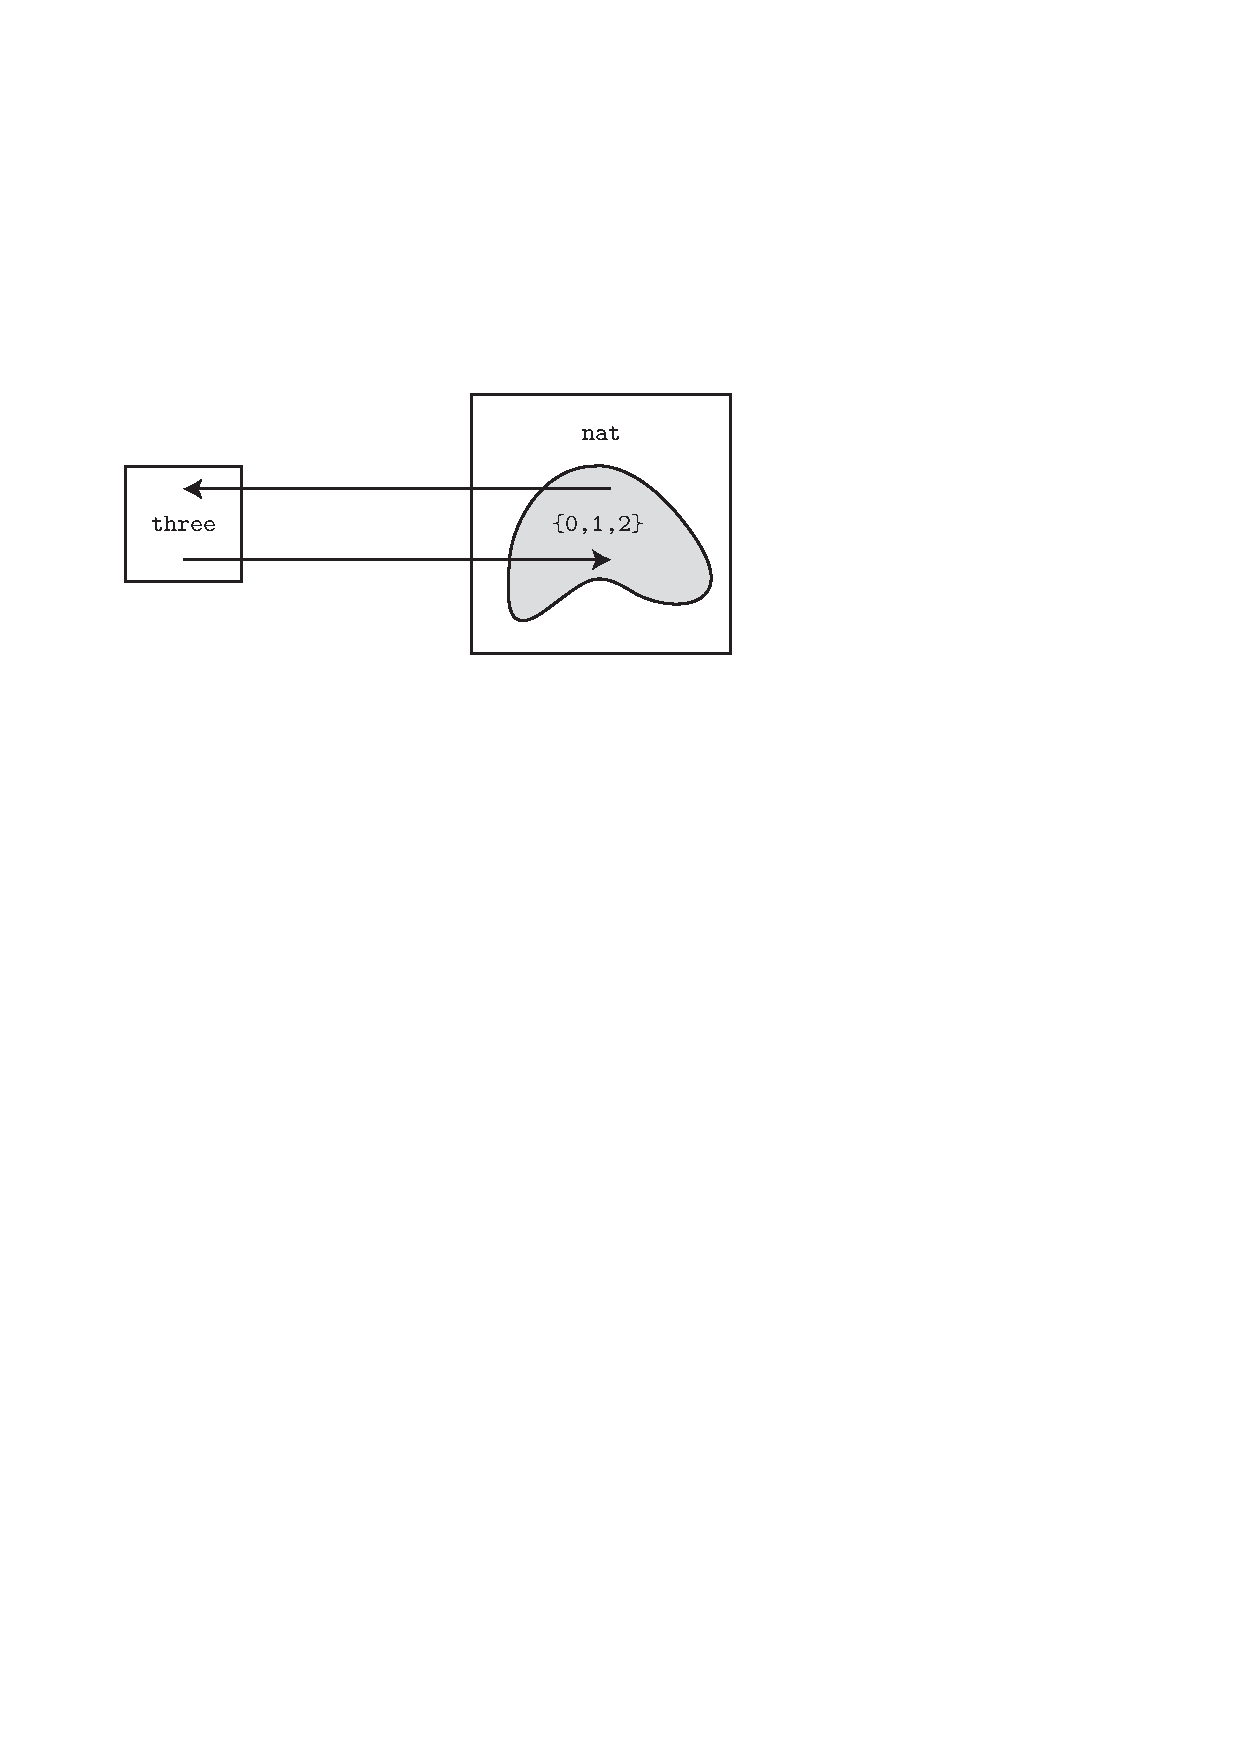
\includegraphics[scale=.8]{typedef}
\end{center}
Finally, \isacommand{typedef} asserts that \isa{Rep{\isacharunderscore}three} is
surjective on the subset \isa{three} and \isa{Abs{\isacharunderscore}three} and \isa{Rep{\isacharunderscore}three} are inverses of each other:
\begin{center}
\begin{tabular}{@ {}r@ {\qquad\qquad}l@ {}}
\isa{Rep{\isacharunderscore}three\ x\ {\isasymin}\ three} & (\isa{Rep{\isacharunderscore}three}) \\
\isa{Abs{\isacharunderscore}three\ {\isacharparenleft}Rep{\isacharunderscore}three\ x{\isacharparenright}\ {\isacharequal}\ x} & (\isa{Rep{\isacharunderscore}three{\isacharunderscore}inverse}) \\
\isa{y\ {\isasymin}\ three\ {\isasymLongrightarrow}\ Rep{\isacharunderscore}three\ {\isacharparenleft}Abs{\isacharunderscore}three\ y{\isacharparenright}\ {\isacharequal}\ y} & (\isa{Abs{\isacharunderscore}three{\isacharunderscore}inverse})
\end{tabular}
\end{center}
%
From this example it should be clear what \isacommand{typedef} does
in general given a name (here \isa{three}) and a set
(here \isa{{\isacharbraceleft}{\isadigit{0}}{\isacharcomma}\ {\isadigit{1}}{\isacharcomma}\ {\isadigit{2}}{\isacharbraceright}}).

Our next step is to define the basic functions expected on the new type.
Although this depends on the type at hand, the following strategy works well:
\begin{itemize}
\item define a small kernel of basic functions that can express all other
functions you anticipate.
\item define the kernel in terms of corresponding functions on the
representing type using \isa{Abs} and \isa{Rep} to convert between the
two levels.
\end{itemize}
In our example it suffices to give the three elements of type \isa{three}
names:%
\end{isamarkuptext}%
\isamarkuptrue%
\isacommand{constdefs}\isanewline
\ \ A{\isacharcolon}{\isacharcolon}\ three\isanewline
\ {\isachardoublequote}A\ {\isasymequiv}\ Abs{\isacharunderscore}three\ {\isadigit{0}}{\isachardoublequote}\isanewline
\ \ B{\isacharcolon}{\isacharcolon}\ three\isanewline
\ {\isachardoublequote}B\ {\isasymequiv}\ Abs{\isacharunderscore}three\ {\isadigit{1}}{\isachardoublequote}\isanewline
\ \ C\ {\isacharcolon}{\isacharcolon}\ three\isanewline
\ {\isachardoublequote}C\ {\isasymequiv}\ Abs{\isacharunderscore}three\ {\isadigit{2}}{\isachardoublequote}\isamarkupfalse%
%
\begin{isamarkuptext}%
So far, everything was easy. But it is clear that reasoning about \isa{three} will be hell if we have to go back to \isa{nat} every time. Thus our
aim must be to raise our level of abstraction by deriving enough theorems
about type \isa{three} to characterize it completely. And those theorems
should be phrased in terms of \isa{A}, \isa{B} and \isa{C}, not \isa{Abs{\isacharunderscore}three} and \isa{Rep{\isacharunderscore}three}. Because of the simplicity of the example,
we merely need to prove that \isa{A}, \isa{B} and \isa{C} are distinct
and that they exhaust the type.

In processing our \isacommand{typedef} declaration, 
Isabelle proves several helpful lemmas. The first two
express injectivity of \isa{Rep{\isacharunderscore}three} and \isa{Abs{\isacharunderscore}three}:
\begin{center}
\begin{tabular}{@ {}r@ {\qquad}l@ {}}
\isa{{\isacharparenleft}Rep{\isacharunderscore}three\ x\ {\isacharequal}\ Rep{\isacharunderscore}three\ y{\isacharparenright}\ {\isacharequal}\ {\isacharparenleft}x\ {\isacharequal}\ y{\isacharparenright}} & (\isa{Rep{\isacharunderscore}three{\isacharunderscore}inject}) \\
\begin{tabular}{@ {}l@ {}}
\isa{{\isasymlbrakk}x\ {\isasymin}\ three{\isacharsemicolon}\ y\ {\isasymin}\ three\ {\isasymrbrakk}} \\
\isa{{\isasymLongrightarrow}\ {\isacharparenleft}Abs{\isacharunderscore}three\ x\ {\isacharequal}\ Abs{\isacharunderscore}three\ y{\isacharparenright}\ {\isacharequal}\ {\isacharparenleft}x\ {\isacharequal}\ y{\isacharparenright}}
\end{tabular} & (\isa{Abs{\isacharunderscore}three{\isacharunderscore}inject}) \\
\end{tabular}
\end{center}
The following ones allow to replace some \isa{x{\isacharcolon}{\isacharcolon}three} by
\isa{Abs{\isacharunderscore}three{\isacharparenleft}y{\isacharcolon}{\isacharcolon}nat{\isacharparenright}}, and conversely \isa{y} by \isa{Rep{\isacharunderscore}three\ x}:
\begin{center}
\begin{tabular}{@ {}r@ {\qquad}l@ {}}
\isa{{\isasymlbrakk}y\ {\isasymin}\ three{\isacharsemicolon}\ {\isasymAnd}x{\isachardot}\ y\ {\isacharequal}\ Rep{\isacharunderscore}three\ x\ {\isasymLongrightarrow}\ P{\isasymrbrakk}\ {\isasymLongrightarrow}\ P} & (\isa{Rep{\isacharunderscore}three{\isacharunderscore}cases}) \\
\isa{{\isacharparenleft}{\isasymAnd}y{\isachardot}\ {\isasymlbrakk}x\ {\isacharequal}\ Abs{\isacharunderscore}three\ y{\isacharsemicolon}\ y\ {\isasymin}\ three{\isasymrbrakk}\ {\isasymLongrightarrow}\ P{\isacharparenright}\ {\isasymLongrightarrow}\ P} & (\isa{Abs{\isacharunderscore}three{\isacharunderscore}cases}) \\
\isa{{\isasymlbrakk}y\ {\isasymin}\ three{\isacharsemicolon}\ {\isasymAnd}x{\isachardot}\ P\ {\isacharparenleft}Rep{\isacharunderscore}three\ x{\isacharparenright}{\isasymrbrakk}\ {\isasymLongrightarrow}\ P\ y} & (\isa{Rep{\isacharunderscore}three{\isacharunderscore}induct}) \\
\isa{{\isacharparenleft}{\isasymAnd}y{\isachardot}\ y\ {\isasymin}\ three\ {\isasymLongrightarrow}\ P\ {\isacharparenleft}Abs{\isacharunderscore}three\ y{\isacharparenright}{\isacharparenright}\ {\isasymLongrightarrow}\ P\ x} & (\isa{Abs{\isacharunderscore}three{\isacharunderscore}induct}) \\
\end{tabular}
\end{center}
These theorems are proved for any type definition, with \isa{three}
replaced by the name of the type in question.

Distinctness of \isa{A}, \isa{B} and \isa{C} follows immediately
if we expand their definitions and rewrite with the injectivity
of \isa{Abs{\isacharunderscore}three}:%
\end{isamarkuptext}%
\isamarkuptrue%
\isacommand{lemma}\ {\isachardoublequote}A\ {\isasymnoteq}\ B\ {\isasymand}\ B\ {\isasymnoteq}\ A\ {\isasymand}\ A\ {\isasymnoteq}\ C\ {\isasymand}\ C\ {\isasymnoteq}\ A\ {\isasymand}\ B\ {\isasymnoteq}\ C\ {\isasymand}\ C\ {\isasymnoteq}\ B{\isachardoublequote}\isanewline
\isamarkupfalse%
\isacommand{by}{\isacharparenleft}simp\ add{\isacharcolon}\ Abs{\isacharunderscore}three{\isacharunderscore}inject\ A{\isacharunderscore}def\ B{\isacharunderscore}def\ C{\isacharunderscore}def\ three{\isacharunderscore}def{\isacharparenright}\isamarkupfalse%
%
\begin{isamarkuptext}%
\noindent
Of course we rely on the simplifier to solve goals like \isa{{\isadigit{0}}\ {\isasymnoteq}\ {\isadigit{1}}}.

The fact that \isa{A}, \isa{B} and \isa{C} exhaust type \isa{three} is
best phrased as a case distinction theorem: if you want to prove \isa{P\ x}
(where \isa{x} is of type \isa{three}) it suffices to prove \isa{P\ A},
\isa{P\ B} and \isa{P\ C}:%
\end{isamarkuptext}%
\isamarkuptrue%
\isacommand{lemma}\ three{\isacharunderscore}cases{\isacharcolon}\ {\isachardoublequote}{\isasymlbrakk}\ P\ A{\isacharsemicolon}\ P\ B{\isacharsemicolon}\ P\ C\ {\isasymrbrakk}\ {\isasymLongrightarrow}\ P\ x{\isachardoublequote}\isamarkupfalse%
%
\begin{isamarkuptxt}%
\noindent Again this follows easily from a pre-proved general theorem:%
\end{isamarkuptxt}%
\isamarkuptrue%
\isacommand{apply}{\isacharparenleft}induct{\isacharunderscore}tac\ x\ rule{\isacharcolon}\ Abs{\isacharunderscore}three{\isacharunderscore}induct{\isacharparenright}\isamarkupfalse%
%
\begin{isamarkuptxt}%
\begin{isabelle}%
\ {\isadigit{1}}{\isachardot}\ {\isasymAnd}y{\isachardot}\ {\isasymlbrakk}P\ A{\isacharsemicolon}\ P\ B{\isacharsemicolon}\ P\ C{\isacharsemicolon}\ y\ {\isasymin}\ three{\isasymrbrakk}\ {\isasymLongrightarrow}\ P\ {\isacharparenleft}Abs{\isacharunderscore}three\ y{\isacharparenright}%
\end{isabelle}
Simplification with \isa{three{\isacharunderscore}def} leads to the disjunction \isa{y\ {\isacharequal}\ {\isadigit{0}}\ {\isasymor}\ y\ {\isacharequal}\ {\isadigit{1}}\ {\isasymor}\ y\ {\isacharequal}\ {\isadigit{2}}} which \isa{auto} separates into three
subgoals, each of which is easily solved by simplification:%
\end{isamarkuptxt}%
\isamarkuptrue%
\isacommand{apply}{\isacharparenleft}auto\ simp\ add{\isacharcolon}\ three{\isacharunderscore}def\ A{\isacharunderscore}def\ B{\isacharunderscore}def\ C{\isacharunderscore}def{\isacharparenright}\isanewline
\isamarkupfalse%
\isacommand{done}\isamarkupfalse%
%
\begin{isamarkuptext}%
\noindent
This concludes the derivation of the characteristic theorems for
type \isa{three}.

The attentive reader has realized long ago that the
above lengthy definition can be collapsed into one line:%
\end{isamarkuptext}%
\isamarkuptrue%
\isacommand{datatype}\ better{\isacharunderscore}three\ {\isacharequal}\ A\ {\isacharbar}\ B\ {\isacharbar}\ C\isamarkupfalse%
%
\begin{isamarkuptext}%
\noindent
In fact, the \isacommand{datatype} command performs internally more or less
the same derivations as we did, which gives you some idea what life would be
like without \isacommand{datatype}.

Although \isa{three} could be defined in one line, we have chosen this
example to demonstrate \isacommand{typedef} because its simplicity makes the
key concepts particularly easy to grasp. If you would like to see a
non-trivial example that cannot be defined more directly, we recommend the
definition of \emph{finite multisets} in the Library~\cite{HOL-Library}.

Let us conclude by summarizing the above procedure for defining a new type.
Given some abstract axiomatic description $P$ of a type $ty$ in terms of a
set of functions $F$, this involves three steps:
\begin{enumerate}
\item Find an appropriate type $\tau$ and subset $A$ which has the desired
  properties $P$, and make a type definition based on this representation.
\item Define the required functions $F$ on $ty$ by lifting
analogous functions on the representation via $Abs_ty$ and $Rep_ty$.
\item Prove that $P$ holds for $ty$ by lifting $P$ from the representation.
\end{enumerate}
You can now forget about the representation and work solely in terms of the
abstract functions $F$ and properties $P$.%
\index{typedecl@\isacommand {typedef} (command)|)}%
\index{types!defining|)}%
\end{isamarkuptext}%
\isamarkuptrue%
\isamarkupfalse%
\end{isabellebody}%
%%% Local Variables:
%%% mode: latex
%%% TeX-master: "root"
%%% End:
    %%%Section "Introducing New Types"

\chapter{Advanced Simplification and Induction}

Although we have already learned a lot about simplification and
induction, there are some advanced proof techniques that we have not covered
yet and which are worth learning. The sections of this chapter are
independent of each other and can be read in any order.

%
\begin{isabellebody}%
\def\isabellecontext{simp{\isadigit{2}}}%
%
\isadelimtheory
%
\endisadelimtheory
%
\isatagtheory
%
\endisatagtheory
{\isafoldtheory}%
%
\isadelimtheory
%
\endisadelimtheory
%
\isamarkupsection{Simplification%
}
\isamarkuptrue%
%
\begin{isamarkuptext}%
\label{sec:simplification-II}\index{simplification|(}
This section describes features not covered until now.  It also
outlines the simplification process itself, which can be helpful
when the simplifier does not do what you expect of it.%
\end{isamarkuptext}%
\isamarkuptrue%
%
\isamarkupsubsection{Advanced Features%
}
\isamarkuptrue%
%
\isamarkupsubsubsection{Congruence Rules%
}
\isamarkuptrue%
%
\begin{isamarkuptext}%
\label{sec:simp-cong}
While simplifying the conclusion $Q$
of $P \Imp Q$, it is legal to use the assumption $P$.
For $\Imp$ this policy is hardwired, but 
contextual information can also be made available for other
operators. For example, \isa{xs\ {\isaliteral{3D}{\isacharequal}}\ {\isaliteral{5B}{\isacharbrackleft}}{\isaliteral{5D}{\isacharbrackright}}\ {\isaliteral{5C3C6C6F6E6772696768746172726F773E}{\isasymlongrightarrow}}\ xs\ {\isaliteral{40}{\isacharat}}\ xs\ {\isaliteral{3D}{\isacharequal}}\ xs} simplifies to \isa{True} because we may use \isa{xs\ {\isaliteral{3D}{\isacharequal}}\ {\isaliteral{5B}{\isacharbrackleft}}{\isaliteral{5D}{\isacharbrackright}}} when simplifying \isa{xs\ {\isaliteral{40}{\isacharat}}\ xs\ {\isaliteral{3D}{\isacharequal}}\ xs}. The generation of contextual information during simplification is
controlled by so-called \bfindex{congruence rules}. This is the one for
\isa{{\isaliteral{5C3C6C6F6E6772696768746172726F773E}{\isasymlongrightarrow}}}:
\begin{isabelle}%
\ \ \ \ \ {\isaliteral{5C3C6C6272616B6B3E}{\isasymlbrakk}}P\ {\isaliteral{3D}{\isacharequal}}\ P{\isaliteral{27}{\isacharprime}}{\isaliteral{3B}{\isacharsemicolon}}\ P{\isaliteral{27}{\isacharprime}}\ {\isaliteral{5C3C4C6F6E6772696768746172726F773E}{\isasymLongrightarrow}}\ Q\ {\isaliteral{3D}{\isacharequal}}\ Q{\isaliteral{27}{\isacharprime}}{\isaliteral{5C3C726272616B6B3E}{\isasymrbrakk}}\ {\isaliteral{5C3C4C6F6E6772696768746172726F773E}{\isasymLongrightarrow}}\ {\isaliteral{28}{\isacharparenleft}}P\ {\isaliteral{5C3C6C6F6E6772696768746172726F773E}{\isasymlongrightarrow}}\ Q{\isaliteral{29}{\isacharparenright}}\ {\isaliteral{3D}{\isacharequal}}\ {\isaliteral{28}{\isacharparenleft}}P{\isaliteral{27}{\isacharprime}}\ {\isaliteral{5C3C6C6F6E6772696768746172726F773E}{\isasymlongrightarrow}}\ Q{\isaliteral{27}{\isacharprime}}{\isaliteral{29}{\isacharparenright}}%
\end{isabelle}
It should be read as follows:
In order to simplify \isa{P\ {\isaliteral{5C3C6C6F6E6772696768746172726F773E}{\isasymlongrightarrow}}\ Q} to \isa{P{\isaliteral{27}{\isacharprime}}\ {\isaliteral{5C3C6C6F6E6772696768746172726F773E}{\isasymlongrightarrow}}\ Q{\isaliteral{27}{\isacharprime}}},
simplify \isa{P} to \isa{P{\isaliteral{27}{\isacharprime}}}
and assume \isa{P{\isaliteral{27}{\isacharprime}}} when simplifying \isa{Q} to \isa{Q{\isaliteral{27}{\isacharprime}}}.

Here are some more examples.  The congruence rules for bounded
quantifiers supply contextual information about the bound variable:
\begin{isabelle}%
\ \ \ \ \ {\isaliteral{5C3C6C6272616B6B3E}{\isasymlbrakk}}A\ {\isaliteral{3D}{\isacharequal}}\ B{\isaliteral{3B}{\isacharsemicolon}}\ {\isaliteral{5C3C416E643E}{\isasymAnd}}x{\isaliteral{2E}{\isachardot}}\ x\ {\isaliteral{5C3C696E3E}{\isasymin}}\ B\ {\isaliteral{5C3C4C6F6E6772696768746172726F773E}{\isasymLongrightarrow}}\ P\ x\ {\isaliteral{3D}{\isacharequal}}\ Q\ x{\isaliteral{5C3C726272616B6B3E}{\isasymrbrakk}}\isanewline
\isaindent{\ \ \ \ \ }{\isaliteral{5C3C4C6F6E6772696768746172726F773E}{\isasymLongrightarrow}}\ {\isaliteral{28}{\isacharparenleft}}{\isaliteral{5C3C666F72616C6C3E}{\isasymforall}}x{\isaliteral{5C3C696E3E}{\isasymin}}A{\isaliteral{2E}{\isachardot}}\ P\ x{\isaliteral{29}{\isacharparenright}}\ {\isaliteral{3D}{\isacharequal}}\ {\isaliteral{28}{\isacharparenleft}}{\isaliteral{5C3C666F72616C6C3E}{\isasymforall}}x{\isaliteral{5C3C696E3E}{\isasymin}}B{\isaliteral{2E}{\isachardot}}\ Q\ x{\isaliteral{29}{\isacharparenright}}%
\end{isabelle}
One congruence rule for conditional expressions supplies contextual
information for simplifying the \isa{then} and \isa{else} cases:
\begin{isabelle}%
\ \ \ \ \ {\isaliteral{5C3C6C6272616B6B3E}{\isasymlbrakk}}b\ {\isaliteral{3D}{\isacharequal}}\ c{\isaliteral{3B}{\isacharsemicolon}}\ c\ {\isaliteral{5C3C4C6F6E6772696768746172726F773E}{\isasymLongrightarrow}}\ x\ {\isaliteral{3D}{\isacharequal}}\ u{\isaliteral{3B}{\isacharsemicolon}}\ {\isaliteral{5C3C6E6F743E}{\isasymnot}}\ c\ {\isaliteral{5C3C4C6F6E6772696768746172726F773E}{\isasymLongrightarrow}}\ y\ {\isaliteral{3D}{\isacharequal}}\ v{\isaliteral{5C3C726272616B6B3E}{\isasymrbrakk}}\isanewline
\isaindent{\ \ \ \ \ }{\isaliteral{5C3C4C6F6E6772696768746172726F773E}{\isasymLongrightarrow}}\ {\isaliteral{28}{\isacharparenleft}}if\ b\ then\ x\ else\ y{\isaliteral{29}{\isacharparenright}}\ {\isaliteral{3D}{\isacharequal}}\ {\isaliteral{28}{\isacharparenleft}}if\ c\ then\ u\ else\ v{\isaliteral{29}{\isacharparenright}}%
\end{isabelle}
An alternative congruence rule for conditional expressions
actually \emph{prevents} simplification of some arguments:
\begin{isabelle}%
\ \ \ \ \ b\ {\isaliteral{3D}{\isacharequal}}\ c\ {\isaliteral{5C3C4C6F6E6772696768746172726F773E}{\isasymLongrightarrow}}\ {\isaliteral{28}{\isacharparenleft}}if\ b\ then\ x\ else\ y{\isaliteral{29}{\isacharparenright}}\ {\isaliteral{3D}{\isacharequal}}\ {\isaliteral{28}{\isacharparenleft}}if\ c\ then\ x\ else\ y{\isaliteral{29}{\isacharparenright}}%
\end{isabelle}
Only the first argument is simplified; the others remain unchanged.
This makes simplification much faster and is faithful to the evaluation
strategy in programming languages, which is why this is the default
congruence rule for \isa{if}. Analogous rules control the evaluation of
\isa{case} expressions.

You can declare your own congruence rules with the attribute \attrdx{cong},
either globally, in the usual manner,
\begin{quote}
\isacommand{declare} \textit{theorem-name} \isa{{\isaliteral{5B}{\isacharbrackleft}}cong{\isaliteral{5D}{\isacharbrackright}}}
\end{quote}
or locally in a \isa{simp} call by adding the modifier
\begin{quote}
\isa{cong{\isaliteral{3A}{\isacharcolon}}} \textit{list of theorem names}
\end{quote}
The effect is reversed by \isa{cong\ del} instead of \isa{cong}.

\begin{warn}
The congruence rule \isa{conj{\isaliteral{5F}{\isacharunderscore}}cong}
\begin{isabelle}%
\ \ \ \ \ {\isaliteral{5C3C6C6272616B6B3E}{\isasymlbrakk}}P\ {\isaliteral{3D}{\isacharequal}}\ P{\isaliteral{27}{\isacharprime}}{\isaliteral{3B}{\isacharsemicolon}}\ P{\isaliteral{27}{\isacharprime}}\ {\isaliteral{5C3C4C6F6E6772696768746172726F773E}{\isasymLongrightarrow}}\ Q\ {\isaliteral{3D}{\isacharequal}}\ Q{\isaliteral{27}{\isacharprime}}{\isaliteral{5C3C726272616B6B3E}{\isasymrbrakk}}\ {\isaliteral{5C3C4C6F6E6772696768746172726F773E}{\isasymLongrightarrow}}\ {\isaliteral{28}{\isacharparenleft}}P\ {\isaliteral{5C3C616E643E}{\isasymand}}\ Q{\isaliteral{29}{\isacharparenright}}\ {\isaliteral{3D}{\isacharequal}}\ {\isaliteral{28}{\isacharparenleft}}P{\isaliteral{27}{\isacharprime}}\ {\isaliteral{5C3C616E643E}{\isasymand}}\ Q{\isaliteral{27}{\isacharprime}}{\isaliteral{29}{\isacharparenright}}%
\end{isabelle}
\par\noindent
is occasionally useful but is not a default rule; you have to declare it explicitly.
\end{warn}%
\end{isamarkuptext}%
\isamarkuptrue%
%
\isamarkupsubsubsection{Permutative Rewrite Rules%
}
\isamarkuptrue%
%
\begin{isamarkuptext}%
\index{rewrite rules!permutative|bold}%
An equation is a \textbf{permutative rewrite rule} if the left-hand
side and right-hand side are the same up to renaming of variables.  The most
common permutative rule is commutativity: \isa{x\ {\isaliteral{2B}{\isacharplus}}\ y\ {\isaliteral{3D}{\isacharequal}}\ y\ {\isaliteral{2B}{\isacharplus}}\ x}.  Other examples
include \isa{x\ {\isaliteral{2D}{\isacharminus}}\ y\ {\isaliteral{2D}{\isacharminus}}\ z\ {\isaliteral{3D}{\isacharequal}}\ x\ {\isaliteral{2D}{\isacharminus}}\ z\ {\isaliteral{2D}{\isacharminus}}\ y} in arithmetic and \isa{insert\ x\ {\isaliteral{28}{\isacharparenleft}}insert\ y\ A{\isaliteral{29}{\isacharparenright}}\ {\isaliteral{3D}{\isacharequal}}\ insert\ y\ {\isaliteral{28}{\isacharparenleft}}insert\ x\ A{\isaliteral{29}{\isacharparenright}}} for sets. Such rules are problematic because
once they apply, they can be used forever. The simplifier is aware of this
danger and treats permutative rules by means of a special strategy, called
\bfindex{ordered rewriting}: a permutative rewrite
rule is only applied if the term becomes smaller with respect to a fixed
lexicographic ordering on terms. For example, commutativity rewrites
\isa{b\ {\isaliteral{2B}{\isacharplus}}\ a} to \isa{a\ {\isaliteral{2B}{\isacharplus}}\ b}, but then stops because \isa{a\ {\isaliteral{2B}{\isacharplus}}\ b} is strictly
smaller than \isa{b\ {\isaliteral{2B}{\isacharplus}}\ a}.  Permutative rewrite rules can be turned into
simplification rules in the usual manner via the \isa{simp} attribute; the
simplifier recognizes their special status automatically.

Permutative rewrite rules are most effective in the case of
associative-commutative functions.  (Associativity by itself is not
permutative.)  When dealing with an AC-function~$f$, keep the
following points in mind:
\begin{itemize}\index{associative-commutative function}
  
\item The associative law must always be oriented from left to right,
  namely $f(f(x,y),z) = f(x,f(y,z))$.  The opposite orientation, if
  used with commutativity, can lead to nontermination.

\item To complete your set of rewrite rules, you must add not just
  associativity~(A) and commutativity~(C) but also a derived rule, {\bf
    left-com\-mut\-ativ\-ity} (LC): $f(x,f(y,z)) = f(y,f(x,z))$.
\end{itemize}
Ordered rewriting with the combination of A, C, and LC sorts a term
lexicographically:
\[\def\maps#1{~\stackrel{#1}{\leadsto}~}
 f(f(b,c),a) \maps{A} f(b,f(c,a)) \maps{C} f(b,f(a,c)) \maps{LC} f(a,f(b,c)) \]

Note that ordered rewriting for \isa{{\isaliteral{2B}{\isacharplus}}} and \isa{{\isaliteral{2A}{\isacharasterisk}}} on numbers is rarely
necessary because the built-in arithmetic prover often succeeds without
such tricks.%
\end{isamarkuptext}%
\isamarkuptrue%
%
\isamarkupsubsection{How the Simplifier Works%
}
\isamarkuptrue%
%
\begin{isamarkuptext}%
\label{sec:SimpHow}
Roughly speaking, the simplifier proceeds bottom-up: subterms are simplified
first.  A conditional equation is only applied if its condition can be
proved, again by simplification.  Below we explain some special features of
the rewriting process.%
\end{isamarkuptext}%
\isamarkuptrue%
%
\isamarkupsubsubsection{Higher-Order Patterns%
}
\isamarkuptrue%
%
\begin{isamarkuptext}%
\index{simplification rule|(}
So far we have pretended the simplifier can deal with arbitrary
rewrite rules. This is not quite true.  For reasons of feasibility,
the simplifier expects the
left-hand side of each rule to be a so-called \emph{higher-order
pattern}~\cite{nipkow-patterns}\indexbold{patterns!higher-order}. 
This restricts where
unknowns may occur.  Higher-order patterns are terms in $\beta$-normal
form.  (This means there are no subterms of the form $(\lambda x. M)(N)$.)  
Each occurrence of an unknown is of the form
$\Var{f}~x@1~\dots~x@n$, where the $x@i$ are distinct bound
variables. Thus all ordinary rewrite rules, where all unknowns are
of base type, for example \isa{{\isaliteral{3F}{\isacharquery}}a\ {\isaliteral{2B}{\isacharplus}}\ {\isaliteral{3F}{\isacharquery}}b\ {\isaliteral{2B}{\isacharplus}}\ {\isaliteral{3F}{\isacharquery}}c\ {\isaliteral{3D}{\isacharequal}}\ {\isaliteral{3F}{\isacharquery}}a\ {\isaliteral{2B}{\isacharplus}}\ {\isaliteral{28}{\isacharparenleft}}{\isaliteral{3F}{\isacharquery}}b\ {\isaliteral{2B}{\isacharplus}}\ {\isaliteral{3F}{\isacharquery}}c{\isaliteral{29}{\isacharparenright}}}, are acceptable: if an unknown is
of base type, it cannot have any arguments. Additionally, the rule
\isa{{\isaliteral{28}{\isacharparenleft}}{\isaliteral{5C3C666F72616C6C3E}{\isasymforall}}x{\isaliteral{2E}{\isachardot}}\ {\isaliteral{3F}{\isacharquery}}P\ x\ {\isaliteral{5C3C616E643E}{\isasymand}}\ {\isaliteral{3F}{\isacharquery}}Q\ x{\isaliteral{29}{\isacharparenright}}\ {\isaliteral{3D}{\isacharequal}}\ {\isaliteral{28}{\isacharparenleft}}{\isaliteral{28}{\isacharparenleft}}{\isaliteral{5C3C666F72616C6C3E}{\isasymforall}}x{\isaliteral{2E}{\isachardot}}\ {\isaliteral{3F}{\isacharquery}}P\ x{\isaliteral{29}{\isacharparenright}}\ {\isaliteral{5C3C616E643E}{\isasymand}}\ {\isaliteral{28}{\isacharparenleft}}{\isaliteral{5C3C666F72616C6C3E}{\isasymforall}}x{\isaliteral{2E}{\isachardot}}\ {\isaliteral{3F}{\isacharquery}}Q\ x{\isaliteral{29}{\isacharparenright}}{\isaliteral{29}{\isacharparenright}}} is also acceptable, in
both directions: all arguments of the unknowns \isa{{\isaliteral{3F}{\isacharquery}}P} and
\isa{{\isaliteral{3F}{\isacharquery}}Q} are distinct bound variables.

If the left-hand side is not a higher-order pattern, all is not lost.
The simplifier will still try to apply the rule provided it
matches directly: without much $\lambda$-calculus hocus
pocus.  For example, \isa{{\isaliteral{28}{\isacharparenleft}}{\isaliteral{3F}{\isacharquery}}f\ {\isaliteral{3F}{\isacharquery}}x\ {\isaliteral{5C3C696E3E}{\isasymin}}\ range\ {\isaliteral{3F}{\isacharquery}}f{\isaliteral{29}{\isacharparenright}}\ {\isaliteral{3D}{\isacharequal}}\ True} rewrites
\isa{g\ a\ {\isaliteral{5C3C696E3E}{\isasymin}}\ range\ g} to \isa{True}, but will fail to match
\isa{g{\isaliteral{28}{\isacharparenleft}}h\ b{\isaliteral{29}{\isacharparenright}}\ {\isaliteral{5C3C696E3E}{\isasymin}}\ range{\isaliteral{28}{\isacharparenleft}}{\isaliteral{5C3C6C616D6264613E}{\isasymlambda}}x{\isaliteral{2E}{\isachardot}}\ g{\isaliteral{28}{\isacharparenleft}}h\ x{\isaliteral{29}{\isacharparenright}}{\isaliteral{29}{\isacharparenright}}}.  However, you can
eliminate the offending subterms --- those that are not patterns ---
by adding new variables and conditions.
In our example, we eliminate \isa{{\isaliteral{3F}{\isacharquery}}f\ {\isaliteral{3F}{\isacharquery}}x} and obtain
 \isa{{\isaliteral{3F}{\isacharquery}}y\ {\isaliteral{3D}{\isacharequal}}\ {\isaliteral{3F}{\isacharquery}}f\ {\isaliteral{3F}{\isacharquery}}x\ {\isaliteral{5C3C4C6F6E6772696768746172726F773E}{\isasymLongrightarrow}}\ {\isaliteral{28}{\isacharparenleft}}{\isaliteral{3F}{\isacharquery}}y\ {\isaliteral{5C3C696E3E}{\isasymin}}\ range\ {\isaliteral{3F}{\isacharquery}}f{\isaliteral{29}{\isacharparenright}}\ {\isaliteral{3D}{\isacharequal}}\ True}, which is fine
as a conditional rewrite rule since conditions can be arbitrary
terms.  However, this trick is not a panacea because the newly
introduced conditions may be hard to solve.
  
There is no restriction on the form of the right-hand
sides.  They may not contain extraneous term or type variables, though.%
\end{isamarkuptext}%
\isamarkuptrue%
%
\isamarkupsubsubsection{The Preprocessor%
}
\isamarkuptrue%
%
\begin{isamarkuptext}%
\label{sec:simp-preprocessor}
When a theorem is declared a simplification rule, it need not be a
conditional equation already.  The simplifier will turn it into a set of
conditional equations automatically.  For example, \isa{f\ x\ {\isaliteral{3D}{\isacharequal}}\ g\ x\ {\isaliteral{5C3C616E643E}{\isasymand}}\ h\ x\ {\isaliteral{3D}{\isacharequal}}\ k\ x} becomes the two separate
simplification rules \isa{f\ x\ {\isaliteral{3D}{\isacharequal}}\ g\ x} and \isa{h\ x\ {\isaliteral{3D}{\isacharequal}}\ k\ x}. In
general, the input theorem is converted as follows:
\begin{eqnarray}
\neg P &\mapsto& P = \hbox{\isa{False}} \nonumber\\
P \longrightarrow Q &\mapsto& P \Longrightarrow Q \nonumber\\
P \land Q &\mapsto& P,\ Q \nonumber\\
\forall x.~P~x &\mapsto& P~\Var{x}\nonumber\\
\forall x \in A.\ P~x &\mapsto& \Var{x} \in A \Longrightarrow P~\Var{x} \nonumber\\
\isa{if}\ P\ \isa{then}\ Q\ \isa{else}\ R &\mapsto&
 P \Longrightarrow Q,\ \neg P \Longrightarrow R \nonumber
\end{eqnarray}
Once this conversion process is finished, all remaining non-equations
$P$ are turned into trivial equations $P =\isa{True}$.
For example, the formula 
\begin{center}\isa{{\isaliteral{28}{\isacharparenleft}}p\ {\isaliteral{5C3C6C6F6E6772696768746172726F773E}{\isasymlongrightarrow}}\ t\ {\isaliteral{3D}{\isacharequal}}\ u\ {\isaliteral{5C3C616E643E}{\isasymand}}\ {\isaliteral{5C3C6E6F743E}{\isasymnot}}\ r{\isaliteral{29}{\isacharparenright}}\ {\isaliteral{5C3C616E643E}{\isasymand}}\ s}\end{center}
is converted into the three rules
\begin{center}
\isa{p\ {\isaliteral{5C3C4C6F6E6772696768746172726F773E}{\isasymLongrightarrow}}\ t\ {\isaliteral{3D}{\isacharequal}}\ u},\quad  \isa{p\ {\isaliteral{5C3C4C6F6E6772696768746172726F773E}{\isasymLongrightarrow}}\ r\ {\isaliteral{3D}{\isacharequal}}\ False},\quad  \isa{s\ {\isaliteral{3D}{\isacharequal}}\ True}.
\end{center}
\index{simplification rule|)}
\index{simplification|)}%
\end{isamarkuptext}%
\isamarkuptrue%
%
\isadelimtheory
%
\endisadelimtheory
%
\isatagtheory
%
\endisatagtheory
{\isafoldtheory}%
%
\isadelimtheory
%
\endisadelimtheory
\end{isabellebody}%
%%% Local Variables:
%%% mode: latex
%%% TeX-master: "root"
%%% End:


\section{Advanced Induction Techniques}
\label{sec:advanced-ind}
\index{induction|(}
%
\begin{isabellebody}%
\def\isabellecontext{AdvancedInd}%
%
\begin{isamarkuptext}%
\noindent
Now that we have learned about rules and logic, we take another look at the
finer points of induction. The two questions we answer are: what to do if the
proposition to be proved is not directly amenable to induction
(\S\ref{sec:ind-var-in-prems}), and how to utilize (\S\ref{sec:complete-ind})
and even derive (\S\ref{sec:derive-ind}) new induction schemas. We conclude
with an extended example of induction (\S\ref{sec:CTL-revisited}).%
\end{isamarkuptext}%
%
\isamarkupsubsection{Massaging the proposition}
%
\begin{isamarkuptext}%
\label{sec:ind-var-in-prems}
So far we have assumed that the theorem we want to prove is already in a form
that is amenable to induction, but this is not always the case:%
\end{isamarkuptext}%
\isacommand{lemma}\ {\isachardoublequote}xs\ {\isasymnoteq}\ {\isacharbrackleft}{\isacharbrackright}\ {\isasymLongrightarrow}\ hd{\isacharparenleft}rev\ xs{\isacharparenright}\ {\isacharequal}\ last\ xs{\isachardoublequote}\isanewline
\isacommand{apply}{\isacharparenleft}induct{\isacharunderscore}tac\ xs{\isacharparenright}%
\begin{isamarkuptxt}%
\noindent
(where \isa{hd} and \isa{last} return the first and last element of a
non-empty list)
produces the warning
\begin{quote}\tt
Induction variable occurs also among premises!
\end{quote}
and leads to the base case
\begin{isabelle}%
\ {\isadigit{1}}{\isachardot}\ xs\ {\isasymnoteq}\ {\isacharbrackleft}{\isacharbrackright}\ {\isasymLongrightarrow}\ hd\ {\isacharparenleft}rev\ {\isacharbrackleft}{\isacharbrackright}{\isacharparenright}\ {\isacharequal}\ last\ {\isacharbrackleft}{\isacharbrackright}%
\end{isabelle}
which, after simplification, becomes
\begin{isabelle}
\ 1.\ xs\ {\isasymnoteq}\ []\ {\isasymLongrightarrow}\ hd\ []\ =\ last\ []
\end{isabelle}
We cannot prove this equality because we do not know what \isa{hd} and
\isa{last} return when applied to \isa{{\isacharbrackleft}{\isacharbrackright}}.

The point is that we have violated the above warning. Because the induction
formula is only the conclusion, the occurrence of \isa{xs} in the premises is
not modified by induction. Thus the case that should have been trivial
becomes unprovable. Fortunately, the solution is easy:\footnote{A very similar
heuristic applies to rule inductions; see \S\ref{sec:rtc}.}
\begin{quote}
\emph{Pull all occurrences of the induction variable into the conclusion
using \isa{{\isasymlongrightarrow}}.}
\end{quote}
This means we should prove%
\end{isamarkuptxt}%
\isacommand{lemma}\ hd{\isacharunderscore}rev{\isacharcolon}\ {\isachardoublequote}xs\ {\isasymnoteq}\ {\isacharbrackleft}{\isacharbrackright}\ {\isasymlongrightarrow}\ hd{\isacharparenleft}rev\ xs{\isacharparenright}\ {\isacharequal}\ last\ xs{\isachardoublequote}%
\begin{isamarkuptext}%
\noindent
This time, induction leaves us with the following base case
\begin{isabelle}
\ 1.\ []\ {\isasymnoteq}\ []\ {\isasymlongrightarrow}\ hd\ (rev\ [])\ =\ last\ []
\end{isabelle}
which is trivial, and \isa{auto} finishes the whole proof.

If \isa{hd{\isacharunderscore}rev} is meant to be a simplification rule, you are
done. But if you really need the \isa{{\isasymLongrightarrow}}-version of
\isa{hd{\isacharunderscore}rev}, for example because you want to apply it as an
introduction rule, you need to derive it separately, by combining it with
modus ponens:%
\end{isamarkuptext}%
\isacommand{lemmas}\ hd{\isacharunderscore}revI\ {\isacharequal}\ hd{\isacharunderscore}rev{\isacharbrackleft}THEN\ mp{\isacharbrackright}%
\begin{isamarkuptext}%
\noindent
which yields the lemma we originally set out to prove.

In case there are multiple premises $A@1$, \dots, $A@n$ containing the
induction variable, you should turn the conclusion $C$ into
\[ A@1 \longrightarrow \cdots A@n \longrightarrow C \]
(see the remark?? in \S\ref{??}).
Additionally, you may also have to universally quantify some other variables,
which can yield a fairly complex conclusion.
Here is a simple example (which is proved by \isa{blast}):%
\end{isamarkuptext}%
\isacommand{lemma}\ simple{\isacharcolon}\ {\isachardoublequote}{\isasymforall}y{\isachardot}\ A\ y\ {\isasymlongrightarrow}\ B\ y\ {\isasymlongrightarrow}\ B\ y\ {\isasymand}\ A\ y{\isachardoublequote}%
\begin{isamarkuptext}%
\noindent
You can get the desired lemma by explicit
application of modus ponens and \isa{spec}:%
\end{isamarkuptext}%
\isacommand{lemmas}\ myrule\ {\isacharequal}\ simple{\isacharbrackleft}THEN\ spec{\isacharcomma}\ THEN\ mp{\isacharcomma}\ THEN\ mp{\isacharbrackright}%
\begin{isamarkuptext}%
\noindent
or the wholesale stripping of \isa{{\isasymforall}} and
\isa{{\isasymlongrightarrow}} in the conclusion via \isa{rule{\isacharunderscore}format}%
\end{isamarkuptext}%
\isacommand{lemmas}\ myrule\ {\isacharequal}\ simple{\isacharbrackleft}rule{\isacharunderscore}format{\isacharbrackright}%
\begin{isamarkuptext}%
\noindent
yielding \isa{{\isasymlbrakk}A\ y{\isacharsemicolon}\ B\ y{\isasymrbrakk}\ {\isasymLongrightarrow}\ B\ y\ {\isasymand}\ A\ y}.
You can go one step further and include these derivations already in the
statement of your original lemma, thus avoiding the intermediate step:%
\end{isamarkuptext}%
\isacommand{lemma}\ myrule{\isacharbrackleft}rule{\isacharunderscore}format{\isacharbrackright}{\isacharcolon}\ \ {\isachardoublequote}{\isasymforall}y{\isachardot}\ A\ y\ {\isasymlongrightarrow}\ B\ y\ {\isasymlongrightarrow}\ B\ y\ {\isasymand}\ A\ y{\isachardoublequote}%
\begin{isamarkuptext}%
\bigskip

A second reason why your proposition may not be amenable to induction is that
you want to induct on a whole term, rather than an individual variable. In
general, when inducting on some term $t$ you must rephrase the conclusion $C$
as
\[ \forall y@1 \dots y@n.~ x = t \longrightarrow C \]
where $y@1 \dots y@n$ are the free variables in $t$ and $x$ is new, and
perform induction on $x$ afterwards. An example appears in
\S\ref{sec:complete-ind} below.

The very same problem may occur in connection with rule induction. Remember
that it requires a premise of the form $(x@1,\dots,x@k) \in R$, where $R$ is
some inductively defined set and the $x@i$ are variables.  If instead we have
a premise $t \in R$, where $t$ is not just an $n$-tuple of variables, we
replace it with $(x@1,\dots,x@k) \in R$, and rephrase the conclusion $C$ as
\[ \forall y@1 \dots y@n.~ (x@1,\dots,x@k) = t \longrightarrow C \]
For an example see \S\ref{sec:CTL-revisited} below.

Of course, all premises that share free variables with $t$ need to be pulled into
the conclusion as well, under the \isa{{\isasymforall}}, again using \isa{{\isasymlongrightarrow}} as shown above.%
\end{isamarkuptext}%
%
\isamarkupsubsection{Beyond structural and recursion induction}
%
\begin{isamarkuptext}%
\label{sec:complete-ind}
So far, inductive proofs where by structural induction for
primitive recursive functions and recursion induction for total recursive
functions. But sometimes structural induction is awkward and there is no
recursive function in sight either that could furnish a more appropriate
induction schema. In such cases some existing standard induction schema can
be helpful. We show how to apply such induction schemas by an example.

Structural induction on \isa{nat} is
usually known as ``mathematical induction''. There is also ``complete
induction'', where you must prove $P(n)$ under the assumption that $P(m)$
holds for all $m<n$. In Isabelle, this is the theorem \isa{nat{\isacharunderscore}less{\isacharunderscore}induct}:
\begin{isabelle}%
\ \ \ \ \ {\isacharparenleft}{\isasymAnd}n{\isachardot}\ {\isasymforall}m{\isachardot}\ m\ {\isacharless}\ n\ {\isasymlongrightarrow}\ P\ m\ {\isasymLongrightarrow}\ P\ n{\isacharparenright}\ {\isasymLongrightarrow}\ P\ n%
\end{isabelle}
Here is an example of its application.%
\end{isamarkuptext}%
\isacommand{consts}\ f\ {\isacharcolon}{\isacharcolon}\ {\isachardoublequote}nat\ {\isasymRightarrow}\ nat{\isachardoublequote}\isanewline
\isacommand{axioms}\ f{\isacharunderscore}ax{\isacharcolon}\ {\isachardoublequote}f{\isacharparenleft}f{\isacharparenleft}n{\isacharparenright}{\isacharparenright}\ {\isacharless}\ f{\isacharparenleft}Suc{\isacharparenleft}n{\isacharparenright}{\isacharparenright}{\isachardoublequote}%
\begin{isamarkuptext}%
\noindent
From the above axiom\footnote{In general, the use of axioms is strongly
discouraged, because of the danger of inconsistencies. The above axiom does
not introduce an inconsistency because, for example, the identity function
satisfies it.}
for \isa{f} it follows that \isa{n\ {\isasymle}\ f\ n}, which can
be proved by induction on \isa{f\ n}. Following the recipe outlined
above, we have to phrase the proposition as follows to allow induction:%
\end{isamarkuptext}%
\isacommand{lemma}\ f{\isacharunderscore}incr{\isacharunderscore}lem{\isacharcolon}\ {\isachardoublequote}{\isasymforall}i{\isachardot}\ k\ {\isacharequal}\ f\ i\ {\isasymlongrightarrow}\ i\ {\isasymle}\ f\ i{\isachardoublequote}%
\begin{isamarkuptxt}%
\noindent
To perform induction on \isa{k} using \isa{nat{\isacharunderscore}less{\isacharunderscore}induct}, we use
the same general induction method as for recursion induction (see
\S\ref{sec:recdef-induction}):%
\end{isamarkuptxt}%
\isacommand{apply}{\isacharparenleft}induct{\isacharunderscore}tac\ k\ rule{\isacharcolon}\ nat{\isacharunderscore}less{\isacharunderscore}induct{\isacharparenright}%
\begin{isamarkuptxt}%
\noindent
which leaves us with the following proof state:
\begin{isabelle}%
\ {\isadigit{1}}{\isachardot}\ {\isasymAnd}n{\isachardot}\ {\isasymforall}m{\isachardot}\ m\ {\isacharless}\ n\ {\isasymlongrightarrow}\ {\isacharparenleft}{\isasymforall}i{\isachardot}\ m\ {\isacharequal}\ f\ i\ {\isasymlongrightarrow}\ i\ {\isasymle}\ f\ i{\isacharparenright}\ {\isasymLongrightarrow}\isanewline
\ \ \ \ \ \ \ \ {\isasymforall}i{\isachardot}\ n\ {\isacharequal}\ f\ i\ {\isasymlongrightarrow}\ i\ {\isasymle}\ f\ i%
\end{isabelle}
After stripping the \isa{{\isasymforall}i}, the proof continues with a case
distinction on \isa{i}. The case \isa{i\ {\isacharequal}\ {\isadigit{0}}} is trivial and we focus on
the other case:%
\end{isamarkuptxt}%
\isacommand{apply}{\isacharparenleft}rule\ allI{\isacharparenright}\isanewline
\isacommand{apply}{\isacharparenleft}case{\isacharunderscore}tac\ i{\isacharparenright}\isanewline
\ \isacommand{apply}{\isacharparenleft}simp{\isacharparenright}%
\begin{isamarkuptxt}%
\begin{isabelle}%
\ {\isadigit{1}}{\isachardot}\ {\isasymAnd}n\ i\ nat{\isachardot}\isanewline
\ \ \ \ \ \ \ {\isasymlbrakk}{\isasymforall}m{\isachardot}\ m\ {\isacharless}\ n\ {\isasymlongrightarrow}\ {\isacharparenleft}{\isasymforall}i{\isachardot}\ m\ {\isacharequal}\ f\ i\ {\isasymlongrightarrow}\ i\ {\isasymle}\ f\ i{\isacharparenright}{\isacharsemicolon}\ i\ {\isacharequal}\ Suc\ nat{\isasymrbrakk}\isanewline
\ \ \ \ \ \ \ {\isasymLongrightarrow}\ n\ {\isacharequal}\ f\ i\ {\isasymlongrightarrow}\ i\ {\isasymle}\ f\ i%
\end{isabelle}%
\end{isamarkuptxt}%
\isacommand{by}{\isacharparenleft}blast\ intro{\isacharbang}{\isacharcolon}\ f{\isacharunderscore}ax\ Suc{\isacharunderscore}leI\ intro{\isacharcolon}\ le{\isacharunderscore}less{\isacharunderscore}trans{\isacharparenright}%
\begin{isamarkuptext}%
\noindent
It is not surprising if you find the last step puzzling.
The proof goes like this (writing \isa{j} instead of \isa{nat}).
Since \isa{i\ {\isacharequal}\ Suc\ j} it suffices to show
\isa{j\ {\isacharless}\ f\ {\isacharparenleft}Suc\ j{\isacharparenright}} (by \isa{Suc{\isacharunderscore}leI}: \isa{m\ {\isacharless}\ n\ {\isasymLongrightarrow}\ Suc\ m\ {\isasymle}\ n}). This is
proved as follows. From \isa{f{\isacharunderscore}ax} we have \isa{f\ {\isacharparenleft}f\ j{\isacharparenright}\ {\isacharless}\ f\ {\isacharparenleft}Suc\ j{\isacharparenright}}
(1) which implies \isa{f\ j\ {\isasymle}\ f\ {\isacharparenleft}f\ j{\isacharparenright}} (by the induction hypothesis).
Using (1) once more we obtain \isa{f\ j\ {\isacharless}\ f\ {\isacharparenleft}Suc\ j{\isacharparenright}} (2) by transitivity
(\isa{le{\isacharunderscore}less{\isacharunderscore}trans}: \isa{{\isasymlbrakk}i\ {\isasymle}\ j{\isacharsemicolon}\ j\ {\isacharless}\ k{\isasymrbrakk}\ {\isasymLongrightarrow}\ i\ {\isacharless}\ k}).
Using the induction hypothesis once more we obtain \isa{j\ {\isasymle}\ f\ j}
which, together with (2) yields \isa{j\ {\isacharless}\ f\ {\isacharparenleft}Suc\ j{\isacharparenright}} (again by
\isa{le{\isacharunderscore}less{\isacharunderscore}trans}).

This last step shows both the power and the danger of automatic proofs: they
will usually not tell you how the proof goes, because it can be very hard to
translate the internal proof into a human-readable format. Therefore
\S\ref{sec:part2?} introduces a language for writing readable yet concise
proofs.

We can now derive the desired \isa{i\ {\isasymle}\ f\ i} from \isa{f{\isacharunderscore}incr}:%
\end{isamarkuptext}%
\isacommand{lemmas}\ f{\isacharunderscore}incr\ {\isacharequal}\ f{\isacharunderscore}incr{\isacharunderscore}lem{\isacharbrackleft}rule{\isacharunderscore}format{\isacharcomma}\ OF\ refl{\isacharbrackright}%
\begin{isamarkuptext}%
\noindent
The final \isa{refl} gets rid of the premise \isa{{\isacharquery}k\ {\isacharequal}\ f\ {\isacharquery}i}. Again,
we could have included this derivation in the original statement of the lemma:%
\end{isamarkuptext}%
\isacommand{lemma}\ f{\isacharunderscore}incr{\isacharbrackleft}rule{\isacharunderscore}format{\isacharcomma}\ OF\ refl{\isacharbrackright}{\isacharcolon}\ {\isachardoublequote}{\isasymforall}i{\isachardot}\ k\ {\isacharequal}\ f\ i\ {\isasymlongrightarrow}\ i\ {\isasymle}\ f\ i{\isachardoublequote}%
\begin{isamarkuptext}%
\begin{exercise}
From the above axiom and lemma for \isa{f} show that \isa{f} is the
identity.
\end{exercise}

In general, \isa{induct{\isacharunderscore}tac} can be applied with any rule $r$
whose conclusion is of the form ${?}P~?x@1 \dots ?x@n$, in which case the
format is
\begin{quote}
\isacommand{apply}\isa{{\isacharparenleft}induct{\isacharunderscore}tac} $y@1 \dots y@n$ \isa{rule{\isacharcolon}} $r$\isa{{\isacharparenright}}
\end{quote}\index{*induct_tac}%
where $y@1, \dots, y@n$ are variables in the first subgoal.
A further example of a useful induction rule is \isa{length{\isacharunderscore}induct},
induction on the length of a list:\indexbold{*length_induct}
\begin{isabelle}%
\ \ \ \ \ {\isacharparenleft}{\isasymAnd}xs{\isachardot}\ {\isasymforall}ys{\isachardot}\ length\ ys\ {\isacharless}\ length\ xs\ {\isasymlongrightarrow}\ P\ ys\ {\isasymLongrightarrow}\ P\ xs{\isacharparenright}\ {\isasymLongrightarrow}\ P\ xs%
\end{isabelle}

In fact, \isa{induct{\isacharunderscore}tac} even allows the conclusion of
$r$ to be an (iterated) conjunction of formulae of the above form, in
which case the application is
\begin{quote}
\isacommand{apply}\isa{{\isacharparenleft}induct{\isacharunderscore}tac} $y@1 \dots y@n$ \isa{and} \dots\ \isa{and} $z@1 \dots z@m$ \isa{rule{\isacharcolon}} $r$\isa{{\isacharparenright}}
\end{quote}%
\end{isamarkuptext}%
%
\isamarkupsubsection{Derivation of new induction schemas}
%
\begin{isamarkuptext}%
\label{sec:derive-ind}
Induction schemas are ordinary theorems and you can derive new ones
whenever you wish.  This section shows you how to, using the example
of \isa{nat{\isacharunderscore}less{\isacharunderscore}induct}. Assume we only have structural induction
available for \isa{nat} and want to derive complete induction. This
requires us to generalize the statement first:%
\end{isamarkuptext}%
\isacommand{lemma}\ induct{\isacharunderscore}lem{\isacharcolon}\ {\isachardoublequote}{\isacharparenleft}{\isasymAnd}n{\isacharcolon}{\isacharcolon}nat{\isachardot}\ {\isasymforall}m{\isacharless}n{\isachardot}\ P\ m\ {\isasymLongrightarrow}\ P\ n{\isacharparenright}\ {\isasymLongrightarrow}\ {\isasymforall}m{\isacharless}n{\isachardot}\ P\ m{\isachardoublequote}\isanewline
\isacommand{apply}{\isacharparenleft}induct{\isacharunderscore}tac\ n{\isacharparenright}%
\begin{isamarkuptxt}%
\noindent
The base case is trivially true. For the induction step (\isa{m\ {\isacharless}\ Suc\ n}) we distinguish two cases: case \isa{m\ {\isacharless}\ n} is true by induction
hypothesis and case \isa{m\ {\isacharequal}\ n} follows from the assumption, again using
the induction hypothesis:%
\end{isamarkuptxt}%
\isacommand{apply}{\isacharparenleft}blast{\isacharparenright}\isanewline
\isacommand{by}{\isacharparenleft}blast\ elim{\isacharcolon}less{\isacharunderscore}SucE{\isacharparenright}%
\begin{isamarkuptext}%
\noindent
The elimination rule \isa{less{\isacharunderscore}SucE} expresses the case distinction:
\begin{isabelle}%
\ \ \ \ \ {\isasymlbrakk}m\ {\isacharless}\ Suc\ n{\isacharsemicolon}\ m\ {\isacharless}\ n\ {\isasymLongrightarrow}\ P{\isacharsemicolon}\ m\ {\isacharequal}\ n\ {\isasymLongrightarrow}\ P{\isasymrbrakk}\ {\isasymLongrightarrow}\ P%
\end{isabelle}

Now it is straightforward to derive the original version of
\isa{nat{\isacharunderscore}less{\isacharunderscore}induct} by manipulting the conclusion of the above lemma:
instantiate \isa{n} by \isa{Suc\ n} and \isa{m} by \isa{n} and
remove the trivial condition \isa{n\ {\isacharless}\ Suc\ n}. Fortunately, this
happens automatically when we add the lemma as a new premise to the
desired goal:%
\end{isamarkuptext}%
\isacommand{theorem}\ nat{\isacharunderscore}less{\isacharunderscore}induct{\isacharcolon}\ {\isachardoublequote}{\isacharparenleft}{\isasymAnd}n{\isacharcolon}{\isacharcolon}nat{\isachardot}\ {\isasymforall}m{\isacharless}n{\isachardot}\ P\ m\ {\isasymLongrightarrow}\ P\ n{\isacharparenright}\ {\isasymLongrightarrow}\ P\ n{\isachardoublequote}\isanewline
\isacommand{by}{\isacharparenleft}insert\ induct{\isacharunderscore}lem{\isacharcomma}\ blast{\isacharparenright}%
\begin{isamarkuptext}%
Finally we should remind the reader that HOL already provides the mother of
all inductions, well-founded induction (see \S\ref{sec:Well-founded}).  For
example theorem \isa{nat{\isacharunderscore}less{\isacharunderscore}induct} can be viewed (and derived) as
a special case of \isa{wf{\isacharunderscore}induct} where \isa{r} is \isa{{\isacharless}} on
\isa{nat}. The details can be found in the HOL library.%
\end{isamarkuptext}%
\end{isabellebody}%
%%% Local Variables:
%%% mode: latex
%%% TeX-master: "root"
%%% End:

%
\begin{isabellebody}%
\def\isabellecontext{CTLind}%
%
\isamarkupsubsection{CTL Revisited%
}
%
\begin{isamarkuptext}%
\label{sec:CTL-revisited}
\index{CTL|(}%
The purpose of this section is twofold: to demonstrate
some of the induction principles and heuristics discussed above and to
show how inductive definitions can simplify proofs.
In \S\ref{sec:CTL} we gave a fairly involved proof of the correctness of a
model checker for CTL\@. In particular the proof of the
\isa{infinity{\isacharunderscore}lemma} on the way to \isa{AF{\isacharunderscore}lemma{\isadigit{2}}} is not as
simple as one might expect, due to the \isa{SOME} operator
involved. Below we give a simpler proof of \isa{AF{\isacharunderscore}lemma{\isadigit{2}}}
based on an auxiliary inductive definition.

Let us call a (finite or infinite) path \emph{\isa{A}-avoiding} if it does
not touch any node in the set \isa{A}. Then \isa{AF{\isacharunderscore}lemma{\isadigit{2}}} says
that if no infinite path from some state \isa{s} is \isa{A}-avoiding,
then \isa{s\ {\isasymin}\ lfp\ {\isacharparenleft}af\ A{\isacharparenright}}. We prove this by inductively defining the set
\isa{Avoid\ s\ A} of states reachable from \isa{s} by a finite \isa{A}-avoiding path:
% Second proof of opposite direction, directly by well-founded induction
% on the initial segment of M that avoids A.%
\end{isamarkuptext}%
\isacommand{consts}\ Avoid\ {\isacharcolon}{\isacharcolon}\ {\isachardoublequote}state\ {\isasymRightarrow}\ state\ set\ {\isasymRightarrow}\ state\ set{\isachardoublequote}\isanewline
\isacommand{inductive}\ {\isachardoublequote}Avoid\ s\ A{\isachardoublequote}\isanewline
\isakeyword{intros}\ {\isachardoublequote}s\ {\isasymin}\ Avoid\ s\ A{\isachardoublequote}\isanewline
\ \ \ \ \ \ \ {\isachardoublequote}{\isasymlbrakk}\ t\ {\isasymin}\ Avoid\ s\ A{\isacharsemicolon}\ t\ {\isasymnotin}\ A{\isacharsemicolon}\ {\isacharparenleft}t{\isacharcomma}u{\isacharparenright}\ {\isasymin}\ M\ {\isasymrbrakk}\ {\isasymLongrightarrow}\ u\ {\isasymin}\ Avoid\ s\ A{\isachardoublequote}%
\begin{isamarkuptext}%
It is easy to see that for any infinite \isa{A}-avoiding path \isa{f}
with \isa{f\ {\isacharparenleft}{\isadigit{0}}{\isasymColon}{\isacharprime}a{\isacharparenright}\ {\isasymin}\ Avoid\ s\ A} there is an infinite \isa{A}-avoiding path
starting with \isa{s} because (by definition of \isa{Avoid}) there is a
finite \isa{A}-avoiding path from \isa{s} to \isa{f\ {\isacharparenleft}{\isadigit{0}}{\isasymColon}{\isacharprime}b{\isacharparenright}}.
The proof is by induction on \isa{f\ {\isacharparenleft}{\isadigit{0}}{\isasymColon}{\isacharprime}a{\isacharparenright}\ {\isasymin}\ Avoid\ s\ A}. However,
this requires the following
reformulation, as explained in \S\ref{sec:ind-var-in-prems} above;
the \isa{rule{\isacharunderscore}format} directive undoes the reformulation after the proof.%
\end{isamarkuptext}%
\isacommand{lemma}\ ex{\isacharunderscore}infinite{\isacharunderscore}path{\isacharbrackleft}rule{\isacharunderscore}format{\isacharbrackright}{\isacharcolon}\isanewline
\ \ {\isachardoublequote}t\ {\isasymin}\ Avoid\ s\ A\ \ {\isasymLongrightarrow}\isanewline
\ \ \ {\isasymforall}f{\isasymin}Paths\ t{\isachardot}\ {\isacharparenleft}{\isasymforall}i{\isachardot}\ f\ i\ {\isasymnotin}\ A{\isacharparenright}\ {\isasymlongrightarrow}\ {\isacharparenleft}{\isasymexists}p{\isasymin}Paths\ s{\isachardot}\ {\isasymforall}i{\isachardot}\ p\ i\ {\isasymnotin}\ A{\isacharparenright}{\isachardoublequote}\isanewline
\isacommand{apply}{\isacharparenleft}erule\ Avoid{\isachardot}induct{\isacharparenright}\isanewline
\ \isacommand{apply}{\isacharparenleft}blast{\isacharparenright}\isanewline
\isacommand{apply}{\isacharparenleft}clarify{\isacharparenright}\isanewline
\isacommand{apply}{\isacharparenleft}drule{\isacharunderscore}tac\ x\ {\isacharequal}\ {\isachardoublequote}{\isasymlambda}i{\isachardot}\ case\ i\ of\ {\isadigit{0}}\ {\isasymRightarrow}\ t\ {\isacharbar}\ Suc\ i\ {\isasymRightarrow}\ f\ i{\isachardoublequote}\ \isakeyword{in}\ bspec{\isacharparenright}\isanewline
\isacommand{apply}{\isacharparenleft}simp{\isacharunderscore}all\ add{\isacharcolon}Paths{\isacharunderscore}def\ split{\isacharcolon}nat{\isachardot}split{\isacharparenright}\isanewline
\isacommand{done}%
\begin{isamarkuptext}%
\noindent
The base case (\isa{t\ {\isacharequal}\ s}) is trivial and proved by \isa{blast}.
In the induction step, we have an infinite \isa{A}-avoiding path \isa{f}
starting from \isa{u}, a successor of \isa{t}. Now we simply instantiate
the \isa{{\isasymforall}f{\isasymin}Paths\ t} in the induction hypothesis by the path starting with
\isa{t} and continuing with \isa{f}. That is what the above $\lambda$-term
expresses.  Simplification shows that this is a path starting with \isa{t} 
and that the instantiated induction hypothesis implies the conclusion.

Now we come to the key lemma. Assuming that no infinite \isa{A}-avoiding
path starts from \isa{s}, we want to show \isa{s\ {\isasymin}\ lfp\ {\isacharparenleft}af\ A{\isacharparenright}}. For the
inductive proof this must be generalized to the statement that every point \isa{t}
``between'' \isa{s} and \isa{A}, in other words all of \isa{Avoid\ s\ A},
is contained in \isa{lfp\ {\isacharparenleft}af\ A{\isacharparenright}}:%
\end{isamarkuptext}%
\isacommand{lemma}\ Avoid{\isacharunderscore}in{\isacharunderscore}lfp{\isacharbrackleft}rule{\isacharunderscore}format{\isacharparenleft}no{\isacharunderscore}asm{\isacharparenright}{\isacharbrackright}{\isacharcolon}\isanewline
\ \ {\isachardoublequote}{\isasymforall}p{\isasymin}Paths\ s{\isachardot}\ {\isasymexists}i{\isachardot}\ p\ i\ {\isasymin}\ A\ {\isasymLongrightarrow}\ t\ {\isasymin}\ Avoid\ s\ A\ {\isasymlongrightarrow}\ t\ {\isasymin}\ lfp{\isacharparenleft}af\ A{\isacharparenright}{\isachardoublequote}%
\begin{isamarkuptxt}%
\noindent
The proof is by induction on the ``distance'' between \isa{t} and \isa{A}. Remember that \isa{lfp\ {\isacharparenleft}af\ A{\isacharparenright}\ {\isacharequal}\ A\ {\isasymunion}\ M{\isasyminverse}\ {\isacharbackquote}{\isacharbackquote}\ lfp\ {\isacharparenleft}af\ A{\isacharparenright}}.
If \isa{t} is already in \isa{A}, then \isa{t\ {\isasymin}\ lfp\ {\isacharparenleft}af\ A{\isacharparenright}} is
trivial. If \isa{t} is not in \isa{A} but all successors are in
\isa{lfp\ {\isacharparenleft}af\ A{\isacharparenright}} (induction hypothesis), then \isa{t\ {\isasymin}\ lfp\ {\isacharparenleft}af\ A{\isacharparenright}} is
again trivial.

The formal counterpart of this proof sketch is a well-founded induction
on~\isa{M} restricted to \isa{Avoid\ s\ A\ {\isacharminus}\ A}, roughly speaking:
\begin{isabelle}%
\ \ \ \ \ {\isacharbraceleft}{\isacharparenleft}y{\isacharcomma}\ x{\isacharparenright}{\isachardot}\ {\isacharparenleft}x{\isacharcomma}\ y{\isacharparenright}\ {\isasymin}\ M\ {\isasymand}\ x\ {\isasymin}\ Avoid\ s\ A\ {\isasymand}\ x\ {\isasymnotin}\ A{\isacharbraceright}%
\end{isabelle}
As we shall see presently, the absence of infinite \isa{A}-avoiding paths
starting from \isa{s} implies well-foundedness of this relation. For the
moment we assume this and proceed with the induction:%
\end{isamarkuptxt}%
\isacommand{apply}{\isacharparenleft}subgoal{\isacharunderscore}tac\ {\isachardoublequote}wf{\isacharbraceleft}{\isacharparenleft}y{\isacharcomma}x{\isacharparenright}{\isachardot}\ {\isacharparenleft}x{\isacharcomma}y{\isacharparenright}\ {\isasymin}\ M\ {\isasymand}\ x\ {\isasymin}\ Avoid\ s\ A\ {\isasymand}\ x\ {\isasymnotin}\ A{\isacharbraceright}{\isachardoublequote}{\isacharparenright}\isanewline
\ \isacommand{apply}{\isacharparenleft}erule{\isacharunderscore}tac\ a\ {\isacharequal}\ t\ \isakeyword{in}\ wf{\isacharunderscore}induct{\isacharparenright}\isanewline
\ \isacommand{apply}{\isacharparenleft}clarsimp{\isacharparenright}%
\begin{isamarkuptxt}%
\noindent
\begin{isabelle}%
\ {\isadigit{1}}{\isachardot}\ {\isasymAnd}t{\isachardot}\ {\isasymlbrakk}{\isasymforall}p{\isasymin}Paths\ s{\isachardot}\ {\isasymexists}i{\isachardot}\ p\ i\ {\isasymin}\ A{\isacharsemicolon}\ t\ {\isasymin}\ Avoid\ s\ A{\isacharsemicolon}\isanewline
\isaindent{\ {\isadigit{1}}{\isachardot}\ {\isasymAnd}t{\isachardot}\ \ \ \ }{\isasymforall}y{\isachardot}\ {\isacharparenleft}t{\isacharcomma}\ y{\isacharparenright}\ {\isasymin}\ M\ {\isasymand}\ t\ {\isasymnotin}\ A\ {\isasymlongrightarrow}\isanewline
\isaindent{\ {\isadigit{1}}{\isachardot}\ {\isasymAnd}t{\isachardot}\ \ \ \ {\isasymforall}y{\isachardot}\ }y\ {\isasymin}\ Avoid\ s\ A\ {\isasymlongrightarrow}\ y\ {\isasymin}\ lfp\ {\isacharparenleft}af\ A{\isacharparenright}{\isasymrbrakk}\isanewline
\isaindent{\ {\isadigit{1}}{\isachardot}\ {\isasymAnd}t{\isachardot}\ }{\isasymLongrightarrow}\ t\ {\isasymin}\ lfp\ {\isacharparenleft}af\ A{\isacharparenright}\isanewline
\ {\isadigit{2}}{\isachardot}\ {\isasymforall}p{\isasymin}Paths\ s{\isachardot}\ {\isasymexists}i{\isachardot}\ p\ i\ {\isasymin}\ A\ {\isasymLongrightarrow}\isanewline
\isaindent{\ {\isadigit{2}}{\isachardot}\ }wf\ {\isacharbraceleft}{\isacharparenleft}y{\isacharcomma}\ x{\isacharparenright}{\isachardot}\ {\isacharparenleft}x{\isacharcomma}\ y{\isacharparenright}\ {\isasymin}\ M\ {\isasymand}\ x\ {\isasymin}\ Avoid\ s\ A\ {\isasymand}\ x\ {\isasymnotin}\ A{\isacharbraceright}%
\end{isabelle}
Now the induction hypothesis states that if \isa{t\ {\isasymnotin}\ A}
then all successors of \isa{t} that are in \isa{Avoid\ s\ A} are in
\isa{lfp\ {\isacharparenleft}af\ A{\isacharparenright}}. Unfolding \isa{lfp} in the conclusion of the first
subgoal once, we have to prove that \isa{t} is in \isa{A} or all successors
of \isa{t} are in \isa{lfp\ {\isacharparenleft}af\ A{\isacharparenright}}.  But if \isa{t} is not in \isa{A},
the second 
\isa{Avoid}-rule implies that all successors of \isa{t} are in
\isa{Avoid\ s\ A}, because we also assume \isa{t\ {\isasymin}\ Avoid\ s\ A}.
Hence, by the induction hypothesis, all successors of \isa{t} are indeed in
\isa{lfp\ {\isacharparenleft}af\ A{\isacharparenright}}. Mechanically:%
\end{isamarkuptxt}%
\ \isacommand{apply}{\isacharparenleft}subst\ lfp{\isacharunderscore}unfold{\isacharbrackleft}OF\ mono{\isacharunderscore}af{\isacharbrackright}{\isacharparenright}\isanewline
\ \isacommand{apply}{\isacharparenleft}simp\ {\isacharparenleft}no{\isacharunderscore}asm{\isacharparenright}\ add{\isacharcolon}\ af{\isacharunderscore}def{\isacharparenright}\isanewline
\ \isacommand{apply}{\isacharparenleft}blast\ intro{\isacharcolon}Avoid{\isachardot}intros{\isacharparenright}%
\begin{isamarkuptxt}%
Having proved the main goal, we return to the proof obligation that the 
relation used above is indeed well-founded. This is proved by contradiction: if
the relation is not well-founded then there exists an infinite \isa{A}-avoiding path all in \isa{Avoid\ s\ A}, by theorem
\isa{wf{\isacharunderscore}iff{\isacharunderscore}no{\isacharunderscore}infinite{\isacharunderscore}down{\isacharunderscore}chain}:
\begin{isabelle}%
\ \ \ \ \ wf\ r\ {\isacharequal}\ {\isacharparenleft}{\isasymnot}\ {\isacharparenleft}{\isasymexists}f{\isachardot}\ {\isasymforall}i{\isachardot}\ {\isacharparenleft}f\ {\isacharparenleft}Suc\ i{\isacharparenright}{\isacharcomma}\ f\ i{\isacharparenright}\ {\isasymin}\ r{\isacharparenright}{\isacharparenright}%
\end{isabelle}
From lemma \isa{ex{\isacharunderscore}infinite{\isacharunderscore}path} the existence of an infinite
\isa{A}-avoiding path starting in \isa{s} follows, contradiction.%
\end{isamarkuptxt}%
\isacommand{apply}{\isacharparenleft}erule\ contrapos{\isacharunderscore}pp{\isacharparenright}\isanewline
\isacommand{apply}{\isacharparenleft}simp\ add{\isacharcolon}wf{\isacharunderscore}iff{\isacharunderscore}no{\isacharunderscore}infinite{\isacharunderscore}down{\isacharunderscore}chain{\isacharparenright}\isanewline
\isacommand{apply}{\isacharparenleft}erule\ exE{\isacharparenright}\isanewline
\isacommand{apply}{\isacharparenleft}rule\ ex{\isacharunderscore}infinite{\isacharunderscore}path{\isacharparenright}\isanewline
\isacommand{apply}{\isacharparenleft}auto\ simp\ add{\isacharcolon}Paths{\isacharunderscore}def{\isacharparenright}\isanewline
\isacommand{done}%
\begin{isamarkuptext}%
The \isa{{\isacharparenleft}no{\isacharunderscore}asm{\isacharparenright}} modifier of the \isa{rule{\isacharunderscore}format} directive in the
statement of the lemma means
that the assumption is left unchanged; otherwise the \isa{{\isasymforall}p} 
would be turned
into a \isa{{\isasymAnd}p}, which would complicate matters below. As it is,
\isa{Avoid{\isacharunderscore}in{\isacharunderscore}lfp} is now
\begin{isabelle}%
\ \ \ \ \ {\isasymlbrakk}{\isasymforall}p{\isasymin}Paths\ s{\isachardot}\ {\isasymexists}i{\isachardot}\ p\ i\ {\isasymin}\ A{\isacharsemicolon}\ t\ {\isasymin}\ Avoid\ s\ A{\isasymrbrakk}\ {\isasymLongrightarrow}\ t\ {\isasymin}\ lfp\ {\isacharparenleft}af\ A{\isacharparenright}%
\end{isabelle}
The main theorem is simply the corollary where \isa{t\ {\isacharequal}\ s},
when the assumption \isa{t\ {\isasymin}\ Avoid\ s\ A} is trivially true
by the first \isa{Avoid}-rule. Isabelle confirms this:%
\index{CTL|)}%
\end{isamarkuptext}%
\isacommand{theorem}\ AF{\isacharunderscore}lemma{\isadigit{2}}{\isacharcolon}\ \ {\isachardoublequote}{\isacharbraceleft}s{\isachardot}\ {\isasymforall}p\ {\isasymin}\ Paths\ s{\isachardot}\ {\isasymexists}\ i{\isachardot}\ p\ i\ {\isasymin}\ A{\isacharbraceright}\ {\isasymsubseteq}\ lfp{\isacharparenleft}af\ A{\isacharparenright}{\isachardoublequote}\isanewline
\isacommand{by}{\isacharparenleft}auto\ elim{\isacharcolon}Avoid{\isacharunderscore}in{\isacharunderscore}lfp\ intro{\isacharcolon}Avoid{\isachardot}intros{\isacharparenright}\isanewline
\isanewline
\end{isabellebody}%
%%% Local Variables:
%%% mode: latex
%%% TeX-master: "root"
%%% End:

\index{induction|)}

%\section{Advanced Forms of Recursion}
%\index{recdef@\isacommand {recdef} (command)|(}

%This section introduces advanced forms of
%\isacommand{recdef}: how to establish termination by means other than measure
%functions, how to define recursive functions over nested recursive datatypes
%and how to deal with partial functions.
%
%If, after reading this section, you feel that the definition of recursive
%functions is overly complicated by the requirement of
%totality, you should ponder the alternatives.  In a logic of partial functions,
%recursive definitions are always accepted.  But there are many
%such logics, and no clear winner has emerged. And in all of these logics you
%are (more or less frequently) required to reason about the definedness of
%terms explicitly. Thus one shifts definedness arguments from definition time to
%proof time. In HOL you may have to work hard to define a function, but proofs
%can then proceed unencumbered by worries about undefinedness.

%\subsection{Beyond Measure}
%\label{sec:beyond-measure}
%%
\begin{isabellebody}%
\def\isabellecontext{WFrec}%
\isamarkupfalse%
%
\begin{isamarkuptext}%
\noindent
So far, all recursive definitions were shown to terminate via measure
functions. Sometimes this can be inconvenient or
impossible. Fortunately, \isacommand{recdef} supports much more
general definitions. For example, termination of Ackermann's function
can be shown by means of the \rmindex{lexicographic product} \isa{{\isacharless}{\isacharasterisk}lex{\isacharasterisk}{\isachargreater}}:%
\end{isamarkuptext}%
\isamarkuptrue%
\isacommand{consts}\ ack\ {\isacharcolon}{\isacharcolon}\ {\isachardoublequote}nat{\isasymtimes}nat\ {\isasymRightarrow}\ nat{\isachardoublequote}\isanewline
\isamarkupfalse%
\isacommand{recdef}\ ack\ {\isachardoublequote}measure{\isacharparenleft}{\isasymlambda}m{\isachardot}\ m{\isacharparenright}\ {\isacharless}{\isacharasterisk}lex{\isacharasterisk}{\isachargreater}\ measure{\isacharparenleft}{\isasymlambda}n{\isachardot}\ n{\isacharparenright}{\isachardoublequote}\isanewline
\ \ {\isachardoublequote}ack{\isacharparenleft}{\isadigit{0}}{\isacharcomma}n{\isacharparenright}\ \ \ \ \ \ \ \ \ {\isacharequal}\ Suc\ n{\isachardoublequote}\isanewline
\ \ {\isachardoublequote}ack{\isacharparenleft}Suc\ m{\isacharcomma}{\isadigit{0}}{\isacharparenright}\ \ \ \ \ {\isacharequal}\ ack{\isacharparenleft}m{\isacharcomma}\ {\isadigit{1}}{\isacharparenright}{\isachardoublequote}\isanewline
\ \ {\isachardoublequote}ack{\isacharparenleft}Suc\ m{\isacharcomma}Suc\ n{\isacharparenright}\ {\isacharequal}\ ack{\isacharparenleft}m{\isacharcomma}ack{\isacharparenleft}Suc\ m{\isacharcomma}n{\isacharparenright}{\isacharparenright}{\isachardoublequote}\isamarkupfalse%
%
\begin{isamarkuptext}%
\noindent
The lexicographic product decreases if either its first component
decreases (as in the second equation and in the outer call in the
third equation) or its first component stays the same and the second
component decreases (as in the inner call in the third equation).

In general, \isacommand{recdef} supports termination proofs based on
arbitrary well-founded relations as introduced in \S\ref{sec:Well-founded}.
This is called \textbf{well-founded
recursion}\indexbold{recursion!well-founded}.  A function definition
is total if and only if the set of 
all pairs $(r,l)$, where $l$ is the argument on the
left-hand side of an equation and $r$ the argument of some recursive call on
the corresponding right-hand side, induces a well-founded relation.  For a
systematic account of termination proofs via well-founded relations see, for
example, Baader and Nipkow~\cite{Baader-Nipkow}.

Each \isacommand{recdef} definition should be accompanied (after the function's
name) by a well-founded relation on the function's argument type.  
Isabelle/HOL formalizes some of the most important
constructions of well-founded relations (see \S\ref{sec:Well-founded}). For
example, \isa{measure\ f} is always well-founded.   The lexicographic
product of two well-founded relations is again well-founded, which we relied
on when defining Ackermann's function above.
Of course the lexicographic product can also be iterated:%
\end{isamarkuptext}%
\isamarkuptrue%
\isacommand{consts}\ contrived\ {\isacharcolon}{\isacharcolon}\ {\isachardoublequote}nat\ {\isasymtimes}\ nat\ {\isasymtimes}\ nat\ {\isasymRightarrow}\ nat{\isachardoublequote}\isanewline
\isamarkupfalse%
\isacommand{recdef}\ contrived\isanewline
\ \ {\isachardoublequote}measure{\isacharparenleft}{\isasymlambda}i{\isachardot}\ i{\isacharparenright}\ {\isacharless}{\isacharasterisk}lex{\isacharasterisk}{\isachargreater}\ measure{\isacharparenleft}{\isasymlambda}j{\isachardot}\ j{\isacharparenright}\ {\isacharless}{\isacharasterisk}lex{\isacharasterisk}{\isachargreater}\ measure{\isacharparenleft}{\isasymlambda}k{\isachardot}\ k{\isacharparenright}{\isachardoublequote}\isanewline
{\isachardoublequote}contrived{\isacharparenleft}i{\isacharcomma}j{\isacharcomma}Suc\ k{\isacharparenright}\ {\isacharequal}\ contrived{\isacharparenleft}i{\isacharcomma}j{\isacharcomma}k{\isacharparenright}{\isachardoublequote}\isanewline
{\isachardoublequote}contrived{\isacharparenleft}i{\isacharcomma}Suc\ j{\isacharcomma}{\isadigit{0}}{\isacharparenright}\ {\isacharequal}\ contrived{\isacharparenleft}i{\isacharcomma}j{\isacharcomma}j{\isacharparenright}{\isachardoublequote}\isanewline
{\isachardoublequote}contrived{\isacharparenleft}Suc\ i{\isacharcomma}{\isadigit{0}}{\isacharcomma}{\isadigit{0}}{\isacharparenright}\ {\isacharequal}\ contrived{\isacharparenleft}i{\isacharcomma}i{\isacharcomma}i{\isacharparenright}{\isachardoublequote}\isanewline
{\isachardoublequote}contrived{\isacharparenleft}{\isadigit{0}}{\isacharcomma}{\isadigit{0}}{\isacharcomma}{\isadigit{0}}{\isacharparenright}\ \ \ \ \ {\isacharequal}\ {\isadigit{0}}{\isachardoublequote}\isamarkupfalse%
%
\begin{isamarkuptext}%
Lexicographic products of measure functions already go a long
way. Furthermore, you may embed a type in an
existing well-founded relation via the inverse image construction \isa{inv{\isacharunderscore}image}. All these constructions are known to \isacommand{recdef}. Thus you
will never have to prove well-foundedness of any relation composed
solely of these building blocks. But of course the proof of
termination of your function definition --- that the arguments
decrease with every recursive call --- may still require you to provide
additional lemmas.

It is also possible to use your own well-founded relations with
\isacommand{recdef}.  For example, the greater-than relation can be made
well-founded by cutting it off at a certain point.  Here is an example
of a recursive function that calls itself with increasing values up to ten:%
\end{isamarkuptext}%
\isamarkuptrue%
\isacommand{consts}\ f\ {\isacharcolon}{\isacharcolon}\ {\isachardoublequote}nat\ {\isasymRightarrow}\ nat{\isachardoublequote}\isanewline
\isamarkupfalse%
\isacommand{recdef}\ f\ {\isachardoublequote}{\isacharbraceleft}{\isacharparenleft}i{\isacharcomma}j{\isacharparenright}{\isachardot}\ j{\isacharless}i\ {\isasymand}\ i\ {\isasymle}\ {\isacharparenleft}{\isadigit{1}}{\isadigit{0}}{\isacharcolon}{\isacharcolon}nat{\isacharparenright}{\isacharbraceright}{\isachardoublequote}\isanewline
{\isachardoublequote}f\ i\ {\isacharequal}\ {\isacharparenleft}if\ {\isadigit{1}}{\isadigit{0}}\ {\isasymle}\ i\ then\ {\isadigit{0}}\ else\ i\ {\isacharasterisk}\ f{\isacharparenleft}Suc\ i{\isacharparenright}{\isacharparenright}{\isachardoublequote}\isamarkupfalse%
%
\begin{isamarkuptext}%
\noindent
Since \isacommand{recdef} is not prepared for the relation supplied above,
Isabelle rejects the definition.  We should first have proved that
our relation was well-founded:%
\end{isamarkuptext}%
\isamarkuptrue%
\isacommand{lemma}\ wf{\isacharunderscore}greater{\isacharcolon}\ {\isachardoublequote}wf\ {\isacharbraceleft}{\isacharparenleft}i{\isacharcomma}j{\isacharparenright}{\isachardot}\ j{\isacharless}i\ {\isasymand}\ i\ {\isasymle}\ {\isacharparenleft}N{\isacharcolon}{\isacharcolon}nat{\isacharparenright}{\isacharbraceright}{\isachardoublequote}\isamarkupfalse%
%
\begin{isamarkuptxt}%
\noindent
The proof is by showing that our relation is a subset of another well-founded
relation: one given by a measure function.\index{*wf_subset (theorem)}%
\end{isamarkuptxt}%
\isamarkuptrue%
\isacommand{apply}\ {\isacharparenleft}rule\ wf{\isacharunderscore}subset\ {\isacharbrackleft}of\ {\isachardoublequote}measure\ {\isacharparenleft}{\isasymlambda}k{\isacharcolon}{\isacharcolon}nat{\isachardot}\ N{\isacharminus}k{\isacharparenright}{\isachardoublequote}{\isacharbrackright}{\isacharcomma}\ blast{\isacharparenright}\isamarkupfalse%
%
\begin{isamarkuptxt}%
\begin{isabelle}%
\ {\isadigit{1}}{\isachardot}\ {\isacharbraceleft}{\isacharparenleft}i{\isacharcomma}\ j{\isacharparenright}{\isachardot}\ j\ {\isacharless}\ i\ {\isasymand}\ i\ {\isasymle}\ N{\isacharbraceright}\ {\isasymsubseteq}\ measure\ {\isacharparenleft}op\ {\isacharminus}\ N{\isacharparenright}%
\end{isabelle}

\noindent
The inclusion remains to be proved. After unfolding some definitions, 
we are left with simple arithmetic:%
\end{isamarkuptxt}%
\isamarkuptrue%
\isacommand{apply}\ {\isacharparenleft}clarify{\isacharcomma}\ simp\ add{\isacharcolon}\ measure{\isacharunderscore}def\ inv{\isacharunderscore}image{\isacharunderscore}def{\isacharparenright}\isamarkupfalse%
%
\begin{isamarkuptxt}%
\begin{isabelle}%
\ {\isadigit{1}}{\isachardot}\ {\isasymAnd}a\ b{\isachardot}\ {\isasymlbrakk}b\ {\isacharless}\ a{\isacharsemicolon}\ a\ {\isasymle}\ N{\isasymrbrakk}\ {\isasymLongrightarrow}\ N\ {\isacharminus}\ a\ {\isacharless}\ N\ {\isacharminus}\ b%
\end{isabelle}

\noindent
And that is dispatched automatically:%
\end{isamarkuptxt}%
\isamarkuptrue%
\isacommand{by}\ arith\isamarkupfalse%
%
\begin{isamarkuptext}%
\noindent

Armed with this lemma, we use the \attrdx{recdef_wf} attribute to attach a
crucial hint\cmmdx{hints} to our definition:%
\end{isamarkuptext}%
\isamarkuptrue%
\isamarkupfalse%
\isanewline
{\isacharparenleft}\isakeyword{hints}\ recdef{\isacharunderscore}wf{\isacharcolon}\ wf{\isacharunderscore}greater{\isacharparenright}\isamarkupfalse%
%
\begin{isamarkuptext}%
\noindent
Alternatively, we could have given \isa{measure\ {\isacharparenleft}{\isasymlambda}k{\isacharcolon}{\isacharcolon}nat{\isachardot}\ {\isadigit{1}}{\isadigit{0}}{\isacharminus}k{\isacharparenright}} for the
well-founded relation in our \isacommand{recdef}.  However, the arithmetic
goal in the lemma above would have arisen instead in the \isacommand{recdef}
termination proof, where we have less control.  A tailor-made termination
relation makes even more sense when it can be used in several function
declarations.%
\end{isamarkuptext}%
\isamarkuptrue%
\isanewline
\isamarkupfalse%
\end{isabellebody}%
%%% Local Variables:
%%% mode: latex
%%% TeX-master: "root"
%%% End:

%
%\subsection{Recursion Over Nested Datatypes}
%\label{sec:nested-recdef}
%%
\begin{isabellebody}%
\def\isabellecontext{Nested{\isadigit{0}}}%
%
\begin{isamarkuptext}%
\index{datatypes!nested}%
In \S\ref{sec:nested-datatype} we defined the datatype of terms%
\end{isamarkuptext}%
\isacommand{datatype}\ {\isacharparenleft}{\isacharprime}a{\isacharcomma}{\isacharprime}b{\isacharparenright}{\isachardoublequote}term{\isachardoublequote}\ {\isacharequal}\ Var\ {\isacharprime}a\ {\isacharbar}\ App\ {\isacharprime}b\ {\isachardoublequote}{\isacharparenleft}{\isacharprime}a{\isacharcomma}{\isacharprime}b{\isacharparenright}term\ list{\isachardoublequote}%
\begin{isamarkuptext}%
\noindent
and closed with the observation that the associated schema for the definition
of primitive recursive functions leads to overly verbose definitions. Moreover,
if you have worked exercise~\ref{ex:trev-trev} you will have noticed that
you needed to declare essentially the same function as \isa{rev}
and prove many standard properties of list reversal all over again. 
We will now show you how \isacommand{recdef} can simplify
definitions and proofs about nested recursive datatypes. As an example we
choose exercise~\ref{ex:trev-trev}:%
\end{isamarkuptext}%
\isacommand{consts}\ trev\ \ {\isacharcolon}{\isacharcolon}\ {\isachardoublequote}{\isacharparenleft}{\isacharprime}a{\isacharcomma}{\isacharprime}b{\isacharparenright}term\ {\isasymRightarrow}\ {\isacharparenleft}{\isacharprime}a{\isacharcomma}{\isacharprime}b{\isacharparenright}term{\isachardoublequote}\end{isabellebody}%
%%% Local Variables:
%%% mode: latex
%%% TeX-master: "root"
%%% End:

%%
\begin{isabellebody}%
\isacommand{consts}\ trev\ \ {\isacharcolon}{\isacharcolon}\ {\isachardoublequote}{\isacharparenleft}{\isacharprime}a{\isacharcomma}{\isacharprime}b{\isacharparenright}term\ {\isacharequal}{\isachargreater}\ {\isacharparenleft}{\isacharprime}a{\isacharcomma}{\isacharprime}b{\isacharparenright}term{\isachardoublequote}%
\begin{isamarkuptext}%
\noindent
Although the definition of \isa{trev} is quite natural, we will have
overcome a minor difficulty in convincing Isabelle of is termination.
It is precisely this difficulty that is the \textit{rasion d'\^etre} of
this subsection.

Defining \isa{trev} by \isacommand{recdef} rather than \isacommand{primrec}
simplifies matters because we are now free to use the recursion equation
suggested at the end of \S\ref{sec:nested-datatype}:%
\end{isamarkuptext}%
\isacommand{recdef}\ trev\ {\isachardoublequote}measure\ size{\isachardoublequote}\isanewline
\ {\isachardoublequote}trev\ {\isacharparenleft}Var\ x{\isacharparenright}\ {\isacharequal}\ Var\ x{\isachardoublequote}\isanewline
\ {\isachardoublequote}trev\ {\isacharparenleft}App\ f\ ts{\isacharparenright}\ {\isacharequal}\ App\ f\ {\isacharparenleft}rev{\isacharparenleft}map\ trev\ ts{\isacharparenright}{\isacharparenright}{\isachardoublequote}%
\begin{isamarkuptext}%
FIXME: recdef should complain and generate unprovable termination condition!
moveto todo

Remember that function \isa{size} is defined for each \isacommand{datatype}.
However, the definition does not succeed. Isabelle complains about an unproved termination
condition
\begin{quote}

\begin{isabelle}%
\mbox{t}\ {\isasymin}\ set\ \mbox{ts}\ {\isasymlongrightarrow}\ size\ \mbox{t}\ {\isacharless}\ Suc\ {\isacharparenleft}term{\isacharunderscore}size\ \mbox{ts}{\isacharparenright}
\end{isabelle}%

\end{quote}
where \isa{set} returns the set of elements of a list---no special knowledge of sets is
required in the following.
First we have to understand why the recursive call of \isa{trev} underneath \isa{map} leads
to the above condition. The reason is that \isacommand{recdef} ``knows'' that \isa{map} will
apply \isa{trev} only to elements of \isa{\mbox{ts}}. Thus the above condition expresses that
the size of the argument \isa{\mbox{t}\ {\isasymin}\ set\ \mbox{ts}} of any recursive call of \isa{trev} is strictly
less than \isa{size\ {\isacharparenleft}App\ \mbox{f}\ \mbox{ts}{\isacharparenright}\ {\isacharequal}\ Suc\ {\isacharparenleft}term{\isacharunderscore}size\ \mbox{ts}{\isacharparenright}}.
We will now prove the termination condition and continue with our definition.
Below we return to the question of how \isacommand{recdef} ``knows'' about \isa{map}.%
\end{isamarkuptext}%
\end{isabellebody}%
%%% Local Variables:
%%% mode: latex
%%% TeX-master: "root"
%%% End:

%%
\begin{isabellebody}%
\def\isabellecontext{Nested{\isadigit{2}}}%
%
\begin{isamarkuptext}%
\noindent
The termintion condition is easily proved by induction:%
\end{isamarkuptext}%
\isacommand{lemma}\ {\isacharbrackleft}simp{\isacharbrackright}{\isacharcolon}\ {\isachardoublequote}t\ {\isasymin}\ set\ ts\ {\isasymlongrightarrow}\ size\ t\ {\isacharless}\ Suc{\isacharparenleft}term{\isacharunderscore}list{\isacharunderscore}size\ ts{\isacharparenright}{\isachardoublequote}\isanewline
\isacommand{by}{\isacharparenleft}induct{\isacharunderscore}tac\ ts{\isacharcomma}\ auto{\isacharparenright}%
\begin{isamarkuptext}%
\noindent
By making this theorem a simplification rule, \isacommand{recdef}
applies it automatically and the above definition of \isa{trev}
succeeds now. As a reward for our effort, we can now prove the desired
lemma directly. The key is the fact that we no longer need the verbose
induction schema for type \isa{term} but the simpler one arising from
\isa{trev}:%
\end{isamarkuptext}%
\isacommand{lemma}\ {\isachardoublequote}trev{\isacharparenleft}trev\ t{\isacharparenright}\ {\isacharequal}\ t{\isachardoublequote}\isanewline
\isacommand{apply}{\isacharparenleft}induct{\isacharunderscore}tac\ t\ rule{\isacharcolon}trev{\isachardot}induct{\isacharparenright}%
\begin{isamarkuptxt}%
\noindent
This leaves us with a trivial base case \isa{trev\ {\isacharparenleft}trev\ {\isacharparenleft}Var\ x{\isacharparenright}{\isacharparenright}\ {\isacharequal}\ Var\ x} and the step case
\begin{isabelle}%
\ \ \ \ \ {\isasymforall}t{\isachardot}\ t\ {\isasymin}\ set\ ts\ {\isasymlongrightarrow}\ trev\ {\isacharparenleft}trev\ t{\isacharparenright}\ {\isacharequal}\ t\ {\isasymLongrightarrow}\isanewline
\ \ \ \ \ trev\ {\isacharparenleft}trev\ {\isacharparenleft}App\ f\ ts{\isacharparenright}{\isacharparenright}\ {\isacharequal}\ App\ f\ ts%
\end{isabelle}
both of which are solved by simplification:%
\end{isamarkuptxt}%
\isacommand{by}{\isacharparenleft}simp{\isacharunderscore}all\ add{\isacharcolon}rev{\isacharunderscore}map\ sym{\isacharbrackleft}OF\ map{\isacharunderscore}compose{\isacharbrackright}\ cong{\isacharcolon}map{\isacharunderscore}cong{\isacharparenright}%
\begin{isamarkuptext}%
\noindent
If the proof of the induction step mystifies you, we recommend to go through
the chain of simplification steps in detail; you will probably need the help of
\isa{trace{\isacharunderscore}simp}. Theorem \isa{map{\isacharunderscore}cong} is discussed below.
%\begin{quote}
%{term[display]"trev(trev(App f ts))"}\\
%{term[display]"App f (rev(map trev (rev(map trev ts))))"}\\
%{term[display]"App f (map trev (rev(rev(map trev ts))))"}\\
%{term[display]"App f (map trev (map trev ts))"}\\
%{term[display]"App f (map (trev o trev) ts)"}\\
%{term[display]"App f (map (%x. x) ts)"}\\
%{term[display]"App f ts"}
%\end{quote}

The above definition of \isa{trev} is superior to the one in
\S\ref{sec:nested-datatype} because it brings \isa{rev} into play, about
which already know a lot, in particular \isa{rev\ {\isacharparenleft}rev\ xs{\isacharparenright}\ {\isacharequal}\ xs}.
Thus this proof is a good example of an important principle:
\begin{quote}
\emph{Chose your definitions carefully\\
because they determine the complexity of your proofs.}
\end{quote}

Let us now return to the question of how \isacommand{recdef} can come up with
sensible termination conditions in the presence of higher-order functions
like \isa{map}. For a start, if nothing were known about \isa{map},
\isa{map\ trev\ ts} might apply \isa{trev} to arbitrary terms, and thus
\isacommand{recdef} would try to prove the unprovable \isa{size\ t\ {\isacharless}\ Suc\ {\isacharparenleft}term{\isacharunderscore}list{\isacharunderscore}size\ ts{\isacharparenright}}, without any assumption about \isa{t}.  Therefore
\isacommand{recdef} has been supplied with the congruence theorem
\isa{map{\isacharunderscore}cong}:
\begin{isabelle}%
\ \ \ \ \ {\isasymlbrakk}xs\ {\isacharequal}\ ys{\isacharsemicolon}\ {\isasymAnd}x{\isachardot}\ x\ {\isasymin}\ set\ ys\ {\isasymLongrightarrow}\ f\ x\ {\isacharequal}\ g\ x{\isasymrbrakk}\isanewline
\ \ \ \ \ {\isasymLongrightarrow}\ map\ f\ xs\ {\isacharequal}\ map\ g\ ys%
\end{isabelle}
Its second premise expresses (indirectly) that the second argument of
\isa{map} is only applied to elements of its third argument. Congruence
rules for other higher-order functions on lists look very similar. If you get
into a situation where you need to supply \isacommand{recdef} with new
congruence rules, you can either append a hint locally
to the specific occurrence of \isacommand{recdef}%
\end{isamarkuptext}%
{\isacharparenleft}\isakeyword{hints}\ recdef{\isacharunderscore}cong{\isacharcolon}\ map{\isacharunderscore}cong{\isacharparenright}%
\begin{isamarkuptext}%
\noindent
or declare them globally
by giving them the \isa{recdef{\isacharunderscore}cong} attribute as in%
\end{isamarkuptext}%
\isacommand{declare}\ map{\isacharunderscore}cong{\isacharbrackleft}recdef{\isacharunderscore}cong{\isacharbrackright}%
\begin{isamarkuptext}%
Note that the \isa{cong} and \isa{recdef{\isacharunderscore}cong} attributes are
intentionally kept apart because they control different activities, namely
simplification and making recursive definitions.
% The local \isa{cong} in
% the hints section of \isacommand{recdef} is merely short for \isa{recdef{\isacharunderscore}cong}.
%The simplifier's congruence rules cannot be used by recdef.
%For example the weak congruence rules for if and case would prevent
%recdef from generating sensible termination conditions.%
\end{isamarkuptext}%
\end{isabellebody}%
%%% Local Variables:
%%% mode: latex
%%% TeX-master: "root"
%%% End:

%
%\subsection{Partial Functions}
%\index{functions!partial}
%%
\begin{isabellebody}%
\def\isabellecontext{Partial}%
%
\isadelimtheory
%
\endisadelimtheory
%
\isatagtheory
%
\endisatagtheory
{\isafoldtheory}%
%
\isadelimtheory
%
\endisadelimtheory
%
\begin{isamarkuptext}%
\noindent Throughout this tutorial, we have emphasized
that all functions in HOL are total.  We cannot hope to define
truly partial functions, but must make them total.  A straightforward
method is to lift the result type of the function from $\tau$ to
$\tau$~\isa{option} (see \ref{sec:option}), where \isa{None} is
returned if the function is applied to an argument not in its
domain. Function \isa{assoc} in \S\ref{sec:Trie} is a simple example.
We do not pursue this schema further because it should be clear
how it works. Its main drawback is that the result of such a lifted
function has to be unpacked first before it can be processed
further. Its main advantage is that you can distinguish if the
function was applied to an argument in its domain or not. If you do
not need to make this distinction, for example because the function is
never used outside its domain, it is easier to work with
\emph{underdefined}\index{functions!underdefined} functions: for
certain arguments we only know that a result exists, but we do not
know what it is. When defining functions that are normally considered
partial, underdefinedness turns out to be a very reasonable
alternative.

We have already seen an instance of underdefinedness by means of
non-exhaustive pattern matching: the definition of \isa{last} in
\S\ref{sec:recdef-examples}. The same is allowed for \isacommand{primrec}%
\end{isamarkuptext}%
\isamarkuptrue%
\isacommand{consts}\isamarkupfalse%
\ hd\ {\isacharcolon}{\isacharcolon}\ {\isachardoublequoteopen}{\isacharprime}a\ list\ {\isasymRightarrow}\ {\isacharprime}a{\isachardoublequoteclose}\isanewline
\isacommand{primrec}\isamarkupfalse%
\ {\isachardoublequoteopen}hd\ {\isacharparenleft}x{\isacharhash}xs{\isacharparenright}\ {\isacharequal}\ x{\isachardoublequoteclose}%
\begin{isamarkuptext}%
\noindent
although it generates a warning.
Even ordinary definitions allow underdefinedness, this time by means of
preconditions:%
\end{isamarkuptext}%
\isamarkuptrue%
\isacommand{constdefs}\isamarkupfalse%
\ minus\ {\isacharcolon}{\isacharcolon}\ {\isachardoublequoteopen}nat\ {\isasymRightarrow}\ nat\ {\isasymRightarrow}\ nat{\isachardoublequoteclose}\isanewline
{\isachardoublequoteopen}n\ {\isasymle}\ m\ {\isasymLongrightarrow}\ minus\ m\ n\ {\isasymequiv}\ m\ {\isacharminus}\ n{\isachardoublequoteclose}%
\begin{isamarkuptext}%
The rest of this section is devoted to the question of how to define
partial recursive functions by other means than non-exhaustive pattern
matching.%
\end{isamarkuptext}%
\isamarkuptrue%
%
\isamarkupsubsubsection{Guarded Recursion%
}
\isamarkuptrue%
%
\begin{isamarkuptext}%
\index{recursion!guarded}%
Neither \isacommand{primrec} nor \isacommand{recdef} allow to
prefix an equation with a condition in the way ordinary definitions do
(see \isa{minus} above). Instead we have to move the condition over
to the right-hand side of the equation. Given a partial function $f$
that should satisfy the recursion equation $f(x) = t$ over its domain
$dom(f)$, we turn this into the \isacommand{recdef}
\begin{isabelle}%
\ \ \ \ \ f\ x\ {\isacharequal}\ {\isacharparenleft}if\ x\ {\isasymin}\ dom\ f\ then\ t\ else\ arbitrary{\isacharparenright}%
\end{isabelle}
where \isa{arbitrary} is a predeclared constant of type \isa{{\isacharprime}a}
which has no definition. Thus we know nothing about its value,
which is ideal for specifying underdefined functions on top of it.

As a simple example we define division on \isa{nat}:%
\end{isamarkuptext}%
\isamarkuptrue%
\isacommand{consts}\isamarkupfalse%
\ divi\ {\isacharcolon}{\isacharcolon}\ {\isachardoublequoteopen}nat\ {\isasymtimes}\ nat\ {\isasymRightarrow}\ nat{\isachardoublequoteclose}\isanewline
\isacommand{recdef}\isamarkupfalse%
\ divi\ {\isachardoublequoteopen}measure{\isacharparenleft}{\isasymlambda}{\isacharparenleft}m{\isacharcomma}n{\isacharparenright}{\isachardot}\ m{\isacharparenright}{\isachardoublequoteclose}\isanewline
\ \ {\isachardoublequoteopen}divi{\isacharparenleft}m{\isacharcomma}{\isadigit{0}}{\isacharparenright}\ {\isacharequal}\ arbitrary{\isachardoublequoteclose}\isanewline
\ \ {\isachardoublequoteopen}divi{\isacharparenleft}m{\isacharcomma}n{\isacharparenright}\ {\isacharequal}\ {\isacharparenleft}if\ m\ {\isacharless}\ n\ then\ {\isadigit{0}}\ else\ divi{\isacharparenleft}m{\isacharminus}n{\isacharcomma}n{\isacharparenright}{\isacharplus}{\isadigit{1}}{\isacharparenright}{\isachardoublequoteclose}%
\begin{isamarkuptext}%
\noindent Of course we could also have defined
\isa{divi\ {\isacharparenleft}m{\isacharcomma}\ {\isadigit{0}}{\isacharparenright}} to be some specific number, for example 0. The
latter option is chosen for the predefined \isa{div} function, which
simplifies proofs at the expense of deviating from the
standard mathematical division function.

As a more substantial example we consider the problem of searching a graph.
For simplicity our graph is given by a function \isa{f} of
type \isa{{\isacharprime}a\ {\isasymRightarrow}\ {\isacharprime}a} which
maps each node to its successor; the graph has out-degree 1.
The task is to find the end of a chain, modelled by a node pointing to
itself. Here is a first attempt:
\begin{isabelle}%
\ \ \ \ \ find\ {\isacharparenleft}f{\isacharcomma}\ x{\isacharparenright}\ {\isacharequal}\ {\isacharparenleft}if\ f\ x\ {\isacharequal}\ x\ then\ x\ else\ find\ {\isacharparenleft}f{\isacharcomma}\ f\ x{\isacharparenright}{\isacharparenright}%
\end{isabelle}
This may be viewed as a fixed point finder or as the second half of the well
known \emph{Union-Find} algorithm.
The snag is that it may not terminate if \isa{f} has non-trivial cycles.
Phrased differently, the relation%
\end{isamarkuptext}%
\isamarkuptrue%
\isacommand{constdefs}\isamarkupfalse%
\ step{\isadigit{1}}\ {\isacharcolon}{\isacharcolon}\ {\isachardoublequoteopen}{\isacharparenleft}{\isacharprime}a\ {\isasymRightarrow}\ {\isacharprime}a{\isacharparenright}\ {\isasymRightarrow}\ {\isacharparenleft}{\isacharprime}a\ {\isasymtimes}\ {\isacharprime}a{\isacharparenright}set{\isachardoublequoteclose}\isanewline
\ \ {\isachardoublequoteopen}step{\isadigit{1}}\ f\ {\isasymequiv}\ {\isacharbraceleft}{\isacharparenleft}y{\isacharcomma}x{\isacharparenright}{\isachardot}\ y\ {\isacharequal}\ f\ x\ {\isasymand}\ y\ {\isasymnoteq}\ x{\isacharbraceright}{\isachardoublequoteclose}%
\begin{isamarkuptext}%
\noindent
must be well-founded. Thus we make the following definition:%
\end{isamarkuptext}%
\isamarkuptrue%
\isacommand{consts}\isamarkupfalse%
\ find\ {\isacharcolon}{\isacharcolon}\ {\isachardoublequoteopen}{\isacharparenleft}{\isacharprime}a\ {\isasymRightarrow}\ {\isacharprime}a{\isacharparenright}\ {\isasymtimes}\ {\isacharprime}a\ {\isasymRightarrow}\ {\isacharprime}a{\isachardoublequoteclose}\isanewline
\isacommand{recdef}\isamarkupfalse%
\ find\ {\isachardoublequoteopen}same{\isacharunderscore}fst\ {\isacharparenleft}{\isasymlambda}f{\isachardot}\ wf{\isacharparenleft}step{\isadigit{1}}\ f{\isacharparenright}{\isacharparenright}\ step{\isadigit{1}}{\isachardoublequoteclose}\isanewline
\ \ {\isachardoublequoteopen}find{\isacharparenleft}f{\isacharcomma}x{\isacharparenright}\ {\isacharequal}\ {\isacharparenleft}if\ wf{\isacharparenleft}step{\isadigit{1}}\ f{\isacharparenright}\isanewline
\ \ \ \ \ \ \ \ \ \ \ \ \ \ \ \ then\ if\ f\ x\ {\isacharequal}\ x\ then\ x\ else\ find{\isacharparenleft}f{\isacharcomma}\ f\ x{\isacharparenright}\isanewline
\ \ \ \ \ \ \ \ \ \ \ \ \ \ \ \ else\ arbitrary{\isacharparenright}{\isachardoublequoteclose}\isanewline
{\isacharparenleft}\isakeyword{hints}\ recdef{\isacharunderscore}simp{\isacharcolon}\ step{\isadigit{1}}{\isacharunderscore}def{\isacharparenright}%
\begin{isamarkuptext}%
\noindent
The recursion equation itself should be clear enough: it is our aborted
first attempt augmented with a check that there are no non-trivial loops.
To express the required well-founded relation we employ the
predefined combinator \isa{same{\isacharunderscore}fst} of type
\begin{isabelle}%
\ \ \ \ \ {\isacharparenleft}{\isacharprime}a\ {\isasymRightarrow}\ bool{\isacharparenright}\ {\isasymRightarrow}\ {\isacharparenleft}{\isacharprime}a\ {\isasymRightarrow}\ {\isacharparenleft}{\isacharprime}b{\isasymtimes}{\isacharprime}b{\isacharparenright}set{\isacharparenright}\ {\isasymRightarrow}\ {\isacharparenleft}{\isacharparenleft}{\isacharprime}a{\isasymtimes}{\isacharprime}b{\isacharparenright}\ {\isasymtimes}\ {\isacharparenleft}{\isacharprime}a{\isasymtimes}{\isacharprime}b{\isacharparenright}{\isacharparenright}set%
\end{isabelle}
defined as
\begin{isabelle}%
\ \ \ \ \ same{\isacharunderscore}fst\ P\ R\ {\isasymequiv}\ {\isacharbraceleft}{\isacharparenleft}{\isacharparenleft}x{\isacharprime}{\isacharcomma}\ y{\isacharprime}{\isacharparenright}{\isacharcomma}\ x{\isacharcomma}\ y{\isacharparenright}{\isachardot}\ x{\isacharprime}\ {\isacharequal}\ x\ {\isasymand}\ P\ x\ {\isasymand}\ {\isacharparenleft}y{\isacharprime}{\isacharcomma}\ y{\isacharparenright}\ {\isasymin}\ R\ x{\isacharbraceright}%
\end{isabelle}
This combinator is designed for
recursive functions on pairs where the first component of the argument is
passed unchanged to all recursive calls. Given a constraint on the first
component and a relation on the second component, \isa{same{\isacharunderscore}fst} builds the
required relation on pairs.  The theorem
\begin{isabelle}%
\ \ \ \ \ {\isacharparenleft}{\isasymAnd}x{\isachardot}\ P\ x\ {\isasymLongrightarrow}\ wf\ {\isacharparenleft}R\ x{\isacharparenright}{\isacharparenright}\ {\isasymLongrightarrow}\ wf\ {\isacharparenleft}same{\isacharunderscore}fst\ P\ R{\isacharparenright}%
\end{isabelle}
is known to the well-foundedness prover of \isacommand{recdef}.  Thus
well-foundedness of the relation given to \isacommand{recdef} is immediate.
Furthermore, each recursive call descends along that relation: the first
argument stays unchanged and the second one descends along \isa{step{\isadigit{1}}\ f}. The proof requires unfolding the definition of \isa{step{\isadigit{1}}},
as specified in the \isacommand{hints} above.

Normally you will then derive the following conditional variant from
the recursion equation:%
\end{isamarkuptext}%
\isamarkuptrue%
\isacommand{lemma}\isamarkupfalse%
\ {\isacharbrackleft}simp{\isacharbrackright}{\isacharcolon}\isanewline
\ \ {\isachardoublequoteopen}wf{\isacharparenleft}step{\isadigit{1}}\ f{\isacharparenright}\ {\isasymLongrightarrow}\ find{\isacharparenleft}f{\isacharcomma}x{\isacharparenright}\ {\isacharequal}\ {\isacharparenleft}if\ f\ x\ {\isacharequal}\ x\ then\ x\ else\ find{\isacharparenleft}f{\isacharcomma}\ f\ x{\isacharparenright}{\isacharparenright}{\isachardoublequoteclose}\isanewline
%
\isadelimproof
%
\endisadelimproof
%
\isatagproof
\isacommand{by}\isamarkupfalse%
\ simp%
\endisatagproof
{\isafoldproof}%
%
\isadelimproof
%
\endisadelimproof
%
\begin{isamarkuptext}%
\noindent Then you should disable the original recursion equation:%
\end{isamarkuptext}%
\isamarkuptrue%
\isacommand{declare}\isamarkupfalse%
\ find{\isachardot}simps{\isacharbrackleft}simp\ del{\isacharbrackright}%
\begin{isamarkuptext}%
Reasoning about such underdefined functions is like that for other
recursive functions.  Here is a simple example of recursion induction:%
\end{isamarkuptext}%
\isamarkuptrue%
\isacommand{lemma}\isamarkupfalse%
\ {\isachardoublequoteopen}wf{\isacharparenleft}step{\isadigit{1}}\ f{\isacharparenright}\ {\isasymlongrightarrow}\ f{\isacharparenleft}find{\isacharparenleft}f{\isacharcomma}x{\isacharparenright}{\isacharparenright}\ {\isacharequal}\ find{\isacharparenleft}f{\isacharcomma}x{\isacharparenright}{\isachardoublequoteclose}\isanewline
%
\isadelimproof
%
\endisadelimproof
%
\isatagproof
\isacommand{apply}\isamarkupfalse%
{\isacharparenleft}induct{\isacharunderscore}tac\ f\ x\ rule{\isacharcolon}\ find{\isachardot}induct{\isacharparenright}\isanewline
\isacommand{apply}\isamarkupfalse%
\ simp\isanewline
\isacommand{done}\isamarkupfalse%
%
\endisatagproof
{\isafoldproof}%
%
\isadelimproof
%
\endisadelimproof
%
\isamarkupsubsubsection{The {\tt\slshape while} Combinator%
}
\isamarkuptrue%
%
\begin{isamarkuptext}%
If the recursive function happens to be tail recursive, its
definition becomes a triviality if based on the predefined \cdx{while}
combinator.  The latter lives in the Library theory \thydx{While_Combinator}.
% which is not part of {text Main} but needs to
% be included explicitly among the ancestor theories.

Constant \isa{while} is of type \isa{{\isacharparenleft}{\isacharprime}a\ {\isasymRightarrow}\ bool{\isacharparenright}\ {\isasymRightarrow}\ {\isacharparenleft}{\isacharprime}a\ {\isasymRightarrow}\ {\isacharprime}a{\isacharparenright}\ {\isasymRightarrow}\ {\isacharprime}a}
and satisfies the recursion equation \begin{isabelle}%
\ \ \ \ \ while\ b\ c\ s\ {\isacharequal}\ {\isacharparenleft}if\ b\ s\ then\ while\ b\ c\ {\isacharparenleft}c\ s{\isacharparenright}\ else\ s{\isacharparenright}%
\end{isabelle}
That is, \isa{while\ b\ c\ s} is equivalent to the imperative program
\begin{verbatim}
     x := s; while b(x) do x := c(x); return x
\end{verbatim}
In general, \isa{s} will be a tuple or record.  As an example
consider the following definition of function \isa{find}:%
\end{isamarkuptext}%
\isamarkuptrue%
\isacommand{constdefs}\isamarkupfalse%
\ find{\isadigit{2}}\ {\isacharcolon}{\isacharcolon}\ {\isachardoublequoteopen}{\isacharparenleft}{\isacharprime}a\ {\isasymRightarrow}\ {\isacharprime}a{\isacharparenright}\ {\isasymRightarrow}\ {\isacharprime}a\ {\isasymRightarrow}\ {\isacharprime}a{\isachardoublequoteclose}\isanewline
\ \ {\isachardoublequoteopen}find{\isadigit{2}}\ f\ x\ {\isasymequiv}\isanewline
\ \ \ fst{\isacharparenleft}while\ {\isacharparenleft}{\isasymlambda}{\isacharparenleft}x{\isacharcomma}x{\isacharprime}{\isacharparenright}{\isachardot}\ x{\isacharprime}\ {\isasymnoteq}\ x{\isacharparenright}\ {\isacharparenleft}{\isasymlambda}{\isacharparenleft}x{\isacharcomma}x{\isacharprime}{\isacharparenright}{\isachardot}\ {\isacharparenleft}x{\isacharprime}{\isacharcomma}f\ x{\isacharprime}{\isacharparenright}{\isacharparenright}\ {\isacharparenleft}x{\isacharcomma}f\ x{\isacharparenright}{\isacharparenright}{\isachardoublequoteclose}%
\begin{isamarkuptext}%
\noindent
The loop operates on two ``local variables'' \isa{x} and \isa{x{\isacharprime}}
containing the ``current'' and the ``next'' value of function \isa{f}.
They are initialized with the global \isa{x} and \isa{f\ x}. At the
end \isa{fst} selects the local \isa{x}.

Although the definition of tail recursive functions via \isa{while} avoids
termination proofs, there is no free lunch. When proving properties of
functions defined by \isa{while}, termination rears its ugly head
again. Here is \tdx{while_rule}, the well known proof rule for total
correctness of loops expressed with \isa{while}:
\begin{isabelle}%
\ \ \ \ \ {\isasymlbrakk}P\ s{\isacharsemicolon}\ {\isasymAnd}s{\isachardot}\ {\isasymlbrakk}P\ s{\isacharsemicolon}\ b\ s{\isasymrbrakk}\ {\isasymLongrightarrow}\ P\ {\isacharparenleft}c\ s{\isacharparenright}{\isacharsemicolon}\isanewline
\isaindent{\ \ \ \ \ \ }{\isasymAnd}s{\isachardot}\ {\isasymlbrakk}P\ s{\isacharsemicolon}\ {\isasymnot}\ b\ s{\isasymrbrakk}\ {\isasymLongrightarrow}\ Q\ s{\isacharsemicolon}\ wf\ r{\isacharsemicolon}\isanewline
\isaindent{\ \ \ \ \ \ }{\isasymAnd}s{\isachardot}\ {\isasymlbrakk}P\ s{\isacharsemicolon}\ b\ s{\isasymrbrakk}\ {\isasymLongrightarrow}\ {\isacharparenleft}c\ s{\isacharcomma}\ s{\isacharparenright}\ {\isasymin}\ r{\isasymrbrakk}\isanewline
\isaindent{\ \ \ \ \ }{\isasymLongrightarrow}\ Q\ {\isacharparenleft}while\ b\ c\ s{\isacharparenright}%
\end{isabelle} \isa{P} needs to be true of
the initial state \isa{s} and invariant under \isa{c} (premises 1
and~2). The post-condition \isa{Q} must become true when leaving the loop
(premise~3). And each loop iteration must descend along a well-founded
relation \isa{r} (premises 4 and~5).

Let us now prove that \isa{find{\isadigit{2}}} does indeed find a fixed point. Instead
of induction we apply the above while rule, suitably instantiated.
Only the final premise of \isa{while{\isacharunderscore}rule} is left unproved
by \isa{auto} but falls to \isa{simp}:%
\end{isamarkuptext}%
\isamarkuptrue%
\isacommand{lemma}\isamarkupfalse%
\ lem{\isacharcolon}\ {\isachardoublequoteopen}wf{\isacharparenleft}step{\isadigit{1}}\ f{\isacharparenright}\ {\isasymLongrightarrow}\isanewline
\ \ {\isasymexists}y{\isachardot}\ while\ {\isacharparenleft}{\isasymlambda}{\isacharparenleft}x{\isacharcomma}x{\isacharprime}{\isacharparenright}{\isachardot}\ x{\isacharprime}\ {\isasymnoteq}\ x{\isacharparenright}\ {\isacharparenleft}{\isasymlambda}{\isacharparenleft}x{\isacharcomma}x{\isacharprime}{\isacharparenright}{\isachardot}\ {\isacharparenleft}x{\isacharprime}{\isacharcomma}f\ x{\isacharprime}{\isacharparenright}{\isacharparenright}\ {\isacharparenleft}x{\isacharcomma}f\ x{\isacharparenright}\ {\isacharequal}\ {\isacharparenleft}y{\isacharcomma}y{\isacharparenright}\ {\isasymand}\isanewline
\ \ \ \ \ \ \ f\ y\ {\isacharequal}\ y{\isachardoublequoteclose}\isanewline
%
\isadelimproof
%
\endisadelimproof
%
\isatagproof
\isacommand{apply}\isamarkupfalse%
{\isacharparenleft}rule{\isacharunderscore}tac\ P\ {\isacharequal}\ {\isachardoublequoteopen}{\isasymlambda}{\isacharparenleft}x{\isacharcomma}x{\isacharprime}{\isacharparenright}{\isachardot}\ x{\isacharprime}\ {\isacharequal}\ f\ x{\isachardoublequoteclose}\ \isakeyword{and}\isanewline
\ \ \ \ \ \ \ \ \ \ \ \ \ \ \ r\ {\isacharequal}\ {\isachardoublequoteopen}inv{\isacharunderscore}image\ {\isacharparenleft}step{\isadigit{1}}\ f{\isacharparenright}\ fst{\isachardoublequoteclose}\ \isakeyword{in}\ while{\isacharunderscore}rule{\isacharparenright}\isanewline
\isacommand{apply}\isamarkupfalse%
\ auto\isanewline
\isacommand{apply}\isamarkupfalse%
{\isacharparenleft}simp\ add{\isacharcolon}\ inv{\isacharunderscore}image{\isacharunderscore}def\ step{\isadigit{1}}{\isacharunderscore}def{\isacharparenright}\isanewline
\isacommand{done}\isamarkupfalse%
%
\endisatagproof
{\isafoldproof}%
%
\isadelimproof
%
\endisadelimproof
%
\begin{isamarkuptext}%
The theorem itself is a simple consequence of this lemma:%
\end{isamarkuptext}%
\isamarkuptrue%
\isacommand{theorem}\isamarkupfalse%
\ {\isachardoublequoteopen}wf{\isacharparenleft}step{\isadigit{1}}\ f{\isacharparenright}\ {\isasymLongrightarrow}\ f{\isacharparenleft}find{\isadigit{2}}\ f\ x{\isacharparenright}\ {\isacharequal}\ find{\isadigit{2}}\ f\ x{\isachardoublequoteclose}\isanewline
%
\isadelimproof
%
\endisadelimproof
%
\isatagproof
\isacommand{apply}\isamarkupfalse%
{\isacharparenleft}drule{\isacharunderscore}tac\ x\ {\isacharequal}\ x\ \isakeyword{in}\ lem{\isacharparenright}\isanewline
\isacommand{apply}\isamarkupfalse%
{\isacharparenleft}auto\ simp\ add{\isacharcolon}\ find{\isadigit{2}}{\isacharunderscore}def{\isacharparenright}\isanewline
\isacommand{done}\isamarkupfalse%
%
\endisatagproof
{\isafoldproof}%
%
\isadelimproof
%
\endisadelimproof
%
\begin{isamarkuptext}%
Let us conclude this section on partial functions by a
discussion of the merits of the \isa{while} combinator. We have
already seen that the advantage of not having to
provide a termination argument when defining a function via \isa{while} merely puts off the evil hour. On top of that, tail recursive
functions tend to be more complicated to reason about. So why use
\isa{while} at all? The only reason is executability: the recursion
equation for \isa{while} is a directly executable functional
program. This is in stark contrast to guarded recursion as introduced
above which requires an explicit test \isa{x\ {\isasymin}\ dom\ f} in the
function body.  Unless \isa{dom} is trivial, this leads to a
definition that is impossible to execute or prohibitively slow.
Thus, if you are aiming for an efficiently executable definition
of a partial function, you are likely to need \isa{while}.%
\end{isamarkuptext}%
\isamarkuptrue%
%
\isadelimtheory
%
\endisadelimtheory
%
\isatagtheory
%
\endisatagtheory
{\isafoldtheory}%
%
\isadelimtheory
%
\endisadelimtheory
\end{isabellebody}%
%%% Local Variables:
%%% mode: latex
%%% TeX-master: "root"
%%% End:

%
%\index{recdef@\isacommand {recdef} (command)|)}

\chapter{Case Study: Verifying a Security Protocol}
\label{chap:crypto}

\index{protocols!security|(}

%crypto primitives 
\def\lbb{\mathopen{\{\kern-.30em|}}
\def\rbb{\mathclose{|\kern-.32em\}}}
\def\comp#1{\lbb#1\rbb}

Communications security is an ancient art.  Julius Caesar is said to have
encrypted his messages, shifting each letter three places along the
alphabet.  Mary Queen of Scots was convicted of treason after a cipher used
in her letters was broken.  Today's postal system
incorporates security features.  The envelope provides a degree of
\emph{secrecy}.  The signature provides \emph{authenticity} (proof of
origin), as do departmental stamps and letterheads.

Networks are vulnerable: messages pass through many computers, any of which
might be controlled by an adversary, who thus can capture or redirect
messages.  People who wish to communicate securely over such a network can
use cryptography, but if they are to understand each other, they need to
follow a
\emph{protocol}: a pre-arranged sequence of message formats. 

Protocols can be attacked in many ways, even if encryption is unbreakable. 
A \emph{splicing attack} involves an adversary's sending a message composed
of parts of several old messages.  This fake message may have the correct
format, fooling an honest party.  The adversary might be able to masquerade
as somebody else, or he might obtain a secret key.

\emph{Nonces} help prevent splicing attacks. A typical nonce is a 20-byte
random number. Each message that requires a reply incorporates a nonce. The
reply must include a copy of that nonce, to prove that it is not a replay of
a past message.  The nonce in the reply must be cryptographically
protected, since otherwise an adversary could easily replace it by a
different one. You should be starting to see that protocol design is
tricky!

Researchers are developing methods for proving the correctness of security
protocols.  The Needham-Schroeder public-key
protocol~\cite{needham-schroeder} has become a standard test case. 
Proposed in 1978, it was found to be defective nearly two decades
later~\cite{lowe-fdr}.  This toy protocol will be useful in demonstrating
how to verify protocols using Isabelle.


\section{The Needham-Schroeder Public-Key Protocol}\label{sec:ns-protocol}

\index{Needham-Schroeder protocol|(}%
This protocol uses public-key cryptography. Each person has a private key, known only to
himself, and a public key, known to everybody. If Alice wants to send Bob a secret message, she
encrypts it using Bob's public key (which everybody knows), and sends it to Bob. Only Bob has the
matching private key, which is needed in order to decrypt Alice's message.

The core of the Needham-Schroeder protocol consists of three messages:
\begin{alignat*}{2}
  &1.&\quad  A\to B  &: \comp{Na,A}\sb{Kb} \\
  &2.&\quad  B\to A  &: \comp{Na,Nb}\sb{Ka} \\
  &3.&\quad  A\to B  &: \comp{Nb}\sb{Kb}
\end{alignat*}
First, let's understand the notation. In the first message, Alice
sends Bob a message consisting of a nonce generated by Alice~($Na$)
paired  with Alice's name~($A$) and encrypted using Bob's public
key~($Kb$). In the second message, Bob sends Alice a message
consisting of $Na$ paired with a nonce generated by Bob~($Nb$), 
encrypted using Alice's public key~($Ka$). In the last message, Alice
returns $Nb$ to Bob, encrypted using his public key.

When Alice receives Message~2, she knows that Bob has acted on her
message, since only he could have decrypted
$\comp{Na,A}\sb{Kb}$ and extracted~$Na$.  That is precisely what
nonces are for.  Similarly, message~3 assures Bob that Alice is
active.  But the protocol was widely believed~\cite{ban89} to satisfy a
further property: that
$Na$ and~$Nb$ were secrets shared by Alice and Bob.  (Many
protocols generate such shared secrets, which can be used
to lessen the reliance on slow public-key operations.)  
Lowe\index{Lowe, Gavin|(} found this
claim to be false: if Alice runs the protocol with someone untrustworthy
(Charlie say), then he can start a new run with another agent (Bob say). 
Charlie uses Alice as an oracle, masquerading as
Alice to Bob~\cite{lowe-fdr}.
\begin{alignat*}{4}
  &1.&\quad  A\to C  &: \comp{Na,A}\sb{Kc}   &&
      \qquad 1'.&\quad  C\to B  &: \comp{Na,A}\sb{Kb} \\
  &2.&\quad  B\to A  &: \comp{Na,Nb}\sb{Ka} \\
  &3.&\quad  A\to C  &: \comp{Nb}\sb{Kc}  &&
      \qquad 3'.&\quad  C\to B  &: \comp{Nb}\sb{Kb}
\end{alignat*}
In messages~1 and~3, Charlie removes the encryption using his private
key and re-encrypts Alice's messages using Bob's public key. Bob is
left thinking he has run the protocol with Alice, which was not
Alice's intention, and Bob is unaware that the ``secret'' nonces are
known to Charlie.  This is a typical man-in-the-middle attack launched
by an insider.

Whether this counts as an attack has been disputed.  In protocols of this
type, we normally assume that the other party is honest.  To be honest
means to obey the protocol rules, so Alice's running the protocol with
Charlie does not make her dishonest, just careless.  After Lowe's
attack, Alice has no grounds for complaint: this protocol does not have to
guarantee anything if you run it with a bad person.  Bob does have
grounds for complaint, however: the protocol tells him that he is
communicating with Alice (who is honest) but it does not guarantee
secrecy of the nonces.

Lowe also suggested a correction, namely to include Bob's name in
message~2:
\begin{alignat*}{2}
  &1.&\quad  A\to B  &: \comp{Na,A}\sb{Kb} \\
  &2.&\quad  B\to A  &: \comp{Na,Nb,B}\sb{Ka} \\
  &3.&\quad  A\to B  &: \comp{Nb}\sb{Kb}
\end{alignat*}
If Charlie tries the same attack, Alice will receive the message
$\comp{Na,Nb,B}\sb{Ka}$ when she was expecting to receive
$\comp{Na,Nb,C}\sb{Ka}$.  She will abandon the run, and eventually so
will Bob.  Below, we shall look at parts of this protocol's correctness
proof. 

In ground-breaking work, Lowe~\cite{lowe-fdr}\index{Lowe, Gavin|)}
showed how such attacks
could be found automatically using a model checker.  An alternative,
which we shall examine below, is to prove protocols correct.  Proofs
can be done under more realistic assumptions because our model does
not have to be finite.  The strategy is to formalize the operational
semantics of the system and to prove security properties using rule
induction.%
\index{Needham-Schroeder protocol|)}


%
\begin{isabellebody}%
\def\isabellecontext{Message}%
%
\isadelimtheory
%
\endisadelimtheory
%
\isatagtheory
%
\endisatagtheory
{\isafoldtheory}%
%
\isadelimtheory
%
\endisadelimtheory
%
\isadelimproof
%
\endisadelimproof
%
\isatagproof
%
\endisatagproof
{\isafoldproof}%
%
\isadelimproof
%
\endisadelimproof
%
\isamarkupsection{Agents and Messages%
}
\isamarkuptrue%
%
\begin{isamarkuptext}%
All protocol specifications refer to a syntactic theory of messages. 
Datatype
\isa{agent} introduces the constant \isa{Server} (a trusted central
machine, needed for some protocols), an infinite population of
friendly agents, and the~\isa{Spy}:%
\end{isamarkuptext}%
\isamarkuptrue%
\isacommand{datatype}\isamarkupfalse%
\ agent\ {\isacharequal}\ Server\ {\isacharbar}\ Friend\ nat\ {\isacharbar}\ Spy%
\begin{isamarkuptext}%
Keys are just natural numbers.  Function \isa{invKey} maps a public key to
the matching private key, and vice versa:%
\end{isamarkuptext}%
\isamarkuptrue%
\isacommand{types}\isamarkupfalse%
\ key\ {\isacharequal}\ nat\isanewline
\isacommand{consts}\isamarkupfalse%
\ invKey\ {\isacharcolon}{\isacharcolon}\ {\isachardoublequoteopen}key{\isacharequal}{\isachargreater}key{\isachardoublequoteclose}%
\isadelimproof
%
\endisadelimproof
%
\isatagproof
%
\endisatagproof
{\isafoldproof}%
%
\isadelimproof
%
\endisadelimproof
%
\begin{isamarkuptext}%
Datatype
\isa{msg} introduces the message forms, which include agent names, nonces,
keys, compound messages, and encryptions.%
\end{isamarkuptext}%
\isamarkuptrue%
\isacommand{datatype}\isamarkupfalse%
\isanewline
\ \ \ \ \ msg\ {\isacharequal}\ Agent\ \ agent\isanewline
\ \ \ \ \ \ \ \ \ {\isacharbar}\ Nonce\ \ nat\isanewline
\ \ \ \ \ \ \ \ \ {\isacharbar}\ Key\ \ \ \ key\isanewline
\ \ \ \ \ \ \ \ \ {\isacharbar}\ MPair\ \ msg\ msg\isanewline
\ \ \ \ \ \ \ \ \ {\isacharbar}\ Crypt\ \ key\ msg%
\begin{isamarkuptext}%
\noindent
The notation $\comp{X\sb 1,\ldots X\sb{n-1},X\sb n}$
abbreviates
$\isa{MPair}\,X\sb 1\,\ldots\allowbreak(\isa{MPair}\,X\sb{n-1}\,X\sb n)$.

Since datatype constructors are injective, we have the theorem
\begin{isabelle}%
Crypt\ K\ X\ {\isacharequal}\ Crypt\ K{\isacharprime}\ X{\isacharprime}\ {\isasymLongrightarrow}\ K\ {\isacharequal}\ K{\isacharprime}\ {\isasymand}\ X\ {\isacharequal}\ X{\isacharprime}%
\end{isabelle}
A ciphertext can be decrypted using only one key and
can yield only one plaintext.  In the real world, decryption with the
wrong key succeeds but yields garbage.  Our model of encryption is
realistic if encryption adds some redundancy to the plaintext, such as a
checksum, so that garbage can be detected.%
\end{isamarkuptext}%
\isamarkuptrue%
%
\isadelimproof
%
\endisadelimproof
%
\isatagproof
%
\endisatagproof
{\isafoldproof}%
%
\isadelimproof
%
\endisadelimproof
%
\isadelimproof
%
\endisadelimproof
%
\isatagproof
%
\endisatagproof
{\isafoldproof}%
%
\isadelimproof
%
\endisadelimproof
%
\isadelimproof
%
\endisadelimproof
%
\isatagproof
%
\endisatagproof
{\isafoldproof}%
%
\isadelimproof
%
\endisadelimproof
%
\isadelimproof
%
\endisadelimproof
%
\isatagproof
%
\endisatagproof
{\isafoldproof}%
%
\isadelimproof
%
\endisadelimproof
%
\isadelimproof
%
\endisadelimproof
%
\isatagproof
%
\endisatagproof
{\isafoldproof}%
%
\isadelimproof
%
\endisadelimproof
%
\isadelimproof
%
\endisadelimproof
%
\isatagproof
%
\endisatagproof
{\isafoldproof}%
%
\isadelimproof
%
\endisadelimproof
%
\isadelimproof
%
\endisadelimproof
%
\isatagproof
%
\endisatagproof
{\isafoldproof}%
%
\isadelimproof
%
\endisadelimproof
%
\isadelimproof
%
\endisadelimproof
%
\isatagproof
%
\endisatagproof
{\isafoldproof}%
%
\isadelimproof
%
\endisadelimproof
%
\isadelimproof
%
\endisadelimproof
%
\isatagproof
%
\endisatagproof
{\isafoldproof}%
%
\isadelimproof
%
\endisadelimproof
%
\isadelimproof
%
\endisadelimproof
%
\isatagproof
%
\endisatagproof
{\isafoldproof}%
%
\isadelimproof
%
\endisadelimproof
%
\isadelimproof
%
\endisadelimproof
%
\isatagproof
%
\endisatagproof
{\isafoldproof}%
%
\isadelimproof
%
\endisadelimproof
%
\isadelimproof
%
\endisadelimproof
%
\isatagproof
%
\endisatagproof
{\isafoldproof}%
%
\isadelimproof
%
\endisadelimproof
%
\isadelimproof
%
\endisadelimproof
%
\isatagproof
%
\endisatagproof
{\isafoldproof}%
%
\isadelimproof
%
\endisadelimproof
%
\isadelimproof
%
\endisadelimproof
%
\isatagproof
%
\endisatagproof
{\isafoldproof}%
%
\isadelimproof
%
\endisadelimproof
%
\isadelimproof
%
\endisadelimproof
%
\isatagproof
%
\endisatagproof
{\isafoldproof}%
%
\isadelimproof
%
\endisadelimproof
%
\isadelimproof
%
\endisadelimproof
%
\isatagproof
%
\endisatagproof
{\isafoldproof}%
%
\isadelimproof
%
\endisadelimproof
%
\isadelimproof
%
\endisadelimproof
%
\isatagproof
%
\endisatagproof
{\isafoldproof}%
%
\isadelimproof
%
\endisadelimproof
%
\isadelimproof
%
\endisadelimproof
%
\isatagproof
%
\endisatagproof
{\isafoldproof}%
%
\isadelimproof
%
\endisadelimproof
%
\isadelimproof
%
\endisadelimproof
%
\isatagproof
%
\endisatagproof
{\isafoldproof}%
%
\isadelimproof
%
\endisadelimproof
%
\isadelimproof
%
\endisadelimproof
%
\isatagproof
%
\endisatagproof
{\isafoldproof}%
%
\isadelimproof
%
\endisadelimproof
%
\isadelimproof
%
\endisadelimproof
%
\isatagproof
%
\endisatagproof
{\isafoldproof}%
%
\isadelimproof
%
\endisadelimproof
%
\isadelimproof
%
\endisadelimproof
%
\isatagproof
%
\endisatagproof
{\isafoldproof}%
%
\isadelimproof
%
\endisadelimproof
%
\isadelimproof
%
\endisadelimproof
%
\isatagproof
%
\endisatagproof
{\isafoldproof}%
%
\isadelimproof
%
\endisadelimproof
%
\isadelimproof
%
\endisadelimproof
%
\isatagproof
%
\endisatagproof
{\isafoldproof}%
%
\isadelimproof
%
\endisadelimproof
%
\isadelimproof
%
\endisadelimproof
%
\isatagproof
%
\endisatagproof
{\isafoldproof}%
%
\isadelimproof
%
\endisadelimproof
%
\isadelimproof
%
\endisadelimproof
%
\isatagproof
%
\endisatagproof
{\isafoldproof}%
%
\isadelimproof
%
\endisadelimproof
%
\isadelimproof
%
\endisadelimproof
%
\isatagproof
%
\endisatagproof
{\isafoldproof}%
%
\isadelimproof
%
\endisadelimproof
%
\isadelimproof
%
\endisadelimproof
%
\isatagproof
%
\endisatagproof
{\isafoldproof}%
%
\isadelimproof
%
\endisadelimproof
%
\isadelimproof
%
\endisadelimproof
%
\isatagproof
%
\endisatagproof
{\isafoldproof}%
%
\isadelimproof
%
\endisadelimproof
%
\isadelimproof
%
\endisadelimproof
%
\isatagproof
%
\endisatagproof
{\isafoldproof}%
%
\isadelimproof
%
\endisadelimproof
%
\isadelimproof
%
\endisadelimproof
%
\isatagproof
%
\endisatagproof
{\isafoldproof}%
%
\isadelimproof
%
\endisadelimproof
%
\isadelimproof
%
\endisadelimproof
%
\isatagproof
%
\endisatagproof
{\isafoldproof}%
%
\isadelimproof
%
\endisadelimproof
%
\isadelimproof
%
\endisadelimproof
%
\isatagproof
%
\endisatagproof
{\isafoldproof}%
%
\isadelimproof
%
\endisadelimproof
%
\isadelimproof
%
\endisadelimproof
%
\isatagproof
%
\endisatagproof
{\isafoldproof}%
%
\isadelimproof
%
\endisadelimproof
%
\isadelimproof
%
\endisadelimproof
%
\isatagproof
%
\endisatagproof
{\isafoldproof}%
%
\isadelimproof
%
\endisadelimproof
%
\isadelimproof
%
\endisadelimproof
%
\isatagproof
%
\endisatagproof
{\isafoldproof}%
%
\isadelimproof
%
\endisadelimproof
%
\isadelimproof
%
\endisadelimproof
%
\isatagproof
%
\endisatagproof
{\isafoldproof}%
%
\isadelimproof
%
\endisadelimproof
%
\isadelimproof
%
\endisadelimproof
%
\isatagproof
%
\endisatagproof
{\isafoldproof}%
%
\isadelimproof
%
\endisadelimproof
%
\isadelimproof
%
\endisadelimproof
%
\isatagproof
%
\endisatagproof
{\isafoldproof}%
%
\isadelimproof
%
\endisadelimproof
%
\isadelimproof
%
\endisadelimproof
%
\isatagproof
%
\endisatagproof
{\isafoldproof}%
%
\isadelimproof
%
\endisadelimproof
%
\isadelimproof
%
\endisadelimproof
%
\isatagproof
%
\endisatagproof
{\isafoldproof}%
%
\isadelimproof
%
\endisadelimproof
%
\isadelimproof
%
\endisadelimproof
%
\isatagproof
%
\endisatagproof
{\isafoldproof}%
%
\isadelimproof
%
\endisadelimproof
%
\isadelimproof
%
\endisadelimproof
%
\isatagproof
%
\endisatagproof
{\isafoldproof}%
%
\isadelimproof
%
\endisadelimproof
%
\isamarkupsection{Modelling the Adversary%
}
\isamarkuptrue%
%
\begin{isamarkuptext}%
The spy is part of the system and must be built into the model.  He is
a malicious user who does not have to follow the protocol.  He
watches the network and uses any keys he knows to decrypt messages.
Thus he accumulates additional keys and nonces.  These he can use to
compose new messages, which he may send to anybody.  

Two functions enable us to formalize this behaviour: \isa{analz} and
\isa{synth}.  Each function maps a sets of messages to another set of
messages. The set \isa{analz\ H} formalizes what the adversary can learn
from the set of messages~$H$.  The closure properties of this set are
defined inductively.%
\end{isamarkuptext}%
\isamarkuptrue%
\isacommand{inductive{\isacharunderscore}set}\isamarkupfalse%
\isanewline
\ \ analz\ {\isacharcolon}{\isacharcolon}\ {\isachardoublequoteopen}msg\ set\ {\isasymRightarrow}\ msg\ set{\isachardoublequoteclose}\isanewline
\ \ \isakeyword{for}\ H\ {\isacharcolon}{\isacharcolon}\ {\isachardoublequoteopen}msg\ set{\isachardoublequoteclose}\isanewline
\ \ \isakeyword{where}\isanewline
\ \ \ \ Inj\ {\isacharbrackleft}intro{\isacharcomma}simp{\isacharbrackright}\ {\isacharcolon}\ {\isachardoublequoteopen}X\ {\isasymin}\ H\ {\isasymLongrightarrow}\ X\ {\isasymin}\ analz\ H{\isachardoublequoteclose}\isanewline
\ \ {\isacharbar}\ Fst{\isacharcolon}\ \ \ \ \ {\isachardoublequoteopen}{\isasymlbrace}X{\isacharcomma}Y{\isasymrbrace}\ {\isasymin}\ analz\ H\ {\isasymLongrightarrow}\ X\ {\isasymin}\ analz\ H{\isachardoublequoteclose}\isanewline
\ \ {\isacharbar}\ Snd{\isacharcolon}\ \ \ \ \ {\isachardoublequoteopen}{\isasymlbrace}X{\isacharcomma}Y{\isasymrbrace}\ {\isasymin}\ analz\ H\ {\isasymLongrightarrow}\ Y\ {\isasymin}\ analz\ H{\isachardoublequoteclose}\isanewline
\ \ {\isacharbar}\ Decrypt\ {\isacharbrackleft}dest{\isacharbrackright}{\isacharcolon}\ \isanewline
\ \ \ \ \ \ \ \ \ \ \ \ \ {\isachardoublequoteopen}{\isasymlbrakk}Crypt\ K\ X\ {\isasymin}\ analz\ H{\isacharsemicolon}\ Key{\isacharparenleft}invKey\ K{\isacharparenright}\ {\isasymin}\ analz\ H{\isasymrbrakk}\isanewline
\ \ \ \ \ \ \ \ \ \ \ \ \ \ {\isasymLongrightarrow}\ X\ {\isasymin}\ analz\ H{\isachardoublequoteclose}%
\isadelimproof
%
\endisadelimproof
%
\isatagproof
%
\endisatagproof
{\isafoldproof}%
%
\isadelimproof
%
\endisadelimproof
%
\isadelimproof
%
\endisadelimproof
%
\isatagproof
%
\endisatagproof
{\isafoldproof}%
%
\isadelimproof
%
\endisadelimproof
%
\isadelimproof
%
\endisadelimproof
%
\isatagproof
%
\endisatagproof
{\isafoldproof}%
%
\isadelimproof
%
\endisadelimproof
%
\isadelimproof
%
\endisadelimproof
%
\isatagproof
%
\endisatagproof
{\isafoldproof}%
%
\isadelimproof
%
\endisadelimproof
%
\isadelimproof
%
\endisadelimproof
%
\isatagproof
%
\endisatagproof
{\isafoldproof}%
%
\isadelimproof
%
\endisadelimproof
%
\isadelimproof
%
\endisadelimproof
%
\isatagproof
%
\endisatagproof
{\isafoldproof}%
%
\isadelimproof
%
\endisadelimproof
%
\isadelimproof
%
\endisadelimproof
%
\isatagproof
%
\endisatagproof
{\isafoldproof}%
%
\isadelimproof
%
\endisadelimproof
%
\isadelimproof
%
\endisadelimproof
%
\isatagproof
%
\endisatagproof
{\isafoldproof}%
%
\isadelimproof
%
\endisadelimproof
%
\isadelimproof
%
\endisadelimproof
%
\isatagproof
%
\endisatagproof
{\isafoldproof}%
%
\isadelimproof
%
\endisadelimproof
%
\isadelimproof
%
\endisadelimproof
%
\isatagproof
%
\endisatagproof
{\isafoldproof}%
%
\isadelimproof
%
\endisadelimproof
%
\isadelimproof
%
\endisadelimproof
%
\isatagproof
%
\endisatagproof
{\isafoldproof}%
%
\isadelimproof
%
\endisadelimproof
%
\isadelimproof
%
\endisadelimproof
%
\isatagproof
%
\endisatagproof
{\isafoldproof}%
%
\isadelimproof
%
\endisadelimproof
%
\isadelimproof
%
\endisadelimproof
%
\isatagproof
%
\endisatagproof
{\isafoldproof}%
%
\isadelimproof
%
\endisadelimproof
%
\isadelimproof
%
\endisadelimproof
%
\isatagproof
%
\endisatagproof
{\isafoldproof}%
%
\isadelimproof
%
\endisadelimproof
%
\isadelimproof
%
\endisadelimproof
%
\isatagproof
%
\endisatagproof
{\isafoldproof}%
%
\isadelimproof
%
\endisadelimproof
%
\isadelimproof
%
\endisadelimproof
%
\isatagproof
%
\endisatagproof
{\isafoldproof}%
%
\isadelimproof
%
\endisadelimproof
%
\isadelimproof
%
\endisadelimproof
%
\isatagproof
%
\endisatagproof
{\isafoldproof}%
%
\isadelimproof
%
\endisadelimproof
%
\isadelimproof
%
\endisadelimproof
%
\isatagproof
%
\endisatagproof
{\isafoldproof}%
%
\isadelimproof
%
\endisadelimproof
%
\isadelimproof
%
\endisadelimproof
%
\isatagproof
%
\endisatagproof
{\isafoldproof}%
%
\isadelimproof
%
\endisadelimproof
%
\isadelimproof
%
\endisadelimproof
%
\isatagproof
%
\endisatagproof
{\isafoldproof}%
%
\isadelimproof
%
\endisadelimproof
%
\isadelimproof
%
\endisadelimproof
%
\isatagproof
%
\endisatagproof
{\isafoldproof}%
%
\isadelimproof
%
\endisadelimproof
%
\isadelimproof
%
\endisadelimproof
%
\isatagproof
%
\endisatagproof
{\isafoldproof}%
%
\isadelimproof
%
\endisadelimproof
%
\isadelimproof
%
\endisadelimproof
%
\isatagproof
%
\endisatagproof
{\isafoldproof}%
%
\isadelimproof
%
\endisadelimproof
%
\isadelimproof
%
\endisadelimproof
%
\isatagproof
%
\endisatagproof
{\isafoldproof}%
%
\isadelimproof
%
\endisadelimproof
%
\isadelimproof
%
\endisadelimproof
%
\isatagproof
%
\endisatagproof
{\isafoldproof}%
%
\isadelimproof
%
\endisadelimproof
%
\isadelimproof
%
\endisadelimproof
%
\isatagproof
%
\endisatagproof
{\isafoldproof}%
%
\isadelimproof
%
\endisadelimproof
%
\isadelimproof
%
\endisadelimproof
%
\isatagproof
%
\endisatagproof
{\isafoldproof}%
%
\isadelimproof
%
\endisadelimproof
%
\isadelimproof
%
\endisadelimproof
%
\isatagproof
%
\endisatagproof
{\isafoldproof}%
%
\isadelimproof
%
\endisadelimproof
%
\isadelimproof
%
\endisadelimproof
%
\isatagproof
%
\endisatagproof
{\isafoldproof}%
%
\isadelimproof
%
\endisadelimproof
%
\isadelimproof
%
\endisadelimproof
%
\isatagproof
%
\endisatagproof
{\isafoldproof}%
%
\isadelimproof
%
\endisadelimproof
%
\isadelimproof
%
\endisadelimproof
%
\isatagproof
%
\endisatagproof
{\isafoldproof}%
%
\isadelimproof
%
\endisadelimproof
%
\isadelimproof
%
\endisadelimproof
%
\isatagproof
%
\endisatagproof
{\isafoldproof}%
%
\isadelimproof
%
\endisadelimproof
%
\begin{isamarkuptext}%
Note the \isa{Decrypt} rule: the spy can decrypt a
message encrypted with key~$K$ if he has the matching key,~$K^{-1}$. 
Properties proved by rule induction include the following:
\begin{isabelle}%
G\ {\isasymsubseteq}\ H\ {\isasymLongrightarrow}\ analz\ G\ {\isasymsubseteq}\ analz\ H\rulename{analz{\isacharunderscore}mono}\par\smallskip%
analz\ {\isacharparenleft}analz\ H{\isacharparenright}\ {\isacharequal}\ analz\ H\rulename{analz{\isacharunderscore}idem}%
\end{isabelle}

The set of fake messages that an intruder could invent
starting from~\isa{H} is \isa{synth{\isacharparenleft}analz\ H{\isacharparenright}}, where \isa{synth\ H}
formalizes what the adversary can build from the set of messages~$H$.%
\end{isamarkuptext}%
\isamarkuptrue%
\isacommand{inductive{\isacharunderscore}set}\isamarkupfalse%
\isanewline
\ \ synth\ {\isacharcolon}{\isacharcolon}\ {\isachardoublequoteopen}msg\ set\ {\isasymRightarrow}\ msg\ set{\isachardoublequoteclose}\isanewline
\ \ \isakeyword{for}\ H\ {\isacharcolon}{\isacharcolon}\ {\isachardoublequoteopen}msg\ set{\isachardoublequoteclose}\isanewline
\ \ \isakeyword{where}\isanewline
\ \ \ \ Inj\ \ \ \ {\isacharbrackleft}intro{\isacharbrackright}{\isacharcolon}\ {\isachardoublequoteopen}X\ {\isasymin}\ H\ {\isasymLongrightarrow}\ X\ {\isasymin}\ synth\ H{\isachardoublequoteclose}\isanewline
\ \ {\isacharbar}\ Agent\ \ {\isacharbrackleft}intro{\isacharbrackright}{\isacharcolon}\ {\isachardoublequoteopen}Agent\ agt\ {\isasymin}\ synth\ H{\isachardoublequoteclose}\isanewline
\ \ {\isacharbar}\ MPair\ \ {\isacharbrackleft}intro{\isacharbrackright}{\isacharcolon}\isanewline
\ \ \ \ \ \ \ \ \ \ \ \ \ \ {\isachardoublequoteopen}{\isasymlbrakk}X\ {\isasymin}\ synth\ H{\isacharsemicolon}\ \ Y\ {\isasymin}\ synth\ H{\isasymrbrakk}\ {\isasymLongrightarrow}\ {\isasymlbrace}X{\isacharcomma}Y{\isasymrbrace}\ {\isasymin}\ synth\ H{\isachardoublequoteclose}\isanewline
\ \ {\isacharbar}\ Crypt\ \ {\isacharbrackleft}intro{\isacharbrackright}{\isacharcolon}\isanewline
\ \ \ \ \ \ \ \ \ \ \ \ \ \ {\isachardoublequoteopen}{\isasymlbrakk}X\ {\isasymin}\ synth\ H{\isacharsemicolon}\ \ Key{\isacharparenleft}K{\isacharparenright}\ {\isasymin}\ H{\isasymrbrakk}\ {\isasymLongrightarrow}\ Crypt\ K\ X\ {\isasymin}\ synth\ H{\isachardoublequoteclose}%
\isadelimproof
%
\endisadelimproof
%
\isatagproof
%
\endisatagproof
{\isafoldproof}%
%
\isadelimproof
%
\endisadelimproof
%
\isadelimproof
%
\endisadelimproof
%
\isatagproof
%
\endisatagproof
{\isafoldproof}%
%
\isadelimproof
%
\endisadelimproof
%
\isadelimproof
%
\endisadelimproof
%
\isatagproof
%
\endisatagproof
{\isafoldproof}%
%
\isadelimproof
%
\endisadelimproof
%
\begin{isamarkuptext}%
The set includes all agent names.  Nonces and keys are assumed to be
unguessable, so none are included beyond those already in~$H$.   Two
elements of \isa{synth\ H} can be combined, and an element can be encrypted
using a key present in~$H$.

Like \isa{analz}, this set operator is monotone and idempotent.  It also
satisfies an interesting equation involving \isa{analz}:
\begin{isabelle}%
analz\ {\isacharparenleft}synth\ H{\isacharparenright}\ {\isacharequal}\ analz\ H\ {\isasymunion}\ synth\ H\rulename{analz{\isacharunderscore}synth}%
\end{isabelle}
Rule inversion plays a major role in reasoning about \isa{synth}, through
declarations such as this one:%
\end{isamarkuptext}%
\isamarkuptrue%
\isacommand{inductive{\isacharunderscore}cases}\isamarkupfalse%
\ Nonce{\isacharunderscore}synth\ {\isacharbrackleft}elim{\isacharbang}{\isacharbrackright}{\isacharcolon}\ {\isachardoublequoteopen}Nonce\ n\ {\isasymin}\ synth\ H{\isachardoublequoteclose}%
\begin{isamarkuptext}%
\noindent
The resulting elimination rule replaces every assumption of the form
\isa{Nonce\ n\ {\isasymin}\ synth\ H} by \isa{Nonce\ n\ {\isasymin}\ H},
expressing that a nonce cannot be guessed.  

A third operator, \isa{parts}, is useful for stating correctness
properties.  The set
\isa{parts\ H} consists of the components of elements of~$H$.  This set
includes~\isa{H} and is closed under the projections from a compound
message to its immediate parts. 
Its definition resembles that of \isa{analz} except in the rule
corresponding to the constructor \isa{Crypt}: 
\begin{isabelle}%
\ \ \ \ \ Crypt\ K\ X\ {\isasymin}\ parts\ H\ {\isasymLongrightarrow}\ X\ {\isasymin}\ parts\ H%
\end{isabelle}
The body of an encrypted message is always regarded as part of it.  We can
use \isa{parts} to express general well-formedness properties of a protocol,
for example, that an uncompromised agent's private key will never be
included as a component of any message.%
\end{isamarkuptext}%
\isamarkuptrue%
%
\isadelimproof
%
\endisadelimproof
%
\isatagproof
%
\endisatagproof
{\isafoldproof}%
%
\isadelimproof
%
\endisadelimproof
%
\isadelimproof
%
\endisadelimproof
%
\isatagproof
%
\endisatagproof
{\isafoldproof}%
%
\isadelimproof
%
\endisadelimproof
%
\isadelimproof
%
\endisadelimproof
%
\isatagproof
%
\endisatagproof
{\isafoldproof}%
%
\isadelimproof
%
\endisadelimproof
%
\isadelimproof
%
\endisadelimproof
%
\isatagproof
%
\endisatagproof
{\isafoldproof}%
%
\isadelimproof
%
\endisadelimproof
%
\isadelimproof
%
\endisadelimproof
%
\isatagproof
%
\endisatagproof
{\isafoldproof}%
%
\isadelimproof
%
\endisadelimproof
%
\isadelimproof
%
\endisadelimproof
%
\isatagproof
%
\endisatagproof
{\isafoldproof}%
%
\isadelimproof
%
\endisadelimproof
%
\isadelimproof
%
\endisadelimproof
%
\isatagproof
%
\endisatagproof
{\isafoldproof}%
%
\isadelimproof
%
\endisadelimproof
%
\isadelimproof
%
\endisadelimproof
%
\isatagproof
%
\endisatagproof
{\isafoldproof}%
%
\isadelimproof
%
\endisadelimproof
%
\isadelimproof
%
\endisadelimproof
%
\isatagproof
%
\endisatagproof
{\isafoldproof}%
%
\isadelimproof
%
\endisadelimproof
%
\isadelimproof
%
\endisadelimproof
%
\isatagproof
%
\endisatagproof
{\isafoldproof}%
%
\isadelimproof
%
\endisadelimproof
%
\isadelimproof
%
\endisadelimproof
%
\isatagproof
%
\endisatagproof
{\isafoldproof}%
%
\isadelimproof
%
\endisadelimproof
%
\isadelimproof
%
\endisadelimproof
%
\isatagproof
%
\endisatagproof
{\isafoldproof}%
%
\isadelimproof
%
\endisadelimproof
%
\isadelimproof
%
\endisadelimproof
%
\isatagproof
%
\endisatagproof
{\isafoldproof}%
%
\isadelimproof
%
\endisadelimproof
%
\isadelimproof
%
\endisadelimproof
%
\isatagproof
%
\endisatagproof
{\isafoldproof}%
%
\isadelimproof
%
\endisadelimproof
%
\isadelimproof
%
\endisadelimproof
%
\isatagproof
%
\endisatagproof
{\isafoldproof}%
%
\isadelimproof
%
\endisadelimproof
%
\isadelimproof
%
\endisadelimproof
%
\isatagproof
%
\endisatagproof
{\isafoldproof}%
%
\isadelimproof
%
\endisadelimproof
%
\isadelimproof
%
\endisadelimproof
%
\isatagproof
%
\endisatagproof
{\isafoldproof}%
%
\isadelimproof
%
\endisadelimproof
%
\isadelimproof
%
\endisadelimproof
%
\isatagproof
%
\endisatagproof
{\isafoldproof}%
%
\isadelimproof
%
\endisadelimproof
%
\isadelimproof
%
\endisadelimproof
%
\isatagproof
%
\endisatagproof
{\isafoldproof}%
%
\isadelimproof
%
\endisadelimproof
%
\isadelimproof
%
\endisadelimproof
%
\isatagproof
%
\endisatagproof
{\isafoldproof}%
%
\isadelimproof
%
\endisadelimproof
%
\isadelimproof
%
\endisadelimproof
%
\isatagproof
%
\endisatagproof
{\isafoldproof}%
%
\isadelimproof
%
\endisadelimproof
%
\isadelimproof
%
\endisadelimproof
%
\isatagproof
%
\endisatagproof
{\isafoldproof}%
%
\isadelimproof
%
\endisadelimproof
%
\isadelimproof
%
\endisadelimproof
%
\isatagproof
%
\endisatagproof
{\isafoldproof}%
%
\isadelimproof
%
\endisadelimproof
%
\isadelimML
%
\endisadelimML
%
\isatagML
%
\endisatagML
{\isafoldML}%
%
\isadelimML
%
\endisadelimML
%
\isadelimML
%
\endisadelimML
%
\isatagML
%
\endisatagML
{\isafoldML}%
%
\isadelimML
%
\endisadelimML
%
\isadelimproof
%
\endisadelimproof
%
\isatagproof
%
\endisatagproof
{\isafoldproof}%
%
\isadelimproof
%
\endisadelimproof
%
\isadelimproof
%
\endisadelimproof
%
\isatagproof
%
\endisatagproof
{\isafoldproof}%
%
\isadelimproof
%
\endisadelimproof
%
\isadelimproof
%
\endisadelimproof
%
\isatagproof
%
\endisatagproof
{\isafoldproof}%
%
\isadelimproof
%
\endisadelimproof
%
\isadelimproof
%
\endisadelimproof
%
\isatagproof
%
\endisatagproof
{\isafoldproof}%
%
\isadelimproof
%
\endisadelimproof
%
\isadelimproof
%
\endisadelimproof
%
\isatagproof
%
\endisatagproof
{\isafoldproof}%
%
\isadelimproof
%
\endisadelimproof
%
\isadelimproof
%
\endisadelimproof
%
\isatagproof
%
\endisatagproof
{\isafoldproof}%
%
\isadelimproof
%
\endisadelimproof
%
\isadelimML
%
\endisadelimML
%
\isatagML
%
\endisatagML
{\isafoldML}%
%
\isadelimML
%
\endisadelimML
%
\isadelimtheory
%
\endisadelimtheory
%
\isatagtheory
%
\endisatagtheory
{\isafoldtheory}%
%
\isadelimtheory
%
\endisadelimtheory
\end{isabellebody}%
%%% Local Variables:
%%% mode: latex
%%% TeX-master: "root"
%%% End:

%
\begin{isabellebody}%
\def\isabellecontext{Event}%
%
\isadelimtheory
%
\endisadelimtheory
%
\isatagtheory
%
\endisatagtheory
{\isafoldtheory}%
%
\isadelimtheory
%
\endisadelimtheory
%
\isadelimproof
%
\endisadelimproof
%
\isatagproof
%
\endisatagproof
{\isafoldproof}%
%
\isadelimproof
%
\endisadelimproof
%
\isadelimproof
%
\endisadelimproof
%
\isatagproof
%
\endisatagproof
{\isafoldproof}%
%
\isadelimproof
%
\endisadelimproof
%
\isadelimproof
%
\endisadelimproof
%
\isatagproof
%
\endisatagproof
{\isafoldproof}%
%
\isadelimproof
%
\endisadelimproof
%
\isadelimproof
%
\endisadelimproof
%
\isatagproof
%
\endisatagproof
{\isafoldproof}%
%
\isadelimproof
%
\endisadelimproof
%
\isadelimproof
%
\endisadelimproof
%
\isatagproof
%
\endisatagproof
{\isafoldproof}%
%
\isadelimproof
%
\endisadelimproof
%
\isadelimproof
%
\endisadelimproof
%
\isatagproof
%
\endisatagproof
{\isafoldproof}%
%
\isadelimproof
%
\endisadelimproof
%
\isadelimproof
%
\endisadelimproof
%
\isatagproof
%
\endisatagproof
{\isafoldproof}%
%
\isadelimproof
%
\endisadelimproof
%
\isadelimproof
%
\endisadelimproof
%
\isatagproof
%
\endisatagproof
{\isafoldproof}%
%
\isadelimproof
%
\endisadelimproof
%
\isadelimproof
%
\endisadelimproof
%
\isatagproof
%
\endisatagproof
{\isafoldproof}%
%
\isadelimproof
%
\endisadelimproof
%
\isadelimproof
%
\endisadelimproof
%
\isatagproof
%
\endisatagproof
{\isafoldproof}%
%
\isadelimproof
%
\endisadelimproof
%
\isadelimproof
%
\endisadelimproof
%
\isatagproof
%
\endisatagproof
{\isafoldproof}%
%
\isadelimproof
%
\endisadelimproof
%
\isadelimproof
%
\endisadelimproof
%
\isatagproof
%
\endisatagproof
{\isafoldproof}%
%
\isadelimproof
%
\endisadelimproof
%
\isadelimproof
%
\endisadelimproof
%
\isatagproof
%
\endisatagproof
{\isafoldproof}%
%
\isadelimproof
%
\endisadelimproof
%
\isadelimproof
%
\endisadelimproof
%
\isatagproof
%
\endisatagproof
{\isafoldproof}%
%
\isadelimproof
%
\endisadelimproof
%
\isadelimproof
%
\endisadelimproof
%
\isatagproof
%
\endisatagproof
{\isafoldproof}%
%
\isadelimproof
%
\endisadelimproof
%
\isadelimproof
%
\endisadelimproof
%
\isatagproof
%
\endisatagproof
{\isafoldproof}%
%
\isadelimproof
%
\endisadelimproof
%
\isadelimproof
%
\endisadelimproof
%
\isatagproof
%
\endisatagproof
{\isafoldproof}%
%
\isadelimproof
%
\endisadelimproof
%
\isadelimproof
%
\endisadelimproof
%
\isatagproof
%
\endisatagproof
{\isafoldproof}%
%
\isadelimproof
%
\endisadelimproof
%
\isadelimproof
%
\endisadelimproof
%
\isatagproof
%
\endisatagproof
{\isafoldproof}%
%
\isadelimproof
%
\endisadelimproof
%
\isadelimproof
%
\endisadelimproof
%
\isatagproof
%
\endisatagproof
{\isafoldproof}%
%
\isadelimproof
%
\endisadelimproof
%
\isadelimproof
%
\endisadelimproof
%
\isatagproof
%
\endisatagproof
{\isafoldproof}%
%
\isadelimproof
%
\endisadelimproof
%
\isadelimproof
%
\endisadelimproof
%
\isatagproof
%
\endisatagproof
{\isafoldproof}%
%
\isadelimproof
%
\endisadelimproof
%
\isadelimproof
%
\endisadelimproof
%
\isatagproof
%
\endisatagproof
{\isafoldproof}%
%
\isadelimproof
%
\endisadelimproof
%
\isadelimproof
%
\endisadelimproof
%
\isatagproof
%
\endisatagproof
{\isafoldproof}%
%
\isadelimproof
%
\endisadelimproof
%
\isadelimproof
%
\endisadelimproof
%
\isatagproof
%
\endisatagproof
{\isafoldproof}%
%
\isadelimproof
%
\endisadelimproof
%
\isadelimproof
%
\endisadelimproof
%
\isatagproof
%
\endisatagproof
{\isafoldproof}%
%
\isadelimproof
%
\endisadelimproof
%
\isadelimproof
%
\endisadelimproof
%
\isatagproof
%
\endisatagproof
{\isafoldproof}%
%
\isadelimproof
%
\endisadelimproof
%
\isadelimproof
%
\endisadelimproof
%
\isatagproof
%
\endisatagproof
{\isafoldproof}%
%
\isadelimproof
%
\endisadelimproof
%
\isadelimML
%
\endisadelimML
%
\isatagML
%
\endisatagML
{\isafoldML}%
%
\isadelimML
%
\endisadelimML
%
\isadelimproof
%
\endisadelimproof
%
\isatagproof
%
\endisatagproof
{\isafoldproof}%
%
\isadelimproof
%
\endisadelimproof
%
\isadelimproof
%
\endisadelimproof
%
\isatagproof
%
\endisatagproof
{\isafoldproof}%
%
\isadelimproof
%
\endisadelimproof
%
\isadelimproof
%
\endisadelimproof
%
\isatagproof
%
\endisatagproof
{\isafoldproof}%
%
\isadelimproof
%
\endisadelimproof
%
\isadelimML
%
\endisadelimML
%
\isatagML
%
\endisatagML
{\isafoldML}%
%
\isadelimML
%
\endisadelimML
%
\isadelimML
%
\endisadelimML
%
\isatagML
%
\endisatagML
{\isafoldML}%
%
\isadelimML
%
\endisadelimML
%
\isamarkupsection{Event Traces \label{sec:events}%
}
\isamarkuptrue%
%
\begin{isamarkuptext}%
The system's behaviour is formalized as a set of traces of
\emph{events}.  The most important event, \isa{Says\ A\ B\ X}, expresses
$A\to B : X$, which is the attempt by~$A$ to send~$B$ the message~$X$.
A trace is simply a list, constructed in reverse
using~\isa{{\isaliteral{23}{\isacharhash}}}.  Other event types include reception of messages (when
we want to make it explicit) and an agent's storing a fact.

Sometimes the protocol requires an agent to generate a new nonce. The
probability that a 20-byte random number has appeared before is effectively
zero.  To formalize this important property, the set \isa{used\ evs}
denotes the set of all items mentioned in the trace~\isa{evs}.
The function \isa{used} has a straightforward
recursive definition.  Here is the case for \isa{Says} event:
\begin{isabelle}%
\ \ \ \ \ used\ {\isaliteral{28}{\isacharparenleft}}Says\ A\ B\ X\ {\isaliteral{23}{\isacharhash}}\ evs{\isaliteral{29}{\isacharparenright}}\ {\isaliteral{3D}{\isacharequal}}\ parts\ {\isaliteral{7B}{\isacharbraceleft}}X{\isaliteral{7D}{\isacharbraceright}}\ {\isaliteral{5C3C756E696F6E3E}{\isasymunion}}\ used\ evs%
\end{isabelle}

The function \isa{knows} formalizes an agent's knowledge.  Mostly we only
care about the spy's knowledge, and \isa{knows\ Spy\ evs} is the set of items
available to the spy in the trace~\isa{evs}.  Already in the empty trace,
the spy starts with some secrets at his disposal, such as the private keys
of compromised users.  After each \isa{Says} event, the spy learns the
message that was sent:
\begin{isabelle}%
\ \ \ \ \ knows\ Spy\ {\isaliteral{28}{\isacharparenleft}}Says\ A\ B\ X\ {\isaliteral{23}{\isacharhash}}\ evs{\isaliteral{29}{\isacharparenright}}\ {\isaliteral{3D}{\isacharequal}}\ insert\ X\ {\isaliteral{28}{\isacharparenleft}}knows\ Spy\ evs{\isaliteral{29}{\isacharparenright}}%
\end{isabelle}
Combinations of functions express other important
sets of messages derived from~\isa{evs}:
\begin{itemize}
\item \isa{analz\ {\isaliteral{28}{\isacharparenleft}}knows\ Spy\ evs{\isaliteral{29}{\isacharparenright}}} is everything that the spy could
learn by decryption
\item \isa{synth\ {\isaliteral{28}{\isacharparenleft}}analz\ {\isaliteral{28}{\isacharparenleft}}knows\ Spy\ evs{\isaliteral{29}{\isacharparenright}}{\isaliteral{29}{\isacharparenright}}} is everything that the spy
could generate
\end{itemize}%
\end{isamarkuptext}%
\isamarkuptrue%
%
\isadelimtheory
%
\endisadelimtheory
%
\isatagtheory
%
\endisatagtheory
{\isafoldtheory}%
%
\isadelimtheory
%
\endisadelimtheory
\end{isabellebody}%
%%% Local Variables:
%%% mode: latex
%%% TeX-master: "root"
%%% End:

%
\begin{isabellebody}%
\def\isabellecontext{Public}%
%
\isadelimtheory
%
\endisadelimtheory
%
\isatagtheory
%
\endisatagtheory
{\isafoldtheory}%
%
\isadelimtheory
%
\endisadelimtheory
%
\begin{isamarkuptext}%
The function
\isa{pubK} maps agents to their public keys.  The function
\isa{priK} maps agents to their private keys.  It is defined in terms of
\isa{invKey} and \isa{pubK} by a translation; therefore \isa{priK} is
not a proper constant, so we declare it using \isacommand{syntax}
(cf.\ \S\ref{sec:syntax-translations}).%
\end{isamarkuptext}%
\isamarkuptrue%
\isacommand{consts}\isamarkupfalse%
\ pubK\ {\isacharcolon}{\isacharcolon}\ {\isachardoublequoteopen}agent\ {\isacharequal}{\isachargreater}\ key{\isachardoublequoteclose}\isanewline
\isacommand{syntax}\isamarkupfalse%
\ priK\ {\isacharcolon}{\isacharcolon}\ {\isachardoublequoteopen}agent\ {\isacharequal}{\isachargreater}\ key{\isachardoublequoteclose}\isanewline
\isacommand{translations}\isamarkupfalse%
\ {\isachardoublequoteopen}priK\ x{\isachardoublequoteclose}\ {\isasymrightleftharpoons}\ {\isachardoublequoteopen}invKey{\isacharparenleft}pubK\ x{\isacharparenright}{\isachardoublequoteclose}%
\begin{isamarkuptext}%
\noindent
The set \isa{bad} consists of those agents whose private keys are known to
the spy.

Two axioms are asserted about the public-key cryptosystem. 
No two agents have the same public key, and no private key equals
any public key.%
\end{isamarkuptext}%
\isamarkuptrue%
\isacommand{axioms}\isamarkupfalse%
\isanewline
\ \ inj{\isacharunderscore}pubK{\isacharcolon}\ \ \ \ \ \ \ \ {\isachardoublequoteopen}inj\ pubK{\isachardoublequoteclose}\isanewline
\ \ priK{\isacharunderscore}neq{\isacharunderscore}pubK{\isacharcolon}\ \ \ {\isachardoublequoteopen}priK\ A\ {\isachartilde}{\isacharequal}\ pubK\ B{\isachardoublequoteclose}%
\isadelimproof
%
\endisadelimproof
%
\isatagproof
%
\endisatagproof
{\isafoldproof}%
%
\isadelimproof
%
\endisadelimproof
%
\isadelimproof
%
\endisadelimproof
%
\isatagproof
%
\endisatagproof
{\isafoldproof}%
%
\isadelimproof
%
\endisadelimproof
%
\isadelimproof
%
\endisadelimproof
%
\isatagproof
%
\endisatagproof
{\isafoldproof}%
%
\isadelimproof
%
\endisadelimproof
%
\isadelimproof
%
\endisadelimproof
%
\isatagproof
%
\endisatagproof
{\isafoldproof}%
%
\isadelimproof
%
\endisadelimproof
%
\isadelimproof
%
\endisadelimproof
%
\isatagproof
%
\endisatagproof
{\isafoldproof}%
%
\isadelimproof
%
\endisadelimproof
%
\isadelimproof
%
\endisadelimproof
%
\isatagproof
%
\endisatagproof
{\isafoldproof}%
%
\isadelimproof
%
\endisadelimproof
%
\isadelimproof
%
\endisadelimproof
%
\isatagproof
%
\endisatagproof
{\isafoldproof}%
%
\isadelimproof
%
\endisadelimproof
%
\isadelimproof
%
\endisadelimproof
%
\isatagproof
%
\endisatagproof
{\isafoldproof}%
%
\isadelimproof
%
\endisadelimproof
%
\isadelimproof
%
\endisadelimproof
%
\isatagproof
%
\endisatagproof
{\isafoldproof}%
%
\isadelimproof
%
\endisadelimproof
%
\isadelimproof
%
\endisadelimproof
%
\isatagproof
%
\endisatagproof
{\isafoldproof}%
%
\isadelimproof
%
\endisadelimproof
%
\isadelimproof
%
\endisadelimproof
%
\isatagproof
%
\endisatagproof
{\isafoldproof}%
%
\isadelimproof
%
\endisadelimproof
%
\isadelimproof
%
\endisadelimproof
%
\isatagproof
%
\endisatagproof
{\isafoldproof}%
%
\isadelimproof
%
\endisadelimproof
%
\isadelimproof
%
\endisadelimproof
%
\isatagproof
%
\endisatagproof
{\isafoldproof}%
%
\isadelimproof
%
\endisadelimproof
%
\isadelimproof
%
\endisadelimproof
%
\isatagproof
%
\endisatagproof
{\isafoldproof}%
%
\isadelimproof
%
\endisadelimproof
%
\isadelimproof
%
\endisadelimproof
%
\isatagproof
%
\endisatagproof
{\isafoldproof}%
%
\isadelimproof
%
\endisadelimproof
%
\isadelimproof
%
\endisadelimproof
%
\isatagproof
%
\endisatagproof
{\isafoldproof}%
%
\isadelimproof
%
\endisadelimproof
%
\isadelimproof
%
\endisadelimproof
%
\isatagproof
%
\endisatagproof
{\isafoldproof}%
%
\isadelimproof
%
\endisadelimproof
%
\isadelimproof
%
\endisadelimproof
%
\isatagproof
%
\endisatagproof
{\isafoldproof}%
%
\isadelimproof
%
\endisadelimproof
%
\isadelimproof
%
\endisadelimproof
%
\isatagproof
%
\endisatagproof
{\isafoldproof}%
%
\isadelimproof
%
\endisadelimproof
%
\isadelimML
%
\endisadelimML
%
\isatagML
%
\endisatagML
{\isafoldML}%
%
\isadelimML
%
\endisadelimML
%
\isadelimtheory
%
\endisadelimtheory
%
\isatagtheory
%
\endisatagtheory
{\isafoldtheory}%
%
\isadelimtheory
%
\endisadelimtheory
\end{isabellebody}%
%%% Local Variables:
%%% mode: latex
%%% TeX-master: "root"
%%% End:

%
\begin{isabellebody}%
\def\isabellecontext{NS{\isacharunderscore}Public}%
%
\isadelimtheory
%
\endisadelimtheory
%
\isatagtheory
%
\endisatagtheory
{\isafoldtheory}%
%
\isadelimtheory
%
\endisadelimtheory
%
\isamarkupsection{Modelling the Protocol \label{sec:modelling}%
}
\isamarkuptrue%
%
\begin{figure}
\begin{isabelle}
\isacommand{inductive{\isacharunderscore}set}\isamarkupfalse%
\ ns{\isacharunderscore}public\ {\isacharcolon}{\isacharcolon}\ {\isachardoublequoteopen}event\ list\ set{\isachardoublequoteclose}\isanewline
\ \ \isakeyword{where}\isanewline
\isanewline
\ \ \ Nil{\isacharcolon}\ \ {\isachardoublequoteopen}{\isacharbrackleft}{\isacharbrackright}\ {\isasymin}\ ns{\isacharunderscore}public{\isachardoublequoteclose}\isanewline
\isanewline
\isanewline
\ {\isacharbar}\ Fake{\isacharcolon}\ {\isachardoublequoteopen}{\isasymlbrakk}evsf\ {\isasymin}\ ns{\isacharunderscore}public{\isacharsemicolon}\ \ X\ {\isasymin}\ synth\ {\isacharparenleft}analz\ {\isacharparenleft}knows\ Spy\ evsf{\isacharparenright}{\isacharparenright}{\isasymrbrakk}\isanewline
\ \ \ \ \ \ \ \ \ \ {\isasymLongrightarrow}\ Says\ Spy\ B\ X\ \ {\isacharhash}\ evsf\ {\isasymin}\ ns{\isacharunderscore}public{\isachardoublequoteclose}\isanewline
\isanewline
\isanewline
\ {\isacharbar}\ NS{\isadigit{1}}{\isacharcolon}\ \ {\isachardoublequoteopen}{\isasymlbrakk}evs{\isadigit{1}}\ {\isasymin}\ ns{\isacharunderscore}public{\isacharsemicolon}\ \ Nonce\ NA\ {\isasymnotin}\ used\ evs{\isadigit{1}}{\isasymrbrakk}\isanewline
\ \ \ \ \ \ \ \ \ \ {\isasymLongrightarrow}\ Says\ A\ B\ {\isacharparenleft}Crypt\ {\isacharparenleft}pubK\ B{\isacharparenright}\ {\isasymlbrace}Nonce\ NA{\isacharcomma}\ Agent\ A{\isasymrbrace}{\isacharparenright}\isanewline
\ \ \ \ \ \ \ \ \ \ \ \ \ \ \ \ \ {\isacharhash}\ evs{\isadigit{1}}\ \ {\isasymin}\ \ ns{\isacharunderscore}public{\isachardoublequoteclose}\isanewline
\isanewline
\isanewline
\ {\isacharbar}\ NS{\isadigit{2}}{\isacharcolon}\ \ {\isachardoublequoteopen}{\isasymlbrakk}evs{\isadigit{2}}\ {\isasymin}\ ns{\isacharunderscore}public{\isacharsemicolon}\ \ Nonce\ NB\ {\isasymnotin}\ used\ evs{\isadigit{2}}{\isacharsemicolon}\isanewline
\ \ \ \ \ \ \ \ \ \ \ Says\ A{\isacharprime}\ B\ {\isacharparenleft}Crypt\ {\isacharparenleft}pubK\ B{\isacharparenright}\ {\isasymlbrace}Nonce\ NA{\isacharcomma}\ Agent\ A{\isasymrbrace}{\isacharparenright}\ {\isasymin}\ set\ evs{\isadigit{2}}{\isasymrbrakk}\isanewline
\ \ \ \ \ \ \ \ \ \ {\isasymLongrightarrow}\ Says\ B\ A\ {\isacharparenleft}Crypt\ {\isacharparenleft}pubK\ A{\isacharparenright}\ {\isasymlbrace}Nonce\ NA{\isacharcomma}\ Nonce\ NB{\isacharcomma}\ Agent\ B{\isasymrbrace}{\isacharparenright}\isanewline
\ \ \ \ \ \ \ \ \ \ \ \ \ \ \ \ {\isacharhash}\ evs{\isadigit{2}}\ \ {\isasymin}\ \ ns{\isacharunderscore}public{\isachardoublequoteclose}\isanewline
\isanewline
\isanewline
\ {\isacharbar}\ NS{\isadigit{3}}{\isacharcolon}\ \ {\isachardoublequoteopen}{\isasymlbrakk}evs{\isadigit{3}}\ {\isasymin}\ ns{\isacharunderscore}public{\isacharsemicolon}\isanewline
\ \ \ \ \ \ \ \ \ \ \ Says\ A\ \ B\ {\isacharparenleft}Crypt\ {\isacharparenleft}pubK\ B{\isacharparenright}\ {\isasymlbrace}Nonce\ NA{\isacharcomma}\ Agent\ A{\isasymrbrace}{\isacharparenright}\ {\isasymin}\ set\ evs{\isadigit{3}}{\isacharsemicolon}\isanewline
\ \ \ \ \ \ \ \ \ \ \ Says\ B{\isacharprime}\ A\ {\isacharparenleft}Crypt\ {\isacharparenleft}pubK\ A{\isacharparenright}\ {\isasymlbrace}Nonce\ NA{\isacharcomma}\ Nonce\ NB{\isacharcomma}\ Agent\ B{\isasymrbrace}{\isacharparenright}\isanewline
\ \ \ \ \ \ \ \ \ \ \ \ \ \ {\isasymin}\ set\ evs{\isadigit{3}}{\isasymrbrakk}\isanewline
\ \ \ \ \ \ \ \ \ \ {\isasymLongrightarrow}\ Says\ A\ B\ {\isacharparenleft}Crypt\ {\isacharparenleft}pubK\ B{\isacharparenright}\ {\isacharparenleft}Nonce\ NB{\isacharparenright}{\isacharparenright}\ {\isacharhash}\ evs{\isadigit{3}}\ {\isasymin}\ ns{\isacharunderscore}public{\isachardoublequoteclose}%
\end{isabelle}
\caption{An Inductive Protocol Definition}\label{fig:ns_public}
\end{figure}
%
\begin{isamarkuptext}%
Let us formalize the Needham-Schroeder public-key protocol, as corrected by
Lowe:
\begin{alignat*%
}{2}
  &1.&\quad  A\to B  &: \comp{Na,A}\sb{Kb} \\
  &2.&\quad  B\to A  &: \comp{Na,Nb,B}\sb{Ka} \\
  &3.&\quad  A\to B  &: \comp{Nb}\sb{Kb}
\end{alignat*%
}

Each protocol step is specified by a rule of an inductive definition.  An
event trace has type \isa{event\ list}, so we declare the constant
\isa{ns{\isacharunderscore}public} to be a set of such traces.

Figure~\ref{fig:ns_public} presents the inductive definition.  The
\isa{Nil} rule introduces the empty trace.  The \isa{Fake} rule models the
adversary's sending a message built from components taken from past
traffic, expressed using the functions \isa{synth} and
\isa{analz}. 
The next three rules model how honest agents would perform the three
protocol steps.  

Here is a detailed explanation of rule \isa{NS{\isadigit{2}}}.
A trace containing an event of the form
\begin{isabelle}%
\ \ \ \ \ Says\ A{\isacharprime}\ B\ {\isacharparenleft}Crypt\ {\isacharparenleft}pubK\ B{\isacharparenright}\ {\isasymlbrace}Nonce\ NA{\isacharcomma}\ Agent\ A{\isasymrbrace}{\isacharparenright}%
\end{isabelle}
may be extended by an event of the form
\begin{isabelle}%
\ \ \ \ \ Says\ B\ A\ {\isacharparenleft}Crypt\ {\isacharparenleft}pubK\ A{\isacharparenright}\ {\isasymlbrace}Nonce\ NA{\isacharcomma}\ Nonce\ NB{\isacharcomma}\ Agent\ B{\isasymrbrace}{\isacharparenright}%
\end{isabelle}
where \isa{NB} is a fresh nonce: \isa{Nonce\ NB\ {\isasymnotin}\ used\ evs{\isadigit{2}}}.
Writing the sender as \isa{A{\isacharprime}} indicates that \isa{B} does not 
know who sent the message.  Calling the trace variable \isa{evs{\isadigit{2}}} rather
than simply \isa{evs} helps us know where we are in a proof after many
case-splits: every subgoal mentioning \isa{evs{\isadigit{2}}} involves message~2 of the
protocol.

Benefits of this approach are simplicity and clarity.  The semantic model
is set theory, proofs are by induction and the translation from the informal
notation to the inductive rules is straightforward.%
\end{isamarkuptext}%
\isamarkuptrue%
%
\isamarkupsection{Proving Elementary Properties \label{sec:regularity}%
}
\isamarkuptrue%
%
\isadelimproof
%
\endisadelimproof
%
\isatagproof
%
\endisatagproof
{\isafoldproof}%
%
\isadelimproof
%
\endisadelimproof
%
\begin{isamarkuptext}%
Secrecy properties can be hard to prove.  The conclusion of a typical
secrecy theorem is 
\isa{X\ {\isasymnotin}\ analz\ {\isacharparenleft}knows\ Spy\ evs{\isacharparenright}}.  The difficulty arises from
having to reason about \isa{analz}, or less formally, showing that the spy
can never learn~\isa{X}.  Much easier is to prove that \isa{X} can never
occur at all.  Such \emph{regularity} properties are typically expressed
using \isa{parts} rather than \isa{analz}.

The following lemma states that \isa{A}'s private key is potentially
known to the spy if and only if \isa{A} belongs to the set \isa{bad} of
compromised agents.  The statement uses \isa{parts}: the very presence of
\isa{A}'s private key in a message, whether protected by encryption or
not, is enough to confirm that \isa{A} is compromised.  The proof, like
nearly all protocol proofs, is by induction over traces.%
\end{isamarkuptext}%
\isamarkuptrue%
\isacommand{lemma}\isamarkupfalse%
\ Spy{\isacharunderscore}see{\isacharunderscore}priK\ {\isacharbrackleft}simp{\isacharbrackright}{\isacharcolon}\isanewline
\ \ \ \ \ \ {\isachardoublequoteopen}evs\ {\isasymin}\ ns{\isacharunderscore}public\isanewline
\ \ \ \ \ \ \ {\isasymLongrightarrow}\ {\isacharparenleft}Key\ {\isacharparenleft}priK\ A{\isacharparenright}\ {\isasymin}\ parts\ {\isacharparenleft}knows\ Spy\ evs{\isacharparenright}{\isacharparenright}\ {\isacharequal}\ {\isacharparenleft}A\ {\isasymin}\ bad{\isacharparenright}{\isachardoublequoteclose}\isanewline
%
\isadelimproof
%
\endisadelimproof
%
\isatagproof
\isacommand{apply}\isamarkupfalse%
\ {\isacharparenleft}erule\ ns{\isacharunderscore}public{\isachardot}induct{\isacharcomma}\ simp{\isacharunderscore}all{\isacharparenright}%
\begin{isamarkuptxt}%
The induction yields five subgoals, one for each rule in the definition of
\isa{ns{\isacharunderscore}public}.  The idea is to prove that the protocol property holds initially
(rule \isa{Nil}), is preserved by each of the legitimate protocol steps (rules
\isa{NS{\isadigit{1}}}--\isa{{\isadigit{3}}}), and even is preserved in the face of anything the
spy can do (rule \isa{Fake}).  

The proof is trivial.  No legitimate protocol rule sends any keys
at all, so only \isa{Fake} is relevant. Indeed, simplification leaves
only the \isa{Fake} case, as indicated by the variable name \isa{evsf}:
\begin{isabelle}%
\ {\isadigit{1}}{\isachardot}\ {\isasymAnd}evsf\ X{\isachardot}\isanewline
\isaindent{\ {\isadigit{1}}{\isachardot}\ \ \ \ }{\isasymlbrakk}evsf\ {\isasymin}\ ns{\isacharunderscore}public{\isacharsemicolon}\isanewline
\isaindent{\ {\isadigit{1}}{\isachardot}\ \ \ \ \ }{\isacharparenleft}Key\ {\isacharparenleft}priK\ A{\isacharparenright}\ {\isasymin}\ parts\ {\isacharparenleft}knows\ Spy\ evsf{\isacharparenright}{\isacharparenright}\ {\isacharequal}\ {\isacharparenleft}A\ {\isasymin}\ bad{\isacharparenright}{\isacharsemicolon}\isanewline
\isaindent{\ {\isadigit{1}}{\isachardot}\ \ \ \ \ }X\ {\isasymin}\ synth\ {\isacharparenleft}analz\ {\isacharparenleft}knows\ Spy\ evsf{\isacharparenright}{\isacharparenright}{\isasymrbrakk}\isanewline
\isaindent{\ {\isadigit{1}}{\isachardot}\ \ \ \ }{\isasymLongrightarrow}\ {\isacharparenleft}Key\ {\isacharparenleft}priK\ A{\isacharparenright}\ {\isasymin}\ parts\ {\isacharparenleft}insert\ X\ {\isacharparenleft}knows\ Spy\ evsf{\isacharparenright}{\isacharparenright}{\isacharparenright}\ {\isacharequal}\isanewline
\isaindent{\ {\isadigit{1}}{\isachardot}\ \ \ \ {\isasymLongrightarrow}\ }{\isacharparenleft}A\ {\isasymin}\ bad{\isacharparenright}%
\end{isabelle}%
\end{isamarkuptxt}%
\isamarkuptrue%
\isacommand{by}\isamarkupfalse%
\ blast%
\endisatagproof
{\isafoldproof}%
%
\isadelimproof
%
\endisadelimproof
%
\isadelimproof
%
\endisadelimproof
%
\isatagproof
%
\endisatagproof
{\isafoldproof}%
%
\isadelimproof
%
\endisadelimproof
%
\begin{isamarkuptext}%
The \isa{Fake} case is proved automatically.  If
\isa{priK\ A} is in the extended trace then either (1) it was already in the
original trace or (2) it was
generated by the spy, who must have known this key already. 
Either way, the induction hypothesis applies.

\emph{Unicity} lemmas are regularity lemmas stating that specified items
can occur only once in a trace.  The following lemma states that a nonce
cannot be used both as $Na$ and as $Nb$ unless
it is known to the spy.  Intuitively, it holds because honest agents
always choose fresh values as nonces; only the spy might reuse a value,
and he doesn't know this particular value.  The proof script is short:
induction, simplification, \isa{blast}.  The first line uses the rule
\isa{rev{\isacharunderscore}mp} to prepare the induction by moving two assumptions into the 
induction formula.%
\end{isamarkuptext}%
\isamarkuptrue%
\isacommand{lemma}\isamarkupfalse%
\ no{\isacharunderscore}nonce{\isacharunderscore}NS{\isadigit{1}}{\isacharunderscore}NS{\isadigit{2}}{\isacharcolon}\isanewline
\ \ \ \ {\isachardoublequoteopen}{\isasymlbrakk}Crypt\ {\isacharparenleft}pubK\ C{\isacharparenright}\ {\isasymlbrace}NA{\isacharprime}{\isacharcomma}\ Nonce\ NA{\isacharcomma}\ Agent\ D{\isasymrbrace}\ {\isasymin}\ parts\ {\isacharparenleft}knows\ Spy\ evs{\isacharparenright}{\isacharsemicolon}\isanewline
\ \ \ \ \ \ Crypt\ {\isacharparenleft}pubK\ B{\isacharparenright}\ {\isasymlbrace}Nonce\ NA{\isacharcomma}\ Agent\ A{\isasymrbrace}\ {\isasymin}\ parts\ {\isacharparenleft}knows\ Spy\ evs{\isacharparenright}{\isacharsemicolon}\isanewline
\ \ \ \ \ \ evs\ {\isasymin}\ ns{\isacharunderscore}public{\isasymrbrakk}\isanewline
\ \ \ \ \ {\isasymLongrightarrow}\ Nonce\ NA\ {\isasymin}\ analz\ {\isacharparenleft}knows\ Spy\ evs{\isacharparenright}{\isachardoublequoteclose}\isanewline
%
\isadelimproof
%
\endisadelimproof
%
\isatagproof
\isacommand{apply}\isamarkupfalse%
\ {\isacharparenleft}erule\ rev{\isacharunderscore}mp{\isacharcomma}\ erule\ rev{\isacharunderscore}mp{\isacharparenright}\isanewline
\isacommand{apply}\isamarkupfalse%
\ {\isacharparenleft}erule\ ns{\isacharunderscore}public{\isachardot}induct{\isacharcomma}\ simp{\isacharunderscore}all{\isacharparenright}\isanewline
\isacommand{apply}\isamarkupfalse%
\ {\isacharparenleft}blast\ intro{\isacharcolon}\ analz{\isacharunderscore}insertI{\isacharparenright}{\isacharplus}\isanewline
\isacommand{done}\isamarkupfalse%
%
\endisatagproof
{\isafoldproof}%
%
\isadelimproof
%
\endisadelimproof
%
\begin{isamarkuptext}%
The following unicity lemma states that, if \isa{NA} is secret, then its
appearance in any instance of message~1 determines the other components. 
The proof is similar to the previous one.%
\end{isamarkuptext}%
\isamarkuptrue%
\isacommand{lemma}\isamarkupfalse%
\ unique{\isacharunderscore}NA{\isacharcolon}\isanewline
\ \ \ \ \ {\isachardoublequoteopen}{\isasymlbrakk}Crypt{\isacharparenleft}pubK\ B{\isacharparenright}\ \ {\isasymlbrace}Nonce\ NA{\isacharcomma}\ Agent\ A\ {\isasymrbrace}\ {\isasymin}\ parts{\isacharparenleft}knows\ Spy\ evs{\isacharparenright}{\isacharsemicolon}\isanewline
\ \ \ \ \ \ \ Crypt{\isacharparenleft}pubK\ B{\isacharprime}{\isacharparenright}\ {\isasymlbrace}Nonce\ NA{\isacharcomma}\ Agent\ A{\isacharprime}{\isasymrbrace}\ {\isasymin}\ parts{\isacharparenleft}knows\ Spy\ evs{\isacharparenright}{\isacharsemicolon}\isanewline
\ \ \ \ \ \ \ Nonce\ NA\ {\isasymnotin}\ analz\ {\isacharparenleft}knows\ Spy\ evs{\isacharparenright}{\isacharsemicolon}\ evs\ {\isasymin}\ ns{\isacharunderscore}public{\isasymrbrakk}\isanewline
\ \ \ \ \ \ {\isasymLongrightarrow}\ A{\isacharequal}A{\isacharprime}\ {\isasymand}\ B{\isacharequal}B{\isacharprime}{\isachardoublequoteclose}%
\isadelimproof
%
\endisadelimproof
%
\isatagproof
%
\endisatagproof
{\isafoldproof}%
%
\isadelimproof
%
\endisadelimproof
%
\isamarkupsection{Proving Secrecy Theorems \label{sec:secrecy}%
}
\isamarkuptrue%
%
\isadelimproof
%
\endisadelimproof
%
\isatagproof
%
\endisatagproof
{\isafoldproof}%
%
\isadelimproof
%
\endisadelimproof
%
\isadelimproof
%
\endisadelimproof
%
\isatagproof
%
\endisatagproof
{\isafoldproof}%
%
\isadelimproof
%
\endisadelimproof
%
\isadelimproof
%
\endisadelimproof
%
\isatagproof
%
\endisatagproof
{\isafoldproof}%
%
\isadelimproof
%
\endisadelimproof
%
\isadelimproof
%
\endisadelimproof
%
\isatagproof
%
\endisatagproof
{\isafoldproof}%
%
\isadelimproof
%
\endisadelimproof
%
\isadelimproof
%
\endisadelimproof
%
\isatagproof
%
\endisatagproof
{\isafoldproof}%
%
\isadelimproof
%
\endisadelimproof
%
\begin{isamarkuptext}%
The secrecy theorems for Bob (the second participant) are especially
important because they fail for the original protocol.  The following
theorem states that if Bob sends message~2 to Alice, and both agents are
uncompromised, then Bob's nonce will never reach the spy.%
\end{isamarkuptext}%
\isamarkuptrue%
\isacommand{theorem}\isamarkupfalse%
\ Spy{\isacharunderscore}not{\isacharunderscore}see{\isacharunderscore}NB\ {\isacharbrackleft}dest{\isacharbrackright}{\isacharcolon}\isanewline
\ {\isachardoublequoteopen}{\isasymlbrakk}Says\ B\ A\ {\isacharparenleft}Crypt\ {\isacharparenleft}pubK\ A{\isacharparenright}\ {\isasymlbrace}Nonce\ NA{\isacharcomma}\ Nonce\ NB{\isacharcomma}\ Agent\ B{\isasymrbrace}{\isacharparenright}\ {\isasymin}\ set\ evs{\isacharsemicolon}\isanewline
\ \ \ A\ {\isasymnotin}\ bad{\isacharsemicolon}\ \ B\ {\isasymnotin}\ bad{\isacharsemicolon}\ \ evs\ {\isasymin}\ ns{\isacharunderscore}public{\isasymrbrakk}\isanewline
\ \ {\isasymLongrightarrow}\ Nonce\ NB\ {\isasymnotin}\ analz\ {\isacharparenleft}knows\ Spy\ evs{\isacharparenright}{\isachardoublequoteclose}%
\isadelimproof
%
\endisadelimproof
%
\isatagproof
%
\begin{isamarkuptxt}%
To prove it, we must formulate the induction properly (one of the
assumptions mentions~\isa{evs}), apply induction, and simplify:%
\end{isamarkuptxt}%
\isamarkuptrue%
\isacommand{apply}\isamarkupfalse%
\ {\isacharparenleft}erule\ rev{\isacharunderscore}mp{\isacharcomma}\ erule\ ns{\isacharunderscore}public{\isachardot}induct{\isacharcomma}\ simp{\isacharunderscore}all{\isacharparenright}%
\begin{isamarkuptxt}%
The proof states are too complicated to present in full.  
Let's examine the simplest subgoal, that for message~1.  The following
event has just occurred:
\[ 1.\quad  A'\to B'  : \comp{Na',A'}\sb{Kb'} \]
The variables above have been primed because this step
belongs to a different run from that referred to in the theorem
statement --- the theorem
refers to a past instance of message~2, while this subgoal
concerns message~1 being sent just now.
In the Isabelle subgoal, instead of primed variables like $B'$ and $Na'$
we have \isa{Ba} and~\isa{NAa}:
\begin{isabelle}%
\ {\isadigit{1}}{\isachardot}\ {\isasymAnd}evs{\isadigit{1}}\ NAa\ Ba{\isachardot}\isanewline
\isaindent{\ {\isadigit{1}}{\isachardot}\ \ \ \ }{\isasymlbrakk}A\ {\isasymnotin}\ bad{\isacharsemicolon}\ B\ {\isasymnotin}\ bad{\isacharsemicolon}\ evs{\isadigit{1}}\ {\isasymin}\ ns{\isacharunderscore}public{\isacharsemicolon}\isanewline
\isaindent{\ {\isadigit{1}}{\isachardot}\ \ \ \ \ }Says\ B\ A\ {\isacharparenleft}Crypt\ {\isacharparenleft}pubK\ A{\isacharparenright}\ {\isasymlbrace}Nonce\ NA{\isacharcomma}\ Nonce\ NB{\isacharcomma}\ Agent\ B{\isasymrbrace}{\isacharparenright}\isanewline
\isaindent{\ {\isadigit{1}}{\isachardot}\ \ \ \ \ }{\isasymin}\ set\ evs{\isadigit{1}}\ {\isasymlongrightarrow}\isanewline
\isaindent{\ {\isadigit{1}}{\isachardot}\ \ \ \ \ }Nonce\ NB\ {\isasymnotin}\ analz\ {\isacharparenleft}knows\ Spy\ evs{\isadigit{1}}{\isacharparenright}{\isacharsemicolon}\isanewline
\isaindent{\ {\isadigit{1}}{\isachardot}\ \ \ \ \ }Nonce\ NAa\ {\isasymnotin}\ used\ evs{\isadigit{1}}{\isasymrbrakk}\isanewline
\isaindent{\ {\isadigit{1}}{\isachardot}\ \ \ \ }{\isasymLongrightarrow}\ Ba\ {\isasymin}\ bad\ {\isasymlongrightarrow}\isanewline
\isaindent{\ {\isadigit{1}}{\isachardot}\ \ \ \ {\isasymLongrightarrow}\ }Says\ B\ A\ {\isacharparenleft}Crypt\ {\isacharparenleft}pubK\ A{\isacharparenright}\ {\isasymlbrace}Nonce\ NA{\isacharcomma}\ Nonce\ NB{\isacharcomma}\ Agent\ B{\isasymrbrace}{\isacharparenright}\isanewline
\isaindent{\ {\isadigit{1}}{\isachardot}\ \ \ \ {\isasymLongrightarrow}\ }{\isasymin}\ set\ evs{\isadigit{1}}\ {\isasymlongrightarrow}\isanewline
\isaindent{\ {\isadigit{1}}{\isachardot}\ \ \ \ {\isasymLongrightarrow}\ }NB\ {\isasymnoteq}\ NAa%
\end{isabelle}
The simplifier has used a 
default simplification rule that does a case
analysis for each encrypted message on whether or not the decryption key
is compromised.
\begin{isabelle}%
analz\ {\isacharparenleft}insert\ {\isacharparenleft}Crypt\ K\ X{\isacharparenright}\ H{\isacharparenright}\ {\isacharequal}\isanewline
{\isacharparenleft}if\ Key\ {\isacharparenleft}invKey\ K{\isacharparenright}\ {\isasymin}\ analz\ H\isanewline
\isaindent{{\isacharparenleft}}then\ insert\ {\isacharparenleft}Crypt\ K\ X{\isacharparenright}\ {\isacharparenleft}analz\ {\isacharparenleft}insert\ X\ H{\isacharparenright}{\isacharparenright}\isanewline
\isaindent{{\isacharparenleft}}else\ insert\ {\isacharparenleft}Crypt\ K\ X{\isacharparenright}\ {\isacharparenleft}analz\ H{\isacharparenright}{\isacharparenright}\rulename{analz{\isacharunderscore}Crypt{\isacharunderscore}if}%
\end{isabelle}
The simplifier has also used \isa{Spy{\isacharunderscore}see{\isacharunderscore}priK}, proved in
{\S}\ref{sec:regularity} above, to yield \isa{Ba\ {\isasymin}\ bad}.

Recall that this subgoal concerns the case
where the last message to be sent was
\[ 1.\quad  A'\to B'  : \comp{Na',A'}\sb{Kb'}. \]
This message can compromise $Nb$ only if $Nb=Na'$ and $B'$ is compromised,
allowing the spy to decrypt the message.  The Isabelle subgoal says
precisely this, if we allow for its choice of variable names.
Proving \isa{NB\ {\isasymnoteq}\ NAa} is easy: \isa{NB} was
sent earlier, while \isa{NAa} is fresh; formally, we have
the assumption \isa{Nonce\ NAa\ {\isasymnotin}\ used\ evs{\isadigit{1}}}. 

Note that our reasoning concerned \isa{B}'s participation in another
run.  Agents may engage in several runs concurrently, and some attacks work
by interleaving the messages of two runs.  With model checking, this
possibility can cause a state-space explosion, and for us it
certainly complicates proofs.  The biggest subgoal concerns message~2.  It
splits into several cases, such as whether or not the message just sent is
the very message mentioned in the theorem statement.
Some of the cases are proved by unicity, others by
the induction hypothesis.  For all those complications, the proofs are
automatic by \isa{blast} with the theorem \isa{no{\isacharunderscore}nonce{\isacharunderscore}NS{\isadigit{1}}{\isacharunderscore}NS{\isadigit{2}}}.

The remaining theorems about the protocol are not hard to prove.  The
following one asserts a form of \emph{authenticity}: if
\isa{B} has sent an instance of message~2 to~\isa{A} and has received the
expected reply, then that reply really originated with~\isa{A}.  The
proof is a simple induction.%
\end{isamarkuptxt}%
\isamarkuptrue%
%
\endisatagproof
{\isafoldproof}%
%
\isadelimproof
%
\endisadelimproof
%
\isadelimproof
%
\endisadelimproof
%
\isatagproof
%
\endisatagproof
{\isafoldproof}%
%
\isadelimproof
%
\endisadelimproof
\isacommand{theorem}\isamarkupfalse%
\ B{\isacharunderscore}trusts{\isacharunderscore}NS{\isadigit{3}}{\isacharcolon}\isanewline
\ {\isachardoublequoteopen}{\isasymlbrakk}Says\ B\ A\ \ {\isacharparenleft}Crypt\ {\isacharparenleft}pubK\ A{\isacharparenright}\ {\isasymlbrace}Nonce\ NA{\isacharcomma}\ Nonce\ NB{\isacharcomma}\ Agent\ B{\isasymrbrace}{\isacharparenright}\ {\isasymin}\ set\ evs{\isacharsemicolon}\isanewline
\ \ \ Says\ A{\isacharprime}\ B\ {\isacharparenleft}Crypt\ {\isacharparenleft}pubK\ B{\isacharparenright}\ {\isacharparenleft}Nonce\ NB{\isacharparenright}{\isacharparenright}\ {\isasymin}\ set\ evs{\isacharsemicolon}\isanewline
\ \ \ A\ {\isasymnotin}\ bad{\isacharsemicolon}\ \ B\ {\isasymnotin}\ bad{\isacharsemicolon}\ \ evs\ {\isasymin}\ ns{\isacharunderscore}public{\isasymrbrakk}\isanewline
\ \ {\isasymLongrightarrow}\ Says\ A\ B\ {\isacharparenleft}Crypt\ {\isacharparenleft}pubK\ B{\isacharparenright}\ {\isacharparenleft}Nonce\ NB{\isacharparenright}{\isacharparenright}\ {\isasymin}\ set\ evs{\isachardoublequoteclose}%
\isadelimproof
%
\endisadelimproof
%
\isatagproof
%
\endisatagproof
{\isafoldproof}%
%
\isadelimproof
%
\endisadelimproof
%
\isadelimproof
%
\endisadelimproof
%
\isatagproof
%
\endisatagproof
{\isafoldproof}%
%
\isadelimproof
%
\endisadelimproof
%
\begin{isamarkuptext}%
From similar assumptions, we can prove that \isa{A} started the protocol
run by sending an instance of message~1 involving the nonce~\isa{NA}\@. 
For this theorem, the conclusion is 
\begin{isabelle}%
Says\ A\ B\ {\isacharparenleft}Crypt\ {\isacharparenleft}pubK\ B{\isacharparenright}\ {\isasymlbrace}Nonce\ NA{\isacharcomma}\ Agent\ A{\isasymrbrace}{\isacharparenright}\ {\isasymin}\ set\ evs%
\end{isabelle}
Analogous theorems can be proved for~\isa{A}, stating that nonce~\isa{NA}
remains secret and that message~2 really originates with~\isa{B}.  Even the
flawed protocol establishes these properties for~\isa{A};
the flaw only harms the second participant.

\medskip

Detailed information on this protocol verification technique can be found
elsewhere~\cite{paulson-jcs}, including proofs of an Internet
protocol~\cite{paulson-tls}.  We must stress that the protocol discussed
in this chapter is trivial.  There are only three messages; no keys are
exchanged; we merely have to prove that encrypted data remains secret. 
Real world protocols are much longer and distribute many secrets to their
participants.  To be realistic, the model has to include the possibility
of keys being lost dynamically due to carelessness.  If those keys have
been used to encrypt other sensitive information, there may be cascading
losses.  We may still be able to establish a bound on the losses and to
prove that other protocol runs function
correctly~\cite{paulson-yahalom}.  Proofs of real-world protocols follow
the strategy illustrated above, but the subgoals can
be much bigger and there are more of them.
\index{protocols!security|)}%
\end{isamarkuptext}%
\isamarkuptrue%
%
\isadelimtheory
%
\endisadelimtheory
%
\isatagtheory
%
\endisatagtheory
{\isafoldtheory}%
%
\isadelimtheory
%
\endisadelimtheory
\end{isabellebody}%
%%% Local Variables:
%%% mode: latex
%%% TeX-master: "root"
%%% End:



\markboth{}{}
\cleardoublepage
\vspace*{\fill}
\begin{flushright}
\begin{tabular}{l}
{\large\sf\slshape You know my methods. Apply them!}\\[1ex]
Sherlock Holmes
\end{tabular}
\end{flushright}
\vspace*{\fill}
\vspace*{\fill}

\underscoreoff

\appendix

\chapter{Appendix}
\label{sec:Appendix}

\begin{table}[htbp]
\begin{center}
\begin{tabular}{|l|l|l|}
\hline
\indexboldpos{\isasymlbrakk}{$Isabrl} &
\texttt{[|}\index{$Isabrl@\ttlbr|bold} &
\verb$\<lbrakk>$ \\
\indexboldpos{\isasymrbrakk}{$Isabrr} &
\texttt{|]}\index{$Isabrr@\ttrbr|bold} &
\verb$\<rbrakk>$ \\
\indexboldpos{\isasymImp}{$IsaImp} &
\ttindexboldpos{==>}{$IsaImp} &
\verb$\<Longrightarrow>$ \\
\isasymAnd\index{$IsaAnd@\isasymAnd|bold}&
\texttt{!!}\index{$IsaAnd@\ttAnd|bold} &
\verb$\<And>$ \\
\indexboldpos{\isasymequiv}{$IsaEq} &
\ttindexboldpos{==}{$IsaEq} &
\verb$\<equiv>$ \\
\indexboldpos{\isasymrightleftharpoons}{$IsaEqTrans} &
\ttindexboldpos{==}{$IsaEq} &
\verb$\<rightleftharpoons>$ \\
\indexboldpos{\isasymrightharpoonup}{$IsaEqTrans1} &
\ttindexboldpos{=>}{$IsaFun} &
\verb$\<rightharpoonup>$ \\
\indexboldpos{\isasymleftharpoondown}{$IsaEqTrans2} &
\ttindexboldpos{<=}{$IsaFun2} &
\verb$\<leftharpoondown>$ \\
\indexboldpos{\isasymlambda}{$Isalam} &
\texttt{\%}\indexbold{$Isalam@\texttt{\%}} &
\verb$\<lambda>$ \\
\indexboldpos{\isasymFun}{$IsaFun} &
\ttindexboldpos{=>}{$IsaFun} &
\verb$\<Rightarrow>$ \\
\indexboldpos{\isasymand}{$HOL0and} &
\texttt{\&}\indexbold{$HOL0and@{\texttt{\&}}} &
\verb$\<and>$ \\
\indexboldpos{\isasymor}{$HOL0or} &
\texttt{|}\index{$HOL0or@\ttor|bold} &
\verb$\<or>$ \\
\indexboldpos{\isasymimp}{$HOL0imp} &
\ttindexboldpos{-->}{$HOL0imp} &
\verb$\<longrightarrow>$ \\
\indexboldpos{\isasymnot}{$HOL0not} &
\verb$~$\index{$HOL0not@\verb$~$|bold} &
\verb$\<not>$ \\
\indexboldpos{\isasymnoteq}{$HOL0noteq} &
\verb$~=$\index{$HOL0noteq@\verb$~=$|bold} &
\verb$\<noteq>$ \\
\indexboldpos{\isasymforall}{$HOL0All} &
\ttindexbold{ALL}, \texttt{!}\index{$HOL0All@\ttall|bold} &
\verb$\<forall>$ \\
\indexboldpos{\isasymexists}{$HOL0Ex} &
\ttindexbold{EX}, \texttt{?}\index{$HOL0Ex@\texttt{?}|bold} &
\verb$\<exists>$ \\
\isasymuniqex\index{$HOL0ExU@\isasymuniqex|bold} &
\ttEXU\index{EXX@\ttEXU|bold}, \ttuniquex\index{$HOL0ExU@\ttuniquex|bold} &
\verb$\<exists>!$\\
\indexboldpos{\isasymepsilon}{$HOL0ExSome} &
\ttindexbold{SOME}, \isa{\at}\index{$HOL2list@\isa{\at}} &
\verb$\<epsilon>$\\
\indexboldpos{\isasymcirc}{$HOL1} &
\ttindexbold{o} &
\verb$\<circ>$\\
\indexboldpos{\isasymbar~\isasymbar}{$HOL2arithfun}&
\ttindexbold{abs}&
\verb$\<bar> \<bar>$\\
\indexboldpos{\isasymle}{$HOL2arithrel}&
\isadxboldpos{<=}{$HOL2arithrel}&
\verb$\<le>$\\
\indexboldpos{\isasymtimes}{$Isatype}&
\ttindexboldpos{*}{$HOL2arithfun} &
\verb$\<times>$\\
\indexboldpos{\isasymin}{$HOL3Set0a}&
\ttindexboldpos{:}{$HOL3Set0b} &
\verb$\<in>$\\
\isasymnotin\index{$HOL3Set0c@\isasymnotin|bold} &
\verb$~:$\index{$HOL3Set0d@\verb$~:$|bold} &
\verb$\<notin>$\\
\indexboldpos{\isasymsubseteq}{$HOL3Set0e}&
\verb$<=$ & \verb$\<subseteq>$\\
\indexboldpos{\isasymsubset}{$HOL3Set0f}&
\verb$<$ & \verb$\<subset>$\\
\indexboldpos{\isasymunion}{$HOL3Set1}&
\ttindexbold{Un} &
\verb$\<union>$\\
\indexboldpos{\isasyminter}{$HOL3Set1}&
\ttindexbold{Int} &
\verb$\<inter>$\\
\isasymUnion\index{$HOL3Set2@\isasymUnion|bold}&
\ttindexbold{UN}, \ttindexbold{Union} &
\verb$\<Union>$\\
\isasymInter\index{$HOL3Set2@\isasymInter|bold}&
\ttindexbold{INT}, \ttindexbold{Inter} &
\verb$\<Inter>$\\
\isactrlsup{\isacharasterisk}\index{$HOL4star@\isactrlsup{\isacharasterisk}|bold}&
\verb$^*$\index{$HOL4star@\verb$^$\texttt{*}|bold} &
\verb$\<^sup>*$\\
\isasyminverse\index{$HOL4inv@\isasyminverse|bold}&
\verb$^-1$\index{$HOL4inv@\verb$^-1$|bold} &
\verb$\<inverse>$\\
\hline
\end{tabular}
\end{center}
\caption{Mathematical Symbols, Their \textsc{ascii}-Equivalents and Internal Names}
\label{tab:ascii}
\end{table}\indexbold{ASCII@\textsc{ascii} symbols}

%
\begin{isabellebody}%
\def\isabellecontext{appendix}%
\isamarkupfalse%
%
\begin{isamarkuptext}%
\begin{table}[htbp]
\begin{center}
\begin{tabular}{lll}
Constant & Type & Syntax \\
\hline
\isa{{\isadigit{0}}} & \isa{{\isacharprime}a{\isacharcolon}{\isacharcolon}zero} \\
\isa{{\isadigit{1}}} & \isa{{\isacharprime}a{\isacharcolon}{\isacharcolon}one} \\
\isa{{\isacharplus}} & \isa{{\isacharparenleft}{\isacharprime}a{\isacharcolon}{\isacharcolon}plus{\isacharparenright}\ {\isasymRightarrow}\ {\isacharprime}a\ {\isasymRightarrow}\ {\isacharprime}a} & (infixl 65) \\
\isa{{\isacharminus}} & \isa{{\isacharparenleft}{\isacharprime}a{\isacharcolon}{\isacharcolon}minus{\isacharparenright}\ {\isasymRightarrow}\ {\isacharprime}a\ {\isasymRightarrow}\ {\isacharprime}a} &  (infixl 65) \\
\isa{{\isacharminus}} & \isa{{\isacharparenleft}{\isacharprime}a{\isacharcolon}{\isacharcolon}minus{\isacharparenright}\ {\isasymRightarrow}\ {\isacharprime}a} \\
\isa{{\isacharasterisk}} & \isa{{\isacharparenleft}{\isacharprime}a{\isacharcolon}{\isacharcolon}times{\isacharparenright}\ {\isasymRightarrow}\ {\isacharprime}a\ {\isasymRightarrow}\ {\isacharprime}a} & (infixl 70) \\
\isa{div} & \isa{{\isacharparenleft}{\isacharprime}a{\isacharcolon}{\isacharcolon}div{\isacharparenright}\ {\isasymRightarrow}\ {\isacharprime}a\ {\isasymRightarrow}\ {\isacharprime}a} & (infixl 70) \\
\isa{mod} & \isa{{\isacharparenleft}{\isacharprime}a{\isacharcolon}{\isacharcolon}div{\isacharparenright}\ {\isasymRightarrow}\ {\isacharprime}a\ {\isasymRightarrow}\ {\isacharprime}a} & (infixl 70) \\
\isa{dvd} & \isa{{\isacharparenleft}{\isacharprime}a{\isacharcolon}{\isacharcolon}times{\isacharparenright}\ {\isasymRightarrow}\ {\isacharprime}a\ {\isasymRightarrow}\ bool} & (infixl 50) \\
\isa{{\isacharslash}}  & \isa{{\isacharparenleft}{\isacharprime}a{\isacharcolon}{\isacharcolon}inverse{\isacharparenright}\ {\isasymRightarrow}\ {\isacharprime}a\ {\isasymRightarrow}\ {\isacharprime}a} & (infixl 70) \\
\isa{{\isacharcircum}} & \isa{{\isacharparenleft}{\isacharprime}a{\isacharcolon}{\isacharcolon}power{\isacharparenright}\ {\isasymRightarrow}\ nat\ {\isasymRightarrow}\ {\isacharprime}a} & (infixr 80) \\
\isa{abs} &  \isa{{\isacharparenleft}{\isacharprime}a{\isacharcolon}{\isacharcolon}minus{\isacharparenright}\ {\isasymRightarrow}\ {\isacharprime}a} & ${\mid} x {\mid}$\\
\isa{{\isasymle}} & \isa{{\isacharparenleft}{\isacharprime}a{\isacharcolon}{\isacharcolon}ord{\isacharparenright}\ {\isasymRightarrow}\ {\isacharprime}a\ {\isasymRightarrow}\ bool} & (infixl 50) \\
\isa{{\isacharless}} & \isa{{\isacharparenleft}{\isacharprime}a{\isacharcolon}{\isacharcolon}ord{\isacharparenright}\ {\isasymRightarrow}\ {\isacharprime}a\ {\isasymRightarrow}\ bool} & (infixl 50) \\
\isa{min} &  \isa{{\isacharparenleft}{\isacharprime}a{\isacharcolon}{\isacharcolon}ord{\isacharparenright}\ {\isasymRightarrow}\ {\isacharprime}a\ {\isasymRightarrow}\ {\isacharprime}a} \\
\isa{max} &  \isa{{\isacharparenleft}{\isacharprime}a{\isacharcolon}{\isacharcolon}ord{\isacharparenright}\ {\isasymRightarrow}\ {\isacharprime}a\ {\isasymRightarrow}\ {\isacharprime}a} \\
\isa{Least} & \isa{{\isacharparenleft}{\isacharprime}a{\isacharcolon}{\isacharcolon}ord\ {\isasymRightarrow}\ bool{\isacharparenright}\ {\isasymRightarrow}\ {\isacharprime}a} &
\isa{LEAST}$~x.~P$
\end{tabular}
\caption{Overloaded Constants in HOL}
\label{tab:overloading}
\end{center}
\end{table}%
\end{isamarkuptext}%
\isamarkuptrue%
\isanewline
\isamarkupfalse%
\end{isabellebody}%
%%% Local Variables:
%%% mode: latex
%%% TeX-master: "root"
%%% End:


\begin{table}[htbp]
\begin{center}
\begin{tabular}{@{}|lllllllll|@{}}
\hline
\texttt{ALL} &
\texttt{BIT} &
\texttt{CHR} &
\texttt{EX} &
\texttt{GREATEST} &
\texttt{INT} &
\texttt{Int} &
\texttt{LEAST} &
\texttt{O} \\
\texttt{OFCLASS} &
\texttt{PI} &
\texttt{PROP} &
\texttt{SIGMA} &
\texttt{SOME} &
\texttt{THE} &
\texttt{TYPE} &
\texttt{UN} &
\texttt{Un} \\
\texttt{WRT} &
\texttt{case} &
\texttt{choose} &
\texttt{div} &
\texttt{dvd} &
\texttt{else} &
\texttt{funcset} &
\texttt{if} &
\texttt{in} \\
\texttt{let} &
\texttt{mem} &
\texttt{mod} &
\texttt{o} &
\texttt{of} &
\texttt{op} &
\texttt{then} &&\\
\hline
\end{tabular}
\end{center}
\caption{Reserved Words in HOL Terms}
\label{tab:ReservedWords}
\end{table}


%\begin{table}[htbp]
%\begin{center}
%\begin{tabular}{|lllll|}
%\hline
%\texttt{and} &
%\texttt{binder} &
%\texttt{concl} &
%\texttt{congs} \\
%\texttt{distinct} &
%\texttt{files} &
%\texttt{in} &
%\texttt{induction} &
%\texttt{infixl} \\
%\texttt{infixr} &
%\texttt{inject} &
%\texttt{intrs} &
%\texttt{is} &
%\texttt{monos} \\
%\texttt{output} &
%\texttt{where} &
% &
% &
% \\
%\hline
%\end{tabular}
%\end{center}
%\caption{Minor Keywords in HOL Theories}
%\label{tab:keywords}
%\end{table}


\bibliographystyle{plain}
\bibliography{manual}
\underscoreoff
\printindex
\end{document}
